\documentclass
     {mimosis}
 
\usepackage{metalogo}

%%%%%%%%%%%%%%%%%%%%%%%%%%%%%%%%%%%%%%%%%%%%%%%%%%%%%%%%%%%%%%%%%%%%%%%%
% Some of my favourite personal adjustments
%%%%%%%%%%%%%%%%%%%%%%%%%%%%%%%%%%%%%%%%%%%%%%%%%%%%%%%%%%%%%%%%%%%%%%%%
%
% These are the adjustments that I consider necessary for typesetting
% a nice thesis. However, they are *not* included in the template, as
% I do not want to force you to use them.

% This ensures that I am able to typeset bold font in table while still aligning the numbers
% correctly.
\usepackage{etoolbox}
\usepackage{setspace}
\usepackage{dirtytalk}
\usepackage{blkarray}
\definecolor{myblue}{HTML}{4277f4}
\usepackage{tikz}
\usepackage{subcaption}
\usepackage{pgf,pgfplots}
\pgfplotsset{compat=1.5}
\usepackage{pgf,pgfplots}
\usepackage{yhmath,mathdots}
\usepackage{xcolor}
\usepackage{algorithm}
\usepackage{algorithmicx}
\usepackage{algpseudocode}
\usepackage[]{changes}
\usepackage{pifont}
\definechangesauthor[name={Bastian Rieck},color=red]{br}
\definechangesauthor[name={Satya Almasian},color=purple]{sa}
% Use a small font in the body of an algorithm. This removes the weight of algorithm environments
% and makes them typographically more light.
\makeatletter
  \algrenewcommand\ALG@beginalgorithmic{\small}
\makeatother

%
% Paragraph lists & compact enumerations
%

\usepackage[%
    olditem,  % Do not modify itemize environments by default
    oldenum   % Do not modify enumerate environments by default
  ]{paralist}

\usepackage[utf8]{inputenc}

\usepackage[binary-units=true]{siunitx}
\DeclareSIUnit\px{px}

\sisetup{%
  detect-all           = true,
  detect-family        = true,
  detect-mode          = true,
  detect-shape         = true,
  detect-weight        = true,
  detect-inline-weight = math,
}

%%%%%%%%%%%%%%%%%%%%%%%%%%%%%%%%%%%%%%%%%%%%%%%%%%%%%%%%%%%%%%%%%%%%%%%%
% Hyperlinks & bookmarks
%%%%%%%%%%%%%%%%%%%%%%%%%%%%%%%%%%%%%%%%%%%%%%%%%%%%%%%%%%%%%%%%%%%%%%%%

\usepackage[%
  colorlinks = true,
  citecolor  = RoyalBlue,
  linkcolor  = RoyalBlue,
  urlcolor   = RoyalBlue,
  ]{hyperref}

\usepackage{bookmark}

% Large number for chapter
\renewcommand*{\chapterformat}{%
  \fontsize{50}{55}\selectfont\color{cardinal}\thechapter\autodot\enskip
}
%subsubsection
\setcounter{secnumdepth}{3}
%
% Make KOMA script happy?
%
\KOMAoptions{DIV=last}

\definecolor{kelly_green}         {RGB}{ 76, 187, 23}
\definecolor{international_orange}{RGB}{255,  79,  0}
\definecolor{venetian_red}        {RGB}{200,   8, 21}

\definecolor{amber}     {RGB}{255,191,  0}
\definecolor{burgundy}  {RGB}{144,  0, 32}
\definecolor{cardinal}  {RGB}{196, 30, 58}
\definecolor{deep-azure}{RGB}{ 10, 50, 94}
\definecolor{mahogany}  {RGB}{192, 64,  0}
\definecolor{malory-red}{RGB}{192, 46, 16}
\definecolor{sky}       {RGB}{ 62, 93,240}
\definecolor{teal}      {RGB}{  0,128,128}
\definecolor{tyrian}    {RGB}{102,  2, 60}
\definecolor{yale}      {RGB}{ 70,130,180}

\definecolor{quality-high}  {RGB}{ 70,130,180}
\definecolor{quality-medium}{RGB}{255,191,  0}
\definecolor{quality-low}   {RGB}{196, 30, 58}

%
% Colour for section numbers
%
\renewcommand*{\sectionformat}{%
  \textcolor{cardinal}{\thesection}\autodot\enskip%
}

%
% Colour for subsection numbers
%
\renewcommand*{\subsectionformat}{%
  \textcolor{cardinal}{\thesubsection}\autodot\enskip%
}

%
% Colour for subsubsection numbers
%
\renewcommand*{\subsubsectionformat}{%
  \textcolor{cardinal}{\thesubsubsection}\autodot\enskip%
}

%ornamet
\newcommand{\ornament}{%
  \begin{center}
    \large\textcolor{cardinal}{\ding{70}}
  \end{center}
}
%%%%%%%%%%%%%%%%%%%%%%%%%%%%%%%%%%%%%%%%%%%%%%%%%%%%%%%%%%%%%%%%%%%%%%%%
% Bibliography
%%%%%%%%%%%%%%%%%%%%%%%%%%%%%%%%%%%%%%%%%%%%%%%%%%%%%%%%%%%%%%%%%%%%%%%%
%
% I like the bibliography to be extremely plain, showing only a numeric
% identifier and citing everything in simple brackets. The first names,
% if present, will be initialized. DOIs and URLs will be preserved.

\usepackage[%
  autocite     = inline,
  backend      = bibtex,
  doi          = true,
  url          = true,
  giveninits   = true,
  hyperref     = true,
  maxbibnames  = 99,
  maxcitenames = 2,
  sortcites    = true,
  style        = authoryear-comp,
  firstinits=true,      
  uniquename=init,
  parentracker=true,
  ]{biblatex}

%%%%%%%%%%%%%%%%%%%%%%%%%%%%%%%%%%%%%%%%%%%%%%%%%%%%%%%%%%%%%%%%%%%%%%%%
% Some adjustments to make the bibliography more clean
%%%%%%%%%%%%%%%%%%%%%%%%%%%%%%%%%%%%%%%%%%%%%%%%%%%%%%%%%%%%%%%%%%%%%%%%
%
% The subsequent commands do the following:
%  - Removing the month field from the bibliography
%  - Fixing the Oxford commma
%  - Suppress the "in" for journal articles
%  - Remove the parentheses of the year in an article
%  - Delimit volume and issue of an article by a colon ":" instead of
%    a dot ""
%  - Use commas to separate the location of publishers from their name
%  - Remove the abbreviation for technical reports
%  - Display the label of bibliographic entries without brackets in the
%    bibliography
%  - Ensure that DOIs are followed by a non-breakable space
%  - Use hair spaces between initials of authors
%  - Make the font size of citations smaller
%  - Fixing ordinal numbers (1st, 2nd, 3rd, and so) on by using
%    superscripts

% Remove the month field from the bibliography. It does not serve a good
% purpose, I guess. And often, it cannot be used because the journals
% have some crazy issue policies.
\AtEveryBibitem{\clearfield{month}}
\AtEveryCitekey{\clearfield{month}}

% Fixing the Oxford comma. Not sure whether this is the proper solution.
% More information is available under [1] and [2].
%
% [1] http://tex.stackexchange.com/questions/97712/biblatex-apa-style-is-missing-a-comma-in-the-references-why
% [2] http://tex.stackexchange.com/questions/44048/use-et-al-in-biblatex-custom-style
%
\AtBeginBibliography{%
  \renewcommand*{\finalnamedelim}{%
    \ifthenelse{\value{listcount} > 2}{%
      \addcomma
      \addspace
      \bibstring{and}%
    }{%
      \addspace
      \bibstring{and}%
    }
  }
}

% Suppress "in" for journal articles. This is unnecessary in my opinion
% because the journal title is typeset in italics anyway.
\renewbibmacro{in:}{%
  \ifentrytype{article}
  {%
  }%
  % else
  {%
    \printtext{\bibstring{in}\intitlepunct}%
  }%
}

% Remove the parentheses for the year in an article. This removes a lot
% of undesired parentheses in the bibliography, thereby improving the
% readability. Moreover, it makes the look of the bibliography more
% consistent.
\renewbibmacro*{issue+date}{%
  \setunit{\addcomma\space}
    \iffieldundef{issue}
      {\usebibmacro{date}}
      {\printfield{issue}%
       \setunit*{\addspace}%
       \usebibmacro{date}}%
  \newunit}

% Delimit the volume and the number of an article by a colon instead of
% by a dot, which I consider to be more readable.
\renewbibmacro*{volume+number+eid}{%
  \printfield{volume}%
  \setunit*{\addcolon}%
  \printfield{number}%
  \setunit{\addcomma\space}%
  \printfield{eid}%
}

% Do not use a colon for the publisher location. Instead, connect
% publisher, location, and date via commas.
\renewbibmacro*{publisher+location+date}{%
  \printlist{publisher}%
  \setunit*{\addcomma\space}%
  \printlist{location}%
  \setunit*{\addcomma\space}%
  \usebibmacro{date}%
  \newunit%
}

% Ditto for other entry types.
\renewbibmacro*{organization+location+date}{%
  \printlist{location}%
  \setunit*{\addcomma\space}%
  \printlist{organization}%
  \setunit*{\addcomma\space}%
  \usebibmacro{date}%
  \newunit%
}

% Do not abbreviate "technical report".
\DefineBibliographyStrings{english}{%
  techreport = {technical report},
}

% Display the label of a bibliographic entry in bare style, without any
% brackets. I like this more than the default.
%
% Note that this is *really* the proper and official way of doing this.
\DeclareFieldFormat{labelnumberwidth}{#1\adddot}

% Ensure that DOIs are followed by a non-breakable space.
\DeclareFieldFormat{doi}{%
  \mkbibacro{DOI}\addcolon\addnbspace
    \ifhyperref
      {\href{http://dx.doi.org/#1}{\nolinkurl{#1}}}
      %
      {\nolinkurl{#1}}
}

% Use proper hair spaces between initials as suggested by Bringhurst and
% others.
\renewcommand*\bibinitdelim {\addnbthinspace}
\renewcommand*\bibnamedelima{\addnbthinspace}
\renewcommand*\bibnamedelimb{\addnbthinspace}
\renewcommand*\bibnamedelimi{\addnbthinspace}

% Make the font size of citations smaller. Depending on your selected
% font, you might not need this.
\renewcommand*{\citesetup}{%
  \biburlsetup
  \small
}

\DeclareLanguageMapping{british}{bibliography-correct-ordinals}
\DeclareLanguageMapping{english}{bibliography-correct-ordinals}

\bibliography{Thesis}

%%%%%%%%%%%%%%%%%%%%%%%%%%%%%%%%%%%%%%%%%%%%%%%%%%%%%%%%%%%%%%%%%%%%%%%%
% Fonts
%%%%%%%%%%%%%%%%%%%%%%%%%%%%%%%%%%%%%%%%%%%%%%%%%%%%%%%%%%%%%%%%%%%%%%%%

\ifxetexorluatex
  \setmainfont{Minion Pro}
\else  \usepackage[lf]{ebgaramond}
  \usepackage[oldstyle,scale=0.7]{sourcecodepro}
  \singlespacing
\fi



\renewcommand{\th}{\textsuperscript{\textup{th}}\xspace}

\newacronym[description={Natural language processing}]{NLP}{NLP}{Natural language processing}
\newacronym[description={Continuous bag of words}]   {CBOW}{CBOW}{Continuous bag of words}
\newacronym[description={Global Vector embeddings}]   {GloVe}{GloVe}{Global Vector embeddings}
\newacronym[description={Part of speech}]   {POS}{POS}{Part of speech}
\newacronym[description={Named entity recognition}]   {NER}{NER}{Named entity recognition}
\newacronym[description={Named entity linking}]   {NEL}{NEL}{Named Entity Recognition}
\newacronym[description={Named entity disambiguation}]   {NED}{NED}{Named entity disambiguation}
\newacronym[description={Gradient Descent}]   {GD}{GD}{Gradient Descent}
\newacronym[description={Locations,Organisations,Actors,Dates}]   {LOAD}{LOAD}{Locations,Organisations,Actors,Dates}
\newacronym[description={Actor}]   {ACT}{ACT}{Actor}
\newacronym[description={Location}]   {LOC}{LOC}{Location}
\newacronym[description={Term}]   {TER}{TER}{Term}
\newacronym[description={Date}]   {DAT}{DAT}{Date}
\newacronym[description={Organisation}]   {ORG}{ORG}{Organisation}
\newacronym[description={Singular value decomposition}]   {SVD}{SVD}{Singular value decomposition}
\newacronym[description={Point-wise mutual information}]   {PMI}{PMI}{Point-wise mutual information}
\newacronym[description={Named Entity}]  {NE}{NE}{Named Entity}
\newacronym[description={Information Retrial}]  {IR}{IR}{Information Retrial}
\newacronym[description={Depth-first Sampling}]  {DFS}{DFS}{Depth-first Sampling}
\newacronym[description={Breadth-first Sampling}]  {BFS}{BFS}{Breadth-first Sampling}
\newacronym[description={Large-scale Information Network Embedding}]  {LINE}{LINE}{Large-scale Information Network Embedding}
\newacronym[description={Versatile Graph Embeddings from Similarity Measures}]  {VERSE}{VERSE}{Versatile Graph Embeddings from Similarity Measures}
\newacronym[description={Noise Contrastive Estimation}]  {NCE}{NCE}{Noise Contrastive Estimation}
\newacronym[description={Personalized PageRank}]  {PPR}{PPR}{Personalized PageRank}

% Math left
\makeatletter
\newcommand{\mathleft}{\@fleqntrue\@mathmargin0pt}
\newcommand{\mathcenter}{\@fleqnfalse}
\makeatother


\newglossaryentry{Real numbers}{%
  name        = {$\real$},
  description = {The set of real numbers},
  sort        = {Real numbers},
}
\newglossaryentry{Real coordinate space}{%
  name        = {$\real^{n \times m}$},
  description = { Real coordinate space of $n \times m$ dimensions},
  sort        = {Real coordinate space},
}
\newglossaryentry{Vocabulary size}{%
  name        = {$V$},
  description = {The size of the vocabulary},
  sort        = {Vocabulary size},
}
\newglossaryentry{Focal vocabulary size}{%
  name        = {$V_e$},
  description = {The size of the focal vocabulary},
  sort        = {focal vocabulary size},
}
\newglossaryentry{LOAD distance function}{%
  name        = {$\delta$},
  description = {LOAD distance function},
  sort        = {LOAD distance function},
}

\newglossaryentry{Activation of a neuron}{%
  name        = {$a_i^{[j]}$},
  description = {Activation value of the neuron $i$ in layer $j$},
  sort        = {Activation of a neuron},
}
\newglossaryentry{The weight between two layers}{%
  name        = {$ w^{(j)}_{nl}$},
  description = {The weight controlling the function mapping from layer $j$ to layer $j+1$ between unit $n$ in layer $j$ and $l$ in $j+1$},
  sort        = {The weight between two layers},
}

 
%increase the line spacing 
\renewcommand{\baselinestretch}{1.2}
\makeindex
\makeglossaries

\newcommand*{\mybox}[1]{\framebox{\strut #1}}

%%%%%%%%%%%%%%%%%%%%%%%%%%%%%%%%%%%%%%%%%%%%%%%%%%%%%%%%%%%%%%%%%%%%%%%%
% Incipit
%%%%%%%%%%%%%%%%%%%%%%%%%%%%%%%%%%%%%%%%%%%%%%%%%%%%%%%%%%%%%%%%%%%%%%%%
%
%\title{\texttt{latex-mimosis}}
%\subtitle{A minimal, modern \LaTeX{} package for typesetting your thesis}
%\author{Bastian Rieck}
\DeclareUnicodeCharacter{2212}{-}
\begin{document}

%increase the space between words 
%\newdimen\origiwspc%
%  \newdimen\origiwstr%
%  \origiwspc=\fontdimen6\font% original inter word space
%   \origiwstr=\fontdimen7\font% original inter word stretch

\frontmatter
  \begin{titlepage}
  
\vspace*{1cm}
\begin{center}
\vspace*{3cm}
\textbf{ 
\Large Heidelberg University\\
\smallskip
\Large Institute of Computer Science \\
\smallskip
\Large Database Research Group\\
\smallskip
}

\vspace{3cm}

\textbf{\large Master's Thesis } % Bachelor-Arbeit 

\vspace{0.5\baselineskip}
{\huge
\textbf{(Still need a title) }
}
\end{center}

\vfill 

{\large
\begin{tabular}[l]{ll}
Name: & Shideh (Satya) Almasian \\
Matriculation Number: & 3335542\\
Supervisor: & Prof. Dr. Michael Gertz\\
Date: & \today
\end{tabular}
}

\end{titlepage}

\newpage
\null
\thispagestyle{empty}
\newpage

 % \begin{center}
  \textsc{Abstract}
\end{center}
%
\noindent
%
Because of the technological advances of recent years and vast amount of textual content being released every minute, natural language processing has grown into an exciting area of scientific research, with the goal of learning and understanding human language content. Since a \emph{``word''} is single distinct meaningful element of speech or sentence, capturing its semantics plays an important rule for understanding human language. Word embeddings are a vector representation of words, which map the words of a high-dimensional vocabulary to vectors of real numbers in a low-dimensional space, such that words with similar meaning are mapped to nearby points. Word embeddings are used as features in many information retrieval and natural language processing tasks. However, while many such tasks involve or even rely on named entities, popular word embedding models so far fail to recognize them as a distinct concept of their own and rather treat them as terms . Although it seems intuitive that applying word embedding techniques to a corpus annotated with named entities should result in more intelligent word features, this naive approach  degrades the performance in comparison to embeddings trained on raw, unannotated text. Moreover, annotating the corpus adds more complexity to the relationship between words, different named entity types have different impact on the word semantics, which normal word embeddings fail to capture.
\\
In this thesis, we propose novel approaches to jointly train word and entity embeddings on a large corpus with automatically annotated and linked entities. Furthermore, we extend our approaches to capture the relation of a word to a specific types of entities in separate components to create a more interpretable representation and shine some light in the significance of entity types for a word semantics. We discuss two approaches for training entity embeddings, namely training of state-of-the-art word embeddings techniques on annotated text, as well as embedding the nodes of a co-occurrence graph representation of an annotated corpus. We take advantage of this graph structure to introduce the embeddings with separable components, where each component captures the relation of the word to named entities of a specific type. To achieve these separable components, we modify well-established word- and graph- embedding techniques to divide the embedding space into types of the named entities present in the text. \\
We compare the performance of our approaches against the classical word embeddings trained on the raw text on a variety of word similarity, analogy, and clustering evaluation tasks. We further explore the possible benefits and use-cases of such  models with entity-specific experimental analysis. 

%annotating the corpus adds more complexity to data, since the word is no longer just terms but have a specific type (e.g., location or actor). 
%Named entities are real-world objects, such as actors and locations, that can be denoted with a proper name and fall into pre-defined categories.
% in an annotated corpus, where the type (e.g., location or actor) of each word is known, studying the different named entity types separately and investigating their impact on word semantics is also a possibility. 

%We find that simply training popular word embedding models on an annotated corpus is not enough to achieve an acceptable performance and discuss how and when node embeddings of the co-occurrence graph can restore the performance. We also conclude that dividing the embedding space into separate components, requires a more complex definition of a word's context and simple approaches are not sufficient to compete with normal word embedding on common evaluation tasks. The study of the separate component suggests that the terms in a text are the most important learning input and removing them or restricting the algorithms to other types degrades the performance on common tasks.

  \tableofcontents

\mainmatter

  %%%%%%%%%%%%%%%%%%%%%%%%%%%%%%%%%%%%%%%%%%%%%%%%%%%%%%%%%%%%%%%%%%%%%%%%
\chapter{Introduction}\label{chap:intro}
A long-standing challenge for research in computer science is the understanding of written text and extraction of useful information from it. Text that is created by humans is often unstructured and ambiguous, whereas machine learning algorithms typically prefer fixed-length inputs and outputs. Therefore, machine learning algorithms cannot work with raw text directly and the text has to be converted into vectors of features.
\\
\begin{figure}
\centering 
\resizebox{0.3\textwidth}{0.25\textwidth}{      

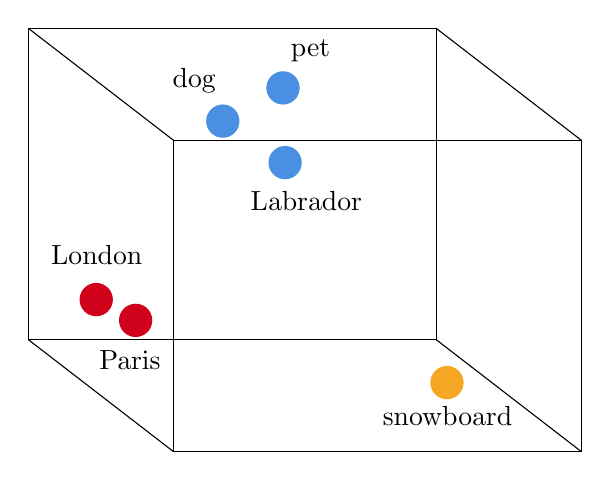
\begin{tikzpicture}[x=0.75pt,y=0.75pt,yscale=-1,xscale=1]
%uncomment if require: \path (0,300); %set diagram left start at 0, and has height of 300

%Shape: Rectangle [id:dp09766223150045761] 
\draw   (53,38) -- (249.5,38) -- (249.5,188) -- (53,188) -- cycle ;
%Shape: Rectangle [id:dp15444454726665247] 
\draw   (123,92) -- (319.5,92) -- (319.5,242) -- (123,242) -- cycle ;
%Straight Lines [id:da41180023590596115] 
\draw    (53,38) -- (123,92) ;


%Straight Lines [id:da8327746912035379] 
\draw    (53,188) -- (123,242) ;


%Straight Lines [id:da7076376732109662] 
\draw    (249.5,38) -- (319.5,92) ;


%Straight Lines [id:da531943191161679] 
\draw    (249.5,188) -- (319.5,242) ;


%Shape: Circle [id:dp5653236923369969] 
\draw  [color={rgb, 255:red, 74; green, 144; blue, 226 }  ,draw opacity=1 ][fill={rgb, 255:red, 74; green, 144; blue, 226 }  ,fill opacity=1 ] (168,66.75) .. controls (168,62.47) and (171.47,59) .. (175.75,59) .. controls (180.03,59) and (183.5,62.47) .. (183.5,66.75) .. controls (183.5,71.03) and (180.03,74.5) .. (175.75,74.5) .. controls (171.47,74.5) and (168,71.03) .. (168,66.75) -- cycle ;
%Shape: Circle [id:dp7862090364041379] 
\draw  [color={rgb, 255:red, 74; green, 144; blue, 226 }  ,draw opacity=1 ][fill={rgb, 255:red, 74; green, 144; blue, 226 }  ,fill opacity=1 ] (169,102.75) .. controls (169,98.47) and (172.47,95) .. (176.75,95) .. controls (181.03,95) and (184.5,98.47) .. (184.5,102.75) .. controls (184.5,107.03) and (181.03,110.5) .. (176.75,110.5) .. controls (172.47,110.5) and (169,107.03) .. (169,102.75) -- cycle ;
%Shape: Circle [id:dp04017773076556641] 
\draw  [color={rgb, 255:red, 74; green, 144; blue, 226 }  ,draw opacity=1 ][fill={rgb, 255:red, 74; green, 144; blue, 226 }  ,fill opacity=1 ] (139,82.75) .. controls (139,78.47) and (142.47,75) .. (146.75,75) .. controls (151.03,75) and (154.5,78.47) .. (154.5,82.75) .. controls (154.5,87.03) and (151.03,90.5) .. (146.75,90.5) .. controls (142.47,90.5) and (139,87.03) .. (139,82.75) -- cycle ;
%Shape: Circle [id:dp3593472220907403] 
\draw  [color={rgb, 255:red, 245; green, 166; blue, 35 }  ,draw opacity=1 ][fill={rgb, 255:red, 245; green, 166; blue, 35 }  ,fill opacity=1 ] (247,208.75) .. controls (247,204.47) and (250.47,201) .. (254.75,201) .. controls (259.03,201) and (262.5,204.47) .. (262.5,208.75) .. controls (262.5,213.03) and (259.03,216.5) .. (254.75,216.5) .. controls (250.47,216.5) and (247,213.03) .. (247,208.75) -- cycle ;
%Shape: Circle [id:dp42932079750070606] 
\draw  [color={rgb, 255:red, 208; green, 2; blue, 27 }  ,draw opacity=1 ][fill={rgb, 255:red, 208; green, 2; blue, 27 }  ,fill opacity=1 ] (78,168.75) .. controls (78,164.47) and (81.47,161) .. (85.75,161) .. controls (90.03,161) and (93.5,164.47) .. (93.5,168.75) .. controls (93.5,173.03) and (90.03,176.5) .. (85.75,176.5) .. controls (81.47,176.5) and (78,173.03) .. (78,168.75) -- cycle ;
%Shape: Circle [id:dp1106554795442356] 
\draw  [color={rgb, 255:red, 208; green, 2; blue, 27 }  ,draw opacity=1 ][fill={rgb, 255:red, 208; green, 2; blue, 27 }  ,fill opacity=1 ] (97,178.75) .. controls (97,174.47) and (100.47,171) .. (104.75,171) .. controls (109.03,171) and (112.5,174.47) .. (112.5,178.75) .. controls (112.5,183.03) and (109.03,186.5) .. (104.75,186.5) .. controls (100.47,186.5) and (97,183.03) .. (97,178.75) -- cycle ;

% Text Node
\draw (133,63) node   {dog};
% Text Node
\draw (189,49) node   {pet};
% Text Node
\draw (187,121) node   {Labrador};
% Text Node
\draw (255,225) node   {snowboard};
% Text Node
\draw (86,147) node   {London};
% Text Node
\draw (102,198) node   {Paris};


\end{tikzpicture}



}
\caption{An example of dense vector presentation of words in a 2-dimensional space, that maps words with similar meaning to nearby points.}
\label{fig:vsmodels}
\end{figure}
Traditional \emph{Natural Language Processing} (NLP) systems treat words as atomic units. Represented as vectors, each word would be treated as a one-hot vector (with $1$ in a single position and zero for the rest) with the size of the vocabulary. These vectors are sparse and orthogonal, and therefore contain no notion of similarity among themselves. For example, if a user is searching for \emph{``Heidelberg Hotel''}, documents containing \emph{``Heidelberg Motel''} are to be disregarded since the dot product of the one-hot vectors of \emph{``Hotel''} and \emph{``Motel''} is zero. On the other hand, distributed vector space models represent words in a continuous vector space, where a word is represented by its relation to the surrounding words. These models are based on the idea that similar words tend to occur in a similar context or as the British linguist J.R. Firth said:\\ \\
\noindent
\say{You shall know a word by the company it keeps.} (J.R. Firth 1957)\\
\\
These distributed representations try to map words to a dense vector, such that words with closer meanings are mapped to the nearby points and the similarity between them can be computed based on their distance in space. An example of the embedding space for such models is illustrated in Figure~\ref{fig:vsmodels}, where the vectors of \emph{``dog''},  \emph{``pet''} and, \emph{``labrador''} are mapped to nearby points and are farther away from unrelated words like \emph{``snowboard''}.
Learning dense vector representations of words dates back to $2000$ in the paper by Bengio et al., where they presented a neural probabilistic language model~\brackettext{\cite{DBLP:conf/nips/BengioDV00}}. The first simple and scalable algorithm, however, is \emph{word2vec} presented by \brackettext{\cite{DBLP:journals/corr/abs-1301-3781}}, where the aim is to capture the meaning of a word based on the surrounding context. There exist numerous variations of this model, from taking the character level information into account ~\brackettext{\cite{DBLP:journals/tacl/BojanowskiGJM17}} to incorporating the statistics of the whole corpus, namely the \emph{GloVe} model~\brackettext{\cite{DBLP:conf/emnlp/PenningtonSM14}}. The GloVe model in particular speeds up the learning and when trained on a large corpus tends to generate more promising results on downstream tasks such as named entity recognition.\\
Methods based on word2vec, despite being good at capturing semantics, have some drawbacks. They treat all words equally as terms and cannot be directly used to represent named entities. \emph{Named Entities} (NEs) refer to proper names or nouns and numerical expressions, such as dates and quantities~\brackettext{\cite{DBLP:conf/lrec/ToralMM08}}.
Many NLP tasks either depend on or use named entities as input. Identifying these references and classifying them has given rise to named entity recognition and disambiguation tasks. They are also extensively used in \emph{Information Retrial} (IR) and search engines. Disregarding the named entities while generating an embedding creates several challenges for downstream tasks that use them as input. Named entities often contain compound words and phrases, which, if not grouped together from the start, result in ambiguous and unclear embeddings. Although some work has been done on embedding phrases~\brackettext{\cite{DBLP:journals/tacl/HillCKB16,DBLP:conf/acl/YinS14}} or combining compound words after training with averaging, adding, or multiplying~\brackettext{\cite{DBLP:conf/eacl/DurmeRPM17,DBLP:journals/cogsci/MitchellL10}}, none of these focus on entities. The models that do focus on embedding entities, however, are designed for task specific applications, such as document ranking or named entity disambiguation~\brackettext{\cite{DBLP:conf/conll/YamadaS0T16,DBLP:conf/sigir/XiongCL17}}. These models are not only task-specific but also are focused on learning representations of \emph{knowledge base} (databases containing knowledge about named entities and their relation in a collection of documents) and do not focus on learning the entity embedding form a textual corpus.\\
A term-based model fails to distinguish between entity homographs such as  \emph{``Paris''},  which can refer to the French capital, the American heiress, or even the Trojan prince. Moreover, it cannot recognize any compound word. Any word separated by space is considered its own token, whereas many companies and actors names have two parts that not necessarily separate.  In a team-based model, if an entity is repeated several times with different names, a term-based model treats each name independently. In doing so, we lose valuable context information for the entity. Another drawback of term-based models is their inability to deal with date information. There exist multiple representations of date and time in text, e.g, $1$ January 1998 or $1998$-$01$-$01$T$15$:$53$:$00$, most models disregard any numeric information in text and limit themselves to a certain alphabet. With the exception of a few studies that try to add a temporal dimension to a paragraph or word embeddings, they mostly focus on how the embeddings evolve or change with time and do not achieve a vector presentation of dates~\brackettext{\cite{DBLP:conf/coling/MirzaT16a,DBLP:conf/ecir/YoonMWLK18}}.  \\
Another drawback of word embeddings in general is the lack of interpretability. In many cases, the semantic structure is heterogeneously distributed across the embedding dimensions, which makes interpretation challenging. Recently, some research has been done to make the embedding less ambiguous~\brackettext{\cite{DBLP:journals/corr/FaruquiTYDS15,DBLP:conf/emnlp/ParkBO17,DBLP:conf/aaai/SubramanianPJBH18}}. However, none of them show any insight about possible entity relations and most are applied as a post-processing step to the trained embedding. They offer no solution to learn the embeddings as an interpretable component during training time. There is no efficient method that can produce interpretable embeddings based on the entities surrounding a word. It is still unknown, what the implications are if a model predicts, for example  \emph{``London''} and \emph{``Berlin''} as similar. The dense vector representing the words does not show the reason behind their similarity. It is not obvious, whether they both appeared in the same context location-wise, e.g., whether both are capitals and are situated in Europe or because they share the same organizations, e.g., many companies planned to move their offices from London to Berlin after the Brexit and are mentioned in the same context. \\
Since named entities play an important rule in many NLP and IR tasks, a more intelligent representation of them enhances the performance of systems that utilize them as input features. Word embeddings are used for named entity recognition,linkage, and entity ranking~\brackettext{\cite{DBLP:conf/conll/EshelCRMYL17,DBLP:conf/nodalida/Siencnik15,DBLP:conf/icassp/MaKBK16}}, where a unique and unambiguous representation of entities can boost their performance.
Search engines, query expansion~\brackettext{\cite{DBLP:conf/acl/0001MC16,DBLP:conf/cikm/KuziSK16}}, and document ranking~\brackettext{\cite{DBLP:conf/sigir/ZamaniC17}} that utilize named entities can also benefit from a joint representation of words and entities.\\
On the other hand, annotating the text with named entities, requires extensive pre-processing, from sentence splitting and tokenization to part-of-speech tagging. Not only are these steps prone to errors, but also the task of recognizing and classifying the entities, even with the state-of-the-art tools, are far from perfect. Therefore, naively applying the word embedding methods to entity annotated text might have more problems than benefits. It is important that the drawbacks of such an approach alongside their advantages are analysed. 

% BR
%
% Good introduction, but it gets quickly bogged down in details.
% Everything important is there but you should rather present a single
% use case and expand from there. The idea of interspersing related work
% within the introduction is nice, but this could also become a separate
% section.

%%%%%%%%%%%%%%%%%%%%%%%%%%%%%%%%%%%%%%%%%%%%%%%%%%%%%%%%%%%%%%%%%%%%%%%%
\section{Objective and Contributions}
In this thesis, we address the problems of team-based models for generating embeddings for named entities as well as terms using an annotated corpus. In addition, to further analyze the importance of each entity type we experiment with faceted embeddings as a method to better understand the semantic structures and increase the interpretability of vector space models. Therefore, this thesis discusses two main models, one for the entity and term embeddings and one for the faceted model. Below, we will discuss the contribution of each separately.\\
By analysing the entity-based models we make the following contributions:
\begin{itemize}
\item We apply the state-of-the-art word embedding methods on an annotated corpus to jointly train terms and embeddings. 
\item We use graph embedding techniques to embed the nodes of a co-occurrence graph, extracted from the annotated text as an alternative means of obtaining entity embeddings. 
\item We evaluate both of our models against well-established word embedding methods on a set of intrinsic evaluation tasks. 
\item Since few test datasets contain any entities, we create some of our own, to better analyse the effect of entity annotation. 
\item Through visualization and experimental analysis, we investigate the underlying semantics that entity embeddings capture,  and discuss the implications for entity-centric downstream tasks.
\item By comparing the entity-based and word-based methods, we identify their strengths, weaknesses and application scenarios for both models.
\end{itemize}
To further analyse the impact of different types of entities on a certain entity embedding and to make the embeddings more interpretable we introduce faceted embedding. With the faceted model, we make following contributions: 
\begin{itemize}
\item We modify well-established word embedding techniques to include separable parts, where each part of the embedding corresponds to a specific type of entities. 
\item We use graph embedding techniques on a co-occurrence graph extracted from an annotated corpus to examine the relation of each word to the neighbours of a specific type. By embedding the nodes of such a graph we introduce an alternative way to achieve the faceted model.
\item We evaluate the faceted models against our entity-based models as well as word-based methods on raw text, based on word-centric intrinsic tasks. 
\item Since separate parts of faceted embeddings divide the embedding space into the different type of entities available in text, we investigate the effect of each type on intrinsic tasks. 
\item By visualizing the embedding parts separately, we explore potential use cases and the underlying semantics of such models.   
\end{itemize}

% BR: A good section, but the structure should be more succinct. When
% this is read (by the grader), I should immediately see what the
% objectives were and how they have been achieved. Maybe a different
% layout with 'at-a-glance' contributions would be helpful here. It is
% good that you use concrete examples, but there should be a brief
% summary about them.


%%%%%%%%%%%%%%%%%%%%%%%%%%%%%%%%%%%%%%%%%%%%%%%%%%%%%%%%%%%%%%%%%%%%%%%%
\section{Overview of the Thesis Structure}
The remainder of this thesis is structured as follows: 
In Chapter~\ref{chap:background},  we discuss the background information required for the model and related work, with a brief introduction to the basics of NLP and neural networks. This discussion is followed by, an explanation of well-established word embedding and graph embedding methods, which are the base of the entity and faceted embeddings.\\
In Chapter~\ref{chap:entity}, two types of models for learning terms and entity embeddings jointly on an annotated corpus are presented. One method focuses on learning the vector representation from a textual corpus, while the other method requires a co-occurrence graph extracted from the annotated text.
Chapter~\ref{chap:faceted} contains an in-depth definition of the faceted embeddings,where different models are proposed based on the input data (textual or graph-based). 
In Chapter~\ref{chap:eval}, the test cases and evaluation results are presented. The entity embeddings and faceted models are analysed using visualizations and also tested against well-known analogy, word similarity and categorization datasets.
The work is closed with a conclusion and outlook on possible future work in Chapter~\ref{chap:concl}. 


% BR: Very nice in total. I would recommend the following, though:
%  - make the claims more concise and precise
%  - formulate the objectives and how this was achieved.
%  - ideally, you can formulate both at the same time and place
%  - for example, I had 'Contributions' in my dissertation as well, you
%    may want to look at these (text me if you have troubles finding
%    that)

  %%%%%%%%%%%%%%%%%%%%%%%%%%%%%%%%%%%%%%%%%%%%%%%%%%%%%%%%%%%%

\chapter{Background and Related Work}\label{chap:background}
To generate a vector representation of named entities and terms in an annotated document, we use either a corpus of text with entity annotations or the co-occurrence graph extracted from it. Unlike traditional methods, where all tokens are treated as terms, entity embeddings take the type information into account. To provide a general background for all the methods used in this thesis, the related work and background is organized as follows:\\
In Section~\ref{sec:NLP} a brief overview of the text preprocessing steps for NLP tasks is given, in which methods used to extract information from text or common preprocessing steps are explained, containing text cleaning, stemming, lemmatization, part-of-speech tagging, named entity recognition and linkage. In Section~\ref{sec:nn} neural network based approaches for learning embeddings are explained. The co-occurrence graphs are explained in Section~\ref{sec:graph} along with the LOAD model~\brackettext{\cite{DBLP:conf/sigir/SpitzG16}}, which is a specific co-occurrence graph used in this thesis. Since word2vec and GloVe are the building blocks of other models, they are described in Section~\ref{sec:wordembeddig}. In the same section, we also explain the generation of  weighted adjacency matrix from a weighted co-occurrence graph, which is comparable to a co-occurrence matrix in the GloVe model. In Section~\ref{sec:enity_embed}, we discuss the related work on generating entity embedding.  Finally, an overview of the important graph embedding methods is given in Section~\ref{sec:graph}, containing DeepWalk, node2vec, LINE, and VERSE. These models are used  in Chapter~\ref{chap:entity} and~\ref{chap:faceted} to create the entity and faceted embeddings, respectively. 

% BR: I would prefer this section to be more active: Section X provides
% Y. Other than that, no complaints. It is very nice that you are able
% to 'mix' background and related work. I like this.
%%%%%%%%%%%%%%%%%%%%%%%%%%%%%%%%%%%%%%%%%%%%%%%%%%%%%%%%%%%%
\section{Basics of Natural Language Processing}\label{sec:NLP}
The goal of NLP systems is to understand and derive meaning from human language, with textual data as their main source of information.
Most of the World Wide Web is made of text, with websites, such as Twitter generating vast amounts every day. Analysing this content is, however, not a simple task. For example, human generated text often contains ambiguity, as in the sentence \emph{``I put my \textbf{wallet} in the  \textbf{car}.  \textbf{It} is green.''} In this sentence, it is not obvious if \emph{``it''} refers to the \emph{``car''} or the  \emph{``wallet''}. Moreover, humans often use homographs (words that have the same spelling but different meanings), metaphors and sarcasm, which further increases the complexity of text analysis.\\
As machine learning systems typically rely on features, the most important step is to derive features from the text. Multiple models have been proposed for feature extraction, and while none of them achieve the goal of fully characterizing a text, their utility differs.
% BR: 'more useful' is colloquial (which is not necessarily bad)
% BR: alt.: 'their utility differs'?
%
However, all features require cleaning and preprocessing of the text. 

% BR: general comment on this section: I am not sure I want to agree
% with the sentence on 'features', though. Some representations in ML
% are able to 'learn' the proper features on their own, right? Maybe
% you could add 'typically' here?
%%%%%%%%%%%%%%%%%%%%%%%%%%%%%%%%%%%%%%%%%%%%%%%%%%%%%%%%%%%%
\subsection{Text cleaning}\label{subsec:cleaning}
Before any operation can be performed on text, each sentence has to be broken down to its atomic pieces. \emph{Tokenization} is the act of chopping sentences up into pieces, called \emph{tokens}. For example, the sentence: \emph{``Tokenization is widely used in natural language processing.''}, can be tokenized as follows:\\

\mybox{Tokenization} \mybox{is} \mybox{widely} \mybox{used} \mybox{in} \mybox{natural language processing.}\\
\\
% BR: I find the punctuation of the example sentence slightly confusing.
% Maybe you should add quotes?
Splitting only by white spaces can also separate what should be regarded as a single token. For example, separating by white space would result into three tokens for \emph{``natural language processing''}. In a later section, we discuss named entity recognition that tries to eliminate such problems. \\
Text data has also many inconsistencies that can cause troubles for algorithms. Some common initial preprocessing steps to decrease these inconsistencies are to convert all of the letters to lowercase and to remove punctuation.
This makes sure that \emph{``analytics''}, \emph{``AnALYticS''}, \emph{``Analytics!''}, and \emph{``\#analytics''} are all considered the same word. Removing punctuation should be applied with care, because in some cases, such as in the case of Twitter \emph{``\#analytics''} is a message about analytics and should not be confused with \emph{``@analytics''}, which is a message to the analytics account. For these reasons, the removal of punctuation should be tailored to the specific problem.\\
% BR: Very nice! For the last sentence: can you give resources that
% describe how to tailor this to specific problems?
%TODO find a citation ! 
Additionally, words such as, \emph{``are''} and \emph{``to''} are frequent in all documents but are only meaningful in a sentence. These are called \emph{stop-words}. Despite the high frequency, these words are unlikely to result in a meaningful feature for a machine learning system and are often removed~\brackettext{\cite{ACM:Manning:1999:FSN:311445},\cite{ACM:Jurafsky:2000:SLP:555733}}. As with punctuation, removing stop words blindly may result in loss of valuable information. For example, \emph{``The Who''} is the name of a band, and naive stop word removal might delete those words even if they carry significant meaning. Hence, removing all stop-words is not always helpful, but it is generally considered to be a useful step. 
% BR: Can you give a citation for this? Maybe rewrite it so that it
% becomes a 'best practice'?
%%%%%%%%%%%%%%%%%%%%%%%%%%%%%%%%%%%%%%%%%%%%%%%%%%%%%%%%%%%%
\subsection{Stemming and  lemmatization}\label{subsec:steming}
Another important preprocessing step is \emph{stemming} or \emph{lemmatization}. This step is motivated by the desire to represent verbs with different grammatical conjugations as the same word.
% BR: I would be more precise about the different endings here. Can you
% specify that this pertains to 'grammatical endings' here?
In many cases, there is no need for a distinction between \emph{argue}, \emph{argued}, \emph{argues}, and \emph{arguing}. They could all be represented by a common stem: \emph{argu}. This is called stemming as it chops off the ends of words and often includes the removal of derivational affixes. Another approach is lemmatization, that uses the vocabulary and morphological analysis of words, normally aiming to remove inflectional endings only and to return the base or dictionary form of a word, which is known as the \emph{lemma}. Lemmatization is a more complex procedure as it requires detailed dictionaries, which the algorithm has to look through, to link a specific form back to its lemma. This is particularly problematic for irregular verbs, where the past and present tense of a verb do not share the same stem. For instance,
the lemmatization of \emph{``drank''} is \emph{``drink''}~\brackettext{\cite{SCHOL:book/larson2010,ACM:Jurafsky:2000:SLP:555733}}.
% BR: The last sentence should be rewritten: 
% > This is particularly problematic for irregular verbs. For instance,
% > the lemmatization of ``drank'' is ``drink''.
%%%%%%%%%%%%%%%%%%%%%%%%%%%%%%%%%%%%%%%%%%%%%%%%%%%%%%%%%%%%
\subsection{Part-of-speech tagging (POS tagging)}\label{subsec:pos}
\emph{POS tagging} is the process of assiging a\emph{ part of speech} to each word in text. Parts of speech are also known as \emph{word classes} or \emph{lexical categories} are categories to which a word is assigned in accordance with its syntactic functions (e.g., noun, verb, adjective,~\dots). POS tags are useful because they yield a large amount of information about a word and the syntactic context around a word~\brackettext{\cite{ACM:Manning:1999:FSN:311445, ACM:Jurafsky:2000:SLP:555733}}. Parts of speech are useful features for finding named entities, such as people or organizations in text~\brackettext{\cite{SCHOL:book/jurafsky2016}}. Applications that provide POS tagging are also referred to as \emph{POS taggers}, which are used to assign tags to tokens using a finite predefined tagset. For English, the most commonly used tagset is the \textbf{Penn Treebank POS tagset} \footcite{https://www.ling.upenn.edu/courses/Fall_2003/ling001/penn_treebank_pos.html}. 
% BR: I would change the sentence about the software. Maybe refer to it
% in an active fashion, e.g. 'Applications that provide POS tagging are
% also referred to as POS taggers'.
%%%%%%%%%%%%%%%%%%%%%%%%%%%%%%%%%%%%%%%%%%%%%%%%%%%%%%%%%%%%
\subsection{Named entity recognition and  entity linking}\label{subsec:entity_recog}
\emph{Named Entity Recognition} (NER)  or \emph{entity extraction} is an information extraction method that locates and classifies the named entities in text. Named entities are words that can be classified into a set of pre-defined classes, such as the names of persons, organizations, locations, quantities and monetary values. In some cases, temporal expressions are classified separately as well. Generally, anything that is not an entity per se is considered to be a term~\brackettext{\cite{SCHOL:journal/LI/nadeau}}. More formally, if we define $V$ as the set of all words in the vocabulary, $N\subseteq V$ is the set of all entities that fall into a pre-defined category.
% BR: this seems mathematically inconsistent: if the entities are
% a subset of the terms, you cannot say that anything else is a term,
% because that would make it _not_ a subset again.
Recognition of entities is difficult, partly because of ambiguities and mostly because of multiple surface forms (different names for the same entity).
% BR: what kind of ambiguities are we talking about?
% BR: what is a surface form?
It is not always clear what is or is not an entity or what type it has. For example, the entity \emph{``Washington''} can be a name of a city, a person or even an organization. NER identifies the occurrence or mention of a named entity in the text, but it does not identify which specific entity it is. \emph{Named entity linking} (NEL) or \emph{named entity disambiguation} (NED) is the task of mapping the found entities to a repository of entities. For this purpose, \emph{knowledge bases} or \emph{knowledge graphs} are used, which contain rich information about the entities and their mutual relationships~\brackettext{\cite{ACM:Manning:1999:FSN:311445,ACM:Jurafsky:2000:SLP:555733}}. Knowledge graph is a repository of structured information consisting of unique entities, facts about entities ,and relations between entities. NEL maps the found entities to their corresponding entry in the knowledge base~\brackettext{\cite{DBLP:journals/tkde/ShenWH15}}. 
% BR: can you give a link to a section with more information about this?
% BR: very nice; maybe you could add a brief description of 'entity' in
% parenthesis after first mentioning it.
%%%%%%%%%%%%%%%%%%%%%%%%%%%%%%%%%%%%%%%%%%%%%%%%%%%%%%%%%%%%
\section{Neural Networks in Natural Language Processing}\label{sec:nn}
Before the advancements in deep learning and neural networks, most NLP techniques were based on machine learning approaches with linear models such as support vector machines or logistic regression, trained on very high-dimensional and sparse feature vectors. Recently, the field has changed to use non-linear neural-network models over dense inputs. The most important advantage of such methods is that they can often be trained with a single end-to-end model and do not require traditional task-specific feature engineering~\brackettext{\cite{DBLP:journals/jair/Goldberg16}}. Methods for different NLP tasks differ in architectures of neural networks and feature representations. Since the focus of this thesis is on word and entity embeddings, we focus on simple neural networks and the basic idea needed to generate word embeddings.
%%%%%%%%%%%%%%%%%%%%%%%%%%%%%%%%%%%%%%%%%%%%%%%%%%%%%%%%%%%%
\subsection{Neural networks}

\begin{figure}
\centering 
\resizebox{0.65\textwidth}{0.35\textwidth}{      
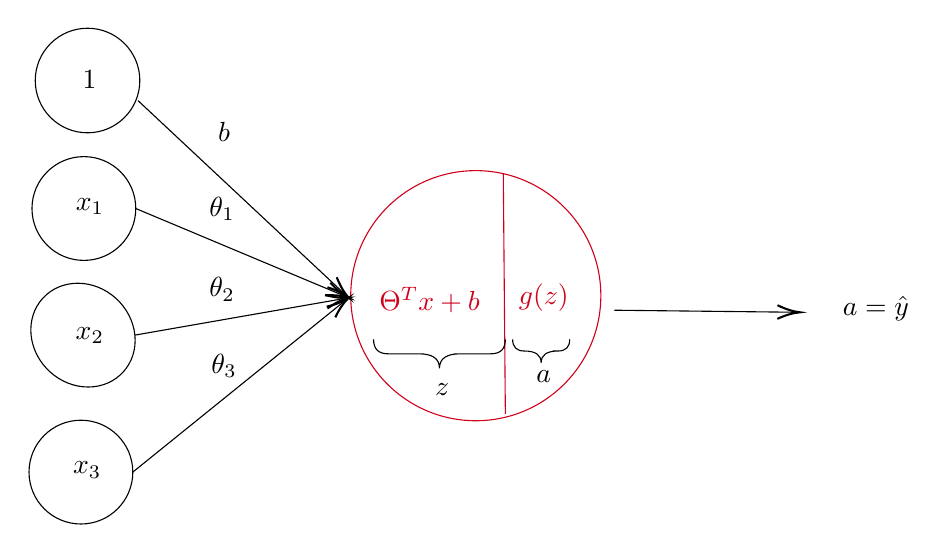
\begin{tikzpicture}[x=0.75pt,y=0.75pt,yscale=-1,xscale=1]
%uncomment if require: \path (0,300); %set diagram left start at 0, and has height of 300

%Shape: Circle [id:dp4894456216466021] 
\draw   (73.43,102) .. controls (73.43,88.19) and (84.63,77) .. (98.43,77) .. controls (112.24,77) and (123.43,88.19) .. (123.43,102) .. controls (123.43,115.81) and (112.24,127) .. (98.43,127) .. controls (84.63,127) and (73.43,115.81) .. (73.43,102) -- cycle ;
%Shape: Circle [id:dp5135503842228779] 
\draw   (73,163) .. controls (71.62,149.19) and (81.69,138) .. (95.5,138) .. controls (109.31,138) and (121.62,149.19) .. (123,163) .. controls (124.38,176.81) and (114.31,188) .. (100.5,188) .. controls (86.69,188) and (74.38,176.81) .. (73,163) -- cycle ;
%Shape: Circle [id:dp5054751399658592] 
\draw   (72,229) .. controls (72,215.19) and (83.19,204) .. (97,204) .. controls (110.81,204) and (122,215.19) .. (122,229) .. controls (122,242.81) and (110.81,254) .. (97,254) .. controls (83.19,254) and (72,242.81) .. (72,229) -- cycle ;
%Shape: Circle [id:dp7068247835752886] 
\draw  [color={rgb, 255:red, 208; green, 2; blue, 27 }  ,draw opacity=1 ] (227,144) .. controls (227,110.72) and (253.97,83.75) .. (287.25,83.75) .. controls (320.53,83.75) and (347.5,110.72) .. (347.5,144) .. controls (347.5,177.28) and (320.53,204.25) .. (287.25,204.25) .. controls (253.97,204.25) and (227,177.28) .. (227,144) -- cycle ;
%Straight Lines [id:da3951259360286594] 
\draw    (123.43,102) -- (224.16,144.23) ;
\draw [shift={(226,145)}, rotate = 202.75] [color={rgb, 255:red, 0; green, 0; blue, 0 }  ][line width=0.75]    (10.93,-3.29) .. controls (6.95,-1.4) and (3.31,-0.3) .. (0,0) .. controls (3.31,0.3) and (6.95,1.4) .. (10.93,3.29)   ;

%Straight Lines [id:da17712089576257095] 
\draw    (123,163) -- (224.03,145.34) ;
\draw [shift={(226,145)}, rotate = 530.0899999999999] [color={rgb, 255:red, 0; green, 0; blue, 0 }  ][line width=0.75]    (10.93,-3.29) .. controls (6.95,-1.4) and (3.31,-0.3) .. (0,0) .. controls (3.31,0.3) and (6.95,1.4) .. (10.93,3.29)   ;

%Straight Lines [id:da10379609280096158] 
\draw    (122,229) -- (224.44,146.26) ;
\draw [shift={(226,145)}, rotate = 501.07] [color={rgb, 255:red, 0; green, 0; blue, 0 }  ][line width=0.75]    (10.93,-3.29) .. controls (6.95,-1.4) and (3.31,-0.3) .. (0,0) .. controls (3.31,0.3) and (6.95,1.4) .. (10.93,3.29)   ;

%Straight Lines [id:da1555895906794451] 
\draw    (354,151) -- (441.5,151.98) ;
\draw [shift={(443.5,152)}, rotate = 180.64] [color={rgb, 255:red, 0; green, 0; blue, 0 }  ][line width=0.75]    (10.93,-3.29) .. controls (6.95,-1.4) and (3.31,-0.3) .. (0,0) .. controls (3.31,0.3) and (6.95,1.4) .. (10.93,3.29)   ;

%Shape: Circle [id:dp07492513539205437] 
\draw   (75,40.33) .. controls (75,26.42) and (86.28,15.14) .. (100.19,15.14) .. controls (114.1,15.14) and (125.38,26.42) .. (125.38,40.33) .. controls (125.38,54.24) and (114.1,65.52) .. (100.19,65.52) .. controls (86.28,65.52) and (75,54.24) .. (75,40.33) -- cycle ;
%Straight Lines [id:da37710728737628485] 
\draw    (124.5,50) -- (224.54,143.63) ;
\draw [shift={(226,145)}, rotate = 223.11] [color={rgb, 255:red, 0; green, 0; blue, 0 }  ][line width=0.75]    (10.93,-3.29) .. controls (6.95,-1.4) and (3.31,-0.3) .. (0,0) .. controls (3.31,0.3) and (6.95,1.4) .. (10.93,3.29)   ;

%Straight Lines [id:da9942335357246543] 
\draw [color={rgb, 255:red, 208; green, 2; blue, 27 }  ,draw opacity=1 ]   (300.5,85) -- (301.5,201) ;


%Shape: Brace [id:dp48208896309529936] 
\draw   (238,165) .. controls (238,169.67) and (240.33,172) .. (245,172) -- (259.75,172) .. controls (266.42,172) and (269.75,174.33) .. (269.75,179) .. controls (269.75,174.33) and (273.08,172) .. (279.75,172)(276.75,172) -- (294.5,172) .. controls (299.17,172) and (301.5,169.67) .. (301.5,165) ;
%Shape: Brace [id:dp308784031815875] 
\draw   (305,165) .. controls (305,168.77) and (306.89,170.66) .. (310.66,170.66) -- (310.66,170.66) .. controls (316.05,170.66) and (318.75,172.55) .. (318.75,176.32) .. controls (318.75,172.55) and (321.45,170.66) .. (326.84,170.66)(324.41,170.66) -- (326.84,170.66) .. controls (330.61,170.66) and (332.5,168.77) .. (332.5,165) ;

% Text Node
\draw (101.3,163) node   {$x_{2}$};
% Text Node
\draw (101.37,100.96) node   {$x_{1}$};
% Text Node
\draw (100,228) node   {$x_{3}$};
% Text Node
\draw (101.21,39.84) node   {$1$};
% Text Node
\draw (166,65) node   {$b$};
% Text Node
\draw (165,102) node   {$\theta _{1}$};
% Text Node
\draw (165,141) node   {$\theta _{2}$};
% Text Node
\draw (166,178) node   {$\theta _{3}$};
% Text Node
\draw (480,150) node   {$a=\hat{y}$};
% Text Node
\draw (320,145) node [color={rgb, 255:red, 208; green, 2; blue, 27 }  ,opacity=1 ]  {$g( z)$};
% Text Node
\draw (265,146) node [color={rgb, 255:red, 208; green, 2; blue, 27 }  ,opacity=1 ]  {$\Theta ^{T} x+b$};
% Text Node
\draw (271,189) node   {$z$};
% Text Node
\draw (320,183) node   {$a$};


\end{tikzpicture}


}
\caption{Single layer neural network. The input $x$ is multiplied by the matrix of weights $\Theta$ to be passed to the activation function (a typically non-linear function to transform the input) to generate the output $\hat { y }$. \protect \footnotemark}
% BR: you should also mention the activation function here and give an
% example.
\label{fig:preceptron}
\end{figure}
\footnotetext{The figure is adapted from https://www.coursera.org/learn/machine-learning.}
\noindent
Despite neural networks being the new trend in machine learning, they are rather old algorithms, which are motivated by the goal of having a machine that mimics a brain. The sudden resurgence of neural networks is due to the fact that they are computationally expensive and require a huge amounts of data, which was neither available nor processable in the 80s and 90s. Also \emph{``backpropagation''} algorithm~\brackettext{\cite{SCHOL:journals/nature/rumelhart1986learning}} and the advent of GPUs, sped up the training process and made it feasible to train models with thousands of parameters.\\
A single artificial neuron, consisting of a single computational unit, is shown in Figure~\ref{fig:preceptron}. The computational unit illustrated in red takes in the different features of the input $x_i$ and multiplies each with a given weight $\theta_i$. The result of the multiplication is added to the \emph{bias unit} $b$ that always has an input value of $1$.
The weights indicate the importance of each feature for the computation and are learnable parameters of the model. The neuron then performs a transformation to the input through the \emph{activation function} ($g(x)$) and generates the output ($\hat { y } $). The activation function is typically non-linear transformation that is applied on the input data.\\
% BR: the non-linearity arises from the activation function; you should
% mention this. Moreover, you can select a linear activation function if
% you want.  I would thus rather say that they are 'typically selected
% to be non-linear' or something similar.
Essentially, each neuron consists of two steps of computation. First, intermediate output $z$ is computed by the multiplication of weights with input features, which is a linear operation that boils down to a matrix--vector product.
Second, an activation function of choice is applied to $z$ to produce the final output or activation ($a$) of the last unit. \\
\begin{figure}
\centering 
\resizebox{0.75\textwidth}{0.45\textwidth}{      
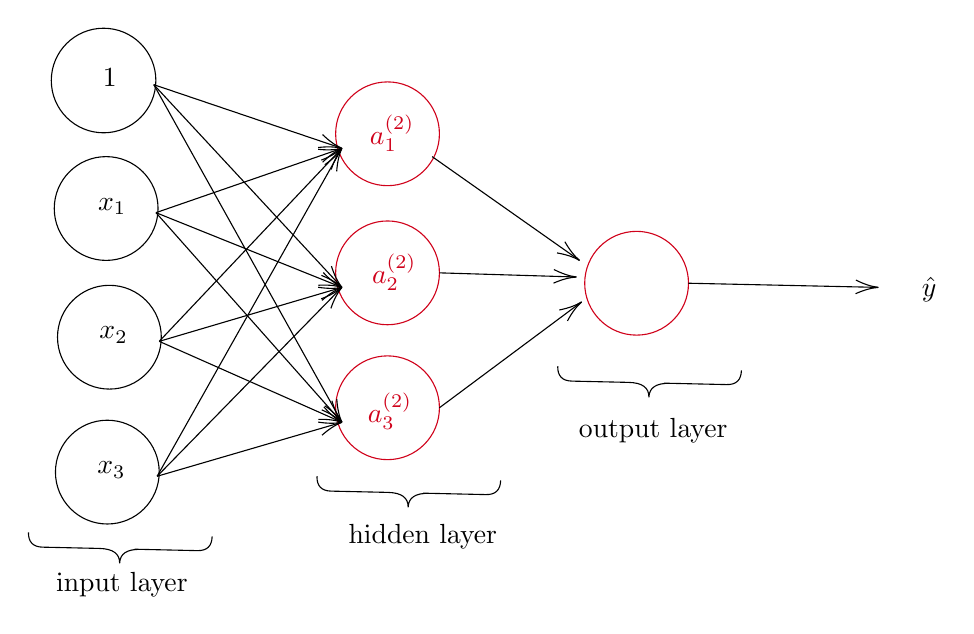
\begin{tikzpicture}[x=0.75pt,y=0.75pt,yscale=-1,xscale=1]
%uncomment if require: \path (0,300); %set diagram left start at 0, and has height of 300

\draw  [color={rgb, 255:red, 208; green, 2; blue, 27 }  ,draw opacity=1 ]  (241, 71) circle [x radius= 25, y radius= 25]  ;
\draw  [color={rgb, 255:red, 208; green, 2; blue, 27 }  ,draw opacity=1 ]  (241, 138) circle [x radius= 25, y radius= 25]  ;
\draw  [color={rgb, 255:red, 208; green, 2; blue, 27 }  ,draw opacity=1 ]  (241, 203) circle [x radius= 25, y radius= 25]  ;
\draw    (262.5,82) -- (333.5,132) ;
\draw [shift={(333.5,132)}, rotate = 215.15] [color={rgb, 255:red, 0; green, 0; blue, 0 }  ]   (0,0) .. controls (3.31,-0.3) and (6.95,-1.4) .. (10.93,-3.29)(0,0) .. controls (3.31,0.3) and (6.95,1.4) .. (10.93,3.29)   ;

\draw    (266,138) -- (332,140) ;
\draw [shift={(332,140)}, rotate = 181.74] [color={rgb, 255:red, 0; green, 0; blue, 0 }  ]   (0,0) .. controls (3.31,-0.3) and (6.95,-1.4) .. (10.93,-3.29)(0,0) .. controls (3.31,0.3) and (6.95,1.4) .. (10.93,3.29)   ;

\draw    (266,203) -- (334.5,152) ;
\draw [shift={(334.5,152)}, rotate = 503.33] [color={rgb, 255:red, 0; green, 0; blue, 0 }  ]   (0,0) .. controls (3.31,-0.3) and (6.95,-1.4) .. (10.93,-3.29)(0,0) .. controls (3.31,0.3) and (6.95,1.4) .. (10.93,3.29)   ;

\draw  [color={rgb, 255:red, 208; green, 2; blue, 27 }  ,draw opacity=1 ]  (361, 143) circle [x radius= 25, y radius= 25]  ;
\draw    (386,143) -- (477.5,145) ;
\draw [shift={(477.5,145)}, rotate = 181.25] [color={rgb, 255:red, 0; green, 0; blue, 0 }  ]   (0,0) .. controls (3.31,-0.3) and (6.95,-1.4) .. (10.93,-3.29)(0,0) .. controls (3.31,0.3) and (6.95,1.4) .. (10.93,3.29)   ;

\draw    (105.43, 107) circle [x radius= 25, y radius= 25]  ;
\draw    (107, 169) circle [x radius= 25, y radius= 25]  ;
\draw    (106, 234) circle [x radius= 25, y radius= 25]  ;
\draw    (104.19, 45.33) circle [x radius= 25.19, y radius= 25.19]  ;
\draw    (128.38,47.33) -- (219,78) ;
\draw [shift={(219,78)}, rotate = 198.7] [color={rgb, 255:red, 0; green, 0; blue, 0 }  ]   (0,0) .. controls (3.31,-0.3) and (6.95,-1.4) .. (10.93,-3.29)(0,0) .. controls (3.31,0.3) and (6.95,1.4) .. (10.93,3.29)   ;

\draw    (128.38,47.33) -- (219,145) ;
\draw [shift={(219,145)}, rotate = 227.14] [color={rgb, 255:red, 0; green, 0; blue, 0 }  ]   (0,0) .. controls (3.31,-0.3) and (6.95,-1.4) .. (10.93,-3.29)(0,0) .. controls (3.31,0.3) and (6.95,1.4) .. (10.93,3.29)   ;

\draw    (128.38,47.33) -- (219,210) ;
\draw [shift={(219,210)}, rotate = 240.88] [color={rgb, 255:red, 0; green, 0; blue, 0 }  ]   (0,0) .. controls (3.31,-0.3) and (6.95,-1.4) .. (10.93,-3.29)(0,0) .. controls (3.31,0.3) and (6.95,1.4) .. (10.93,3.29)   ;

\draw    (129.43,109) -- (219,210) ;
\draw [shift={(219,210)}, rotate = 228.43] [color={rgb, 255:red, 0; green, 0; blue, 0 }  ]   (0,0) .. controls (3.31,-0.3) and (6.95,-1.4) .. (10.93,-3.29)(0,0) .. controls (3.31,0.3) and (6.95,1.4) .. (10.93,3.29)   ;

\draw    (129.43,109) -- (219,145) ;
\draw [shift={(219,145)}, rotate = 201.9] [color={rgb, 255:red, 0; green, 0; blue, 0 }  ]   (0,0) .. controls (3.31,-0.3) and (6.95,-1.4) .. (10.93,-3.29)(0,0) .. controls (3.31,0.3) and (6.95,1.4) .. (10.93,3.29)   ;

\draw    (129.43,109) -- (219,78) ;
\draw [shift={(219,78)}, rotate = 520.9100000000001] [color={rgb, 255:red, 0; green, 0; blue, 0 }  ]   (0,0) .. controls (3.31,-0.3) and (6.95,-1.4) .. (10.93,-3.29)(0,0) .. controls (3.31,0.3) and (6.95,1.4) .. (10.93,3.29)   ;

\draw    (131,171) -- (219,78) ;
\draw [shift={(219,78)}, rotate = 493.42] [color={rgb, 255:red, 0; green, 0; blue, 0 }  ]   (0,0) .. controls (3.31,-0.3) and (6.95,-1.4) .. (10.93,-3.29)(0,0) .. controls (3.31,0.3) and (6.95,1.4) .. (10.93,3.29)   ;

\draw    (131,171) -- (219,145) ;
\draw [shift={(219,145)}, rotate = 523.54] [color={rgb, 255:red, 0; green, 0; blue, 0 }  ]   (0,0) .. controls (3.31,-0.3) and (6.95,-1.4) .. (10.93,-3.29)(0,0) .. controls (3.31,0.3) and (6.95,1.4) .. (10.93,3.29)   ;

\draw    (131,171) -- (219,210) ;
\draw [shift={(219,210)}, rotate = 203.9] [color={rgb, 255:red, 0; green, 0; blue, 0 }  ]   (0,0) .. controls (3.31,-0.3) and (6.95,-1.4) .. (10.93,-3.29)(0,0) .. controls (3.31,0.3) and (6.95,1.4) .. (10.93,3.29)   ;

\draw    (130,236) -- (219,78) ;
\draw [shift={(219,78)}, rotate = 479.39] [color={rgb, 255:red, 0; green, 0; blue, 0 }  ]   (0,0) .. controls (3.31,-0.3) and (6.95,-1.4) .. (10.93,-3.29)(0,0) .. controls (3.31,0.3) and (6.95,1.4) .. (10.93,3.29)   ;

\draw    (130,236) -- (219,145) ;
\draw [shift={(219,145)}, rotate = 494.36] [color={rgb, 255:red, 0; green, 0; blue, 0 }  ]   (0,0) .. controls (3.31,-0.3) and (6.95,-1.4) .. (10.93,-3.29)(0,0) .. controls (3.31,0.3) and (6.95,1.4) .. (10.93,3.29)   ;

\draw    (130,236) -- (219,210) ;
\draw [shift={(219,210)}, rotate = 523.72] [color={rgb, 255:red, 0; green, 0; blue, 0 }  ]   (0,0) .. controls (3.31,-0.3) and (6.95,-1.4) .. (10.93,-3.29)(0,0) .. controls (3.31,0.3) and (6.95,1.4) .. (10.93,3.29)   ;

\draw   (68,263) .. controls (67.89,267.67) and (70.17,270.05) .. (74.84,270.16) -- (102.1,270.77) .. controls (108.76,270.92) and (112.04,273.32) .. (111.93,277.99) .. controls (112.04,273.32) and (115.42,271.07) .. (122.09,271.22)(119.09,271.15) -- (149.34,271.83) .. controls (154.01,271.94) and (156.39,269.66) .. (156.5,264.99) ;
\draw   (207,236) .. controls (206.89,240.67) and (209.17,243.05) .. (213.84,243.16) -- (241.1,243.77) .. controls (247.76,243.92) and (251.04,246.32) .. (250.93,250.99) .. controls (251.04,246.32) and (254.42,244.07) .. (261.09,244.22)(258.09,244.15) -- (288.34,244.83) .. controls (293.01,244.94) and (295.39,242.66) .. (295.5,237.99) ;
\draw   (323,183) .. controls (322.89,187.67) and (325.17,190.05) .. (329.84,190.16) -- (357.1,190.77) .. controls (363.76,190.92) and (367.04,193.32) .. (366.93,197.99) .. controls (367.04,193.32) and (370.42,191.07) .. (377.09,191.22)(374.09,191.15) -- (404.34,191.83) .. controls (409.01,191.94) and (411.39,189.66) .. (411.5,184.99) ;

\draw (243.21,70.84) node [color={rgb, 255:red, 208; green, 2; blue, 27 }  ,opacity=1 ]  {$a^{( 2)}_{1}$};
\draw (244.21,137.84) node [color={rgb, 255:red, 208; green, 2; blue, 27 }  ,opacity=1 ]  {$a^{( 2)}_{2}$};
\draw (242.21,204.84) node [color={rgb, 255:red, 208; green, 2; blue, 27 }  ,opacity=1 ]  {$a^{( 2)}_{3}$};
\draw (109,168) node   {$x_{2}$};
\draw (108.37,105.96) node   {$x_{1}$};
\draw (108,233) node   {$x_{3}$};
\draw (107.21,43.84) node   {$1$};
\draw (502,146) node   {$\hat{y}$};
\draw (113,288) node   {input layer};
\draw (258,265) node   {hidden layer};
\draw (369,214) node   {output layer};


\end{tikzpicture}

}
\caption{Two layer neural network with one hidden layer. An input $x$ with three features is multiplied by the weight matrix $\Theta$ to generate an intermediate activation value $a$. The predicted output $\hat { y } $ is generated using the activations of the hidden layer.  \protect \footnotemark .}

\label{fig:nn}

\end{figure}
\noindent
A neural network is a group of multiple neurons connected together, as shown in Figure~\ref{fig:nn}. In a neural network, the first layer is called the \emph{input layer}, the last layer is called the \emph{output layer} and all other layers are referred to as \emph{hidden layers}.
Typically, the values of the input and the output layer (labels) are given in the training set. The output of each computational unit in the network is the activation of that unit. We denote activation of the unit (neuron) $i$ in layer $j$ by $a_{i}^{[j]}$. The weights of the network are the parameters of the model and learning them is goal of any neural network. We denote the weight controlling the function mapping from unit $n$ in layer $j$ to unit $l$ in layer $j+1$ by
$\theta^{(j)}_{nl}$. The weights indicate how different features of inputs should be combined and how much should each of them influence the final output. The values of intermediate activations can be interpreted as latent features discovered during training~\brackettext{\cite{SCHOL:book/haykin2009}}. As the network gets deeper, more complex combinations of input features can be learned. \\
An example of forward computation, which is called \emph{forward propagation}, for the network in Figure~\ref{fig:nn} is given in Equation~\ref{eq:nn_eq}. Although a single output is shown the figure, the output layer can have different sizes. It can vary from one output for a single class classification even $10,000$ pixels of a image. The number of hidden layers can also vary, where the next hidden layer would use the activation of the pervious layer as input. How different neurons connect, the choice of activation function, the shape of the output layer and the number of layers is what defines different architectures~\brackettext{\cite{SCHOL:Goodfellow-et-al-2016}}. Since most of literature on word embeddings focus on shallow neural networks, in this thesis, we focus only on networks with a few hidden layers. 
\begin{equation}
\begin{split}
a_{ 1 }^{ [2] }=g(\theta _{ 10 }^{ [1] }x_{ 0 }+\theta _{ 11 }^{ [1]}x_{ 1 }+\theta _{ 12 }^{ [1] }x_{ 2 }+\theta _{ 13 }^{ [1] }x_{ 3 })\\ 
a_{ 2 }^{ [2] }=g(\theta _{ 20 }^{ [1] }x_{ 0 }+\theta _{ 21 }^{ [1] }x_{ 1 }+\theta _{ 22 }^{ [1] }x_{ 2 }+\theta _{ 23 }^{ [1] }x_{ 3 })\\
 a_{ 3 }^{ [2] }=g(\theta _{ 30 }^{ [1] }x_{ 0 }+\theta _{ 31 }^{ [1] }x_{ 1 }+\theta _{ 32 }^{ [1] }x_{ 2 }+\theta _{ 33 }^{ [1] }x_{ 3 })\\
  \hat { y } =a_{ 1 }^{ [3] }=g(\theta _{ 10 }^{ [2] }x_{ 0 }+\theta _{ 11 }^{ [2] }x_{ 1 }+\theta _{ 12 }^{ [2] }x_{ 2 }+\theta _{ 13 }^{ [2] }x_{ 3 })
\end{split}
\label{eq:nn_eq}
\end{equation}
\footnotetext{The figure is adapted from https://www.coursera.org/learn/neural-networks-deep-learning.}
Activation functions are an important part of neural networks, without them the networks are just weighted sum of their inputs, plus a bias term that are unable to learn any complex and non-linear function. Activation functions are means to introduce non-linearity to the model. There are different classes of activation functions available but the most commonly used ones are \emph{Sigmoid} and \emph{Relu}, illustrated in Figure~\ref{fig:activation}. 
% BR: This is a good introduction to DL. At times, the 'flow' of the
% section is not optimal, though. This is partially caused by terms,
% i.e. concepts, that are mentioned but not explained. It is perfect
% to just briefly explain a term once before using it.
%TODO : when you read again take this comment into account 
% Example: 'Calculating the output of a neural network based on
% a certain input vector $x$ is commonly referred to as \emph{forward
% computation}. Equation X shows an example of a forward computation
% of the network shown in Figure Y.

\begin{figure}
\centering
\subcaptionbox{\label{sfig:relu}}{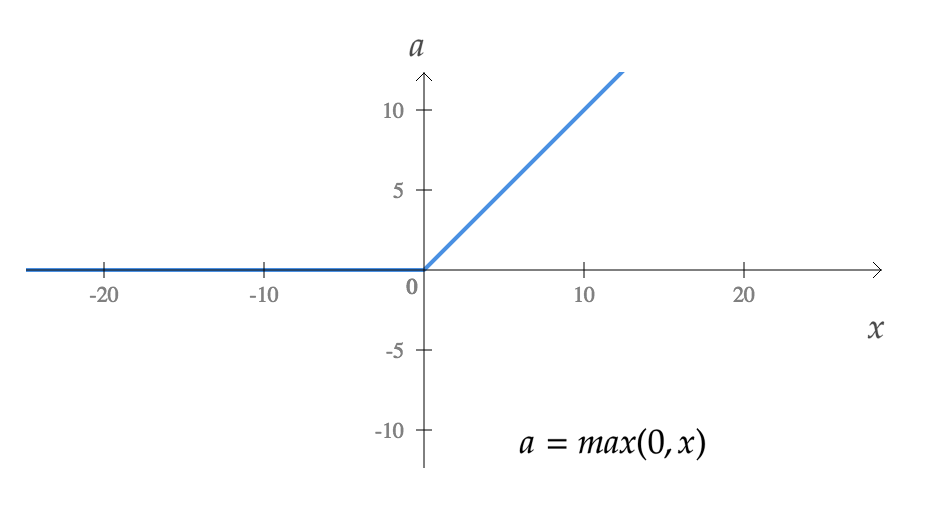
\includegraphics[width=0.45\linewidth , height=0.33\linewidth]{images/relu.png}}
\subcaptionbox{\label{sfig:sigmoid}}{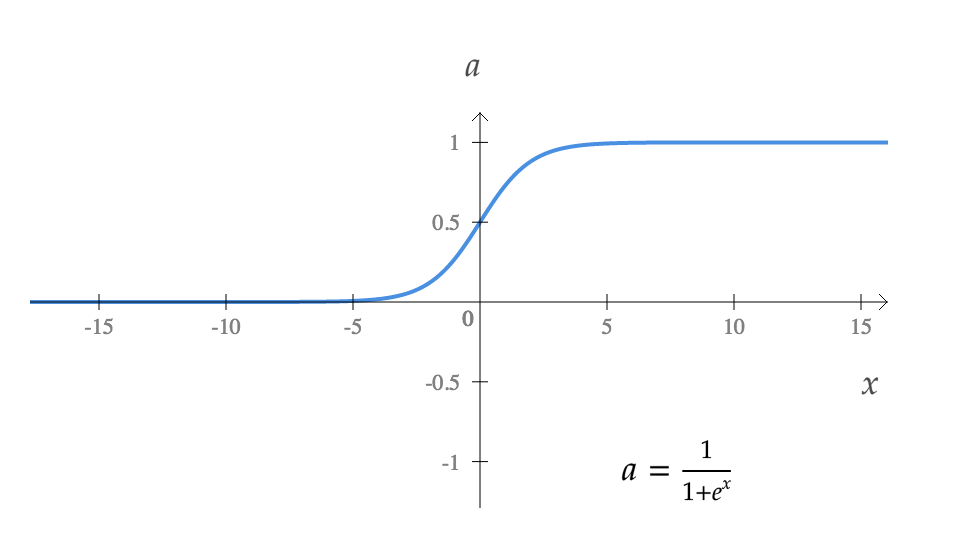
\includegraphics[width=0.45\linewidth , height=0.33\linewidth]{images/sigmoid.png}}
\caption{Common choices of activation functions are ~\subref{sfig:relu} Relu function $a=\mathrm{max}(0,x)$, which cuts values below zero and ~\subref{sfig:sigmoid} Sigmoid function $a=\frac{1}{1+e^{x}}$, which forces the values to be between zero and one.}
\label{fig:activation}
\end{figure}
%%%%%%%%%%%%%%%%%%%%%%%%%%%%%%%%%%%%%%%%%%%%%%%%%%%%%%%%%%%%
\subsection{Training neural networks}
Consider the output $\hat { y } $ as the prediction of our network for some task. In a supervised learning problem, the aim is to reduce the error between the prediction ($\hat { y } $) and the true label $y$. As a result, a cost function can be defined as $J$ in Equation~\ref{eq:cost_nn}, where $L$ denotes the loss function on a single training example and $m$ is the size of the training set. The \emph{cost function} is simply the sum of all losses on the training set.
% BR: you should briefly mention what types of loss functions exist, or
% use a simple one (MSE or something?)
\begin{equation}
J(\theta,b)=\sum _{ j=1 }^{ m }{ L( } \hat { y }^{ (i) } ,y^{ (i) })
\label{eq:cost_nn}
\end{equation}
The loss for a single input is computed by the \emph{loss function} $L$ and the sum of loses for all inputs is computed by the cost function $J$. There exists various loss functions, which are chosen based on the problem at hand. We introduce three of the most commonly used functions, which are used by the models in this thesis: \\
\begin{inparaenum}
\item \emph{Mean Squared Error} (MSE) or \emph{quadratic cost} minimizes the quadratic sum of distances between true label of each data point $y^{ (i) }$ and it's prediction $\hat { y } ^{ (i) }$~\brackettext{\cite{DBLP:reference/ml/2017}}: 
\begin{equation}
L=\frac { 1 }{ n } \sum _{ i=1 }^{ n }{ (\hat { y } ^{ (i) }- } y^{ (i) })^{ 2 }
\end{equation}
\item \emph{Kullback Leibler (KL) Divergence} also known as relative entropy, is a measure of how one probability distribution $y^{ (i) }$ (predicted distribution) diverges from a second probability distribution $\hat { y } ^{ (i) }$ (true distribution), the higher is the KL divergence, the more different the are distributions. KL divergence is not symmetric: The KL from $y^{ (i) }$ to $\hat { y } ^{ (i) }$ is generally not the same as the KL from $\hat { y } ^{ (i) }$ to $y^{ (i) }$~\brackettext{\cite{DBLP:books/daglib/0016881}}. The formula consists of two parts, where the first part is called \emph{entropy} and the second part \emph{cross-entropy}.
\begin{equation}
\begin{split}
L=\frac { 1 }{ n } \sum _{ i=1 }^{ n }{ D_{ kl }(y^{ (i) }||\hat { y } ^{ (i) }) } =\\
 \frac { 1 }{ n } \sum _{ i=1 }^{ n }{ (y^{ (i) }\log{(\frac { y^{ (i) } }{ \hat { y } ^{ (i) } } )) }} =\\
 \underbrace { \frac { 1 }{ n } \sum _{ i=1 }^{ n }{ (y^{ (i) }\log{(y^{ (i) })) }} - }_{ entropy } \underbrace { \frac { 1 }{ n } \sum _{ i=1 }^{ n }{ (y^{ (i) }\log{(\hat { y } ^{ (i) })) }}  }_{ cross-entropy } 
 \end{split}
\end{equation}
\item \emph{Cross Entropy} is commonly-used where labels are assumed to take only two values and corresponds to the second part of KL divergence formula, where the second distribution $\hat { y } ^{ (i) }$ is fixed~\brackettext{\cite{DBLP:books/daglib/0016881}}. The cross entropy for a classification problem with two classes is defined as:  
\begin{equation}
L=-\frac { 1 }{ n } \sum _{ i=1 }^{ n }{ [y^{ (i) }\log{(\hat { y } ^{ (i) })+(1-  y^{ (i) }}})\log{(1-\hat { y } ^{ (i) }})
\end{equation}
\end{inparaenum}
The goal of the training phase is to learn a weight matrix $\Theta$ and a bias term $b$ such that the overall cost is minimized. This naturally leads to an optimization problem, which is  typically solved using \emph{Gradient Descent} (GD)~\brackettext{\cite{DBLP:journals/corr/Ruder16}}.
Gradient descent is a way to minimize an objective function by finding local minima based on local gradients.
% BR: I slightly object to that description. I would drop the
% 'parameterized ...' part and just leave it as 'a way to minimize an
% objective function by finding local minima based on local gradients'
% or something like that.
It is an iterative algorithm, where in each step parameters of the model are updated using the gradient of the function. A single step of GD  for one parameter $\theta$ can be seen in Equation~\ref{eq:gd}, where the previous value of the parameter is updated based on the gradient of the cost function in respect with $\theta$. Here, $\alpha$ is the \emph{learning rate} or the step size and controls the magnitude of the update in each iteration. 
\begin{equation}
\theta=: \theta- \alpha\frac { \partial J(\theta) }{ \partial \theta }
\label{eq:gd}
\end{equation}
In a dataset with $m$ training examples, for each training example, the gradient of the cost function with respect to every weight and bias has to be calculated and accumulated.
After iterating through all the training examples the weights and bias terms will be updated by the accumulate sum. This process is repeated for some number of iterations, where each iteration is one pass through the training set. Because the number of training examples for deep learning models are usually large, variations of GD have been introduce to speed up the process, three main type of GD are as follows: 
\begin{itemize}
\item \textbf{Mini-batch GD:} Instead of iterating over all training examples, a subset of a batch, i.e.,\ a subset of the input data, is considered, before making an update. This is a good choice for very large datasets.
\item \textbf{Stochastic-GD:} In this case, only one example is looked at, before making an update. 
\item \textbf{Batch-GD:} The original algorithm with iteration over all examples. 
% BR: It's inconsistent to refer to it as a variation of the algorithm,
% though, right?
\end{itemize} 
Considering the most simple case (a function with only one parameter) gradient descent is illustrated in Figure~\ref{fig:gradientD}. As shown in the figure, the derivative or the slope of the function is positive on the right side of the minimum (the update rule will decrease $\theta$) and negative on the left size (the update rule will increase $\theta$). The same rule holds in higher dimensions as well. Although the figure illustrates a function with global minimum, it is worth noting that GD is not guaranteed to find the global minimum and is often stuck in local minima.\\
% BR: This is very nice. To be mathematically airtight, you could write
% that this holds in higher dimensions as well. However, one may require
% approximations of the gradient there, of course.
%
%\begin{algorithm}[htbp]
%  %
%  \begin{algorithmic}[1]
%    \newcommand{\UF}{\mathrm{U}}
%   \While{(not converged)}
% \State $\theta=: \theta- \alpha\frac { \partial J(\theta) }{ \partial \theta } $
%  \EndWhile
%  \end{algorithmic}
%  %
%\caption{: Gradient decent}
% \label{algo:gd}
%\end{algorithm}

\begin{figure}
\centering 
\resizebox{0.65\textwidth}{0.4\textwidth}{      
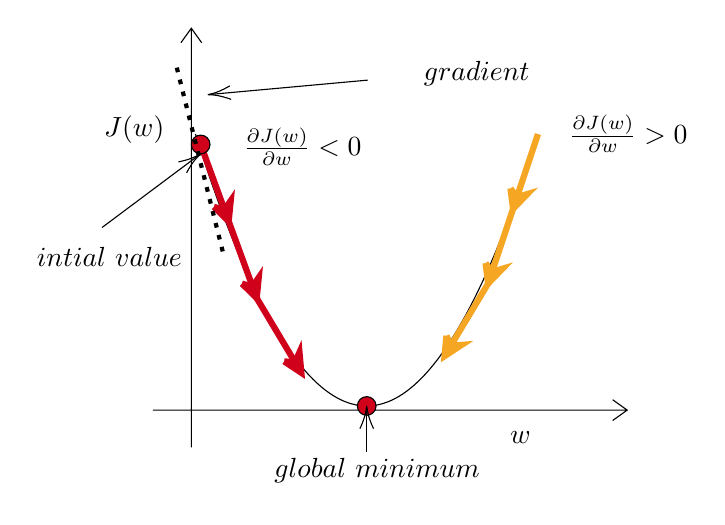
\begin{tikzpicture}[x=0.75pt,y=0.75pt,yscale=-1,xscale=1]
%uncomment if require: \path (0,300); %set diagram left start at 0, and has height of 300

\draw  (75,190) -- (303.5,190)(93.5,6) -- (93.5,208) (296.5,185) -- (303.5,190) -- (296.5,195) (88.5,13) -- (93.5,6) -- (98.5,13)  ;
\draw   (95.5,57) .. controls (150.5,231.67) and (205.5,231.67) .. (260.5,57) ;
\draw [color={rgb, 255:red, 208; green, 2; blue, 27 }  ,draw opacity=1 ][line width=2.25]    (98,62) -- (111.5,99) ;
\draw [shift={(111.5,99)}, rotate = 249.95] [color={rgb, 255:red, 208; green, 2; blue, 27 }  ,draw opacity=1 ][fill={rgb, 255:red, 208; green, 2; blue, 27 }  ,fill opacity=1 ][line width=2.25]   (8.93,-4.29) -- (0,0) -- (8.93,4.29) -- (5.93,0) -- (8.93,-4.29)    ;

\draw [color={rgb, 255:red, 208; green, 2; blue, 27 }  ,draw opacity=1 ][line width=2.25]    (111.5,99) -- (125,136) ;
\draw [shift={(125,136)}, rotate = 249.95] [color={rgb, 255:red, 208; green, 2; blue, 27 }  ,draw opacity=1 ][fill={rgb, 255:red, 208; green, 2; blue, 27 }  ,fill opacity=1 ][line width=2.25]   (8.93,-4.29) -- (0,0) -- (8.93,4.29) -- (5.93,0) -- (8.93,-4.29)    ;

\draw [color={rgb, 255:red, 208; green, 2; blue, 27 }  ,draw opacity=1 ][line width=2.25]    (125,136) -- (146.5,172) ;
\draw [shift={(146.5,172)}, rotate = 239.15] [color={rgb, 255:red, 208; green, 2; blue, 27 }  ,draw opacity=1 ][fill={rgb, 255:red, 208; green, 2; blue, 27 }  ,fill opacity=1 ][line width=2.25]   (8.93,-4.29) -- (0,0) -- (8.93,4.29) -- (5.93,0) -- (8.93,-4.29)    ;

\draw [color={rgb, 255:red, 245; green, 166; blue, 35 }  ,draw opacity=1 ][line width=2.25]    (260.5,57) -- (248.5,93) ;
\draw [shift={(248.5,93)}, rotate = 288.43] [color={rgb, 255:red, 245; green, 166; blue, 35 }  ,draw opacity=1 ][fill={rgb, 255:red, 245; green, 166; blue, 35 }  ,fill opacity=1 ][line width=2.25]   (8.93,-4.29) -- (0,0) -- (8.93,4.29) -- (5.93,0) -- (8.93,-4.29)    ;

\draw [color={rgb, 255:red, 245; green, 166; blue, 35 }  ,draw opacity=1 ][line width=2.25]    (248.5,93) -- (236.5,129) ;
\draw [shift={(236.5,129)}, rotate = 288.43] [color={rgb, 255:red, 245; green, 166; blue, 35 }  ,draw opacity=1 ][fill={rgb, 255:red, 245; green, 166; blue, 35 }  ,fill opacity=1 ][line width=2.25]   (8.93,-4.29) -- (0,0) -- (8.93,4.29) -- (5.93,0) -- (8.93,-4.29)    ;

\draw [color={rgb, 255:red, 245; green, 166; blue, 35 }  ,draw opacity=1 ][line width=2.25]    (236.5,129) -- (215.5,164) ;
\draw [shift={(215.5,164)}, rotate = 300.96] [color={rgb, 255:red, 245; green, 166; blue, 35 }  ,draw opacity=1 ][fill={rgb, 255:red, 245; green, 166; blue, 35 }  ,fill opacity=1 ][line width=2.25]   (8.93,-4.29) -- (0,0) -- (8.93,4.29) -- (5.93,0) -- (8.93,-4.29)    ;

\draw  [fill={rgb, 255:red, 208; green, 2; blue, 27 }  ,fill opacity=1 ]  (98, 62) circle [x radius= 4.5, y radius= 4.5]  ;
\draw    (50.5,102) -- (98,66.5) ;
\draw [shift={(98,66.5)}, rotate = 503.23] [color={rgb, 255:red, 0; green, 0; blue, 0 }  ]   (0,0) .. controls (3.31,-0.3) and (6.95,-1.4) .. (10.93,-3.29)(0,0) .. controls (3.31,0.3) and (6.95,1.4) .. (10.93,3.29)   ;

\draw  [fill={rgb, 255:red, 208; green, 2; blue, 27 }  ,fill opacity=1 ]  (178, 188) circle [x radius= 4.5, y radius= 4.5]  ;
\draw    (178,210) -- (178,188) ;
\draw [shift={(178,188)}, rotate = 450] [color={rgb, 255:red, 0; green, 0; blue, 0 }  ]   (0,0) .. controls (3.31,-0.3) and (6.95,-1.4) .. (10.93,-3.29)(0,0) .. controls (3.31,0.3) and (6.95,1.4) .. (10.93,3.29)   ;

\draw [line width=1.5]  [dash pattern={on 1.69pt off 2.76pt}]  (86.5,25) -- (109.5,117) ;


\draw    (178.5,31) -- (101.5,38) ;
\draw [shift={(101.5,38)}, rotate = 354.81] [color={rgb, 255:red, 0; green, 0; blue, 0 }  ]   (0,0) .. controls (3.31,-0.3) and (6.95,-1.4) .. (10.93,-3.29)(0,0) .. controls (3.31,0.3) and (6.95,1.4) .. (10.93,3.29)   ;


\draw (252,203) node   {$w$};
\draw (66,55) node   {$J( w)$};
\draw (147,63) node   {$\frac{\partial J( w)}{\partial w} < 0$};
\draw (304,57) node   {$\frac{\partial J( w)}{\partial w}  >0$};
\draw (183,219) node   {$global\ minimum$};
\draw (54,116) node   {$intial\ value$};
\draw (231,28) node   {$gradient$};


\end{tikzpicture}

}
\caption{Gradient decent on a one-dimensional function with only one parameter.
In each iteration, we take a step in the direction of the gradient. The gradient will guide the algorithm to the functions local minimum.
% BR: do you want to mention getting stuck in local optima?
}
\label{fig:gradientD}
\end{figure}
\noindent
%%%%%%%%%%%%%%%%%%%%%%%%%%%%%%%%%%%%%%%%%%%%%%%%%%%%%%%%%%%%
\subsection{Embeddings}\label{subsec:embeddings}
One of the challenges of machine learning is to come up with suitable features for algorithms. These features often have to be task-specific and reflect the needs of the downstream tasks, for example, a task that uses embeddings as input features. \emph{Representation learning} attempts to learn good features and representations automatically~\brackettext{\cite{SCHOL:journals/FDS/ZhongWD16}}. \emph{Principle Component Analysis} (PCA)~\brackettext{\cite{DBLP:journals/corr/Shlens14}} is one example of a traditional method for representation learning from high dimensional data. More recently, neural networks are used to obtain these low-dimensional representations. In a deep learning architecture, the output of each intermediate layer can be viewed as a representation of the original input data. Each unit inn the hidden layer of the network computes a non-linear combination of the inputs that is used by the next layer.  If the dimension of the hidden layer is much smaller than the input layer, a low-dimensional representation of the data is learned in the hidden layer. Based on this principle almost any type of data (e.g., images, sounds and text) can be transformed into embeddings with lower dimensions. In this work, we focus on learning low-dimensional representation for two types of data structures, namely, for words (\emph{word embeddings}) and for graphs (\emph{graph embeddings}). \\
Text is inherently high-dimensional, requiring a specific form of embedding.
% BR: The sentence is a little bit too short and disrupts the flow.
% Maybe: 'However, text is inherently high-dimensional, requiring
% a specific form of embedding'.
In most traditional NLP systems, each word is represented as a one-hot vector of the size of the vocabulary, which is a high-dimensional, highly sparse vector. 
By feeding these high-dimensional representations to a neural network with a smaller hidden layer, a new representation (usually in the order of $100$ dimensions) for each word is learned, which is a more dense vector representation for each word. For this purpose, different models have been proposed, the most famous being word2vec~\brackettext{\cite{DBLP:journals/corr/abs-1301-3781}}, which will be discussed in Section~\ref{sec:wordembeddig} in detail. All the models follow the same principle, which is illustrated in Figure~\ref{fig:emb}, where the one-hot vectors of words in the vocabulary are the input of the network and a low-dimensional hidden layer is responsible for encoding the representation of input words.  The size of the output layer depends on the particular architecture and the cost function. In addition, the network can be composed of multiple layers, but for our purposes, we focus on shallow networks with only one hidden layer. \\
\begin{figure}
\centering 
\resizebox{0.8\textwidth}{0.48\textwidth}{      
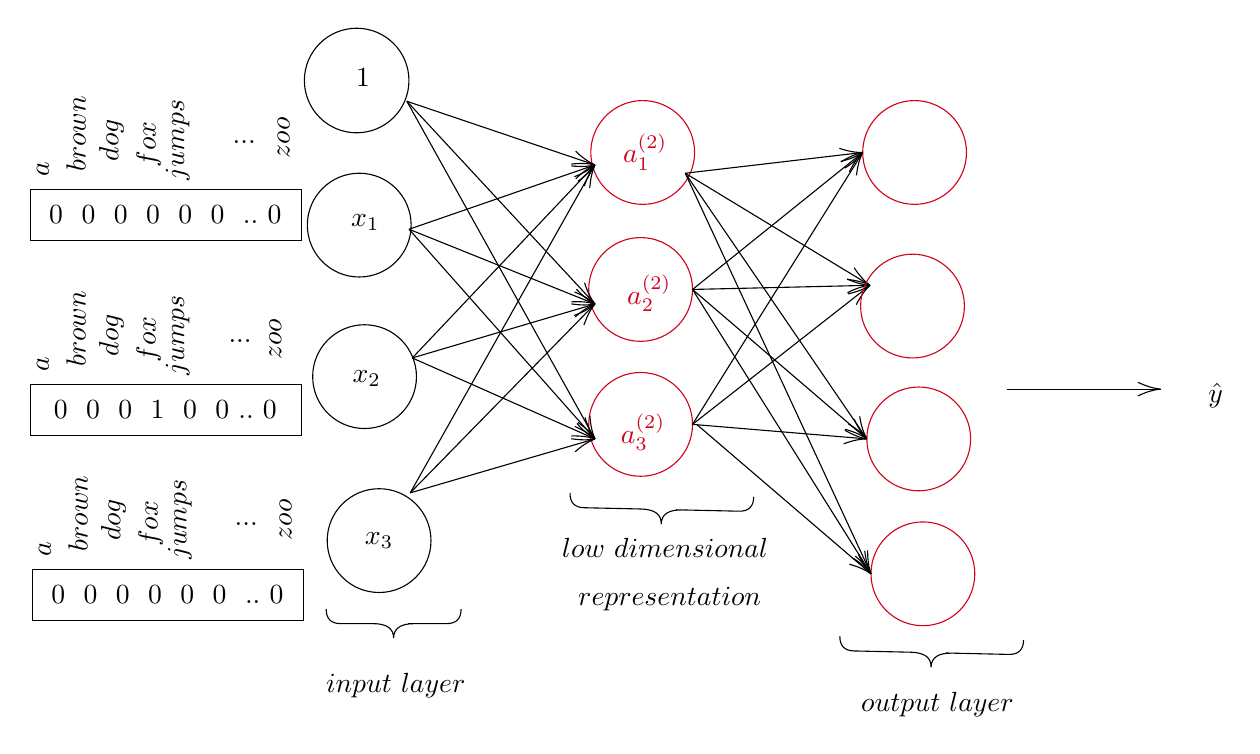
\begin{tikzpicture}[x=0.75pt,y=0.75pt,yscale=-1,xscale=1]
%uncomment if require: \path (0,406); %set diagram left start at 0, and has height of 406

\draw  [color={rgb, 255:red, 208; green, 2; blue, 27 }  ,draw opacity=1 ]  (302, 69) circle [x radius= 25, y radius= 25]  ;
\draw  [color={rgb, 255:red, 208; green, 2; blue, 27 }  ,draw opacity=1 ]  (301, 135) circle [x radius= 25, y radius= 25]  ;
\draw  [color={rgb, 255:red, 208; green, 2; blue, 27 }  ,draw opacity=1 ]  (301, 200) circle [x radius= 25, y radius= 25]  ;
\draw    (322.5,79) -- (411.5,133) ;
\draw [shift={(411.5,133)}, rotate = 211.25] [color={rgb, 255:red, 0; green, 0; blue, 0 }  ]   (0,0) .. controls (3.31,-0.3) and (6.95,-1.4) .. (10.93,-3.29)(0,0) .. controls (3.31,0.3) and (6.95,1.4) .. (10.93,3.29)   ;

\draw    (326,135) -- (411.5,133) ;
\draw [shift={(411.5,133)}, rotate = 538.6600000000001] [color={rgb, 255:red, 0; green, 0; blue, 0 }  ]   (0,0) .. controls (3.31,-0.3) and (6.95,-1.4) .. (10.93,-3.29)(0,0) .. controls (3.31,0.3) and (6.95,1.4) .. (10.93,3.29)   ;

\draw    (326,200) -- (411.5,133) ;
\draw [shift={(411.5,133)}, rotate = 501.92] [color={rgb, 255:red, 0; green, 0; blue, 0 }  ]   (0,0) .. controls (3.31,-0.3) and (6.95,-1.4) .. (10.93,-3.29)(0,0) .. controls (3.31,0.3) and (6.95,1.4) .. (10.93,3.29)   ;

\draw  [color={rgb, 255:red, 208; green, 2; blue, 27 }  ,draw opacity=1 ]  (433, 69) circle [x radius= 25, y radius= 25]  ;
\draw    (477.5,183) -- (551.5,183) ;
\draw [shift={(551.5,183)}, rotate = 180] [color={rgb, 255:red, 0; green, 0; blue, 0 }  ]   (0,0) .. controls (3.31,-0.3) and (6.95,-1.4) .. (10.93,-3.29)(0,0) .. controls (3.31,0.3) and (6.95,1.4) .. (10.93,3.29)   ;

\draw    (165.43, 104) circle [x radius= 25, y radius= 25]  ;
\draw    (168, 177) circle [x radius= 25, y radius= 25]  ;
\draw    (175, 256) circle [x radius= 25, y radius= 25]  ;
\draw    (164.19, 34.33) circle [x radius= 25.19, y radius= 25.19]  ;
\draw    (188.38,44.33) -- (279,75) ;
\draw [shift={(279,75)}, rotate = 198.7] [color={rgb, 255:red, 0; green, 0; blue, 0 }  ]   (0,0) .. controls (3.31,-0.3) and (6.95,-1.4) .. (10.93,-3.29)(0,0) .. controls (3.31,0.3) and (6.95,1.4) .. (10.93,3.29)   ;

\draw    (188.38,44.33) -- (279,142) ;
\draw [shift={(279,142)}, rotate = 227.14] [color={rgb, 255:red, 0; green, 0; blue, 0 }  ]   (0,0) .. controls (3.31,-0.3) and (6.95,-1.4) .. (10.93,-3.29)(0,0) .. controls (3.31,0.3) and (6.95,1.4) .. (10.93,3.29)   ;

\draw    (188.38,44.33) -- (279,207) ;
\draw [shift={(279,207)}, rotate = 240.88] [color={rgb, 255:red, 0; green, 0; blue, 0 }  ]   (0,0) .. controls (3.31,-0.3) and (6.95,-1.4) .. (10.93,-3.29)(0,0) .. controls (3.31,0.3) and (6.95,1.4) .. (10.93,3.29)   ;

\draw    (189.43,106) -- (279,207) ;
\draw [shift={(279,207)}, rotate = 228.43] [color={rgb, 255:red, 0; green, 0; blue, 0 }  ]   (0,0) .. controls (3.31,-0.3) and (6.95,-1.4) .. (10.93,-3.29)(0,0) .. controls (3.31,0.3) and (6.95,1.4) .. (10.93,3.29)   ;

\draw    (189.43,106) -- (279,142) ;
\draw [shift={(279,142)}, rotate = 201.9] [color={rgb, 255:red, 0; green, 0; blue, 0 }  ]   (0,0) .. controls (3.31,-0.3) and (6.95,-1.4) .. (10.93,-3.29)(0,0) .. controls (3.31,0.3) and (6.95,1.4) .. (10.93,3.29)   ;

\draw    (189.43,106) -- (279,75) ;
\draw [shift={(279,75)}, rotate = 520.9100000000001] [color={rgb, 255:red, 0; green, 0; blue, 0 }  ]   (0,0) .. controls (3.31,-0.3) and (6.95,-1.4) .. (10.93,-3.29)(0,0) .. controls (3.31,0.3) and (6.95,1.4) .. (10.93,3.29)   ;

\draw    (191,168) -- (279,75) ;
\draw [shift={(279,75)}, rotate = 493.42] [color={rgb, 255:red, 0; green, 0; blue, 0 }  ]   (0,0) .. controls (3.31,-0.3) and (6.95,-1.4) .. (10.93,-3.29)(0,0) .. controls (3.31,0.3) and (6.95,1.4) .. (10.93,3.29)   ;

\draw    (191,168) -- (279,142) ;
\draw [shift={(279,142)}, rotate = 523.54] [color={rgb, 255:red, 0; green, 0; blue, 0 }  ]   (0,0) .. controls (3.31,-0.3) and (6.95,-1.4) .. (10.93,-3.29)(0,0) .. controls (3.31,0.3) and (6.95,1.4) .. (10.93,3.29)   ;

\draw    (191,168) -- (279,207) ;
\draw [shift={(279,207)}, rotate = 203.9] [color={rgb, 255:red, 0; green, 0; blue, 0 }  ]   (0,0) .. controls (3.31,-0.3) and (6.95,-1.4) .. (10.93,-3.29)(0,0) .. controls (3.31,0.3) and (6.95,1.4) .. (10.93,3.29)   ;

\draw    (190,233) -- (279,75) ;
\draw [shift={(279,75)}, rotate = 479.39] [color={rgb, 255:red, 0; green, 0; blue, 0 }  ]   (0,0) .. controls (3.31,-0.3) and (6.95,-1.4) .. (10.93,-3.29)(0,0) .. controls (3.31,0.3) and (6.95,1.4) .. (10.93,3.29)   ;

\draw    (190,233) -- (279,142) ;
\draw [shift={(279,142)}, rotate = 494.36] [color={rgb, 255:red, 0; green, 0; blue, 0 }  ]   (0,0) .. controls (3.31,-0.3) and (6.95,-1.4) .. (10.93,-3.29)(0,0) .. controls (3.31,0.3) and (6.95,1.4) .. (10.93,3.29)   ;

\draw    (190,233) -- (279,207) ;
\draw [shift={(279,207)}, rotate = 523.72] [color={rgb, 255:red, 0; green, 0; blue, 0 }  ]   (0,0) .. controls (3.31,-0.3) and (6.95,-1.4) .. (10.93,-3.29)(0,0) .. controls (3.31,0.3) and (6.95,1.4) .. (10.93,3.29)   ;

\draw   (149.5,289) .. controls (149.5,293.67) and (151.83,296) .. (156.5,296) -- (172,296) .. controls (178.67,296) and (182,298.33) .. (182,303) .. controls (182,298.33) and (185.33,296) .. (192,296)(189,296) -- (207.5,296) .. controls (212.17,296) and (214.5,293.67) .. (214.5,289) ;
\draw   (267,233) .. controls (266.89,237.67) and (269.17,240.05) .. (273.84,240.16) -- (301.1,240.77) .. controls (307.76,240.92) and (311.04,243.32) .. (310.93,247.99) .. controls (311.04,243.32) and (314.42,241.07) .. (321.09,241.22)(318.09,241.15) -- (348.34,241.83) .. controls (353.01,241.94) and (355.39,239.66) .. (355.5,234.99) ;
\draw   (397,302) .. controls (396.89,306.67) and (399.17,309.05) .. (403.84,309.16) -- (431.1,309.77) .. controls (437.76,309.92) and (441.04,312.32) .. (440.93,316.99) .. controls (441.04,312.32) and (444.42,310.07) .. (451.09,310.22)(448.09,310.15) -- (478.34,310.83) .. controls (483.01,310.94) and (485.39,308.66) .. (485.5,303.99) ;
\draw    (7, 87) rectangle (137.5, 111.33)   ;
\draw    (7, 181) rectangle (137.5, 205.33)   ;
\draw    (8, 270) rectangle (138.5, 294.33)   ;
\draw  [color={rgb, 255:red, 208; green, 2; blue, 27 }  ,draw opacity=1 ]  (432, 143) circle [x radius= 25, y radius= 25]  ;
\draw  [color={rgb, 255:red, 208; green, 2; blue, 27 }  ,draw opacity=1 ]  (435, 207) circle [x radius= 25, y radius= 25]  ;
\draw  [color={rgb, 255:red, 208; green, 2; blue, 27 }  ,draw opacity=1 ]  (437, 272) circle [x radius= 25, y radius= 25]  ;
\draw    (326,135) -- (410,207) ;
\draw [shift={(410,207)}, rotate = 220.6] [color={rgb, 255:red, 0; green, 0; blue, 0 }  ]   (0,0) .. controls (3.31,-0.3) and (6.95,-1.4) .. (10.93,-3.29)(0,0) .. controls (3.31,0.3) and (6.95,1.4) .. (10.93,3.29)   ;

\draw    (322.5,79) -- (408,69) ;
\draw [shift={(408,69)}, rotate = 533.3299999999999] [color={rgb, 255:red, 0; green, 0; blue, 0 }  ]   (0,0) .. controls (3.31,-0.3) and (6.95,-1.4) .. (10.93,-3.29)(0,0) .. controls (3.31,0.3) and (6.95,1.4) .. (10.93,3.29)   ;

\draw    (322.5,79) -- (410,207) ;
\draw [shift={(410,207)}, rotate = 235.64] [color={rgb, 255:red, 0; green, 0; blue, 0 }  ]   (0,0) .. controls (3.31,-0.3) and (6.95,-1.4) .. (10.93,-3.29)(0,0) .. controls (3.31,0.3) and (6.95,1.4) .. (10.93,3.29)   ;

\draw    (322.5,79) -- (412,272) ;
\draw [shift={(412,272)}, rotate = 245.12] [color={rgb, 255:red, 0; green, 0; blue, 0 }  ]   (0,0) .. controls (3.31,-0.3) and (6.95,-1.4) .. (10.93,-3.29)(0,0) .. controls (3.31,0.3) and (6.95,1.4) .. (10.93,3.29)   ;

\draw    (326,135) -- (408,69) ;
\draw [shift={(408,69)}, rotate = 501.17] [color={rgb, 255:red, 0; green, 0; blue, 0 }  ]   (0,0) .. controls (3.31,-0.3) and (6.95,-1.4) .. (10.93,-3.29)(0,0) .. controls (3.31,0.3) and (6.95,1.4) .. (10.93,3.29)   ;

\draw    (326,200) -- (410,207) ;
\draw [shift={(410,207)}, rotate = 184.76] [color={rgb, 255:red, 0; green, 0; blue, 0 }  ]   (0,0) .. controls (3.31,-0.3) and (6.95,-1.4) .. (10.93,-3.29)(0,0) .. controls (3.31,0.3) and (6.95,1.4) .. (10.93,3.29)   ;

\draw    (326,200) -- (408,69) ;
\draw [shift={(408,69)}, rotate = 482.04] [color={rgb, 255:red, 0; green, 0; blue, 0 }  ]   (0,0) .. controls (3.31,-0.3) and (6.95,-1.4) .. (10.93,-3.29)(0,0) .. controls (3.31,0.3) and (6.95,1.4) .. (10.93,3.29)   ;

\draw    (328,200) -- (412,272) ;
\draw [shift={(412,272)}, rotate = 220.6] [color={rgb, 255:red, 0; green, 0; blue, 0 }  ]   (0,0) .. controls (3.31,-0.3) and (6.95,-1.4) .. (10.93,-3.29)(0,0) .. controls (3.31,0.3) and (6.95,1.4) .. (10.93,3.29)   ;

\draw    (326,135) -- (412,272) ;
\draw [shift={(412,272)}, rotate = 237.88] [color={rgb, 255:red, 0; green, 0; blue, 0 }  ]   (0,0) .. controls (3.31,-0.3) and (6.95,-1.4) .. (10.93,-3.29)(0,0) .. controls (3.31,0.3) and (6.95,1.4) .. (10.93,3.29)   ;


\draw (303.21,68.84) node [color={rgb, 255:red, 208; green, 2; blue, 27 }  ,opacity=1 ]  {$a^{( 2)}_{1}$};
\draw (305.21,136.84) node [color={rgb, 255:red, 208; green, 2; blue, 27 }  ,opacity=1 ]  {$a^{( 2)}_{2}$};
\draw (302.21,203.84) node [color={rgb, 255:red, 208; green, 2; blue, 27 }  ,opacity=1 ]  {$a^{( 2)}_{3}$};
\draw (169,178) node   {$x_{2}$};
\draw (168.37,102.96) node   {$x_{1}$};
\draw (175,256) node   {$x_{3}$};
\draw (167.21,32.84) node   {$1$};
\draw (578,186) node   {$\hat{y}$};
\draw (183,326) node   {$input\ layer$};
\draw (315,272) node   {$ \begin{gathered}
low\ dimensional\ \\
representation
\end{gathered}$};
\draw (444,335) node   {$output\ layer$};
\draw (72,99) node   {$0\ \ 0\ \ 0\ \ 0\ \ 0\ \ 0\ \ ..\ 0$};
\draw (13,77) node [rotate=-270]  {$a$};
\draw (29,60) node [rotate=-270]  {$brown$};
\draw (46,63) node [rotate=-270]  {$dog$};
\draw (78,63) node [rotate=-270]  {$jumps$};
\draw (129,62) node [rotate=-270]  {$zoo$};
\draw (64,65) node [rotate=-270]  {$fox$};
\draw (72,193) node   {$0\ \ 0\ \ 0\ \ 1\ \ 0\ \ 0\ ..\ 0$};
\draw (13,171) node [rotate=-270]  {$a$};
\draw (29,154) node [rotate=-270]  {$brown$};
\draw (46,157) node [rotate=-270]  {$dog$};
\draw (78,157) node [rotate=-270]  {$jumps$};
\draw (64,159) node [rotate=-270]  {$fox$};
\draw (73,282) node   {$0\ \ 0\ \ 0\ \ 0\ \ 0\ \ 0\ \ ..\ 0$};
\draw (14,260) node [rotate=-270]  {$a$};
\draw (30,243) node [rotate=-270]  {$brown$};
\draw (47,246) node [rotate=-270]  {$dog$};
\draw (79,246) node [rotate=-270]  {$jumps$};
\draw (65,248) node [rotate=-270]  {$fox$};
\draw (125,159) node [rotate=-270]  {$zoo$};
\draw (130,246) node [rotate=-270]  {$zoo$};
\draw (110,64) node   {$...$};
\draw (108,160) node   {$...$};
\draw (111,248) node   {$...$};


\end{tikzpicture}

}
\caption{Underlying principle of word embeddings. The high-dimensional one-hot vectors are the input of the network. The hidden layer learns a dense representation to either predict the surrounding words or to optimize a different cost function in the output layer.}
\label{fig:emb}
\end{figure}
\noindent
% BR: The change between these two sections is very abrupt.
Learning low-dimensional representation is not only a challenge for NLP, but extends to many domains, such as image and graph analysis. Graph embeddings, in particular,  aim to convert a graph with many edges and nodes into a low dimensional latent space while preserving the graph information~\brackettext{\cite{DBLP:journals/kbs/GoyalF18}}. One type of graph embedding is \emph{node embedding}, which represent each node of a graph as a vector in a low-dimensional space, where node proximity should be preserved in both spaces.
% BR: I would rather say that 'proximity should be preserved in both
% spaces'
The difference between various techniques lies in how they define \emph{``closeness''}~\brackettext{\cite{DBLP:journals/tkde/CaiZC18}}. For example, two nodes are considered close if they share the same neighbours or have a direct edge between them. In the next section, we will give a brief introduction to co-occurrence graphs, and in Section~\ref{sec:graph} the well-known graph embedding methods are explained.  

%%%%%%%%%%%%%%%%%%%%%%%%%%%%%%%%%%%%%%%%%%%%%%%%%%%%%%%%%%%%
\section{Co-occurrence Graphs}
\label{sec:graph}
Co-occurrence analysis, in terms of graphs, is not limited to text mining, but is a tool to find potential relationships between people, organizations, concepts, and biological organisms~\brackettext{\cite{SCHOL:journal/NAR/shiri}}. A word co-occurrence graph shows the word interactions in a corpus. A co-occurrence graph $G=(V,E)$ is defined by a set of all words $V$ as nodes and edges $E$ between them, where there is an edge based on their paired presence in a unit of text~\brackettext{\cite{DBLP:conf/cikm/RousseauV13,DBLP:journals/nle/NastaseMR15}}. If the entities in the text are annotated, the graph shows the positional relationship between entities and terms that occur in the text. There is an edge between two words, if they occur in the same sentence or paragraph~\brackettext{\cite{DBLP:conf/interspeech/YinBB18}}. If the graph is weighted, the edges indicate the strength of the connection between two words or entities, which related to the number of their co-occurrences or some kind of distance measure, e.g., number of tokens between them~\brackettext{\cite{SCHOL:book/mihalcea2011}}. Since these graphs encode all important words in the vocabulary, they can form a graph-based representation of the corpus, which we use instead of a textual corpus to generate embeddings, where relations between nearby words can be extracted based on edges and nearby nodes.\\

The \emph{LOAD model}~\brackettext{\cite{DBLP:conf/sigir/SpitzG16}} is an entity co-occurrence graph representation of large document collections. For each document, named entities from sentences are extracted and connected based on their distance in a graph structure. The original LOAD model contains node types of pages and sentences as well, which we disregard for our models, the entity types considered by the LOAD graph are actors, locations, organisation, dates, and terms.\\
The LOAD model encodes the strength of relationship between entities and terms in the edge weights. In most cases entities on the same page share some connection, regardless of their distance in the text, which the models that only look for relation in a single sentence often miss. The LOAD model proposes a sentence-based weighting function for capturing the relation between two entities, where the long-distance connections have lower weights. Equation~\ref{eq:load_dist} shows the weighting of a single edge in the LOAD model between two entities $v$ and $s$, where $\delta $ is a distance function. For entities other than terms, $\delta $ equals the number of sentences between the instances, or $0$ if they occur in the same sentence.
If $i$ and $ j$ do not occur on the same document: $ \delta(i, j) := \infty$. $ I_{ v }$ and $I_{ s } $ are the set of all occurrences of $v$ and $s$ in the document. $\exp$ forces the weight to diminish exponentially with the distance. Eventually, the sum of all these exponential distances creates the final weight.
\begin{equation}
e (v,s) :=\sum _{ i\in I_{ v } \\ j\in I_{ s } }^{  }{ \exp } (-\delta (i,j))
\label{eq:load_dist}
\end{equation}
The weights generated in this way encode the importance of one entity to another. The distance decays as the number of sentences between two entities grows. In addition, long-distance connections are considered very weak and are cut-off based on a threshold parameter. 
Despite the fact that related entities can be mentioned several sentences apart, terms are less likely to be related to entities outside of their own sentence, so the edges between terms and entities are limited to those that appear in the same sentence. ~\brackettext{\cite{DBLP:conf/sigir/SpitzG16}}. 
%%%%%%%%%%%%%%%%%%%%%%%%%%%%%%%%%%%%%%%%%%%%%%%%%%%%%%%%%%%%
\section{Word Embeddings}
\label{sec:wordembeddig}
A word embedding is defined as a mapping $ V\rightarrow { R }^{ d }:v \rightarrow w $ that maps a word $v$ from a vocabulary $V$ to a vector  $w$  in an embedding space of dimensionality $d$ ~\brackettext{\cite{DBLP:conf/emnlp/SchnabelLMJ15}}. The first model to learn word embeddings as dense vector was presented by Bengio et al., in which a feature vector, much smaller than the size of the vocabulary, was used to express words using a probabilistic model~\brackettext{\cite{DBLP:conf/nips/BengioDV00}}. The work of Collobert et al. in $2011$ proved that the word representation could not only be achieved through probabilistic models, but that neural network architectures can also learn these internal representations from vast amounts of mostly unlabeled training data~\brackettext{\cite{DBLP:journals/jmlr/CollobertWBKKK11}}. However, it was not until the word2vec method~\brackettext{\cite{DBLP:journals/corr/abs-1301-3781}} that word embeddings became applicable to large corpora. 
Window-based models such as word2vec learn the embeddings in terms of a supervised learning task, where the objective is to predict a word's context given a center word in a fixed window. A noticeable disadvantage of these models is that they do not operate directly on the co-occurrence statistics of the corpus. Instead, they scan context windows across sentences, which fails to take advantage of the vast amount of repetition in the data. Regardless of the fact that many words co-occur multiple times, for multiple passes through the data, a window-based method has to parse the whole corpus several times. On the other hand, a co-occurrence matrix can capture this repetition in a compact way and hence, save time and computational power.  \\
In contrast, matrix factorization methods operate directly on the co-occurrence matrix and capture the full statistics. Before word2vec, similar embeddings were generated using \emph{Singular Value Decomposition}(SVD) on co-occurrence matrices and keeping the top \emph{k} dimensions. These methods were also able to capture many semantic and syntactic analogies~\brackettext{\cite{SCHOL:journals/acm/Rohde}}. In $2014$ Levy and Goldberg showed that implicitly factorizing a word-context matrix, whose cells are the \emph{Point wise Mutual Information} (PMI) of the respective word and context pairs, can generate embeddings close to word2vec\brackettext{\cite{DBLP:conf/nips/LevyG14}}.
The main disadvantage of count based methods is that they are computationally slow on large matrices. In addition, adding new words to the model is difficult, since it requires training a new model from the start.\\
The GloVe model~\brackettext{\cite{DBLP:conf/emnlp/PenningtonSM14}}  combines the matrix factorization for generating embeddings with window-based methods and uses the global statistics of the corpus or in another word the co-occurrence matrix to generate embeddings. In addition, unlike the word2vec model that scales with the size of the corpus, general statistics of the data has to be generated only once in terms of the co-occurrence matrix and then additional computations can be performed on the matrix alone.
\begin{figure}
\centering 
\resizebox{0.63\textwidth}{0.5\textwidth}{      
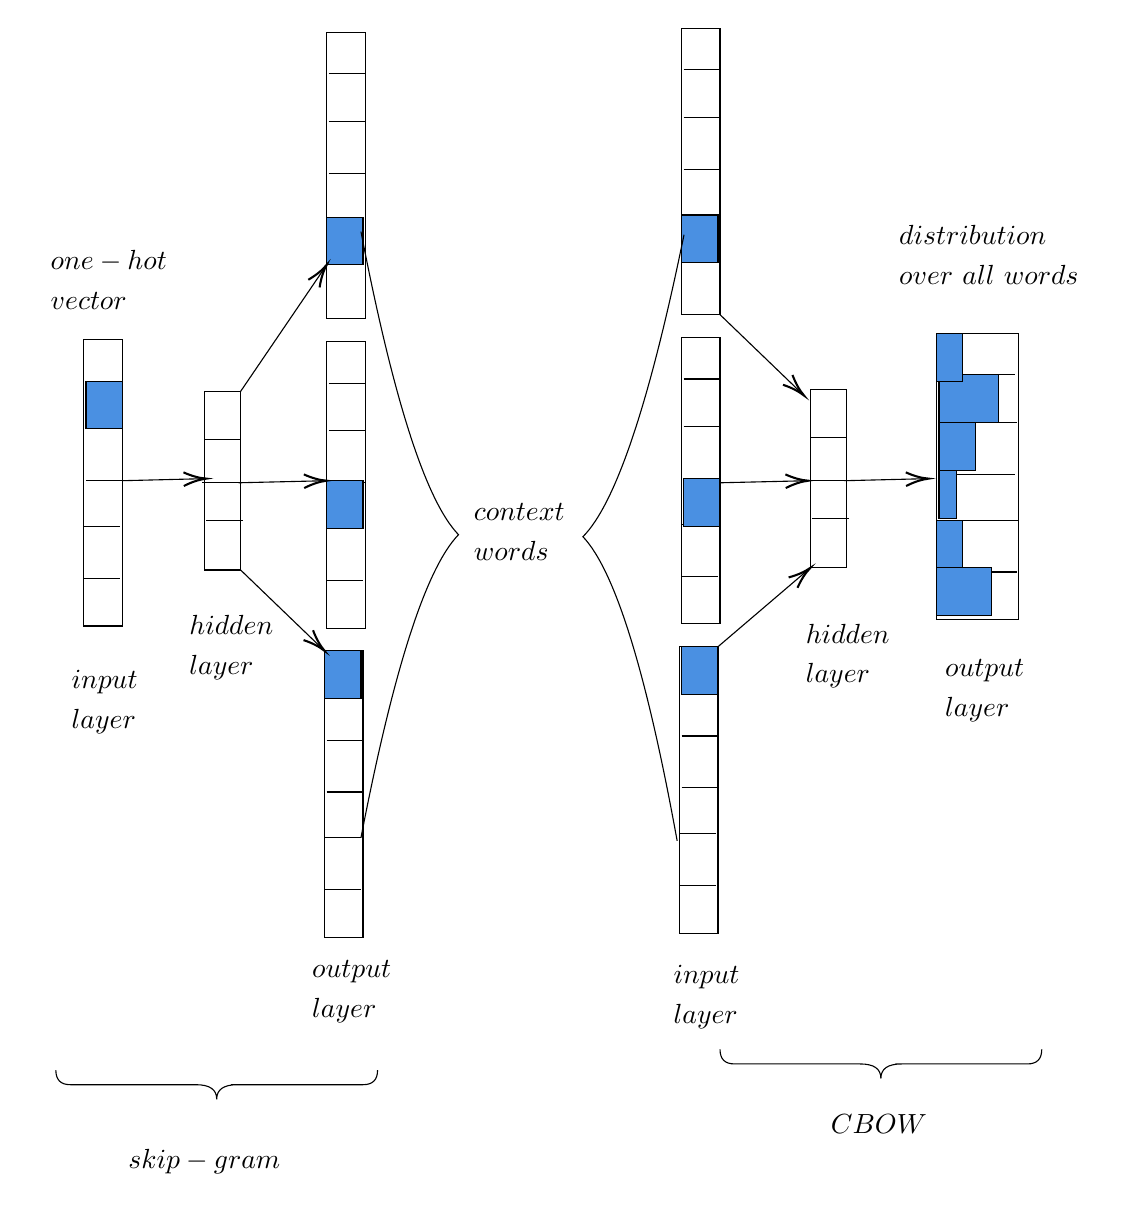
\begin{tikzpicture}[x=0.75pt,y=0.75pt,yscale=-1,xscale=1]
%uncomment if require: \path (0,608); %set diagram left start at 0, and has height of 608

%Shape: Rectangle [id:dp3485846016801524] 
\draw   (32,156) -- (50.5,156) -- (50.5,294) -- (32,294) -- cycle ;
%Shape: Rectangle [id:dp8456709052048703] 
\draw   (90,181) -- (107.5,181) -- (107.5,267) -- (90,267) -- cycle ;
%Straight Lines [id:da261980941990962] 
\draw    (33,176) -- (50.5,176) ;


%Straight Lines [id:da2112077987204617] 
\draw    (33,199) -- (50.5,199) ;


%Straight Lines [id:da8306488203565181] 
\draw    (33,224) -- (50.5,224) ;


%Straight Lines [id:da2601610712460867] 
\draw    (32,246) -- (49.5,246) ;


%Straight Lines [id:da5238964279791503] 
\draw    (32,271) -- (49.5,271) ;


%Straight Lines [id:da8696264510823728] 
\draw    (90,204) -- (107.5,204) ;


%Straight Lines [id:da18281681508420422] 
\draw    (89,225) -- (106.5,225) ;


%Straight Lines [id:da7605537343893694] 
\draw    (91,243) -- (108.5,243) ;


%Shape: Rectangle [id:dp7179646823512316] 
\draw   (149,8) -- (167.5,8) -- (167.5,146) -- (149,146) -- cycle ;
%Straight Lines [id:da37315938965868667] 
\draw    (150,28) -- (167.5,28) ;


%Straight Lines [id:da17887383176459348] 
\draw    (150,51) -- (167.5,51) ;


%Straight Lines [id:da05916336325961158] 
\draw    (150,76) -- (167.5,76) ;


%Straight Lines [id:da5760610647676259] 
\draw    (149,98) -- (166.5,98) ;


%Straight Lines [id:da6528261772940696] 
\draw    (149,120) -- (166.5,120) ;


%Shape: Rectangle [id:dp8883127519205649] 
\draw   (149,157) -- (167.5,157) -- (167.5,295) -- (149,295) -- cycle ;
%Straight Lines [id:da06170003747009711] 
\draw    (150,177) -- (167.5,177) ;


%Straight Lines [id:da41536185218273225] 
\draw    (150,200) -- (167.5,200) ;


%Straight Lines [id:da42678869727576263] 
\draw    (150,225) -- (167.5,225) ;


%Straight Lines [id:da4310051753333286] 
\draw    (149,247) -- (166.5,247) ;


%Straight Lines [id:da053035267754805604] 
\draw    (149,272) -- (166.5,272) ;


%Shape: Rectangle [id:dp5517809725941882] 
\draw   (148,306) -- (166.5,306) -- (166.5,444) -- (148,444) -- cycle ;
%Straight Lines [id:da4185941337540897] 
\draw    (149,326) -- (166.5,326) ;


%Straight Lines [id:da47456328490948096] 
\draw    (149,349) -- (166.5,349) ;


%Straight Lines [id:da5901537425032239] 
\draw    (149,374) -- (166.5,374) ;


%Straight Lines [id:da7036154379064874] 
\draw    (148,396) -- (165.5,396) ;


%Straight Lines [id:da6994685341101832] 
\draw    (148,421) -- (165.5,421) ;


%Shape: Rectangle [id:dp45444568393843277] 
\draw  [fill={rgb, 255:red, 74; green, 144; blue, 226 }  ,fill opacity=1 ] (33,176) -- (50.5,176) -- (50.5,199) -- (33,199) -- cycle ;
%Shape: Rectangle [id:dp9503787207911663] 
\draw   (320,6) -- (338.5,6) -- (338.5,144) -- (320,144) -- cycle ;
%Straight Lines [id:da688505041830114] 
\draw    (321,26) -- (338.5,26) ;


%Straight Lines [id:da5052098342263427] 
\draw    (321,49) -- (338.5,49) ;


%Straight Lines [id:da6656042500287078] 
\draw    (321,74) -- (338.5,74) ;


%Straight Lines [id:da33259654701711194] 
\draw    (320,96) -- (337.5,96) ;


%Straight Lines [id:da18673831484362013] 
\draw    (320,118) -- (337.5,118) ;


%Shape: Rectangle [id:dp10900029703116032] 
\draw   (320,155) -- (338.5,155) -- (338.5,293) -- (320,293) -- cycle ;
%Straight Lines [id:da6085648018600536] 
\draw    (321,175) -- (338.5,175) ;


%Straight Lines [id:da39621286199163275] 
\draw    (321,198) -- (338.5,198) ;


%Straight Lines [id:da4397876069903339] 
\draw    (321,223) -- (338.5,223) ;


%Straight Lines [id:da9804654346229789] 
\draw    (320,245) -- (337.5,245) ;


%Straight Lines [id:da4950448346788461] 
\draw    (320,270) -- (337.5,270) ;


%Shape: Rectangle [id:dp9790933731899871] 
\draw   (319,304) -- (337.5,304) -- (337.5,442) -- (319,442) -- cycle ;
%Straight Lines [id:da35864652577523115] 
\draw    (320,324) -- (337.5,324) ;


%Straight Lines [id:da7495817398749027] 
\draw    (320,347) -- (337.5,347) ;


%Straight Lines [id:da7414610589054373] 
\draw    (320,372) -- (337.5,372) ;


%Straight Lines [id:da30481781875545044] 
\draw    (319,394) -- (336.5,394) ;


%Straight Lines [id:da6933238629852232] 
\draw    (319,419) -- (336.5,419) ;


%Shape: Rectangle [id:dp41599720784303096] 
\draw   (382,180) -- (399.5,180) -- (399.5,266) -- (382,266) -- cycle ;
%Straight Lines [id:da5197607259717696] 
\draw    (382,203) -- (399.5,203) ;


%Straight Lines [id:da0670069440192731] 
\draw    (381,224) -- (398.5,224) ;


%Straight Lines [id:da8985276995166511] 
\draw    (383,242) -- (400.5,242) ;


%Shape: Rectangle [id:dp682541531707082] 
\draw   (443,153) -- (482.5,153) -- (482.5,291) -- (443,291) -- cycle ;
%Straight Lines [id:da6869201222736403] 
\draw    (444,173) -- (480.5,173) ;


%Straight Lines [id:da712489566777907] 
\draw    (444,196) -- (481.5,196) ;


%Straight Lines [id:da5319045187729963] 
\draw    (444,221) -- (480.5,221) ;


%Straight Lines [id:da05122157968239449] 
\draw    (443,243) -- (482.5,243) ;


%Straight Lines [id:da83248666674219] 
\draw    (443,268) -- (481.5,268) ;


%Shape: Rectangle [id:dp030697412111592826] 
\draw  [fill={rgb, 255:red, 74; green, 144; blue, 226 }  ,fill opacity=1 ] (149,97) -- (166.5,97) -- (166.5,120) -- (149,120) -- cycle ;
%Shape: Rectangle [id:dp7365845250356775] 
\draw  [fill={rgb, 255:red, 74; green, 144; blue, 226 }  ,fill opacity=1 ] (149,224) -- (166.5,224) -- (166.5,247) -- (149,247) -- cycle ;
%Shape: Rectangle [id:dp2882364519741776] 
\draw  [fill={rgb, 255:red, 74; green, 144; blue, 226 }  ,fill opacity=1 ] (148,306) -- (165.5,306) -- (165.5,329) -- (148,329) -- cycle ;
%Shape: Rectangle [id:dp7948565026182086] 
\draw  [fill={rgb, 255:red, 74; green, 144; blue, 226 }  ,fill opacity=1 ] (321,223) -- (338.5,223) -- (338.5,246) -- (321,246) -- cycle ;
%Shape: Rectangle [id:dp2733083899440938] 
\draw  [fill={rgb, 255:red, 74; green, 144; blue, 226 }  ,fill opacity=1 ] (320,96) -- (337.5,96) -- (337.5,119) -- (320,119) -- cycle ;
%Shape: Rectangle [id:dp4443146955310082] 
\draw  [fill={rgb, 255:red, 74; green, 144; blue, 226 }  ,fill opacity=1 ] (320,304) -- (337.5,304) -- (337.5,327) -- (320,327) -- cycle ;
%Shape: Rectangle [id:dp5065000833633793] 
\draw  [fill={rgb, 255:red, 74; green, 144; blue, 226 }  ,fill opacity=1 ] (444,173) -- (472.5,173) -- (472.5,196) -- (444,196) -- cycle ;
%Shape: Rectangle [id:dp1943242112575747] 
\draw  [fill={rgb, 255:red, 74; green, 144; blue, 226 }  ,fill opacity=1 ] (444,196) -- (461.5,196) -- (461.5,219) -- (444,219) -- cycle ;
%Shape: Rectangle [id:dp7118602383225767] 
\draw  [fill={rgb, 255:red, 74; green, 144; blue, 226 }  ,fill opacity=1 ] (443,243) -- (455.5,243) -- (455.5,266) -- (443,266) -- cycle ;
%Shape: Rectangle [id:dp3500880693070776] 
\draw  [fill={rgb, 255:red, 74; green, 144; blue, 226 }  ,fill opacity=1 ] (443,153) -- (455.5,153) -- (455.5,176) -- (443,176) -- cycle ;
%Shape: Rectangle [id:dp678028017987337] 
\draw  [fill={rgb, 255:red, 74; green, 144; blue, 226 }  ,fill opacity=1 ] (443,266) -- (469.5,266) -- (469.5,289) -- (443,289) -- cycle ;
%Shape: Rectangle [id:dp9868604783555972] 
\draw  [fill={rgb, 255:red, 74; green, 144; blue, 226 }  ,fill opacity=1 ] (444,219) -- (452.5,219) -- (452.5,242) -- (444,242) -- cycle ;
%Straight Lines [id:da7404729622737669] 
\draw    (50.5,224) -- (89,223.05) ;
\draw [shift={(91,223)}, rotate = 538.5899999999999] [color={rgb, 255:red, 0; green, 0; blue, 0 }  ][line width=0.75]    (10.93,-3.29) .. controls (6.95,-1.4) and (3.31,-0.3) .. (0,0) .. controls (3.31,0.3) and (6.95,1.4) .. (10.93,3.29)   ;

%Straight Lines [id:da9902030193329787] 
\draw    (398.5,224) -- (437,223.05) ;
\draw [shift={(439,223)}, rotate = 538.5899999999999] [color={rgb, 255:red, 0; green, 0; blue, 0 }  ][line width=0.75]    (10.93,-3.29) .. controls (6.95,-1.4) and (3.31,-0.3) .. (0,0) .. controls (3.31,0.3) and (6.95,1.4) .. (10.93,3.29)   ;

%Straight Lines [id:da44724706623553967] 
\draw    (107.5,181) -- (147.88,121.65) ;
\draw [shift={(149,120)}, rotate = 484.23] [color={rgb, 255:red, 0; green, 0; blue, 0 }  ][line width=0.75]    (10.93,-3.29) .. controls (6.95,-1.4) and (3.31,-0.3) .. (0,0) .. controls (3.31,0.3) and (6.95,1.4) .. (10.93,3.29)   ;

%Straight Lines [id:da6591012419225488] 
\draw    (106.5,225) -- (147,224.05) ;
\draw [shift={(149,224)}, rotate = 538.65] [color={rgb, 255:red, 0; green, 0; blue, 0 }  ][line width=0.75]    (10.93,-3.29) .. controls (6.95,-1.4) and (3.31,-0.3) .. (0,0) .. controls (3.31,0.3) and (6.95,1.4) .. (10.93,3.29)   ;

%Straight Lines [id:da5440847897108609] 
\draw    (107.5,267) -- (146.56,304.61) ;
\draw [shift={(148,306)}, rotate = 223.92000000000002] [color={rgb, 255:red, 0; green, 0; blue, 0 }  ][line width=0.75]    (10.93,-3.29) .. controls (6.95,-1.4) and (3.31,-0.3) .. (0,0) .. controls (3.31,0.3) and (6.95,1.4) .. (10.93,3.29)   ;

%Straight Lines [id:da5190845621462998] 
\draw    (338.5,144) -- (377.56,181.61) ;
\draw [shift={(379,183)}, rotate = 223.92000000000002] [color={rgb, 255:red, 0; green, 0; blue, 0 }  ][line width=0.75]    (10.93,-3.29) .. controls (6.95,-1.4) and (3.31,-0.3) .. (0,0) .. controls (3.31,0.3) and (6.95,1.4) .. (10.93,3.29)   ;

%Straight Lines [id:da47512326293326446] 
\draw    (337.5,304) -- (380.48,267.3) ;
\draw [shift={(382,266)}, rotate = 499.5] [color={rgb, 255:red, 0; green, 0; blue, 0 }  ][line width=0.75]    (10.93,-3.29) .. controls (6.95,-1.4) and (3.31,-0.3) .. (0,0) .. controls (3.31,0.3) and (6.95,1.4) .. (10.93,3.29)   ;

%Straight Lines [id:da8764420604284149] 
\draw    (338.5,225) -- (379,224.05) ;
\draw [shift={(381,224)}, rotate = 538.65] [color={rgb, 255:red, 0; green, 0; blue, 0 }  ][line width=0.75]    (10.93,-3.29) .. controls (6.95,-1.4) and (3.31,-0.3) .. (0,0) .. controls (3.31,0.3) and (6.95,1.4) .. (10.93,3.29)   ;

%Shape: Brace [id:dp39390698992163764] 
\draw   (18.5,508) .. controls (18.5,512.67) and (20.83,515) .. (25.5,515) -- (86,515) .. controls (92.67,515) and (96,517.33) .. (96,522) .. controls (96,517.33) and (99.33,515) .. (106,515)(103,515) -- (166.5,515) .. controls (171.17,515) and (173.5,512.67) .. (173.5,508) ;
%Shape: Brace [id:dp01887132985159412] 
\draw   (338.5,498) .. controls (338.5,502.67) and (340.83,505) .. (345.5,505) -- (406,505) .. controls (412.67,505) and (416,507.33) .. (416,512) .. controls (416,507.33) and (419.33,505) .. (426,505)(423,505) -- (486.5,505) .. controls (491.17,505) and (493.5,502.67) .. (493.5,498) ;
\draw   (165.5,104) .. controls (181.17,185.11) and (196.83,233.78) .. (212.5,250) .. controls (196.83,266.22) and (181.17,314.89) .. (165.5,396) ;
\draw   (317.84,397.5) .. controls (303.08,316.22) and (287.95,267.38) .. (272.45,250.98) .. controls (288.32,234.93) and (304.55,186.45) .. (321.15,105.52) ;

% Text Node
\draw (466,324) node   {$ \begin{array}{l}
output\\
layer
\end{array}$};
% Text Node
\draw (161,469) node   {$ \begin{array}{l}
output\\
layer
\end{array}$};
% Text Node
\draw (332,472) node   {$ \begin{array}{l}
input\\
layer
\end{array}$};
% Text Node
\draw (42,330) node   {$ \begin{array}{l}
input\\
layer
\end{array}$};
% Text Node
\draw (400,308) node   {$ \begin{array}{l}
hidden\\
layer
\end{array}$};
% Text Node
\draw (103,304) node   {$ \begin{array}{l}
hidden\\
layer
\end{array}$};
% Text Node
\draw (44,128) node   {$ \begin{array}{l}
one-hot\\
vector
\end{array}$};
% Text Node
\draw (90,552) node   {$skip-gram$};
% Text Node
\draw (415,534) node   {$CBOW$};
% Text Node
\draw (244,249) node   {$ \begin{array}{l}
context\ \\
words
\end{array}$};
% Text Node
\draw (468,116) node   {$ \begin{array}{l}
distribution\\
over\ all\ words
\end{array}$};


\end{tikzpicture}




\tikzset{every picture/.style={line width=0.75pt}} %set default line width to 0.75pt        

\begin{tikzpicture}[x=0.75pt,y=0.75pt,yscale=-1,xscale=1]
%uncomment if require: \path (0,300); %set diagram left start at 0, and has height of 300





\end{tikzpicture}



}
\caption{Predict a word, given the preceding and following words (Continuous Bag of Words, CBOW) and predict the preceding and following words, given a word (Skip-Gram). Image inspired by~\brackettext{\cite{DBLP:journals/corr/abs-1301-3781}}.}
\label{fig:w2v}
\end{figure}
%%%%%%%%%%%%%%%%%%%%%%%%%%%%%%%%%%%%%%%%%%%%%%%%%%%%%%%%%%%%
\subsection{Word2vec: Distributed representations of words}
\label{subsec:word2vec}
The goal of word2vec is, given a center word, to predict the words that occur in its surroundings. If sufficient data is used for training, word2vec can predict with high accuracy the word's meaning based on its surrounding words in the corpus and also successfully capture semantic relations, such as country and capital relations, as well as syntactic relations. For example, the vector representation of  \emph{``man''} has approximately the same distance to \emph{``brother''} as \emph{``women''} to \emph{``sister''}. \\
The word2vec method contains two models, \emph{continuous bag-of-words} (CBOW) and the \emph{skip-gram} architecture. Both are shown in Figure~\ref{fig:w2v}. The CBOW architecture predicts the current word-based on the context and the skip-gram predicts surrounding words given the current word. While the two models are quite similar, they have different attributes. CBOW smooths over a lot of the distributional information (by treating an entire context as one observation), which makes it useful for smaller datasets. However, skip-gram treats each context-target pair as a new observation, which tends to do better on the larger datasets~\brackettext{\cite{DBLP:journals/corr/MandelbaumS16}}. In the following, we will focus on the skip-gram model. \\
\begin{figure}
\centering 
\resizebox{0.8\textwidth}{0.5\textwidth}{      
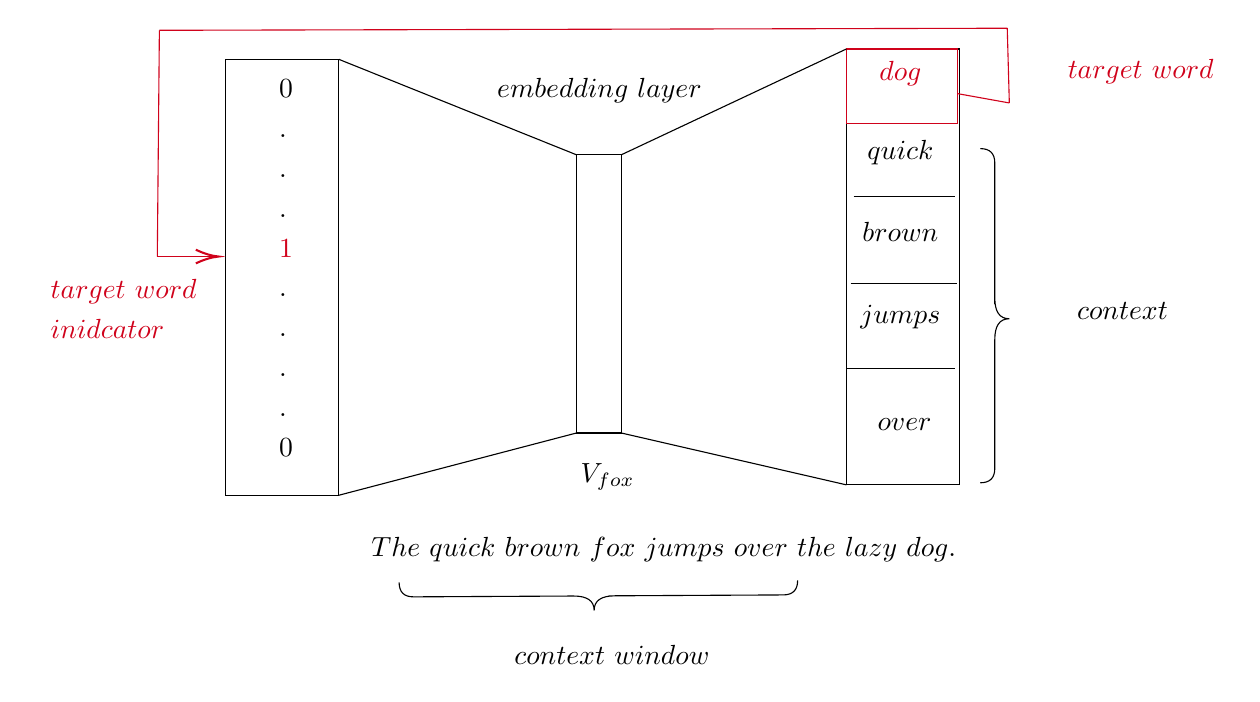
\begin{tikzpicture}[x=0.75pt,y=0.75pt,yscale=-1,xscale=1]
%uncomment if require: \path (0,347); %set diagram left start at 0, and has height of 347

%Shape: Rectangle [id:dp34856826620420023] 
\draw   (288,66) -- (309.5,66) -- (309.5,200) -- (288,200) -- cycle ;
%Shape: Rectangle [id:dp20385411601802828] 
\draw   (418,15) -- (472.5,15) -- (472.5,225) -- (418,225) -- cycle ;
%Shape: Rectangle [id:dp597929679831426] 
\draw  [color={rgb, 255:red, 208; green, 2; blue, 27 }  ,draw opacity=1 ] (418,15) -- (471.5,15) -- (471.5,51) -- (418,51) -- cycle ;
%Straight Lines [id:da329141353304766] 
\draw    (421.5,86) -- (470.5,86) ;


%Shape: Brace [id:dp7412735560954036] 
\draw   (202.5,272) .. controls (202.53,276.67) and (204.87,278.99) .. (209.54,278.96) -- (286.44,278.56) .. controls (293.11,278.53) and (296.45,280.84) .. (296.48,285.51) .. controls (296.45,280.84) and (299.77,278.49) .. (306.44,278.46)(303.44,278.47) -- (387.54,278.03) .. controls (392.21,278) and (394.53,275.66) .. (394.5,270.99) ;
%Straight Lines [id:da1987933863065281] 
\draw    (420,128) -- (471.5,128) ;


%Straight Lines [id:da8961013192322056] 
\draw    (418.5,169) -- (470.5,169) ;


%Shape: Brace [id:dp8413236825652046] 
\draw   (482.5,224) .. controls (487.17,224) and (489.5,221.67) .. (489.5,217) -- (489.5,154.97) .. controls (489.5,148.3) and (491.83,144.97) .. (496.5,144.97) .. controls (491.83,144.97) and (489.5,141.64) .. (489.5,134.97)(489.5,137.97) -- (489.5,70) .. controls (489.5,65.33) and (487.17,63) .. (482.5,63) ;
%Shape: Rectangle [id:dp5223635802427213] 
\draw   (119,20) -- (173.5,20) -- (173.5,230) -- (119,230) -- cycle ;
%Straight Lines [id:da26424324688833556] 
\draw [color={rgb, 255:red, 208; green, 2; blue, 27 }  ,draw opacity=1 ]   (86,115) -- (113.5,115) ;
\draw [shift={(115.5,115)}, rotate = 180] [color={rgb, 255:red, 208; green, 2; blue, 27 }  ,draw opacity=1 ][line width=0.75]    (10.93,-3.29) .. controls (6.95,-1.4) and (3.31,-0.3) .. (0,0) .. controls (3.31,0.3) and (6.95,1.4) .. (10.93,3.29)   ;

%Straight Lines [id:da3427921645180725] 
\draw [color={rgb, 255:red, 208; green, 2; blue, 27 }  ,draw opacity=1 ]   (87,6) -- (86,115) ;


%Straight Lines [id:da5378893688694539] 
\draw [color={rgb, 255:red, 208; green, 2; blue, 27 }  ,draw opacity=1 ]   (87,6) -- (495.5,5) ;


%Straight Lines [id:da1316572119067576] 
\draw [color={rgb, 255:red, 208; green, 2; blue, 27 }  ,draw opacity=1 ]   (495.5,5) -- (496.5,41) ;


%Straight Lines [id:da7079049036395544] 
\draw [color={rgb, 255:red, 208; green, 2; blue, 27 }  ,draw opacity=1 ]   (471.5,36.5) -- (496.5,41) ;


%Straight Lines [id:da6232994776605181] 
\draw    (173.5,20) -- (288,66) ;


%Straight Lines [id:da1671416061216935] 
\draw    (173.5,230) -- (288,200) ;


%Straight Lines [id:da8246799797542117] 
\draw    (309.5,66) -- (418,15) ;


%Straight Lines [id:da7881561473504775] 
\draw    (309.5,200) -- (418,225) ;



% Text Node
\draw (330,256) node   {$The\ quick\ brown\ fox\ jumps\ over\ the\ lazy\ dog.$};
% Text Node
\draw (303,221) node   {$V_{fox}$};
% Text Node
\draw (299,35) node   {$embedding\ layer$};
% Text Node
\draw (562,26) node [color={rgb, 255:red, 208; green, 2; blue, 27 }  ,opacity=1 ]  {$target\ word\ $};
% Text Node
\draw (444,27) node [color={rgb, 255:red, 208; green, 2; blue, 27 }  ,opacity=1 ]  {$dog$};
% Text Node
\draw (444,65) node   {$quick$};
% Text Node
\draw (444,103) node   {$brown$};
% Text Node
\draw (444,144) node   {$jumps$};
% Text Node
\draw (446,196) node   {$over$};
% Text Node
\draw (551,141) node   {$context$};
% Text Node
\draw (305,307) node   {$context\ window$};
% Text Node
\draw (148,121) node   {$ \begin{array}{l}
0\\
.\\
.\\
.\\
\textcolor[rgb]{0.82,0.01,0.11}{1}\\
.\\
.\\
.\\
.\\
0
\end{array}$};
% Text Node
\draw (72,141) node [color={rgb, 255:red, 208; green, 2; blue, 27 }  ,opacity=1 ]  {$ \begin{array}{l}
target\ word\ \\
inidcator
\end{array}$};


\end{tikzpicture}

}
\caption{Skip-gram architecture for the example sentence \emph{``The quick brown fox jumps over the lazy dog.''}. The input is the one-hot vector indicating the word \emph{``dog''} and the model tries to predict words that co-occur in the context window of the target word.  }
\label{fig:skip_w2v}
\end{figure}
\noindent
\textbf{The skip-gram} objective is to train word vector representations that are good at predicting the nearby words. A visual representation of the skip-gram model can be seen in Figure~\ref{fig:skip_w2v} for the sentence \emph{``The quick brown fox jumps over the lazy dog.''}, where the meaning of the word \emph{``fox''} is defined by the words in the window around it. The input is the one-hot vector for the the target word and the output is the context words.\\
More formally, given a corpus of words $f$ and their contexts $c$, to set the parameters $w$ of $p(c|f; w)$ so as to maximize the corpus probability, where $D$ is the set of all words and context pairs extracted from the text. Equation~\ref{eq:w2v_p} shows the probability formulation.
\begin{equation}
\label{eq:w2v_p}
w^*=\underset { w  }{ { \text{argmax} } } \prod _{ (w,c)\in D }^{  }{ p(c|f;  w )}
\end{equation}
The literature on neural-network language models, defines this probability using softmax shown in Equation~\ref{eq:w2v_softmax}, where $w_c$ and $ w_f\in R^d$ are vector representations for $c$ (context words) and $f$ (focal or center word) respectively, and
$C$ is the set of all available contexts. The goal is to find the parameters $w$ such that Equation~\ref{eq:w2v_p} is maximized~\brackettext{\cite{DBLP:journals/corr/GoldbergL14}}. 
\begin{equation}
\label{eq:w2v_softmax}
p(c|f;w)=\frac { { e }^{ w_{ c }.w_{ f } } }{ \sum _{ \acute { f } \in C }^{  }{ { e }^{ w_{ c }.w_{ \overline { f }  } } }  } 
\end{equation}
Maximizing the log-likelihood of Equation~\ref{eq:w2v_softmax} on the training set is very expensive. Because we need to compute and normalize each probability using the score for all other words  $\overline { f }$ in the context of $c$. Therefore, the authors reformulate the problem using \emph{Negative Sampling}~\brackettext{\cite{DBLP:journals/jmlr/GutmannH12}}. Negative sampling was used in order to deal with the expensive computation of the softmax, in which the multinomial classification problem (predicting the next word) is converted into a binary classification problem. To estimate a true probability distribution of the output word, binary logistic regression is used, where the classifier learns to distinguish between a true pair (true context words) and randomly selected words from the vocabulary (corrupted pairs). The classifier simply predicts whether a pair of words is a true or a random sample. to Equation~\ref{eq:w2v_negative}. $ \sigma$ shows the sigmoid function and $\overline{D}$ is the set of random $(f, c)$ pairs, assuming they are all incorrect. By maximizing this objective, the model assigns high probabilities to the real word pairs, and low probabilities to noise word pairs and it is more computationally appealing than the softmax function.

\begin{equation}
\label{eq:w2v_negative}
\underset { w }{ \mathrm{ argmax } } \quad \sum _{ (c,a)\in D }^{  }{ \log { \sigma ( } w_{ c }.w_{ a }) } +\sum _{ (c,f)\in \overline { D }  }^{  }{ \log { \sigma ( } -w_{ c }.w_{ f })\quad  } 
\end{equation}
If the model is trained on enough data, word2vec groups the vectors of similar words together in vector space, finds word’s associations and detects similarities mathematically with cosine similarity. 
%%%%%%%%%%%%%%%%%%%%%%%%%%%%%%%%%%%%%%%%%%%%%%%%%%%%%%%%%%%%
\subsection{GloVe: Global vector embeddings}
\label{subsec:GloVe}
The \emph{Global Vector Model} (GloVe) suggests that the ratio of co-occurrence probabilities can encode meaning components. An example can be seen in Table~\ref{table:tab_1}, in terms of studying a thermodynamic phase. A meaning component that sets the word \emph{``ice''} apart from \emph{``steam''} can be represented as a ratio of their occurrence probability with all other words \big($\frac { P(ice|k) }{ P(steam|k) } $, where $k$ can be any word in the vocabulary\big). This ratio is proven to better distinguish relevant words in comparison from irrelevant ones by giving the irrelevant ones a probability close to one. Also compared to the raw probabilities, it is better able to discriminate between the relevant words by giving a high probability to a word like \emph{``solid''} and low probability to \emph{``gas''}, making the word \emph{``ice''} stand out as a solid object. A word such as \emph{``water''} or \emph{``fashion''} will, therefore, have a probability close to one as it is either a shared property or not related to the concept.\\
\begin{table}[]
\centering

\begin{tabular}{@{}l|l|l|l|l@{}}
\toprule
Probability and Ratio &  $k=solid$& $k=gas$ & $k=water$ &$k= fashion$  \\ \midrule $P(k|ice)$& {\color[HTML]{CB0000}large} &  {\color[HTML]{329A9D}small} & {\color[HTML]{CB0000}large} & {\color[HTML]{329A9D}small} \\\midrule
  $P(k|steam)$&{\color[HTML]{329A9D}small}  & {\color[HTML]{CB0000}large} &  {\color[HTML]{CB0000}large}&{\color[HTML]{329A9D}small}  \\\midrule
 $\frac { P(ice|k) }{ P(steam|k) } $& {\color[HTML]{CB0000}large} &  {\color[HTML]{329A9D}small}&  1 &    1  \\\midrule
\end{tabular}%
\caption{Co-occurrence probabilities for target words \emph{``ice''}and \emph{``steam''} with selected context words. Example taken from~\brackettext{\cite{DBLP:conf/emnlp/PenningtonSM14}}.}
\label{table:tab_1}
\end{table}
\noindent
To capture these ratios, the authors of GloVe propose a log-bilinear model, where, if the dot product of two vectors corresponds to the log of their co-occurrence probability, their difference will show the meaning component, as seen in Equation~\ref{eq:log_prob}. Let the matrix of word-word co-occurrence counts be denoted by $X\in { R }^{ |V|\times |V| }$, where $|V|$ is the size of the vocabulary. Entries $X_{ij}$ tabulate the number of times word $j$ occurs in the context of word $i$. $w_{ i }\in { R }^{ 1\times M }$ and $\tilde{w_{ j }}\in { R }^{ 1\times M }$ are the focal (center word) and context embeddings, respectively, where $M$ is the embedding size. The model tries to learn embeddings that minimize the squared difference between the dot product of the center word embedding and context embedding to the logarithm of its co-occurrence.
\begin{equation}
\begin{split}
\\ w_{ i }.w_{ j }=\log { P(i|j)\quad  } \\
w_{ x }(w_{ i }-w_{ j })=\log { \frac { P(x|j) }{ P(x|j) } } 
\end{split}
\label{eq:log_prob}
\end{equation}
Considering $ \tilde{b_{ j }}$ and $b_{ i }$  as the biases for the focal and context embeddings, the cost function is defined in Equation~\ref{eq:glove_cost}. Since the log of co-occurrences does not directly result in a probability, in order for the meaning component to have a probabilistic interpretation, a normalization factor is needed. Bias $b_{ i }$ allows the model to learn this constant during training and $ \tilde{b_{ j }}$ is added to preserve symmetry. 
\begin{equation}
J=\sum _{ i,j=1 }^{ |V| }{ f({ X }_{ ij } } )(w_{ i }^{ \top }\tilde{  w_{ j } } +b_{ i }+\tilde{  b_{ j } } -\log{ X }_{ ij })^2
\label{eq:glove_cost}
\end{equation}
Optimizing for the co-occurrence counts alone might cause the model to overemphasize the most common words. Therefore, a weighing function $f$ is introduced that imposes an upper bound on the maximum number of occurrences of a word. Conceptually, $f$ scales the counts in order to avoid the influence of common words and boost the rare words. The choice of $f$ is not fixed but one class of functions that were used by the authors can be parametrized with $\alpha$ as the exponential weight and $x_{max}$ as the maximum number of allowed co-occurrences. $\alpha$ and $x_{max}$ are hyper-parameters that require tuning, but the values suggested by the authors are $\frac{3}{4}$ for $\alpha$ is  and $100$ for $x_{max}$. 
\begin{equation}
f=\left\{
  \begin{array}{@{}ll@{}}
    (\frac { x }{ { x }_{ \max } } )^{ \alpha  }& \text{if}\ x<x_{max} \\
    1 & \text{otherwise}
  \end{array}\right.
\label{eq:weighingfunction}
\end{equation}
\noindent
The model learns two embeddings for each word, one as a focal or center word and the other as a context word. As the co-occurrence matrix is symmetric both of which can be considered as learning the same representation. Ultimately, the two embeddings can be added to obtain the final embedding.
%%%%%%%%%%%%%%%%%%%%%%%%%%%%%%%%%%%%%%%%%%%%%%%%%%%%%%%%%%%%
\subsection{Similarity between embeddings}\label{sec:similarity}
The dense word vector is learned to capture the semantics of the words and hence similar words are close in the induced space. \emph{Cosine similarity} helps to capture this semantic closeness and is the most common similarity measure for the word vector. The cosine similarity is a measure that calculates the cosine of the angle between two vectors. This metric is a measurement of orientation and not magnitude and it is derived from the equation of a dot product between two vectors (Equation~\ref{eq:cosine}). The vectors are normalized by their length, which removes the influence of their magnitude on the similarity. The norm of the vector is somewhat related to the overall frequency of which words occur in the training corpus, but the direction is unaffected by this. So in order for a common word like \emph{``frog''} to still be similar to a less frequent word like \emph{``Anura''} (a type of frog), cosine distance which only looks at the direction works better than simple Euclidean distance. Moreover, cosine similarity is symmetric and therefore, changing the order of vectors in the dot product does not affect the final result.
\begin{equation}
\begin{split}
\overrightarrow { w_i } .\overrightarrow { w_j } =\parallel \overrightarrow { w_i } \parallel \parallel \overrightarrow { w_j } \parallel cos\theta 
\\
cos\theta =\frac { \overrightarrow { w_i } .\overrightarrow { w_j }  }{ \parallel \overrightarrow { w_i } \parallel \parallel \overrightarrow { w_j } \parallel  } 
\end{split}
\label{eq:cosine}
\end{equation}
%%%%%%%%%%%%%%%%%%%%%%%%%%%%%%%%%%%%%%%%%%%%%%%%%%%%%%%%%%%%
\subsection{Edge weights and co-occurrence probabilities}\label{subsec:weights_load}
The cost function of the GloVe model is based on the assumption that the ratio of co-occurrence probabilities result in meaningful components, which can be investigated to find the relation between two words. Edge weights of the LOAD model have a correlation with the co-occurrence counts of terms and entities in text. However, the sentence distance is a more efficient way to define a distance metric between two entities rather than a window-based approach. As two entities appearing in the same document tend to have some connection, this relationship is disregarded if we only look at a small window of words. Additionally, since the weights decay based on how far an entity is from another gives us more information about the structure of the text. Based on these considerations, we argue that LOAD edge weights produce a better overall corpus statistics in case of named entities with respect to a simple co-occurrence matrix and that it can generate the same meaningful components like probability ratios. \\
We demonstrate this with a simple example in Table~\ref{table:tab_2} that shows how certain aspects of meaning can be extracted from edge weights of LOAD. Suppose we are interested in the concept of US presidents, for which we take two actors \emph{``Donald Trump''} and \emph{``Barack Obama''}. The relationship between these entities can be examined by studying the ratio of their edge weights with various probe words. Similar to the GloVe model, where the ratio of co-occurrence probability distinguished the relevant words from irrelevant words, here the ratio of the edge weights works in the same way. In this case, looking at the raw edge weights does not give us much comparable information, but the ratio denotes \emph{``Donald Trump''} as a republican rather than a democratic politician. Since both of the entities share the presidential attribute the ratio is close to one. On the other hand, a random name like \emph{``BMW''} has a relatively small weight with both entities, but since the weak edges were cut off from the model we have the weight of zero. Considering the full graph without a cut-off threshold, the ratio of two small numbers will also converge to one, implying that same as co-occurrence matrix, edge weights of LOAD contain these meaning components. Consequently, the bilinearity assumption of GloVe can be extended to the weighted adjacency matrix of LOAD. 
\begin{table}[]
\centering

\begin{tabular}{@{}l|l|l|l|l@{}}
\toprule
Probability and Ratio&  $k=republican$& $k=democratic$ & $k=president$ &$k= BMW$  \\ \midrule
 $P(k|Trump)$& {\color[HTML]{CB0000}10.51} &  {\color[HTML]{329A9D}5.30} & {\color[HTML]{CB0000}52} & {\color[HTML]{329A9D}0} \\\midrule
  $P(k|Obama)$&{\color[HTML]{329A9D}0.36}  & {\color[HTML]{CB0000}1.29} &  {\color[HTML]{CB0000}66}&{\color[HTML]{329A9D}0}  \\\midrule
 $\frac { P(Trump|k) }{ P(Obama|k) } $& {\color[HTML]{CB0000}29.2} &  {\color[HTML]{329A9D}4.10}&  0.78 &    0  \\\midrule
\end{tabular}%

\caption{LOAD weights for target words \emph{``Donald Trump''} and \emph{``Barack Obama''} with selected context words. }
\label{table:tab_2}
\end{table}
\label{sec:components_load}

%%%%%%%%%%%%%%%%%%%%%%%%%%%%%%%%%%%%%%%%%%%%%%%%%%%%%%%%%%%%
\section{Entity Embeddings}
\label{sec:enity_embed}
Entity embedding are mostly studied in the concept of embedding knowledge graphs as part of a downstream task, mostly for entity disambiguation. Guo and Barbosa use random walks on knowledge graphs to construct vector representations of entities for named entity disambiguation task~\brackettext{\cite{DBLP:journals/semweb/GuoB18}}. He et al. use a deep neural network to represent the entities and their relations in knowledge graphs for inference tasks and link prediction~\brackettext{\cite{DBLP:journals/corr/YangYHGD14a}}. Other than pure knowledge graph embedding, a few models focus on combining the word embeddings with embeddings from knowledge graphs for enity disambiguation tasks. In a paper by Yamada et al., the skip-gram model is combined with knowledge graph embeddings, where the vectors are aligned, such that similar words and entities occur close to one another in the vector space. The learned embeddings are then used as a feature for named entity disambiguation~\brackettext{\cite{DBLP:conf/conll/YamadaS0T16}}. Fang et al. also take a similar approach and learn word embeddings from text and entity embeddings from a knowledge graph. They later use an alignment model that guarantees the vectors of entities and words are in the same space and utilize them to design feature for their disambiguation framework~\brackettext{\cite{DBLP:conf/conll/FangZWCL16}}. These methods, although successful at representing entity and words are dependent on the knowledge bases as an extra source of information. They often optimize different objective functions for learning the entity embeddings and word embeddings, or train them separately and combine them in a later step. In this thesis, we avoid using separate training objectives for entities and word and treat them equally to learn embeddings directly from annotated text. It is also important to note that since these embedding are designed as feature for a specific task, they are only evaluated through the performance of that task. In contrast, we focus on creating general purpose entity embeddings that are comparable to normal word embeddings and evaluate them against the state-of-the-art word embedding techniques to asses their difference in performance. \\

%%%%%%%%%%%%%%%%%%%%%%%%%%%%%%%%%%%%%%%%%%%%%%%%%%%%%%%%%%%%
\section{Graph-based Embeddings}
\label{sec:graph}
Graph embeddings convert a graph into a low dimensional space in which the graph information is preserved. Therefore, it is an effective and efficient way to compute features from a graph for machine learning algorithms. Based on the embedding output, graph embeddings are categorized into four types: \emph{node embedding}, \emph{edge embedding}, \emph{hybrid embedding} (combination of different types of graph components, e.g., node $+$ edge), and  \emph{whole-graph embedding} (a graph is represented as one vector)~\brackettext{\cite{DBLP:journals/tkde/CaiZC18}}. Different node embedding models vary in their definition of similarity between nodes and the graph property they preserve. Two of the most important properties are \emph{first-order proximity} and \emph{second-order proximity}. First-order proximity captures the direct neighbourhood relationship (edges) in a graph. Second-order proximity captures the $2$-end step relations (number of common neighbors shared). The second-order proximity can also be extended to take higher orders into account as well~\brackettext{\cite{DBLP:journals/jmlr/GutmannH12}}.\\
Since the nodes of the co-occurrence graph correspond to words in the vocabulary, in this study we only look at node embedding techniques. Embedding the edges or whole graph does not provide any information about the words of the corpus. In the following we give a brief introduction into popular node embedding methods. 
%%%%%%%%%%%%%%%%%%%%%%%%%%%%%%%%%%%%%%%%%%%%%%%%%%%%%%%%%%%%
\subsection{DeepWalk, a random walk-based embedding}
\label{subsec:DeepWalk}
\begin{figure}
\centering 
\resizebox{0.8\textwidth}{0.35\textwidth}{      
\input{images/DeepWalk.tex}
}
\caption{The workflow of DeepWalk. It first generates random walk sequences from a graph, and then applies the skip-gram model to learn the embeddings. Figure adapted from~\brackettext{\cite{SCHOL:journal/IEEE/zahng}}.}
\label{fig:deepwalk}
\end{figure}

The \emph{DeepWalk}~\brackettext{\cite{DBLP:conf/kdd/PerozziAS14}} model learns latent representations of nodes of a graph using local information obtained from fixed length random walks. The model treats the nodes visited in the random walk as words and the walk itself as  a sentence from the corpus. Then the skip-gram is applied on the generated corpus to maximize the probability of visiting the neighbourhood of the node conditioned on its embedding. A visualization of the workflow of DeepWalk is shown in Figure~\ref{fig:deepwalk}. In other words, the model tries to learn the embedding $w\in R^{ d} $, where $d$ is a small number of latent dimensions in comparison to the number of nodes. The model maximizes the probability of observing the last $k$ nodes and the next $k$ nodes in the random walk entered at node $v_{i}$, by minimizing negative log of the probability as shown in the Equation~\ref{eq:dw}, to learn the node embedding $w$~\brackettext{\cite{DBLP:journals/kbs/GoyalF18}}.: 
\begin{equation}
J=-\log { P( } v_{ { i−k } },...,v_{ i−1 },v_{ i+1 },...,v_{ i+k }|w )
\label{eq:dw}
\end{equation}
Based on this approach, nodes that share similar neighbours in random walk sequences should be represented closely in the embedding space. Since the random walk in DeepWalk correspond to the \emph{Depth-first Sampling}(DFS) , it can preserve the second-order proximity. As a result, DeepWalk is good at keeping community structures. 
%%%%%%%%%%%%%%%%%%%%%%%%%%%%%%%%%%%%%%%%%%%%%%%%%%%%%%%%%%%%
\subsection{Node2vec: Scalable feature learning for graphs }
\label{subsec:node2vec}
\emph{Node2vec}~\brackettext{\cite{DBLP:conf/kdd/GroverL16}} extends the random walk procedure of DeepWalk by defining a more flexible notion of a node’s neighborhood. There are mainly two node sampling strategies in random walk: \emph{Breadth-first Sampling} (BFS) and \emph{Depth-first Sampling} (DFS), where the BFS focuses on the immediate neighbors of the node and DFS consists of sampled nodes sequentially sampled at increasing distances from the source node~\brackettext{\cite{DBLP:conf/kdd/GroverL16}}.
Therefore, BFS represents the first-order proximity and DFS the second and higher-order proximity. A demonstration of different sampling methods is provided in Figure~\ref{fig:dfs_bfs}. Node2vec provides a trade-off between BFS and DFS. Node2vec uses two hyperparameters to regulate the balance between the two methods. By choosing a right balance between the two sampling methods, we preserve community structure as well as structural equivalence between nodes~\brackettext{\cite{DBLP:journals/kbs/GoyalF18}}.
However, the node2vec method tends to be quite inefficient for large graphs and incurs significant space and time overhead. It runs out of memory even for mid-sized graphs. Although there exist complex graph structures to speed up the process, the original model is very slow on large graphs ~\brackettext{\cite{DBLP:journals/corr/abs-1805-00280}}. 
\begin{figure}
\centering 
\resizebox{0.45\textwidth}{0.25\textwidth}{      
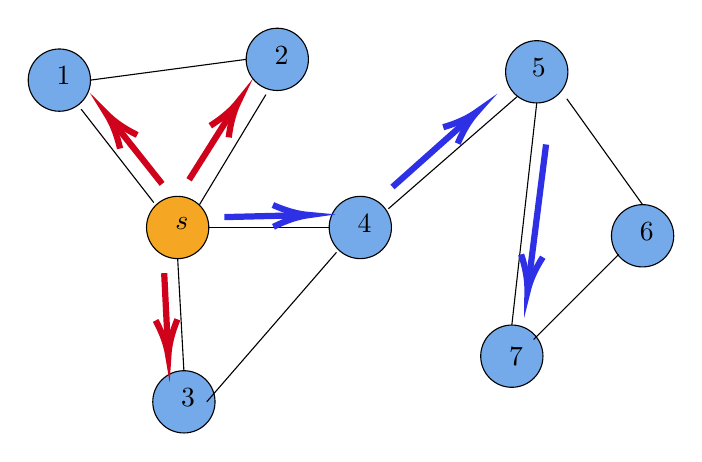
\begin{tikzpicture}[x=0.75pt,y=0.75pt,yscale=-1,xscale=1]
%uncomment if require: \path (0,407); %set diagram left start at 0, and has height of 407

%Shape: Circle [id:dp332493301566809] 
\draw  [fill={rgb, 255:red, 74; green, 144; blue, 226 }  ,fill opacity=0.77 ] (56,81) .. controls (56,72.72) and (62.72,66) .. (71,66) .. controls (79.28,66) and (86,72.72) .. (86,81) .. controls (86,89.28) and (79.28,96) .. (71,96) .. controls (62.72,96) and (56,89.28) .. (56,81) -- cycle ;
%Shape: Circle [id:dp4879070023914207] 
\draw  [fill={rgb, 255:red, 245; green, 166; blue, 35 }  ,fill opacity=1 ] (113,152) .. controls (113,143.72) and (119.72,137) .. (128,137) .. controls (136.28,137) and (143,143.72) .. (143,152) .. controls (143,160.28) and (136.28,167) .. (128,167) .. controls (119.72,167) and (113,160.28) .. (113,152) -- cycle ;
%Shape: Circle [id:dp5810034132491635] 
\draw  [fill={rgb, 255:red, 74; green, 144; blue, 226 }  ,fill opacity=0.77 ] (161,71) .. controls (161,62.72) and (167.72,56) .. (176,56) .. controls (184.28,56) and (191,62.72) .. (191,71) .. controls (191,79.28) and (184.28,86) .. (176,86) .. controls (167.72,86) and (161,79.28) .. (161,71) -- cycle ;
%Shape: Circle [id:dp678091001536465] 
\draw  [fill={rgb, 255:red, 74; green, 144; blue, 226 }  ,fill opacity=0.77 ] (116,236) .. controls (116,227.72) and (122.72,221) .. (131,221) .. controls (139.28,221) and (146,227.72) .. (146,236) .. controls (146,244.28) and (139.28,251) .. (131,251) .. controls (122.72,251) and (116,244.28) .. (116,236) -- cycle ;
%Shape: Circle [id:dp19856877490785307] 
\draw  [fill={rgb, 255:red, 74; green, 144; blue, 226 }  ,fill opacity=0.77 ] (201,152) .. controls (201,143.72) and (207.72,137) .. (216,137) .. controls (224.28,137) and (231,143.72) .. (231,152) .. controls (231,160.28) and (224.28,167) .. (216,167) .. controls (207.72,167) and (201,160.28) .. (201,152) -- cycle ;
%Shape: Circle [id:dp06052439820005162] 
\draw  [fill={rgb, 255:red, 74; green, 144; blue, 226 }  ,fill opacity=0.77 ] (286,77) .. controls (286,68.72) and (292.72,62) .. (301,62) .. controls (309.28,62) and (316,68.72) .. (316,77) .. controls (316,85.28) and (309.28,92) .. (301,92) .. controls (292.72,92) and (286,85.28) .. (286,77) -- cycle ;
%Shape: Circle [id:dp7842135850860721] 
\draw  [fill={rgb, 255:red, 74; green, 144; blue, 226 }  ,fill opacity=0.77 ] (274,214) .. controls (274,205.72) and (280.72,199) .. (289,199) .. controls (297.28,199) and (304,205.72) .. (304,214) .. controls (304,222.28) and (297.28,229) .. (289,229) .. controls (280.72,229) and (274,222.28) .. (274,214) -- cycle ;
%Shape: Circle [id:dp69600261549569] 
\draw  [fill={rgb, 255:red, 74; green, 144; blue, 226 }  ,fill opacity=0.77 ] (337,156) .. controls (337,147.72) and (343.72,141) .. (352,141) .. controls (360.28,141) and (367,147.72) .. (367,156) .. controls (367,164.28) and (360.28,171) .. (352,171) .. controls (343.72,171) and (337,164.28) .. (337,156) -- cycle ;
%Straight Lines [id:da49057224619926565] 
\draw    (81.5,95) -- (116.5,140) ;


%Straight Lines [id:da40111900668895095] 
\draw    (128,167) -- (131,221) ;


%Straight Lines [id:da3149529915409619] 
\draw    (170.5,88) -- (138.5,141) ;


%Straight Lines [id:da40356254390150004] 
\draw    (143,152) -- (201,152) ;


%Straight Lines [id:da11721701648427074] 
\draw    (142,236) -- (204.5,164) ;


%Straight Lines [id:da7531222279660781] 
\draw    (86,81) -- (161,71) ;


%Straight Lines [id:da6126183155613649] 
\draw    (291.5,89) -- (229.5,143) ;


%Straight Lines [id:da4426831658921855] 
\draw    (315.5,90) -- (352,141) ;


%Straight Lines [id:da44944128673840367] 
\draw    (301,92) -- (289,199) ;


%Straight Lines [id:da49417599304234616] 
\draw    (340.5,165) -- (299.5,206) ;


%Straight Lines [id:da9093872174761735] 
\draw [color={rgb, 255:red, 208; green, 2; blue, 27 }  ,draw opacity=1 ][line width=2.25]    (120.5,131) -- (95.99,100.13) ;
\draw [shift={(93.5,97)}, rotate = 411.55] [color={rgb, 255:red, 208; green, 2; blue, 27 }  ,draw opacity=1 ][line width=2.25]    (17.49,-5.26) .. controls (11.12,-2.23) and (5.29,-0.48) .. (0,0) .. controls (5.29,0.48) and (11.12,2.23) .. (17.49,5.26)   ;

%Straight Lines [id:da13977987756203492] 
\draw [color={rgb, 255:red, 208; green, 2; blue, 27 }  ,draw opacity=1 ][line width=2.25]    (133.5,129) -- (155.36,94.38) ;
\draw [shift={(157.5,91)}, rotate = 482.28] [color={rgb, 255:red, 208; green, 2; blue, 27 }  ,draw opacity=1 ][line width=2.25]    (17.49,-5.26) .. controls (11.12,-2.23) and (5.29,-0.48) .. (0,0) .. controls (5.29,0.48) and (11.12,2.23) .. (17.49,5.26)   ;

%Straight Lines [id:da447165384934876] 
\draw [color={rgb, 255:red, 208; green, 2; blue, 27 }  ,draw opacity=1 ][line width=2.25]    (121.5,174) -- (123.3,210) ;
\draw [shift={(123.5,214)}, rotate = 267.14] [color={rgb, 255:red, 208; green, 2; blue, 27 }  ,draw opacity=1 ][line width=2.25]    (17.49,-5.26) .. controls (11.12,-2.23) and (5.29,-0.48) .. (0,0) .. controls (5.29,0.48) and (11.12,2.23) .. (17.49,5.26)   ;

%Straight Lines [id:da7666273172002611] 
\draw [color={rgb, 255:red, 46; green, 48; blue, 230 }  ,draw opacity=1 ][line width=2.25]    (150.5,147) -- (187.5,146.1) ;
\draw [shift={(191.5,146)}, rotate = 538.6] [color={rgb, 255:red, 46; green, 48; blue, 230 }  ,draw opacity=1 ][line width=2.25]    (17.49,-5.26) .. controls (11.12,-2.23) and (5.29,-0.48) .. (0,0) .. controls (5.29,0.48) and (11.12,2.23) .. (17.49,5.26)   ;

%Straight Lines [id:da7337308124937729] 
\draw [color={rgb, 255:red, 46; green, 48; blue, 230 }  ,draw opacity=1 ][line width=2.25]    (231.5,132.5) -- (269.51,98.66) ;
\draw [shift={(272.5,96)}, rotate = 498.32] [color={rgb, 255:red, 46; green, 48; blue, 230 }  ,draw opacity=1 ][line width=2.25]    (17.49,-5.26) .. controls (11.12,-2.23) and (5.29,-0.48) .. (0,0) .. controls (5.29,0.48) and (11.12,2.23) .. (17.49,5.26)   ;

%Straight Lines [id:da34116815343810125] 
\draw [color={rgb, 255:red, 46; green, 48; blue, 230 }  ,draw opacity=1 ][line width=2.25]    (305.5,112) -- (297,179.03) ;
\draw [shift={(296.5,183)}, rotate = 277.22] [color={rgb, 255:red, 46; green, 48; blue, 230 }  ,draw opacity=1 ][line width=2.25]    (17.49,-5.26) .. controls (11.12,-2.23) and (5.29,-0.48) .. (0,0) .. controls (5.29,0.48) and (11.12,2.23) .. (17.49,5.26)   ;


% Text Node
\draw (73,79) node   {$1$};
% Text Node
\draw (130,150) node   {$s$};
% Text Node
\draw (178,69) node   {$2$};
% Text Node
\draw (133,234) node   {$3$};
% Text Node
\draw (218,150) node   {$4$};
% Text Node
\draw (302,75) node   {$5$};
% Text Node
\draw (291,214) node   {$7$};
% Text Node
\draw (354,154) node   {$6$};


\end{tikzpicture}

}
\caption{DFS and BFS sampling for a random walk with length $3$ from the start node \emph{``s''}. The figure is adapted from ~\brackettext{\cite{DBLP:conf/kdd/GroverL16} }.}
\label{fig:dfs_bfs}
\end{figure}
%%%%%%%%%%%%%%%%%%%%%%%%%%%%%%%%%%%%%%%%%%%%%%%%%%%%%%%%%%%%
\subsection{LINE: Large-scale information network embedding}
\label{subsec:LINE}
The \emph{Large-scale Information Network Embedding} (LINE) model~\brackettext{\cite{DBLP:conf/www/TangQWZYM15}} does not use random walks, instead it optimizes two objective functions, one each for first- and second-order proximities, and minimizes the combination of the two to achieve two embeddings. The first objective function aims to keep the adjacency matrix and dot product of embeddings close. The LINE model defines two joint probability distributions for each pair of nodes, one using an adjacency matrix and the other using the embedding and minimizes the KL-divergence between the distributions. The first objective results into the first half of the embedding. The authors define probability distributions and objective function for the second half based on the the second-order proximity~\brackettext{\cite{DBLP:journals/kbs/GoyalF18}}. Nevertheless, the model fails to learn meaningful representation of graphs with unbalanced edge weights. The objective function for the second-order proximity is ill-defined when the weight of edges have a high variance~\brackettext{\cite{DBLP:conf/www/TangQWZYM15}}.
%%%%%%%%%%%%%%%%%%%%%%%%%%%%%%%%%%%%%%%%%%%%%%%%%%%%%%%%%%%%
\subsection{VERSE: Versatile graph embeddings from similarity measures}
\label{subsec:VERSE}
The \emph{Versatile Graph Embeddings from Similarity Measures} (VERSE)~\brackettext{\cite{DBLP:conf/www/TsitsulinMKM18}} model learns embeddings by training a single-layer neural network, which can be instantiated with diverse similarity measures. Given a graph $G=(V,E)$, where $V$ is the set of nodes and $E$ the set of all edges, the aim is to learn the node embedding $w \in R^{d}$, where $d$ is a small number of latent dimensions, by optimizing the objective function in Equation~\ref{eq:VERSE}. In optimization objective, the KL-divergence from the given similarity distribution $sim_G$ to that of $sim_E$ in the embedded space is minimized, for any node $v$. 
\begin{equation}
\sum _{ v\in V }^{  }{ KL(sim_{ G }(v,.),sim_{ E } } (v,.))
\label{eq:VERSE}
\end{equation}
The similarity of two nodes in the embedding space is related to their dot product in the embedding space. Therefore, the similarity distribution ( $sim_E$) between two nodes $i$ and $j$ in the embedded space is their dot product ($w_i . w_j$), normalized with softmax, as shown in Equation~\ref{eq:VERSE_simE}. We should minimize the KL-divergence between the $sim_{ E }$ and an arbitrary similarity measure for the nodes to produce node embeddings. 
\begin{equation}
sim_{ E }(v,.)=\frac{ w_{ v }.W^\top }{ \sum _{ i=1 }^{ n }{ \exp{(w_{ v }.w_{ i }) }}  }\label{eq:VERSE_simE}
\end{equation}
Although VERSE is designed to accept any similarity measure, three measures are contained in the original implementation: \emph{Personalized PageRank} (PPR),  \emph{Adjacency Similarity}, and  \emph{SimRank}. PPR is based on the stationary distribution of a random walk with restart. Thus, this measure is closely related to DeepWalk and node2vec. SimRank is a measure of structural relatedness. If two nodes are connected to similar nodes they are themselves considered similar. Adjacency Similarity is based on the normalized adjacency matrix. More formally, given the out degree $Out(v_{i})$ of node $v_{i}$, $sim_{ G }$ for the Adjacency Similarity is shown in Equation~\ref{eq:VERSE_simG}~\brackettext{\cite{DBLP:conf/www/TsitsulinMKM18}}. 
\begin{equation}
sim^{ ADJ }_{ G }(v_{ i },v_{ j })=\left\{ \begin{matrix} \frac { 1 }{ Out(v_{ i }) } \quad if\quad (v_{ i },v_{ j })\in E\quad  \\ 0\quad \qquad \qquad \mathrm{otherwise} \end{matrix} \right.\label{eq:VERSE_simG}
\end{equation}
Since the optimization objective is expensive, the \emph{VERSE} samples positive and negative samples with \emph{Noise Contrastive Estimation} (NCE)~\brackettext{\cite{DBLP:journals/jmlr/GutmannH12}} to converge to a solution. NCE is same as Negative Sampling used in word2vec. The difference is that in word2vec words for the negative samples are drawn from a specially designed distribution, which favours less frequent words. \\


In Chapters~\ref{chap:entity} and \ref{chap:faceted}, we use the background information presented in this chapter about the word embedding and graph embedding techniques to define our entity embedding and faceted embedding models from entity annotated text.

   \chapter{Entity Embeddings}\label{chap:entity}

In this chapter, we try to explore different ways to train word embeddings for entities and terms jointly. We use the word embedding and graph embedding models explained in the previous chapter, on annotated data to generate such embeddings. In Section~\ref{sec:entity_overview}, an overview of all models is given and the objectives are explained. Section~\ref{sec:raw} is dedicated to models trained on unannotated (raw) text, that are used as the baseline against which we compare our models. The remaining two sections describe the two entity-based models proposed in this thesis. In Section~\ref{sec:annotated},  word embeddings that are trained on annotated text are explained, followed by graph-based models in Section~\ref{sec:graph_based}. Finally, we explain how to measure the similarity between two embeddings in Section~\ref{sec:similarity}
\ornament
We introduce entity-based embeddings to address the issues that entity-centric downstream tasks would face when using word embeddings as features. An annotated corpus has many benefits. To name a few: 
\emph{Distinguishing homographs:} with annotation, we can distinguish between entity homographs. As a result, a vector representation of \emph{``Washington''} as a person is different from the same word as location. \\
\emph{Embedding compound words:}  unlike raw text, where the compound name is broken down into specific parts, names of entities are grouped into a unique identifier that helps the model to learn a distinct representation for it.  In traditional methods, to derive a unique representation for an entity like \emph{``Donald Trump"}, embeddings for two parts of the word have to be averaged, multiplied or transformed in some post-processing step, which is not only inefficient but also misleading; as the name \emph{``Donald"} can refer to many other \emph{``Donalds"} in a different contexts. \\
\emph{Unifying all surface form of an entity:} Mentions of the same entity with different surface forms are considered a unit identity, e.g., \emph{``Obama''} and \emph{``Mr. President''} in the time frame after $2009$, which creates a word context pair for each entity, which can increase performance. For example, all the words surrounding \emph{``Obama''} or any of aliases are considered as context word for the entity \emph{``Barack Obama''}. \\
We identify expressions which are dates or time, and normalise them into a single unique date. Hence, we can incorporate the temporal information as the context of a word, and at the same time learn a vector representation for the dates. \\
\emph{Customizable search:} Since entities have pre-defined types, such as actor or location, we can perform a more effective search in the embedding space. The neighbourhood of a word can be filtered to contain only relevant types, which is beneficial for finding relationships between people or organizations. \\
\emph{Flexible neighbourhood definition:} In a term-based model, a word is only defined by the terms surrounding it. With annotated named entities now we can have different definitions of a word, based on the type of entities surrounding it. A word can be defined by the most relevant locations or actors. For example, when looking for the nearest neighbour of a word, the neighbourhood can be filtered to contain only entities of a specific type or remove the entities altogether and look only at surrounding terms. We take advantage of this property in Chapter~\ref{chap:eval} and introduce a new search criterion that succeeds in capturing entity-entity relations better than term-based models. \\

In general, removing ambiguous mentions and annotating the corpus provides the models with more information and is stand to produce better input features for entity related tasks, such as information retrieval~\brackettext{\cite{DBLP:conf/acl/0001MC16,DBLP:conf/cikm/KuziSK16}}, named entity recognition~\brackettext{\cite{DBLP:conf/nodalida/Siencnik15}}. Since the concept of embedding named entities has not been studied until now, there is no framework available that uses such embeddings as an input. Consequently, the claim for better performance in any downstream task can only be validated if such frameworks are created. As a result, in this thesis, we only focus on creating entity embeddings that can perform similar or better to normal word embeddings on the common term-based evaluation tasks.
\section{Overview and Objectives}\label{sec:entity_overview}
In this chapter, we introduce methods for training entity and term embeddings jointly, on an annotated corpus.The main objective of entity-based models is to upgrade the traditional term embeddings, by incorporating the type of the word and also to learn a unique representation for named entities mentioned in the text. We focus on learning these embeddings by tweaking the existing word and graph embedding techniques and evaluating which one works best. For this purpose, propose two approaches: 
\begin{compactenum}
\item To naively include entities in the embeddings, we train the well-established word embedding models on a corpus, annotated with named entities. 
\item Embedding the nodes of co-occurrence graphs extracted from the annotated text. 
\end{compactenum}
Both of the models are compared against word embedding models trained on raw text. To achieve better performance, we try a wide range of different techniques, starting from the well-established word embeddings methods on annotated corpus to graph embedding techniques on word co-occurrence graphs. As described later in the Chapter~\ref{chap:eval}, the first method produces poor results on our evaluation tasks. Hence, the graph-based models are proposed to solve this problem. 
\section{Word Embeddings on Raw Text}\label{sec:raw}
State-of-the-art word embedding models are trained on raw text (without entity annotation). The word2vec and GloVe models, explained in Chapter~\ref{chap:background}, Sections~\ref{subsec:word2vec} and~\ref{subsec:GloVe} respectively, are chosen as representative of classical word embeddings. From the word2vec model, the skip-gram architecture is chosen. We refer to the word2vec and GloVe model as $r$W2V and  $r$GLV, where \emph{``r"} denotes raw text input. The text is cleaned only by common pre-processing steps.  Since no entities are annotated, all words are treated as terms. 
\section{Word Embeddings on Annotated Text}\label{sec:annotated}
\begin{figure}
\centering 
\resizebox{0.85\textwidth}{0.28\textwidth}{      
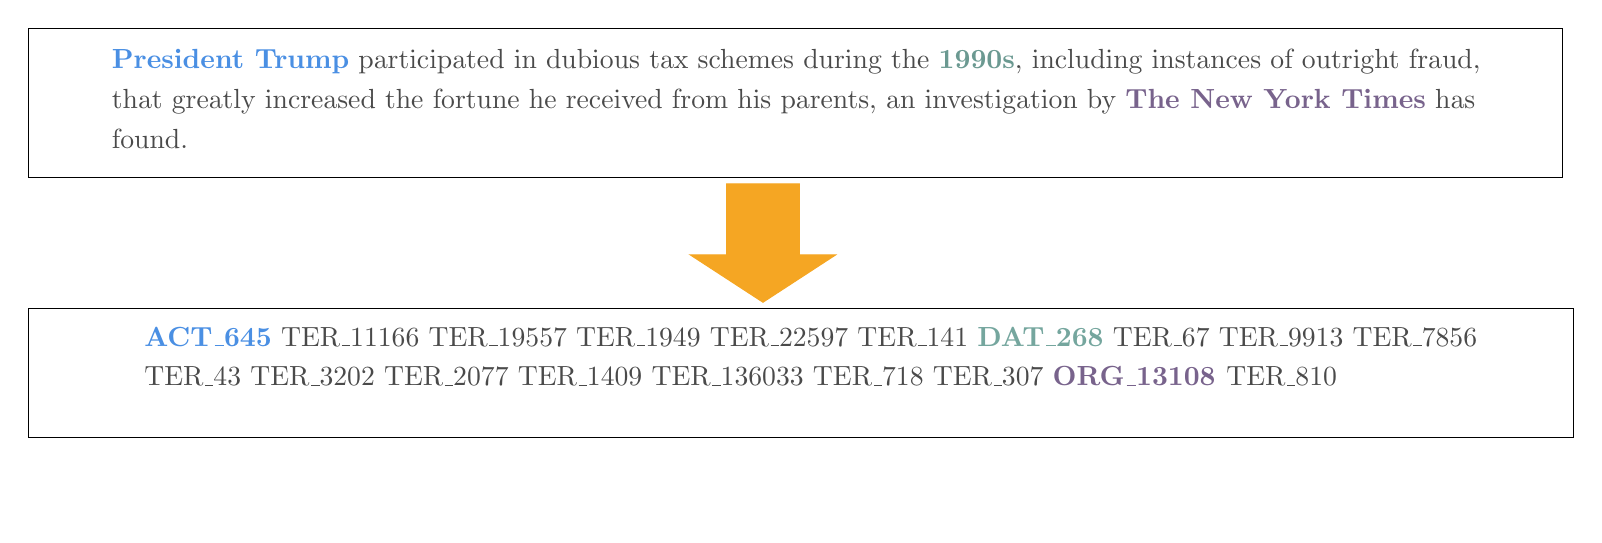
\begin{tikzpicture}[x=0.75pt,y=0.75pt,yscale=-1,xscale=1]
%uncomment if require: \path (0,377); %set diagram left start at 0, and has height of 377

%Shape: Rectangle [id:dp8906489990544584] 
\draw   (28,17) -- (767,17) -- (767,89) -- (28,89) -- cycle ;
%Shape: Rectangle [id:dp9074920271044917] 
\draw   (28,152) -- (772.5,152) -- (772.5,214) -- (28,214) -- cycle ;
%Down Arrow [id:dp1838486332286331] 
\draw  [color={rgb, 255:red, 245; green, 166; blue, 35 }  ,draw opacity=1 ][fill={rgb, 255:red, 245; green, 166; blue, 35 }  ,fill opacity=1 ] (347,126.2) -- (364.5,126.2) -- (364.5,92) -- (399.5,92) -- (399.5,126.2) -- (417,126.2) -- (382,149) -- cycle ;

% Text Node
\draw (398,80) node [scale=1,color={rgb, 255:red, 74; green, 74; blue, 74 }  ,opacity=1 ] [align=left] {\textcolor[rgb]{0.29,0.56,0.89}{\textbf{President Trump}} participated in dubious tax schemes during the \textcolor[rgb]{0.42,0.6,0.57}{\textbf{1990s}}, including instances of outright fraud, \\that greatly increased the fortune he received from his parents, an investigation by \textcolor[rgb]{0.47,0.39,0.55}{\textbf{The New York Times}} has\\found. \\\\\\};
% Text Node
\draw (405,204) node [scale=1,color={rgb, 255:red, 74; green, 74; blue, 74 }  ,opacity=1 ] [align=left] {\textbf{\textcolor[rgb]{0.29,0.56,0.89}{ACT\_645}} TER\_11166 TER\_19557 TER\_1949 TER\_22597 TER\_141 \textbf{\textcolor[rgb]{0.46,0.65,0.62}{DAT\_268}} TER\_67 TER\_9913 TER\_7856 \\TER\_43 TER\_3202 TER\_2077 TER\_1409 TER\_136033 TER\_718 TER\_307 \textbf{\textcolor[rgb]{0.47,0.39,0.55}{ORG\_13108} }TER\_810\\\\\\};


\end{tikzpicture}

}
\caption{An example of the pre-processing for annotated text. All the entity mentions are replaced with their unique identifier and the unnecessary tags POS-tags are removed. }
\label{fig:annotation}
\end{figure}
Named entities $N$ are a subset of all terms in the vocabulary $N\subseteq T$ that fall into a pre-defined category. In other words, terms that have a specific type are considered as named entities. Hence, the simplest way to obtain their embeddings would be to run the well-established word embedding models on the annotated text. Our contribution to these models is not the modification of the underlying method, but the input. The input of the model is no longer the raw text, but a corpus with annotated named entities. The task of annotation involves POS tagging, named entity recognition and disambiguation. Since word embeddings learn the representation for each token in the text, our definition of the token is changed. A token is no longer a single word separated by space but named entity with a specific type. Any word that does not fit into any of the pre-defined types is considered as a term. Unlike the set of all terms $T$, in which multiple entities share can share single ambiguous surface form, entities are presented with their unique identifiers. In our case, the identifier is the type of the word and numeric key, e.g,  \emph{ACT\_17}, for an actor. As a result, compound words, such as names of people and organizations are considered as one word. All mentions of  \emph{A\_17}, which corresponds to the actor  \emph{``Barack Obama"} are represented with a single notation. Thus, making the text less ambiguous. In addition, depending on the performance of the named entity recognition tool all other indirect mentions, e.g. \emph{``Mr. President"}, \emph{``President of the United States"}, are also replaced with their corresponding entity identifier ($T\setminus  N$). The same applies to different mentions of dates that result into date embeddings. Words that belong to more than one entity type, have an embedding for each type. For example, \emph{``Washington"} can either be a name of a person or a city and will have two separate embeddings for the actor and location context. The same strategy applies for terms, e.g,  \emph{TER\_22}.  Adding the type information in the name helps us identify and group named entities easier. It also allows us to search for a specific type. \\
Since entity annotation requires POS tagging, we used the POS tags to remove stop-word, punctuation.An example of the text after annotation and pre-processing is shown in Figure~\ref{fig:annotation}. After annotation, we use word2vec and GloVe and refer to them as $a$W2V and $a$GLV, where \emph{``a"} denotes the use of annotated text. 

\section{Node Embeddings of Cooccurrence Graphs}\label{sec:graph_based}


One motivation for incorporating the graph-based methods to enhance the performance was because of the additional information that such graphs contain. Most word embedding methods consider a fixed sized window of few words to determine if two terms are related to each other. Named entities, however, have more complex relational structures. An actor and an organization can be related even if they are mentioned several sentences apart. An example text is shown in Figure~\ref{fig:article_entities}, where possible relations between  two actor entities, \emph{``Donald Trump"} and \emph{``Fred C. Trump"} is shown. If the context window is limited to a few words around the center word, then the relationship would remain detected, or else a window size of over $53$ tokens is required. On the other hand, if we look at the sentence distance of even one sentence away,  \emph{``Donald Trump"} and \emph{``Fred C. Trump"} would be considered related. This is one of the reasons behind the choice of LOAD~\brackettext{\cite{DBLP:conf/sigir/SpitzG16}} model as a co-occurrence network. The LOAD model applies a sentence-based window to find entity relations and a word-based window for relations among terms, and thus, captures entity-to-entity relations better than a fixed window.

\begin{figure}
\centering 
\resizebox{0.90\textwidth}{0.2\textwidth}{      
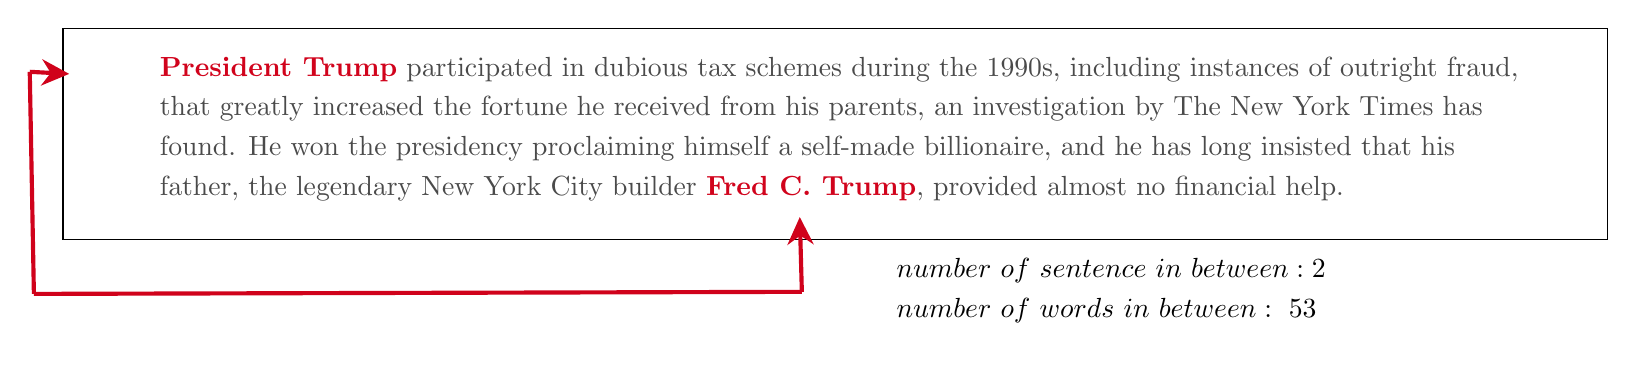
\begin{tikzpicture}[x=0.75pt,y=0.75pt,yscale=-1,xscale=1]
%uncomment if require: \path (0,300); %set diagram left start at 0, and has height of 300

%Shape: Rectangle [id:dp04377104671850285] 
\draw   (28,32) -- (772,32) -- (772,134) -- (28,134) -- cycle ;
%Straight Lines [id:da6182552655813487] 
\draw [color={rgb, 255:red, 208; green, 2; blue, 27 }  ,draw opacity=1 ][line width=1.5]    (28,53.84) -- (12,53) ;

\draw [shift={(31,54)}, rotate = 183.01] [fill={rgb, 255:red, 208; green, 2; blue, 27 }  ,fill opacity=1 ][line width=1.5]  [draw opacity=0] (13.4,-6.43) -- (0,0) -- (13.4,6.44) -- (8.9,0) -- cycle    ;
%Straight Lines [id:da6143692538402417] 
\draw [color={rgb, 255:red, 208; green, 2; blue, 27 }  ,draw opacity=1 ][line width=1.5]    (12,53) -- (14,160) ;


%Straight Lines [id:da10338493648199298] 
\draw [color={rgb, 255:red, 208; green, 2; blue, 27 }  ,draw opacity=1 ][line width=1.5]    (384,159) -- (14,160) ;


%Straight Lines [id:da054560662392693526] 
\draw [color={rgb, 255:red, 208; green, 2; blue, 27 }  ,draw opacity=1 ][line width=1.5]    (383.08,126) -- (384,159) ;

\draw [shift={(383,123)}, rotate = 88.41] [fill={rgb, 255:red, 208; green, 2; blue, 27 }  ,fill opacity=1 ][line width=1.5]  [draw opacity=0] (13.4,-6.43) -- (0,0) -- (13.4,6.44) -- (8.9,0) -- cycle    ;

% Text Node
\draw (402,108) node [scale=1,color={rgb, 255:red, 74; green, 74; blue, 74 }  ,opacity=1 ] [align=left] {\textcolor[rgb]{0.82,0.01,0.11}{\textbf{President Trump}} participated in dubious tax schemes during the 1990s, including instances of outright fraud, \\that greatly increased the fortune he received from his parents, an investigation by The New York Times has\\found. He won the presidency proclaiming himself a self-made billionaire, and he has long insisted that his \\father, the legendary New York City builder \textcolor[rgb]{0.82,0.01,0.11}{\textbf{Fred C. Trump}}, provided almost no financial help.\\\\\\};
% Text Node
\draw (533,158) node   {$ \begin{array}{l}
number\ of\ sentence\ in\ between:2\\
number\ of\ words\ in\ between:\ 53
\end{array}$};


\end{tikzpicture}

}
\caption{An example text to show the relation between two actor entities, \emph{``Donald Trump"} and \emph{``Fred C. Trump"}. If the word-based window size is applied then the relationships between the two entities is not captured, even though they are only one sentence apart. }
\label{fig:article_entities}
\end{figure}
\noindent
We defined a co-occurrence graph of words in Chapter~\ref{chap:background}, as a graph $G=(T,E)$, where $T$ is the set of terms in the vocabulary as nodes and $E$ set of edges and the edge weights encode some notion of distance between the words. We extract such graph from the textual corpus with named entity annotations. As a result, we obtain a weighted heterogeneous graph $G=(N\bigcup  \acute {N},E)$ of named entities and terms, where the set $N$ contains entities of different types and $ \acute {N }$ denotes all the words which are not a named entity (terms). For entity annotations in particular, co-occurence graphs, which are implicitely extracte from text, such as LOAD, can serve as graph representations. By using stenece-window for finding the relationship between entities, they can capture entity relations even stentences apart. ~\brackettext{\cite{DBLP:conf/sigir/SpitzG16}}. Thus, by embedding the nodes, we can obtain word embeddings for both terms and entities.  We later show that this method achieves a better performance in comparison to $a$W2V and $a$GLV on the annotated text. For the node embeddings, we chose DeepWalk (DW)~\footnote{Our model is an adoption of the DeepWalk package in python: https://github.com/phanein/deepwalk} and VERSE (VRS)~\footnote{VERSE package is available in C++: https://github.com/xgfs/verse}, explained in Chapter~\ref{chap:background}, Sections~\ref{subsec:DeepWalk} and ~\ref{subsec:VERSE} respectively. However, since we work on weighted graphs and weights display the strength of the relationships, weighted random walks are introduced to replace the uniform random walk in the DeepWalk model. The probability of a node visiting its neighbors is proportional to the edge weight. As a result, the probability of visiting node $j$ from vertex $i$ with edge weight $e_{i,j}$,  is given in Equation~\ref{eq:edge_weight}, where $ E_{ i }$ denotes the set of all edges starting from node $t_{i}$. The stronger the relationship, the more probable is it to be visited. The function $f$ is our \emph{normalization function}. 
\begin{equation}
P_{i,j}=\frac{f(e_{i,j})}{\sum _{ f(e_ k )\in E_{ i } }^{  }{ f(e_k) } }
\label{eq:edge_weight}
\end{equation}
In a word co-occurrence
graph, some words co-occur many times and some only a few times. Therefore, the weights can fluctuate between small numbers up to tens of thousands, resulting in highly unbalanced transition probabilities, causing some nodes to never be visited in a random walk. The weighted degree distribution for LOAD graph as an example is shown is Figure~\ref{fig:degrees}. To solve this issue and create a more balanced weight distribution, we use different normalization functions:

\begin{figure}
\centering 
\resizebox{0.6\textwidth}{0.6\textwidth}{      

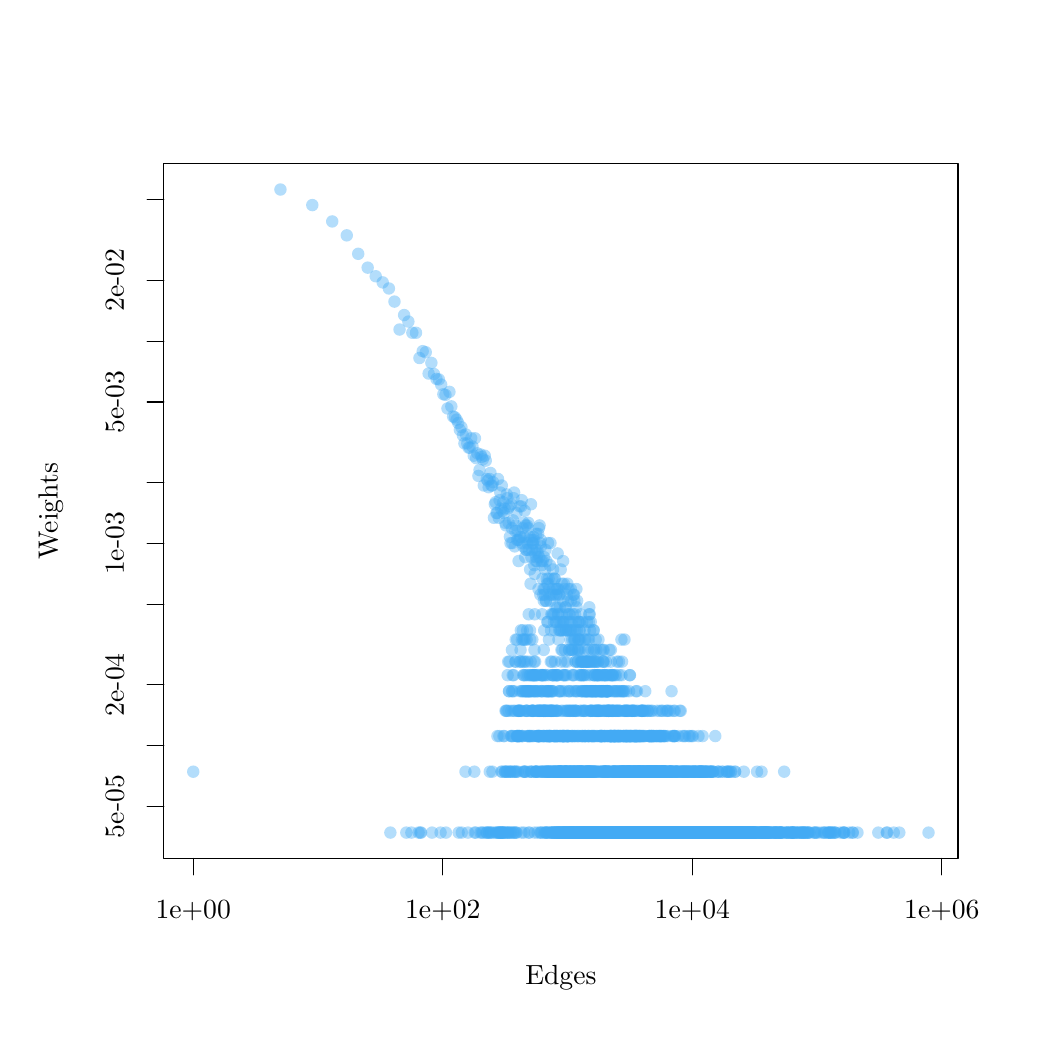
\begin{tikzpicture}[x=1pt,y=1pt]
\definecolor{fillColor}{RGB}{255,255,255}
\path[use as bounding box,fill=fillColor,fill opacity=0.00] (0,0) rectangle (361.35,361.35);
\begin{scope}
\path[clip] ( 49.20, 61.20) rectangle (336.15,312.15);
\definecolor{fillColor}{RGB}{66,170,244}

\path[fill=fillColor,fill opacity=0.40] ( 59.83, 92.50) circle (  2.25);

\path[fill=fillColor,fill opacity=0.40] ( 91.34,302.86) circle (  2.25);

\path[fill=fillColor,fill opacity=0.40] (102.85,297.24) circle (  2.25);

\path[fill=fillColor,fill opacity=0.40] (110.05,291.33) circle (  2.25);

\path[fill=fillColor,fill opacity=0.40] (115.31,286.30) circle (  2.25);

\path[fill=fillColor,fill opacity=0.40] (119.44,279.63) circle (  2.25);

\path[fill=fillColor,fill opacity=0.40] (122.86,274.63) circle (  2.25);

\path[fill=fillColor,fill opacity=0.40] (125.76,271.52) circle (  2.25);

\path[fill=fillColor,fill opacity=0.40] (128.29,269.30) circle (  2.25);

\path[fill=fillColor,fill opacity=0.40] (130.53,267.11) circle (  2.25);

\path[fill=fillColor,fill opacity=0.40] (131.06, 70.49) circle (  2.25);

\path[fill=fillColor,fill opacity=0.40] (132.54,262.37) circle (  2.25);

\path[fill=fillColor,fill opacity=0.40] (134.37,252.27) circle (  2.25);

\path[fill=fillColor,fill opacity=0.40] (136.03,257.50) circle (  2.25);

\path[fill=fillColor,fill opacity=0.40] (136.82, 70.49) circle (  2.25);

\path[fill=fillColor,fill opacity=0.40] (137.57,255.14) circle (  2.25);

\path[fill=fillColor,fill opacity=0.40] (138.65, 70.49) circle (  2.25);

\path[fill=fillColor,fill opacity=0.40] (139.00,251.11) circle (  2.25);

\path[fill=fillColor,fill opacity=0.40] (140.32,251.11) circle (  2.25);

\path[fill=fillColor,fill opacity=0.40] (141.26, 70.49) circle (  2.25);

\path[fill=fillColor,fill opacity=0.40] (141.57,241.98) circle (  2.25);

\path[fill=fillColor,fill opacity=0.40] (141.87, 70.49) circle (  2.25);

\path[fill=fillColor,fill opacity=0.40] (142.16, 70.49) circle (  2.25);

\path[fill=fillColor,fill opacity=0.40] (142.74,244.46) circle (  2.25);

\path[fill=fillColor,fill opacity=0.40] (143.84,244.06) circle (  2.25);

\path[fill=fillColor,fill opacity=0.40] (144.88,236.37) circle (  2.25);

\path[fill=fillColor,fill opacity=0.40] (145.88,240.22) circle (  2.25);

\path[fill=fillColor,fill opacity=0.40] (146.12, 70.49) circle (  2.25);

\path[fill=fillColor,fill opacity=0.40] (146.82,236.19) circle (  2.25);

\path[fill=fillColor,fill opacity=0.40] (147.72,234.43) circle (  2.25);

\path[fill=fillColor,fill opacity=0.40] (148.58,234.25) circle (  2.25);

\path[fill=fillColor,fill opacity=0.40] (149.20, 70.49) circle (  2.25);

\path[fill=fillColor,fill opacity=0.40] (149.41,232.37) circle (  2.25);

\path[fill=fillColor,fill opacity=0.40] (150.20,228.90) circle (  2.25);

\path[fill=fillColor,fill opacity=0.40] (150.96,228.68) circle (  2.25);

\path[fill=fillColor,fill opacity=0.40] (151.14, 70.49) circle (  2.25);

\path[fill=fillColor,fill opacity=0.40] (151.69,223.75) circle (  2.25);

\path[fill=fillColor,fill opacity=0.40] (152.40,229.75) circle (  2.25);

\path[fill=fillColor,fill opacity=0.40] (153.08,224.50) circle (  2.25);

\path[fill=fillColor,fill opacity=0.40] (153.74,220.83) circle (  2.25);

\path[fill=fillColor,fill opacity=0.40] (154.37,220.55) circle (  2.25);

\path[fill=fillColor,fill opacity=0.40] (154.99,219.69) circle (  2.25);

\path[fill=fillColor,fill opacity=0.40] (155.59,218.52) circle (  2.25);

\path[fill=fillColor,fill opacity=0.40] (155.73, 70.49) circle (  2.25);

\path[fill=fillColor,fill opacity=0.40] (156.17,216.03) circle (  2.25);

\path[fill=fillColor,fill opacity=0.40] (156.73,216.98) circle (  2.25);

\path[fill=fillColor,fill opacity=0.40] (156.87, 70.49) circle (  2.25);

\path[fill=fillColor,fill opacity=0.40] (157.28,214.02) circle (  2.25);

\path[fill=fillColor,fill opacity=0.40] (157.81,211.13) circle (  2.25);

\path[fill=fillColor,fill opacity=0.40] (158.20, 92.50) circle (  2.25);

\path[fill=fillColor,fill opacity=0.40] (158.33,214.36) circle (  2.25);

\path[fill=fillColor,fill opacity=0.40] (158.84,211.13) circle (  2.25);

\path[fill=fillColor,fill opacity=0.40] (159.08, 70.49) circle (  2.25);

\path[fill=fillColor,fill opacity=0.40] (159.33,209.58) circle (  2.25);

\path[fill=fillColor,fill opacity=0.40] (159.81,209.58) circle (  2.25);

\path[fill=fillColor,fill opacity=0.40] (160.28,212.97) circle (  2.25);

\path[fill=fillColor,fill opacity=0.40] (160.74,209.98) circle (  2.25);

\path[fill=fillColor,fill opacity=0.40] (161.18,206.68) circle (  2.25);

\path[fill=fillColor,fill opacity=0.40] (161.40, 92.50) circle (  2.25);

\path[fill=fillColor,fill opacity=0.40] (161.51, 70.49) circle (  2.25);

\path[fill=fillColor,fill opacity=0.40] (161.62,212.97) circle (  2.25);

\path[fill=fillColor,fill opacity=0.40] (161.94, 70.49) circle (  2.25);

\path[fill=fillColor,fill opacity=0.40] (162.05,205.80) circle (  2.25);

\path[fill=fillColor,fill opacity=0.40] (162.47,207.54) circle (  2.25);

\path[fill=fillColor,fill opacity=0.40] (162.88,199.38) circle (  2.25);

\path[fill=fillColor,fill opacity=0.40] (163.28,201.49) circle (  2.25);

\path[fill=fillColor,fill opacity=0.40] (163.58, 70.49) circle (  2.25);

\path[fill=fillColor,fill opacity=0.40] (163.67,207.11) circle (  2.25);

\path[fill=fillColor,fill opacity=0.40] (164.06,206.24) circle (  2.25);

\path[fill=fillColor,fill opacity=0.40] (164.15, 70.49) circle (  2.25);

\path[fill=fillColor,fill opacity=0.40] (164.44,205.35) circle (  2.25);

\path[fill=fillColor,fill opacity=0.40] (164.62, 70.49) circle (  2.25);

\path[fill=fillColor,fill opacity=0.40] (164.81,195.91) circle (  2.25);

\path[fill=fillColor,fill opacity=0.40] (165.17,206.68) circle (  2.25);

\path[fill=fillColor,fill opacity=0.40] (165.53,204.89) circle (  2.25);

\path[fill=fillColor,fill opacity=0.40] (165.62, 70.49) circle (  2.25);

\path[fill=fillColor,fill opacity=0.40] (165.88,198.26) circle (  2.25);

\path[fill=fillColor,fill opacity=0.40] (165.97, 70.49) circle (  2.25);

\path[fill=fillColor,fill opacity=0.40] (166.05, 70.49) circle (  2.25);

\path[fill=fillColor,fill opacity=0.40] (166.23,197.69) circle (  2.25);

\path[fill=fillColor,fill opacity=0.40] (166.57,195.29) circle (  2.25);

\path[fill=fillColor,fill opacity=0.40] (166.65, 70.49) circle (  2.25);

\path[fill=fillColor,fill opacity=0.40] (166.73, 70.49) circle (  2.25);

\path[fill=fillColor,fill opacity=0.40] (166.90,198.26) circle (  2.25);

\path[fill=fillColor,fill opacity=0.40] (166.98, 92.50) circle (  2.25);

\path[fill=fillColor,fill opacity=0.40] (167.23,200.45) circle (  2.25);

\path[fill=fillColor,fill opacity=0.40] (167.31, 70.49) circle (  2.25);

\path[fill=fillColor,fill opacity=0.40] (167.47, 70.49) circle (  2.25);

\path[fill=fillColor,fill opacity=0.40] (167.55,195.91) circle (  2.25);

\path[fill=fillColor,fill opacity=0.40] (167.87,195.91) circle (  2.25);

\path[fill=fillColor,fill opacity=0.40] (167.94, 92.50) circle (  2.25);

\path[fill=fillColor,fill opacity=0.40] (168.18,197.11) circle (  2.25);

\path[fill=fillColor,fill opacity=0.40] (168.26, 70.49) circle (  2.25);

\path[fill=fillColor,fill opacity=0.40] (168.49,184.24) circle (  2.25);

\path[fill=fillColor,fill opacity=0.40] (168.79,189.13) circle (  2.25);

\path[fill=fillColor,fill opacity=0.40] (169.09,189.88) circle (  2.25);

\path[fill=fillColor,fill opacity=0.40] (169.23, 70.49) circle (  2.25);

\path[fill=fillColor,fill opacity=0.40] (169.31, 70.49) circle (  2.25);

\path[fill=fillColor,fill opacity=0.40] (169.38,185.96) circle (  2.25);

\path[fill=fillColor,fill opacity=0.40] (169.67,185.96) circle (  2.25);

\path[fill=fillColor,fill opacity=0.40] (169.74,105.37) circle (  2.25);

\path[fill=fillColor,fill opacity=0.40] (169.81, 70.49) circle (  2.25);

\path[fill=fillColor,fill opacity=0.40] (169.95,198.26) circle (  2.25);

\path[fill=fillColor,fill opacity=0.40] (170.16, 70.49) circle (  2.25);

\path[fill=fillColor,fill opacity=0.40] (170.23,184.24) circle (  2.25);

\path[fill=fillColor,fill opacity=0.40] (170.30, 70.49) circle (  2.25);

\path[fill=fillColor,fill opacity=0.40] (170.37, 70.49) circle (  2.25);

\path[fill=fillColor,fill opacity=0.40] (170.44,105.37) circle (  2.25);

\path[fill=fillColor,fill opacity=0.40] (170.51,190.61) circle (  2.25);

\path[fill=fillColor,fill opacity=0.40] (170.58, 70.49) circle (  2.25);

\path[fill=fillColor,fill opacity=0.40] (170.72, 70.49) circle (  2.25);

\path[fill=fillColor,fill opacity=0.40] (170.78,193.37) circle (  2.25);

\path[fill=fillColor,fill opacity=0.40] (170.85, 70.49) circle (  2.25);

\path[fill=fillColor,fill opacity=0.40] (171.05,187.58) circle (  2.25);

\path[fill=fillColor,fill opacity=0.40] (171.19, 92.50) circle (  2.25);

\path[fill=fillColor,fill opacity=0.40] (171.25, 70.49) circle (  2.25);

\path[fill=fillColor,fill opacity=0.40] (171.32,195.91) circle (  2.25);

\path[fill=fillColor,fill opacity=0.40] (171.38, 70.49) circle (  2.25);

\path[fill=fillColor,fill opacity=0.40] (171.45, 92.50) circle (  2.25);

\path[fill=fillColor,fill opacity=0.40] (171.51, 70.49) circle (  2.25);

\path[fill=fillColor,fill opacity=0.40] (171.58,186.78) circle (  2.25);

\path[fill=fillColor,fill opacity=0.40] (171.64, 70.49) circle (  2.25);

\path[fill=fillColor,fill opacity=0.40] (171.71, 70.49) circle (  2.25);

\path[fill=fillColor,fill opacity=0.40] (171.77, 70.49) circle (  2.25);

\path[fill=fillColor,fill opacity=0.40] (171.84,189.88) circle (  2.25);

\path[fill=fillColor,fill opacity=0.40] (171.90,105.37) circle (  2.25);

\path[fill=fillColor,fill opacity=0.40] (172.09,185.96) circle (  2.25);

\path[fill=fillColor,fill opacity=0.40] (172.16, 70.49) circle (  2.25);

\path[fill=fillColor,fill opacity=0.40] (172.28,105.37) circle (  2.25);

\path[fill=fillColor,fill opacity=0.40] (172.35,187.58) circle (  2.25);

\path[fill=fillColor,fill opacity=0.40] (172.41, 92.50) circle (  2.25);

\path[fill=fillColor,fill opacity=0.40] (172.47, 92.50) circle (  2.25);

\path[fill=fillColor,fill opacity=0.40] (172.53, 70.49) circle (  2.25);

\path[fill=fillColor,fill opacity=0.40] (172.59,182.42) circle (  2.25);

\path[fill=fillColor,fill opacity=0.40] (172.66,114.50) circle (  2.25);

\path[fill=fillColor,fill opacity=0.40] (172.72, 92.50) circle (  2.25);

\path[fill=fillColor,fill opacity=0.40] (172.78, 70.49) circle (  2.25);

\path[fill=fillColor,fill opacity=0.40] (172.84,181.48) circle (  2.25);

\path[fill=fillColor,fill opacity=0.40] (172.90,114.50) circle (  2.25);

\path[fill=fillColor,fill opacity=0.40] (173.02, 92.50) circle (  2.25);

\path[fill=fillColor,fill opacity=0.40] (173.08,192.70) circle (  2.25);

\path[fill=fillColor,fill opacity=0.40] (173.14,114.50) circle (  2.25);

\path[fill=fillColor,fill opacity=0.40] (173.26, 92.50) circle (  2.25);

\path[fill=fillColor,fill opacity=0.40] (173.32,191.32) circle (  2.25);

\path[fill=fillColor,fill opacity=0.40] (173.38, 70.49) circle (  2.25);

\path[fill=fillColor,fill opacity=0.40] (173.44,127.37) circle (  2.25);

\path[fill=fillColor,fill opacity=0.40] (173.50, 70.49) circle (  2.25);

\path[fill=fillColor,fill opacity=0.40] (173.56,187.58) circle (  2.25);

\path[fill=fillColor,fill opacity=0.40] (173.62,132.26) circle (  2.25);

\path[fill=fillColor,fill opacity=0.40] (173.68, 70.49) circle (  2.25);

\path[fill=fillColor,fill opacity=0.40] (173.73,114.50) circle (  2.25);

\path[fill=fillColor,fill opacity=0.40] (173.79,182.42) circle (  2.25);

\path[fill=fillColor,fill opacity=0.40] (173.85, 92.50) circle (  2.25);

\path[fill=fillColor,fill opacity=0.40] (173.91,121.58) circle (  2.25);

\path[fill=fillColor,fill opacity=0.40] (173.97,121.58) circle (  2.25);

\path[fill=fillColor,fill opacity=0.40] (174.02,188.37) circle (  2.25);

\path[fill=fillColor,fill opacity=0.40] (174.08,132.26) circle (  2.25);

\path[fill=fillColor,fill opacity=0.40] (174.14, 70.49) circle (  2.25);

\path[fill=fillColor,fill opacity=0.40] (174.25,177.38) circle (  2.25);

\path[fill=fillColor,fill opacity=0.40] (174.31, 92.50) circle (  2.25);

\path[fill=fillColor,fill opacity=0.40] (174.42, 92.50) circle (  2.25);

\path[fill=fillColor,fill opacity=0.40] (174.48,175.11) circle (  2.25);

\path[fill=fillColor,fill opacity=0.40] (174.53, 70.49) circle (  2.25);

\path[fill=fillColor,fill opacity=0.40] (174.59, 92.50) circle (  2.25);

\path[fill=fillColor,fill opacity=0.40] (174.64,105.37) circle (  2.25);

\path[fill=fillColor,fill opacity=0.40] (174.70,189.13) circle (  2.25);

\path[fill=fillColor,fill opacity=0.40] (174.76,114.50) circle (  2.25);

\path[fill=fillColor,fill opacity=0.40] (174.81,105.37) circle (  2.25);

\path[fill=fillColor,fill opacity=0.40] (174.87, 70.49) circle (  2.25);

\path[fill=fillColor,fill opacity=0.40] (174.92,180.50) circle (  2.25);

\path[fill=fillColor,fill opacity=0.40] (174.98,136.50) circle (  2.25);

\path[fill=fillColor,fill opacity=0.40] (175.03,121.58) circle (  2.25);

\path[fill=fillColor,fill opacity=0.40] (175.08,105.37) circle (  2.25);

\path[fill=fillColor,fill opacity=0.40] (175.14,175.11) circle (  2.25);

\path[fill=fillColor,fill opacity=0.40] (175.19,121.58) circle (  2.25);

\path[fill=fillColor,fill opacity=0.40] (175.25,127.37) circle (  2.25);

\path[fill=fillColor,fill opacity=0.40] (175.30, 92.50) circle (  2.25);

\path[fill=fillColor,fill opacity=0.40] (175.35,183.34) circle (  2.25);

\path[fill=fillColor,fill opacity=0.40] (175.41, 70.49) circle (  2.25);

\path[fill=fillColor,fill opacity=0.40] (175.46,105.37) circle (  2.25);

\path[fill=fillColor,fill opacity=0.40] (175.52,114.50) circle (  2.25);

\path[fill=fillColor,fill opacity=0.40] (175.57,191.32) circle (  2.25);

\path[fill=fillColor,fill opacity=0.40] (175.62,127.37) circle (  2.25);

\path[fill=fillColor,fill opacity=0.40] (175.73, 70.49) circle (  2.25);

\path[fill=fillColor,fill opacity=0.40] (175.78,193.37) circle (  2.25);

\path[fill=fillColor,fill opacity=0.40] (175.83,121.58) circle (  2.25);

\path[fill=fillColor,fill opacity=0.40] (175.88, 92.50) circle (  2.25);

\path[fill=fillColor,fill opacity=0.40] (175.94, 92.50) circle (  2.25);

\path[fill=fillColor,fill opacity=0.40] (175.99,173.91) circle (  2.25);

\path[fill=fillColor,fill opacity=0.40] (176.04,114.50) circle (  2.25);

\path[fill=fillColor,fill opacity=0.40] (176.09, 70.49) circle (  2.25);

\path[fill=fillColor,fill opacity=0.40] (176.20,179.49) circle (  2.25);

\path[fill=fillColor,fill opacity=0.40] (176.25,132.26) circle (  2.25);

\path[fill=fillColor,fill opacity=0.40] (176.30,132.26) circle (  2.25);

\path[fill=fillColor,fill opacity=0.40] (176.35,140.24) circle (  2.25);

\path[fill=fillColor,fill opacity=0.40] (176.40,181.48) circle (  2.25);

\path[fill=fillColor,fill opacity=0.40] (176.45, 70.49) circle (  2.25);

\path[fill=fillColor,fill opacity=0.40] (176.50, 92.50) circle (  2.25);

\path[fill=fillColor,fill opacity=0.40] (176.55, 92.50) circle (  2.25);

\path[fill=fillColor,fill opacity=0.40] (176.60,185.96) circle (  2.25);

\path[fill=fillColor,fill opacity=0.40] (176.65, 70.49) circle (  2.25);

\path[fill=fillColor,fill opacity=0.40] (176.70,105.37) circle (  2.25);

\path[fill=fillColor,fill opacity=0.40] (176.75,105.37) circle (  2.25);

\path[fill=fillColor,fill opacity=0.40] (176.80,176.26) circle (  2.25);

\path[fill=fillColor,fill opacity=0.40] (176.85,140.24) circle (  2.25);

\path[fill=fillColor,fill opacity=0.40] (176.90,105.37) circle (  2.25);

\path[fill=fillColor,fill opacity=0.40] (176.95,105.37) circle (  2.25);

\path[fill=fillColor,fill opacity=0.40] (177.00,179.49) circle (  2.25);

\path[fill=fillColor,fill opacity=0.40] (177.05,114.50) circle (  2.25);

\path[fill=fillColor,fill opacity=0.40] (177.10,105.37) circle (  2.25);

\path[fill=fillColor,fill opacity=0.40] (177.15, 92.50) circle (  2.25);

\path[fill=fillColor,fill opacity=0.40] (177.20,176.26) circle (  2.25);

\path[fill=fillColor,fill opacity=0.40] (177.25,105.37) circle (  2.25);

\path[fill=fillColor,fill opacity=0.40] (177.29,114.50) circle (  2.25);

\path[fill=fillColor,fill opacity=0.40] (177.34,114.50) circle (  2.25);

\path[fill=fillColor,fill opacity=0.40] (177.39,168.61) circle (  2.25);

\path[fill=fillColor,fill opacity=0.40] (177.44,114.50) circle (  2.25);

\path[fill=fillColor,fill opacity=0.40] (177.49,105.37) circle (  2.25);

\path[fill=fillColor,fill opacity=0.40] (177.54,114.50) circle (  2.25);

\path[fill=fillColor,fill opacity=0.40] (177.58,176.26) circle (  2.25);

\path[fill=fillColor,fill opacity=0.40] (177.63,105.37) circle (  2.25);

\path[fill=fillColor,fill opacity=0.40] (177.68,105.37) circle (  2.25);

\path[fill=fillColor,fill opacity=0.40] (177.73,114.50) circle (  2.25);

\path[fill=fillColor,fill opacity=0.40] (177.77,188.37) circle (  2.25);

\path[fill=fillColor,fill opacity=0.40] (177.82,132.26) circle (  2.25);

\path[fill=fillColor,fill opacity=0.40] (177.87,105.37) circle (  2.25);

\path[fill=fillColor,fill opacity=0.40] (177.92,114.50) circle (  2.25);

\path[fill=fillColor,fill opacity=0.40] (177.96,177.38) circle (  2.25);

\path[fill=fillColor,fill opacity=0.40] (178.01,121.58) circle (  2.25);

\path[fill=fillColor,fill opacity=0.40] (178.06,132.26) circle (  2.25);

\path[fill=fillColor,fill opacity=0.40] (178.10,136.50) circle (  2.25);

\path[fill=fillColor,fill opacity=0.40] (178.15,177.38) circle (  2.25);

\path[fill=fillColor,fill opacity=0.40] (178.20,143.58) circle (  2.25);

\path[fill=fillColor,fill opacity=0.40] (178.24,114.50) circle (  2.25);

\path[fill=fillColor,fill opacity=0.40] (178.34,188.37) circle (  2.25);

\path[fill=fillColor,fill opacity=0.40] (178.38,114.50) circle (  2.25);

\path[fill=fillColor,fill opacity=0.40] (178.43, 70.49) circle (  2.25);

\path[fill=fillColor,fill opacity=0.40] (178.47,121.58) circle (  2.25);

\path[fill=fillColor,fill opacity=0.40] (178.52,190.61) circle (  2.25);

\path[fill=fillColor,fill opacity=0.40] (178.56,140.24) circle (  2.25);

\path[fill=fillColor,fill opacity=0.40] (178.61,105.37) circle (  2.25);

\path[fill=fillColor,fill opacity=0.40] (178.65,105.37) circle (  2.25);

\path[fill=fillColor,fill opacity=0.40] (178.70,175.11) circle (  2.25);

\path[fill=fillColor,fill opacity=0.40] (178.75,132.26) circle (  2.25);

\path[fill=fillColor,fill opacity=0.40] (178.79,121.58) circle (  2.25);

\path[fill=fillColor,fill opacity=0.40] (178.84,105.37) circle (  2.25);

\path[fill=fillColor,fill opacity=0.40] (178.88,180.50) circle (  2.25);

\path[fill=fillColor,fill opacity=0.40] (178.93,143.58) circle (  2.25);

\path[fill=fillColor,fill opacity=0.40] (178.97,121.58) circle (  2.25);

\path[fill=fillColor,fill opacity=0.40] (179.01, 92.50) circle (  2.25);

\path[fill=fillColor,fill opacity=0.40] (179.06,173.91) circle (  2.25);

\path[fill=fillColor,fill opacity=0.40] (179.10,140.24) circle (  2.25);

\path[fill=fillColor,fill opacity=0.40] (179.15,127.37) circle (  2.25);

\path[fill=fillColor,fill opacity=0.40] (179.19,127.37) circle (  2.25);

\path[fill=fillColor,fill opacity=0.40] (179.24,182.42) circle (  2.25);

\path[fill=fillColor,fill opacity=0.40] (179.28,140.24) circle (  2.25);

\path[fill=fillColor,fill opacity=0.40] (179.32,132.26) circle (  2.25);

\path[fill=fillColor,fill opacity=0.40] (179.37, 70.49) circle (  2.25);

\path[fill=fillColor,fill opacity=0.40] (179.41,177.38) circle (  2.25);

\path[fill=fillColor,fill opacity=0.40] (179.45, 92.50) circle (  2.25);

\path[fill=fillColor,fill opacity=0.40] (179.50,121.58) circle (  2.25);

\path[fill=fillColor,fill opacity=0.40] (179.54, 92.50) circle (  2.25);

\path[fill=fillColor,fill opacity=0.40] (179.58,186.78) circle (  2.25);

\path[fill=fillColor,fill opacity=0.40] (179.63,127.37) circle (  2.25);

\path[fill=fillColor,fill opacity=0.40] (179.67,132.26) circle (  2.25);

\path[fill=fillColor,fill opacity=0.40] (179.71, 92.50) circle (  2.25);

\path[fill=fillColor,fill opacity=0.40] (179.76,170.02) circle (  2.25);

\path[fill=fillColor,fill opacity=0.40] (179.80,140.24) circle (  2.25);

\path[fill=fillColor,fill opacity=0.40] (179.84,121.58) circle (  2.25);

\path[fill=fillColor,fill opacity=0.40] (179.88, 92.50) circle (  2.25);

\path[fill=fillColor,fill opacity=0.40] (179.93,181.48) circle (  2.25);

\path[fill=fillColor,fill opacity=0.40] (179.97,121.58) circle (  2.25);

\path[fill=fillColor,fill opacity=0.40] (180.01,114.50) circle (  2.25);

\path[fill=fillColor,fill opacity=0.40] (180.05,121.58) circle (  2.25);

\path[fill=fillColor,fill opacity=0.40] (180.10,172.66) circle (  2.25);

\path[fill=fillColor,fill opacity=0.40] (180.14,114.50) circle (  2.25);

\path[fill=fillColor,fill opacity=0.40] (180.18,121.58) circle (  2.25);

\path[fill=fillColor,fill opacity=0.40] (180.22,127.37) circle (  2.25);

\path[fill=fillColor,fill opacity=0.40] (180.26,172.66) circle (  2.25);

\path[fill=fillColor,fill opacity=0.40] (180.31,140.24) circle (  2.25);

\path[fill=fillColor,fill opacity=0.40] (180.35,114.50) circle (  2.25);

\path[fill=fillColor,fill opacity=0.40] (180.39,114.50) circle (  2.25);

\path[fill=fillColor,fill opacity=0.40] (180.43,181.48) circle (  2.25);

\path[fill=fillColor,fill opacity=0.40] (180.47,143.58) circle (  2.25);

\path[fill=fillColor,fill opacity=0.40] (180.51,114.50) circle (  2.25);

\path[fill=fillColor,fill opacity=0.40] (180.55,132.26) circle (  2.25);

\path[fill=fillColor,fill opacity=0.40] (180.60,175.11) circle (  2.25);

\path[fill=fillColor,fill opacity=0.40] (180.64,105.37) circle (  2.25);

\path[fill=fillColor,fill opacity=0.40] (180.68,105.37) circle (  2.25);

\path[fill=fillColor,fill opacity=0.40] (180.72,121.58) circle (  2.25);

\path[fill=fillColor,fill opacity=0.40] (180.76,180.50) circle (  2.25);

\path[fill=fillColor,fill opacity=0.40] (180.80,121.58) circle (  2.25);

\path[fill=fillColor,fill opacity=0.40] (180.84,105.37) circle (  2.25);

\path[fill=fillColor,fill opacity=0.40] (180.88,127.37) circle (  2.25);

\path[fill=fillColor,fill opacity=0.40] (180.92,182.42) circle (  2.25);

\path[fill=fillColor,fill opacity=0.40] (180.96, 70.49) circle (  2.25);

\path[fill=fillColor,fill opacity=0.40] (181.00,121.58) circle (  2.25);

\path[fill=fillColor,fill opacity=0.40] (181.04,149.37) circle (  2.25);

\path[fill=fillColor,fill opacity=0.40] (181.08,172.66) circle (  2.25);

\path[fill=fillColor,fill opacity=0.40] (181.12,121.58) circle (  2.25);

\path[fill=fillColor,fill opacity=0.40] (181.16, 92.50) circle (  2.25);

\path[fill=fillColor,fill opacity=0.40] (181.20,105.37) circle (  2.25);

\path[fill=fillColor,fill opacity=0.40] (181.24,176.26) circle (  2.25);

\path[fill=fillColor,fill opacity=0.40] (181.28,121.58) circle (  2.25);

\path[fill=fillColor,fill opacity=0.40] (181.32, 70.49) circle (  2.25);

\path[fill=fillColor,fill opacity=0.40] (181.36,105.37) circle (  2.25);

\path[fill=fillColor,fill opacity=0.40] (181.40,177.38) circle (  2.25);

\path[fill=fillColor,fill opacity=0.40] (181.44,127.37) circle (  2.25);

\path[fill=fillColor,fill opacity=0.40] (181.48,105.37) circle (  2.25);

\path[fill=fillColor,fill opacity=0.40] (181.52,143.58) circle (  2.25);

\path[fill=fillColor,fill opacity=0.40] (181.56,165.58) circle (  2.25);

\path[fill=fillColor,fill opacity=0.40] (181.60,140.24) circle (  2.25);

\path[fill=fillColor,fill opacity=0.40] (181.63,121.58) circle (  2.25);

\path[fill=fillColor,fill opacity=0.40] (181.67,127.37) circle (  2.25);

\path[fill=fillColor,fill opacity=0.40] (181.71,160.42) circle (  2.25);

\path[fill=fillColor,fill opacity=0.40] (181.75,132.26) circle (  2.25);

\path[fill=fillColor,fill opacity=0.40] (181.79,105.37) circle (  2.25);

\path[fill=fillColor,fill opacity=0.40] (181.83,121.58) circle (  2.25);

\path[fill=fillColor,fill opacity=0.40] (181.87,189.13) circle (  2.25);

\path[fill=fillColor,fill opacity=0.40] (181.91,114.50) circle (  2.25);

\path[fill=fillColor,fill opacity=0.40] (181.94, 92.50) circle (  2.25);

\path[fill=fillColor,fill opacity=0.40] (181.98, 92.50) circle (  2.25);

\path[fill=fillColor,fill opacity=0.40] (182.02,170.02) circle (  2.25);

\path[fill=fillColor,fill opacity=0.40] (182.06,105.37) circle (  2.25);

\path[fill=fillColor,fill opacity=0.40] (182.10,121.58) circle (  2.25);

\path[fill=fillColor,fill opacity=0.40] (182.13,114.50) circle (  2.25);

\path[fill=fillColor,fill opacity=0.40] (182.17,176.26) circle (  2.25);

\path[fill=fillColor,fill opacity=0.40] (182.21, 92.50) circle (  2.25);

\path[fill=fillColor,fill opacity=0.40] (182.25,127.37) circle (  2.25);

\path[fill=fillColor,fill opacity=0.40] (182.29,114.50) circle (  2.25);

\path[fill=fillColor,fill opacity=0.40] (182.32,172.66) circle (  2.25);

\path[fill=fillColor,fill opacity=0.40] (182.36,140.24) circle (  2.25);

\path[fill=fillColor,fill opacity=0.40] (182.40,127.37) circle (  2.25);

\path[fill=fillColor,fill opacity=0.40] (182.44,114.50) circle (  2.25);

\path[fill=fillColor,fill opacity=0.40] (182.47,175.11) circle (  2.25);

\path[fill=fillColor,fill opacity=0.40] (182.51,105.37) circle (  2.25);

\path[fill=fillColor,fill opacity=0.40] (182.55,114.50) circle (  2.25);

\path[fill=fillColor,fill opacity=0.40] (182.58,114.50) circle (  2.25);

\path[fill=fillColor,fill opacity=0.40] (182.62,175.11) circle (  2.25);

\path[fill=fillColor,fill opacity=0.40] (182.66,127.37) circle (  2.25);

\path[fill=fillColor,fill opacity=0.40] (182.70,114.50) circle (  2.25);

\path[fill=fillColor,fill opacity=0.40] (182.73,121.58) circle (  2.25);

\path[fill=fillColor,fill opacity=0.40] (182.77,177.38) circle (  2.25);

\path[fill=fillColor,fill opacity=0.40] (182.81,114.50) circle (  2.25);

\path[fill=fillColor,fill opacity=0.40] (182.84,127.37) circle (  2.25);

\path[fill=fillColor,fill opacity=0.40] (182.88,105.37) circle (  2.25);

\path[fill=fillColor,fill opacity=0.40] (182.92,176.26) circle (  2.25);

\path[fill=fillColor,fill opacity=0.40] (182.95,121.58) circle (  2.25);

\path[fill=fillColor,fill opacity=0.40] (182.99,132.26) circle (  2.25);

\path[fill=fillColor,fill opacity=0.40] (183.02,127.37) circle (  2.25);

\path[fill=fillColor,fill opacity=0.40] (183.06,167.13) circle (  2.25);

\path[fill=fillColor,fill opacity=0.40] (183.10,127.37) circle (  2.25);

\path[fill=fillColor,fill opacity=0.40] (183.13,136.50) circle (  2.25);

\path[fill=fillColor,fill opacity=0.40] (183.17, 70.49) circle (  2.25);

\path[fill=fillColor,fill opacity=0.40] (183.20,163.95) circle (  2.25);

\path[fill=fillColor,fill opacity=0.40] (183.24,149.37) circle (  2.25);

\path[fill=fillColor,fill opacity=0.40] (183.28,127.37) circle (  2.25);

\path[fill=fillColor,fill opacity=0.40] (183.35,171.37) circle (  2.25);

\path[fill=fillColor,fill opacity=0.40] (183.38,132.26) circle (  2.25);

\path[fill=fillColor,fill opacity=0.40] (183.42,121.58) circle (  2.25);

\path[fill=fillColor,fill opacity=0.40] (183.45,121.58) circle (  2.25);

\path[fill=fillColor,fill opacity=0.40] (183.49,172.66) circle (  2.25);

\path[fill=fillColor,fill opacity=0.40] (183.53, 92.50) circle (  2.25);

\path[fill=fillColor,fill opacity=0.40] (183.56, 92.50) circle (  2.25);

\path[fill=fillColor,fill opacity=0.40] (183.60, 92.50) circle (  2.25);

\path[fill=fillColor,fill opacity=0.40] (183.63,168.61) circle (  2.25);

\path[fill=fillColor,fill opacity=0.40] (183.67,127.37) circle (  2.25);

\path[fill=fillColor,fill opacity=0.40] (183.70, 92.50) circle (  2.25);

\path[fill=fillColor,fill opacity=0.40] (183.74, 92.50) circle (  2.25);

\path[fill=fillColor,fill opacity=0.40] (183.77,178.45) circle (  2.25);

\path[fill=fillColor,fill opacity=0.40] (183.81,127.37) circle (  2.25);

\path[fill=fillColor,fill opacity=0.40] (183.84,121.58) circle (  2.25);

\path[fill=fillColor,fill opacity=0.40] (183.88, 92.50) circle (  2.25);

\path[fill=fillColor,fill opacity=0.40] (183.91,170.02) circle (  2.25);

\path[fill=fillColor,fill opacity=0.40] (183.95,105.37) circle (  2.25);

\path[fill=fillColor,fill opacity=0.40] (183.98,105.37) circle (  2.25);

\path[fill=fillColor,fill opacity=0.40] (184.01,114.50) circle (  2.25);

\path[fill=fillColor,fill opacity=0.40] (184.05,168.61) circle (  2.25);

\path[fill=fillColor,fill opacity=0.40] (184.08,114.50) circle (  2.25);

\path[fill=fillColor,fill opacity=0.40] (184.12,114.50) circle (  2.25);

\path[fill=fillColor,fill opacity=0.40] (184.15,105.37) circle (  2.25);

\path[fill=fillColor,fill opacity=0.40] (184.19,172.66) circle (  2.25);

\path[fill=fillColor,fill opacity=0.40] (184.22,127.37) circle (  2.25);

\path[fill=fillColor,fill opacity=0.40] (184.25, 70.49) circle (  2.25);

\path[fill=fillColor,fill opacity=0.40] (184.29,121.58) circle (  2.25);

\path[fill=fillColor,fill opacity=0.40] (184.32,171.37) circle (  2.25);

\path[fill=fillColor,fill opacity=0.40] (184.36,105.37) circle (  2.25);

\path[fill=fillColor,fill opacity=0.40] (184.39, 92.50) circle (  2.25);

\path[fill=fillColor,fill opacity=0.40] (184.42,121.58) circle (  2.25);

\path[fill=fillColor,fill opacity=0.40] (184.46,178.45) circle (  2.25);

\path[fill=fillColor,fill opacity=0.40] (184.49,114.50) circle (  2.25);

\path[fill=fillColor,fill opacity=0.40] (184.52,105.37) circle (  2.25);

\path[fill=fillColor,fill opacity=0.40] (184.56,105.37) circle (  2.25);

\path[fill=fillColor,fill opacity=0.40] (184.59,158.50) circle (  2.25);

\path[fill=fillColor,fill opacity=0.40] (184.63,105.37) circle (  2.25);

\path[fill=fillColor,fill opacity=0.40] (184.66,105.37) circle (  2.25);

\path[fill=fillColor,fill opacity=0.40] (184.69,114.50) circle (  2.25);

\path[fill=fillColor,fill opacity=0.40] (184.73,180.50) circle (  2.25);

\path[fill=fillColor,fill opacity=0.40] (184.76,114.50) circle (  2.25);

\path[fill=fillColor,fill opacity=0.40] (184.79,105.37) circle (  2.25);

\path[fill=fillColor,fill opacity=0.40] (184.86,170.02) circle (  2.25);

\path[fill=fillColor,fill opacity=0.40] (184.89,105.37) circle (  2.25);

\path[fill=fillColor,fill opacity=0.40] (184.96,105.37) circle (  2.25);

\path[fill=fillColor,fill opacity=0.40] (184.99,181.48) circle (  2.25);

\path[fill=fillColor,fill opacity=0.40] (185.02,114.50) circle (  2.25);

\path[fill=fillColor,fill opacity=0.40] (185.05,114.50) circle (  2.25);

\path[fill=fillColor,fill opacity=0.40] (185.09, 92.50) circle (  2.25);

\path[fill=fillColor,fill opacity=0.40] (185.12,175.11) circle (  2.25);

\path[fill=fillColor,fill opacity=0.40] (185.15,114.50) circle (  2.25);

\path[fill=fillColor,fill opacity=0.40] (185.19,105.37) circle (  2.25);

\path[fill=fillColor,fill opacity=0.40] (185.25,156.45) circle (  2.25);

\path[fill=fillColor,fill opacity=0.40] (185.28,114.50) circle (  2.25);

\path[fill=fillColor,fill opacity=0.40] (185.31, 70.49) circle (  2.25);

\path[fill=fillColor,fill opacity=0.40] (185.35, 70.49) circle (  2.25);

\path[fill=fillColor,fill opacity=0.40] (185.38,176.26) circle (  2.25);

\path[fill=fillColor,fill opacity=0.40] (185.41,127.37) circle (  2.25);

\path[fill=fillColor,fill opacity=0.40] (185.44, 92.50) circle (  2.25);

\path[fill=fillColor,fill opacity=0.40] (185.48,114.50) circle (  2.25);

\path[fill=fillColor,fill opacity=0.40] (185.51,173.91) circle (  2.25);

\path[fill=fillColor,fill opacity=0.40] (185.54,127.37) circle (  2.25);

\path[fill=fillColor,fill opacity=0.40] (185.57,114.50) circle (  2.25);

\path[fill=fillColor,fill opacity=0.40] (185.60,121.58) circle (  2.25);

\path[fill=fillColor,fill opacity=0.40] (185.63,168.61) circle (  2.25);

\path[fill=fillColor,fill opacity=0.40] (185.67,121.58) circle (  2.25);

\path[fill=fillColor,fill opacity=0.40] (185.70,121.58) circle (  2.25);

\path[fill=fillColor,fill opacity=0.40] (185.73,105.37) circle (  2.25);

\path[fill=fillColor,fill opacity=0.40] (185.76,167.13) circle (  2.25);

\path[fill=fillColor,fill opacity=0.40] (185.79, 92.50) circle (  2.25);

\path[fill=fillColor,fill opacity=0.40] (185.82,127.37) circle (  2.25);

\path[fill=fillColor,fill opacity=0.40] (185.86, 70.49) circle (  2.25);

\path[fill=fillColor,fill opacity=0.40] (185.89,149.37) circle (  2.25);

\path[fill=fillColor,fill opacity=0.40] (185.92,114.50) circle (  2.25);

\path[fill=fillColor,fill opacity=0.40] (185.95, 92.50) circle (  2.25);

\path[fill=fillColor,fill opacity=0.40] (185.98, 92.50) circle (  2.25);

\path[fill=fillColor,fill opacity=0.40] (186.01,162.24) circle (  2.25);

\path[fill=fillColor,fill opacity=0.40] (186.04,127.37) circle (  2.25);

\path[fill=fillColor,fill opacity=0.40] (186.07,105.37) circle (  2.25);

\path[fill=fillColor,fill opacity=0.40] (186.10,121.58) circle (  2.25);

\path[fill=fillColor,fill opacity=0.40] (186.14,168.61) circle (  2.25);

\path[fill=fillColor,fill opacity=0.40] (186.17,127.37) circle (  2.25);

\path[fill=fillColor,fill opacity=0.40] (186.20,127.37) circle (  2.25);

\path[fill=fillColor,fill opacity=0.40] (186.23,105.37) circle (  2.25);

\path[fill=fillColor,fill opacity=0.40] (186.26,156.45) circle (  2.25);

\path[fill=fillColor,fill opacity=0.40] (186.29,114.50) circle (  2.25);

\path[fill=fillColor,fill opacity=0.40] (186.32,114.50) circle (  2.25);

\path[fill=fillColor,fill opacity=0.40] (186.35,114.50) circle (  2.25);

\path[fill=fillColor,fill opacity=0.40] (186.38,158.50) circle (  2.25);

\path[fill=fillColor,fill opacity=0.40] (186.41,114.50) circle (  2.25);

\path[fill=fillColor,fill opacity=0.40] (186.44,114.50) circle (  2.25);

\path[fill=fillColor,fill opacity=0.40] (186.47,136.50) circle (  2.25);

\path[fill=fillColor,fill opacity=0.40] (186.50,154.26) circle (  2.25);

\path[fill=fillColor,fill opacity=0.40] (186.53,105.37) circle (  2.25);

\path[fill=fillColor,fill opacity=0.40] (186.56,105.37) circle (  2.25);

\path[fill=fillColor,fill opacity=0.40] (186.59, 92.50) circle (  2.25);

\path[fill=fillColor,fill opacity=0.40] (186.62,170.02) circle (  2.25);

\path[fill=fillColor,fill opacity=0.40] (186.65,143.58) circle (  2.25);

\path[fill=fillColor,fill opacity=0.40] (186.68,105.37) circle (  2.25);

\path[fill=fillColor,fill opacity=0.40] (186.71, 70.49) circle (  2.25);

\path[fill=fillColor,fill opacity=0.40] (186.74,158.50) circle (  2.25);

\path[fill=fillColor,fill opacity=0.40] (186.77,114.50) circle (  2.25);

\path[fill=fillColor,fill opacity=0.40] (186.80, 92.50) circle (  2.25);

\path[fill=fillColor,fill opacity=0.40] (186.83,114.50) circle (  2.25);

\path[fill=fillColor,fill opacity=0.40] (186.86,156.45) circle (  2.25);

\path[fill=fillColor,fill opacity=0.40] (186.89,114.50) circle (  2.25);

\path[fill=fillColor,fill opacity=0.40] (186.92,121.58) circle (  2.25);

\path[fill=fillColor,fill opacity=0.40] (186.95,114.50) circle (  2.25);

\path[fill=fillColor,fill opacity=0.40] (186.98,165.58) circle (  2.25);

\path[fill=fillColor,fill opacity=0.40] (187.01,127.37) circle (  2.25);

\path[fill=fillColor,fill opacity=0.40] (187.04, 70.49) circle (  2.25);

\path[fill=fillColor,fill opacity=0.40] (187.07, 92.50) circle (  2.25);

\path[fill=fillColor,fill opacity=0.40] (187.10,172.66) circle (  2.25);

\path[fill=fillColor,fill opacity=0.40] (187.13,127.37) circle (  2.25);

\path[fill=fillColor,fill opacity=0.40] (187.16,114.50) circle (  2.25);

\path[fill=fillColor,fill opacity=0.40] (187.19, 92.50) circle (  2.25);

\path[fill=fillColor,fill opacity=0.40] (187.22,154.26) circle (  2.25);

\path[fill=fillColor,fill opacity=0.40] (187.25,114.50) circle (  2.25);

\path[fill=fillColor,fill opacity=0.40] (187.28, 70.49) circle (  2.25);

\path[fill=fillColor,fill opacity=0.40] (187.31,105.37) circle (  2.25);

\path[fill=fillColor,fill opacity=0.40] (187.34,154.26) circle (  2.25);

\path[fill=fillColor,fill opacity=0.40] (187.36,121.58) circle (  2.25);

\path[fill=fillColor,fill opacity=0.40] (187.39, 70.49) circle (  2.25);

\path[fill=fillColor,fill opacity=0.40] (187.42,105.37) circle (  2.25);

\path[fill=fillColor,fill opacity=0.40] (187.45,168.61) circle (  2.25);

\path[fill=fillColor,fill opacity=0.40] (187.48,121.58) circle (  2.25);

\path[fill=fillColor,fill opacity=0.40] (187.51, 92.50) circle (  2.25);

\path[fill=fillColor,fill opacity=0.40] (187.54,114.50) circle (  2.25);

\path[fill=fillColor,fill opacity=0.40] (187.57,162.24) circle (  2.25);

\path[fill=fillColor,fill opacity=0.40] (187.60, 70.49) circle (  2.25);

\path[fill=fillColor,fill opacity=0.40] (187.62, 92.50) circle (  2.25);

\path[fill=fillColor,fill opacity=0.40] (187.65,105.37) circle (  2.25);

\path[fill=fillColor,fill opacity=0.40] (187.68,160.42) circle (  2.25);

\path[fill=fillColor,fill opacity=0.40] (187.71, 92.50) circle (  2.25);

\path[fill=fillColor,fill opacity=0.40] (187.74,114.50) circle (  2.25);

\path[fill=fillColor,fill opacity=0.40] (187.77, 92.50) circle (  2.25);

\path[fill=fillColor,fill opacity=0.40] (187.80,146.61) circle (  2.25);

\path[fill=fillColor,fill opacity=0.40] (187.82,105.37) circle (  2.25);

\path[fill=fillColor,fill opacity=0.40] (187.85, 70.49) circle (  2.25);

\path[fill=fillColor,fill opacity=0.40] (187.88,121.58) circle (  2.25);

\path[fill=fillColor,fill opacity=0.40] (187.91,146.61) circle (  2.25);

\path[fill=fillColor,fill opacity=0.40] (187.94,105.37) circle (  2.25);

\path[fill=fillColor,fill opacity=0.40] (187.97,114.50) circle (  2.25);

\path[fill=fillColor,fill opacity=0.40] (187.99, 92.50) circle (  2.25);

\path[fill=fillColor,fill opacity=0.40] (188.02,175.11) circle (  2.25);

\path[fill=fillColor,fill opacity=0.40] (188.05,121.58) circle (  2.25);

\path[fill=fillColor,fill opacity=0.40] (188.08,121.58) circle (  2.25);

\path[fill=fillColor,fill opacity=0.40] (188.11,114.50) circle (  2.25);

\path[fill=fillColor,fill opacity=0.40] (188.13,160.42) circle (  2.25);

\path[fill=fillColor,fill opacity=0.40] (188.16,105.37) circle (  2.25);

\path[fill=fillColor,fill opacity=0.40] (188.19, 92.50) circle (  2.25);

\path[fill=fillColor,fill opacity=0.40] (188.22,127.37) circle (  2.25);

\path[fill=fillColor,fill opacity=0.40] (188.25,162.24) circle (  2.25);

\path[fill=fillColor,fill opacity=0.40] (188.27, 92.50) circle (  2.25);

\path[fill=fillColor,fill opacity=0.40] (188.30, 92.50) circle (  2.25);

\path[fill=fillColor,fill opacity=0.40] (188.33, 70.49) circle (  2.25);

\path[fill=fillColor,fill opacity=0.40] (188.36,140.24) circle (  2.25);

\path[fill=fillColor,fill opacity=0.40] (188.38,121.58) circle (  2.25);

\path[fill=fillColor,fill opacity=0.40] (188.41,105.37) circle (  2.25);

\path[fill=fillColor,fill opacity=0.40] (188.44,105.37) circle (  2.25);

\path[fill=fillColor,fill opacity=0.40] (188.47,158.50) circle (  2.25);

\path[fill=fillColor,fill opacity=0.40] (188.49,105.37) circle (  2.25);

\path[fill=fillColor,fill opacity=0.40] (188.52,114.50) circle (  2.25);

\path[fill=fillColor,fill opacity=0.40] (188.55,105.37) circle (  2.25);

\path[fill=fillColor,fill opacity=0.40] (188.58,156.45) circle (  2.25);

\path[fill=fillColor,fill opacity=0.40] (188.60,105.37) circle (  2.25);

\path[fill=fillColor,fill opacity=0.40] (188.63, 70.49) circle (  2.25);

\path[fill=fillColor,fill opacity=0.40] (188.66,105.37) circle (  2.25);

\path[fill=fillColor,fill opacity=0.40] (188.68,167.13) circle (  2.25);

\path[fill=fillColor,fill opacity=0.40] (188.71,114.50) circle (  2.25);

\path[fill=fillColor,fill opacity=0.40] (188.74, 92.50) circle (  2.25);

\path[fill=fillColor,fill opacity=0.40] (188.77, 92.50) circle (  2.25);

\path[fill=fillColor,fill opacity=0.40] (188.79,154.26) circle (  2.25);

\path[fill=fillColor,fill opacity=0.40] (188.82,114.50) circle (  2.25);

\path[fill=fillColor,fill opacity=0.40] (188.85,121.58) circle (  2.25);

\path[fill=fillColor,fill opacity=0.40] (188.87, 92.50) circle (  2.25);

\path[fill=fillColor,fill opacity=0.40] (188.90,175.11) circle (  2.25);

\path[fill=fillColor,fill opacity=0.40] (188.93, 92.50) circle (  2.25);

\path[fill=fillColor,fill opacity=0.40] (188.95,114.50) circle (  2.25);

\path[fill=fillColor,fill opacity=0.40] (188.98,105.37) circle (  2.25);

\path[fill=fillColor,fill opacity=0.40] (189.01,132.26) circle (  2.25);

\path[fill=fillColor,fill opacity=0.40] (189.03,105.37) circle (  2.25);

\path[fill=fillColor,fill opacity=0.40] (189.06,121.58) circle (  2.25);

\path[fill=fillColor,fill opacity=0.40] (189.11,143.58) circle (  2.25);

\path[fill=fillColor,fill opacity=0.40] (189.14,114.50) circle (  2.25);

\path[fill=fillColor,fill opacity=0.40] (189.17, 92.50) circle (  2.25);

\path[fill=fillColor,fill opacity=0.40] (189.19,114.50) circle (  2.25);

\path[fill=fillColor,fill opacity=0.40] (189.22,149.37) circle (  2.25);

\path[fill=fillColor,fill opacity=0.40] (189.25,114.50) circle (  2.25);

\path[fill=fillColor,fill opacity=0.40] (189.27, 70.49) circle (  2.25);

\path[fill=fillColor,fill opacity=0.40] (189.30,105.37) circle (  2.25);

\path[fill=fillColor,fill opacity=0.40] (189.33,156.45) circle (  2.25);

\path[fill=fillColor,fill opacity=0.40] (189.35, 70.49) circle (  2.25);

\path[fill=fillColor,fill opacity=0.40] (189.38,114.50) circle (  2.25);

\path[fill=fillColor,fill opacity=0.40] (189.40, 70.49) circle (  2.25);

\path[fill=fillColor,fill opacity=0.40] (189.43,132.26) circle (  2.25);

\path[fill=fillColor,fill opacity=0.40] (189.46,121.58) circle (  2.25);

\path[fill=fillColor,fill opacity=0.40] (189.48, 70.49) circle (  2.25);

\path[fill=fillColor,fill opacity=0.40] (189.51,114.50) circle (  2.25);

\path[fill=fillColor,fill opacity=0.40] (189.54,149.37) circle (  2.25);

\path[fill=fillColor,fill opacity=0.40] (189.56,127.37) circle (  2.25);

\path[fill=fillColor,fill opacity=0.40] (189.59,121.58) circle (  2.25);

\path[fill=fillColor,fill opacity=0.40] (189.61, 92.50) circle (  2.25);

\path[fill=fillColor,fill opacity=0.40] (189.64,162.24) circle (  2.25);

\path[fill=fillColor,fill opacity=0.40] (189.66, 92.50) circle (  2.25);

\path[fill=fillColor,fill opacity=0.40] (189.69,127.37) circle (  2.25);

\path[fill=fillColor,fill opacity=0.40] (189.72,114.50) circle (  2.25);

\path[fill=fillColor,fill opacity=0.40] (189.74,158.50) circle (  2.25);

\path[fill=fillColor,fill opacity=0.40] (189.77,127.37) circle (  2.25);

\path[fill=fillColor,fill opacity=0.40] (189.79, 70.49) circle (  2.25);

\path[fill=fillColor,fill opacity=0.40] (189.82, 70.49) circle (  2.25);

\path[fill=fillColor,fill opacity=0.40] (189.84,165.58) circle (  2.25);

\path[fill=fillColor,fill opacity=0.40] (189.87,121.58) circle (  2.25);

\path[fill=fillColor,fill opacity=0.40] (189.90, 92.50) circle (  2.25);

\path[fill=fillColor,fill opacity=0.40] (189.92,114.50) circle (  2.25);

\path[fill=fillColor,fill opacity=0.40] (189.95,149.37) circle (  2.25);

\path[fill=fillColor,fill opacity=0.40] (190.00,127.37) circle (  2.25);

\path[fill=fillColor,fill opacity=0.40] (190.02,114.50) circle (  2.25);

\path[fill=fillColor,fill opacity=0.40] (190.05,156.45) circle (  2.25);

\path[fill=fillColor,fill opacity=0.40] (190.07,105.37) circle (  2.25);

\path[fill=fillColor,fill opacity=0.40] (190.10, 92.50) circle (  2.25);

\path[fill=fillColor,fill opacity=0.40] (190.12,105.37) circle (  2.25);

\path[fill=fillColor,fill opacity=0.40] (190.15,146.61) circle (  2.25);

\path[fill=fillColor,fill opacity=0.40] (190.17, 92.50) circle (  2.25);

\path[fill=fillColor,fill opacity=0.40] (190.22,105.37) circle (  2.25);

\path[fill=fillColor,fill opacity=0.40] (190.25,149.37) circle (  2.25);

\path[fill=fillColor,fill opacity=0.40] (190.27, 70.49) circle (  2.25);

\path[fill=fillColor,fill opacity=0.40] (190.30, 70.49) circle (  2.25);

\path[fill=fillColor,fill opacity=0.40] (190.33,105.37) circle (  2.25);

\path[fill=fillColor,fill opacity=0.40] (190.35,162.24) circle (  2.25);

\path[fill=fillColor,fill opacity=0.40] (190.37,105.37) circle (  2.25);

\path[fill=fillColor,fill opacity=0.40] (190.40, 92.50) circle (  2.25);

\path[fill=fillColor,fill opacity=0.40] (190.42, 70.49) circle (  2.25);

\path[fill=fillColor,fill opacity=0.40] (190.45,162.24) circle (  2.25);

\path[fill=fillColor,fill opacity=0.40] (190.47,127.37) circle (  2.25);

\path[fill=fillColor,fill opacity=0.40] (190.50, 92.50) circle (  2.25);

\path[fill=fillColor,fill opacity=0.40] (190.52, 70.49) circle (  2.25);

\path[fill=fillColor,fill opacity=0.40] (190.55,143.58) circle (  2.25);

\path[fill=fillColor,fill opacity=0.40] (190.57,132.26) circle (  2.25);

\path[fill=fillColor,fill opacity=0.40] (190.60, 92.50) circle (  2.25);

\path[fill=fillColor,fill opacity=0.40] (190.62,114.50) circle (  2.25);

\path[fill=fillColor,fill opacity=0.40] (190.65,158.50) circle (  2.25);

\path[fill=fillColor,fill opacity=0.40] (190.67, 92.50) circle (  2.25);

\path[fill=fillColor,fill opacity=0.40] (190.70, 92.50) circle (  2.25);

\path[fill=fillColor,fill opacity=0.40] (190.72,105.37) circle (  2.25);

\path[fill=fillColor,fill opacity=0.40] (190.75,151.91) circle (  2.25);

\path[fill=fillColor,fill opacity=0.40] (190.77, 70.49) circle (  2.25);

\path[fill=fillColor,fill opacity=0.40] (190.79,105.37) circle (  2.25);

\path[fill=fillColor,fill opacity=0.40] (190.82,105.37) circle (  2.25);

\path[fill=fillColor,fill opacity=0.40] (190.84,146.61) circle (  2.25);

\path[fill=fillColor,fill opacity=0.40] (190.87, 92.50) circle (  2.25);

\path[fill=fillColor,fill opacity=0.40] (190.89, 70.49) circle (  2.25);

\path[fill=fillColor,fill opacity=0.40] (190.92, 70.49) circle (  2.25);

\path[fill=fillColor,fill opacity=0.40] (190.94,156.45) circle (  2.25);

\path[fill=fillColor,fill opacity=0.40] (190.96,127.37) circle (  2.25);

\path[fill=fillColor,fill opacity=0.40] (190.99, 70.49) circle (  2.25);

\path[fill=fillColor,fill opacity=0.40] (191.04,146.61) circle (  2.25);

\path[fill=fillColor,fill opacity=0.40] (191.06,114.50) circle (  2.25);

\path[fill=fillColor,fill opacity=0.40] (191.08, 70.49) circle (  2.25);

\path[fill=fillColor,fill opacity=0.40] (191.11,127.37) circle (  2.25);

\path[fill=fillColor,fill opacity=0.40] (191.13,156.45) circle (  2.25);

\path[fill=fillColor,fill opacity=0.40] (191.16,105.37) circle (  2.25);

\path[fill=fillColor,fill opacity=0.40] (191.18,114.50) circle (  2.25);

\path[fill=fillColor,fill opacity=0.40] (191.20, 92.50) circle (  2.25);

\path[fill=fillColor,fill opacity=0.40] (191.23,158.50) circle (  2.25);

\path[fill=fillColor,fill opacity=0.40] (191.25,105.37) circle (  2.25);

\path[fill=fillColor,fill opacity=0.40] (191.28,127.37) circle (  2.25);

\path[fill=fillColor,fill opacity=0.40] (191.30,114.50) circle (  2.25);

\path[fill=fillColor,fill opacity=0.40] (191.32,151.91) circle (  2.25);

\path[fill=fillColor,fill opacity=0.40] (191.35,127.37) circle (  2.25);

\path[fill=fillColor,fill opacity=0.40] (191.37,105.37) circle (  2.25);

\path[fill=fillColor,fill opacity=0.40] (191.39, 70.49) circle (  2.25);

\path[fill=fillColor,fill opacity=0.40] (191.42,158.50) circle (  2.25);

\path[fill=fillColor,fill opacity=0.40] (191.44,105.37) circle (  2.25);

\path[fill=fillColor,fill opacity=0.40] (191.47,105.37) circle (  2.25);

\path[fill=fillColor,fill opacity=0.40] (191.49,114.50) circle (  2.25);

\path[fill=fillColor,fill opacity=0.40] (191.51,171.37) circle (  2.25);

\path[fill=fillColor,fill opacity=0.40] (191.54, 70.49) circle (  2.25);

\path[fill=fillColor,fill opacity=0.40] (191.56, 92.50) circle (  2.25);

\path[fill=fillColor,fill opacity=0.40] (191.58, 92.50) circle (  2.25);

\path[fill=fillColor,fill opacity=0.40] (191.61,149.37) circle (  2.25);

\path[fill=fillColor,fill opacity=0.40] (191.63, 92.50) circle (  2.25);

\path[fill=fillColor,fill opacity=0.40] (191.65, 70.49) circle (  2.25);

\path[fill=fillColor,fill opacity=0.40] (191.68,127.37) circle (  2.25);

\path[fill=fillColor,fill opacity=0.40] (191.70,149.37) circle (  2.25);

\path[fill=fillColor,fill opacity=0.40] (191.72, 70.49) circle (  2.25);

\path[fill=fillColor,fill opacity=0.40] (191.75, 70.49) circle (  2.25);

\path[fill=fillColor,fill opacity=0.40] (191.77, 92.50) circle (  2.25);

\path[fill=fillColor,fill opacity=0.40] (191.79,140.24) circle (  2.25);

\path[fill=fillColor,fill opacity=0.40] (191.82, 92.50) circle (  2.25);

\path[fill=fillColor,fill opacity=0.40] (191.84, 92.50) circle (  2.25);

\path[fill=fillColor,fill opacity=0.40] (191.86, 70.49) circle (  2.25);

\path[fill=fillColor,fill opacity=0.40] (191.88,158.50) circle (  2.25);

\path[fill=fillColor,fill opacity=0.40] (191.91, 92.50) circle (  2.25);

\path[fill=fillColor,fill opacity=0.40] (191.93, 70.49) circle (  2.25);

\path[fill=fillColor,fill opacity=0.40] (191.95,121.58) circle (  2.25);

\path[fill=fillColor,fill opacity=0.40] (191.98,156.45) circle (  2.25);

\path[fill=fillColor,fill opacity=0.40] (192.00, 92.50) circle (  2.25);

\path[fill=fillColor,fill opacity=0.40] (192.02,105.37) circle (  2.25);

\path[fill=fillColor,fill opacity=0.40] (192.05, 92.50) circle (  2.25);

\path[fill=fillColor,fill opacity=0.40] (192.07,143.58) circle (  2.25);

\path[fill=fillColor,fill opacity=0.40] (192.09, 70.49) circle (  2.25);

\path[fill=fillColor,fill opacity=0.40] (192.11, 70.49) circle (  2.25);

\path[fill=fillColor,fill opacity=0.40] (192.14, 92.50) circle (  2.25);

\path[fill=fillColor,fill opacity=0.40] (192.16,146.61) circle (  2.25);

\path[fill=fillColor,fill opacity=0.40] (192.18,121.58) circle (  2.25);

\path[fill=fillColor,fill opacity=0.40] (192.20, 92.50) circle (  2.25);

\path[fill=fillColor,fill opacity=0.40] (192.23, 70.49) circle (  2.25);

\path[fill=fillColor,fill opacity=0.40] (192.25,156.45) circle (  2.25);

\path[fill=fillColor,fill opacity=0.40] (192.27, 92.50) circle (  2.25);

\path[fill=fillColor,fill opacity=0.40] (192.30,105.37) circle (  2.25);

\path[fill=fillColor,fill opacity=0.40] (192.32, 70.49) circle (  2.25);

\path[fill=fillColor,fill opacity=0.40] (192.34,151.91) circle (  2.25);

\path[fill=fillColor,fill opacity=0.40] (192.36,105.37) circle (  2.25);

\path[fill=fillColor,fill opacity=0.40] (192.39,121.58) circle (  2.25);

\path[fill=fillColor,fill opacity=0.40] (192.41, 70.49) circle (  2.25);

\path[fill=fillColor,fill opacity=0.40] (192.43,143.58) circle (  2.25);

\path[fill=fillColor,fill opacity=0.40] (192.45, 92.50) circle (  2.25);

\path[fill=fillColor,fill opacity=0.40] (192.48, 92.50) circle (  2.25);

\path[fill=fillColor,fill opacity=0.40] (192.50, 92.50) circle (  2.25);

\path[fill=fillColor,fill opacity=0.40] (192.52,146.61) circle (  2.25);

\path[fill=fillColor,fill opacity=0.40] (192.54, 92.50) circle (  2.25);

\path[fill=fillColor,fill opacity=0.40] (192.56, 92.50) circle (  2.25);

\path[fill=fillColor,fill opacity=0.40] (192.59, 92.50) circle (  2.25);

\path[fill=fillColor,fill opacity=0.40] (192.61,165.58) circle (  2.25);

\path[fill=fillColor,fill opacity=0.40] (192.63, 92.50) circle (  2.25);

\path[fill=fillColor,fill opacity=0.40] (192.65, 70.49) circle (  2.25);

\path[fill=fillColor,fill opacity=0.40] (192.68,105.37) circle (  2.25);

\path[fill=fillColor,fill opacity=0.40] (192.70,143.58) circle (  2.25);

\path[fill=fillColor,fill opacity=0.40] (192.72,105.37) circle (  2.25);

\path[fill=fillColor,fill opacity=0.40] (192.74, 70.49) circle (  2.25);

\path[fill=fillColor,fill opacity=0.40] (192.76, 70.49) circle (  2.25);

\path[fill=fillColor,fill opacity=0.40] (192.79,132.26) circle (  2.25);

\path[fill=fillColor,fill opacity=0.40] (192.81,114.50) circle (  2.25);

\path[fill=fillColor,fill opacity=0.40] (192.85, 92.50) circle (  2.25);

\path[fill=fillColor,fill opacity=0.40] (192.87,136.50) circle (  2.25);

\path[fill=fillColor,fill opacity=0.40] (192.90, 92.50) circle (  2.25);

\path[fill=fillColor,fill opacity=0.40] (192.92, 92.50) circle (  2.25);

\path[fill=fillColor,fill opacity=0.40] (192.94, 92.50) circle (  2.25);

\path[fill=fillColor,fill opacity=0.40] (192.96,149.37) circle (  2.25);

\path[fill=fillColor,fill opacity=0.40] (192.98, 92.50) circle (  2.25);

\path[fill=fillColor,fill opacity=0.40] (193.03, 70.49) circle (  2.25);

\path[fill=fillColor,fill opacity=0.40] (193.05,160.42) circle (  2.25);

\path[fill=fillColor,fill opacity=0.40] (193.07,121.58) circle (  2.25);

\path[fill=fillColor,fill opacity=0.40] (193.09, 92.50) circle (  2.25);

\path[fill=fillColor,fill opacity=0.40] (193.14,143.58) circle (  2.25);

\path[fill=fillColor,fill opacity=0.40] (193.16, 70.49) circle (  2.25);

\path[fill=fillColor,fill opacity=0.40] (193.18,105.37) circle (  2.25);

\path[fill=fillColor,fill opacity=0.40] (193.20,105.37) circle (  2.25);

\path[fill=fillColor,fill opacity=0.40] (193.22,136.50) circle (  2.25);

\path[fill=fillColor,fill opacity=0.40] (193.24,105.37) circle (  2.25);

\path[fill=fillColor,fill opacity=0.40] (193.26, 70.49) circle (  2.25);

\path[fill=fillColor,fill opacity=0.40] (193.29, 70.49) circle (  2.25);

\path[fill=fillColor,fill opacity=0.40] (193.31,146.61) circle (  2.25);

\path[fill=fillColor,fill opacity=0.40] (193.33, 70.49) circle (  2.25);

\path[fill=fillColor,fill opacity=0.40] (193.35,114.50) circle (  2.25);

\path[fill=fillColor,fill opacity=0.40] (193.39,154.26) circle (  2.25);

\path[fill=fillColor,fill opacity=0.40] (193.41,105.37) circle (  2.25);

\path[fill=fillColor,fill opacity=0.40] (193.44, 70.49) circle (  2.25);

\path[fill=fillColor,fill opacity=0.40] (193.46,127.37) circle (  2.25);

\path[fill=fillColor,fill opacity=0.40] (193.48,168.61) circle (  2.25);

\path[fill=fillColor,fill opacity=0.40] (193.50,105.37) circle (  2.25);

\path[fill=fillColor,fill opacity=0.40] (193.52, 92.50) circle (  2.25);

\path[fill=fillColor,fill opacity=0.40] (193.54,105.37) circle (  2.25);

\path[fill=fillColor,fill opacity=0.40] (193.56,146.61) circle (  2.25);

\path[fill=fillColor,fill opacity=0.40] (193.58, 70.49) circle (  2.25);

\path[fill=fillColor,fill opacity=0.40] (193.61, 70.49) circle (  2.25);

\path[fill=fillColor,fill opacity=0.40] (193.63,105.37) circle (  2.25);

\path[fill=fillColor,fill opacity=0.40] (193.65,143.58) circle (  2.25);

\path[fill=fillColor,fill opacity=0.40] (193.67, 92.50) circle (  2.25);

\path[fill=fillColor,fill opacity=0.40] (193.69, 70.49) circle (  2.25);

\path[fill=fillColor,fill opacity=0.40] (193.71, 70.49) circle (  2.25);

\path[fill=fillColor,fill opacity=0.40] (193.73,160.42) circle (  2.25);

\path[fill=fillColor,fill opacity=0.40] (193.75,127.37) circle (  2.25);

\path[fill=fillColor,fill opacity=0.40] (193.77,105.37) circle (  2.25);

\path[fill=fillColor,fill opacity=0.40] (193.79, 70.49) circle (  2.25);

\path[fill=fillColor,fill opacity=0.40] (193.82,146.61) circle (  2.25);

\path[fill=fillColor,fill opacity=0.40] (193.84,105.37) circle (  2.25);

\path[fill=fillColor,fill opacity=0.40] (193.86, 70.49) circle (  2.25);

\path[fill=fillColor,fill opacity=0.40] (193.88, 92.50) circle (  2.25);

\path[fill=fillColor,fill opacity=0.40] (193.90,127.37) circle (  2.25);

\path[fill=fillColor,fill opacity=0.40] (193.92,105.37) circle (  2.25);

\path[fill=fillColor,fill opacity=0.40] (193.94, 92.50) circle (  2.25);

\path[fill=fillColor,fill opacity=0.40] (193.98,158.50) circle (  2.25);

\path[fill=fillColor,fill opacity=0.40] (194.00, 92.50) circle (  2.25);

\path[fill=fillColor,fill opacity=0.40] (194.02, 92.50) circle (  2.25);

\path[fill=fillColor,fill opacity=0.40] (194.04,121.58) circle (  2.25);

\path[fill=fillColor,fill opacity=0.40] (194.07,132.26) circle (  2.25);

\path[fill=fillColor,fill opacity=0.40] (194.09, 92.50) circle (  2.25);

\path[fill=fillColor,fill opacity=0.40] (194.11, 70.49) circle (  2.25);

\path[fill=fillColor,fill opacity=0.40] (194.13,105.37) circle (  2.25);

\path[fill=fillColor,fill opacity=0.40] (194.15,136.50) circle (  2.25);

\path[fill=fillColor,fill opacity=0.40] (194.17, 70.49) circle (  2.25);

\path[fill=fillColor,fill opacity=0.40] (194.19, 70.49) circle (  2.25);

\path[fill=fillColor,fill opacity=0.40] (194.23,151.91) circle (  2.25);

\path[fill=fillColor,fill opacity=0.40] (194.25, 92.50) circle (  2.25);

\path[fill=fillColor,fill opacity=0.40] (194.27, 92.50) circle (  2.25);

\path[fill=fillColor,fill opacity=0.40] (194.29, 92.50) circle (  2.25);

\path[fill=fillColor,fill opacity=0.40] (194.31,127.37) circle (  2.25);

\path[fill=fillColor,fill opacity=0.40] (194.33,114.50) circle (  2.25);

\path[fill=fillColor,fill opacity=0.40] (194.35, 70.49) circle (  2.25);

\path[fill=fillColor,fill opacity=0.40] (194.37,105.37) circle (  2.25);

\path[fill=fillColor,fill opacity=0.40] (194.39,151.91) circle (  2.25);

\path[fill=fillColor,fill opacity=0.40] (194.41, 70.49) circle (  2.25);

\path[fill=fillColor,fill opacity=0.40] (194.43, 92.50) circle (  2.25);

\path[fill=fillColor,fill opacity=0.40] (194.45, 92.50) circle (  2.25);

\path[fill=fillColor,fill opacity=0.40] (194.47,143.58) circle (  2.25);

\path[fill=fillColor,fill opacity=0.40] (194.51, 70.49) circle (  2.25);

\path[fill=fillColor,fill opacity=0.40] (194.53, 70.49) circle (  2.25);

\path[fill=fillColor,fill opacity=0.40] (194.55,143.58) circle (  2.25);

\path[fill=fillColor,fill opacity=0.40] (194.57, 92.50) circle (  2.25);

\path[fill=fillColor,fill opacity=0.40] (194.59, 92.50) circle (  2.25);

\path[fill=fillColor,fill opacity=0.40] (194.61, 70.49) circle (  2.25);

\path[fill=fillColor,fill opacity=0.40] (194.63, 92.50) circle (  2.25);

\path[fill=fillColor,fill opacity=0.40] (194.65,105.37) circle (  2.25);

\path[fill=fillColor,fill opacity=0.40] (194.67, 92.50) circle (  2.25);

\path[fill=fillColor,fill opacity=0.40] (194.69,114.50) circle (  2.25);

\path[fill=fillColor,fill opacity=0.40] (194.71,127.37) circle (  2.25);

\path[fill=fillColor,fill opacity=0.40] (194.73, 92.50) circle (  2.25);

\path[fill=fillColor,fill opacity=0.40] (194.75, 70.49) circle (  2.25);

\path[fill=fillColor,fill opacity=0.40] (194.77, 70.49) circle (  2.25);

\path[fill=fillColor,fill opacity=0.40] (194.79,149.37) circle (  2.25);

\path[fill=fillColor,fill opacity=0.40] (194.81,105.37) circle (  2.25);

\path[fill=fillColor,fill opacity=0.40] (194.83, 92.50) circle (  2.25);

\path[fill=fillColor,fill opacity=0.40] (194.85, 92.50) circle (  2.25);

\path[fill=fillColor,fill opacity=0.40] (194.87,156.45) circle (  2.25);

\path[fill=fillColor,fill opacity=0.40] (194.89,105.37) circle (  2.25);

\path[fill=fillColor,fill opacity=0.40] (194.91, 70.49) circle (  2.25);

\path[fill=fillColor,fill opacity=0.40] (194.93,105.37) circle (  2.25);

\path[fill=fillColor,fill opacity=0.40] (194.95,132.26) circle (  2.25);

\path[fill=fillColor,fill opacity=0.40] (194.97,114.50) circle (  2.25);

\path[fill=fillColor,fill opacity=0.40] (194.99, 92.50) circle (  2.25);

\path[fill=fillColor,fill opacity=0.40] (195.03,160.42) circle (  2.25);

\path[fill=fillColor,fill opacity=0.40] (195.05,105.37) circle (  2.25);

\path[fill=fillColor,fill opacity=0.40] (195.07, 70.49) circle (  2.25);

\path[fill=fillColor,fill opacity=0.40] (195.09,105.37) circle (  2.25);

\path[fill=fillColor,fill opacity=0.40] (195.11,143.58) circle (  2.25);

\path[fill=fillColor,fill opacity=0.40] (195.17, 70.49) circle (  2.25);

\path[fill=fillColor,fill opacity=0.40] (195.19,154.26) circle (  2.25);

\path[fill=fillColor,fill opacity=0.40] (195.21, 92.50) circle (  2.25);

\path[fill=fillColor,fill opacity=0.40] (195.25, 70.49) circle (  2.25);

\path[fill=fillColor,fill opacity=0.40] (195.27,146.61) circle (  2.25);

\path[fill=fillColor,fill opacity=0.40] (195.28,105.37) circle (  2.25);

\path[fill=fillColor,fill opacity=0.40] (195.30,114.50) circle (  2.25);

\path[fill=fillColor,fill opacity=0.40] (195.34,143.58) circle (  2.25);

\path[fill=fillColor,fill opacity=0.40] (195.36, 70.49) circle (  2.25);

\path[fill=fillColor,fill opacity=0.40] (195.38,105.37) circle (  2.25);

\path[fill=fillColor,fill opacity=0.40] (195.40, 70.49) circle (  2.25);

\path[fill=fillColor,fill opacity=0.40] (195.42,158.50) circle (  2.25);

\path[fill=fillColor,fill opacity=0.40] (195.44, 70.49) circle (  2.25);

\path[fill=fillColor,fill opacity=0.40] (195.46,105.37) circle (  2.25);

\path[fill=fillColor,fill opacity=0.40] (195.48, 70.49) circle (  2.25);

\path[fill=fillColor,fill opacity=0.40] (195.50,121.58) circle (  2.25);

\path[fill=fillColor,fill opacity=0.40] (195.52,121.58) circle (  2.25);

\path[fill=fillColor,fill opacity=0.40] (195.54, 92.50) circle (  2.25);

\path[fill=fillColor,fill opacity=0.40] (195.55,105.37) circle (  2.25);

\path[fill=fillColor,fill opacity=0.40] (195.57,136.50) circle (  2.25);

\path[fill=fillColor,fill opacity=0.40] (195.59, 70.49) circle (  2.25);

\path[fill=fillColor,fill opacity=0.40] (195.65,149.37) circle (  2.25);

\path[fill=fillColor,fill opacity=0.40] (195.69, 92.50) circle (  2.25);

\path[fill=fillColor,fill opacity=0.40] (195.73,136.50) circle (  2.25);

\path[fill=fillColor,fill opacity=0.40] (195.74,114.50) circle (  2.25);

\path[fill=fillColor,fill opacity=0.40] (195.76, 92.50) circle (  2.25);

\path[fill=fillColor,fill opacity=0.40] (195.78, 92.50) circle (  2.25);

\path[fill=fillColor,fill opacity=0.40] (195.80,149.37) circle (  2.25);

\path[fill=fillColor,fill opacity=0.40] (195.82, 70.49) circle (  2.25);

\path[fill=fillColor,fill opacity=0.40] (195.84, 70.49) circle (  2.25);

\path[fill=fillColor,fill opacity=0.40] (195.86, 70.49) circle (  2.25);

\path[fill=fillColor,fill opacity=0.40] (195.88, 92.50) circle (  2.25);

\path[fill=fillColor,fill opacity=0.40] (195.90, 70.49) circle (  2.25);

\path[fill=fillColor,fill opacity=0.40] (195.91, 70.49) circle (  2.25);

\path[fill=fillColor,fill opacity=0.40] (195.93, 70.49) circle (  2.25);

\path[fill=fillColor,fill opacity=0.40] (195.95,146.61) circle (  2.25);

\path[fill=fillColor,fill opacity=0.40] (195.97, 92.50) circle (  2.25);

\path[fill=fillColor,fill opacity=0.40] (196.01,114.50) circle (  2.25);

\path[fill=fillColor,fill opacity=0.40] (196.03,140.24) circle (  2.25);

\path[fill=fillColor,fill opacity=0.40] (196.05, 92.50) circle (  2.25);

\path[fill=fillColor,fill opacity=0.40] (196.06,114.50) circle (  2.25);

\path[fill=fillColor,fill opacity=0.40] (196.08, 92.50) circle (  2.25);

\path[fill=fillColor,fill opacity=0.40] (196.10,143.58) circle (  2.25);

\path[fill=fillColor,fill opacity=0.40] (196.14, 92.50) circle (  2.25);

\path[fill=fillColor,fill opacity=0.40] (196.16,105.37) circle (  2.25);

\path[fill=fillColor,fill opacity=0.40] (196.18,121.58) circle (  2.25);

\path[fill=fillColor,fill opacity=0.40] (196.19, 70.49) circle (  2.25);

\path[fill=fillColor,fill opacity=0.40] (196.21, 92.50) circle (  2.25);

\path[fill=fillColor,fill opacity=0.40] (196.23, 70.49) circle (  2.25);

\path[fill=fillColor,fill opacity=0.40] (196.25,158.50) circle (  2.25);

\path[fill=fillColor,fill opacity=0.40] (196.27, 92.50) circle (  2.25);

\path[fill=fillColor,fill opacity=0.40] (196.30, 70.49) circle (  2.25);

\path[fill=fillColor,fill opacity=0.40] (196.32,154.26) circle (  2.25);

\path[fill=fillColor,fill opacity=0.40] (196.34, 70.49) circle (  2.25);

\path[fill=fillColor,fill opacity=0.40] (196.36, 70.49) circle (  2.25);

\path[fill=fillColor,fill opacity=0.40] (196.40,143.58) circle (  2.25);

\path[fill=fillColor,fill opacity=0.40] (196.41, 70.49) circle (  2.25);

\path[fill=fillColor,fill opacity=0.40] (196.43, 70.49) circle (  2.25);

\path[fill=fillColor,fill opacity=0.40] (196.45, 70.49) circle (  2.25);

\path[fill=fillColor,fill opacity=0.40] (196.47,136.50) circle (  2.25);

\path[fill=fillColor,fill opacity=0.40] (196.49, 92.50) circle (  2.25);

\path[fill=fillColor,fill opacity=0.40] (196.51, 92.50) circle (  2.25);

\path[fill=fillColor,fill opacity=0.40] (196.54,146.61) circle (  2.25);

\path[fill=fillColor,fill opacity=0.40] (196.56, 70.49) circle (  2.25);

\path[fill=fillColor,fill opacity=0.40] (196.60, 70.49) circle (  2.25);

\path[fill=fillColor,fill opacity=0.40] (196.62,105.37) circle (  2.25);

\path[fill=fillColor,fill opacity=0.40] (196.63,105.37) circle (  2.25);

\path[fill=fillColor,fill opacity=0.40] (196.65, 70.49) circle (  2.25);

\path[fill=fillColor,fill opacity=0.40] (196.67, 70.49) circle (  2.25);

\path[fill=fillColor,fill opacity=0.40] (196.69,136.50) circle (  2.25);

\path[fill=fillColor,fill opacity=0.40] (196.71, 70.49) circle (  2.25);

\path[fill=fillColor,fill opacity=0.40] (196.72, 70.49) circle (  2.25);

\path[fill=fillColor,fill opacity=0.40] (196.74,114.50) circle (  2.25);

\path[fill=fillColor,fill opacity=0.40] (196.76,140.24) circle (  2.25);

\path[fill=fillColor,fill opacity=0.40] (196.78,114.50) circle (  2.25);

\path[fill=fillColor,fill opacity=0.40] (196.80, 70.49) circle (  2.25);

\path[fill=fillColor,fill opacity=0.40] (196.81, 70.49) circle (  2.25);

\path[fill=fillColor,fill opacity=0.40] (196.83,127.37) circle (  2.25);

\path[fill=fillColor,fill opacity=0.40] (196.85, 70.49) circle (  2.25);

\path[fill=fillColor,fill opacity=0.40] (196.87, 70.49) circle (  2.25);

\path[fill=fillColor,fill opacity=0.40] (196.90,136.50) circle (  2.25);

\path[fill=fillColor,fill opacity=0.40] (196.92,105.37) circle (  2.25);

\path[fill=fillColor,fill opacity=0.40] (196.94, 70.49) circle (  2.25);

\path[fill=fillColor,fill opacity=0.40] (196.96,105.37) circle (  2.25);

\path[fill=fillColor,fill opacity=0.40] (196.97,149.37) circle (  2.25);

\path[fill=fillColor,fill opacity=0.40] (196.99, 92.50) circle (  2.25);

\path[fill=fillColor,fill opacity=0.40] (197.01, 70.49) circle (  2.25);

\path[fill=fillColor,fill opacity=0.40] (197.03, 92.50) circle (  2.25);

\path[fill=fillColor,fill opacity=0.40] (197.05,143.58) circle (  2.25);

\path[fill=fillColor,fill opacity=0.40] (197.06, 92.50) circle (  2.25);

\path[fill=fillColor,fill opacity=0.40] (197.08, 70.49) circle (  2.25);

\path[fill=fillColor,fill opacity=0.40] (197.10, 70.49) circle (  2.25);

\path[fill=fillColor,fill opacity=0.40] (197.12,127.37) circle (  2.25);

\path[fill=fillColor,fill opacity=0.40] (197.13,114.50) circle (  2.25);

\path[fill=fillColor,fill opacity=0.40] (197.15, 92.50) circle (  2.25);

\path[fill=fillColor,fill opacity=0.40] (197.17, 70.49) circle (  2.25);

\path[fill=fillColor,fill opacity=0.40] (197.19,156.45) circle (  2.25);

\path[fill=fillColor,fill opacity=0.40] (197.20, 92.50) circle (  2.25);

\path[fill=fillColor,fill opacity=0.40] (197.22, 70.49) circle (  2.25);

\path[fill=fillColor,fill opacity=0.40] (197.24, 70.49) circle (  2.25);

\path[fill=fillColor,fill opacity=0.40] (197.26,121.58) circle (  2.25);

\path[fill=fillColor,fill opacity=0.40] (197.29, 70.49) circle (  2.25);

\path[fill=fillColor,fill opacity=0.40] (197.31, 70.49) circle (  2.25);

\path[fill=fillColor,fill opacity=0.40] (197.33,140.24) circle (  2.25);

\path[fill=fillColor,fill opacity=0.40] (197.34, 70.49) circle (  2.25);

\path[fill=fillColor,fill opacity=0.40] (197.40,156.45) circle (  2.25);

\path[fill=fillColor,fill opacity=0.40] (197.41,114.50) circle (  2.25);

\path[fill=fillColor,fill opacity=0.40] (197.43, 92.50) circle (  2.25);

\path[fill=fillColor,fill opacity=0.40] (197.45, 92.50) circle (  2.25);

\path[fill=fillColor,fill opacity=0.40] (197.47,127.37) circle (  2.25);

\path[fill=fillColor,fill opacity=0.40] (197.48, 92.50) circle (  2.25);

\path[fill=fillColor,fill opacity=0.40] (197.50,105.37) circle (  2.25);

\path[fill=fillColor,fill opacity=0.40] (197.54,154.26) circle (  2.25);

\path[fill=fillColor,fill opacity=0.40] (197.55, 92.50) circle (  2.25);

\path[fill=fillColor,fill opacity=0.40] (197.59, 70.49) circle (  2.25);

\path[fill=fillColor,fill opacity=0.40] (197.60,140.24) circle (  2.25);

\path[fill=fillColor,fill opacity=0.40] (197.62, 92.50) circle (  2.25);

\path[fill=fillColor,fill opacity=0.40] (197.64,105.37) circle (  2.25);

\path[fill=fillColor,fill opacity=0.40] (197.66, 70.49) circle (  2.25);

\path[fill=fillColor,fill opacity=0.40] (197.67,136.50) circle (  2.25);

\path[fill=fillColor,fill opacity=0.40] (197.69, 92.50) circle (  2.25);

\path[fill=fillColor,fill opacity=0.40] (197.71, 70.49) circle (  2.25);

\path[fill=fillColor,fill opacity=0.40] (197.74,140.24) circle (  2.25);

\path[fill=fillColor,fill opacity=0.40] (197.76, 92.50) circle (  2.25);

\path[fill=fillColor,fill opacity=0.40] (197.79, 92.50) circle (  2.25);

\path[fill=fillColor,fill opacity=0.40] (197.81,149.37) circle (  2.25);

\path[fill=fillColor,fill opacity=0.40] (197.86,105.37) circle (  2.25);

\path[fill=fillColor,fill opacity=0.40] (197.88,143.58) circle (  2.25);

\path[fill=fillColor,fill opacity=0.40] (197.91, 70.49) circle (  2.25);

\path[fill=fillColor,fill opacity=0.40] (197.93, 70.49) circle (  2.25);

\path[fill=fillColor,fill opacity=0.40] (197.95,132.26) circle (  2.25);

\path[fill=fillColor,fill opacity=0.40] (197.96,114.50) circle (  2.25);

\path[fill=fillColor,fill opacity=0.40] (198.00,114.50) circle (  2.25);

\path[fill=fillColor,fill opacity=0.40] (198.01,132.26) circle (  2.25);

\path[fill=fillColor,fill opacity=0.40] (198.05, 70.49) circle (  2.25);

\path[fill=fillColor,fill opacity=0.40] (198.08,146.61) circle (  2.25);

\path[fill=fillColor,fill opacity=0.40] (198.10, 70.49) circle (  2.25);

\path[fill=fillColor,fill opacity=0.40] (198.15,121.58) circle (  2.25);

\path[fill=fillColor,fill opacity=0.40] (198.16,114.50) circle (  2.25);

\path[fill=fillColor,fill opacity=0.40] (198.18, 70.49) circle (  2.25);

\path[fill=fillColor,fill opacity=0.40] (198.21,121.58) circle (  2.25);

\path[fill=fillColor,fill opacity=0.40] (198.23,114.50) circle (  2.25);

\path[fill=fillColor,fill opacity=0.40] (198.26, 70.49) circle (  2.25);

\path[fill=fillColor,fill opacity=0.40] (198.28,158.50) circle (  2.25);

\path[fill=fillColor,fill opacity=0.40] (198.30, 70.49) circle (  2.25);

\path[fill=fillColor,fill opacity=0.40] (198.35,151.91) circle (  2.25);

\path[fill=fillColor,fill opacity=0.40] (198.38, 70.49) circle (  2.25);

\path[fill=fillColor,fill opacity=0.40] (198.40, 70.49) circle (  2.25);

\path[fill=fillColor,fill opacity=0.40] (198.41, 92.50) circle (  2.25);

\path[fill=fillColor,fill opacity=0.40] (198.43, 92.50) circle (  2.25);

\path[fill=fillColor,fill opacity=0.40] (198.45,105.37) circle (  2.25);

\path[fill=fillColor,fill opacity=0.40] (198.48,143.58) circle (  2.25);

\path[fill=fillColor,fill opacity=0.40] (198.50, 92.50) circle (  2.25);

\path[fill=fillColor,fill opacity=0.40] (198.51, 92.50) circle (  2.25);

\path[fill=fillColor,fill opacity=0.40] (198.53, 70.49) circle (  2.25);

\path[fill=fillColor,fill opacity=0.40] (198.55,154.26) circle (  2.25);

\path[fill=fillColor,fill opacity=0.40] (198.58, 92.50) circle (  2.25);

\path[fill=fillColor,fill opacity=0.40] (198.59, 70.49) circle (  2.25);

\path[fill=fillColor,fill opacity=0.40] (198.61,136.50) circle (  2.25);

\path[fill=fillColor,fill opacity=0.40] (198.63, 70.49) circle (  2.25);

\path[fill=fillColor,fill opacity=0.40] (198.66,105.37) circle (  2.25);

\path[fill=fillColor,fill opacity=0.40] (198.68,132.26) circle (  2.25);

\path[fill=fillColor,fill opacity=0.40] (198.69, 92.50) circle (  2.25);

\path[fill=fillColor,fill opacity=0.40] (198.71, 70.49) circle (  2.25);

\path[fill=fillColor,fill opacity=0.40] (198.73, 92.50) circle (  2.25);

\path[fill=fillColor,fill opacity=0.40] (198.74,121.58) circle (  2.25);

\path[fill=fillColor,fill opacity=0.40] (198.77, 92.50) circle (  2.25);

\path[fill=fillColor,fill opacity=0.40] (198.79, 70.49) circle (  2.25);

\path[fill=fillColor,fill opacity=0.40] (198.81,132.26) circle (  2.25);

\path[fill=fillColor,fill opacity=0.40] (198.82, 70.49) circle (  2.25);

\path[fill=fillColor,fill opacity=0.40] (198.84, 70.49) circle (  2.25);

\path[fill=fillColor,fill opacity=0.40] (198.85, 92.50) circle (  2.25);

\path[fill=fillColor,fill opacity=0.40] (198.87,136.50) circle (  2.25);

\path[fill=fillColor,fill opacity=0.40] (198.90, 92.50) circle (  2.25);

\path[fill=fillColor,fill opacity=0.40] (198.94,140.24) circle (  2.25);

\path[fill=fillColor,fill opacity=0.40] (198.95,105.37) circle (  2.25);

\path[fill=fillColor,fill opacity=0.40] (198.97, 70.49) circle (  2.25);

\path[fill=fillColor,fill opacity=0.40] (199.00,146.61) circle (  2.25);

\path[fill=fillColor,fill opacity=0.40] (199.03, 70.49) circle (  2.25);

\path[fill=fillColor,fill opacity=0.40] (199.05, 92.50) circle (  2.25);

\path[fill=fillColor,fill opacity=0.40] (199.06,140.24) circle (  2.25);

\path[fill=fillColor,fill opacity=0.40] (199.13,136.50) circle (  2.25);

\path[fill=fillColor,fill opacity=0.40] (199.14,105.37) circle (  2.25);

\path[fill=fillColor,fill opacity=0.40] (199.16, 70.49) circle (  2.25);

\path[fill=fillColor,fill opacity=0.40] (199.19,146.61) circle (  2.25);

\path[fill=fillColor,fill opacity=0.40] (199.24, 92.50) circle (  2.25);

\path[fill=fillColor,fill opacity=0.40] (199.25,140.24) circle (  2.25);

\path[fill=fillColor,fill opacity=0.40] (199.29, 70.49) circle (  2.25);

\path[fill=fillColor,fill opacity=0.40] (199.32,127.37) circle (  2.25);

\path[fill=fillColor,fill opacity=0.40] (199.35, 70.49) circle (  2.25);

\path[fill=fillColor,fill opacity=0.40] (199.37, 92.50) circle (  2.25);

\path[fill=fillColor,fill opacity=0.40] (199.38,143.58) circle (  2.25);

\path[fill=fillColor,fill opacity=0.40] (199.41, 92.50) circle (  2.25);

\path[fill=fillColor,fill opacity=0.40] (199.43, 92.50) circle (  2.25);

\path[fill=fillColor,fill opacity=0.40] (199.44,143.58) circle (  2.25);

\path[fill=fillColor,fill opacity=0.40] (199.46, 70.49) circle (  2.25);

\path[fill=fillColor,fill opacity=0.40] (199.48, 70.49) circle (  2.25);

\path[fill=fillColor,fill opacity=0.40] (199.49, 70.49) circle (  2.25);

\path[fill=fillColor,fill opacity=0.40] (199.51,146.61) circle (  2.25);

\path[fill=fillColor,fill opacity=0.40] (199.52, 92.50) circle (  2.25);

\path[fill=fillColor,fill opacity=0.40] (199.55, 70.49) circle (  2.25);

\path[fill=fillColor,fill opacity=0.40] (199.57,136.50) circle (  2.25);

\path[fill=fillColor,fill opacity=0.40] (199.58, 70.49) circle (  2.25);

\path[fill=fillColor,fill opacity=0.40] (199.62,105.37) circle (  2.25);

\path[fill=fillColor,fill opacity=0.40] (199.63,114.50) circle (  2.25);

\path[fill=fillColor,fill opacity=0.40] (199.65, 92.50) circle (  2.25);

\path[fill=fillColor,fill opacity=0.40] (199.66, 92.50) circle (  2.25);

\path[fill=fillColor,fill opacity=0.40] (199.68, 92.50) circle (  2.25);

\path[fill=fillColor,fill opacity=0.40] (199.69,140.24) circle (  2.25);

\path[fill=fillColor,fill opacity=0.40] (199.71, 70.49) circle (  2.25);

\path[fill=fillColor,fill opacity=0.40] (199.75,132.26) circle (  2.25);

\path[fill=fillColor,fill opacity=0.40] (199.77, 92.50) circle (  2.25);

\path[fill=fillColor,fill opacity=0.40] (199.79, 70.49) circle (  2.25);

\path[fill=fillColor,fill opacity=0.40] (199.80,121.58) circle (  2.25);

\path[fill=fillColor,fill opacity=0.40] (199.82,127.37) circle (  2.25);

\path[fill=fillColor,fill opacity=0.40] (199.85, 70.49) circle (  2.25);

\path[fill=fillColor,fill opacity=0.40] (199.86, 70.49) circle (  2.25);

\path[fill=fillColor,fill opacity=0.40] (199.88,149.37) circle (  2.25);

\path[fill=fillColor,fill opacity=0.40] (199.91, 70.49) circle (  2.25);

\path[fill=fillColor,fill opacity=0.40] (199.94,114.50) circle (  2.25);

\path[fill=fillColor,fill opacity=0.40] (199.95, 70.49) circle (  2.25);

\path[fill=fillColor,fill opacity=0.40] (199.98, 70.49) circle (  2.25);

\path[fill=fillColor,fill opacity=0.40] (200.00,127.37) circle (  2.25);

\path[fill=fillColor,fill opacity=0.40] (200.02, 92.50) circle (  2.25);

\path[fill=fillColor,fill opacity=0.40] (200.06,132.26) circle (  2.25);

\path[fill=fillColor,fill opacity=0.40] (200.08, 92.50) circle (  2.25);

\path[fill=fillColor,fill opacity=0.40] (200.09, 92.50) circle (  2.25);

\path[fill=fillColor,fill opacity=0.40] (200.11, 70.49) circle (  2.25);

\path[fill=fillColor,fill opacity=0.40] (200.12,132.26) circle (  2.25);

\path[fill=fillColor,fill opacity=0.40] (200.14,105.37) circle (  2.25);

\path[fill=fillColor,fill opacity=0.40] (200.18,127.37) circle (  2.25);

\path[fill=fillColor,fill opacity=0.40] (200.20, 92.50) circle (  2.25);

\path[fill=fillColor,fill opacity=0.40] (200.21, 70.49) circle (  2.25);

\path[fill=fillColor,fill opacity=0.40] (200.24,121.58) circle (  2.25);

\path[fill=fillColor,fill opacity=0.40] (200.26, 92.50) circle (  2.25);

\path[fill=fillColor,fill opacity=0.40] (200.27, 92.50) circle (  2.25);

\path[fill=fillColor,fill opacity=0.40] (200.29, 70.49) circle (  2.25);

\path[fill=fillColor,fill opacity=0.40] (200.30,121.58) circle (  2.25);

\path[fill=fillColor,fill opacity=0.40] (200.32,105.37) circle (  2.25);

\path[fill=fillColor,fill opacity=0.40] (200.33, 70.49) circle (  2.25);

\path[fill=fillColor,fill opacity=0.40] (200.35, 70.49) circle (  2.25);

\path[fill=fillColor,fill opacity=0.40] (200.36,132.26) circle (  2.25);

\path[fill=fillColor,fill opacity=0.40] (200.38, 70.49) circle (  2.25);

\path[fill=fillColor,fill opacity=0.40] (200.39, 70.49) circle (  2.25);

\path[fill=fillColor,fill opacity=0.40] (200.41,105.37) circle (  2.25);

\path[fill=fillColor,fill opacity=0.40] (200.42,146.61) circle (  2.25);

\path[fill=fillColor,fill opacity=0.40] (200.44, 70.49) circle (  2.25);

\path[fill=fillColor,fill opacity=0.40] (200.48,132.26) circle (  2.25);

\path[fill=fillColor,fill opacity=0.40] (200.51, 70.49) circle (  2.25);

\path[fill=fillColor,fill opacity=0.40] (200.54,121.58) circle (  2.25);

\path[fill=fillColor,fill opacity=0.40] (200.56, 70.49) circle (  2.25);

\path[fill=fillColor,fill opacity=0.40] (200.57, 92.50) circle (  2.25);

\path[fill=fillColor,fill opacity=0.40] (200.59, 92.50) circle (  2.25);

\path[fill=fillColor,fill opacity=0.40] (200.60,105.37) circle (  2.25);

\path[fill=fillColor,fill opacity=0.40] (200.62, 92.50) circle (  2.25);

\path[fill=fillColor,fill opacity=0.40] (200.63, 70.49) circle (  2.25);

\path[fill=fillColor,fill opacity=0.40] (200.64, 92.50) circle (  2.25);

\path[fill=fillColor,fill opacity=0.40] (200.66,132.26) circle (  2.25);

\path[fill=fillColor,fill opacity=0.40] (200.67, 70.49) circle (  2.25);

\path[fill=fillColor,fill opacity=0.40] (200.70, 70.49) circle (  2.25);

\path[fill=fillColor,fill opacity=0.40] (200.72,114.50) circle (  2.25);

\path[fill=fillColor,fill opacity=0.40] (200.73, 92.50) circle (  2.25);

\path[fill=fillColor,fill opacity=0.40] (200.75, 70.49) circle (  2.25);

\path[fill=fillColor,fill opacity=0.40] (200.76, 70.49) circle (  2.25);

\path[fill=fillColor,fill opacity=0.40] (200.78,127.37) circle (  2.25);

\path[fill=fillColor,fill opacity=0.40] (200.79, 70.49) circle (  2.25);

\path[fill=fillColor,fill opacity=0.40] (200.81, 70.49) circle (  2.25);

\path[fill=fillColor,fill opacity=0.40] (200.82, 70.49) circle (  2.25);

\path[fill=fillColor,fill opacity=0.40] (200.84,127.37) circle (  2.25);

\path[fill=fillColor,fill opacity=0.40] (200.85, 70.49) circle (  2.25);

\path[fill=fillColor,fill opacity=0.40] (200.89,114.50) circle (  2.25);

\path[fill=fillColor,fill opacity=0.40] (200.91, 70.49) circle (  2.25);

\path[fill=fillColor,fill opacity=0.40] (200.95,132.26) circle (  2.25);

\path[fill=fillColor,fill opacity=0.40] (200.97, 70.49) circle (  2.25);

\path[fill=fillColor,fill opacity=0.40] (200.98, 70.49) circle (  2.25);

\path[fill=fillColor,fill opacity=0.40] (201.00, 92.50) circle (  2.25);

\path[fill=fillColor,fill opacity=0.40] (201.01,127.37) circle (  2.25);

\path[fill=fillColor,fill opacity=0.40] (201.02, 70.49) circle (  2.25);

\path[fill=fillColor,fill opacity=0.40] (201.05,105.37) circle (  2.25);

\path[fill=fillColor,fill opacity=0.40] (201.07,114.50) circle (  2.25);

\path[fill=fillColor,fill opacity=0.40] (201.10, 70.49) circle (  2.25);

\path[fill=fillColor,fill opacity=0.40] (201.11, 70.49) circle (  2.25);

\path[fill=fillColor,fill opacity=0.40] (201.13,121.58) circle (  2.25);

\path[fill=fillColor,fill opacity=0.40] (201.15, 70.49) circle (  2.25);

\path[fill=fillColor,fill opacity=0.40] (201.18,140.24) circle (  2.25);

\path[fill=fillColor,fill opacity=0.40] (201.20, 70.49) circle (  2.25);

\path[fill=fillColor,fill opacity=0.40] (201.23, 70.49) circle (  2.25);

\path[fill=fillColor,fill opacity=0.40] (201.24,143.58) circle (  2.25);

\path[fill=fillColor,fill opacity=0.40] (201.25, 70.49) circle (  2.25);

\path[fill=fillColor,fill opacity=0.40] (201.27, 70.49) circle (  2.25);

\path[fill=fillColor,fill opacity=0.40] (201.28,105.37) circle (  2.25);

\path[fill=fillColor,fill opacity=0.40] (201.30,121.58) circle (  2.25);

\path[fill=fillColor,fill opacity=0.40] (201.33, 70.49) circle (  2.25);

\path[fill=fillColor,fill opacity=0.40] (201.35,114.50) circle (  2.25);

\path[fill=fillColor,fill opacity=0.40] (201.37, 70.49) circle (  2.25);

\path[fill=fillColor,fill opacity=0.40] (201.40, 70.49) circle (  2.25);

\path[fill=fillColor,fill opacity=0.40] (201.41,136.50) circle (  2.25);

\path[fill=fillColor,fill opacity=0.40] (201.43, 70.49) circle (  2.25);

\path[fill=fillColor,fill opacity=0.40] (201.44,105.37) circle (  2.25);

\path[fill=fillColor,fill opacity=0.40] (201.47,132.26) circle (  2.25);

\path[fill=fillColor,fill opacity=0.40] (201.50, 92.50) circle (  2.25);

\path[fill=fillColor,fill opacity=0.40] (201.51,105.37) circle (  2.25);

\path[fill=fillColor,fill opacity=0.40] (201.52,121.58) circle (  2.25);

\path[fill=fillColor,fill opacity=0.40] (201.55, 70.49) circle (  2.25);

\path[fill=fillColor,fill opacity=0.40] (201.57, 92.50) circle (  2.25);

\path[fill=fillColor,fill opacity=0.40] (201.58,140.24) circle (  2.25);

\path[fill=fillColor,fill opacity=0.40] (201.59,105.37) circle (  2.25);

\path[fill=fillColor,fill opacity=0.40] (201.61, 70.49) circle (  2.25);

\path[fill=fillColor,fill opacity=0.40] (201.62, 92.50) circle (  2.25);

\path[fill=fillColor,fill opacity=0.40] (201.64,121.58) circle (  2.25);

\path[fill=fillColor,fill opacity=0.40] (201.66, 92.50) circle (  2.25);

\path[fill=fillColor,fill opacity=0.40] (201.68, 70.49) circle (  2.25);

\path[fill=fillColor,fill opacity=0.40] (201.69,132.26) circle (  2.25);

\path[fill=fillColor,fill opacity=0.40] (201.72, 70.49) circle (  2.25);

\path[fill=fillColor,fill opacity=0.40] (201.75,114.50) circle (  2.25);

\path[fill=fillColor,fill opacity=0.40] (201.78, 70.49) circle (  2.25);

\path[fill=fillColor,fill opacity=0.40] (201.79, 92.50) circle (  2.25);

\path[fill=fillColor,fill opacity=0.40] (201.80,121.58) circle (  2.25);

\path[fill=fillColor,fill opacity=0.40] (201.85, 70.49) circle (  2.25);

\path[fill=fillColor,fill opacity=0.40] (201.86,132.26) circle (  2.25);

\path[fill=fillColor,fill opacity=0.40] (201.87, 70.49) circle (  2.25);

\path[fill=fillColor,fill opacity=0.40] (201.91,132.26) circle (  2.25);

\path[fill=fillColor,fill opacity=0.40] (201.93, 92.50) circle (  2.25);

\path[fill=fillColor,fill opacity=0.40] (201.97,127.37) circle (  2.25);

\path[fill=fillColor,fill opacity=0.40] (202.00, 70.49) circle (  2.25);

\path[fill=fillColor,fill opacity=0.40] (202.01, 92.50) circle (  2.25);

\path[fill=fillColor,fill opacity=0.40] (202.03,121.58) circle (  2.25);

\path[fill=fillColor,fill opacity=0.40] (202.04, 92.50) circle (  2.25);

\path[fill=fillColor,fill opacity=0.40] (202.08,146.61) circle (  2.25);

\path[fill=fillColor,fill opacity=0.40] (202.13,121.58) circle (  2.25);

\path[fill=fillColor,fill opacity=0.40] (202.15, 70.49) circle (  2.25);

\path[fill=fillColor,fill opacity=0.40] (202.16, 70.49) circle (  2.25);

\path[fill=fillColor,fill opacity=0.40] (202.18, 92.50) circle (  2.25);

\path[fill=fillColor,fill opacity=0.40] (202.19,132.26) circle (  2.25);

\path[fill=fillColor,fill opacity=0.40] (202.20, 70.49) circle (  2.25);

\path[fill=fillColor,fill opacity=0.40] (202.22, 92.50) circle (  2.25);

\path[fill=fillColor,fill opacity=0.40] (202.23, 70.49) circle (  2.25);

\path[fill=fillColor,fill opacity=0.40] (202.24,132.26) circle (  2.25);

\path[fill=fillColor,fill opacity=0.40] (202.26, 92.50) circle (  2.25);

\path[fill=fillColor,fill opacity=0.40] (202.28, 70.49) circle (  2.25);

\path[fill=fillColor,fill opacity=0.40] (202.30,105.37) circle (  2.25);

\path[fill=fillColor,fill opacity=0.40] (202.31, 70.49) circle (  2.25);

\path[fill=fillColor,fill opacity=0.40] (202.33, 70.49) circle (  2.25);

\path[fill=fillColor,fill opacity=0.40] (202.35,140.24) circle (  2.25);

\path[fill=fillColor,fill opacity=0.40] (202.37, 92.50) circle (  2.25);

\path[fill=fillColor,fill opacity=0.40] (202.41,121.58) circle (  2.25);

\path[fill=fillColor,fill opacity=0.40] (202.42, 70.49) circle (  2.25);

\path[fill=fillColor,fill opacity=0.40] (202.45, 70.49) circle (  2.25);

\path[fill=fillColor,fill opacity=0.40] (202.46,136.50) circle (  2.25);

\path[fill=fillColor,fill opacity=0.40] (202.47, 70.49) circle (  2.25);

\path[fill=fillColor,fill opacity=0.40] (202.49, 70.49) circle (  2.25);

\path[fill=fillColor,fill opacity=0.40] (202.51,105.37) circle (  2.25);

\path[fill=fillColor,fill opacity=0.40] (202.54, 70.49) circle (  2.25);

\path[fill=fillColor,fill opacity=0.40] (202.57,121.58) circle (  2.25);

\path[fill=fillColor,fill opacity=0.40] (202.58, 92.50) circle (  2.25);

\path[fill=fillColor,fill opacity=0.40] (202.59, 92.50) circle (  2.25);

\path[fill=fillColor,fill opacity=0.40] (202.61, 92.50) circle (  2.25);

\path[fill=fillColor,fill opacity=0.40] (202.62,132.26) circle (  2.25);

\path[fill=fillColor,fill opacity=0.40] (202.63, 92.50) circle (  2.25);

\path[fill=fillColor,fill opacity=0.40] (202.66, 70.49) circle (  2.25);

\path[fill=fillColor,fill opacity=0.40] (202.67,132.26) circle (  2.25);

\path[fill=fillColor,fill opacity=0.40] (202.69, 70.49) circle (  2.25);

\path[fill=fillColor,fill opacity=0.40] (202.70,105.37) circle (  2.25);

\path[fill=fillColor,fill opacity=0.40] (202.73,105.37) circle (  2.25);

\path[fill=fillColor,fill opacity=0.40] (202.75, 70.49) circle (  2.25);

\path[fill=fillColor,fill opacity=0.40] (202.78,146.61) circle (  2.25);

\path[fill=fillColor,fill opacity=0.40] (202.82, 70.49) circle (  2.25);

\path[fill=fillColor,fill opacity=0.40] (202.83,140.24) circle (  2.25);

\path[fill=fillColor,fill opacity=0.40] (202.85, 70.49) circle (  2.25);

\path[fill=fillColor,fill opacity=0.40] (202.87, 92.50) circle (  2.25);

\path[fill=fillColor,fill opacity=0.40] (202.89,149.37) circle (  2.25);

\path[fill=fillColor,fill opacity=0.40] (202.90, 92.50) circle (  2.25);

\path[fill=fillColor,fill opacity=0.40] (202.91, 92.50) circle (  2.25);

\path[fill=fillColor,fill opacity=0.40] (202.92, 92.50) circle (  2.25);

\path[fill=fillColor,fill opacity=0.40] (202.94,151.91) circle (  2.25);

\path[fill=fillColor,fill opacity=0.40] (202.95, 92.50) circle (  2.25);

\path[fill=fillColor,fill opacity=0.40] (202.96, 92.50) circle (  2.25);

\path[fill=fillColor,fill opacity=0.40] (202.99,121.58) circle (  2.25);

\path[fill=fillColor,fill opacity=0.40] (203.00, 70.49) circle (  2.25);

\path[fill=fillColor,fill opacity=0.40] (203.02, 70.49) circle (  2.25);

\path[fill=fillColor,fill opacity=0.40] (203.04,132.26) circle (  2.25);

\path[fill=fillColor,fill opacity=0.40] (203.06, 70.49) circle (  2.25);

\path[fill=fillColor,fill opacity=0.40] (203.08,105.37) circle (  2.25);

\path[fill=fillColor,fill opacity=0.40] (203.09,149.37) circle (  2.25);

\path[fill=fillColor,fill opacity=0.40] (203.11, 70.49) circle (  2.25);

\path[fill=fillColor,fill opacity=0.40] (203.15,114.50) circle (  2.25);

\path[fill=fillColor,fill opacity=0.40] (203.16, 70.49) circle (  2.25);

\path[fill=fillColor,fill opacity=0.40] (203.17, 70.49) circle (  2.25);

\path[fill=fillColor,fill opacity=0.40] (203.20,127.37) circle (  2.25);

\path[fill=fillColor,fill opacity=0.40] (203.21, 70.49) circle (  2.25);

\path[fill=fillColor,fill opacity=0.40] (203.22, 70.49) circle (  2.25);

\path[fill=fillColor,fill opacity=0.40] (203.24, 70.49) circle (  2.25);

\path[fill=fillColor,fill opacity=0.40] (203.25,143.58) circle (  2.25);

\path[fill=fillColor,fill opacity=0.40] (203.26, 92.50) circle (  2.25);

\path[fill=fillColor,fill opacity=0.40] (203.29, 70.49) circle (  2.25);

\path[fill=fillColor,fill opacity=0.40] (203.30,121.58) circle (  2.25);

\path[fill=fillColor,fill opacity=0.40] (203.31, 70.49) circle (  2.25);

\path[fill=fillColor,fill opacity=0.40] (203.33, 70.49) circle (  2.25);

\path[fill=fillColor,fill opacity=0.40] (203.35,114.50) circle (  2.25);

\path[fill=fillColor,fill opacity=0.40] (203.38, 70.49) circle (  2.25);

\path[fill=fillColor,fill opacity=0.40] (203.39, 92.50) circle (  2.25);

\path[fill=fillColor,fill opacity=0.40] (203.40,121.58) circle (  2.25);

\path[fill=fillColor,fill opacity=0.40] (203.43,114.50) circle (  2.25);

\path[fill=fillColor,fill opacity=0.40] (203.44, 70.49) circle (  2.25);

\path[fill=fillColor,fill opacity=0.40] (203.46,146.61) circle (  2.25);

\path[fill=fillColor,fill opacity=0.40] (203.47, 70.49) circle (  2.25);

\path[fill=fillColor,fill opacity=0.40] (203.51,114.50) circle (  2.25);

\path[fill=fillColor,fill opacity=0.40] (203.52, 70.49) circle (  2.25);

\path[fill=fillColor,fill opacity=0.40] (203.53, 92.50) circle (  2.25);

\path[fill=fillColor,fill opacity=0.40] (203.54, 92.50) circle (  2.25);

\path[fill=fillColor,fill opacity=0.40] (203.56,132.26) circle (  2.25);

\path[fill=fillColor,fill opacity=0.40] (203.58, 70.49) circle (  2.25);

\path[fill=fillColor,fill opacity=0.40] (203.61,132.26) circle (  2.25);

\path[fill=fillColor,fill opacity=0.40] (203.62, 92.50) circle (  2.25);

\path[fill=fillColor,fill opacity=0.40] (203.63, 70.49) circle (  2.25);

\path[fill=fillColor,fill opacity=0.40] (203.66,121.58) circle (  2.25);

\path[fill=fillColor,fill opacity=0.40] (203.68,105.37) circle (  2.25);

\path[fill=fillColor,fill opacity=0.40] (203.70, 70.49) circle (  2.25);

\path[fill=fillColor,fill opacity=0.40] (203.71,105.37) circle (  2.25);

\path[fill=fillColor,fill opacity=0.40] (203.73, 70.49) circle (  2.25);

\path[fill=fillColor,fill opacity=0.40] (203.76,136.50) circle (  2.25);

\path[fill=fillColor,fill opacity=0.40] (203.80, 70.49) circle (  2.25);

\path[fill=fillColor,fill opacity=0.40] (203.81,114.50) circle (  2.25);

\path[fill=fillColor,fill opacity=0.40] (203.84, 70.49) circle (  2.25);

\path[fill=fillColor,fill opacity=0.40] (203.85, 92.50) circle (  2.25);

\path[fill=fillColor,fill opacity=0.40] (203.86,121.58) circle (  2.25);

\path[fill=fillColor,fill opacity=0.40] (203.87, 70.49) circle (  2.25);

\path[fill=fillColor,fill opacity=0.40] (203.89, 70.49) circle (  2.25);

\path[fill=fillColor,fill opacity=0.40] (203.90, 92.50) circle (  2.25);

\path[fill=fillColor,fill opacity=0.40] (203.91,121.58) circle (  2.25);

\path[fill=fillColor,fill opacity=0.40] (203.94, 70.49) circle (  2.25);

\path[fill=fillColor,fill opacity=0.40] (203.95, 70.49) circle (  2.25);

\path[fill=fillColor,fill opacity=0.40] (203.96,105.37) circle (  2.25);

\path[fill=fillColor,fill opacity=0.40] (203.97, 70.49) circle (  2.25);

\path[fill=fillColor,fill opacity=0.40] (204.00, 70.49) circle (  2.25);

\path[fill=fillColor,fill opacity=0.40] (204.01,114.50) circle (  2.25);

\path[fill=fillColor,fill opacity=0.40] (204.05, 70.49) circle (  2.25);

\path[fill=fillColor,fill opacity=0.40] (204.06,132.26) circle (  2.25);

\path[fill=fillColor,fill opacity=0.40] (204.07, 70.49) circle (  2.25);

\path[fill=fillColor,fill opacity=0.40] (204.11,121.58) circle (  2.25);

\path[fill=fillColor,fill opacity=0.40] (204.13, 70.49) circle (  2.25);

\path[fill=fillColor,fill opacity=0.40] (204.15, 92.50) circle (  2.25);

\path[fill=fillColor,fill opacity=0.40] (204.16,114.50) circle (  2.25);

\path[fill=fillColor,fill opacity=0.40] (204.21,127.37) circle (  2.25);

\path[fill=fillColor,fill opacity=0.40] (204.23,105.37) circle (  2.25);

\path[fill=fillColor,fill opacity=0.40] (204.24, 92.50) circle (  2.25);

\path[fill=fillColor,fill opacity=0.40] (204.26,121.58) circle (  2.25);

\path[fill=fillColor,fill opacity=0.40] (204.27, 92.50) circle (  2.25);

\path[fill=fillColor,fill opacity=0.40] (204.31,105.37) circle (  2.25);

\path[fill=fillColor,fill opacity=0.40] (204.35, 92.50) circle (  2.25);

\path[fill=fillColor,fill opacity=0.40] (204.39, 70.49) circle (  2.25);

\path[fill=fillColor,fill opacity=0.40] (204.40,121.58) circle (  2.25);

\path[fill=fillColor,fill opacity=0.40] (204.42, 70.49) circle (  2.25);

\path[fill=fillColor,fill opacity=0.40] (204.43, 70.49) circle (  2.25);

\path[fill=fillColor,fill opacity=0.40] (204.44, 70.49) circle (  2.25);

\path[fill=fillColor,fill opacity=0.40] (204.45,143.58) circle (  2.25);

\path[fill=fillColor,fill opacity=0.40] (204.48, 70.49) circle (  2.25);

\path[fill=fillColor,fill opacity=0.40] (204.50, 92.50) circle (  2.25);

\path[fill=fillColor,fill opacity=0.40] (204.51, 70.49) circle (  2.25);

\path[fill=fillColor,fill opacity=0.40] (204.52, 70.49) circle (  2.25);

\path[fill=fillColor,fill opacity=0.40] (204.55,143.58) circle (  2.25);

\path[fill=fillColor,fill opacity=0.40] (204.60,136.50) circle (  2.25);

\path[fill=fillColor,fill opacity=0.40] (204.61,105.37) circle (  2.25);

\path[fill=fillColor,fill opacity=0.40] (204.63, 70.49) circle (  2.25);

\path[fill=fillColor,fill opacity=0.40] (204.64,132.26) circle (  2.25);

\path[fill=fillColor,fill opacity=0.40] (204.69,121.58) circle (  2.25);

\path[fill=fillColor,fill opacity=0.40] (204.71, 70.49) circle (  2.25);

\path[fill=fillColor,fill opacity=0.40] (204.72, 70.49) circle (  2.25);

\path[fill=fillColor,fill opacity=0.40] (204.73, 92.50) circle (  2.25);

\path[fill=fillColor,fill opacity=0.40] (204.74,127.37) circle (  2.25);

\path[fill=fillColor,fill opacity=0.40] (204.76, 92.50) circle (  2.25);

\path[fill=fillColor,fill opacity=0.40] (204.78, 70.49) circle (  2.25);

\path[fill=fillColor,fill opacity=0.40] (204.79,136.50) circle (  2.25);

\path[fill=fillColor,fill opacity=0.40] (204.80,105.37) circle (  2.25);

\path[fill=fillColor,fill opacity=0.40] (204.84,127.37) circle (  2.25);

\path[fill=fillColor,fill opacity=0.40] (204.85, 70.49) circle (  2.25);

\path[fill=fillColor,fill opacity=0.40] (204.86, 70.49) circle (  2.25);

\path[fill=fillColor,fill opacity=0.40] (204.88,132.26) circle (  2.25);

\path[fill=fillColor,fill opacity=0.40] (204.91, 70.49) circle (  2.25);

\path[fill=fillColor,fill opacity=0.40] (204.92, 70.49) circle (  2.25);

\path[fill=fillColor,fill opacity=0.40] (204.93,105.37) circle (  2.25);

\path[fill=fillColor,fill opacity=0.40] (204.98,127.37) circle (  2.25);

\path[fill=fillColor,fill opacity=0.40] (204.99, 70.49) circle (  2.25);

\path[fill=fillColor,fill opacity=0.40] (205.01, 92.50) circle (  2.25);

\path[fill=fillColor,fill opacity=0.40] (205.03,114.50) circle (  2.25);

\path[fill=fillColor,fill opacity=0.40] (205.04,114.50) circle (  2.25);

\path[fill=fillColor,fill opacity=0.40] (205.07,121.58) circle (  2.25);

\path[fill=fillColor,fill opacity=0.40] (205.10, 92.50) circle (  2.25);

\path[fill=fillColor,fill opacity=0.40] (205.11, 70.49) circle (  2.25);

\path[fill=fillColor,fill opacity=0.40] (205.12,121.58) circle (  2.25);

\path[fill=fillColor,fill opacity=0.40] (205.13, 70.49) circle (  2.25);

\path[fill=fillColor,fill opacity=0.40] (205.14, 70.49) circle (  2.25);

\path[fill=fillColor,fill opacity=0.40] (205.17,132.26) circle (  2.25);

\path[fill=fillColor,fill opacity=0.40] (205.18, 70.49) circle (  2.25);

\path[fill=fillColor,fill opacity=0.40] (205.21, 92.50) circle (  2.25);

\path[fill=fillColor,fill opacity=0.40] (205.24, 70.49) circle (  2.25);

\path[fill=fillColor,fill opacity=0.40] (205.26,140.24) circle (  2.25);

\path[fill=fillColor,fill opacity=0.40] (205.28,114.50) circle (  2.25);

\path[fill=fillColor,fill opacity=0.40] (205.31,121.58) circle (  2.25);

\path[fill=fillColor,fill opacity=0.40] (205.34, 70.49) circle (  2.25);

\path[fill=fillColor,fill opacity=0.40] (205.35,121.58) circle (  2.25);

\path[fill=fillColor,fill opacity=0.40] (205.40,121.58) circle (  2.25);

\path[fill=fillColor,fill opacity=0.40] (205.42, 92.50) circle (  2.25);

\path[fill=fillColor,fill opacity=0.40] (205.43, 70.49) circle (  2.25);

\path[fill=fillColor,fill opacity=0.40] (205.45,132.26) circle (  2.25);

\path[fill=fillColor,fill opacity=0.40] (205.48, 70.49) circle (  2.25);

\path[fill=fillColor,fill opacity=0.40] (205.49, 70.49) circle (  2.25);

\path[fill=fillColor,fill opacity=0.40] (205.54,136.50) circle (  2.25);

\path[fill=fillColor,fill opacity=0.40] (205.55,105.37) circle (  2.25);

\path[fill=fillColor,fill opacity=0.40] (205.58,114.50) circle (  2.25);

\path[fill=fillColor,fill opacity=0.40] (205.60, 70.49) circle (  2.25);

\path[fill=fillColor,fill opacity=0.40] (205.61, 70.49) circle (  2.25);

\path[fill=fillColor,fill opacity=0.40] (205.63,114.50) circle (  2.25);

\path[fill=fillColor,fill opacity=0.40] (205.65, 70.49) circle (  2.25);

\path[fill=fillColor,fill opacity=0.40] (205.68,114.50) circle (  2.25);

\path[fill=fillColor,fill opacity=0.40] (205.71, 70.49) circle (  2.25);

\path[fill=fillColor,fill opacity=0.40] (205.72,127.37) circle (  2.25);

\path[fill=fillColor,fill opacity=0.40] (205.73, 70.49) circle (  2.25);

\path[fill=fillColor,fill opacity=0.40] (205.74, 92.50) circle (  2.25);

\path[fill=fillColor,fill opacity=0.40] (205.77,121.58) circle (  2.25);

\path[fill=fillColor,fill opacity=0.40] (205.81,127.37) circle (  2.25);

\path[fill=fillColor,fill opacity=0.40] (205.85,105.37) circle (  2.25);

\path[fill=fillColor,fill opacity=0.40] (205.86,114.50) circle (  2.25);

\path[fill=fillColor,fill opacity=0.40] (205.89, 70.49) circle (  2.25);

\path[fill=fillColor,fill opacity=0.40] (205.90,127.37) circle (  2.25);

\path[fill=fillColor,fill opacity=0.40] (205.92, 70.49) circle (  2.25);

\path[fill=fillColor,fill opacity=0.40] (205.95, 70.49) circle (  2.25);

\path[fill=fillColor,fill opacity=0.40] (205.99,114.50) circle (  2.25);

\path[fill=fillColor,fill opacity=0.40] (206.03, 70.49) circle (  2.25);

\path[fill=fillColor,fill opacity=0.40] (206.04,127.37) circle (  2.25);

\path[fill=fillColor,fill opacity=0.40] (206.05, 70.49) circle (  2.25);

\path[fill=fillColor,fill opacity=0.40] (206.08,132.26) circle (  2.25);

\path[fill=fillColor,fill opacity=0.40] (206.11, 70.49) circle (  2.25);

\path[fill=fillColor,fill opacity=0.40] (206.13, 92.50) circle (  2.25);

\path[fill=fillColor,fill opacity=0.40] (206.17,121.58) circle (  2.25);

\path[fill=fillColor,fill opacity=0.40] (206.18, 70.49) circle (  2.25);

\path[fill=fillColor,fill opacity=0.40] (206.22,114.50) circle (  2.25);

\path[fill=fillColor,fill opacity=0.40] (206.23, 70.49) circle (  2.25);

\path[fill=fillColor,fill opacity=0.40] (206.26,140.24) circle (  2.25);

\path[fill=fillColor,fill opacity=0.40] (206.29, 70.49) circle (  2.25);

\path[fill=fillColor,fill opacity=0.40] (206.30,132.26) circle (  2.25);

\path[fill=fillColor,fill opacity=0.40] (206.31, 92.50) circle (  2.25);

\path[fill=fillColor,fill opacity=0.40] (206.35,127.37) circle (  2.25);

\path[fill=fillColor,fill opacity=0.40] (206.39,114.50) circle (  2.25);

\path[fill=fillColor,fill opacity=0.40] (206.40, 70.49) circle (  2.25);

\path[fill=fillColor,fill opacity=0.40] (206.41, 70.49) circle (  2.25);

\path[fill=fillColor,fill opacity=0.40] (206.42, 70.49) circle (  2.25);

\path[fill=fillColor,fill opacity=0.40] (206.44,114.50) circle (  2.25);

\path[fill=fillColor,fill opacity=0.40] (206.48,114.50) circle (  2.25);

\path[fill=fillColor,fill opacity=0.40] (206.49, 70.49) circle (  2.25);

\path[fill=fillColor,fill opacity=0.40] (206.52,105.37) circle (  2.25);

\path[fill=fillColor,fill opacity=0.40] (206.55, 70.49) circle (  2.25);

\path[fill=fillColor,fill opacity=0.40] (206.57,114.50) circle (  2.25);

\path[fill=fillColor,fill opacity=0.40] (206.61,121.58) circle (  2.25);

\path[fill=fillColor,fill opacity=0.40] (206.62, 70.49) circle (  2.25);

\path[fill=fillColor,fill opacity=0.40] (206.63, 70.49) circle (  2.25);

\path[fill=fillColor,fill opacity=0.40] (206.65, 70.49) circle (  2.25);

\path[fill=fillColor,fill opacity=0.40] (206.69, 70.49) circle (  2.25);

\path[fill=fillColor,fill opacity=0.40] (206.70,121.58) circle (  2.25);

\path[fill=fillColor,fill opacity=0.40] (206.74,105.37) circle (  2.25);

\path[fill=fillColor,fill opacity=0.40] (206.76, 70.49) circle (  2.25);

\path[fill=fillColor,fill opacity=0.40] (206.78,127.37) circle (  2.25);

\path[fill=fillColor,fill opacity=0.40] (206.79, 70.49) circle (  2.25);

\path[fill=fillColor,fill opacity=0.40] (206.83,105.37) circle (  2.25);

\path[fill=fillColor,fill opacity=0.40] (206.85, 70.49) circle (  2.25);

\path[fill=fillColor,fill opacity=0.40] (206.87,114.50) circle (  2.25);

\path[fill=fillColor,fill opacity=0.40] (206.91,121.58) circle (  2.25);

\path[fill=fillColor,fill opacity=0.40] (206.92, 70.49) circle (  2.25);

\path[fill=fillColor,fill opacity=0.40] (206.93, 92.50) circle (  2.25);

\path[fill=fillColor,fill opacity=0.40] (206.96,105.37) circle (  2.25);

\path[fill=fillColor,fill opacity=0.40] (206.98, 70.49) circle (  2.25);

\path[fill=fillColor,fill opacity=0.40] (206.99, 70.49) circle (  2.25);

\path[fill=fillColor,fill opacity=0.40] (207.00, 70.49) circle (  2.25);

\path[fill=fillColor,fill opacity=0.40] (207.01, 92.50) circle (  2.25);

\path[fill=fillColor,fill opacity=0.40] (207.02, 70.49) circle (  2.25);

\path[fill=fillColor,fill opacity=0.40] (207.04,121.58) circle (  2.25);

\path[fill=fillColor,fill opacity=0.40] (207.07, 70.49) circle (  2.25);

\path[fill=fillColor,fill opacity=0.40] (207.08,136.50) circle (  2.25);

\path[fill=fillColor,fill opacity=0.40] (207.09,105.37) circle (  2.25);

\path[fill=fillColor,fill opacity=0.40] (207.11, 70.49) circle (  2.25);

\path[fill=fillColor,fill opacity=0.40] (207.13,114.50) circle (  2.25);

\path[fill=fillColor,fill opacity=0.40] (207.14, 70.49) circle (  2.25);

\path[fill=fillColor,fill opacity=0.40] (207.16, 70.49) circle (  2.25);

\path[fill=fillColor,fill opacity=0.40] (207.17, 70.49) circle (  2.25);

\path[fill=fillColor,fill opacity=0.40] (207.19, 70.49) circle (  2.25);

\path[fill=fillColor,fill opacity=0.40] (207.21,121.58) circle (  2.25);

\path[fill=fillColor,fill opacity=0.40] (207.22,105.37) circle (  2.25);

\path[fill=fillColor,fill opacity=0.40] (207.25,105.37) circle (  2.25);

\path[fill=fillColor,fill opacity=0.40] (207.29,105.37) circle (  2.25);

\path[fill=fillColor,fill opacity=0.40] (207.32, 70.49) circle (  2.25);

\path[fill=fillColor,fill opacity=0.40] (207.34, 92.50) circle (  2.25);

\path[fill=fillColor,fill opacity=0.40] (207.35, 70.49) circle (  2.25);

\path[fill=fillColor,fill opacity=0.40] (207.38,121.58) circle (  2.25);

\path[fill=fillColor,fill opacity=0.40] (207.39, 70.49) circle (  2.25);

\path[fill=fillColor,fill opacity=0.40] (207.42,105.37) circle (  2.25);

\path[fill=fillColor,fill opacity=0.40] (207.43, 70.49) circle (  2.25);

\path[fill=fillColor,fill opacity=0.40] (207.46,105.37) circle (  2.25);

\path[fill=fillColor,fill opacity=0.40] (207.48, 70.49) circle (  2.25);

\path[fill=fillColor,fill opacity=0.40] (207.50,121.58) circle (  2.25);

\path[fill=fillColor,fill opacity=0.40] (207.54,127.37) circle (  2.25);

\path[fill=fillColor,fill opacity=0.40] (207.57, 92.50) circle (  2.25);

\path[fill=fillColor,fill opacity=0.40] (207.59,121.58) circle (  2.25);

\path[fill=fillColor,fill opacity=0.40] (207.63,127.37) circle (  2.25);

\path[fill=fillColor,fill opacity=0.40] (207.64, 70.49) circle (  2.25);

\path[fill=fillColor,fill opacity=0.40] (207.65, 70.49) circle (  2.25);

\path[fill=fillColor,fill opacity=0.40] (207.67,121.58) circle (  2.25);

\path[fill=fillColor,fill opacity=0.40] (207.69, 70.49) circle (  2.25);

\path[fill=fillColor,fill opacity=0.40] (207.71,105.37) circle (  2.25);

\path[fill=fillColor,fill opacity=0.40] (207.73,105.37) circle (  2.25);

\path[fill=fillColor,fill opacity=0.40] (207.74, 70.49) circle (  2.25);

\path[fill=fillColor,fill opacity=0.40] (207.75, 70.49) circle (  2.25);

\path[fill=fillColor,fill opacity=0.40] (207.79,136.50) circle (  2.25);

\path[fill=fillColor,fill opacity=0.40] (207.80, 92.50) circle (  2.25);

\path[fill=fillColor,fill opacity=0.40] (207.81, 70.49) circle (  2.25);

\path[fill=fillColor,fill opacity=0.40] (207.83,132.26) circle (  2.25);

\path[fill=fillColor,fill opacity=0.40] (207.84, 70.49) circle (  2.25);

\path[fill=fillColor,fill opacity=0.40] (207.85, 70.49) circle (  2.25);

\path[fill=fillColor,fill opacity=0.40] (207.87,114.50) circle (  2.25);

\path[fill=fillColor,fill opacity=0.40] (207.91, 92.50) circle (  2.25);

\path[fill=fillColor,fill opacity=0.40] (207.95,121.58) circle (  2.25);

\path[fill=fillColor,fill opacity=0.40] (208.00,132.26) circle (  2.25);

\path[fill=fillColor,fill opacity=0.40] (208.02, 70.49) circle (  2.25);

\path[fill=fillColor,fill opacity=0.40] (208.03, 92.50) circle (  2.25);

\path[fill=fillColor,fill opacity=0.40] (208.04,121.58) circle (  2.25);

\path[fill=fillColor,fill opacity=0.40] (208.05, 70.49) circle (  2.25);

\path[fill=fillColor,fill opacity=0.40] (208.07, 92.50) circle (  2.25);

\path[fill=fillColor,fill opacity=0.40] (208.08,121.58) circle (  2.25);

\path[fill=fillColor,fill opacity=0.40] (208.11, 70.49) circle (  2.25);

\path[fill=fillColor,fill opacity=0.40] (208.12,132.26) circle (  2.25);

\path[fill=fillColor,fill opacity=0.40] (208.16,136.50) circle (  2.25);

\path[fill=fillColor,fill opacity=0.40] (208.19, 70.49) circle (  2.25);

\path[fill=fillColor,fill opacity=0.40] (208.20,114.50) circle (  2.25);

\path[fill=fillColor,fill opacity=0.40] (208.21, 70.49) circle (  2.25);

\path[fill=fillColor,fill opacity=0.40] (208.22, 70.49) circle (  2.25);

\path[fill=fillColor,fill opacity=0.40] (208.23, 70.49) circle (  2.25);

\path[fill=fillColor,fill opacity=0.40] (208.24, 70.49) circle (  2.25);

\path[fill=fillColor,fill opacity=0.40] (208.25, 70.49) circle (  2.25);

\path[fill=fillColor,fill opacity=0.40] (208.27, 92.50) circle (  2.25);

\path[fill=fillColor,fill opacity=0.40] (208.28,105.37) circle (  2.25);

\path[fill=fillColor,fill opacity=0.40] (208.29, 70.49) circle (  2.25);

\path[fill=fillColor,fill opacity=0.40] (208.30, 70.49) circle (  2.25);

\path[fill=fillColor,fill opacity=0.40] (208.31, 70.49) circle (  2.25);

\path[fill=fillColor,fill opacity=0.40] (208.32,114.50) circle (  2.25);

\path[fill=fillColor,fill opacity=0.40] (208.35, 70.49) circle (  2.25);

\path[fill=fillColor,fill opacity=0.40] (208.36,127.37) circle (  2.25);

\path[fill=fillColor,fill opacity=0.40] (208.37,105.37) circle (  2.25);

\path[fill=fillColor,fill opacity=0.40] (208.39, 92.50) circle (  2.25);

\path[fill=fillColor,fill opacity=0.40] (208.40,105.37) circle (  2.25);

\path[fill=fillColor,fill opacity=0.40] (208.44, 70.49) circle (  2.25);

\path[fill=fillColor,fill opacity=0.40] (208.45, 70.49) circle (  2.25);

\path[fill=fillColor,fill opacity=0.40] (208.47, 70.49) circle (  2.25);

\path[fill=fillColor,fill opacity=0.40] (208.48,127.37) circle (  2.25);

\path[fill=fillColor,fill opacity=0.40] (208.49, 92.50) circle (  2.25);

\path[fill=fillColor,fill opacity=0.40] (208.52, 70.49) circle (  2.25);

\path[fill=fillColor,fill opacity=0.40] (208.55,127.37) circle (  2.25);

\path[fill=fillColor,fill opacity=0.40] (208.56, 70.49) circle (  2.25);

\path[fill=fillColor,fill opacity=0.40] (208.58, 70.49) circle (  2.25);

\path[fill=fillColor,fill opacity=0.40] (208.59,114.50) circle (  2.25);

\path[fill=fillColor,fill opacity=0.40] (208.60, 70.49) circle (  2.25);

\path[fill=fillColor,fill opacity=0.40] (208.63, 92.50) circle (  2.25);

\path[fill=fillColor,fill opacity=0.40] (208.66,105.37) circle (  2.25);

\path[fill=fillColor,fill opacity=0.40] (208.67,121.58) circle (  2.25);

\path[fill=fillColor,fill opacity=0.40] (208.71, 92.50) circle (  2.25);

\path[fill=fillColor,fill opacity=0.40] (208.72, 92.50) circle (  2.25);

\path[fill=fillColor,fill opacity=0.40] (208.75, 92.50) circle (  2.25);

\path[fill=fillColor,fill opacity=0.40] (208.76, 70.49) circle (  2.25);

\path[fill=fillColor,fill opacity=0.40] (208.77, 70.49) circle (  2.25);

\path[fill=fillColor,fill opacity=0.40] (208.78, 70.49) circle (  2.25);

\path[fill=fillColor,fill opacity=0.40] (208.79,127.37) circle (  2.25);

\path[fill=fillColor,fill opacity=0.40] (208.82, 70.49) circle (  2.25);

\path[fill=fillColor,fill opacity=0.40] (208.83, 92.50) circle (  2.25);

\path[fill=fillColor,fill opacity=0.40] (208.84, 70.49) circle (  2.25);

\path[fill=fillColor,fill opacity=0.40] (208.85, 70.49) circle (  2.25);

\path[fill=fillColor,fill opacity=0.40] (208.86, 92.50) circle (  2.25);

\path[fill=fillColor,fill opacity=0.40] (208.87, 92.50) circle (  2.25);

\path[fill=fillColor,fill opacity=0.40] (208.90, 70.49) circle (  2.25);

\path[fill=fillColor,fill opacity=0.40] (208.91,121.58) circle (  2.25);

\path[fill=fillColor,fill opacity=0.40] (208.94,132.26) circle (  2.25);

\path[fill=fillColor,fill opacity=0.40] (208.95, 92.50) circle (  2.25);

\path[fill=fillColor,fill opacity=0.40] (208.98, 92.50) circle (  2.25);

\path[fill=fillColor,fill opacity=0.40] (209.02,105.37) circle (  2.25);

\path[fill=fillColor,fill opacity=0.40] (209.04, 70.49) circle (  2.25);

\path[fill=fillColor,fill opacity=0.40] (209.05, 70.49) circle (  2.25);

\path[fill=fillColor,fill opacity=0.40] (209.06,121.58) circle (  2.25);

\path[fill=fillColor,fill opacity=0.40] (209.08, 70.49) circle (  2.25);

\path[fill=fillColor,fill opacity=0.40] (209.09, 70.49) circle (  2.25);

\path[fill=fillColor,fill opacity=0.40] (209.10,121.58) circle (  2.25);

\path[fill=fillColor,fill opacity=0.40] (209.11, 70.49) circle (  2.25);

\path[fill=fillColor,fill opacity=0.40] (209.14,121.58) circle (  2.25);

\path[fill=fillColor,fill opacity=0.40] (209.17, 92.50) circle (  2.25);

\path[fill=fillColor,fill opacity=0.40] (209.17,114.50) circle (  2.25);

\path[fill=fillColor,fill opacity=0.40] (209.21,121.58) circle (  2.25);

\path[fill=fillColor,fill opacity=0.40] (209.25,127.37) circle (  2.25);

\path[fill=fillColor,fill opacity=0.40] (209.27, 70.49) circle (  2.25);

\path[fill=fillColor,fill opacity=0.40] (209.29,114.50) circle (  2.25);

\path[fill=fillColor,fill opacity=0.40] (209.30, 92.50) circle (  2.25);

\path[fill=fillColor,fill opacity=0.40] (209.33,114.50) circle (  2.25);

\path[fill=fillColor,fill opacity=0.40] (209.34, 70.49) circle (  2.25);

\path[fill=fillColor,fill opacity=0.40] (209.35, 70.49) circle (  2.25);

\path[fill=fillColor,fill opacity=0.40] (209.36,121.58) circle (  2.25);

\path[fill=fillColor,fill opacity=0.40] (209.37, 70.49) circle (  2.25);

\path[fill=fillColor,fill opacity=0.40] (209.40,121.58) circle (  2.25);

\path[fill=fillColor,fill opacity=0.40] (209.44,105.37) circle (  2.25);

\path[fill=fillColor,fill opacity=0.40] (209.48,105.37) circle (  2.25);

\path[fill=fillColor,fill opacity=0.40] (209.49, 70.49) circle (  2.25);

\path[fill=fillColor,fill opacity=0.40] (209.52, 70.49) circle (  2.25);

\path[fill=fillColor,fill opacity=0.40] (209.52, 70.49) circle (  2.25);

\path[fill=fillColor,fill opacity=0.40] (209.53, 70.49) circle (  2.25);

\path[fill=fillColor,fill opacity=0.40] (209.55,121.58) circle (  2.25);

\path[fill=fillColor,fill opacity=0.40] (209.59,121.58) circle (  2.25);

\path[fill=fillColor,fill opacity=0.40] (209.63,121.58) circle (  2.25);

\path[fill=fillColor,fill opacity=0.40] (209.64, 70.49) circle (  2.25);

\path[fill=fillColor,fill opacity=0.40] (209.66,127.37) circle (  2.25);

\path[fill=fillColor,fill opacity=0.40] (209.67, 70.49) circle (  2.25);

\path[fill=fillColor,fill opacity=0.40] (209.70,121.58) circle (  2.25);

\path[fill=fillColor,fill opacity=0.40] (209.71, 70.49) circle (  2.25);

\path[fill=fillColor,fill opacity=0.40] (209.73, 92.50) circle (  2.25);

\path[fill=fillColor,fill opacity=0.40] (209.74,114.50) circle (  2.25);

\path[fill=fillColor,fill opacity=0.40] (209.77, 70.49) circle (  2.25);

\path[fill=fillColor,fill opacity=0.40] (209.78, 92.50) circle (  2.25);

\path[fill=fillColor,fill opacity=0.40] (209.80, 70.49) circle (  2.25);

\path[fill=fillColor,fill opacity=0.40] (209.81,114.50) circle (  2.25);

\path[fill=fillColor,fill opacity=0.40] (209.82, 92.50) circle (  2.25);

\path[fill=fillColor,fill opacity=0.40] (209.85,114.50) circle (  2.25);

\path[fill=fillColor,fill opacity=0.40] (209.88, 92.50) circle (  2.25);

\path[fill=fillColor,fill opacity=0.40] (209.89,114.50) circle (  2.25);

\path[fill=fillColor,fill opacity=0.40] (209.90, 70.49) circle (  2.25);

\path[fill=fillColor,fill opacity=0.40] (209.91, 70.49) circle (  2.25);

\path[fill=fillColor,fill opacity=0.40] (209.92,114.50) circle (  2.25);

\path[fill=fillColor,fill opacity=0.40] (209.93, 92.50) circle (  2.25);

\path[fill=fillColor,fill opacity=0.40] (209.96,105.37) circle (  2.25);

\path[fill=fillColor,fill opacity=0.40] (209.98, 70.49) circle (  2.25);

\path[fill=fillColor,fill opacity=0.40] (209.99, 70.49) circle (  2.25);

\path[fill=fillColor,fill opacity=0.40] (210.00, 70.49) circle (  2.25);

\path[fill=fillColor,fill opacity=0.40] (210.01, 70.49) circle (  2.25);

\path[fill=fillColor,fill opacity=0.40] (210.03, 70.49) circle (  2.25);

\path[fill=fillColor,fill opacity=0.40] (210.05, 92.50) circle (  2.25);

\path[fill=fillColor,fill opacity=0.40] (210.06, 70.49) circle (  2.25);

\path[fill=fillColor,fill opacity=0.40] (210.07,114.50) circle (  2.25);

\path[fill=fillColor,fill opacity=0.40] (210.11,114.50) circle (  2.25);

\path[fill=fillColor,fill opacity=0.40] (210.13, 70.49) circle (  2.25);

\path[fill=fillColor,fill opacity=0.40] (210.14, 70.49) circle (  2.25);

\path[fill=fillColor,fill opacity=0.40] (210.15, 70.49) circle (  2.25);

\path[fill=fillColor,fill opacity=0.40] (210.17, 70.49) circle (  2.25);

\path[fill=fillColor,fill opacity=0.40] (210.18,105.37) circle (  2.25);

\path[fill=fillColor,fill opacity=0.40] (210.21, 92.50) circle (  2.25);

\path[fill=fillColor,fill opacity=0.40] (210.21,136.50) circle (  2.25);

\path[fill=fillColor,fill opacity=0.40] (210.22, 70.49) circle (  2.25);

\path[fill=fillColor,fill opacity=0.40] (210.23, 70.49) circle (  2.25);

\path[fill=fillColor,fill opacity=0.40] (210.25,121.58) circle (  2.25);

\path[fill=fillColor,fill opacity=0.40] (210.29, 92.50) circle (  2.25);

\path[fill=fillColor,fill opacity=0.40] (210.32,114.50) circle (  2.25);

\path[fill=fillColor,fill opacity=0.40] (210.33, 70.49) circle (  2.25);

\path[fill=fillColor,fill opacity=0.40] (210.34, 70.49) circle (  2.25);

\path[fill=fillColor,fill opacity=0.40] (210.36,127.37) circle (  2.25);

\path[fill=fillColor,fill opacity=0.40] (210.39, 70.49) circle (  2.25);

\path[fill=fillColor,fill opacity=0.40] (210.40,105.37) circle (  2.25);

\path[fill=fillColor,fill opacity=0.40] (210.42, 70.49) circle (  2.25);

\path[fill=fillColor,fill opacity=0.40] (210.44, 70.49) circle (  2.25);

\path[fill=fillColor,fill opacity=0.40] (210.47,105.37) circle (  2.25);

\path[fill=fillColor,fill opacity=0.40] (210.48, 70.49) circle (  2.25);

\path[fill=fillColor,fill opacity=0.40] (210.49, 70.49) circle (  2.25);

\path[fill=fillColor,fill opacity=0.40] (210.50,114.50) circle (  2.25);

\path[fill=fillColor,fill opacity=0.40] (210.53, 70.49) circle (  2.25);

\path[fill=fillColor,fill opacity=0.40] (210.54,105.37) circle (  2.25);

\path[fill=fillColor,fill opacity=0.40] (210.57,105.37) circle (  2.25);

\path[fill=fillColor,fill opacity=0.40] (210.61, 70.49) circle (  2.25);

\path[fill=fillColor,fill opacity=0.40] (210.62, 70.49) circle (  2.25);

\path[fill=fillColor,fill opacity=0.40] (210.63, 70.49) circle (  2.25);

\path[fill=fillColor,fill opacity=0.40] (210.64,105.37) circle (  2.25);

\path[fill=fillColor,fill opacity=0.40] (210.65, 70.49) circle (  2.25);

\path[fill=fillColor,fill opacity=0.40] (210.67, 70.49) circle (  2.25);

\path[fill=fillColor,fill opacity=0.40] (210.68,132.26) circle (  2.25);

\path[fill=fillColor,fill opacity=0.40] (210.69, 70.49) circle (  2.25);

\path[fill=fillColor,fill opacity=0.40] (210.70, 70.49) circle (  2.25);

\path[fill=fillColor,fill opacity=0.40] (210.71,105.37) circle (  2.25);

\path[fill=fillColor,fill opacity=0.40] (210.72, 70.49) circle (  2.25);

\path[fill=fillColor,fill opacity=0.40] (210.73, 70.49) circle (  2.25);

\path[fill=fillColor,fill opacity=0.40] (210.75,136.50) circle (  2.25);

\path[fill=fillColor,fill opacity=0.40] (210.77, 70.49) circle (  2.25);

\path[fill=fillColor,fill opacity=0.40] (210.79,127.37) circle (  2.25);

\path[fill=fillColor,fill opacity=0.40] (210.80, 70.49) circle (  2.25);

\path[fill=fillColor,fill opacity=0.40] (210.82,105.37) circle (  2.25);

\path[fill=fillColor,fill opacity=0.40] (210.84, 70.49) circle (  2.25);

\path[fill=fillColor,fill opacity=0.40] (210.85, 70.49) circle (  2.25);

\path[fill=fillColor,fill opacity=0.40] (210.86,105.37) circle (  2.25);

\path[fill=fillColor,fill opacity=0.40] (210.88, 70.49) circle (  2.25);

\path[fill=fillColor,fill opacity=0.40] (210.91, 70.49) circle (  2.25);

\path[fill=fillColor,fill opacity=0.40] (210.93,114.50) circle (  2.25);

\path[fill=fillColor,fill opacity=0.40] (210.93, 70.49) circle (  2.25);

\path[fill=fillColor,fill opacity=0.40] (210.96,105.37) circle (  2.25);

\path[fill=fillColor,fill opacity=0.40] (211.00,105.37) circle (  2.25);

\path[fill=fillColor,fill opacity=0.40] (211.01, 70.49) circle (  2.25);

\path[fill=fillColor,fill opacity=0.40] (211.03,127.37) circle (  2.25);

\path[fill=fillColor,fill opacity=0.40] (211.05, 70.49) circle (  2.25);

\path[fill=fillColor,fill opacity=0.40] (211.06, 70.49) circle (  2.25);

\path[fill=fillColor,fill opacity=0.40] (211.06,114.50) circle (  2.25);

\path[fill=fillColor,fill opacity=0.40] (211.08, 70.49) circle (  2.25);

\path[fill=fillColor,fill opacity=0.40] (211.10,105.37) circle (  2.25);

\path[fill=fillColor,fill opacity=0.40] (211.11, 70.49) circle (  2.25);

\path[fill=fillColor,fill opacity=0.40] (211.13, 92.50) circle (  2.25);

\path[fill=fillColor,fill opacity=0.40] (211.14, 70.49) circle (  2.25);

\path[fill=fillColor,fill opacity=0.40] (211.17, 92.50) circle (  2.25);

\path[fill=fillColor,fill opacity=0.40] (211.18, 70.49) circle (  2.25);

\path[fill=fillColor,fill opacity=0.40] (211.19, 70.49) circle (  2.25);

\path[fill=fillColor,fill opacity=0.40] (211.20,121.58) circle (  2.25);

\path[fill=fillColor,fill opacity=0.40] (211.21, 70.49) circle (  2.25);

\path[fill=fillColor,fill opacity=0.40] (211.23, 70.49) circle (  2.25);

\path[fill=fillColor,fill opacity=0.40] (211.24, 92.50) circle (  2.25);

\path[fill=fillColor,fill opacity=0.40] (211.25, 70.49) circle (  2.25);

\path[fill=fillColor,fill opacity=0.40] (211.27,127.37) circle (  2.25);

\path[fill=fillColor,fill opacity=0.40] (211.31,114.50) circle (  2.25);

\path[fill=fillColor,fill opacity=0.40] (211.32, 70.49) circle (  2.25);

\path[fill=fillColor,fill opacity=0.40] (211.33, 70.49) circle (  2.25);

\path[fill=fillColor,fill opacity=0.40] (211.34,105.37) circle (  2.25);

\path[fill=fillColor,fill opacity=0.40] (211.35, 70.49) circle (  2.25);

\path[fill=fillColor,fill opacity=0.40] (211.37, 70.49) circle (  2.25);

\path[fill=fillColor,fill opacity=0.40] (211.37,114.50) circle (  2.25);

\path[fill=fillColor,fill opacity=0.40] (211.41,127.37) circle (  2.25);

\path[fill=fillColor,fill opacity=0.40] (211.44,127.37) circle (  2.25);

\path[fill=fillColor,fill opacity=0.40] (211.48,114.50) circle (  2.25);

\path[fill=fillColor,fill opacity=0.40] (211.49, 70.49) circle (  2.25);

\path[fill=fillColor,fill opacity=0.40] (211.51, 70.49) circle (  2.25);

\path[fill=fillColor,fill opacity=0.40] (211.54,105.37) circle (  2.25);

\path[fill=fillColor,fill opacity=0.40] (211.55, 92.50) circle (  2.25);

\path[fill=fillColor,fill opacity=0.40] (211.58,114.50) circle (  2.25);

\path[fill=fillColor,fill opacity=0.40] (211.61,105.37) circle (  2.25);

\path[fill=fillColor,fill opacity=0.40] (211.64,105.37) circle (  2.25);

\path[fill=fillColor,fill opacity=0.40] (211.67, 70.49) circle (  2.25);

\path[fill=fillColor,fill opacity=0.40] (211.68, 70.49) circle (  2.25);

\path[fill=fillColor,fill opacity=0.40] (211.69, 92.50) circle (  2.25);

\path[fill=fillColor,fill opacity=0.40] (211.71, 92.50) circle (  2.25);

\path[fill=fillColor,fill opacity=0.40] (211.75, 70.49) circle (  2.25);

\path[fill=fillColor,fill opacity=0.40] (211.78,114.50) circle (  2.25);

\path[fill=fillColor,fill opacity=0.40] (211.81, 92.50) circle (  2.25);

\path[fill=fillColor,fill opacity=0.40] (211.83, 92.50) circle (  2.25);

\path[fill=fillColor,fill opacity=0.40] (211.84, 92.50) circle (  2.25);

\path[fill=fillColor,fill opacity=0.40] (211.85,105.37) circle (  2.25);

\path[fill=fillColor,fill opacity=0.40] (211.88,105.37) circle (  2.25);

\path[fill=fillColor,fill opacity=0.40] (211.89, 70.49) circle (  2.25);

\path[fill=fillColor,fill opacity=0.40] (211.90, 70.49) circle (  2.25);

\path[fill=fillColor,fill opacity=0.40] (211.91,121.58) circle (  2.25);

\path[fill=fillColor,fill opacity=0.40] (211.95, 92.50) circle (  2.25);

\path[fill=fillColor,fill opacity=0.40] (211.97, 70.49) circle (  2.25);

\path[fill=fillColor,fill opacity=0.40] (211.98,105.37) circle (  2.25);

\path[fill=fillColor,fill opacity=0.40] (212.01, 92.50) circle (  2.25);

\path[fill=fillColor,fill opacity=0.40] (212.02, 70.49) circle (  2.25);

\path[fill=fillColor,fill opacity=0.40] (212.03, 70.49) circle (  2.25);

\path[fill=fillColor,fill opacity=0.40] (212.04,105.37) circle (  2.25);

\path[fill=fillColor,fill opacity=0.40] (212.07, 70.49) circle (  2.25);

\path[fill=fillColor,fill opacity=0.40] (212.08,105.37) circle (  2.25);

\path[fill=fillColor,fill opacity=0.40] (212.09, 70.49) circle (  2.25);

\path[fill=fillColor,fill opacity=0.40] (212.11,127.37) circle (  2.25);

\path[fill=fillColor,fill opacity=0.40] (212.12, 70.49) circle (  2.25);

\path[fill=fillColor,fill opacity=0.40] (212.13, 92.50) circle (  2.25);

\path[fill=fillColor,fill opacity=0.40] (212.14,121.58) circle (  2.25);

\path[fill=fillColor,fill opacity=0.40] (212.15, 70.49) circle (  2.25);

\path[fill=fillColor,fill opacity=0.40] (212.16, 70.49) circle (  2.25);

\path[fill=fillColor,fill opacity=0.40] (212.18,105.37) circle (  2.25);

\path[fill=fillColor,fill opacity=0.40] (212.21,105.37) circle (  2.25);

\path[fill=fillColor,fill opacity=0.40] (212.22, 70.49) circle (  2.25);

\path[fill=fillColor,fill opacity=0.40] (212.23, 70.49) circle (  2.25);

\path[fill=fillColor,fill opacity=0.40] (212.24,105.37) circle (  2.25);

\path[fill=fillColor,fill opacity=0.40] (212.25, 70.49) circle (  2.25);

\path[fill=fillColor,fill opacity=0.40] (212.27,105.37) circle (  2.25);

\path[fill=fillColor,fill opacity=0.40] (212.31, 92.50) circle (  2.25);

\path[fill=fillColor,fill opacity=0.40] (212.35, 70.49) circle (  2.25);

\path[fill=fillColor,fill opacity=0.40] (212.36, 92.50) circle (  2.25);

\path[fill=fillColor,fill opacity=0.40] (212.37, 70.49) circle (  2.25);

\path[fill=fillColor,fill opacity=0.40] (212.40, 70.49) circle (  2.25);

\path[fill=fillColor,fill opacity=0.40] (212.40,114.50) circle (  2.25);

\path[fill=fillColor,fill opacity=0.40] (212.42, 70.49) circle (  2.25);

\path[fill=fillColor,fill opacity=0.40] (212.44,121.58) circle (  2.25);

\path[fill=fillColor,fill opacity=0.40] (212.46, 70.49) circle (  2.25);

\path[fill=fillColor,fill opacity=0.40] (212.47, 92.50) circle (  2.25);

\path[fill=fillColor,fill opacity=0.40] (212.50, 70.49) circle (  2.25);

\path[fill=fillColor,fill opacity=0.40] (212.52,105.37) circle (  2.25);

\path[fill=fillColor,fill opacity=0.40] (212.53,114.50) circle (  2.25);

\path[fill=fillColor,fill opacity=0.40] (212.54, 70.49) circle (  2.25);

\path[fill=fillColor,fill opacity=0.40] (212.56, 70.49) circle (  2.25);

\path[fill=fillColor,fill opacity=0.40] (212.56,127.37) circle (  2.25);

\path[fill=fillColor,fill opacity=0.40] (212.63,105.37) circle (  2.25);

\path[fill=fillColor,fill opacity=0.40] (212.64, 70.49) circle (  2.25);

\path[fill=fillColor,fill opacity=0.40] (212.66, 92.50) circle (  2.25);

\path[fill=fillColor,fill opacity=0.40] (212.68, 70.49) circle (  2.25);

\path[fill=fillColor,fill opacity=0.40] (212.69, 70.49) circle (  2.25);

\path[fill=fillColor,fill opacity=0.40] (212.72, 70.49) circle (  2.25);

\path[fill=fillColor,fill opacity=0.40] (212.76,105.37) circle (  2.25);

\path[fill=fillColor,fill opacity=0.40] (212.76, 70.49) circle (  2.25);

\path[fill=fillColor,fill opacity=0.40] (212.79, 70.49) circle (  2.25);

\path[fill=fillColor,fill opacity=0.40] (212.80, 70.49) circle (  2.25);

\path[fill=fillColor,fill opacity=0.40] (212.82,114.50) circle (  2.25);

\path[fill=fillColor,fill opacity=0.40] (212.84, 70.49) circle (  2.25);

\path[fill=fillColor,fill opacity=0.40] (212.85, 92.50) circle (  2.25);

\path[fill=fillColor,fill opacity=0.40] (212.86, 70.49) circle (  2.25);

\path[fill=fillColor,fill opacity=0.40] (212.88,105.37) circle (  2.25);

\path[fill=fillColor,fill opacity=0.40] (212.91, 92.50) circle (  2.25);

\path[fill=fillColor,fill opacity=0.40] (212.95,114.50) circle (  2.25);

\path[fill=fillColor,fill opacity=0.40] (212.97, 70.49) circle (  2.25);

\path[fill=fillColor,fill opacity=0.40] (212.98,132.26) circle (  2.25);

\path[fill=fillColor,fill opacity=0.40] (213.00, 70.49) circle (  2.25);

\path[fill=fillColor,fill opacity=0.40] (213.01,121.58) circle (  2.25);

\path[fill=fillColor,fill opacity=0.40] (213.02, 70.49) circle (  2.25);

\path[fill=fillColor,fill opacity=0.40] (213.06, 70.49) circle (  2.25);

\path[fill=fillColor,fill opacity=0.40] (213.07, 92.50) circle (  2.25);

\path[fill=fillColor,fill opacity=0.40] (213.10,105.37) circle (  2.25);

\path[fill=fillColor,fill opacity=0.40] (213.13, 70.49) circle (  2.25);

\path[fill=fillColor,fill opacity=0.40] (213.13,114.50) circle (  2.25);

\path[fill=fillColor,fill opacity=0.40] (213.16, 70.49) circle (  2.25);

\path[fill=fillColor,fill opacity=0.40] (213.18, 70.49) circle (  2.25);

\path[fill=fillColor,fill opacity=0.40] (213.20,121.58) circle (  2.25);

\path[fill=fillColor,fill opacity=0.40] (213.22, 70.49) circle (  2.25);

\path[fill=fillColor,fill opacity=0.40] (213.23, 92.50) circle (  2.25);

\path[fill=fillColor,fill opacity=0.40] (213.24, 92.50) circle (  2.25);

\path[fill=fillColor,fill opacity=0.40] (213.26, 70.49) circle (  2.25);

\path[fill=fillColor,fill opacity=0.40] (213.29,105.37) circle (  2.25);

\path[fill=fillColor,fill opacity=0.40] (213.30, 70.49) circle (  2.25);

\path[fill=fillColor,fill opacity=0.40] (213.32,105.37) circle (  2.25);

\path[fill=fillColor,fill opacity=0.40] (213.34, 70.49) circle (  2.25);

\path[fill=fillColor,fill opacity=0.40] (213.35,105.37) circle (  2.25);

\path[fill=fillColor,fill opacity=0.40] (213.38, 92.50) circle (  2.25);

\path[fill=fillColor,fill opacity=0.40] (213.40,105.37) circle (  2.25);

\path[fill=fillColor,fill opacity=0.40] (213.44, 70.49) circle (  2.25);

\path[fill=fillColor,fill opacity=0.40] (213.44, 70.49) circle (  2.25);

\path[fill=fillColor,fill opacity=0.40] (213.47,114.50) circle (  2.25);

\path[fill=fillColor,fill opacity=0.40] (213.49, 70.49) circle (  2.25);

\path[fill=fillColor,fill opacity=0.40] (213.50, 70.49) circle (  2.25);

\path[fill=fillColor,fill opacity=0.40] (213.50,105.37) circle (  2.25);

\path[fill=fillColor,fill opacity=0.40] (213.53, 70.49) circle (  2.25);

\path[fill=fillColor,fill opacity=0.40] (213.53, 92.50) circle (  2.25);

\path[fill=fillColor,fill opacity=0.40] (213.54, 70.49) circle (  2.25);

\path[fill=fillColor,fill opacity=0.40] (213.57, 70.49) circle (  2.25);

\path[fill=fillColor,fill opacity=0.40] (213.60,105.37) circle (  2.25);

\path[fill=fillColor,fill opacity=0.40] (213.62, 70.49) circle (  2.25);

\path[fill=fillColor,fill opacity=0.40] (213.63,114.50) circle (  2.25);

\path[fill=fillColor,fill opacity=0.40] (213.66,132.26) circle (  2.25);

\path[fill=fillColor,fill opacity=0.40] (213.69,105.37) circle (  2.25);

\path[fill=fillColor,fill opacity=0.40] (213.71, 70.49) circle (  2.25);

\path[fill=fillColor,fill opacity=0.40] (213.72,127.37) circle (  2.25);

\path[fill=fillColor,fill opacity=0.40] (213.73, 70.49) circle (  2.25);

\path[fill=fillColor,fill opacity=0.40] (213.74, 70.49) circle (  2.25);

\path[fill=fillColor,fill opacity=0.40] (213.75, 70.49) circle (  2.25);

\path[fill=fillColor,fill opacity=0.40] (213.75, 70.49) circle (  2.25);

\path[fill=fillColor,fill opacity=0.40] (213.78,105.37) circle (  2.25);

\path[fill=fillColor,fill opacity=0.40] (213.80, 92.50) circle (  2.25);

\path[fill=fillColor,fill opacity=0.40] (213.81, 92.50) circle (  2.25);

\path[fill=fillColor,fill opacity=0.40] (213.83, 70.49) circle (  2.25);

\path[fill=fillColor,fill opacity=0.40] (213.84, 70.49) circle (  2.25);

\path[fill=fillColor,fill opacity=0.40] (213.87, 92.50) circle (  2.25);

\path[fill=fillColor,fill opacity=0.40] (213.88, 70.49) circle (  2.25);

\path[fill=fillColor,fill opacity=0.40] (213.89, 70.49) circle (  2.25);

\path[fill=fillColor,fill opacity=0.40] (213.90,121.58) circle (  2.25);

\path[fill=fillColor,fill opacity=0.40] (213.93, 70.49) circle (  2.25);

\path[fill=fillColor,fill opacity=0.40] (213.96, 70.49) circle (  2.25);

\path[fill=fillColor,fill opacity=0.40] (213.97, 70.49) circle (  2.25);

\path[fill=fillColor,fill opacity=0.40] (213.97, 70.49) circle (  2.25);

\path[fill=fillColor,fill opacity=0.40] (213.99,105.37) circle (  2.25);

\path[fill=fillColor,fill opacity=0.40] (214.00, 92.50) circle (  2.25);

\path[fill=fillColor,fill opacity=0.40] (214.01, 70.49) circle (  2.25);

\path[fill=fillColor,fill opacity=0.40] (214.02,114.50) circle (  2.25);

\path[fill=fillColor,fill opacity=0.40] (214.03, 70.49) circle (  2.25);

\path[fill=fillColor,fill opacity=0.40] (214.05, 70.49) circle (  2.25);

\path[fill=fillColor,fill opacity=0.40] (214.05, 70.49) circle (  2.25);

\path[fill=fillColor,fill opacity=0.40] (214.08,114.50) circle (  2.25);

\path[fill=fillColor,fill opacity=0.40] (214.11, 70.49) circle (  2.25);

\path[fill=fillColor,fill opacity=0.40] (214.11, 70.49) circle (  2.25);

\path[fill=fillColor,fill opacity=0.40] (214.12, 70.49) circle (  2.25);

\path[fill=fillColor,fill opacity=0.40] (214.13, 70.49) circle (  2.25);

\path[fill=fillColor,fill opacity=0.40] (214.14,105.37) circle (  2.25);

\path[fill=fillColor,fill opacity=0.40] (214.17,105.37) circle (  2.25);

\path[fill=fillColor,fill opacity=0.40] (214.19, 70.49) circle (  2.25);

\path[fill=fillColor,fill opacity=0.40] (214.20, 70.49) circle (  2.25);

\path[fill=fillColor,fill opacity=0.40] (214.22,121.58) circle (  2.25);

\path[fill=fillColor,fill opacity=0.40] (214.25, 92.50) circle (  2.25);

\path[fill=fillColor,fill opacity=0.40] (214.26, 92.50) circle (  2.25);

\path[fill=fillColor,fill opacity=0.40] (214.28, 70.49) circle (  2.25);

\path[fill=fillColor,fill opacity=0.40] (214.30, 70.49) circle (  2.25);

\path[fill=fillColor,fill opacity=0.40] (214.31, 92.50) circle (  2.25);

\path[fill=fillColor,fill opacity=0.40] (214.32, 70.49) circle (  2.25);

\path[fill=fillColor,fill opacity=0.40] (214.34, 70.49) circle (  2.25);

\path[fill=fillColor,fill opacity=0.40] (214.35, 70.49) circle (  2.25);

\path[fill=fillColor,fill opacity=0.40] (214.37,105.37) circle (  2.25);

\path[fill=fillColor,fill opacity=0.40] (214.39,105.37) circle (  2.25);

\path[fill=fillColor,fill opacity=0.40] (214.40, 70.49) circle (  2.25);

\path[fill=fillColor,fill opacity=0.40] (214.43, 92.50) circle (  2.25);

\path[fill=fillColor,fill opacity=0.40] (214.49, 70.49) circle (  2.25);

\path[fill=fillColor,fill opacity=0.40] (214.52, 92.50) circle (  2.25);

\path[fill=fillColor,fill opacity=0.40] (214.55,140.24) circle (  2.25);

\path[fill=fillColor,fill opacity=0.40] (214.58,127.37) circle (  2.25);

\path[fill=fillColor,fill opacity=0.40] (214.60, 92.50) circle (  2.25);

\path[fill=fillColor,fill opacity=0.40] (214.61, 70.49) circle (  2.25);

\path[fill=fillColor,fill opacity=0.40] (214.63, 70.49) circle (  2.25);

\path[fill=fillColor,fill opacity=0.40] (214.65, 70.49) circle (  2.25);

\path[fill=fillColor,fill opacity=0.40] (214.66, 92.50) circle (  2.25);

\path[fill=fillColor,fill opacity=0.40] (214.68, 70.49) circle (  2.25);

\path[fill=fillColor,fill opacity=0.40] (214.70, 70.49) circle (  2.25);

\path[fill=fillColor,fill opacity=0.40] (214.72, 70.49) circle (  2.25);

\path[fill=fillColor,fill opacity=0.40] (214.73, 70.49) circle (  2.25);

\path[fill=fillColor,fill opacity=0.40] (214.75, 92.50) circle (  2.25);

\path[fill=fillColor,fill opacity=0.40] (214.76, 70.49) circle (  2.25);

\path[fill=fillColor,fill opacity=0.40] (214.78,132.26) circle (  2.25);

\path[fill=fillColor,fill opacity=0.40] (214.81, 92.50) circle (  2.25);

\path[fill=fillColor,fill opacity=0.40] (214.83, 92.50) circle (  2.25);

\path[fill=fillColor,fill opacity=0.40] (214.84, 92.50) circle (  2.25);

\path[fill=fillColor,fill opacity=0.40] (214.86,105.37) circle (  2.25);

\path[fill=fillColor,fill opacity=0.40] (214.87, 92.50) circle (  2.25);

\path[fill=fillColor,fill opacity=0.40] (214.89,121.58) circle (  2.25);

\path[fill=fillColor,fill opacity=0.40] (214.92,121.58) circle (  2.25);

\path[fill=fillColor,fill opacity=0.40] (214.95, 70.49) circle (  2.25);

\path[fill=fillColor,fill opacity=0.40] (214.96, 70.49) circle (  2.25);

\path[fill=fillColor,fill opacity=0.40] (214.98, 70.49) circle (  2.25);

\path[fill=fillColor,fill opacity=0.40] (214.98, 70.49) circle (  2.25);

\path[fill=fillColor,fill opacity=0.40] (215.03, 70.49) circle (  2.25);

\path[fill=fillColor,fill opacity=0.40] (215.06, 70.49) circle (  2.25);

\path[fill=fillColor,fill opacity=0.40] (215.09, 92.50) circle (  2.25);

\path[fill=fillColor,fill opacity=0.40] (215.12, 70.49) circle (  2.25);

\path[fill=fillColor,fill opacity=0.40] (215.13, 70.49) circle (  2.25);

\path[fill=fillColor,fill opacity=0.40] (215.15, 92.50) circle (  2.25);

\path[fill=fillColor,fill opacity=0.40] (215.17, 70.49) circle (  2.25);

\path[fill=fillColor,fill opacity=0.40] (215.20,105.37) circle (  2.25);

\path[fill=fillColor,fill opacity=0.40] (215.21, 70.49) circle (  2.25);

\path[fill=fillColor,fill opacity=0.40] (215.23, 92.50) circle (  2.25);

\path[fill=fillColor,fill opacity=0.40] (215.24, 92.50) circle (  2.25);

\path[fill=fillColor,fill opacity=0.40] (215.26, 92.50) circle (  2.25);

\path[fill=fillColor,fill opacity=0.40] (215.29, 92.50) circle (  2.25);

\path[fill=fillColor,fill opacity=0.40] (215.31,105.37) circle (  2.25);

\path[fill=fillColor,fill opacity=0.40] (215.32, 70.49) circle (  2.25);

\path[fill=fillColor,fill opacity=0.40] (215.34,105.37) circle (  2.25);

\path[fill=fillColor,fill opacity=0.40] (215.37,121.58) circle (  2.25);

\path[fill=fillColor,fill opacity=0.40] (215.38, 92.50) circle (  2.25);

\path[fill=fillColor,fill opacity=0.40] (215.40, 92.50) circle (  2.25);

\path[fill=fillColor,fill opacity=0.40] (215.41, 70.49) circle (  2.25);

\path[fill=fillColor,fill opacity=0.40] (215.43, 70.49) circle (  2.25);

\path[fill=fillColor,fill opacity=0.40] (215.43,105.37) circle (  2.25);

\path[fill=fillColor,fill opacity=0.40] (215.45,105.37) circle (  2.25);

\path[fill=fillColor,fill opacity=0.40] (215.46, 92.50) circle (  2.25);

\path[fill=fillColor,fill opacity=0.40] (215.47, 70.49) circle (  2.25);

\path[fill=fillColor,fill opacity=0.40] (215.47, 92.50) circle (  2.25);

\path[fill=fillColor,fill opacity=0.40] (215.48,121.58) circle (  2.25);

\path[fill=fillColor,fill opacity=0.40] (215.51,114.50) circle (  2.25);

\path[fill=fillColor,fill opacity=0.40] (215.54, 92.50) circle (  2.25);

\path[fill=fillColor,fill opacity=0.40] (215.56,114.50) circle (  2.25);

\path[fill=fillColor,fill opacity=0.40] (215.59, 92.50) circle (  2.25);

\path[fill=fillColor,fill opacity=0.40] (215.62, 70.49) circle (  2.25);

\path[fill=fillColor,fill opacity=0.40] (215.63, 70.49) circle (  2.25);

\path[fill=fillColor,fill opacity=0.40] (215.65,140.24) circle (  2.25);

\path[fill=fillColor,fill opacity=0.40] (215.70, 70.49) circle (  2.25);

\path[fill=fillColor,fill opacity=0.40] (215.72, 70.49) circle (  2.25);

\path[fill=fillColor,fill opacity=0.40] (215.73,114.50) circle (  2.25);

\path[fill=fillColor,fill opacity=0.40] (215.74, 70.49) circle (  2.25);

\path[fill=fillColor,fill opacity=0.40] (215.76,105.37) circle (  2.25);

\path[fill=fillColor,fill opacity=0.40] (215.79, 70.49) circle (  2.25);

\path[fill=fillColor,fill opacity=0.40] (215.81, 92.50) circle (  2.25);

\path[fill=fillColor,fill opacity=0.40] (215.83, 70.49) circle (  2.25);

\path[fill=fillColor,fill opacity=0.40] (215.84, 92.50) circle (  2.25);

\path[fill=fillColor,fill opacity=0.40] (215.84, 70.49) circle (  2.25);

\path[fill=fillColor,fill opacity=0.40] (215.86,105.37) circle (  2.25);

\path[fill=fillColor,fill opacity=0.40] (215.89,114.50) circle (  2.25);

\path[fill=fillColor,fill opacity=0.40] (215.90, 70.49) circle (  2.25);

\path[fill=fillColor,fill opacity=0.40] (215.92, 70.49) circle (  2.25);

\path[fill=fillColor,fill opacity=0.40] (215.92, 70.49) circle (  2.25);

\path[fill=fillColor,fill opacity=0.40] (215.94, 70.49) circle (  2.25);

\path[fill=fillColor,fill opacity=0.40] (215.95,105.37) circle (  2.25);

\path[fill=fillColor,fill opacity=0.40] (215.97, 92.50) circle (  2.25);

\path[fill=fillColor,fill opacity=0.40] (216.00, 70.49) circle (  2.25);

\path[fill=fillColor,fill opacity=0.40] (216.01, 70.49) circle (  2.25);

\path[fill=fillColor,fill opacity=0.40] (216.01, 70.49) circle (  2.25);

\path[fill=fillColor,fill opacity=0.40] (216.03,105.37) circle (  2.25);

\path[fill=fillColor,fill opacity=0.40] (216.05,114.50) circle (  2.25);

\path[fill=fillColor,fill opacity=0.40] (216.09, 70.49) circle (  2.25);

\path[fill=fillColor,fill opacity=0.40] (216.11, 92.50) circle (  2.25);

\path[fill=fillColor,fill opacity=0.40] (216.13, 92.50) circle (  2.25);

\path[fill=fillColor,fill opacity=0.40] (216.15, 70.49) circle (  2.25);

\path[fill=fillColor,fill opacity=0.40] (216.16, 70.49) circle (  2.25);

\path[fill=fillColor,fill opacity=0.40] (216.18, 70.49) circle (  2.25);

\path[fill=fillColor,fill opacity=0.40] (216.19, 92.50) circle (  2.25);

\path[fill=fillColor,fill opacity=0.40] (216.21,105.37) circle (  2.25);

\path[fill=fillColor,fill opacity=0.40] (216.23, 70.49) circle (  2.25);

\path[fill=fillColor,fill opacity=0.40] (216.24, 70.49) circle (  2.25);

\path[fill=fillColor,fill opacity=0.40] (216.25, 92.50) circle (  2.25);

\path[fill=fillColor,fill opacity=0.40] (216.26, 70.49) circle (  2.25);

\path[fill=fillColor,fill opacity=0.40] (216.27,121.58) circle (  2.25);

\path[fill=fillColor,fill opacity=0.40] (216.29,105.37) circle (  2.25);

\path[fill=fillColor,fill opacity=0.40] (216.32, 92.50) circle (  2.25);

\path[fill=fillColor,fill opacity=0.40] (216.35,105.37) circle (  2.25);

\path[fill=fillColor,fill opacity=0.40] (216.37,114.50) circle (  2.25);

\path[fill=fillColor,fill opacity=0.40] (216.39, 70.49) circle (  2.25);

\path[fill=fillColor,fill opacity=0.40] (216.40,105.37) circle (  2.25);

\path[fill=fillColor,fill opacity=0.40] (216.41, 70.49) circle (  2.25);

\path[fill=fillColor,fill opacity=0.40] (216.43,105.37) circle (  2.25);

\path[fill=fillColor,fill opacity=0.40] (216.44, 70.49) circle (  2.25);

\path[fill=fillColor,fill opacity=0.40] (216.45, 70.49) circle (  2.25);

\path[fill=fillColor,fill opacity=0.40] (216.46, 70.49) circle (  2.25);

\path[fill=fillColor,fill opacity=0.40] (216.50,114.50) circle (  2.25);

\path[fill=fillColor,fill opacity=0.40] (216.53,105.37) circle (  2.25);

\path[fill=fillColor,fill opacity=0.40] (216.54, 70.49) circle (  2.25);

\path[fill=fillColor,fill opacity=0.40] (216.56, 92.50) circle (  2.25);

\path[fill=fillColor,fill opacity=0.40] (216.57, 70.49) circle (  2.25);

\path[fill=fillColor,fill opacity=0.40] (216.58,114.50) circle (  2.25);

\path[fill=fillColor,fill opacity=0.40] (216.61, 92.50) circle (  2.25);

\path[fill=fillColor,fill opacity=0.40] (216.63, 92.50) circle (  2.25);

\path[fill=fillColor,fill opacity=0.40] (216.66, 92.50) circle (  2.25);

\path[fill=fillColor,fill opacity=0.40] (216.67, 70.49) circle (  2.25);

\path[fill=fillColor,fill opacity=0.40] (216.69, 70.49) circle (  2.25);

\path[fill=fillColor,fill opacity=0.40] (216.70, 70.49) circle (  2.25);

\path[fill=fillColor,fill opacity=0.40] (216.71,105.37) circle (  2.25);

\path[fill=fillColor,fill opacity=0.40] (216.74, 92.50) circle (  2.25);

\path[fill=fillColor,fill opacity=0.40] (216.76,114.50) circle (  2.25);

\path[fill=fillColor,fill opacity=0.40] (216.77, 70.49) circle (  2.25);

\path[fill=fillColor,fill opacity=0.40] (216.79, 70.49) circle (  2.25);

\path[fill=fillColor,fill opacity=0.40] (216.81, 70.49) circle (  2.25);

\path[fill=fillColor,fill opacity=0.40] (216.82,114.50) circle (  2.25);

\path[fill=fillColor,fill opacity=0.40] (216.82,105.37) circle (  2.25);

\path[fill=fillColor,fill opacity=0.40] (216.84, 92.50) circle (  2.25);

\path[fill=fillColor,fill opacity=0.40] (216.87, 92.50) circle (  2.25);

\path[fill=fillColor,fill opacity=0.40] (216.92,105.37) circle (  2.25);

\path[fill=fillColor,fill opacity=0.40] (216.95, 92.50) circle (  2.25);

\path[fill=fillColor,fill opacity=0.40] (216.95, 70.49) circle (  2.25);

\path[fill=fillColor,fill opacity=0.40] (216.97, 92.50) circle (  2.25);

\path[fill=fillColor,fill opacity=0.40] (216.98, 70.49) circle (  2.25);

\path[fill=fillColor,fill opacity=0.40] (217.00, 70.49) circle (  2.25);

\path[fill=fillColor,fill opacity=0.40] (217.02, 92.50) circle (  2.25);

\path[fill=fillColor,fill opacity=0.40] (217.05, 92.50) circle (  2.25);

\path[fill=fillColor,fill opacity=0.40] (217.06, 70.49) circle (  2.25);

\path[fill=fillColor,fill opacity=0.40] (217.07,105.37) circle (  2.25);

\path[fill=fillColor,fill opacity=0.40] (217.09, 70.49) circle (  2.25);

\path[fill=fillColor,fill opacity=0.40] (217.10, 92.50) circle (  2.25);

\path[fill=fillColor,fill opacity=0.40] (217.12, 92.50) circle (  2.25);

\path[fill=fillColor,fill opacity=0.40] (217.14, 70.49) circle (  2.25);

\path[fill=fillColor,fill opacity=0.40] (217.15,114.50) circle (  2.25);

\path[fill=fillColor,fill opacity=0.40] (217.16, 70.49) circle (  2.25);

\path[fill=fillColor,fill opacity=0.40] (217.17, 70.49) circle (  2.25);

\path[fill=fillColor,fill opacity=0.40] (217.19, 70.49) circle (  2.25);

\path[fill=fillColor,fill opacity=0.40] (217.19, 70.49) circle (  2.25);

\path[fill=fillColor,fill opacity=0.40] (217.20, 92.50) circle (  2.25);

\path[fill=fillColor,fill opacity=0.40] (217.23, 92.50) circle (  2.25);

\path[fill=fillColor,fill opacity=0.40] (217.24, 70.49) circle (  2.25);

\path[fill=fillColor,fill opacity=0.40] (217.25,105.37) circle (  2.25);

\path[fill=fillColor,fill opacity=0.40] (217.28, 92.50) circle (  2.25);

\path[fill=fillColor,fill opacity=0.40] (217.29, 92.50) circle (  2.25);

\path[fill=fillColor,fill opacity=0.40] (217.30, 92.50) circle (  2.25);

\path[fill=fillColor,fill opacity=0.40] (217.31, 70.49) circle (  2.25);

\path[fill=fillColor,fill opacity=0.40] (217.32, 92.50) circle (  2.25);

\path[fill=fillColor,fill opacity=0.40] (217.33,121.58) circle (  2.25);

\path[fill=fillColor,fill opacity=0.40] (217.33, 70.49) circle (  2.25);

\path[fill=fillColor,fill opacity=0.40] (217.36, 70.49) circle (  2.25);

\path[fill=fillColor,fill opacity=0.40] (217.38, 70.49) circle (  2.25);

\path[fill=fillColor,fill opacity=0.40] (217.40,105.37) circle (  2.25);

\path[fill=fillColor,fill opacity=0.40] (217.43, 92.50) circle (  2.25);

\path[fill=fillColor,fill opacity=0.40] (217.43, 92.50) circle (  2.25);

\path[fill=fillColor,fill opacity=0.40] (217.45,105.37) circle (  2.25);

\path[fill=fillColor,fill opacity=0.40] (217.48,105.37) circle (  2.25);

\path[fill=fillColor,fill opacity=0.40] (217.50, 70.49) circle (  2.25);

\path[fill=fillColor,fill opacity=0.40] (217.50, 92.50) circle (  2.25);

\path[fill=fillColor,fill opacity=0.40] (217.53,127.37) circle (  2.25);

\path[fill=fillColor,fill opacity=0.40] (217.55, 92.50) circle (  2.25);

\path[fill=fillColor,fill opacity=0.40] (217.56, 70.49) circle (  2.25);

\path[fill=fillColor,fill opacity=0.40] (217.58, 92.50) circle (  2.25);

\path[fill=fillColor,fill opacity=0.40] (217.60, 70.49) circle (  2.25);

\path[fill=fillColor,fill opacity=0.40] (217.61, 70.49) circle (  2.25);

\path[fill=fillColor,fill opacity=0.40] (217.61, 70.49) circle (  2.25);

\path[fill=fillColor,fill opacity=0.40] (217.62, 70.49) circle (  2.25);

\path[fill=fillColor,fill opacity=0.40] (217.65,127.37) circle (  2.25);

\path[fill=fillColor,fill opacity=0.40] (217.68, 92.50) circle (  2.25);

\path[fill=fillColor,fill opacity=0.40] (217.69, 70.49) circle (  2.25);

\path[fill=fillColor,fill opacity=0.40] (217.70,114.50) circle (  2.25);

\path[fill=fillColor,fill opacity=0.40] (217.72, 70.49) circle (  2.25);

\path[fill=fillColor,fill opacity=0.40] (217.72, 92.50) circle (  2.25);

\path[fill=fillColor,fill opacity=0.40] (217.74, 70.49) circle (  2.25);

\path[fill=fillColor,fill opacity=0.40] (217.77, 70.49) circle (  2.25);

\path[fill=fillColor,fill opacity=0.40] (217.82,105.37) circle (  2.25);

\path[fill=fillColor,fill opacity=0.40] (217.84, 70.49) circle (  2.25);

\path[fill=fillColor,fill opacity=0.40] (217.85, 92.50) circle (  2.25);

\path[fill=fillColor,fill opacity=0.40] (217.86, 70.49) circle (  2.25);

\path[fill=fillColor,fill opacity=0.40] (217.87,105.37) circle (  2.25);

\path[fill=fillColor,fill opacity=0.40] (217.89, 70.49) circle (  2.25);

\path[fill=fillColor,fill opacity=0.40] (217.90,105.37) circle (  2.25);

\path[fill=fillColor,fill opacity=0.40] (217.92,105.37) circle (  2.25);

\path[fill=fillColor,fill opacity=0.40] (217.95, 92.50) circle (  2.25);

\path[fill=fillColor,fill opacity=0.40] (217.95, 70.49) circle (  2.25);

\path[fill=fillColor,fill opacity=0.40] (217.97, 70.49) circle (  2.25);

\path[fill=fillColor,fill opacity=0.40] (217.98, 70.49) circle (  2.25);

\path[fill=fillColor,fill opacity=0.40] (217.99,105.37) circle (  2.25);

\path[fill=fillColor,fill opacity=0.40] (218.02, 92.50) circle (  2.25);

\path[fill=fillColor,fill opacity=0.40] (218.04, 70.49) circle (  2.25);

\path[fill=fillColor,fill opacity=0.40] (218.07, 70.49) circle (  2.25);

\path[fill=fillColor,fill opacity=0.40] (218.09, 70.49) circle (  2.25);

\path[fill=fillColor,fill opacity=0.40] (218.10, 70.49) circle (  2.25);

\path[fill=fillColor,fill opacity=0.40] (218.12,105.37) circle (  2.25);

\path[fill=fillColor,fill opacity=0.40] (218.14, 70.49) circle (  2.25);

\path[fill=fillColor,fill opacity=0.40] (218.17, 70.49) circle (  2.25);

\path[fill=fillColor,fill opacity=0.40] (218.18, 70.49) circle (  2.25);

\path[fill=fillColor,fill opacity=0.40] (218.19, 70.49) circle (  2.25);

\path[fill=fillColor,fill opacity=0.40] (218.22, 70.49) circle (  2.25);

\path[fill=fillColor,fill opacity=0.40] (218.24, 92.50) circle (  2.25);

\path[fill=fillColor,fill opacity=0.40] (218.26, 70.49) circle (  2.25);

\path[fill=fillColor,fill opacity=0.40] (218.27, 70.49) circle (  2.25);

\path[fill=fillColor,fill opacity=0.40] (218.28,114.50) circle (  2.25);

\path[fill=fillColor,fill opacity=0.40] (218.29, 70.49) circle (  2.25);

\path[fill=fillColor,fill opacity=0.40] (218.31,114.50) circle (  2.25);

\path[fill=fillColor,fill opacity=0.40] (218.31, 70.49) circle (  2.25);

\path[fill=fillColor,fill opacity=0.40] (218.33, 92.50) circle (  2.25);

\path[fill=fillColor,fill opacity=0.40] (218.36, 92.50) circle (  2.25);

\path[fill=fillColor,fill opacity=0.40] (218.38,105.37) circle (  2.25);

\path[fill=fillColor,fill opacity=0.40] (218.39, 70.49) circle (  2.25);

\path[fill=fillColor,fill opacity=0.40] (218.40, 70.49) circle (  2.25);

\path[fill=fillColor,fill opacity=0.40] (218.43, 70.49) circle (  2.25);

\path[fill=fillColor,fill opacity=0.40] (218.46, 70.49) circle (  2.25);

\path[fill=fillColor,fill opacity=0.40] (218.47,114.50) circle (  2.25);

\path[fill=fillColor,fill opacity=0.40] (218.50, 70.49) circle (  2.25);

\path[fill=fillColor,fill opacity=0.40] (218.52, 70.49) circle (  2.25);

\path[fill=fillColor,fill opacity=0.40] (218.52, 70.49) circle (  2.25);

\path[fill=fillColor,fill opacity=0.40] (218.55,114.50) circle (  2.25);

\path[fill=fillColor,fill opacity=0.40] (218.57, 70.49) circle (  2.25);

\path[fill=fillColor,fill opacity=0.40] (218.59, 92.50) circle (  2.25);

\path[fill=fillColor,fill opacity=0.40] (218.62,105.37) circle (  2.25);

\path[fill=fillColor,fill opacity=0.40] (218.64,114.50) circle (  2.25);

\path[fill=fillColor,fill opacity=0.40] (218.66, 92.50) circle (  2.25);

\path[fill=fillColor,fill opacity=0.40] (218.69, 92.50) circle (  2.25);

\path[fill=fillColor,fill opacity=0.40] (218.70, 70.49) circle (  2.25);

\path[fill=fillColor,fill opacity=0.40] (218.70, 70.49) circle (  2.25);

\path[fill=fillColor,fill opacity=0.40] (218.71, 92.50) circle (  2.25);

\path[fill=fillColor,fill opacity=0.40] (218.74, 70.49) circle (  2.25);

\path[fill=fillColor,fill opacity=0.40] (218.75, 70.49) circle (  2.25);

\path[fill=fillColor,fill opacity=0.40] (218.75, 70.49) circle (  2.25);

\path[fill=fillColor,fill opacity=0.40] (218.76, 70.49) circle (  2.25);

\path[fill=fillColor,fill opacity=0.40] (218.77, 70.49) circle (  2.25);

\path[fill=fillColor,fill opacity=0.40] (218.78, 92.50) circle (  2.25);

\path[fill=fillColor,fill opacity=0.40] (218.79, 70.49) circle (  2.25);

\path[fill=fillColor,fill opacity=0.40] (218.80, 92.50) circle (  2.25);

\path[fill=fillColor,fill opacity=0.40] (218.82, 70.49) circle (  2.25);

\path[fill=fillColor,fill opacity=0.40] (218.83, 70.49) circle (  2.25);

\path[fill=fillColor,fill opacity=0.40] (218.85, 92.50) circle (  2.25);

\path[fill=fillColor,fill opacity=0.40] (218.87, 70.49) circle (  2.25);

\path[fill=fillColor,fill opacity=0.40] (218.89, 70.49) circle (  2.25);

\path[fill=fillColor,fill opacity=0.40] (218.90, 70.49) circle (  2.25);

\path[fill=fillColor,fill opacity=0.40] (218.90, 70.49) circle (  2.25);

\path[fill=fillColor,fill opacity=0.40] (218.92,105.37) circle (  2.25);

\path[fill=fillColor,fill opacity=0.40] (218.94, 70.49) circle (  2.25);

\path[fill=fillColor,fill opacity=0.40] (218.94, 70.49) circle (  2.25);

\path[fill=fillColor,fill opacity=0.40] (218.95, 92.50) circle (  2.25);

\path[fill=fillColor,fill opacity=0.40] (218.96, 70.49) circle (  2.25);

\path[fill=fillColor,fill opacity=0.40] (218.97,105.37) circle (  2.25);

\path[fill=fillColor,fill opacity=0.40] (219.01, 92.50) circle (  2.25);

\path[fill=fillColor,fill opacity=0.40] (219.03, 70.49) circle (  2.25);

\path[fill=fillColor,fill opacity=0.40] (219.06, 92.50) circle (  2.25);

\path[fill=fillColor,fill opacity=0.40] (219.08,114.50) circle (  2.25);

\path[fill=fillColor,fill opacity=0.40] (219.10, 92.50) circle (  2.25);

\path[fill=fillColor,fill opacity=0.40] (219.12, 70.49) circle (  2.25);

\path[fill=fillColor,fill opacity=0.40] (219.13,105.37) circle (  2.25);

\path[fill=fillColor,fill opacity=0.40] (219.15,114.50) circle (  2.25);

\path[fill=fillColor,fill opacity=0.40] (219.17, 70.49) circle (  2.25);

\path[fill=fillColor,fill opacity=0.40] (219.18, 70.49) circle (  2.25);

\path[fill=fillColor,fill opacity=0.40] (219.22,105.37) circle (  2.25);

\path[fill=fillColor,fill opacity=0.40] (219.24,114.50) circle (  2.25);

\path[fill=fillColor,fill opacity=0.40] (219.26, 70.49) circle (  2.25);

\path[fill=fillColor,fill opacity=0.40] (219.27, 70.49) circle (  2.25);

\path[fill=fillColor,fill opacity=0.40] (219.31, 70.49) circle (  2.25);

\path[fill=fillColor,fill opacity=0.40] (219.32, 70.49) circle (  2.25);

\path[fill=fillColor,fill opacity=0.40] (219.33,105.37) circle (  2.25);

\path[fill=fillColor,fill opacity=0.40] (219.36,105.37) circle (  2.25);

\path[fill=fillColor,fill opacity=0.40] (219.37, 92.50) circle (  2.25);

\path[fill=fillColor,fill opacity=0.40] (219.38, 92.50) circle (  2.25);

\path[fill=fillColor,fill opacity=0.40] (219.40, 70.49) circle (  2.25);

\path[fill=fillColor,fill opacity=0.40] (219.42, 92.50) circle (  2.25);

\path[fill=fillColor,fill opacity=0.40] (219.45,105.37) circle (  2.25);

\path[fill=fillColor,fill opacity=0.40] (219.45, 70.49) circle (  2.25);

\path[fill=fillColor,fill opacity=0.40] (219.46, 70.49) circle (  2.25);

\path[fill=fillColor,fill opacity=0.40] (219.47, 92.50) circle (  2.25);

\path[fill=fillColor,fill opacity=0.40] (219.49,105.37) circle (  2.25);

\path[fill=fillColor,fill opacity=0.40] (219.51, 92.50) circle (  2.25);

\path[fill=fillColor,fill opacity=0.40] (219.54, 92.50) circle (  2.25);

\path[fill=fillColor,fill opacity=0.40] (219.56, 70.49) circle (  2.25);

\path[fill=fillColor,fill opacity=0.40] (219.58,105.37) circle (  2.25);

\path[fill=fillColor,fill opacity=0.40] (219.60, 70.49) circle (  2.25);

\path[fill=fillColor,fill opacity=0.40] (219.60, 70.49) circle (  2.25);

\path[fill=fillColor,fill opacity=0.40] (219.63, 92.50) circle (  2.25);

\path[fill=fillColor,fill opacity=0.40] (219.65, 70.49) circle (  2.25);

\path[fill=fillColor,fill opacity=0.40] (219.65, 70.49) circle (  2.25);

\path[fill=fillColor,fill opacity=0.40] (219.67, 92.50) circle (  2.25);

\path[fill=fillColor,fill opacity=0.40] (219.69, 70.49) circle (  2.25);

\path[fill=fillColor,fill opacity=0.40] (219.69, 92.50) circle (  2.25);

\path[fill=fillColor,fill opacity=0.40] (219.73, 70.49) circle (  2.25);

\path[fill=fillColor,fill opacity=0.40] (219.74,121.58) circle (  2.25);

\path[fill=fillColor,fill opacity=0.40] (219.76,105.37) circle (  2.25);

\path[fill=fillColor,fill opacity=0.40] (219.78, 70.49) circle (  2.25);

\path[fill=fillColor,fill opacity=0.40] (219.80, 92.50) circle (  2.25);

\path[fill=fillColor,fill opacity=0.40] (219.83,105.37) circle (  2.25);

\path[fill=fillColor,fill opacity=0.40] (219.85,105.37) circle (  2.25);

\path[fill=fillColor,fill opacity=0.40] (219.85, 70.49) circle (  2.25);

\path[fill=fillColor,fill opacity=0.40] (219.87, 70.49) circle (  2.25);

\path[fill=fillColor,fill opacity=0.40] (219.90, 70.49) circle (  2.25);

\path[fill=fillColor,fill opacity=0.40] (219.91,105.37) circle (  2.25);

\path[fill=fillColor,fill opacity=0.40] (219.94,105.37) circle (  2.25);

\path[fill=fillColor,fill opacity=0.40] (219.95, 70.49) circle (  2.25);

\path[fill=fillColor,fill opacity=0.40] (219.98, 70.49) circle (  2.25);

\path[fill=fillColor,fill opacity=0.40] (220.00,114.50) circle (  2.25);

\path[fill=fillColor,fill opacity=0.40] (220.01, 70.49) circle (  2.25);

\path[fill=fillColor,fill opacity=0.40] (220.02, 70.49) circle (  2.25);

\path[fill=fillColor,fill opacity=0.40] (220.02, 92.50) circle (  2.25);

\path[fill=fillColor,fill opacity=0.40] (220.03, 70.49) circle (  2.25);

\path[fill=fillColor,fill opacity=0.40] (220.05, 70.49) circle (  2.25);

\path[fill=fillColor,fill opacity=0.40] (220.07, 70.49) circle (  2.25);

\path[fill=fillColor,fill opacity=0.40] (220.09, 92.50) circle (  2.25);

\path[fill=fillColor,fill opacity=0.40] (220.10, 70.49) circle (  2.25);

\path[fill=fillColor,fill opacity=0.40] (220.11, 70.49) circle (  2.25);

\path[fill=fillColor,fill opacity=0.40] (220.13, 70.49) circle (  2.25);

\path[fill=fillColor,fill opacity=0.40] (220.13, 70.49) circle (  2.25);

\path[fill=fillColor,fill opacity=0.40] (220.14, 92.50) circle (  2.25);

\path[fill=fillColor,fill opacity=0.40] (220.16,105.37) circle (  2.25);

\path[fill=fillColor,fill opacity=0.40] (220.18,121.58) circle (  2.25);

\path[fill=fillColor,fill opacity=0.40] (220.19, 70.49) circle (  2.25);

\path[fill=fillColor,fill opacity=0.40] (220.20,105.37) circle (  2.25);

\path[fill=fillColor,fill opacity=0.40] (220.24, 70.49) circle (  2.25);

\path[fill=fillColor,fill opacity=0.40] (220.24, 92.50) circle (  2.25);

\path[fill=fillColor,fill opacity=0.40] (220.26,105.37) circle (  2.25);

\path[fill=fillColor,fill opacity=0.40] (220.28, 70.49) circle (  2.25);

\path[fill=fillColor,fill opacity=0.40] (220.29, 70.49) circle (  2.25);

\path[fill=fillColor,fill opacity=0.40] (220.29, 70.49) circle (  2.25);

\path[fill=fillColor,fill opacity=0.40] (220.30, 70.49) circle (  2.25);

\path[fill=fillColor,fill opacity=0.40] (220.31, 70.49) circle (  2.25);

\path[fill=fillColor,fill opacity=0.40] (220.33, 70.49) circle (  2.25);

\path[fill=fillColor,fill opacity=0.40] (220.35, 70.49) circle (  2.25);

\path[fill=fillColor,fill opacity=0.40] (220.35, 92.50) circle (  2.25);

\path[fill=fillColor,fill opacity=0.40] (220.37, 70.49) circle (  2.25);

\path[fill=fillColor,fill opacity=0.40] (220.39, 92.50) circle (  2.25);

\path[fill=fillColor,fill opacity=0.40] (220.41, 70.49) circle (  2.25);

\path[fill=fillColor,fill opacity=0.40] (220.42,105.37) circle (  2.25);

\path[fill=fillColor,fill opacity=0.40] (220.44, 70.49) circle (  2.25);

\path[fill=fillColor,fill opacity=0.40] (220.45, 70.49) circle (  2.25);

\path[fill=fillColor,fill opacity=0.40] (220.46, 92.50) circle (  2.25);

\path[fill=fillColor,fill opacity=0.40] (220.48, 92.50) circle (  2.25);

\path[fill=fillColor,fill opacity=0.40] (220.50, 70.49) circle (  2.25);

\path[fill=fillColor,fill opacity=0.40] (220.50,114.50) circle (  2.25);

\path[fill=fillColor,fill opacity=0.40] (220.53, 70.49) circle (  2.25);

\path[fill=fillColor,fill opacity=0.40] (220.54, 92.50) circle (  2.25);

\path[fill=fillColor,fill opacity=0.40] (220.57, 92.50) circle (  2.25);

\path[fill=fillColor,fill opacity=0.40] (220.59, 92.50) circle (  2.25);

\path[fill=fillColor,fill opacity=0.40] (220.63, 70.49) circle (  2.25);

\path[fill=fillColor,fill opacity=0.40] (220.65, 92.50) circle (  2.25);

\path[fill=fillColor,fill opacity=0.40] (220.67, 70.49) circle (  2.25);

\path[fill=fillColor,fill opacity=0.40] (220.69, 70.49) circle (  2.25);

\path[fill=fillColor,fill opacity=0.40] (220.71, 92.50) circle (  2.25);

\path[fill=fillColor,fill opacity=0.40] (220.74, 70.49) circle (  2.25);

\path[fill=fillColor,fill opacity=0.40] (220.76, 70.49) circle (  2.25);

\path[fill=fillColor,fill opacity=0.40] (220.78, 70.49) circle (  2.25);

\path[fill=fillColor,fill opacity=0.40] (220.79, 70.49) circle (  2.25);

\path[fill=fillColor,fill opacity=0.40] (220.79, 70.49) circle (  2.25);

\path[fill=fillColor,fill opacity=0.40] (220.80,105.37) circle (  2.25);

\path[fill=fillColor,fill opacity=0.40] (220.82,105.37) circle (  2.25);

\path[fill=fillColor,fill opacity=0.40] (220.83, 92.50) circle (  2.25);

\path[fill=fillColor,fill opacity=0.40] (220.84, 70.49) circle (  2.25);

\path[fill=fillColor,fill opacity=0.40] (220.84, 92.50) circle (  2.25);

\path[fill=fillColor,fill opacity=0.40] (220.86, 70.49) circle (  2.25);

\path[fill=fillColor,fill opacity=0.40] (220.86, 70.49) circle (  2.25);

\path[fill=fillColor,fill opacity=0.40] (220.88, 92.50) circle (  2.25);

\path[fill=fillColor,fill opacity=0.40] (220.90, 70.49) circle (  2.25);

\path[fill=fillColor,fill opacity=0.40] (220.92, 92.50) circle (  2.25);

\path[fill=fillColor,fill opacity=0.40] (220.95, 92.50) circle (  2.25);

\path[fill=fillColor,fill opacity=0.40] (220.97,105.37) circle (  2.25);

\path[fill=fillColor,fill opacity=0.40] (220.99, 92.50) circle (  2.25);

\path[fill=fillColor,fill opacity=0.40] (220.99, 70.49) circle (  2.25);

\path[fill=fillColor,fill opacity=0.40] (221.01, 92.50) circle (  2.25);

\path[fill=fillColor,fill opacity=0.40] (221.03,105.37) circle (  2.25);

\path[fill=fillColor,fill opacity=0.40] (221.05, 92.50) circle (  2.25);

\path[fill=fillColor,fill opacity=0.40] (221.07,105.37) circle (  2.25);

\path[fill=fillColor,fill opacity=0.40] (221.09, 92.50) circle (  2.25);

\path[fill=fillColor,fill opacity=0.40] (221.11, 92.50) circle (  2.25);

\path[fill=fillColor,fill opacity=0.40] (221.13, 92.50) circle (  2.25);

\path[fill=fillColor,fill opacity=0.40] (221.15, 70.49) circle (  2.25);

\path[fill=fillColor,fill opacity=0.40] (221.17, 70.49) circle (  2.25);

\path[fill=fillColor,fill opacity=0.40] (221.22, 70.49) circle (  2.25);

\path[fill=fillColor,fill opacity=0.40] (221.24, 70.49) circle (  2.25);

\path[fill=fillColor,fill opacity=0.40] (221.28, 92.50) circle (  2.25);

\path[fill=fillColor,fill opacity=0.40] (221.30, 92.50) circle (  2.25);

\path[fill=fillColor,fill opacity=0.40] (221.31, 70.49) circle (  2.25);

\path[fill=fillColor,fill opacity=0.40] (221.32,105.37) circle (  2.25);

\path[fill=fillColor,fill opacity=0.40] (221.34, 70.49) circle (  2.25);

\path[fill=fillColor,fill opacity=0.40] (221.37, 70.49) circle (  2.25);

\path[fill=fillColor,fill opacity=0.40] (221.38, 70.49) circle (  2.25);

\path[fill=fillColor,fill opacity=0.40] (221.40, 70.49) circle (  2.25);

\path[fill=fillColor,fill opacity=0.40] (221.42,105.37) circle (  2.25);

\path[fill=fillColor,fill opacity=0.40] (221.48, 70.49) circle (  2.25);

\path[fill=fillColor,fill opacity=0.40] (221.50, 70.49) circle (  2.25);

\path[fill=fillColor,fill opacity=0.40] (221.50, 92.50) circle (  2.25);

\path[fill=fillColor,fill opacity=0.40] (221.51, 70.49) circle (  2.25);

\path[fill=fillColor,fill opacity=0.40] (221.54, 92.50) circle (  2.25);

\path[fill=fillColor,fill opacity=0.40] (221.55, 70.49) circle (  2.25);

\path[fill=fillColor,fill opacity=0.40] (221.55, 70.49) circle (  2.25);

\path[fill=fillColor,fill opacity=0.40] (221.56, 70.49) circle (  2.25);

\path[fill=fillColor,fill opacity=0.40] (221.56, 92.50) circle (  2.25);

\path[fill=fillColor,fill opacity=0.40] (221.57, 70.49) circle (  2.25);

\path[fill=fillColor,fill opacity=0.40] (221.58, 70.49) circle (  2.25);

\path[fill=fillColor,fill opacity=0.40] (221.58, 70.49) circle (  2.25);

\path[fill=fillColor,fill opacity=0.40] (221.60,105.37) circle (  2.25);

\path[fill=fillColor,fill opacity=0.40] (221.62, 70.49) circle (  2.25);

\path[fill=fillColor,fill opacity=0.40] (221.64, 70.49) circle (  2.25);

\path[fill=fillColor,fill opacity=0.40] (221.66, 92.50) circle (  2.25);

\path[fill=fillColor,fill opacity=0.40] (221.68, 70.49) circle (  2.25);

\path[fill=fillColor,fill opacity=0.40] (221.69, 70.49) circle (  2.25);

\path[fill=fillColor,fill opacity=0.40] (221.70,114.50) circle (  2.25);

\path[fill=fillColor,fill opacity=0.40] (221.72, 70.49) circle (  2.25);

\path[fill=fillColor,fill opacity=0.40] (221.72,114.50) circle (  2.25);

\path[fill=fillColor,fill opacity=0.40] (221.74,105.37) circle (  2.25);

\path[fill=fillColor,fill opacity=0.40] (221.75, 70.49) circle (  2.25);

\path[fill=fillColor,fill opacity=0.40] (221.78, 92.50) circle (  2.25);

\path[fill=fillColor,fill opacity=0.40] (221.81, 70.49) circle (  2.25);

\path[fill=fillColor,fill opacity=0.40] (221.82,114.50) circle (  2.25);

\path[fill=fillColor,fill opacity=0.40] (221.84, 70.49) circle (  2.25);

\path[fill=fillColor,fill opacity=0.40] (221.90,114.50) circle (  2.25);

\path[fill=fillColor,fill opacity=0.40] (221.91, 70.49) circle (  2.25);

\path[fill=fillColor,fill opacity=0.40] (221.92, 70.49) circle (  2.25);

\path[fill=fillColor,fill opacity=0.40] (221.94, 92.50) circle (  2.25);

\path[fill=fillColor,fill opacity=0.40] (221.98, 70.49) circle (  2.25);

\path[fill=fillColor,fill opacity=0.40] (221.98,105.37) circle (  2.25);

\path[fill=fillColor,fill opacity=0.40] (222.00, 92.50) circle (  2.25);

\path[fill=fillColor,fill opacity=0.40] (222.04, 92.50) circle (  2.25);

\path[fill=fillColor,fill opacity=0.40] (222.06, 70.49) circle (  2.25);

\path[fill=fillColor,fill opacity=0.40] (222.08, 92.50) circle (  2.25);

\path[fill=fillColor,fill opacity=0.40] (222.09, 92.50) circle (  2.25);

\path[fill=fillColor,fill opacity=0.40] (222.10,114.50) circle (  2.25);

\path[fill=fillColor,fill opacity=0.40] (222.11, 70.49) circle (  2.25);

\path[fill=fillColor,fill opacity=0.40] (222.12, 70.49) circle (  2.25);

\path[fill=fillColor,fill opacity=0.40] (222.14, 92.50) circle (  2.25);

\path[fill=fillColor,fill opacity=0.40] (222.18,114.50) circle (  2.25);

\path[fill=fillColor,fill opacity=0.40] (222.21, 70.49) circle (  2.25);

\path[fill=fillColor,fill opacity=0.40] (222.22, 70.49) circle (  2.25);

\path[fill=fillColor,fill opacity=0.40] (222.26,105.37) circle (  2.25);

\path[fill=fillColor,fill opacity=0.40] (222.28,114.50) circle (  2.25);

\path[fill=fillColor,fill opacity=0.40] (222.32,114.50) circle (  2.25);

\path[fill=fillColor,fill opacity=0.40] (222.32, 70.49) circle (  2.25);

\path[fill=fillColor,fill opacity=0.40] (222.33, 70.49) circle (  2.25);

\path[fill=fillColor,fill opacity=0.40] (222.34, 70.49) circle (  2.25);

\path[fill=fillColor,fill opacity=0.40] (222.35, 70.49) circle (  2.25);

\path[fill=fillColor,fill opacity=0.40] (222.36, 70.49) circle (  2.25);

\path[fill=fillColor,fill opacity=0.40] (222.38, 92.50) circle (  2.25);

\path[fill=fillColor,fill opacity=0.40] (222.40,105.37) circle (  2.25);

\path[fill=fillColor,fill opacity=0.40] (222.40, 70.49) circle (  2.25);

\path[fill=fillColor,fill opacity=0.40] (222.42, 70.49) circle (  2.25);

\path[fill=fillColor,fill opacity=0.40] (222.43, 70.49) circle (  2.25);

\path[fill=fillColor,fill opacity=0.40] (222.45, 70.49) circle (  2.25);

\path[fill=fillColor,fill opacity=0.40] (222.47, 92.50) circle (  2.25);

\path[fill=fillColor,fill opacity=0.40] (222.49, 92.50) circle (  2.25);

\path[fill=fillColor,fill opacity=0.40] (222.51, 70.49) circle (  2.25);

\path[fill=fillColor,fill opacity=0.40] (222.52, 70.49) circle (  2.25);

\path[fill=fillColor,fill opacity=0.40] (222.53, 92.50) circle (  2.25);

\path[fill=fillColor,fill opacity=0.40] (222.55, 70.49) circle (  2.25);

\path[fill=fillColor,fill opacity=0.40] (222.57, 70.49) circle (  2.25);

\path[fill=fillColor,fill opacity=0.40] (222.59,105.37) circle (  2.25);

\path[fill=fillColor,fill opacity=0.40] (222.63, 70.49) circle (  2.25);

\path[fill=fillColor,fill opacity=0.40] (222.65, 70.49) circle (  2.25);

\path[fill=fillColor,fill opacity=0.40] (222.67, 92.50) circle (  2.25);

\path[fill=fillColor,fill opacity=0.40] (222.67, 70.49) circle (  2.25);

\path[fill=fillColor,fill opacity=0.40] (222.69, 70.49) circle (  2.25);

\path[fill=fillColor,fill opacity=0.40] (222.69, 70.49) circle (  2.25);

\path[fill=fillColor,fill opacity=0.40] (222.70, 92.50) circle (  2.25);

\path[fill=fillColor,fill opacity=0.40] (222.72, 92.50) circle (  2.25);

\path[fill=fillColor,fill opacity=0.40] (222.74, 92.50) circle (  2.25);

\path[fill=fillColor,fill opacity=0.40] (222.75, 70.49) circle (  2.25);

\path[fill=fillColor,fill opacity=0.40] (222.76, 70.49) circle (  2.25);

\path[fill=fillColor,fill opacity=0.40] (222.77, 70.49) circle (  2.25);

\path[fill=fillColor,fill opacity=0.40] (222.80, 70.49) circle (  2.25);

\path[fill=fillColor,fill opacity=0.40] (222.80, 92.50) circle (  2.25);

\path[fill=fillColor,fill opacity=0.40] (222.82, 92.50) circle (  2.25);

\path[fill=fillColor,fill opacity=0.40] (222.84,105.37) circle (  2.25);

\path[fill=fillColor,fill opacity=0.40] (222.86, 70.49) circle (  2.25);

\path[fill=fillColor,fill opacity=0.40] (222.86, 70.49) circle (  2.25);

\path[fill=fillColor,fill opacity=0.40] (222.88, 70.49) circle (  2.25);

\path[fill=fillColor,fill opacity=0.40] (222.89, 92.50) circle (  2.25);

\path[fill=fillColor,fill opacity=0.40] (222.91, 70.49) circle (  2.25);

\path[fill=fillColor,fill opacity=0.40] (222.95,114.50) circle (  2.25);

\path[fill=fillColor,fill opacity=0.40] (222.98, 70.49) circle (  2.25);

\path[fill=fillColor,fill opacity=0.40] (222.99, 70.49) circle (  2.25);

\path[fill=fillColor,fill opacity=0.40] (223.00, 70.49) circle (  2.25);

\path[fill=fillColor,fill opacity=0.40] (223.02, 70.49) circle (  2.25);

\path[fill=fillColor,fill opacity=0.40] (223.03, 92.50) circle (  2.25);

\path[fill=fillColor,fill opacity=0.40] (223.06, 70.49) circle (  2.25);

\path[fill=fillColor,fill opacity=0.40] (223.07, 70.49) circle (  2.25);

\path[fill=fillColor,fill opacity=0.40] (223.08, 70.49) circle (  2.25);

\path[fill=fillColor,fill opacity=0.40] (223.08,114.50) circle (  2.25);

\path[fill=fillColor,fill opacity=0.40] (223.10, 70.49) circle (  2.25);

\path[fill=fillColor,fill opacity=0.40] (223.14, 70.49) circle (  2.25);

\path[fill=fillColor,fill opacity=0.40] (223.16,121.58) circle (  2.25);

\path[fill=fillColor,fill opacity=0.40] (223.21, 70.49) circle (  2.25);

\path[fill=fillColor,fill opacity=0.40] (223.23, 70.49) circle (  2.25);

\path[fill=fillColor,fill opacity=0.40] (223.25,105.37) circle (  2.25);

\path[fill=fillColor,fill opacity=0.40] (223.28, 70.49) circle (  2.25);

\path[fill=fillColor,fill opacity=0.40] (223.29, 70.49) circle (  2.25);

\path[fill=fillColor,fill opacity=0.40] (223.29, 70.49) circle (  2.25);

\path[fill=fillColor,fill opacity=0.40] (223.30, 70.49) circle (  2.25);

\path[fill=fillColor,fill opacity=0.40] (223.31, 92.50) circle (  2.25);

\path[fill=fillColor,fill opacity=0.40] (223.33, 70.49) circle (  2.25);

\path[fill=fillColor,fill opacity=0.40] (223.40, 70.49) circle (  2.25);

\path[fill=fillColor,fill opacity=0.40] (223.43, 92.50) circle (  2.25);

\path[fill=fillColor,fill opacity=0.40] (223.44, 92.50) circle (  2.25);

\path[fill=fillColor,fill opacity=0.40] (223.45, 70.49) circle (  2.25);

\path[fill=fillColor,fill opacity=0.40] (223.47, 70.49) circle (  2.25);

\path[fill=fillColor,fill opacity=0.40] (223.47, 70.49) circle (  2.25);

\path[fill=fillColor,fill opacity=0.40] (223.48, 70.49) circle (  2.25);

\path[fill=fillColor,fill opacity=0.40] (223.49, 92.50) circle (  2.25);

\path[fill=fillColor,fill opacity=0.40] (223.50, 70.49) circle (  2.25);

\path[fill=fillColor,fill opacity=0.40] (223.51, 70.49) circle (  2.25);

\path[fill=fillColor,fill opacity=0.40] (223.53, 70.49) circle (  2.25);

\path[fill=fillColor,fill opacity=0.40] (223.55, 70.49) circle (  2.25);

\path[fill=fillColor,fill opacity=0.40] (223.60, 70.49) circle (  2.25);

\path[fill=fillColor,fill opacity=0.40] (223.62, 70.49) circle (  2.25);

\path[fill=fillColor,fill opacity=0.40] (223.64, 70.49) circle (  2.25);

\path[fill=fillColor,fill opacity=0.40] (223.66, 70.49) circle (  2.25);

\path[fill=fillColor,fill opacity=0.40] (223.69, 70.49) circle (  2.25);

\path[fill=fillColor,fill opacity=0.40] (223.72, 70.49) circle (  2.25);

\path[fill=fillColor,fill opacity=0.40] (223.76, 70.49) circle (  2.25);

\path[fill=fillColor,fill opacity=0.40] (223.76, 70.49) circle (  2.25);

\path[fill=fillColor,fill opacity=0.40] (223.76, 92.50) circle (  2.25);

\path[fill=fillColor,fill opacity=0.40] (223.77, 92.50) circle (  2.25);

\path[fill=fillColor,fill opacity=0.40] (223.78, 70.49) circle (  2.25);

\path[fill=fillColor,fill opacity=0.40] (223.78, 92.50) circle (  2.25);

\path[fill=fillColor,fill opacity=0.40] (223.80, 92.50) circle (  2.25);

\path[fill=fillColor,fill opacity=0.40] (223.82, 70.49) circle (  2.25);

\path[fill=fillColor,fill opacity=0.40] (223.83, 70.49) circle (  2.25);

\path[fill=fillColor,fill opacity=0.40] (223.84, 92.50) circle (  2.25);

\path[fill=fillColor,fill opacity=0.40] (223.85, 70.49) circle (  2.25);

\path[fill=fillColor,fill opacity=0.40] (223.86, 92.50) circle (  2.25);

\path[fill=fillColor,fill opacity=0.40] (223.87, 70.49) circle (  2.25);

\path[fill=fillColor,fill opacity=0.40] (223.89, 92.50) circle (  2.25);

\path[fill=fillColor,fill opacity=0.40] (223.91, 92.50) circle (  2.25);

\path[fill=fillColor,fill opacity=0.40] (223.95, 70.49) circle (  2.25);

\path[fill=fillColor,fill opacity=0.40] (223.99, 70.49) circle (  2.25);

\path[fill=fillColor,fill opacity=0.40] (224.00, 92.50) circle (  2.25);

\path[fill=fillColor,fill opacity=0.40] (224.03,114.50) circle (  2.25);

\path[fill=fillColor,fill opacity=0.40] (224.05, 92.50) circle (  2.25);

\path[fill=fillColor,fill opacity=0.40] (224.09,114.50) circle (  2.25);

\path[fill=fillColor,fill opacity=0.40] (224.10, 70.49) circle (  2.25);

\path[fill=fillColor,fill opacity=0.40] (224.12, 70.49) circle (  2.25);

\path[fill=fillColor,fill opacity=0.40] (224.14, 92.50) circle (  2.25);

\path[fill=fillColor,fill opacity=0.40] (224.15, 70.49) circle (  2.25);

\path[fill=fillColor,fill opacity=0.40] (224.16, 70.49) circle (  2.25);

\path[fill=fillColor,fill opacity=0.40] (224.17, 70.49) circle (  2.25);

\path[fill=fillColor,fill opacity=0.40] (224.18, 92.50) circle (  2.25);

\path[fill=fillColor,fill opacity=0.40] (224.19, 70.49) circle (  2.25);

\path[fill=fillColor,fill opacity=0.40] (224.19, 70.49) circle (  2.25);

\path[fill=fillColor,fill opacity=0.40] (224.21, 70.49) circle (  2.25);

\path[fill=fillColor,fill opacity=0.40] (224.22, 70.49) circle (  2.25);

\path[fill=fillColor,fill opacity=0.40] (224.23, 92.50) circle (  2.25);

\path[fill=fillColor,fill opacity=0.40] (224.27, 92.50) circle (  2.25);

\path[fill=fillColor,fill opacity=0.40] (224.32, 70.49) circle (  2.25);

\path[fill=fillColor,fill opacity=0.40] (224.35, 70.49) circle (  2.25);

\path[fill=fillColor,fill opacity=0.40] (224.37,105.37) circle (  2.25);

\path[fill=fillColor,fill opacity=0.40] (224.38, 70.49) circle (  2.25);

\path[fill=fillColor,fill opacity=0.40] (224.39, 92.50) circle (  2.25);

\path[fill=fillColor,fill opacity=0.40] (224.41, 70.49) circle (  2.25);

\path[fill=fillColor,fill opacity=0.40] (224.42, 70.49) circle (  2.25);

\path[fill=fillColor,fill opacity=0.40] (224.42, 70.49) circle (  2.25);

\path[fill=fillColor,fill opacity=0.40] (224.43, 70.49) circle (  2.25);

\path[fill=fillColor,fill opacity=0.40] (224.44, 92.50) circle (  2.25);

\path[fill=fillColor,fill opacity=0.40] (224.46, 70.49) circle (  2.25);

\path[fill=fillColor,fill opacity=0.40] (224.46, 70.49) circle (  2.25);

\path[fill=fillColor,fill opacity=0.40] (224.47, 70.49) circle (  2.25);

\path[fill=fillColor,fill opacity=0.40] (224.48, 70.49) circle (  2.25);

\path[fill=fillColor,fill opacity=0.40] (224.49, 92.50) circle (  2.25);

\path[fill=fillColor,fill opacity=0.40] (224.50, 70.49) circle (  2.25);

\path[fill=fillColor,fill opacity=0.40] (224.51, 92.50) circle (  2.25);

\path[fill=fillColor,fill opacity=0.40] (224.55, 70.49) circle (  2.25);

\path[fill=fillColor,fill opacity=0.40] (224.58,105.37) circle (  2.25);

\path[fill=fillColor,fill opacity=0.40] (224.63,105.37) circle (  2.25);

\path[fill=fillColor,fill opacity=0.40] (224.65,105.37) circle (  2.25);

\path[fill=fillColor,fill opacity=0.40] (224.68, 70.49) circle (  2.25);

\path[fill=fillColor,fill opacity=0.40] (224.68, 92.50) circle (  2.25);

\path[fill=fillColor,fill opacity=0.40] (224.69, 92.50) circle (  2.25);

\path[fill=fillColor,fill opacity=0.40] (224.70,114.50) circle (  2.25);

\path[fill=fillColor,fill opacity=0.40] (224.72,105.37) circle (  2.25);

\path[fill=fillColor,fill opacity=0.40] (224.75, 70.49) circle (  2.25);

\path[fill=fillColor,fill opacity=0.40] (224.76, 70.49) circle (  2.25);

\path[fill=fillColor,fill opacity=0.40] (224.77, 92.50) circle (  2.25);

\path[fill=fillColor,fill opacity=0.40] (224.79, 70.49) circle (  2.25);

\path[fill=fillColor,fill opacity=0.40] (224.81, 70.49) circle (  2.25);

\path[fill=fillColor,fill opacity=0.40] (224.82, 92.50) circle (  2.25);

\path[fill=fillColor,fill opacity=0.40] (224.84, 70.49) circle (  2.25);

\path[fill=fillColor,fill opacity=0.40] (224.86, 92.50) circle (  2.25);

\path[fill=fillColor,fill opacity=0.40] (224.89, 70.49) circle (  2.25);

\path[fill=fillColor,fill opacity=0.40] (224.93, 92.50) circle (  2.25);

\path[fill=fillColor,fill opacity=0.40] (224.94, 92.50) circle (  2.25);

\path[fill=fillColor,fill opacity=0.40] (224.96, 70.49) circle (  2.25);

\path[fill=fillColor,fill opacity=0.40] (224.96, 70.49) circle (  2.25);

\path[fill=fillColor,fill opacity=0.40] (224.97, 70.49) circle (  2.25);

\path[fill=fillColor,fill opacity=0.40] (224.98, 92.50) circle (  2.25);

\path[fill=fillColor,fill opacity=0.40] (224.98, 70.49) circle (  2.25);

\path[fill=fillColor,fill opacity=0.40] (224.99, 70.49) circle (  2.25);

\path[fill=fillColor,fill opacity=0.40] (224.99, 70.49) circle (  2.25);

\path[fill=fillColor,fill opacity=0.40] (225.01, 92.50) circle (  2.25);

\path[fill=fillColor,fill opacity=0.40] (225.03,105.37) circle (  2.25);

\path[fill=fillColor,fill opacity=0.40] (225.04, 92.50) circle (  2.25);

\path[fill=fillColor,fill opacity=0.40] (225.06, 92.50) circle (  2.25);

\path[fill=fillColor,fill opacity=0.40] (225.07, 70.49) circle (  2.25);

\path[fill=fillColor,fill opacity=0.40] (225.08, 92.50) circle (  2.25);

\path[fill=fillColor,fill opacity=0.40] (225.10, 70.49) circle (  2.25);

\path[fill=fillColor,fill opacity=0.40] (225.15, 70.49) circle (  2.25);

\path[fill=fillColor,fill opacity=0.40] (225.16, 92.50) circle (  2.25);

\path[fill=fillColor,fill opacity=0.40] (225.18, 70.49) circle (  2.25);

\path[fill=fillColor,fill opacity=0.40] (225.18, 70.49) circle (  2.25);

\path[fill=fillColor,fill opacity=0.40] (225.19, 70.49) circle (  2.25);

\path[fill=fillColor,fill opacity=0.40] (225.20, 70.49) circle (  2.25);

\path[fill=fillColor,fill opacity=0.40] (225.25, 92.50) circle (  2.25);

\path[fill=fillColor,fill opacity=0.40] (225.26, 70.49) circle (  2.25);

\path[fill=fillColor,fill opacity=0.40] (225.28,105.37) circle (  2.25);

\path[fill=fillColor,fill opacity=0.40] (225.31, 92.50) circle (  2.25);

\path[fill=fillColor,fill opacity=0.40] (225.35, 70.49) circle (  2.25);

\path[fill=fillColor,fill opacity=0.40] (225.36, 70.49) circle (  2.25);

\path[fill=fillColor,fill opacity=0.40] (225.36,114.50) circle (  2.25);

\path[fill=fillColor,fill opacity=0.40] (225.38, 70.49) circle (  2.25);

\path[fill=fillColor,fill opacity=0.40] (225.38,105.37) circle (  2.25);

\path[fill=fillColor,fill opacity=0.40] (225.40,105.37) circle (  2.25);

\path[fill=fillColor,fill opacity=0.40] (225.41, 70.49) circle (  2.25);

\path[fill=fillColor,fill opacity=0.40] (225.41,105.37) circle (  2.25);

\path[fill=fillColor,fill opacity=0.40] (225.43, 70.49) circle (  2.25);

\path[fill=fillColor,fill opacity=0.40] (225.43, 70.49) circle (  2.25);

\path[fill=fillColor,fill opacity=0.40] (225.48, 70.49) circle (  2.25);

\path[fill=fillColor,fill opacity=0.40] (225.50,105.37) circle (  2.25);

\path[fill=fillColor,fill opacity=0.40] (225.50, 92.50) circle (  2.25);

\path[fill=fillColor,fill opacity=0.40] (225.51, 70.49) circle (  2.25);

\path[fill=fillColor,fill opacity=0.40] (225.53, 70.49) circle (  2.25);

\path[fill=fillColor,fill opacity=0.40] (225.55, 92.50) circle (  2.25);

\path[fill=fillColor,fill opacity=0.40] (225.57, 70.49) circle (  2.25);

\path[fill=fillColor,fill opacity=0.40] (225.60, 70.49) circle (  2.25);

\path[fill=fillColor,fill opacity=0.40] (225.60, 70.49) circle (  2.25);

\path[fill=fillColor,fill opacity=0.40] (225.60, 70.49) circle (  2.25);

\path[fill=fillColor,fill opacity=0.40] (225.61, 92.50) circle (  2.25);

\path[fill=fillColor,fill opacity=0.40] (225.63, 70.49) circle (  2.25);

\path[fill=fillColor,fill opacity=0.40] (225.65, 70.49) circle (  2.25);

\path[fill=fillColor,fill opacity=0.40] (225.65, 70.49) circle (  2.25);

\path[fill=fillColor,fill opacity=0.40] (225.66, 70.49) circle (  2.25);

\path[fill=fillColor,fill opacity=0.40] (225.67, 70.49) circle (  2.25);

\path[fill=fillColor,fill opacity=0.40] (225.68, 92.50) circle (  2.25);

\path[fill=fillColor,fill opacity=0.40] (225.69, 70.49) circle (  2.25);

\path[fill=fillColor,fill opacity=0.40] (225.69, 92.50) circle (  2.25);

\path[fill=fillColor,fill opacity=0.40] (225.73, 92.50) circle (  2.25);

\path[fill=fillColor,fill opacity=0.40] (225.74, 92.50) circle (  2.25);

\path[fill=fillColor,fill opacity=0.40] (225.76,114.50) circle (  2.25);

\path[fill=fillColor,fill opacity=0.40] (225.83, 70.49) circle (  2.25);

\path[fill=fillColor,fill opacity=0.40] (225.86,105.37) circle (  2.25);

\path[fill=fillColor,fill opacity=0.40] (225.88, 70.49) circle (  2.25);

\path[fill=fillColor,fill opacity=0.40] (225.91, 92.50) circle (  2.25);

\path[fill=fillColor,fill opacity=0.40] (225.92, 70.49) circle (  2.25);

\path[fill=fillColor,fill opacity=0.40] (225.94, 92.50) circle (  2.25);

\path[fill=fillColor,fill opacity=0.40] (225.99, 92.50) circle (  2.25);

\path[fill=fillColor,fill opacity=0.40] (226.00, 70.49) circle (  2.25);

\path[fill=fillColor,fill opacity=0.40] (226.02,105.37) circle (  2.25);

\path[fill=fillColor,fill opacity=0.40] (226.02, 70.49) circle (  2.25);

\path[fill=fillColor,fill opacity=0.40] (226.03, 70.49) circle (  2.25);

\path[fill=fillColor,fill opacity=0.40] (226.04, 92.50) circle (  2.25);

\path[fill=fillColor,fill opacity=0.40] (226.06, 70.49) circle (  2.25);

\path[fill=fillColor,fill opacity=0.40] (226.08, 70.49) circle (  2.25);

\path[fill=fillColor,fill opacity=0.40] (226.10,105.37) circle (  2.25);

\path[fill=fillColor,fill opacity=0.40] (226.12, 92.50) circle (  2.25);

\path[fill=fillColor,fill opacity=0.40] (226.13, 70.49) circle (  2.25);

\path[fill=fillColor,fill opacity=0.40] (226.15, 70.49) circle (  2.25);

\path[fill=fillColor,fill opacity=0.40] (226.16, 70.49) circle (  2.25);

\path[fill=fillColor,fill opacity=0.40] (226.18, 70.49) circle (  2.25);

\path[fill=fillColor,fill opacity=0.40] (226.20, 70.49) circle (  2.25);

\path[fill=fillColor,fill opacity=0.40] (226.21,105.37) circle (  2.25);

\path[fill=fillColor,fill opacity=0.40] (226.23, 70.49) circle (  2.25);

\path[fill=fillColor,fill opacity=0.40] (226.25, 92.50) circle (  2.25);

\path[fill=fillColor,fill opacity=0.40] (226.26, 92.50) circle (  2.25);

\path[fill=fillColor,fill opacity=0.40] (226.28, 70.49) circle (  2.25);

\path[fill=fillColor,fill opacity=0.40] (226.29, 70.49) circle (  2.25);

\path[fill=fillColor,fill opacity=0.40] (226.35, 70.49) circle (  2.25);

\path[fill=fillColor,fill opacity=0.40] (226.36, 70.49) circle (  2.25);

\path[fill=fillColor,fill opacity=0.40] (226.37, 70.49) circle (  2.25);

\path[fill=fillColor,fill opacity=0.40] (226.38, 70.49) circle (  2.25);

\path[fill=fillColor,fill opacity=0.40] (226.39, 70.49) circle (  2.25);

\path[fill=fillColor,fill opacity=0.40] (226.40, 92.50) circle (  2.25);

\path[fill=fillColor,fill opacity=0.40] (226.41, 70.49) circle (  2.25);

\path[fill=fillColor,fill opacity=0.40] (226.42, 70.49) circle (  2.25);

\path[fill=fillColor,fill opacity=0.40] (226.42, 70.49) circle (  2.25);

\path[fill=fillColor,fill opacity=0.40] (226.44,105.37) circle (  2.25);

\path[fill=fillColor,fill opacity=0.40] (226.45, 70.49) circle (  2.25);

\path[fill=fillColor,fill opacity=0.40] (226.47, 92.50) circle (  2.25);

\path[fill=fillColor,fill opacity=0.40] (226.48, 92.50) circle (  2.25);

\path[fill=fillColor,fill opacity=0.40] (226.50, 70.49) circle (  2.25);

\path[fill=fillColor,fill opacity=0.40] (226.51, 70.49) circle (  2.25);

\path[fill=fillColor,fill opacity=0.40] (226.53, 92.50) circle (  2.25);

\path[fill=fillColor,fill opacity=0.40] (226.56, 92.50) circle (  2.25);

\path[fill=fillColor,fill opacity=0.40] (226.58, 70.49) circle (  2.25);

\path[fill=fillColor,fill opacity=0.40] (226.59, 70.49) circle (  2.25);

\path[fill=fillColor,fill opacity=0.40] (226.60, 70.49) circle (  2.25);

\path[fill=fillColor,fill opacity=0.40] (226.61, 70.49) circle (  2.25);

\path[fill=fillColor,fill opacity=0.40] (226.62, 70.49) circle (  2.25);

\path[fill=fillColor,fill opacity=0.40] (226.63, 70.49) circle (  2.25);

\path[fill=fillColor,fill opacity=0.40] (226.64, 92.50) circle (  2.25);

\path[fill=fillColor,fill opacity=0.40] (226.66, 92.50) circle (  2.25);

\path[fill=fillColor,fill opacity=0.40] (226.69, 70.49) circle (  2.25);

\path[fill=fillColor,fill opacity=0.40] (226.70, 70.49) circle (  2.25);

\path[fill=fillColor,fill opacity=0.40] (226.71, 70.49) circle (  2.25);

\path[fill=fillColor,fill opacity=0.40] (226.71, 70.49) circle (  2.25);

\path[fill=fillColor,fill opacity=0.40] (226.72, 70.49) circle (  2.25);

\path[fill=fillColor,fill opacity=0.40] (226.75, 92.50) circle (  2.25);

\path[fill=fillColor,fill opacity=0.40] (226.80, 70.49) circle (  2.25);

\path[fill=fillColor,fill opacity=0.40] (226.81, 70.49) circle (  2.25);

\path[fill=fillColor,fill opacity=0.40] (226.82, 70.49) circle (  2.25);

\path[fill=fillColor,fill opacity=0.40] (226.83, 70.49) circle (  2.25);

\path[fill=fillColor,fill opacity=0.40] (226.84, 92.50) circle (  2.25);

\path[fill=fillColor,fill opacity=0.40] (226.85, 70.49) circle (  2.25);

\path[fill=fillColor,fill opacity=0.40] (226.86, 70.49) circle (  2.25);

\path[fill=fillColor,fill opacity=0.40] (226.87, 70.49) circle (  2.25);

\path[fill=fillColor,fill opacity=0.40] (226.89,105.37) circle (  2.25);

\path[fill=fillColor,fill opacity=0.40] (226.95, 70.49) circle (  2.25);

\path[fill=fillColor,fill opacity=0.40] (226.96, 70.49) circle (  2.25);

\path[fill=fillColor,fill opacity=0.40] (226.97, 92.50) circle (  2.25);

\path[fill=fillColor,fill opacity=0.40] (226.98, 92.50) circle (  2.25);

\path[fill=fillColor,fill opacity=0.40] (227.00, 70.49) circle (  2.25);

\path[fill=fillColor,fill opacity=0.40] (227.01, 92.50) circle (  2.25);

\path[fill=fillColor,fill opacity=0.40] (227.03, 70.49) circle (  2.25);

\path[fill=fillColor,fill opacity=0.40] (227.03, 70.49) circle (  2.25);

\path[fill=fillColor,fill opacity=0.40] (227.04, 70.49) circle (  2.25);

\path[fill=fillColor,fill opacity=0.40] (227.04, 70.49) circle (  2.25);

\path[fill=fillColor,fill opacity=0.40] (227.06, 70.49) circle (  2.25);

\path[fill=fillColor,fill opacity=0.40] (227.07, 92.50) circle (  2.25);

\path[fill=fillColor,fill opacity=0.40] (227.09, 70.49) circle (  2.25);

\path[fill=fillColor,fill opacity=0.40] (227.10, 70.49) circle (  2.25);

\path[fill=fillColor,fill opacity=0.40] (227.12, 92.50) circle (  2.25);

\path[fill=fillColor,fill opacity=0.40] (227.13, 70.49) circle (  2.25);

\path[fill=fillColor,fill opacity=0.40] (227.14, 70.49) circle (  2.25);

\path[fill=fillColor,fill opacity=0.40] (227.16, 70.49) circle (  2.25);

\path[fill=fillColor,fill opacity=0.40] (227.16, 70.49) circle (  2.25);

\path[fill=fillColor,fill opacity=0.40] (227.18, 70.49) circle (  2.25);

\path[fill=fillColor,fill opacity=0.40] (227.19, 70.49) circle (  2.25);

\path[fill=fillColor,fill opacity=0.40] (227.21,105.37) circle (  2.25);

\path[fill=fillColor,fill opacity=0.40] (227.23, 70.49) circle (  2.25);

\path[fill=fillColor,fill opacity=0.40] (227.23, 70.49) circle (  2.25);

\path[fill=fillColor,fill opacity=0.40] (227.24, 70.49) circle (  2.25);

\path[fill=fillColor,fill opacity=0.40] (227.26, 70.49) circle (  2.25);

\path[fill=fillColor,fill opacity=0.40] (227.26, 70.49) circle (  2.25);

\path[fill=fillColor,fill opacity=0.40] (227.27, 92.50) circle (  2.25);

\path[fill=fillColor,fill opacity=0.40] (227.29, 92.50) circle (  2.25);

\path[fill=fillColor,fill opacity=0.40] (227.30, 70.49) circle (  2.25);

\path[fill=fillColor,fill opacity=0.40] (227.32, 92.50) circle (  2.25);

\path[fill=fillColor,fill opacity=0.40] (227.35,105.37) circle (  2.25);

\path[fill=fillColor,fill opacity=0.40] (227.36, 70.49) circle (  2.25);

\path[fill=fillColor,fill opacity=0.40] (227.38, 70.49) circle (  2.25);

\path[fill=fillColor,fill opacity=0.40] (227.39,114.50) circle (  2.25);

\path[fill=fillColor,fill opacity=0.40] (227.40, 70.49) circle (  2.25);

\path[fill=fillColor,fill opacity=0.40] (227.42, 92.50) circle (  2.25);

\path[fill=fillColor,fill opacity=0.40] (227.44, 92.50) circle (  2.25);

\path[fill=fillColor,fill opacity=0.40] (227.45, 70.49) circle (  2.25);

\path[fill=fillColor,fill opacity=0.40] (227.46, 70.49) circle (  2.25);

\path[fill=fillColor,fill opacity=0.40] (227.47, 92.50) circle (  2.25);

\path[fill=fillColor,fill opacity=0.40] (227.48, 92.50) circle (  2.25);

\path[fill=fillColor,fill opacity=0.40] (227.49, 70.49) circle (  2.25);

\path[fill=fillColor,fill opacity=0.40] (227.50, 70.49) circle (  2.25);

\path[fill=fillColor,fill opacity=0.40] (227.52, 70.49) circle (  2.25);

\path[fill=fillColor,fill opacity=0.40] (227.54, 70.49) circle (  2.25);

\path[fill=fillColor,fill opacity=0.40] (227.54, 92.50) circle (  2.25);

\path[fill=fillColor,fill opacity=0.40] (227.59,105.37) circle (  2.25);

\path[fill=fillColor,fill opacity=0.40] (227.60, 70.49) circle (  2.25);

\path[fill=fillColor,fill opacity=0.40] (227.60, 92.50) circle (  2.25);

\path[fill=fillColor,fill opacity=0.40] (227.62, 70.49) circle (  2.25);

\path[fill=fillColor,fill opacity=0.40] (227.63, 70.49) circle (  2.25);

\path[fill=fillColor,fill opacity=0.40] (227.65, 70.49) circle (  2.25);

\path[fill=fillColor,fill opacity=0.40] (227.66, 70.49) circle (  2.25);

\path[fill=fillColor,fill opacity=0.40] (227.69, 70.49) circle (  2.25);

\path[fill=fillColor,fill opacity=0.40] (227.71, 70.49) circle (  2.25);

\path[fill=fillColor,fill opacity=0.40] (227.72, 92.50) circle (  2.25);

\path[fill=fillColor,fill opacity=0.40] (227.73, 92.50) circle (  2.25);

\path[fill=fillColor,fill opacity=0.40] (227.76, 92.50) circle (  2.25);

\path[fill=fillColor,fill opacity=0.40] (227.78, 70.49) circle (  2.25);

\path[fill=fillColor,fill opacity=0.40] (227.79, 70.49) circle (  2.25);

\path[fill=fillColor,fill opacity=0.40] (227.81, 70.49) circle (  2.25);

\path[fill=fillColor,fill opacity=0.40] (227.82, 70.49) circle (  2.25);

\path[fill=fillColor,fill opacity=0.40] (227.83, 70.49) circle (  2.25);

\path[fill=fillColor,fill opacity=0.40] (227.84, 70.49) circle (  2.25);

\path[fill=fillColor,fill opacity=0.40] (227.87, 70.49) circle (  2.25);

\path[fill=fillColor,fill opacity=0.40] (227.88, 70.49) circle (  2.25);

\path[fill=fillColor,fill opacity=0.40] (227.90, 70.49) circle (  2.25);

\path[fill=fillColor,fill opacity=0.40] (227.94, 92.50) circle (  2.25);

\path[fill=fillColor,fill opacity=0.40] (227.97, 92.50) circle (  2.25);

\path[fill=fillColor,fill opacity=0.40] (228.00, 70.49) circle (  2.25);

\path[fill=fillColor,fill opacity=0.40] (228.01, 92.50) circle (  2.25);

\path[fill=fillColor,fill opacity=0.40] (228.03, 70.49) circle (  2.25);

\path[fill=fillColor,fill opacity=0.40] (228.04, 70.49) circle (  2.25);

\path[fill=fillColor,fill opacity=0.40] (228.04, 70.49) circle (  2.25);

\path[fill=fillColor,fill opacity=0.40] (228.07, 70.49) circle (  2.25);

\path[fill=fillColor,fill opacity=0.40] (228.09, 70.49) circle (  2.25);

\path[fill=fillColor,fill opacity=0.40] (228.13,105.37) circle (  2.25);

\path[fill=fillColor,fill opacity=0.40] (228.16,105.37) circle (  2.25);

\path[fill=fillColor,fill opacity=0.40] (228.19,105.37) circle (  2.25);

\path[fill=fillColor,fill opacity=0.40] (228.19, 70.49) circle (  2.25);

\path[fill=fillColor,fill opacity=0.40] (228.20, 92.50) circle (  2.25);

\path[fill=fillColor,fill opacity=0.40] (228.22, 70.49) circle (  2.25);

\path[fill=fillColor,fill opacity=0.40] (228.23, 70.49) circle (  2.25);

\path[fill=fillColor,fill opacity=0.40] (228.24, 70.49) circle (  2.25);

\path[fill=fillColor,fill opacity=0.40] (228.24, 70.49) circle (  2.25);

\path[fill=fillColor,fill opacity=0.40] (228.25, 92.50) circle (  2.25);

\path[fill=fillColor,fill opacity=0.40] (228.26, 70.49) circle (  2.25);

\path[fill=fillColor,fill opacity=0.40] (228.32, 92.50) circle (  2.25);

\path[fill=fillColor,fill opacity=0.40] (228.35, 70.49) circle (  2.25);

\path[fill=fillColor,fill opacity=0.40] (228.35, 70.49) circle (  2.25);

\path[fill=fillColor,fill opacity=0.40] (228.36, 70.49) circle (  2.25);

\path[fill=fillColor,fill opacity=0.40] (228.37, 70.49) circle (  2.25);

\path[fill=fillColor,fill opacity=0.40] (228.39,114.50) circle (  2.25);

\path[fill=fillColor,fill opacity=0.40] (228.40, 70.49) circle (  2.25);

\path[fill=fillColor,fill opacity=0.40] (228.42, 92.50) circle (  2.25);

\path[fill=fillColor,fill opacity=0.40] (228.43, 70.49) circle (  2.25);

\path[fill=fillColor,fill opacity=0.40] (228.43, 70.49) circle (  2.25);

\path[fill=fillColor,fill opacity=0.40] (228.44, 70.49) circle (  2.25);

\path[fill=fillColor,fill opacity=0.40] (228.45, 92.50) circle (  2.25);

\path[fill=fillColor,fill opacity=0.40] (228.46, 70.49) circle (  2.25);

\path[fill=fillColor,fill opacity=0.40] (228.48, 70.49) circle (  2.25);

\path[fill=fillColor,fill opacity=0.40] (228.48, 70.49) circle (  2.25);

\path[fill=fillColor,fill opacity=0.40] (228.50, 92.50) circle (  2.25);

\path[fill=fillColor,fill opacity=0.40] (228.52, 70.49) circle (  2.25);

\path[fill=fillColor,fill opacity=0.40] (228.53,105.37) circle (  2.25);

\path[fill=fillColor,fill opacity=0.40] (228.54, 70.49) circle (  2.25);

\path[fill=fillColor,fill opacity=0.40] (228.55, 70.49) circle (  2.25);

\path[fill=fillColor,fill opacity=0.40] (228.56, 70.49) circle (  2.25);

\path[fill=fillColor,fill opacity=0.40] (228.60, 70.49) circle (  2.25);

\path[fill=fillColor,fill opacity=0.40] (228.63, 92.50) circle (  2.25);

\path[fill=fillColor,fill opacity=0.40] (228.64, 70.49) circle (  2.25);

\path[fill=fillColor,fill opacity=0.40] (228.64, 70.49) circle (  2.25);

\path[fill=fillColor,fill opacity=0.40] (228.68, 70.49) circle (  2.25);

\path[fill=fillColor,fill opacity=0.40] (228.69, 70.49) circle (  2.25);

\path[fill=fillColor,fill opacity=0.40] (228.70,105.37) circle (  2.25);

\path[fill=fillColor,fill opacity=0.40] (228.72, 70.49) circle (  2.25);

\path[fill=fillColor,fill opacity=0.40] (228.73, 92.50) circle (  2.25);

\path[fill=fillColor,fill opacity=0.40] (228.74, 70.49) circle (  2.25);

\path[fill=fillColor,fill opacity=0.40] (228.75, 92.50) circle (  2.25);

\path[fill=fillColor,fill opacity=0.40] (228.76, 70.49) circle (  2.25);

\path[fill=fillColor,fill opacity=0.40] (228.79, 70.49) circle (  2.25);

\path[fill=fillColor,fill opacity=0.40] (228.79, 70.49) circle (  2.25);

\path[fill=fillColor,fill opacity=0.40] (228.79, 70.49) circle (  2.25);

\path[fill=fillColor,fill opacity=0.40] (228.80, 92.50) circle (  2.25);

\path[fill=fillColor,fill opacity=0.40] (228.81, 70.49) circle (  2.25);

\path[fill=fillColor,fill opacity=0.40] (228.81,105.37) circle (  2.25);

\path[fill=fillColor,fill opacity=0.40] (228.86, 70.49) circle (  2.25);

\path[fill=fillColor,fill opacity=0.40] (228.86, 70.49) circle (  2.25);

\path[fill=fillColor,fill opacity=0.40] (228.87, 70.49) circle (  2.25);

\path[fill=fillColor,fill opacity=0.40] (228.88, 70.49) circle (  2.25);

\path[fill=fillColor,fill opacity=0.40] (228.88, 70.49) circle (  2.25);

\path[fill=fillColor,fill opacity=0.40] (228.90, 70.49) circle (  2.25);

\path[fill=fillColor,fill opacity=0.40] (228.93, 70.49) circle (  2.25);

\path[fill=fillColor,fill opacity=0.40] (228.95, 92.50) circle (  2.25);

\path[fill=fillColor,fill opacity=0.40] (228.96, 70.49) circle (  2.25);

\path[fill=fillColor,fill opacity=0.40] (228.98, 70.49) circle (  2.25);

\path[fill=fillColor,fill opacity=0.40] (228.99,105.37) circle (  2.25);

\path[fill=fillColor,fill opacity=0.40] (229.02, 70.49) circle (  2.25);

\path[fill=fillColor,fill opacity=0.40] (229.04, 92.50) circle (  2.25);

\path[fill=fillColor,fill opacity=0.40] (229.04, 70.49) circle (  2.25);

\path[fill=fillColor,fill opacity=0.40] (229.05, 70.49) circle (  2.25);

\path[fill=fillColor,fill opacity=0.40] (229.06, 92.50) circle (  2.25);

\path[fill=fillColor,fill opacity=0.40] (229.08, 70.49) circle (  2.25);

\path[fill=fillColor,fill opacity=0.40] (229.08, 92.50) circle (  2.25);

\path[fill=fillColor,fill opacity=0.40] (229.09,105.37) circle (  2.25);

\path[fill=fillColor,fill opacity=0.40] (229.10, 70.49) circle (  2.25);

\path[fill=fillColor,fill opacity=0.40] (229.11, 70.49) circle (  2.25);

\path[fill=fillColor,fill opacity=0.40] (229.12, 70.49) circle (  2.25);

\path[fill=fillColor,fill opacity=0.40] (229.13, 70.49) circle (  2.25);

\path[fill=fillColor,fill opacity=0.40] (229.15, 70.49) circle (  2.25);

\path[fill=fillColor,fill opacity=0.40] (229.17, 92.50) circle (  2.25);

\path[fill=fillColor,fill opacity=0.40] (229.18, 70.49) circle (  2.25);

\path[fill=fillColor,fill opacity=0.40] (229.22,114.50) circle (  2.25);

\path[fill=fillColor,fill opacity=0.40] (229.22, 70.49) circle (  2.25);

\path[fill=fillColor,fill opacity=0.40] (229.23, 92.50) circle (  2.25);

\path[fill=fillColor,fill opacity=0.40] (229.26, 70.49) circle (  2.25);

\path[fill=fillColor,fill opacity=0.40] (229.26, 92.50) circle (  2.25);

\path[fill=fillColor,fill opacity=0.40] (229.27, 70.49) circle (  2.25);

\path[fill=fillColor,fill opacity=0.40] (229.28, 70.49) circle (  2.25);

\path[fill=fillColor,fill opacity=0.40] (229.28, 92.50) circle (  2.25);

\path[fill=fillColor,fill opacity=0.40] (229.30, 70.49) circle (  2.25);

\path[fill=fillColor,fill opacity=0.40] (229.31, 70.49) circle (  2.25);

\path[fill=fillColor,fill opacity=0.40] (229.34, 70.49) circle (  2.25);

\path[fill=fillColor,fill opacity=0.40] (229.35, 92.50) circle (  2.25);

\path[fill=fillColor,fill opacity=0.40] (229.37, 70.49) circle (  2.25);

\path[fill=fillColor,fill opacity=0.40] (229.38, 70.49) circle (  2.25);

\path[fill=fillColor,fill opacity=0.40] (229.38, 70.49) circle (  2.25);

\path[fill=fillColor,fill opacity=0.40] (229.41,114.50) circle (  2.25);

\path[fill=fillColor,fill opacity=0.40] (229.42, 70.49) circle (  2.25);

\path[fill=fillColor,fill opacity=0.40] (229.46, 92.50) circle (  2.25);

\path[fill=fillColor,fill opacity=0.40] (229.47, 70.49) circle (  2.25);

\path[fill=fillColor,fill opacity=0.40] (229.49, 70.49) circle (  2.25);

\path[fill=fillColor,fill opacity=0.40] (229.50, 92.50) circle (  2.25);

\path[fill=fillColor,fill opacity=0.40] (229.51, 70.49) circle (  2.25);

\path[fill=fillColor,fill opacity=0.40] (229.54, 92.50) circle (  2.25);

\path[fill=fillColor,fill opacity=0.40] (229.55, 92.50) circle (  2.25);

\path[fill=fillColor,fill opacity=0.40] (229.56, 70.49) circle (  2.25);

\path[fill=fillColor,fill opacity=0.40] (229.57, 70.49) circle (  2.25);

\path[fill=fillColor,fill opacity=0.40] (229.60, 70.49) circle (  2.25);

\path[fill=fillColor,fill opacity=0.40] (229.61,105.37) circle (  2.25);

\path[fill=fillColor,fill opacity=0.40] (229.62,105.37) circle (  2.25);

\path[fill=fillColor,fill opacity=0.40] (229.64, 70.49) circle (  2.25);

\path[fill=fillColor,fill opacity=0.40] (229.65, 70.49) circle (  2.25);

\path[fill=fillColor,fill opacity=0.40] (229.68, 92.50) circle (  2.25);

\path[fill=fillColor,fill opacity=0.40] (229.68, 70.49) circle (  2.25);

\path[fill=fillColor,fill opacity=0.40] (229.68, 70.49) circle (  2.25);

\path[fill=fillColor,fill opacity=0.40] (229.69, 70.49) circle (  2.25);

\path[fill=fillColor,fill opacity=0.40] (229.70, 70.49) circle (  2.25);

\path[fill=fillColor,fill opacity=0.40] (229.72, 92.50) circle (  2.25);

\path[fill=fillColor,fill opacity=0.40] (229.73, 70.49) circle (  2.25);

\path[fill=fillColor,fill opacity=0.40] (229.73, 70.49) circle (  2.25);

\path[fill=fillColor,fill opacity=0.40] (229.74, 70.49) circle (  2.25);

\path[fill=fillColor,fill opacity=0.40] (229.75, 70.49) circle (  2.25);

\path[fill=fillColor,fill opacity=0.40] (229.76, 70.49) circle (  2.25);

\path[fill=fillColor,fill opacity=0.40] (229.78, 92.50) circle (  2.25);

\path[fill=fillColor,fill opacity=0.40] (229.80, 70.49) circle (  2.25);

\path[fill=fillColor,fill opacity=0.40] (229.81, 70.49) circle (  2.25);

\path[fill=fillColor,fill opacity=0.40] (229.82, 92.50) circle (  2.25);

\path[fill=fillColor,fill opacity=0.40] (229.83, 70.49) circle (  2.25);

\path[fill=fillColor,fill opacity=0.40] (229.85, 70.49) circle (  2.25);

\path[fill=fillColor,fill opacity=0.40] (229.86, 70.49) circle (  2.25);

\path[fill=fillColor,fill opacity=0.40] (229.89, 70.49) circle (  2.25);

\path[fill=fillColor,fill opacity=0.40] (229.90, 70.49) circle (  2.25);

\path[fill=fillColor,fill opacity=0.40] (229.90, 70.49) circle (  2.25);

\path[fill=fillColor,fill opacity=0.40] (229.92, 92.50) circle (  2.25);

\path[fill=fillColor,fill opacity=0.40] (229.93, 70.49) circle (  2.25);

\path[fill=fillColor,fill opacity=0.40] (229.93, 70.49) circle (  2.25);

\path[fill=fillColor,fill opacity=0.40] (229.94, 70.49) circle (  2.25);

\path[fill=fillColor,fill opacity=0.40] (229.97,105.37) circle (  2.25);

\path[fill=fillColor,fill opacity=0.40] (229.98, 70.49) circle (  2.25);

\path[fill=fillColor,fill opacity=0.40] (230.01, 92.50) circle (  2.25);

\path[fill=fillColor,fill opacity=0.40] (230.02, 70.49) circle (  2.25);

\path[fill=fillColor,fill opacity=0.40] (230.04, 92.50) circle (  2.25);

\path[fill=fillColor,fill opacity=0.40] (230.05, 70.49) circle (  2.25);

\path[fill=fillColor,fill opacity=0.40] (230.07, 70.49) circle (  2.25);

\path[fill=fillColor,fill opacity=0.40] (230.08, 70.49) circle (  2.25);

\path[fill=fillColor,fill opacity=0.40] (230.08, 70.49) circle (  2.25);

\path[fill=fillColor,fill opacity=0.40] (230.09, 70.49) circle (  2.25);

\path[fill=fillColor,fill opacity=0.40] (230.11, 70.49) circle (  2.25);

\path[fill=fillColor,fill opacity=0.40] (230.11, 70.49) circle (  2.25);

\path[fill=fillColor,fill opacity=0.40] (230.14, 92.50) circle (  2.25);

\path[fill=fillColor,fill opacity=0.40] (230.17,105.37) circle (  2.25);

\path[fill=fillColor,fill opacity=0.40] (230.19, 92.50) circle (  2.25);

\path[fill=fillColor,fill opacity=0.40] (230.23, 70.49) circle (  2.25);

\path[fill=fillColor,fill opacity=0.40] (230.24, 70.49) circle (  2.25);

\path[fill=fillColor,fill opacity=0.40] (230.30, 70.49) circle (  2.25);

\path[fill=fillColor,fill opacity=0.40] (230.31, 70.49) circle (  2.25);

\path[fill=fillColor,fill opacity=0.40] (230.32, 70.49) circle (  2.25);

\path[fill=fillColor,fill opacity=0.40] (230.33, 92.50) circle (  2.25);

\path[fill=fillColor,fill opacity=0.40] (230.33, 70.49) circle (  2.25);

\path[fill=fillColor,fill opacity=0.40] (230.35, 70.49) circle (  2.25);

\path[fill=fillColor,fill opacity=0.40] (230.36, 92.50) circle (  2.25);

\path[fill=fillColor,fill opacity=0.40] (230.38, 70.49) circle (  2.25);

\path[fill=fillColor,fill opacity=0.40] (230.39, 92.50) circle (  2.25);

\path[fill=fillColor,fill opacity=0.40] (230.40, 70.49) circle (  2.25);

\path[fill=fillColor,fill opacity=0.40] (230.40, 70.49) circle (  2.25);

\path[fill=fillColor,fill opacity=0.40] (230.40, 70.49) circle (  2.25);

\path[fill=fillColor,fill opacity=0.40] (230.41, 70.49) circle (  2.25);

\path[fill=fillColor,fill opacity=0.40] (230.42, 70.49) circle (  2.25);

\path[fill=fillColor,fill opacity=0.40] (230.44, 70.49) circle (  2.25);

\path[fill=fillColor,fill opacity=0.40] (230.45, 92.50) circle (  2.25);

\path[fill=fillColor,fill opacity=0.40] (230.46, 92.50) circle (  2.25);

\path[fill=fillColor,fill opacity=0.40] (230.48, 70.49) circle (  2.25);

\path[fill=fillColor,fill opacity=0.40] (230.49, 70.49) circle (  2.25);

\path[fill=fillColor,fill opacity=0.40] (230.49, 70.49) circle (  2.25);

\path[fill=fillColor,fill opacity=0.40] (230.50, 70.49) circle (  2.25);

\path[fill=fillColor,fill opacity=0.40] (230.51, 70.49) circle (  2.25);

\path[fill=fillColor,fill opacity=0.40] (230.51, 92.50) circle (  2.25);

\path[fill=fillColor,fill opacity=0.40] (230.55, 70.49) circle (  2.25);

\path[fill=fillColor,fill opacity=0.40] (230.55,105.37) circle (  2.25);

\path[fill=fillColor,fill opacity=0.40] (230.57, 70.49) circle (  2.25);

\path[fill=fillColor,fill opacity=0.40] (230.58, 70.49) circle (  2.25);

\path[fill=fillColor,fill opacity=0.40] (230.59, 92.50) circle (  2.25);

\path[fill=fillColor,fill opacity=0.40] (230.61, 70.49) circle (  2.25);

\path[fill=fillColor,fill opacity=0.40] (230.62, 70.49) circle (  2.25);

\path[fill=fillColor,fill opacity=0.40] (230.63, 70.49) circle (  2.25);

\path[fill=fillColor,fill opacity=0.40] (230.66, 70.49) circle (  2.25);

\path[fill=fillColor,fill opacity=0.40] (230.66, 70.49) circle (  2.25);

\path[fill=fillColor,fill opacity=0.40] (230.66, 70.49) circle (  2.25);

\path[fill=fillColor,fill opacity=0.40] (230.68, 92.50) circle (  2.25);

\path[fill=fillColor,fill opacity=0.40] (230.71,114.50) circle (  2.25);

\path[fill=fillColor,fill opacity=0.40] (230.73, 70.49) circle (  2.25);

\path[fill=fillColor,fill opacity=0.40] (230.73, 70.49) circle (  2.25);

\path[fill=fillColor,fill opacity=0.40] (230.79, 70.49) circle (  2.25);

\path[fill=fillColor,fill opacity=0.40] (230.79, 70.49) circle (  2.25);

\path[fill=fillColor,fill opacity=0.40] (230.83, 70.49) circle (  2.25);

\path[fill=fillColor,fill opacity=0.40] (230.85, 70.49) circle (  2.25);

\path[fill=fillColor,fill opacity=0.40] (230.92, 70.49) circle (  2.25);

\path[fill=fillColor,fill opacity=0.40] (230.93, 92.50) circle (  2.25);

\path[fill=fillColor,fill opacity=0.40] (230.99, 70.49) circle (  2.25);

\path[fill=fillColor,fill opacity=0.40] (231.00, 70.49) circle (  2.25);

\path[fill=fillColor,fill opacity=0.40] (231.01, 70.49) circle (  2.25);

\path[fill=fillColor,fill opacity=0.40] (231.02, 70.49) circle (  2.25);

\path[fill=fillColor,fill opacity=0.40] (231.05, 70.49) circle (  2.25);

\path[fill=fillColor,fill opacity=0.40] (231.06, 70.49) circle (  2.25);

\path[fill=fillColor,fill opacity=0.40] (231.10, 70.49) circle (  2.25);

\path[fill=fillColor,fill opacity=0.40] (231.12, 92.50) circle (  2.25);

\path[fill=fillColor,fill opacity=0.40] (231.13,114.50) circle (  2.25);

\path[fill=fillColor,fill opacity=0.40] (231.15, 70.49) circle (  2.25);

\path[fill=fillColor,fill opacity=0.40] (231.21, 92.50) circle (  2.25);

\path[fill=fillColor,fill opacity=0.40] (231.22, 70.49) circle (  2.25);

\path[fill=fillColor,fill opacity=0.40] (231.23, 70.49) circle (  2.25);

\path[fill=fillColor,fill opacity=0.40] (231.24, 70.49) circle (  2.25);

\path[fill=fillColor,fill opacity=0.40] (231.27,105.37) circle (  2.25);

\path[fill=fillColor,fill opacity=0.40] (231.29, 70.49) circle (  2.25);

\path[fill=fillColor,fill opacity=0.40] (231.29, 70.49) circle (  2.25);

\path[fill=fillColor,fill opacity=0.40] (231.33, 70.49) circle (  2.25);

\path[fill=fillColor,fill opacity=0.40] (231.37, 70.49) circle (  2.25);

\path[fill=fillColor,fill opacity=0.40] (231.38,114.50) circle (  2.25);

\path[fill=fillColor,fill opacity=0.40] (231.39, 70.49) circle (  2.25);

\path[fill=fillColor,fill opacity=0.40] (231.42, 70.49) circle (  2.25);

\path[fill=fillColor,fill opacity=0.40] (231.44, 70.49) circle (  2.25);

\path[fill=fillColor,fill opacity=0.40] (231.47, 70.49) circle (  2.25);

\path[fill=fillColor,fill opacity=0.40] (231.50, 70.49) circle (  2.25);

\path[fill=fillColor,fill opacity=0.40] (231.56, 70.49) circle (  2.25);

\path[fill=fillColor,fill opacity=0.40] (231.57, 70.49) circle (  2.25);

\path[fill=fillColor,fill opacity=0.40] (231.60, 70.49) circle (  2.25);

\path[fill=fillColor,fill opacity=0.40] (231.63, 70.49) circle (  2.25);

\path[fill=fillColor,fill opacity=0.40] (231.66, 70.49) circle (  2.25);

\path[fill=fillColor,fill opacity=0.40] (231.66, 70.49) circle (  2.25);

\path[fill=fillColor,fill opacity=0.40] (231.68, 70.49) circle (  2.25);

\path[fill=fillColor,fill opacity=0.40] (231.70, 70.49) circle (  2.25);

\path[fill=fillColor,fill opacity=0.40] (231.71, 70.49) circle (  2.25);

\path[fill=fillColor,fill opacity=0.40] (231.71, 92.50) circle (  2.25);

\path[fill=fillColor,fill opacity=0.40] (231.72, 70.49) circle (  2.25);

\path[fill=fillColor,fill opacity=0.40] (231.75, 70.49) circle (  2.25);

\path[fill=fillColor,fill opacity=0.40] (231.77, 70.49) circle (  2.25);

\path[fill=fillColor,fill opacity=0.40] (231.77, 92.50) circle (  2.25);

\path[fill=fillColor,fill opacity=0.40] (231.78, 70.49) circle (  2.25);

\path[fill=fillColor,fill opacity=0.40] (231.82, 70.49) circle (  2.25);

\path[fill=fillColor,fill opacity=0.40] (231.84, 70.49) circle (  2.25);

\path[fill=fillColor,fill opacity=0.40] (231.87, 70.49) circle (  2.25);

\path[fill=fillColor,fill opacity=0.40] (231.88, 92.50) circle (  2.25);

\path[fill=fillColor,fill opacity=0.40] (231.89, 92.50) circle (  2.25);

\path[fill=fillColor,fill opacity=0.40] (231.90, 70.49) circle (  2.25);

\path[fill=fillColor,fill opacity=0.40] (231.90, 70.49) circle (  2.25);

\path[fill=fillColor,fill opacity=0.40] (231.91, 92.50) circle (  2.25);

\path[fill=fillColor,fill opacity=0.40] (231.92, 70.49) circle (  2.25);

\path[fill=fillColor,fill opacity=0.40] (231.97, 92.50) circle (  2.25);

\path[fill=fillColor,fill opacity=0.40] (232.04, 70.49) circle (  2.25);

\path[fill=fillColor,fill opacity=0.40] (232.07, 70.49) circle (  2.25);

\path[fill=fillColor,fill opacity=0.40] (232.07, 70.49) circle (  2.25);

\path[fill=fillColor,fill opacity=0.40] (232.12, 70.49) circle (  2.25);

\path[fill=fillColor,fill opacity=0.40] (232.13, 70.49) circle (  2.25);

\path[fill=fillColor,fill opacity=0.40] (232.14, 92.50) circle (  2.25);

\path[fill=fillColor,fill opacity=0.40] (232.14, 70.49) circle (  2.25);

\path[fill=fillColor,fill opacity=0.40] (232.17, 70.49) circle (  2.25);

\path[fill=fillColor,fill opacity=0.40] (232.17,114.50) circle (  2.25);

\path[fill=fillColor,fill opacity=0.40] (232.19, 70.49) circle (  2.25);

\path[fill=fillColor,fill opacity=0.40] (232.22, 92.50) circle (  2.25);

\path[fill=fillColor,fill opacity=0.40] (232.24, 92.50) circle (  2.25);

\path[fill=fillColor,fill opacity=0.40] (232.26, 70.49) circle (  2.25);

\path[fill=fillColor,fill opacity=0.40] (232.27, 70.49) circle (  2.25);

\path[fill=fillColor,fill opacity=0.40] (232.28, 92.50) circle (  2.25);

\path[fill=fillColor,fill opacity=0.40] (232.31, 70.49) circle (  2.25);

\path[fill=fillColor,fill opacity=0.40] (232.32, 70.49) circle (  2.25);

\path[fill=fillColor,fill opacity=0.40] (232.35, 92.50) circle (  2.25);

\path[fill=fillColor,fill opacity=0.40] (232.36, 70.49) circle (  2.25);

\path[fill=fillColor,fill opacity=0.40] (232.39, 70.49) circle (  2.25);

\path[fill=fillColor,fill opacity=0.40] (232.41, 70.49) circle (  2.25);

\path[fill=fillColor,fill opacity=0.40] (232.43, 70.49) circle (  2.25);

\path[fill=fillColor,fill opacity=0.40] (232.44, 92.50) circle (  2.25);

\path[fill=fillColor,fill opacity=0.40] (232.46, 92.50) circle (  2.25);

\path[fill=fillColor,fill opacity=0.40] (232.47, 70.49) circle (  2.25);

\path[fill=fillColor,fill opacity=0.40] (232.47, 70.49) circle (  2.25);

\path[fill=fillColor,fill opacity=0.40] (232.48, 70.49) circle (  2.25);

\path[fill=fillColor,fill opacity=0.40] (232.50, 70.49) circle (  2.25);

\path[fill=fillColor,fill opacity=0.40] (232.52, 70.49) circle (  2.25);

\path[fill=fillColor,fill opacity=0.40] (232.54, 70.49) circle (  2.25);

\path[fill=fillColor,fill opacity=0.40] (232.54, 70.49) circle (  2.25);

\path[fill=fillColor,fill opacity=0.40] (232.55, 70.49) circle (  2.25);

\path[fill=fillColor,fill opacity=0.40] (232.56, 70.49) circle (  2.25);

\path[fill=fillColor,fill opacity=0.40] (232.59, 70.49) circle (  2.25);

\path[fill=fillColor,fill opacity=0.40] (232.62, 70.49) circle (  2.25);

\path[fill=fillColor,fill opacity=0.40] (232.63, 70.49) circle (  2.25);

\path[fill=fillColor,fill opacity=0.40] (232.64, 70.49) circle (  2.25);

\path[fill=fillColor,fill opacity=0.40] (232.65, 70.49) circle (  2.25);

\path[fill=fillColor,fill opacity=0.40] (232.66,121.58) circle (  2.25);

\path[fill=fillColor,fill opacity=0.40] (232.67, 70.49) circle (  2.25);

\path[fill=fillColor,fill opacity=0.40] (232.71, 70.49) circle (  2.25);

\path[fill=fillColor,fill opacity=0.40] (232.72, 70.49) circle (  2.25);

\path[fill=fillColor,fill opacity=0.40] (232.74, 70.49) circle (  2.25);

\path[fill=fillColor,fill opacity=0.40] (232.76, 92.50) circle (  2.25);

\path[fill=fillColor,fill opacity=0.40] (232.77, 70.49) circle (  2.25);

\path[fill=fillColor,fill opacity=0.40] (232.78, 70.49) circle (  2.25);

\path[fill=fillColor,fill opacity=0.40] (232.79, 70.49) circle (  2.25);

\path[fill=fillColor,fill opacity=0.40] (232.79, 70.49) circle (  2.25);

\path[fill=fillColor,fill opacity=0.40] (232.81, 70.49) circle (  2.25);

\path[fill=fillColor,fill opacity=0.40] (232.83, 70.49) circle (  2.25);

\path[fill=fillColor,fill opacity=0.40] (232.87, 92.50) circle (  2.25);

\path[fill=fillColor,fill opacity=0.40] (232.88, 70.49) circle (  2.25);

\path[fill=fillColor,fill opacity=0.40] (232.88, 70.49) circle (  2.25);

\path[fill=fillColor,fill opacity=0.40] (232.89, 70.49) circle (  2.25);

\path[fill=fillColor,fill opacity=0.40] (232.90, 92.50) circle (  2.25);

\path[fill=fillColor,fill opacity=0.40] (232.92, 70.49) circle (  2.25);

\path[fill=fillColor,fill opacity=0.40] (232.95, 92.50) circle (  2.25);

\path[fill=fillColor,fill opacity=0.40] (232.96, 70.49) circle (  2.25);

\path[fill=fillColor,fill opacity=0.40] (232.96, 70.49) circle (  2.25);

\path[fill=fillColor,fill opacity=0.40] (232.98, 70.49) circle (  2.25);

\path[fill=fillColor,fill opacity=0.40] (232.98, 70.49) circle (  2.25);

\path[fill=fillColor,fill opacity=0.40] (232.99, 70.49) circle (  2.25);

\path[fill=fillColor,fill opacity=0.40] (233.04,105.37) circle (  2.25);

\path[fill=fillColor,fill opacity=0.40] (233.05, 70.49) circle (  2.25);

\path[fill=fillColor,fill opacity=0.40] (233.10,105.37) circle (  2.25);

\path[fill=fillColor,fill opacity=0.40] (233.13, 70.49) circle (  2.25);

\path[fill=fillColor,fill opacity=0.40] (233.14, 70.49) circle (  2.25);

\path[fill=fillColor,fill opacity=0.40] (233.16, 70.49) circle (  2.25);

\path[fill=fillColor,fill opacity=0.40] (233.17, 70.49) circle (  2.25);

\path[fill=fillColor,fill opacity=0.40] (233.18, 92.50) circle (  2.25);

\path[fill=fillColor,fill opacity=0.40] (233.20, 70.49) circle (  2.25);

\path[fill=fillColor,fill opacity=0.40] (233.21, 70.49) circle (  2.25);

\path[fill=fillColor,fill opacity=0.40] (233.23, 70.49) circle (  2.25);

\path[fill=fillColor,fill opacity=0.40] (233.27, 70.49) circle (  2.25);

\path[fill=fillColor,fill opacity=0.40] (233.30, 70.49) circle (  2.25);

\path[fill=fillColor,fill opacity=0.40] (233.30, 70.49) circle (  2.25);

\path[fill=fillColor,fill opacity=0.40] (233.31, 70.49) circle (  2.25);

\path[fill=fillColor,fill opacity=0.40] (233.32, 70.49) circle (  2.25);

\path[fill=fillColor,fill opacity=0.40] (233.32, 70.49) circle (  2.25);

\path[fill=fillColor,fill opacity=0.40] (233.36, 70.49) circle (  2.25);

\path[fill=fillColor,fill opacity=0.40] (233.39, 92.50) circle (  2.25);

\path[fill=fillColor,fill opacity=0.40] (233.40, 70.49) circle (  2.25);

\path[fill=fillColor,fill opacity=0.40] (233.42,114.50) circle (  2.25);

\path[fill=fillColor,fill opacity=0.40] (233.44, 70.49) circle (  2.25);

\path[fill=fillColor,fill opacity=0.40] (233.45, 70.49) circle (  2.25);

\path[fill=fillColor,fill opacity=0.40] (233.48, 70.49) circle (  2.25);

\path[fill=fillColor,fill opacity=0.40] (233.48, 92.50) circle (  2.25);

\path[fill=fillColor,fill opacity=0.40] (233.50, 70.49) circle (  2.25);

\path[fill=fillColor,fill opacity=0.40] (233.51, 70.49) circle (  2.25);

\path[fill=fillColor,fill opacity=0.40] (233.52,105.37) circle (  2.25);

\path[fill=fillColor,fill opacity=0.40] (233.53, 70.49) circle (  2.25);

\path[fill=fillColor,fill opacity=0.40] (233.54, 70.49) circle (  2.25);

\path[fill=fillColor,fill opacity=0.40] (233.54, 70.49) circle (  2.25);

\path[fill=fillColor,fill opacity=0.40] (233.57, 70.49) circle (  2.25);

\path[fill=fillColor,fill opacity=0.40] (233.58, 70.49) circle (  2.25);

\path[fill=fillColor,fill opacity=0.40] (233.63, 70.49) circle (  2.25);

\path[fill=fillColor,fill opacity=0.40] (233.64,105.37) circle (  2.25);

\path[fill=fillColor,fill opacity=0.40] (233.68, 70.49) circle (  2.25);

\path[fill=fillColor,fill opacity=0.40] (233.68, 70.49) circle (  2.25);

\path[fill=fillColor,fill opacity=0.40] (233.72, 70.49) circle (  2.25);

\path[fill=fillColor,fill opacity=0.40] (233.73, 70.49) circle (  2.25);

\path[fill=fillColor,fill opacity=0.40] (233.74, 70.49) circle (  2.25);

\path[fill=fillColor,fill opacity=0.40] (233.74, 70.49) circle (  2.25);

\path[fill=fillColor,fill opacity=0.40] (233.75, 70.49) circle (  2.25);

\path[fill=fillColor,fill opacity=0.40] (233.77, 70.49) circle (  2.25);

\path[fill=fillColor,fill opacity=0.40] (233.80, 70.49) circle (  2.25);

\path[fill=fillColor,fill opacity=0.40] (233.80,105.37) circle (  2.25);

\path[fill=fillColor,fill opacity=0.40] (233.81, 70.49) circle (  2.25);

\path[fill=fillColor,fill opacity=0.40] (233.81,114.50) circle (  2.25);

\path[fill=fillColor,fill opacity=0.40] (233.83, 70.49) circle (  2.25);

\path[fill=fillColor,fill opacity=0.40] (233.86, 70.49) circle (  2.25);

\path[fill=fillColor,fill opacity=0.40] (233.88, 70.49) circle (  2.25);

\path[fill=fillColor,fill opacity=0.40] (233.89, 70.49) circle (  2.25);

\path[fill=fillColor,fill opacity=0.40] (233.90, 70.49) circle (  2.25);

\path[fill=fillColor,fill opacity=0.40] (233.91, 70.49) circle (  2.25);

\path[fill=fillColor,fill opacity=0.40] (233.92, 70.49) circle (  2.25);

\path[fill=fillColor,fill opacity=0.40] (233.94, 70.49) circle (  2.25);

\path[fill=fillColor,fill opacity=0.40] (233.94,105.37) circle (  2.25);

\path[fill=fillColor,fill opacity=0.40] (233.96, 70.49) circle (  2.25);

\path[fill=fillColor,fill opacity=0.40] (233.97, 92.50) circle (  2.25);

\path[fill=fillColor,fill opacity=0.40] (233.99, 70.49) circle (  2.25);

\path[fill=fillColor,fill opacity=0.40] (234.01, 70.49) circle (  2.25);

\path[fill=fillColor,fill opacity=0.40] (234.04, 70.49) circle (  2.25);

\path[fill=fillColor,fill opacity=0.40] (234.05, 70.49) circle (  2.25);

\path[fill=fillColor,fill opacity=0.40] (234.08, 70.49) circle (  2.25);

\path[fill=fillColor,fill opacity=0.40] (234.09, 70.49) circle (  2.25);

\path[fill=fillColor,fill opacity=0.40] (234.10, 70.49) circle (  2.25);

\path[fill=fillColor,fill opacity=0.40] (234.11, 92.50) circle (  2.25);

\path[fill=fillColor,fill opacity=0.40] (234.13, 70.49) circle (  2.25);

\path[fill=fillColor,fill opacity=0.40] (234.15, 70.49) circle (  2.25);

\path[fill=fillColor,fill opacity=0.40] (234.19, 70.49) circle (  2.25);

\path[fill=fillColor,fill opacity=0.40] (234.21, 70.49) circle (  2.25);

\path[fill=fillColor,fill opacity=0.40] (234.22, 70.49) circle (  2.25);

\path[fill=fillColor,fill opacity=0.40] (234.22, 70.49) circle (  2.25);

\path[fill=fillColor,fill opacity=0.40] (234.23, 70.49) circle (  2.25);

\path[fill=fillColor,fill opacity=0.40] (234.28, 70.49) circle (  2.25);

\path[fill=fillColor,fill opacity=0.40] (234.29, 70.49) circle (  2.25);

\path[fill=fillColor,fill opacity=0.40] (234.31, 92.50) circle (  2.25);

\path[fill=fillColor,fill opacity=0.40] (234.32, 92.50) circle (  2.25);

\path[fill=fillColor,fill opacity=0.40] (234.33, 70.49) circle (  2.25);

\path[fill=fillColor,fill opacity=0.40] (234.35, 92.50) circle (  2.25);

\path[fill=fillColor,fill opacity=0.40] (234.36, 70.49) circle (  2.25);

\path[fill=fillColor,fill opacity=0.40] (234.37, 70.49) circle (  2.25);

\path[fill=fillColor,fill opacity=0.40] (234.39, 70.49) circle (  2.25);

\path[fill=fillColor,fill opacity=0.40] (234.44, 92.50) circle (  2.25);

\path[fill=fillColor,fill opacity=0.40] (234.45, 92.50) circle (  2.25);

\path[fill=fillColor,fill opacity=0.40] (234.48, 70.49) circle (  2.25);

\path[fill=fillColor,fill opacity=0.40] (234.54, 70.49) circle (  2.25);

\path[fill=fillColor,fill opacity=0.40] (234.55, 70.49) circle (  2.25);

\path[fill=fillColor,fill opacity=0.40] (234.56, 92.50) circle (  2.25);

\path[fill=fillColor,fill opacity=0.40] (234.57, 70.49) circle (  2.25);

\path[fill=fillColor,fill opacity=0.40] (234.60, 70.49) circle (  2.25);

\path[fill=fillColor,fill opacity=0.40] (234.61, 70.49) circle (  2.25);

\path[fill=fillColor,fill opacity=0.40] (234.65, 70.49) circle (  2.25);

\path[fill=fillColor,fill opacity=0.40] (234.66, 70.49) circle (  2.25);

\path[fill=fillColor,fill opacity=0.40] (234.69, 70.49) circle (  2.25);

\path[fill=fillColor,fill opacity=0.40] (234.74, 92.50) circle (  2.25);

\path[fill=fillColor,fill opacity=0.40] (234.75, 70.49) circle (  2.25);

\path[fill=fillColor,fill opacity=0.40] (234.78, 70.49) circle (  2.25);

\path[fill=fillColor,fill opacity=0.40] (234.83, 70.49) circle (  2.25);

\path[fill=fillColor,fill opacity=0.40] (234.83, 70.49) circle (  2.25);

\path[fill=fillColor,fill opacity=0.40] (234.84, 92.50) circle (  2.25);

\path[fill=fillColor,fill opacity=0.40] (234.86, 70.49) circle (  2.25);

\path[fill=fillColor,fill opacity=0.40] (234.94, 70.49) circle (  2.25);

\path[fill=fillColor,fill opacity=0.40] (234.99, 70.49) circle (  2.25);

\path[fill=fillColor,fill opacity=0.40] (234.99, 70.49) circle (  2.25);

\path[fill=fillColor,fill opacity=0.40] (235.01, 70.49) circle (  2.25);

\path[fill=fillColor,fill opacity=0.40] (235.03, 70.49) circle (  2.25);

\path[fill=fillColor,fill opacity=0.40] (235.12, 70.49) circle (  2.25);

\path[fill=fillColor,fill opacity=0.40] (235.13, 70.49) circle (  2.25);

\path[fill=fillColor,fill opacity=0.40] (235.15,105.37) circle (  2.25);

\path[fill=fillColor,fill opacity=0.40] (235.18, 70.49) circle (  2.25);

\path[fill=fillColor,fill opacity=0.40] (235.20, 70.49) circle (  2.25);

\path[fill=fillColor,fill opacity=0.40] (235.22, 70.49) circle (  2.25);

\path[fill=fillColor,fill opacity=0.40] (235.24, 70.49) circle (  2.25);

\path[fill=fillColor,fill opacity=0.40] (235.24, 70.49) circle (  2.25);

\path[fill=fillColor,fill opacity=0.40] (235.24, 70.49) circle (  2.25);

\path[fill=fillColor,fill opacity=0.40] (235.25, 70.49) circle (  2.25);

\path[fill=fillColor,fill opacity=0.40] (235.28, 70.49) circle (  2.25);

\path[fill=fillColor,fill opacity=0.40] (235.28, 92.50) circle (  2.25);

\path[fill=fillColor,fill opacity=0.40] (235.29, 70.49) circle (  2.25);

\path[fill=fillColor,fill opacity=0.40] (235.30, 70.49) circle (  2.25);

\path[fill=fillColor,fill opacity=0.40] (235.31, 70.49) circle (  2.25);

\path[fill=fillColor,fill opacity=0.40] (235.32, 70.49) circle (  2.25);

\path[fill=fillColor,fill opacity=0.40] (235.33, 70.49) circle (  2.25);

\path[fill=fillColor,fill opacity=0.40] (235.37, 70.49) circle (  2.25);

\path[fill=fillColor,fill opacity=0.40] (235.43, 70.49) circle (  2.25);

\path[fill=fillColor,fill opacity=0.40] (235.44, 70.49) circle (  2.25);

\path[fill=fillColor,fill opacity=0.40] (235.46, 70.49) circle (  2.25);

\path[fill=fillColor,fill opacity=0.40] (235.49, 70.49) circle (  2.25);

\path[fill=fillColor,fill opacity=0.40] (235.52, 70.49) circle (  2.25);

\path[fill=fillColor,fill opacity=0.40] (235.53, 70.49) circle (  2.25);

\path[fill=fillColor,fill opacity=0.40] (235.53, 70.49) circle (  2.25);

\path[fill=fillColor,fill opacity=0.40] (235.55, 70.49) circle (  2.25);

\path[fill=fillColor,fill opacity=0.40] (235.61,114.50) circle (  2.25);

\path[fill=fillColor,fill opacity=0.40] (235.62, 70.49) circle (  2.25);

\path[fill=fillColor,fill opacity=0.40] (235.62, 70.49) circle (  2.25);

\path[fill=fillColor,fill opacity=0.40] (235.63, 70.49) circle (  2.25);

\path[fill=fillColor,fill opacity=0.40] (235.65, 70.49) circle (  2.25);

\path[fill=fillColor,fill opacity=0.40] (235.67, 70.49) circle (  2.25);

\path[fill=fillColor,fill opacity=0.40] (235.67, 70.49) circle (  2.25);

\path[fill=fillColor,fill opacity=0.40] (235.69, 70.49) circle (  2.25);

\path[fill=fillColor,fill opacity=0.40] (235.71, 70.49) circle (  2.25);

\path[fill=fillColor,fill opacity=0.40] (235.75, 70.49) circle (  2.25);

\path[fill=fillColor,fill opacity=0.40] (235.77, 92.50) circle (  2.25);

\path[fill=fillColor,fill opacity=0.40] (235.78, 92.50) circle (  2.25);

\path[fill=fillColor,fill opacity=0.40] (235.80, 70.49) circle (  2.25);

\path[fill=fillColor,fill opacity=0.40] (235.81, 70.49) circle (  2.25);

\path[fill=fillColor,fill opacity=0.40] (235.82, 70.49) circle (  2.25);

\path[fill=fillColor,fill opacity=0.40] (235.82, 92.50) circle (  2.25);

\path[fill=fillColor,fill opacity=0.40] (235.85, 70.49) circle (  2.25);

\path[fill=fillColor,fill opacity=0.40] (235.86, 70.49) circle (  2.25);

\path[fill=fillColor,fill opacity=0.40] (235.87, 70.49) circle (  2.25);

\path[fill=fillColor,fill opacity=0.40] (235.89, 70.49) circle (  2.25);

\path[fill=fillColor,fill opacity=0.40] (235.90, 70.49) circle (  2.25);

\path[fill=fillColor,fill opacity=0.40] (235.91, 70.49) circle (  2.25);

\path[fill=fillColor,fill opacity=0.40] (235.94, 70.49) circle (  2.25);

\path[fill=fillColor,fill opacity=0.40] (235.96, 70.49) circle (  2.25);

\path[fill=fillColor,fill opacity=0.40] (235.97, 70.49) circle (  2.25);

\path[fill=fillColor,fill opacity=0.40] (235.98, 70.49) circle (  2.25);

\path[fill=fillColor,fill opacity=0.40] (235.99,114.50) circle (  2.25);

\path[fill=fillColor,fill opacity=0.40] (236.01, 70.49) circle (  2.25);

\path[fill=fillColor,fill opacity=0.40] (236.03, 70.49) circle (  2.25);

\path[fill=fillColor,fill opacity=0.40] (236.05, 70.49) circle (  2.25);

\path[fill=fillColor,fill opacity=0.40] (236.09, 70.49) circle (  2.25);

\path[fill=fillColor,fill opacity=0.40] (236.09, 70.49) circle (  2.25);

\path[fill=fillColor,fill opacity=0.40] (236.12, 70.49) circle (  2.25);

\path[fill=fillColor,fill opacity=0.40] (236.13, 70.49) circle (  2.25);

\path[fill=fillColor,fill opacity=0.40] (236.17, 70.49) circle (  2.25);

\path[fill=fillColor,fill opacity=0.40] (236.18, 70.49) circle (  2.25);

\path[fill=fillColor,fill opacity=0.40] (236.20, 70.49) circle (  2.25);

\path[fill=fillColor,fill opacity=0.40] (236.21, 70.49) circle (  2.25);

\path[fill=fillColor,fill opacity=0.40] (236.24, 92.50) circle (  2.25);

\path[fill=fillColor,fill opacity=0.40] (236.25, 70.49) circle (  2.25);

\path[fill=fillColor,fill opacity=0.40] (236.27, 70.49) circle (  2.25);

\path[fill=fillColor,fill opacity=0.40] (236.28, 70.49) circle (  2.25);

\path[fill=fillColor,fill opacity=0.40] (236.30, 70.49) circle (  2.25);

\path[fill=fillColor,fill opacity=0.40] (236.34, 70.49) circle (  2.25);

\path[fill=fillColor,fill opacity=0.40] (236.36, 70.49) circle (  2.25);

\path[fill=fillColor,fill opacity=0.40] (236.38, 70.49) circle (  2.25);

\path[fill=fillColor,fill opacity=0.40] (236.38, 70.49) circle (  2.25);

\path[fill=fillColor,fill opacity=0.40] (236.39, 70.49) circle (  2.25);

\path[fill=fillColor,fill opacity=0.40] (236.41, 70.49) circle (  2.25);

\path[fill=fillColor,fill opacity=0.40] (236.42, 92.50) circle (  2.25);

\path[fill=fillColor,fill opacity=0.40] (236.43, 70.49) circle (  2.25);

\path[fill=fillColor,fill opacity=0.40] (236.47, 92.50) circle (  2.25);

\path[fill=fillColor,fill opacity=0.40] (236.47, 70.49) circle (  2.25);

\path[fill=fillColor,fill opacity=0.40] (236.53, 70.49) circle (  2.25);

\path[fill=fillColor,fill opacity=0.40] (236.55, 92.50) circle (  2.25);

\path[fill=fillColor,fill opacity=0.40] (236.58, 70.49) circle (  2.25);

\path[fill=fillColor,fill opacity=0.40] (236.60, 70.49) circle (  2.25);

\path[fill=fillColor,fill opacity=0.40] (236.60, 70.49) circle (  2.25);

\path[fill=fillColor,fill opacity=0.40] (236.61, 92.50) circle (  2.25);

\path[fill=fillColor,fill opacity=0.40] (236.65, 70.49) circle (  2.25);

\path[fill=fillColor,fill opacity=0.40] (236.68, 70.49) circle (  2.25);

\path[fill=fillColor,fill opacity=0.40] (236.70, 70.49) circle (  2.25);

\path[fill=fillColor,fill opacity=0.40] (236.71, 70.49) circle (  2.25);

\path[fill=fillColor,fill opacity=0.40] (236.72,105.37) circle (  2.25);

\path[fill=fillColor,fill opacity=0.40] (236.74, 70.49) circle (  2.25);

\path[fill=fillColor,fill opacity=0.40] (236.75, 70.49) circle (  2.25);

\path[fill=fillColor,fill opacity=0.40] (236.78, 70.49) circle (  2.25);

\path[fill=fillColor,fill opacity=0.40] (236.80, 70.49) circle (  2.25);

\path[fill=fillColor,fill opacity=0.40] (236.81, 70.49) circle (  2.25);

\path[fill=fillColor,fill opacity=0.40] (236.83, 70.49) circle (  2.25);

\path[fill=fillColor,fill opacity=0.40] (236.84, 70.49) circle (  2.25);

\path[fill=fillColor,fill opacity=0.40] (236.84, 70.49) circle (  2.25);

\path[fill=fillColor,fill opacity=0.40] (236.85, 70.49) circle (  2.25);

\path[fill=fillColor,fill opacity=0.40] (236.85, 70.49) circle (  2.25);

\path[fill=fillColor,fill opacity=0.40] (236.92, 70.49) circle (  2.25);

\path[fill=fillColor,fill opacity=0.40] (236.96, 70.49) circle (  2.25);

\path[fill=fillColor,fill opacity=0.40] (236.98, 70.49) circle (  2.25);

\path[fill=fillColor,fill opacity=0.40] (236.98, 70.49) circle (  2.25);

\path[fill=fillColor,fill opacity=0.40] (236.99, 70.49) circle (  2.25);

\path[fill=fillColor,fill opacity=0.40] (237.00, 70.49) circle (  2.25);

\path[fill=fillColor,fill opacity=0.40] (237.01, 70.49) circle (  2.25);

\path[fill=fillColor,fill opacity=0.40] (237.05, 92.50) circle (  2.25);

\path[fill=fillColor,fill opacity=0.40] (237.10, 70.49) circle (  2.25);

\path[fill=fillColor,fill opacity=0.40] (237.10, 70.49) circle (  2.25);

\path[fill=fillColor,fill opacity=0.40] (237.12, 92.50) circle (  2.25);

\path[fill=fillColor,fill opacity=0.40] (237.15, 70.49) circle (  2.25);

\path[fill=fillColor,fill opacity=0.40] (237.16, 70.49) circle (  2.25);

\path[fill=fillColor,fill opacity=0.40] (237.17, 70.49) circle (  2.25);

\path[fill=fillColor,fill opacity=0.40] (237.18,105.37) circle (  2.25);

\path[fill=fillColor,fill opacity=0.40] (237.19, 92.50) circle (  2.25);

\path[fill=fillColor,fill opacity=0.40] (237.22, 70.49) circle (  2.25);

\path[fill=fillColor,fill opacity=0.40] (237.22, 70.49) circle (  2.25);

\path[fill=fillColor,fill opacity=0.40] (237.24, 92.50) circle (  2.25);

\path[fill=fillColor,fill opacity=0.40] (237.26, 70.49) circle (  2.25);

\path[fill=fillColor,fill opacity=0.40] (237.27, 70.49) circle (  2.25);

\path[fill=fillColor,fill opacity=0.40] (237.28, 70.49) circle (  2.25);

\path[fill=fillColor,fill opacity=0.40] (237.30, 92.50) circle (  2.25);

\path[fill=fillColor,fill opacity=0.40] (237.31, 70.49) circle (  2.25);

\path[fill=fillColor,fill opacity=0.40] (237.33, 70.49) circle (  2.25);

\path[fill=fillColor,fill opacity=0.40] (237.34, 92.50) circle (  2.25);

\path[fill=fillColor,fill opacity=0.40] (237.35, 70.49) circle (  2.25);

\path[fill=fillColor,fill opacity=0.40] (237.37, 70.49) circle (  2.25);

\path[fill=fillColor,fill opacity=0.40] (237.41, 70.49) circle (  2.25);

\path[fill=fillColor,fill opacity=0.40] (237.45, 70.49) circle (  2.25);

\path[fill=fillColor,fill opacity=0.40] (237.47, 70.49) circle (  2.25);

\path[fill=fillColor,fill opacity=0.40] (237.48, 70.49) circle (  2.25);

\path[fill=fillColor,fill opacity=0.40] (237.51, 70.49) circle (  2.25);

\path[fill=fillColor,fill opacity=0.40] (237.56, 70.49) circle (  2.25);

\path[fill=fillColor,fill opacity=0.40] (237.56, 70.49) circle (  2.25);

\path[fill=fillColor,fill opacity=0.40] (237.56, 70.49) circle (  2.25);

\path[fill=fillColor,fill opacity=0.40] (237.59, 70.49) circle (  2.25);

\path[fill=fillColor,fill opacity=0.40] (237.59, 70.49) circle (  2.25);

\path[fill=fillColor,fill opacity=0.40] (237.61, 70.49) circle (  2.25);

\path[fill=fillColor,fill opacity=0.40] (237.63,105.37) circle (  2.25);

\path[fill=fillColor,fill opacity=0.40] (237.63, 70.49) circle (  2.25);

\path[fill=fillColor,fill opacity=0.40] (237.64, 70.49) circle (  2.25);

\path[fill=fillColor,fill opacity=0.40] (237.65, 70.49) circle (  2.25);

\path[fill=fillColor,fill opacity=0.40] (237.66, 70.49) circle (  2.25);

\path[fill=fillColor,fill opacity=0.40] (237.67, 70.49) circle (  2.25);

\path[fill=fillColor,fill opacity=0.40] (237.69, 70.49) circle (  2.25);

\path[fill=fillColor,fill opacity=0.40] (237.72, 92.50) circle (  2.25);

\path[fill=fillColor,fill opacity=0.40] (237.75, 70.49) circle (  2.25);

\path[fill=fillColor,fill opacity=0.40] (237.76, 70.49) circle (  2.25);

\path[fill=fillColor,fill opacity=0.40] (237.77, 70.49) circle (  2.25);

\path[fill=fillColor,fill opacity=0.40] (237.78, 70.49) circle (  2.25);

\path[fill=fillColor,fill opacity=0.40] (237.79, 70.49) circle (  2.25);

\path[fill=fillColor,fill opacity=0.40] (237.81, 70.49) circle (  2.25);

\path[fill=fillColor,fill opacity=0.40] (237.84, 92.50) circle (  2.25);

\path[fill=fillColor,fill opacity=0.40] (237.86, 70.49) circle (  2.25);

\path[fill=fillColor,fill opacity=0.40] (237.91, 70.49) circle (  2.25);

\path[fill=fillColor,fill opacity=0.40] (237.95, 70.49) circle (  2.25);

\path[fill=fillColor,fill opacity=0.40] (237.95, 70.49) circle (  2.25);

\path[fill=fillColor,fill opacity=0.40] (237.97, 70.49) circle (  2.25);

\path[fill=fillColor,fill opacity=0.40] (237.98, 70.49) circle (  2.25);

\path[fill=fillColor,fill opacity=0.40] (238.06, 70.49) circle (  2.25);

\path[fill=fillColor,fill opacity=0.40] (238.07, 92.50) circle (  2.25);

\path[fill=fillColor,fill opacity=0.40] (238.08, 92.50) circle (  2.25);

\path[fill=fillColor,fill opacity=0.40] (238.08, 70.49) circle (  2.25);

\path[fill=fillColor,fill opacity=0.40] (238.11, 70.49) circle (  2.25);

\path[fill=fillColor,fill opacity=0.40] (238.13, 92.50) circle (  2.25);

\path[fill=fillColor,fill opacity=0.40] (238.17, 70.49) circle (  2.25);

\path[fill=fillColor,fill opacity=0.40] (238.19, 70.49) circle (  2.25);

\path[fill=fillColor,fill opacity=0.40] (238.23, 70.49) circle (  2.25);

\path[fill=fillColor,fill opacity=0.40] (238.26, 70.49) circle (  2.25);

\path[fill=fillColor,fill opacity=0.40] (238.30, 70.49) circle (  2.25);

\path[fill=fillColor,fill opacity=0.40] (238.30, 70.49) circle (  2.25);

\path[fill=fillColor,fill opacity=0.40] (238.32, 70.49) circle (  2.25);

\path[fill=fillColor,fill opacity=0.40] (238.33, 70.49) circle (  2.25);

\path[fill=fillColor,fill opacity=0.40] (238.33, 70.49) circle (  2.25);

\path[fill=fillColor,fill opacity=0.40] (238.34, 70.49) circle (  2.25);

\path[fill=fillColor,fill opacity=0.40] (238.36, 70.49) circle (  2.25);

\path[fill=fillColor,fill opacity=0.40] (238.38, 70.49) circle (  2.25);

\path[fill=fillColor,fill opacity=0.40] (238.43, 70.49) circle (  2.25);

\path[fill=fillColor,fill opacity=0.40] (238.45, 70.49) circle (  2.25);

\path[fill=fillColor,fill opacity=0.40] (238.50, 70.49) circle (  2.25);

\path[fill=fillColor,fill opacity=0.40] (238.53, 70.49) circle (  2.25);

\path[fill=fillColor,fill opacity=0.40] (238.56, 92.50) circle (  2.25);

\path[fill=fillColor,fill opacity=0.40] (238.57, 92.50) circle (  2.25);

\path[fill=fillColor,fill opacity=0.40] (238.60, 70.49) circle (  2.25);

\path[fill=fillColor,fill opacity=0.40] (238.62, 70.49) circle (  2.25);

\path[fill=fillColor,fill opacity=0.40] (238.66, 70.49) circle (  2.25);

\path[fill=fillColor,fill opacity=0.40] (238.67, 70.49) circle (  2.25);

\path[fill=fillColor,fill opacity=0.40] (238.68, 70.49) circle (  2.25);

\path[fill=fillColor,fill opacity=0.40] (238.70, 70.49) circle (  2.25);

\path[fill=fillColor,fill opacity=0.40] (238.71, 92.50) circle (  2.25);

\path[fill=fillColor,fill opacity=0.40] (238.72, 70.49) circle (  2.25);

\path[fill=fillColor,fill opacity=0.40] (238.73, 70.49) circle (  2.25);

\path[fill=fillColor,fill opacity=0.40] (238.74, 92.50) circle (  2.25);

\path[fill=fillColor,fill opacity=0.40] (238.76, 70.49) circle (  2.25);

\path[fill=fillColor,fill opacity=0.40] (238.78, 70.49) circle (  2.25);

\path[fill=fillColor,fill opacity=0.40] (238.82, 70.49) circle (  2.25);

\path[fill=fillColor,fill opacity=0.40] (238.83, 70.49) circle (  2.25);

\path[fill=fillColor,fill opacity=0.40] (238.84, 70.49) circle (  2.25);

\path[fill=fillColor,fill opacity=0.40] (238.86,105.37) circle (  2.25);

\path[fill=fillColor,fill opacity=0.40] (238.88, 70.49) circle (  2.25);

\path[fill=fillColor,fill opacity=0.40] (238.88, 70.49) circle (  2.25);

\path[fill=fillColor,fill opacity=0.40] (238.90, 70.49) circle (  2.25);

\path[fill=fillColor,fill opacity=0.40] (238.90, 70.49) circle (  2.25);

\path[fill=fillColor,fill opacity=0.40] (238.94, 92.50) circle (  2.25);

\path[fill=fillColor,fill opacity=0.40] (238.97, 70.49) circle (  2.25);

\path[fill=fillColor,fill opacity=0.40] (238.98, 70.49) circle (  2.25);

\path[fill=fillColor,fill opacity=0.40] (239.03, 70.49) circle (  2.25);

\path[fill=fillColor,fill opacity=0.40] (239.05, 70.49) circle (  2.25);

\path[fill=fillColor,fill opacity=0.40] (239.06, 70.49) circle (  2.25);

\path[fill=fillColor,fill opacity=0.40] (239.08, 70.49) circle (  2.25);

\path[fill=fillColor,fill opacity=0.40] (239.09, 70.49) circle (  2.25);

\path[fill=fillColor,fill opacity=0.40] (239.11, 92.50) circle (  2.25);

\path[fill=fillColor,fill opacity=0.40] (239.12, 70.49) circle (  2.25);

\path[fill=fillColor,fill opacity=0.40] (239.15, 70.49) circle (  2.25);

\path[fill=fillColor,fill opacity=0.40] (239.15, 70.49) circle (  2.25);

\path[fill=fillColor,fill opacity=0.40] (239.19, 70.49) circle (  2.25);

\path[fill=fillColor,fill opacity=0.40] (239.20, 70.49) circle (  2.25);

\path[fill=fillColor,fill opacity=0.40] (239.22, 92.50) circle (  2.25);

\path[fill=fillColor,fill opacity=0.40] (239.23, 70.49) circle (  2.25);

\path[fill=fillColor,fill opacity=0.40] (239.23, 70.49) circle (  2.25);

\path[fill=fillColor,fill opacity=0.40] (239.24, 70.49) circle (  2.25);

\path[fill=fillColor,fill opacity=0.40] (239.26, 70.49) circle (  2.25);

\path[fill=fillColor,fill opacity=0.40] (239.27, 70.49) circle (  2.25);

\path[fill=fillColor,fill opacity=0.40] (239.29, 70.49) circle (  2.25);

\path[fill=fillColor,fill opacity=0.40] (239.30,105.37) circle (  2.25);

\path[fill=fillColor,fill opacity=0.40] (239.36, 70.49) circle (  2.25);

\path[fill=fillColor,fill opacity=0.40] (239.36, 70.49) circle (  2.25);

\path[fill=fillColor,fill opacity=0.40] (239.39, 70.49) circle (  2.25);

\path[fill=fillColor,fill opacity=0.40] (239.40, 70.49) circle (  2.25);

\path[fill=fillColor,fill opacity=0.40] (239.44, 70.49) circle (  2.25);

\path[fill=fillColor,fill opacity=0.40] (239.46, 70.49) circle (  2.25);

\path[fill=fillColor,fill opacity=0.40] (239.48, 70.49) circle (  2.25);

\path[fill=fillColor,fill opacity=0.40] (239.49, 70.49) circle (  2.25);

\path[fill=fillColor,fill opacity=0.40] (239.50, 70.49) circle (  2.25);

\path[fill=fillColor,fill opacity=0.40] (239.52, 70.49) circle (  2.25);

\path[fill=fillColor,fill opacity=0.40] (239.53, 70.49) circle (  2.25);

\path[fill=fillColor,fill opacity=0.40] (239.54, 70.49) circle (  2.25);

\path[fill=fillColor,fill opacity=0.40] (239.55, 70.49) circle (  2.25);

\path[fill=fillColor,fill opacity=0.40] (239.56, 70.49) circle (  2.25);

\path[fill=fillColor,fill opacity=0.40] (239.57, 70.49) circle (  2.25);

\path[fill=fillColor,fill opacity=0.40] (239.59, 92.50) circle (  2.25);

\path[fill=fillColor,fill opacity=0.40] (239.61, 70.49) circle (  2.25);

\path[fill=fillColor,fill opacity=0.40] (239.62, 70.49) circle (  2.25);

\path[fill=fillColor,fill opacity=0.40] (239.66, 70.49) circle (  2.25);

\path[fill=fillColor,fill opacity=0.40] (239.68, 70.49) circle (  2.25);

\path[fill=fillColor,fill opacity=0.40] (239.69, 70.49) circle (  2.25);

\path[fill=fillColor,fill opacity=0.40] (239.70, 92.50) circle (  2.25);

\path[fill=fillColor,fill opacity=0.40] (239.71, 70.49) circle (  2.25);

\path[fill=fillColor,fill opacity=0.40] (239.72, 70.49) circle (  2.25);

\path[fill=fillColor,fill opacity=0.40] (239.73, 70.49) circle (  2.25);

\path[fill=fillColor,fill opacity=0.40] (239.73, 70.49) circle (  2.25);

\path[fill=fillColor,fill opacity=0.40] (239.74, 70.49) circle (  2.25);

\path[fill=fillColor,fill opacity=0.40] (239.77, 70.49) circle (  2.25);

\path[fill=fillColor,fill opacity=0.40] (239.79, 70.49) circle (  2.25);

\path[fill=fillColor,fill opacity=0.40] (239.86, 92.50) circle (  2.25);

\path[fill=fillColor,fill opacity=0.40] (239.88, 70.49) circle (  2.25);

\path[fill=fillColor,fill opacity=0.40] (239.88, 70.49) circle (  2.25);

\path[fill=fillColor,fill opacity=0.40] (239.90, 70.49) circle (  2.25);

\path[fill=fillColor,fill opacity=0.40] (239.94,105.37) circle (  2.25);

\path[fill=fillColor,fill opacity=0.40] (240.02, 70.49) circle (  2.25);

\path[fill=fillColor,fill opacity=0.40] (240.12, 70.49) circle (  2.25);

\path[fill=fillColor,fill opacity=0.40] (240.13, 70.49) circle (  2.25);

\path[fill=fillColor,fill opacity=0.40] (240.16, 70.49) circle (  2.25);

\path[fill=fillColor,fill opacity=0.40] (240.17, 92.50) circle (  2.25);

\path[fill=fillColor,fill opacity=0.40] (240.18, 92.50) circle (  2.25);

\path[fill=fillColor,fill opacity=0.40] (240.18, 70.49) circle (  2.25);

\path[fill=fillColor,fill opacity=0.40] (240.19, 70.49) circle (  2.25);

\path[fill=fillColor,fill opacity=0.40] (240.21, 92.50) circle (  2.25);

\path[fill=fillColor,fill opacity=0.40] (240.23, 70.49) circle (  2.25);

\path[fill=fillColor,fill opacity=0.40] (240.25, 70.49) circle (  2.25);

\path[fill=fillColor,fill opacity=0.40] (240.28, 70.49) circle (  2.25);

\path[fill=fillColor,fill opacity=0.40] (240.30, 70.49) circle (  2.25);

\path[fill=fillColor,fill opacity=0.40] (240.30, 70.49) circle (  2.25);

\path[fill=fillColor,fill opacity=0.40] (240.38,105.37) circle (  2.25);

\path[fill=fillColor,fill opacity=0.40] (240.39, 70.49) circle (  2.25);

\path[fill=fillColor,fill opacity=0.40] (240.41, 70.49) circle (  2.25);

\path[fill=fillColor,fill opacity=0.40] (240.43, 70.49) circle (  2.25);

\path[fill=fillColor,fill opacity=0.40] (240.48, 70.49) circle (  2.25);

\path[fill=fillColor,fill opacity=0.40] (240.49, 70.49) circle (  2.25);

\path[fill=fillColor,fill opacity=0.40] (240.51, 70.49) circle (  2.25);

\path[fill=fillColor,fill opacity=0.40] (240.53, 70.49) circle (  2.25);

\path[fill=fillColor,fill opacity=0.40] (240.54, 70.49) circle (  2.25);

\path[fill=fillColor,fill opacity=0.40] (240.57, 70.49) circle (  2.25);

\path[fill=fillColor,fill opacity=0.40] (240.58, 70.49) circle (  2.25);

\path[fill=fillColor,fill opacity=0.40] (240.60, 70.49) circle (  2.25);

\path[fill=fillColor,fill opacity=0.40] (240.61, 70.49) circle (  2.25);

\path[fill=fillColor,fill opacity=0.40] (240.62, 92.50) circle (  2.25);

\path[fill=fillColor,fill opacity=0.40] (240.63, 70.49) circle (  2.25);

\path[fill=fillColor,fill opacity=0.40] (240.66, 70.49) circle (  2.25);

\path[fill=fillColor,fill opacity=0.40] (240.67, 70.49) circle (  2.25);

\path[fill=fillColor,fill opacity=0.40] (240.70, 92.50) circle (  2.25);

\path[fill=fillColor,fill opacity=0.40] (240.70, 70.49) circle (  2.25);

\path[fill=fillColor,fill opacity=0.40] (240.72, 92.50) circle (  2.25);

\path[fill=fillColor,fill opacity=0.40] (240.73, 70.49) circle (  2.25);

\path[fill=fillColor,fill opacity=0.40] (240.74, 70.49) circle (  2.25);

\path[fill=fillColor,fill opacity=0.40] (240.76, 92.50) circle (  2.25);

\path[fill=fillColor,fill opacity=0.40] (240.77, 70.49) circle (  2.25);

\path[fill=fillColor,fill opacity=0.40] (240.82, 70.49) circle (  2.25);

\path[fill=fillColor,fill opacity=0.40] (240.85, 70.49) circle (  2.25);

\path[fill=fillColor,fill opacity=0.40] (240.86, 70.49) circle (  2.25);

\path[fill=fillColor,fill opacity=0.40] (240.86, 70.49) circle (  2.25);

\path[fill=fillColor,fill opacity=0.40] (240.88, 70.49) circle (  2.25);

\path[fill=fillColor,fill opacity=0.40] (240.90, 70.49) circle (  2.25);

\path[fill=fillColor,fill opacity=0.40] (240.90, 70.49) circle (  2.25);

\path[fill=fillColor,fill opacity=0.40] (240.96, 70.49) circle (  2.25);

\path[fill=fillColor,fill opacity=0.40] (240.99, 70.49) circle (  2.25);

\path[fill=fillColor,fill opacity=0.40] (241.02, 70.49) circle (  2.25);

\path[fill=fillColor,fill opacity=0.40] (241.05, 70.49) circle (  2.25);

\path[fill=fillColor,fill opacity=0.40] (241.07, 70.49) circle (  2.25);

\path[fill=fillColor,fill opacity=0.40] (241.13, 70.49) circle (  2.25);

\path[fill=fillColor,fill opacity=0.40] (241.18, 70.49) circle (  2.25);

\path[fill=fillColor,fill opacity=0.40] (241.21, 70.49) circle (  2.25);

\path[fill=fillColor,fill opacity=0.40] (241.22, 70.49) circle (  2.25);

\path[fill=fillColor,fill opacity=0.40] (241.26, 92.50) circle (  2.25);

\path[fill=fillColor,fill opacity=0.40] (241.29, 70.49) circle (  2.25);

\path[fill=fillColor,fill opacity=0.40] (241.31, 92.50) circle (  2.25);

\path[fill=fillColor,fill opacity=0.40] (241.34, 92.50) circle (  2.25);

\path[fill=fillColor,fill opacity=0.40] (241.36, 70.49) circle (  2.25);

\path[fill=fillColor,fill opacity=0.40] (241.37, 92.50) circle (  2.25);

\path[fill=fillColor,fill opacity=0.40] (241.39, 70.49) circle (  2.25);

\path[fill=fillColor,fill opacity=0.40] (241.41, 70.49) circle (  2.25);

\path[fill=fillColor,fill opacity=0.40] (241.44, 92.50) circle (  2.25);

\path[fill=fillColor,fill opacity=0.40] (241.44, 70.49) circle (  2.25);

\path[fill=fillColor,fill opacity=0.40] (241.45, 70.49) circle (  2.25);

\path[fill=fillColor,fill opacity=0.40] (241.45, 92.50) circle (  2.25);

\path[fill=fillColor,fill opacity=0.40] (241.47, 70.49) circle (  2.25);

\path[fill=fillColor,fill opacity=0.40] (241.48, 70.49) circle (  2.25);

\path[fill=fillColor,fill opacity=0.40] (241.51, 70.49) circle (  2.25);

\path[fill=fillColor,fill opacity=0.40] (241.52, 70.49) circle (  2.25);

\path[fill=fillColor,fill opacity=0.40] (241.54, 70.49) circle (  2.25);

\path[fill=fillColor,fill opacity=0.40] (241.59, 70.49) circle (  2.25);

\path[fill=fillColor,fill opacity=0.40] (241.60, 70.49) circle (  2.25);

\path[fill=fillColor,fill opacity=0.40] (241.61, 70.49) circle (  2.25);

\path[fill=fillColor,fill opacity=0.40] (241.64, 70.49) circle (  2.25);

\path[fill=fillColor,fill opacity=0.40] (241.66, 70.49) circle (  2.25);

\path[fill=fillColor,fill opacity=0.40] (241.73, 70.49) circle (  2.25);

\path[fill=fillColor,fill opacity=0.40] (241.78, 70.49) circle (  2.25);

\path[fill=fillColor,fill opacity=0.40] (241.79, 70.49) circle (  2.25);

\path[fill=fillColor,fill opacity=0.40] (241.80, 70.49) circle (  2.25);

\path[fill=fillColor,fill opacity=0.40] (241.82, 70.49) circle (  2.25);

\path[fill=fillColor,fill opacity=0.40] (241.83, 70.49) circle (  2.25);

\path[fill=fillColor,fill opacity=0.40] (241.84, 70.49) circle (  2.25);

\path[fill=fillColor,fill opacity=0.40] (241.85, 70.49) circle (  2.25);

\path[fill=fillColor,fill opacity=0.40] (241.85, 70.49) circle (  2.25);

\path[fill=fillColor,fill opacity=0.40] (241.87, 70.49) circle (  2.25);

\path[fill=fillColor,fill opacity=0.40] (241.87, 70.49) circle (  2.25);

\path[fill=fillColor,fill opacity=0.40] (241.89, 70.49) circle (  2.25);

\path[fill=fillColor,fill opacity=0.40] (241.91, 70.49) circle (  2.25);

\path[fill=fillColor,fill opacity=0.40] (241.93, 70.49) circle (  2.25);

\path[fill=fillColor,fill opacity=0.40] (241.95, 70.49) circle (  2.25);

\path[fill=fillColor,fill opacity=0.40] (241.96, 70.49) circle (  2.25);

\path[fill=fillColor,fill opacity=0.40] (242.00, 70.49) circle (  2.25);

\path[fill=fillColor,fill opacity=0.40] (242.01, 70.49) circle (  2.25);

\path[fill=fillColor,fill opacity=0.40] (242.04, 70.49) circle (  2.25);

\path[fill=fillColor,fill opacity=0.40] (242.05, 70.49) circle (  2.25);

\path[fill=fillColor,fill opacity=0.40] (242.07, 70.49) circle (  2.25);

\path[fill=fillColor,fill opacity=0.40] (242.08, 70.49) circle (  2.25);

\path[fill=fillColor,fill opacity=0.40] (242.12, 70.49) circle (  2.25);

\path[fill=fillColor,fill opacity=0.40] (242.13, 92.50) circle (  2.25);

\path[fill=fillColor,fill opacity=0.40] (242.20, 70.49) circle (  2.25);

\path[fill=fillColor,fill opacity=0.40] (242.30, 70.49) circle (  2.25);

\path[fill=fillColor,fill opacity=0.40] (242.31, 70.49) circle (  2.25);

\path[fill=fillColor,fill opacity=0.40] (242.32, 70.49) circle (  2.25);

\path[fill=fillColor,fill opacity=0.40] (242.35, 70.49) circle (  2.25);

\path[fill=fillColor,fill opacity=0.40] (242.36, 70.49) circle (  2.25);

\path[fill=fillColor,fill opacity=0.40] (242.38, 70.49) circle (  2.25);

\path[fill=fillColor,fill opacity=0.40] (242.39, 70.49) circle (  2.25);

\path[fill=fillColor,fill opacity=0.40] (242.40,105.37) circle (  2.25);

\path[fill=fillColor,fill opacity=0.40] (242.43, 92.50) circle (  2.25);

\path[fill=fillColor,fill opacity=0.40] (242.45, 70.49) circle (  2.25);

\path[fill=fillColor,fill opacity=0.40] (242.46, 70.49) circle (  2.25);

\path[fill=fillColor,fill opacity=0.40] (242.47, 70.49) circle (  2.25);

\path[fill=fillColor,fill opacity=0.40] (242.48, 92.50) circle (  2.25);

\path[fill=fillColor,fill opacity=0.40] (242.50, 70.49) circle (  2.25);

\path[fill=fillColor,fill opacity=0.40] (242.52, 92.50) circle (  2.25);

\path[fill=fillColor,fill opacity=0.40] (242.52, 70.49) circle (  2.25);

\path[fill=fillColor,fill opacity=0.40] (242.54, 70.49) circle (  2.25);

\path[fill=fillColor,fill opacity=0.40] (242.57, 70.49) circle (  2.25);

\path[fill=fillColor,fill opacity=0.40] (242.57, 70.49) circle (  2.25);

\path[fill=fillColor,fill opacity=0.40] (242.61, 70.49) circle (  2.25);

\path[fill=fillColor,fill opacity=0.40] (242.67, 70.49) circle (  2.25);

\path[fill=fillColor,fill opacity=0.40] (242.69, 70.49) circle (  2.25);

\path[fill=fillColor,fill opacity=0.40] (242.70, 70.49) circle (  2.25);

\path[fill=fillColor,fill opacity=0.40] (242.70, 92.50) circle (  2.25);

\path[fill=fillColor,fill opacity=0.40] (242.73, 70.49) circle (  2.25);

\path[fill=fillColor,fill opacity=0.40] (242.76, 92.50) circle (  2.25);

\path[fill=fillColor,fill opacity=0.40] (242.79, 70.49) circle (  2.25);

\path[fill=fillColor,fill opacity=0.40] (242.79, 70.49) circle (  2.25);

\path[fill=fillColor,fill opacity=0.40] (242.85, 70.49) circle (  2.25);

\path[fill=fillColor,fill opacity=0.40] (242.87, 70.49) circle (  2.25);

\path[fill=fillColor,fill opacity=0.40] (242.89, 70.49) circle (  2.25);

\path[fill=fillColor,fill opacity=0.40] (242.90, 92.50) circle (  2.25);

\path[fill=fillColor,fill opacity=0.40] (242.90, 70.49) circle (  2.25);

\path[fill=fillColor,fill opacity=0.40] (242.91, 92.50) circle (  2.25);

\path[fill=fillColor,fill opacity=0.40] (242.92, 70.49) circle (  2.25);

\path[fill=fillColor,fill opacity=0.40] (242.92, 70.49) circle (  2.25);

\path[fill=fillColor,fill opacity=0.40] (242.93, 70.49) circle (  2.25);

\path[fill=fillColor,fill opacity=0.40] (242.96, 70.49) circle (  2.25);

\path[fill=fillColor,fill opacity=0.40] (242.97, 92.50) circle (  2.25);

\path[fill=fillColor,fill opacity=0.40] (242.98, 70.49) circle (  2.25);

\path[fill=fillColor,fill opacity=0.40] (243.01, 70.49) circle (  2.25);

\path[fill=fillColor,fill opacity=0.40] (243.03, 70.49) circle (  2.25);

\path[fill=fillColor,fill opacity=0.40] (243.04, 70.49) circle (  2.25);

\path[fill=fillColor,fill opacity=0.40] (243.04, 70.49) circle (  2.25);

\path[fill=fillColor,fill opacity=0.40] (243.11, 92.50) circle (  2.25);

\path[fill=fillColor,fill opacity=0.40] (243.12, 70.49) circle (  2.25);

\path[fill=fillColor,fill opacity=0.40] (243.16, 70.49) circle (  2.25);

\path[fill=fillColor,fill opacity=0.40] (243.18, 70.49) circle (  2.25);

\path[fill=fillColor,fill opacity=0.40] (243.19, 70.49) circle (  2.25);

\path[fill=fillColor,fill opacity=0.40] (243.20, 70.49) circle (  2.25);

\path[fill=fillColor,fill opacity=0.40] (243.21, 92.50) circle (  2.25);

\path[fill=fillColor,fill opacity=0.40] (243.22, 70.49) circle (  2.25);

\path[fill=fillColor,fill opacity=0.40] (243.24, 70.49) circle (  2.25);

\path[fill=fillColor,fill opacity=0.40] (243.25, 70.49) circle (  2.25);

\path[fill=fillColor,fill opacity=0.40] (243.28, 70.49) circle (  2.25);

\path[fill=fillColor,fill opacity=0.40] (243.29, 70.49) circle (  2.25);

\path[fill=fillColor,fill opacity=0.40] (243.33, 70.49) circle (  2.25);

\path[fill=fillColor,fill opacity=0.40] (243.37, 70.49) circle (  2.25);

\path[fill=fillColor,fill opacity=0.40] (243.37, 92.50) circle (  2.25);

\path[fill=fillColor,fill opacity=0.40] (243.39, 70.49) circle (  2.25);

\path[fill=fillColor,fill opacity=0.40] (243.41, 70.49) circle (  2.25);

\path[fill=fillColor,fill opacity=0.40] (243.43, 70.49) circle (  2.25);

\path[fill=fillColor,fill opacity=0.40] (243.45, 92.50) circle (  2.25);

\path[fill=fillColor,fill opacity=0.40] (243.47, 70.49) circle (  2.25);

\path[fill=fillColor,fill opacity=0.40] (243.47, 92.50) circle (  2.25);

\path[fill=fillColor,fill opacity=0.40] (243.49, 70.49) circle (  2.25);

\path[fill=fillColor,fill opacity=0.40] (243.51, 70.49) circle (  2.25);

\path[fill=fillColor,fill opacity=0.40] (243.53, 92.50) circle (  2.25);

\path[fill=fillColor,fill opacity=0.40] (243.59, 70.49) circle (  2.25);

\path[fill=fillColor,fill opacity=0.40] (243.59, 70.49) circle (  2.25);

\path[fill=fillColor,fill opacity=0.40] (243.62, 70.49) circle (  2.25);

\path[fill=fillColor,fill opacity=0.40] (243.66, 70.49) circle (  2.25);

\path[fill=fillColor,fill opacity=0.40] (243.70, 70.49) circle (  2.25);

\path[fill=fillColor,fill opacity=0.40] (243.72, 70.49) circle (  2.25);

\path[fill=fillColor,fill opacity=0.40] (243.74, 92.50) circle (  2.25);

\path[fill=fillColor,fill opacity=0.40] (243.76, 70.49) circle (  2.25);

\path[fill=fillColor,fill opacity=0.40] (243.78, 70.49) circle (  2.25);

\path[fill=fillColor,fill opacity=0.40] (243.80, 70.49) circle (  2.25);

\path[fill=fillColor,fill opacity=0.40] (243.81, 70.49) circle (  2.25);

\path[fill=fillColor,fill opacity=0.40] (243.81, 70.49) circle (  2.25);

\path[fill=fillColor,fill opacity=0.40] (243.83, 92.50) circle (  2.25);

\path[fill=fillColor,fill opacity=0.40] (243.85, 70.49) circle (  2.25);

\path[fill=fillColor,fill opacity=0.40] (243.87, 92.50) circle (  2.25);

\path[fill=fillColor,fill opacity=0.40] (243.89,105.37) circle (  2.25);

\path[fill=fillColor,fill opacity=0.40] (243.90, 70.49) circle (  2.25);

\path[fill=fillColor,fill opacity=0.40] (243.95, 70.49) circle (  2.25);

\path[fill=fillColor,fill opacity=0.40] (243.96, 70.49) circle (  2.25);

\path[fill=fillColor,fill opacity=0.40] (243.97, 70.49) circle (  2.25);

\path[fill=fillColor,fill opacity=0.40] (243.98, 70.49) circle (  2.25);

\path[fill=fillColor,fill opacity=0.40] (244.01, 70.49) circle (  2.25);

\path[fill=fillColor,fill opacity=0.40] (244.03, 70.49) circle (  2.25);

\path[fill=fillColor,fill opacity=0.40] (244.06, 70.49) circle (  2.25);

\path[fill=fillColor,fill opacity=0.40] (244.08, 70.49) circle (  2.25);

\path[fill=fillColor,fill opacity=0.40] (244.10, 70.49) circle (  2.25);

\path[fill=fillColor,fill opacity=0.40] (244.13, 92.50) circle (  2.25);

\path[fill=fillColor,fill opacity=0.40] (244.14, 92.50) circle (  2.25);

\path[fill=fillColor,fill opacity=0.40] (244.15, 70.49) circle (  2.25);

\path[fill=fillColor,fill opacity=0.40] (244.16, 70.49) circle (  2.25);

\path[fill=fillColor,fill opacity=0.40] (244.16, 70.49) circle (  2.25);

\path[fill=fillColor,fill opacity=0.40] (244.23, 70.49) circle (  2.25);

\path[fill=fillColor,fill opacity=0.40] (244.24, 70.49) circle (  2.25);

\path[fill=fillColor,fill opacity=0.40] (244.28, 70.49) circle (  2.25);

\path[fill=fillColor,fill opacity=0.40] (244.29, 70.49) circle (  2.25);

\path[fill=fillColor,fill opacity=0.40] (244.35, 70.49) circle (  2.25);

\path[fill=fillColor,fill opacity=0.40] (244.37, 70.49) circle (  2.25);

\path[fill=fillColor,fill opacity=0.40] (244.39, 70.49) circle (  2.25);

\path[fill=fillColor,fill opacity=0.40] (244.44, 70.49) circle (  2.25);

\path[fill=fillColor,fill opacity=0.40] (244.47, 70.49) circle (  2.25);

\path[fill=fillColor,fill opacity=0.40] (244.49, 70.49) circle (  2.25);

\path[fill=fillColor,fill opacity=0.40] (244.52, 70.49) circle (  2.25);

\path[fill=fillColor,fill opacity=0.40] (244.54, 92.50) circle (  2.25);

\path[fill=fillColor,fill opacity=0.40] (244.59, 70.49) circle (  2.25);

\path[fill=fillColor,fill opacity=0.40] (244.62, 70.49) circle (  2.25);

\path[fill=fillColor,fill opacity=0.40] (244.67, 70.49) circle (  2.25);

\path[fill=fillColor,fill opacity=0.40] (244.70, 70.49) circle (  2.25);

\path[fill=fillColor,fill opacity=0.40] (244.72, 70.49) circle (  2.25);

\path[fill=fillColor,fill opacity=0.40] (244.74, 70.49) circle (  2.25);

\path[fill=fillColor,fill opacity=0.40] (244.75, 92.50) circle (  2.25);

\path[fill=fillColor,fill opacity=0.40] (244.78, 70.49) circle (  2.25);

\path[fill=fillColor,fill opacity=0.40] (244.82, 70.49) circle (  2.25);

\path[fill=fillColor,fill opacity=0.40] (244.84, 92.50) circle (  2.25);

\path[fill=fillColor,fill opacity=0.40] (244.85, 70.49) circle (  2.25);

\path[fill=fillColor,fill opacity=0.40] (244.86, 70.49) circle (  2.25);

\path[fill=fillColor,fill opacity=0.40] (244.91, 70.49) circle (  2.25);

\path[fill=fillColor,fill opacity=0.40] (244.93, 70.49) circle (  2.25);

\path[fill=fillColor,fill opacity=0.40] (244.94, 70.49) circle (  2.25);

\path[fill=fillColor,fill opacity=0.40] (244.96, 70.49) circle (  2.25);

\path[fill=fillColor,fill opacity=0.40] (244.97, 70.49) circle (  2.25);

\path[fill=fillColor,fill opacity=0.40] (244.98, 70.49) circle (  2.25);

\path[fill=fillColor,fill opacity=0.40] (244.99, 70.49) circle (  2.25);

\path[fill=fillColor,fill opacity=0.40] (245.02, 70.49) circle (  2.25);

\path[fill=fillColor,fill opacity=0.40] (245.02, 92.50) circle (  2.25);

\path[fill=fillColor,fill opacity=0.40] (245.03, 70.49) circle (  2.25);

\path[fill=fillColor,fill opacity=0.40] (245.04, 92.50) circle (  2.25);

\path[fill=fillColor,fill opacity=0.40] (245.04, 70.49) circle (  2.25);

\path[fill=fillColor,fill opacity=0.40] (245.06, 70.49) circle (  2.25);

\path[fill=fillColor,fill opacity=0.40] (245.08, 70.49) circle (  2.25);

\path[fill=fillColor,fill opacity=0.40] (245.09, 70.49) circle (  2.25);

\path[fill=fillColor,fill opacity=0.40] (245.11, 70.49) circle (  2.25);

\path[fill=fillColor,fill opacity=0.40] (245.13, 70.49) circle (  2.25);

\path[fill=fillColor,fill opacity=0.40] (245.21, 70.49) circle (  2.25);

\path[fill=fillColor,fill opacity=0.40] (245.23, 70.49) circle (  2.25);

\path[fill=fillColor,fill opacity=0.40] (245.25, 70.49) circle (  2.25);

\path[fill=fillColor,fill opacity=0.40] (245.31, 92.50) circle (  2.25);

\path[fill=fillColor,fill opacity=0.40] (245.32, 70.49) circle (  2.25);

\path[fill=fillColor,fill opacity=0.40] (245.33, 70.49) circle (  2.25);

\path[fill=fillColor,fill opacity=0.40] (245.34, 70.49) circle (  2.25);

\path[fill=fillColor,fill opacity=0.40] (245.35, 70.49) circle (  2.25);

\path[fill=fillColor,fill opacity=0.40] (245.36, 70.49) circle (  2.25);

\path[fill=fillColor,fill opacity=0.40] (245.38, 70.49) circle (  2.25);

\path[fill=fillColor,fill opacity=0.40] (245.40, 70.49) circle (  2.25);

\path[fill=fillColor,fill opacity=0.40] (245.43, 70.49) circle (  2.25);

\path[fill=fillColor,fill opacity=0.40] (245.44, 70.49) circle (  2.25);

\path[fill=fillColor,fill opacity=0.40] (245.44, 70.49) circle (  2.25);

\path[fill=fillColor,fill opacity=0.40] (245.47, 70.49) circle (  2.25);

\path[fill=fillColor,fill opacity=0.40] (245.50, 92.50) circle (  2.25);

\path[fill=fillColor,fill opacity=0.40] (245.51, 92.50) circle (  2.25);

\path[fill=fillColor,fill opacity=0.40] (245.60, 70.49) circle (  2.25);

\path[fill=fillColor,fill opacity=0.40] (245.65, 70.49) circle (  2.25);

\path[fill=fillColor,fill opacity=0.40] (245.70, 70.49) circle (  2.25);

\path[fill=fillColor,fill opacity=0.40] (245.70, 70.49) circle (  2.25);

\path[fill=fillColor,fill opacity=0.40] (245.72, 70.49) circle (  2.25);

\path[fill=fillColor,fill opacity=0.40] (245.73, 70.49) circle (  2.25);

\path[fill=fillColor,fill opacity=0.40] (245.75, 70.49) circle (  2.25);

\path[fill=fillColor,fill opacity=0.40] (245.76, 70.49) circle (  2.25);

\path[fill=fillColor,fill opacity=0.40] (245.76, 92.50) circle (  2.25);

\path[fill=fillColor,fill opacity=0.40] (245.82, 70.49) circle (  2.25);

\path[fill=fillColor,fill opacity=0.40] (245.83, 70.49) circle (  2.25);

\path[fill=fillColor,fill opacity=0.40] (245.84, 70.49) circle (  2.25);

\path[fill=fillColor,fill opacity=0.40] (245.88, 70.49) circle (  2.25);

\path[fill=fillColor,fill opacity=0.40] (245.90, 70.49) circle (  2.25);

\path[fill=fillColor,fill opacity=0.40] (245.94, 70.49) circle (  2.25);

\path[fill=fillColor,fill opacity=0.40] (245.99, 70.49) circle (  2.25);

\path[fill=fillColor,fill opacity=0.40] (246.01, 70.49) circle (  2.25);

\path[fill=fillColor,fill opacity=0.40] (246.04, 70.49) circle (  2.25);

\path[fill=fillColor,fill opacity=0.40] (246.16, 70.49) circle (  2.25);

\path[fill=fillColor,fill opacity=0.40] (246.18, 70.49) circle (  2.25);

\path[fill=fillColor,fill opacity=0.40] (246.19, 70.49) circle (  2.25);

\path[fill=fillColor,fill opacity=0.40] (246.22, 70.49) circle (  2.25);

\path[fill=fillColor,fill opacity=0.40] (246.25, 70.49) circle (  2.25);

\path[fill=fillColor,fill opacity=0.40] (246.34, 70.49) circle (  2.25);

\path[fill=fillColor,fill opacity=0.40] (246.34, 70.49) circle (  2.25);

\path[fill=fillColor,fill opacity=0.40] (246.36, 70.49) circle (  2.25);

\path[fill=fillColor,fill opacity=0.40] (246.38, 70.49) circle (  2.25);

\path[fill=fillColor,fill opacity=0.40] (246.39, 70.49) circle (  2.25);

\path[fill=fillColor,fill opacity=0.40] (246.39, 70.49) circle (  2.25);

\path[fill=fillColor,fill opacity=0.40] (246.40, 70.49) circle (  2.25);

\path[fill=fillColor,fill opacity=0.40] (246.40, 70.49) circle (  2.25);

\path[fill=fillColor,fill opacity=0.40] (246.42, 70.49) circle (  2.25);

\path[fill=fillColor,fill opacity=0.40] (246.45, 70.49) circle (  2.25);

\path[fill=fillColor,fill opacity=0.40] (246.50, 70.49) circle (  2.25);

\path[fill=fillColor,fill opacity=0.40] (246.52, 70.49) circle (  2.25);

\path[fill=fillColor,fill opacity=0.40] (246.53, 70.49) circle (  2.25);

\path[fill=fillColor,fill opacity=0.40] (246.53, 92.50) circle (  2.25);

\path[fill=fillColor,fill opacity=0.40] (246.56, 70.49) circle (  2.25);

\path[fill=fillColor,fill opacity=0.40] (246.57, 70.49) circle (  2.25);

\path[fill=fillColor,fill opacity=0.40] (246.58, 70.49) circle (  2.25);

\path[fill=fillColor,fill opacity=0.40] (246.58, 70.49) circle (  2.25);

\path[fill=fillColor,fill opacity=0.40] (246.59, 70.49) circle (  2.25);

\path[fill=fillColor,fill opacity=0.40] (246.61, 70.49) circle (  2.25);

\path[fill=fillColor,fill opacity=0.40] (246.64, 70.49) circle (  2.25);

\path[fill=fillColor,fill opacity=0.40] (246.65, 70.49) circle (  2.25);

\path[fill=fillColor,fill opacity=0.40] (246.67, 92.50) circle (  2.25);

\path[fill=fillColor,fill opacity=0.40] (246.69, 70.49) circle (  2.25);

\path[fill=fillColor,fill opacity=0.40] (246.70, 92.50) circle (  2.25);

\path[fill=fillColor,fill opacity=0.40] (246.74, 92.50) circle (  2.25);

\path[fill=fillColor,fill opacity=0.40] (246.76, 70.49) circle (  2.25);

\path[fill=fillColor,fill opacity=0.40] (246.81, 92.50) circle (  2.25);

\path[fill=fillColor,fill opacity=0.40] (246.81, 70.49) circle (  2.25);

\path[fill=fillColor,fill opacity=0.40] (246.82, 70.49) circle (  2.25);

\path[fill=fillColor,fill opacity=0.40] (246.85, 70.49) circle (  2.25);

\path[fill=fillColor,fill opacity=0.40] (246.86, 70.49) circle (  2.25);

\path[fill=fillColor,fill opacity=0.40] (246.87, 70.49) circle (  2.25);

\path[fill=fillColor,fill opacity=0.40] (246.89, 70.49) circle (  2.25);

\path[fill=fillColor,fill opacity=0.40] (246.92, 70.49) circle (  2.25);

\path[fill=fillColor,fill opacity=0.40] (246.95, 70.49) circle (  2.25);

\path[fill=fillColor,fill opacity=0.40] (246.96, 70.49) circle (  2.25);

\path[fill=fillColor,fill opacity=0.40] (247.03, 70.49) circle (  2.25);

\path[fill=fillColor,fill opacity=0.40] (247.05, 70.49) circle (  2.25);

\path[fill=fillColor,fill opacity=0.40] (247.09, 70.49) circle (  2.25);

\path[fill=fillColor,fill opacity=0.40] (247.11, 70.49) circle (  2.25);

\path[fill=fillColor,fill opacity=0.40] (247.12, 70.49) circle (  2.25);

\path[fill=fillColor,fill opacity=0.40] (247.18, 70.49) circle (  2.25);

\path[fill=fillColor,fill opacity=0.40] (247.19, 70.49) circle (  2.25);

\path[fill=fillColor,fill opacity=0.40] (247.20, 70.49) circle (  2.25);

\path[fill=fillColor,fill opacity=0.40] (247.22, 70.49) circle (  2.25);

\path[fill=fillColor,fill opacity=0.40] (247.22, 70.49) circle (  2.25);

\path[fill=fillColor,fill opacity=0.40] (247.25, 70.49) circle (  2.25);

\path[fill=fillColor,fill opacity=0.40] (247.26, 92.50) circle (  2.25);

\path[fill=fillColor,fill opacity=0.40] (247.28, 70.49) circle (  2.25);

\path[fill=fillColor,fill opacity=0.40] (247.29, 70.49) circle (  2.25);

\path[fill=fillColor,fill opacity=0.40] (247.30, 70.49) circle (  2.25);

\path[fill=fillColor,fill opacity=0.40] (247.37, 70.49) circle (  2.25);

\path[fill=fillColor,fill opacity=0.40] (247.38, 70.49) circle (  2.25);

\path[fill=fillColor,fill opacity=0.40] (247.40, 70.49) circle (  2.25);

\path[fill=fillColor,fill opacity=0.40] (247.44, 70.49) circle (  2.25);

\path[fill=fillColor,fill opacity=0.40] (247.52, 70.49) circle (  2.25);

\path[fill=fillColor,fill opacity=0.40] (247.56, 70.49) circle (  2.25);

\path[fill=fillColor,fill opacity=0.40] (247.58, 70.49) circle (  2.25);

\path[fill=fillColor,fill opacity=0.40] (247.59, 70.49) circle (  2.25);

\path[fill=fillColor,fill opacity=0.40] (247.62, 70.49) circle (  2.25);

\path[fill=fillColor,fill opacity=0.40] (247.63, 92.50) circle (  2.25);

\path[fill=fillColor,fill opacity=0.40] (247.64, 70.49) circle (  2.25);

\path[fill=fillColor,fill opacity=0.40] (247.67, 70.49) circle (  2.25);

\path[fill=fillColor,fill opacity=0.40] (247.68, 70.49) circle (  2.25);

\path[fill=fillColor,fill opacity=0.40] (247.68, 92.50) circle (  2.25);

\path[fill=fillColor,fill opacity=0.40] (247.69, 70.49) circle (  2.25);

\path[fill=fillColor,fill opacity=0.40] (247.70, 92.50) circle (  2.25);

\path[fill=fillColor,fill opacity=0.40] (247.73, 70.49) circle (  2.25);

\path[fill=fillColor,fill opacity=0.40] (247.77, 70.49) circle (  2.25);

\path[fill=fillColor,fill opacity=0.40] (247.80, 70.49) circle (  2.25);

\path[fill=fillColor,fill opacity=0.40] (247.83, 70.49) circle (  2.25);

\path[fill=fillColor,fill opacity=0.40] (247.97, 70.49) circle (  2.25);

\path[fill=fillColor,fill opacity=0.40] (248.00, 70.49) circle (  2.25);

\path[fill=fillColor,fill opacity=0.40] (248.00, 70.49) circle (  2.25);

\path[fill=fillColor,fill opacity=0.40] (248.03, 70.49) circle (  2.25);

\path[fill=fillColor,fill opacity=0.40] (248.08, 70.49) circle (  2.25);

\path[fill=fillColor,fill opacity=0.40] (248.12, 70.49) circle (  2.25);

\path[fill=fillColor,fill opacity=0.40] (248.18, 70.49) circle (  2.25);

\path[fill=fillColor,fill opacity=0.40] (248.24, 70.49) circle (  2.25);

\path[fill=fillColor,fill opacity=0.40] (248.28, 70.49) circle (  2.25);

\path[fill=fillColor,fill opacity=0.40] (248.29, 70.49) circle (  2.25);

\path[fill=fillColor,fill opacity=0.40] (248.29, 70.49) circle (  2.25);

\path[fill=fillColor,fill opacity=0.40] (248.36, 70.49) circle (  2.25);

\path[fill=fillColor,fill opacity=0.40] (248.39, 70.49) circle (  2.25);

\path[fill=fillColor,fill opacity=0.40] (248.42, 70.49) circle (  2.25);

\path[fill=fillColor,fill opacity=0.40] (248.43, 70.49) circle (  2.25);

\path[fill=fillColor,fill opacity=0.40] (248.44, 70.49) circle (  2.25);

\path[fill=fillColor,fill opacity=0.40] (248.46,105.37) circle (  2.25);

\path[fill=fillColor,fill opacity=0.40] (248.50, 70.49) circle (  2.25);

\path[fill=fillColor,fill opacity=0.40] (248.53, 70.49) circle (  2.25);

\path[fill=fillColor,fill opacity=0.40] (248.57, 70.49) circle (  2.25);

\path[fill=fillColor,fill opacity=0.40] (248.71, 70.49) circle (  2.25);

\path[fill=fillColor,fill opacity=0.40] (248.73, 70.49) circle (  2.25);

\path[fill=fillColor,fill opacity=0.40] (248.76, 70.49) circle (  2.25);

\path[fill=fillColor,fill opacity=0.40] (248.76, 70.49) circle (  2.25);

\path[fill=fillColor,fill opacity=0.40] (248.77, 70.49) circle (  2.25);

\path[fill=fillColor,fill opacity=0.40] (248.91, 70.49) circle (  2.25);

\path[fill=fillColor,fill opacity=0.40] (248.94, 70.49) circle (  2.25);

\path[fill=fillColor,fill opacity=0.40] (248.97, 70.49) circle (  2.25);

\path[fill=fillColor,fill opacity=0.40] (249.07, 70.49) circle (  2.25);

\path[fill=fillColor,fill opacity=0.40] (249.07, 70.49) circle (  2.25);

\path[fill=fillColor,fill opacity=0.40] (249.12, 70.49) circle (  2.25);

\path[fill=fillColor,fill opacity=0.40] (249.14, 70.49) circle (  2.25);

\path[fill=fillColor,fill opacity=0.40] (249.19, 70.49) circle (  2.25);

\path[fill=fillColor,fill opacity=0.40] (249.20, 70.49) circle (  2.25);

\path[fill=fillColor,fill opacity=0.40] (249.24, 70.49) circle (  2.25);

\path[fill=fillColor,fill opacity=0.40] (249.25, 70.49) circle (  2.25);

\path[fill=fillColor,fill opacity=0.40] (249.26, 70.49) circle (  2.25);

\path[fill=fillColor,fill opacity=0.40] (249.27, 70.49) circle (  2.25);

\path[fill=fillColor,fill opacity=0.40] (249.28, 70.49) circle (  2.25);

\path[fill=fillColor,fill opacity=0.40] (249.30, 70.49) circle (  2.25);

\path[fill=fillColor,fill opacity=0.40] (249.31, 70.49) circle (  2.25);

\path[fill=fillColor,fill opacity=0.40] (249.32, 70.49) circle (  2.25);

\path[fill=fillColor,fill opacity=0.40] (249.33, 70.49) circle (  2.25);

\path[fill=fillColor,fill opacity=0.40] (249.36, 70.49) circle (  2.25);

\path[fill=fillColor,fill opacity=0.40] (249.38, 70.49) circle (  2.25);

\path[fill=fillColor,fill opacity=0.40] (249.42, 70.49) circle (  2.25);

\path[fill=fillColor,fill opacity=0.40] (249.46, 92.50) circle (  2.25);

\path[fill=fillColor,fill opacity=0.40] (249.46, 70.49) circle (  2.25);

\path[fill=fillColor,fill opacity=0.40] (249.48, 92.50) circle (  2.25);

\path[fill=fillColor,fill opacity=0.40] (249.55, 70.49) circle (  2.25);

\path[fill=fillColor,fill opacity=0.40] (249.58, 70.49) circle (  2.25);

\path[fill=fillColor,fill opacity=0.40] (249.61, 70.49) circle (  2.25);

\path[fill=fillColor,fill opacity=0.40] (249.66, 92.50) circle (  2.25);

\path[fill=fillColor,fill opacity=0.40] (249.68, 70.49) circle (  2.25);

\path[fill=fillColor,fill opacity=0.40] (249.69, 70.49) circle (  2.25);

\path[fill=fillColor,fill opacity=0.40] (249.70, 70.49) circle (  2.25);

\path[fill=fillColor,fill opacity=0.40] (249.73, 70.49) circle (  2.25);

\path[fill=fillColor,fill opacity=0.40] (249.75, 70.49) circle (  2.25);

\path[fill=fillColor,fill opacity=0.40] (249.77, 70.49) circle (  2.25);

\path[fill=fillColor,fill opacity=0.40] (249.78, 70.49) circle (  2.25);

\path[fill=fillColor,fill opacity=0.40] (249.88, 70.49) circle (  2.25);

\path[fill=fillColor,fill opacity=0.40] (250.00, 70.49) circle (  2.25);

\path[fill=fillColor,fill opacity=0.40] (250.00, 70.49) circle (  2.25);

\path[fill=fillColor,fill opacity=0.40] (250.02, 70.49) circle (  2.25);

\path[fill=fillColor,fill opacity=0.40] (250.05, 70.49) circle (  2.25);

\path[fill=fillColor,fill opacity=0.40] (250.08, 70.49) circle (  2.25);

\path[fill=fillColor,fill opacity=0.40] (250.11, 70.49) circle (  2.25);

\path[fill=fillColor,fill opacity=0.40] (250.12, 70.49) circle (  2.25);

\path[fill=fillColor,fill opacity=0.40] (250.13, 70.49) circle (  2.25);

\path[fill=fillColor,fill opacity=0.40] (250.15, 70.49) circle (  2.25);

\path[fill=fillColor,fill opacity=0.40] (250.16, 70.49) circle (  2.25);

\path[fill=fillColor,fill opacity=0.40] (250.22, 70.49) circle (  2.25);

\path[fill=fillColor,fill opacity=0.40] (250.23, 70.49) circle (  2.25);

\path[fill=fillColor,fill opacity=0.40] (250.26, 70.49) circle (  2.25);

\path[fill=fillColor,fill opacity=0.40] (250.32, 70.49) circle (  2.25);

\path[fill=fillColor,fill opacity=0.40] (250.34, 70.49) circle (  2.25);

\path[fill=fillColor,fill opacity=0.40] (250.45, 70.49) circle (  2.25);

\path[fill=fillColor,fill opacity=0.40] (250.51, 70.49) circle (  2.25);

\path[fill=fillColor,fill opacity=0.40] (250.58, 70.49) circle (  2.25);

\path[fill=fillColor,fill opacity=0.40] (250.60, 70.49) circle (  2.25);

\path[fill=fillColor,fill opacity=0.40] (250.65, 70.49) circle (  2.25);

\path[fill=fillColor,fill opacity=0.40] (250.67, 70.49) circle (  2.25);

\path[fill=fillColor,fill opacity=0.40] (250.69, 70.49) circle (  2.25);

\path[fill=fillColor,fill opacity=0.40] (250.69, 70.49) circle (  2.25);

\path[fill=fillColor,fill opacity=0.40] (250.73, 70.49) circle (  2.25);

\path[fill=fillColor,fill opacity=0.40] (250.76, 70.49) circle (  2.25);

\path[fill=fillColor,fill opacity=0.40] (250.80, 70.49) circle (  2.25);

\path[fill=fillColor,fill opacity=0.40] (250.85, 70.49) circle (  2.25);

\path[fill=fillColor,fill opacity=0.40] (250.92, 70.49) circle (  2.25);

\path[fill=fillColor,fill opacity=0.40] (250.98, 92.50) circle (  2.25);

\path[fill=fillColor,fill opacity=0.40] (251.00, 70.49) circle (  2.25);

\path[fill=fillColor,fill opacity=0.40] (251.02, 92.50) circle (  2.25);

\path[fill=fillColor,fill opacity=0.40] (251.07, 70.49) circle (  2.25);

\path[fill=fillColor,fill opacity=0.40] (251.08, 70.49) circle (  2.25);

\path[fill=fillColor,fill opacity=0.40] (251.17, 70.49) circle (  2.25);

\path[fill=fillColor,fill opacity=0.40] (251.23, 70.49) circle (  2.25);

\path[fill=fillColor,fill opacity=0.40] (251.26, 70.49) circle (  2.25);

\path[fill=fillColor,fill opacity=0.40] (251.37, 70.49) circle (  2.25);

\path[fill=fillColor,fill opacity=0.40] (251.38, 70.49) circle (  2.25);

\path[fill=fillColor,fill opacity=0.40] (251.42, 70.49) circle (  2.25);

\path[fill=fillColor,fill opacity=0.40] (251.43, 70.49) circle (  2.25);

\path[fill=fillColor,fill opacity=0.40] (251.46, 70.49) circle (  2.25);

\path[fill=fillColor,fill opacity=0.40] (251.49, 70.49) circle (  2.25);

\path[fill=fillColor,fill opacity=0.40] (251.50, 70.49) circle (  2.25);

\path[fill=fillColor,fill opacity=0.40] (251.51, 70.49) circle (  2.25);

\path[fill=fillColor,fill opacity=0.40] (251.52, 70.49) circle (  2.25);

\path[fill=fillColor,fill opacity=0.40] (251.53, 70.49) circle (  2.25);

\path[fill=fillColor,fill opacity=0.40] (251.54, 70.49) circle (  2.25);

\path[fill=fillColor,fill opacity=0.40] (251.55, 70.49) circle (  2.25);

\path[fill=fillColor,fill opacity=0.40] (251.58, 70.49) circle (  2.25);

\path[fill=fillColor,fill opacity=0.40] (251.66, 70.49) circle (  2.25);

\path[fill=fillColor,fill opacity=0.40] (251.67, 70.49) circle (  2.25);

\path[fill=fillColor,fill opacity=0.40] (251.67, 70.49) circle (  2.25);

\path[fill=fillColor,fill opacity=0.40] (251.71, 70.49) circle (  2.25);

\path[fill=fillColor,fill opacity=0.40] (251.71, 70.49) circle (  2.25);

\path[fill=fillColor,fill opacity=0.40] (251.76, 70.49) circle (  2.25);

\path[fill=fillColor,fill opacity=0.40] (251.88, 70.49) circle (  2.25);

\path[fill=fillColor,fill opacity=0.40] (251.93, 70.49) circle (  2.25);

\path[fill=fillColor,fill opacity=0.40] (251.95, 70.49) circle (  2.25);

\path[fill=fillColor,fill opacity=0.40] (251.97, 70.49) circle (  2.25);

\path[fill=fillColor,fill opacity=0.40] (251.99, 70.49) circle (  2.25);

\path[fill=fillColor,fill opacity=0.40] (251.99, 70.49) circle (  2.25);

\path[fill=fillColor,fill opacity=0.40] (252.02, 70.49) circle (  2.25);

\path[fill=fillColor,fill opacity=0.40] (252.03, 70.49) circle (  2.25);

\path[fill=fillColor,fill opacity=0.40] (252.03, 70.49) circle (  2.25);

\path[fill=fillColor,fill opacity=0.40] (252.06, 70.49) circle (  2.25);

\path[fill=fillColor,fill opacity=0.40] (252.09, 70.49) circle (  2.25);

\path[fill=fillColor,fill opacity=0.40] (252.10, 70.49) circle (  2.25);

\path[fill=fillColor,fill opacity=0.40] (252.11, 70.49) circle (  2.25);

\path[fill=fillColor,fill opacity=0.40] (252.14, 70.49) circle (  2.25);

\path[fill=fillColor,fill opacity=0.40] (252.16, 70.49) circle (  2.25);

\path[fill=fillColor,fill opacity=0.40] (252.19, 70.49) circle (  2.25);

\path[fill=fillColor,fill opacity=0.40] (252.25, 70.49) circle (  2.25);

\path[fill=fillColor,fill opacity=0.40] (252.34, 70.49) circle (  2.25);

\path[fill=fillColor,fill opacity=0.40] (252.39, 70.49) circle (  2.25);

\path[fill=fillColor,fill opacity=0.40] (252.41, 70.49) circle (  2.25);

\path[fill=fillColor,fill opacity=0.40] (252.44, 70.49) circle (  2.25);

\path[fill=fillColor,fill opacity=0.40] (252.51, 92.50) circle (  2.25);

\path[fill=fillColor,fill opacity=0.40] (252.54, 70.49) circle (  2.25);

\path[fill=fillColor,fill opacity=0.40] (252.57, 70.49) circle (  2.25);

\path[fill=fillColor,fill opacity=0.40] (252.62, 70.49) circle (  2.25);

\path[fill=fillColor,fill opacity=0.40] (252.71, 70.49) circle (  2.25);

\path[fill=fillColor,fill opacity=0.40] (252.71, 70.49) circle (  2.25);

\path[fill=fillColor,fill opacity=0.40] (252.72, 70.49) circle (  2.25);

\path[fill=fillColor,fill opacity=0.40] (252.73, 70.49) circle (  2.25);

\path[fill=fillColor,fill opacity=0.40] (252.75, 92.50) circle (  2.25);

\path[fill=fillColor,fill opacity=0.40] (252.78, 92.50) circle (  2.25);

\path[fill=fillColor,fill opacity=0.40] (252.83, 70.49) circle (  2.25);

\path[fill=fillColor,fill opacity=0.40] (252.85, 70.49) circle (  2.25);

\path[fill=fillColor,fill opacity=0.40] (252.87, 70.49) circle (  2.25);

\path[fill=fillColor,fill opacity=0.40] (252.87, 70.49) circle (  2.25);

\path[fill=fillColor,fill opacity=0.40] (252.89, 70.49) circle (  2.25);

\path[fill=fillColor,fill opacity=0.40] (252.92, 70.49) circle (  2.25);

\path[fill=fillColor,fill opacity=0.40] (252.94, 70.49) circle (  2.25);

\path[fill=fillColor,fill opacity=0.40] (252.96, 70.49) circle (  2.25);

\path[fill=fillColor,fill opacity=0.40] (252.96, 70.49) circle (  2.25);

\path[fill=fillColor,fill opacity=0.40] (252.99, 70.49) circle (  2.25);

\path[fill=fillColor,fill opacity=0.40] (253.03, 70.49) circle (  2.25);

\path[fill=fillColor,fill opacity=0.40] (253.05, 70.49) circle (  2.25);

\path[fill=fillColor,fill opacity=0.40] (253.11, 70.49) circle (  2.25);

\path[fill=fillColor,fill opacity=0.40] (253.13, 70.49) circle (  2.25);

\path[fill=fillColor,fill opacity=0.40] (253.15, 70.49) circle (  2.25);

\path[fill=fillColor,fill opacity=0.40] (253.15, 70.49) circle (  2.25);

\path[fill=fillColor,fill opacity=0.40] (253.17, 70.49) circle (  2.25);

\path[fill=fillColor,fill opacity=0.40] (253.20, 70.49) circle (  2.25);

\path[fill=fillColor,fill opacity=0.40] (253.21, 70.49) circle (  2.25);

\path[fill=fillColor,fill opacity=0.40] (253.29, 70.49) circle (  2.25);

\path[fill=fillColor,fill opacity=0.40] (253.32, 70.49) circle (  2.25);

\path[fill=fillColor,fill opacity=0.40] (253.32, 70.49) circle (  2.25);

\path[fill=fillColor,fill opacity=0.40] (253.36, 92.50) circle (  2.25);

\path[fill=fillColor,fill opacity=0.40] (253.36, 70.49) circle (  2.25);

\path[fill=fillColor,fill opacity=0.40] (253.38, 92.50) circle (  2.25);

\path[fill=fillColor,fill opacity=0.40] (253.49, 70.49) circle (  2.25);

\path[fill=fillColor,fill opacity=0.40] (253.56, 70.49) circle (  2.25);

\path[fill=fillColor,fill opacity=0.40] (253.58, 70.49) circle (  2.25);

\path[fill=fillColor,fill opacity=0.40] (253.61, 70.49) circle (  2.25);

\path[fill=fillColor,fill opacity=0.40] (253.62, 70.49) circle (  2.25);

\path[fill=fillColor,fill opacity=0.40] (253.70, 70.49) circle (  2.25);

\path[fill=fillColor,fill opacity=0.40] (253.79, 70.49) circle (  2.25);

\path[fill=fillColor,fill opacity=0.40] (253.89, 70.49) circle (  2.25);

\path[fill=fillColor,fill opacity=0.40] (253.90, 70.49) circle (  2.25);

\path[fill=fillColor,fill opacity=0.40] (253.91, 70.49) circle (  2.25);

\path[fill=fillColor,fill opacity=0.40] (253.94, 70.49) circle (  2.25);

\path[fill=fillColor,fill opacity=0.40] (253.94, 70.49) circle (  2.25);

\path[fill=fillColor,fill opacity=0.40] (253.98, 92.50) circle (  2.25);

\path[fill=fillColor,fill opacity=0.40] (253.99, 70.49) circle (  2.25);

\path[fill=fillColor,fill opacity=0.40] (254.05, 70.49) circle (  2.25);

\path[fill=fillColor,fill opacity=0.40] (254.07, 70.49) circle (  2.25);

\path[fill=fillColor,fill opacity=0.40] (254.08, 70.49) circle (  2.25);

\path[fill=fillColor,fill opacity=0.40] (254.08, 70.49) circle (  2.25);

\path[fill=fillColor,fill opacity=0.40] (254.09, 70.49) circle (  2.25);

\path[fill=fillColor,fill opacity=0.40] (254.22, 70.49) circle (  2.25);

\path[fill=fillColor,fill opacity=0.40] (254.24, 70.49) circle (  2.25);

\path[fill=fillColor,fill opacity=0.40] (254.26, 70.49) circle (  2.25);

\path[fill=fillColor,fill opacity=0.40] (254.26, 92.50) circle (  2.25);

\path[fill=fillColor,fill opacity=0.40] (254.27, 70.49) circle (  2.25);

\path[fill=fillColor,fill opacity=0.40] (254.28, 70.49) circle (  2.25);

\path[fill=fillColor,fill opacity=0.40] (254.31, 70.49) circle (  2.25);

\path[fill=fillColor,fill opacity=0.40] (254.33, 70.49) circle (  2.25);

\path[fill=fillColor,fill opacity=0.40] (254.42, 70.49) circle (  2.25);

\path[fill=fillColor,fill opacity=0.40] (254.42, 70.49) circle (  2.25);

\path[fill=fillColor,fill opacity=0.40] (254.44, 70.49) circle (  2.25);

\path[fill=fillColor,fill opacity=0.40] (254.50, 70.49) circle (  2.25);

\path[fill=fillColor,fill opacity=0.40] (254.58, 70.49) circle (  2.25);

\path[fill=fillColor,fill opacity=0.40] (254.60, 70.49) circle (  2.25);

\path[fill=fillColor,fill opacity=0.40] (254.62, 70.49) circle (  2.25);

\path[fill=fillColor,fill opacity=0.40] (254.69, 70.49) circle (  2.25);

\path[fill=fillColor,fill opacity=0.40] (254.74, 70.49) circle (  2.25);

\path[fill=fillColor,fill opacity=0.40] (254.82, 70.49) circle (  2.25);

\path[fill=fillColor,fill opacity=0.40] (254.83, 70.49) circle (  2.25);

\path[fill=fillColor,fill opacity=0.40] (254.86, 70.49) circle (  2.25);

\path[fill=fillColor,fill opacity=0.40] (254.87, 70.49) circle (  2.25);

\path[fill=fillColor,fill opacity=0.40] (254.97, 70.49) circle (  2.25);

\path[fill=fillColor,fill opacity=0.40] (255.00, 70.49) circle (  2.25);

\path[fill=fillColor,fill opacity=0.40] (255.00, 70.49) circle (  2.25);

\path[fill=fillColor,fill opacity=0.40] (255.06, 70.49) circle (  2.25);

\path[fill=fillColor,fill opacity=0.40] (255.07, 70.49) circle (  2.25);

\path[fill=fillColor,fill opacity=0.40] (255.21, 70.49) circle (  2.25);

\path[fill=fillColor,fill opacity=0.40] (255.22, 70.49) circle (  2.25);

\path[fill=fillColor,fill opacity=0.40] (255.38, 70.49) circle (  2.25);

\path[fill=fillColor,fill opacity=0.40] (255.39, 70.49) circle (  2.25);

\path[fill=fillColor,fill opacity=0.40] (255.40, 70.49) circle (  2.25);

\path[fill=fillColor,fill opacity=0.40] (255.42, 70.49) circle (  2.25);

\path[fill=fillColor,fill opacity=0.40] (255.46, 70.49) circle (  2.25);

\path[fill=fillColor,fill opacity=0.40] (255.53, 70.49) circle (  2.25);

\path[fill=fillColor,fill opacity=0.40] (255.60, 92.50) circle (  2.25);

\path[fill=fillColor,fill opacity=0.40] (255.62, 70.49) circle (  2.25);

\path[fill=fillColor,fill opacity=0.40] (255.64, 92.50) circle (  2.25);

\path[fill=fillColor,fill opacity=0.40] (255.65, 70.49) circle (  2.25);

\path[fill=fillColor,fill opacity=0.40] (255.68, 70.49) circle (  2.25);

\path[fill=fillColor,fill opacity=0.40] (255.69, 70.49) circle (  2.25);

\path[fill=fillColor,fill opacity=0.40] (255.70, 70.49) circle (  2.25);

\path[fill=fillColor,fill opacity=0.40] (255.72, 70.49) circle (  2.25);

\path[fill=fillColor,fill opacity=0.40] (255.73, 70.49) circle (  2.25);

\path[fill=fillColor,fill opacity=0.40] (255.73, 70.49) circle (  2.25);

\path[fill=fillColor,fill opacity=0.40] (255.82, 70.49) circle (  2.25);

\path[fill=fillColor,fill opacity=0.40] (255.88, 70.49) circle (  2.25);

\path[fill=fillColor,fill opacity=0.40] (255.90, 70.49) circle (  2.25);

\path[fill=fillColor,fill opacity=0.40] (255.95, 70.49) circle (  2.25);

\path[fill=fillColor,fill opacity=0.40] (255.98, 70.49) circle (  2.25);

\path[fill=fillColor,fill opacity=0.40] (256.02, 70.49) circle (  2.25);

\path[fill=fillColor,fill opacity=0.40] (256.04, 70.49) circle (  2.25);

\path[fill=fillColor,fill opacity=0.40] (256.08, 70.49) circle (  2.25);

\path[fill=fillColor,fill opacity=0.40] (256.11, 70.49) circle (  2.25);

\path[fill=fillColor,fill opacity=0.40] (256.16, 70.49) circle (  2.25);

\path[fill=fillColor,fill opacity=0.40] (256.25, 70.49) circle (  2.25);

\path[fill=fillColor,fill opacity=0.40] (256.32, 70.49) circle (  2.25);

\path[fill=fillColor,fill opacity=0.40] (256.43, 70.49) circle (  2.25);

\path[fill=fillColor,fill opacity=0.40] (256.43, 70.49) circle (  2.25);

\path[fill=fillColor,fill opacity=0.40] (256.43, 70.49) circle (  2.25);

\path[fill=fillColor,fill opacity=0.40] (256.45, 70.49) circle (  2.25);

\path[fill=fillColor,fill opacity=0.40] (256.45, 70.49) circle (  2.25);

\path[fill=fillColor,fill opacity=0.40] (256.46, 70.49) circle (  2.25);

\path[fill=fillColor,fill opacity=0.40] (256.47, 70.49) circle (  2.25);

\path[fill=fillColor,fill opacity=0.40] (256.48, 70.49) circle (  2.25);

\path[fill=fillColor,fill opacity=0.40] (256.51, 70.49) circle (  2.25);

\path[fill=fillColor,fill opacity=0.40] (256.55, 70.49) circle (  2.25);

\path[fill=fillColor,fill opacity=0.40] (256.66, 70.49) circle (  2.25);

\path[fill=fillColor,fill opacity=0.40] (256.66, 70.49) circle (  2.25);

\path[fill=fillColor,fill opacity=0.40] (256.70, 70.49) circle (  2.25);

\path[fill=fillColor,fill opacity=0.40] (256.71, 70.49) circle (  2.25);

\path[fill=fillColor,fill opacity=0.40] (256.77, 70.49) circle (  2.25);

\path[fill=fillColor,fill opacity=0.40] (256.83, 70.49) circle (  2.25);

\path[fill=fillColor,fill opacity=0.40] (256.85, 70.49) circle (  2.25);

\path[fill=fillColor,fill opacity=0.40] (256.88, 70.49) circle (  2.25);

\path[fill=fillColor,fill opacity=0.40] (256.90, 70.49) circle (  2.25);

\path[fill=fillColor,fill opacity=0.40] (256.97, 70.49) circle (  2.25);

\path[fill=fillColor,fill opacity=0.40] (257.10, 70.49) circle (  2.25);

\path[fill=fillColor,fill opacity=0.40] (257.14, 70.49) circle (  2.25);

\path[fill=fillColor,fill opacity=0.40] (257.15, 70.49) circle (  2.25);

\path[fill=fillColor,fill opacity=0.40] (257.23, 70.49) circle (  2.25);

\path[fill=fillColor,fill opacity=0.40] (257.24, 70.49) circle (  2.25);

\path[fill=fillColor,fill opacity=0.40] (257.25, 70.49) circle (  2.25);

\path[fill=fillColor,fill opacity=0.40] (257.26, 70.49) circle (  2.25);

\path[fill=fillColor,fill opacity=0.40] (257.33, 70.49) circle (  2.25);

\path[fill=fillColor,fill opacity=0.40] (257.34, 70.49) circle (  2.25);

\path[fill=fillColor,fill opacity=0.40] (257.35, 70.49) circle (  2.25);

\path[fill=fillColor,fill opacity=0.40] (257.45, 70.49) circle (  2.25);

\path[fill=fillColor,fill opacity=0.40] (257.49, 70.49) circle (  2.25);

\path[fill=fillColor,fill opacity=0.40] (257.55, 70.49) circle (  2.25);

\path[fill=fillColor,fill opacity=0.40] (257.58, 70.49) circle (  2.25);

\path[fill=fillColor,fill opacity=0.40] (257.59, 70.49) circle (  2.25);

\path[fill=fillColor,fill opacity=0.40] (257.59, 70.49) circle (  2.25);

\path[fill=fillColor,fill opacity=0.40] (257.64, 70.49) circle (  2.25);

\path[fill=fillColor,fill opacity=0.40] (257.66, 70.49) circle (  2.25);

\path[fill=fillColor,fill opacity=0.40] (257.70, 70.49) circle (  2.25);

\path[fill=fillColor,fill opacity=0.40] (257.72, 70.49) circle (  2.25);

\path[fill=fillColor,fill opacity=0.40] (257.73, 70.49) circle (  2.25);

\path[fill=fillColor,fill opacity=0.40] (257.81, 70.49) circle (  2.25);

\path[fill=fillColor,fill opacity=0.40] (257.82, 70.49) circle (  2.25);

\path[fill=fillColor,fill opacity=0.40] (257.83, 70.49) circle (  2.25);

\path[fill=fillColor,fill opacity=0.40] (257.86, 70.49) circle (  2.25);

\path[fill=fillColor,fill opacity=0.40] (257.87, 70.49) circle (  2.25);

\path[fill=fillColor,fill opacity=0.40] (257.89, 70.49) circle (  2.25);

\path[fill=fillColor,fill opacity=0.40] (257.91, 70.49) circle (  2.25);

\path[fill=fillColor,fill opacity=0.40] (257.94, 70.49) circle (  2.25);

\path[fill=fillColor,fill opacity=0.40] (257.99, 70.49) circle (  2.25);

\path[fill=fillColor,fill opacity=0.40] (258.02, 70.49) circle (  2.25);

\path[fill=fillColor,fill opacity=0.40] (258.09, 70.49) circle (  2.25);

\path[fill=fillColor,fill opacity=0.40] (258.12, 70.49) circle (  2.25);

\path[fill=fillColor,fill opacity=0.40] (258.20, 70.49) circle (  2.25);

\path[fill=fillColor,fill opacity=0.40] (258.24, 70.49) circle (  2.25);

\path[fill=fillColor,fill opacity=0.40] (258.32, 70.49) circle (  2.25);

\path[fill=fillColor,fill opacity=0.40] (258.39, 70.49) circle (  2.25);

\path[fill=fillColor,fill opacity=0.40] (258.44, 70.49) circle (  2.25);

\path[fill=fillColor,fill opacity=0.40] (258.49, 70.49) circle (  2.25);

\path[fill=fillColor,fill opacity=0.40] (258.54, 70.49) circle (  2.25);

\path[fill=fillColor,fill opacity=0.40] (258.59, 70.49) circle (  2.25);

\path[fill=fillColor,fill opacity=0.40] (258.62, 70.49) circle (  2.25);

\path[fill=fillColor,fill opacity=0.40] (258.63, 70.49) circle (  2.25);

\path[fill=fillColor,fill opacity=0.40] (258.65, 70.49) circle (  2.25);

\path[fill=fillColor,fill opacity=0.40] (258.76, 70.49) circle (  2.25);

\path[fill=fillColor,fill opacity=0.40] (258.77, 92.50) circle (  2.25);

\path[fill=fillColor,fill opacity=0.40] (258.84, 70.49) circle (  2.25);

\path[fill=fillColor,fill opacity=0.40] (258.96, 70.49) circle (  2.25);

\path[fill=fillColor,fill opacity=0.40] (259.04, 70.49) circle (  2.25);

\path[fill=fillColor,fill opacity=0.40] (259.12, 70.49) circle (  2.25);

\path[fill=fillColor,fill opacity=0.40] (259.29, 70.49) circle (  2.25);

\path[fill=fillColor,fill opacity=0.40] (259.31, 70.49) circle (  2.25);

\path[fill=fillColor,fill opacity=0.40] (259.33, 70.49) circle (  2.25);

\path[fill=fillColor,fill opacity=0.40] (259.37, 70.49) circle (  2.25);

\path[fill=fillColor,fill opacity=0.40] (259.43, 70.49) circle (  2.25);

\path[fill=fillColor,fill opacity=0.40] (259.43, 70.49) circle (  2.25);

\path[fill=fillColor,fill opacity=0.40] (259.49, 70.49) circle (  2.25);

\path[fill=fillColor,fill opacity=0.40] (259.66, 70.49) circle (  2.25);

\path[fill=fillColor,fill opacity=0.40] (259.76, 70.49) circle (  2.25);

\path[fill=fillColor,fill opacity=0.40] (259.76, 70.49) circle (  2.25);

\path[fill=fillColor,fill opacity=0.40] (259.89, 70.49) circle (  2.25);

\path[fill=fillColor,fill opacity=0.40] (259.96, 70.49) circle (  2.25);

\path[fill=fillColor,fill opacity=0.40] (259.97, 70.49) circle (  2.25);

\path[fill=fillColor,fill opacity=0.40] (260.04, 70.49) circle (  2.25);

\path[fill=fillColor,fill opacity=0.40] (260.06, 70.49) circle (  2.25);

\path[fill=fillColor,fill opacity=0.40] (260.15, 70.49) circle (  2.25);

\path[fill=fillColor,fill opacity=0.40] (260.17, 70.49) circle (  2.25);

\path[fill=fillColor,fill opacity=0.40] (260.23, 70.49) circle (  2.25);

\path[fill=fillColor,fill opacity=0.40] (260.24, 70.49) circle (  2.25);

\path[fill=fillColor,fill opacity=0.40] (260.31, 70.49) circle (  2.25);

\path[fill=fillColor,fill opacity=0.40] (260.35, 70.49) circle (  2.25);

\path[fill=fillColor,fill opacity=0.40] (260.46, 70.49) circle (  2.25);

\path[fill=fillColor,fill opacity=0.40] (260.50, 70.49) circle (  2.25);

\path[fill=fillColor,fill opacity=0.40] (260.53, 70.49) circle (  2.25);

\path[fill=fillColor,fill opacity=0.40] (260.54, 70.49) circle (  2.25);

\path[fill=fillColor,fill opacity=0.40] (260.76, 70.49) circle (  2.25);

\path[fill=fillColor,fill opacity=0.40] (260.78, 70.49) circle (  2.25);

\path[fill=fillColor,fill opacity=0.40] (260.80, 70.49) circle (  2.25);

\path[fill=fillColor,fill opacity=0.40] (260.80, 70.49) circle (  2.25);

\path[fill=fillColor,fill opacity=0.40] (260.85, 70.49) circle (  2.25);

\path[fill=fillColor,fill opacity=0.40] (260.85, 70.49) circle (  2.25);

\path[fill=fillColor,fill opacity=0.40] (260.89, 70.49) circle (  2.25);

\path[fill=fillColor,fill opacity=0.40] (260.92, 70.49) circle (  2.25);

\path[fill=fillColor,fill opacity=0.40] (261.09, 70.49) circle (  2.25);

\path[fill=fillColor,fill opacity=0.40] (261.09, 70.49) circle (  2.25);

\path[fill=fillColor,fill opacity=0.40] (261.22, 70.49) circle (  2.25);

\path[fill=fillColor,fill opacity=0.40] (261.31, 70.49) circle (  2.25);

\path[fill=fillColor,fill opacity=0.40] (261.39, 70.49) circle (  2.25);

\path[fill=fillColor,fill opacity=0.40] (261.40, 70.49) circle (  2.25);

\path[fill=fillColor,fill opacity=0.40] (261.42, 70.49) circle (  2.25);

\path[fill=fillColor,fill opacity=0.40] (261.62, 70.49) circle (  2.25);

\path[fill=fillColor,fill opacity=0.40] (261.80, 70.49) circle (  2.25);

\path[fill=fillColor,fill opacity=0.40] (261.91, 70.49) circle (  2.25);

\path[fill=fillColor,fill opacity=0.40] (261.96, 70.49) circle (  2.25);

\path[fill=fillColor,fill opacity=0.40] (261.99, 70.49) circle (  2.25);

\path[fill=fillColor,fill opacity=0.40] (262.07, 70.49) circle (  2.25);

\path[fill=fillColor,fill opacity=0.40] (262.10, 70.49) circle (  2.25);

\path[fill=fillColor,fill opacity=0.40] (262.16, 70.49) circle (  2.25);

\path[fill=fillColor,fill opacity=0.40] (262.20, 70.49) circle (  2.25);

\path[fill=fillColor,fill opacity=0.40] (262.27, 70.49) circle (  2.25);

\path[fill=fillColor,fill opacity=0.40] (262.34, 70.49) circle (  2.25);

\path[fill=fillColor,fill opacity=0.40] (262.36, 70.49) circle (  2.25);

\path[fill=fillColor,fill opacity=0.40] (262.40, 70.49) circle (  2.25);

\path[fill=fillColor,fill opacity=0.40] (262.49, 70.49) circle (  2.25);

\path[fill=fillColor,fill opacity=0.40] (262.64, 70.49) circle (  2.25);

\path[fill=fillColor,fill opacity=0.40] (262.76, 70.49) circle (  2.25);

\path[fill=fillColor,fill opacity=0.40] (262.83, 70.49) circle (  2.25);

\path[fill=fillColor,fill opacity=0.40] (262.87, 70.49) circle (  2.25);

\path[fill=fillColor,fill opacity=0.40] (263.04, 70.49) circle (  2.25);

\path[fill=fillColor,fill opacity=0.40] (263.19, 70.49) circle (  2.25);

\path[fill=fillColor,fill opacity=0.40] (263.35, 70.49) circle (  2.25);

\path[fill=fillColor,fill opacity=0.40] (263.35, 70.49) circle (  2.25);

\path[fill=fillColor,fill opacity=0.40] (263.37, 70.49) circle (  2.25);

\path[fill=fillColor,fill opacity=0.40] (263.56, 92.50) circle (  2.25);

\path[fill=fillColor,fill opacity=0.40] (263.63, 70.49) circle (  2.25);

\path[fill=fillColor,fill opacity=0.40] (263.81, 70.49) circle (  2.25);

\path[fill=fillColor,fill opacity=0.40] (263.86, 70.49) circle (  2.25);

\path[fill=fillColor,fill opacity=0.40] (264.19, 70.49) circle (  2.25);

\path[fill=fillColor,fill opacity=0.40] (264.27, 70.49) circle (  2.25);

\path[fill=fillColor,fill opacity=0.40] (264.58, 70.49) circle (  2.25);

\path[fill=fillColor,fill opacity=0.40] (264.78, 70.49) circle (  2.25);

\path[fill=fillColor,fill opacity=0.40] (264.78, 70.49) circle (  2.25);

\path[fill=fillColor,fill opacity=0.40] (264.85, 70.49) circle (  2.25);

\path[fill=fillColor,fill opacity=0.40] (264.88, 70.49) circle (  2.25);

\path[fill=fillColor,fill opacity=0.40] (264.99, 70.49) circle (  2.25);

\path[fill=fillColor,fill opacity=0.40] (264.99, 70.49) circle (  2.25);

\path[fill=fillColor,fill opacity=0.40] (265.06, 70.49) circle (  2.25);

\path[fill=fillColor,fill opacity=0.40] (265.13, 70.49) circle (  2.25);

\path[fill=fillColor,fill opacity=0.40] (265.16, 70.49) circle (  2.25);

\path[fill=fillColor,fill opacity=0.40] (265.18, 92.50) circle (  2.25);

\path[fill=fillColor,fill opacity=0.40] (265.37, 70.49) circle (  2.25);

\path[fill=fillColor,fill opacity=0.40] (265.40, 70.49) circle (  2.25);

\path[fill=fillColor,fill opacity=0.40] (265.43, 70.49) circle (  2.25);

\path[fill=fillColor,fill opacity=0.40] (265.71, 70.49) circle (  2.25);

\path[fill=fillColor,fill opacity=0.40] (265.76, 70.49) circle (  2.25);

\path[fill=fillColor,fill opacity=0.40] (265.89, 70.49) circle (  2.25);

\path[fill=fillColor,fill opacity=0.40] (265.91, 70.49) circle (  2.25);

\path[fill=fillColor,fill opacity=0.40] (266.01, 70.49) circle (  2.25);

\path[fill=fillColor,fill opacity=0.40] (266.07, 70.49) circle (  2.25);

\path[fill=fillColor,fill opacity=0.40] (266.11, 70.49) circle (  2.25);

\path[fill=fillColor,fill opacity=0.40] (266.13, 70.49) circle (  2.25);

\path[fill=fillColor,fill opacity=0.40] (266.14, 70.49) circle (  2.25);

\path[fill=fillColor,fill opacity=0.40] (266.17, 70.49) circle (  2.25);

\path[fill=fillColor,fill opacity=0.40] (266.21, 70.49) circle (  2.25);

\path[fill=fillColor,fill opacity=0.40] (266.23, 70.49) circle (  2.25);

\path[fill=fillColor,fill opacity=0.40] (266.28, 70.49) circle (  2.25);

\path[fill=fillColor,fill opacity=0.40] (266.48, 70.49) circle (  2.25);

\path[fill=fillColor,fill opacity=0.40] (266.48, 70.49) circle (  2.25);

\path[fill=fillColor,fill opacity=0.40] (266.56, 70.49) circle (  2.25);

\path[fill=fillColor,fill opacity=0.40] (266.65, 70.49) circle (  2.25);

\path[fill=fillColor,fill opacity=0.40] (266.66, 70.49) circle (  2.25);

\path[fill=fillColor,fill opacity=0.40] (266.69, 70.49) circle (  2.25);

\path[fill=fillColor,fill opacity=0.40] (266.79, 70.49) circle (  2.25);

\path[fill=fillColor,fill opacity=0.40] (266.87, 70.49) circle (  2.25);

\path[fill=fillColor,fill opacity=0.40] (266.89, 70.49) circle (  2.25);

\path[fill=fillColor,fill opacity=0.40] (266.93, 70.49) circle (  2.25);

\path[fill=fillColor,fill opacity=0.40] (267.00, 70.49) circle (  2.25);

\path[fill=fillColor,fill opacity=0.40] (267.04, 70.49) circle (  2.25);

\path[fill=fillColor,fill opacity=0.40] (267.10, 70.49) circle (  2.25);

\path[fill=fillColor,fill opacity=0.40] (267.39, 70.49) circle (  2.25);

\path[fill=fillColor,fill opacity=0.40] (267.52, 70.49) circle (  2.25);

\path[fill=fillColor,fill opacity=0.40] (267.63, 70.49) circle (  2.25);

\path[fill=fillColor,fill opacity=0.40] (267.72, 70.49) circle (  2.25);

\path[fill=fillColor,fill opacity=0.40] (267.74, 70.49) circle (  2.25);

\path[fill=fillColor,fill opacity=0.40] (267.81, 70.49) circle (  2.25);

\path[fill=fillColor,fill opacity=0.40] (267.86, 70.49) circle (  2.25);

\path[fill=fillColor,fill opacity=0.40] (268.00, 70.49) circle (  2.25);

\path[fill=fillColor,fill opacity=0.40] (268.15, 70.49) circle (  2.25);

\path[fill=fillColor,fill opacity=0.40] (268.32, 70.49) circle (  2.25);

\path[fill=fillColor,fill opacity=0.40] (268.74, 70.49) circle (  2.25);

\path[fill=fillColor,fill opacity=0.40] (268.81, 70.49) circle (  2.25);

\path[fill=fillColor,fill opacity=0.40] (268.83, 70.49) circle (  2.25);

\path[fill=fillColor,fill opacity=0.40] (269.54, 70.49) circle (  2.25);

\path[fill=fillColor,fill opacity=0.40] (269.54, 70.49) circle (  2.25);

\path[fill=fillColor,fill opacity=0.40] (269.57, 70.49) circle (  2.25);

\path[fill=fillColor,fill opacity=0.40] (269.88, 70.49) circle (  2.25);

\path[fill=fillColor,fill opacity=0.40] (270.05, 70.49) circle (  2.25);

\path[fill=fillColor,fill opacity=0.40] (270.18, 70.49) circle (  2.25);

\path[fill=fillColor,fill opacity=0.40] (270.23, 70.49) circle (  2.25);

\path[fill=fillColor,fill opacity=0.40] (270.26, 70.49) circle (  2.25);

\path[fill=fillColor,fill opacity=0.40] (270.54, 70.49) circle (  2.25);

\path[fill=fillColor,fill opacity=0.40] (270.65, 70.49) circle (  2.25);

\path[fill=fillColor,fill opacity=0.40] (270.67, 70.49) circle (  2.25);

\path[fill=fillColor,fill opacity=0.40] (270.67, 70.49) circle (  2.25);

\path[fill=fillColor,fill opacity=0.40] (270.75, 70.49) circle (  2.25);

\path[fill=fillColor,fill opacity=0.40] (271.34, 70.49) circle (  2.25);

\path[fill=fillColor,fill opacity=0.40] (271.57, 70.49) circle (  2.25);

\path[fill=fillColor,fill opacity=0.40] (271.61, 70.49) circle (  2.25);

\path[fill=fillColor,fill opacity=0.40] (271.64, 70.49) circle (  2.25);

\path[fill=fillColor,fill opacity=0.40] (271.95, 70.49) circle (  2.25);

\path[fill=fillColor,fill opacity=0.40] (272.01, 70.49) circle (  2.25);

\path[fill=fillColor,fill opacity=0.40] (272.07, 70.49) circle (  2.25);

\path[fill=fillColor,fill opacity=0.40] (272.17, 70.49) circle (  2.25);

\path[fill=fillColor,fill opacity=0.40] (272.25, 70.49) circle (  2.25);

\path[fill=fillColor,fill opacity=0.40] (272.30, 70.49) circle (  2.25);

\path[fill=fillColor,fill opacity=0.40] (272.44, 70.49) circle (  2.25);

\path[fill=fillColor,fill opacity=0.40] (272.79, 70.49) circle (  2.25);

\path[fill=fillColor,fill opacity=0.40] (273.36, 92.50) circle (  2.25);

\path[fill=fillColor,fill opacity=0.40] (273.51, 70.49) circle (  2.25);

\path[fill=fillColor,fill opacity=0.40] (274.07, 70.49) circle (  2.25);

\path[fill=fillColor,fill opacity=0.40] (274.29, 70.49) circle (  2.25);

\path[fill=fillColor,fill opacity=0.40] (274.32, 70.49) circle (  2.25);

\path[fill=fillColor,fill opacity=0.40] (274.69, 70.49) circle (  2.25);

\path[fill=fillColor,fill opacity=0.40] (274.80, 70.49) circle (  2.25);

\path[fill=fillColor,fill opacity=0.40] (275.07, 70.49) circle (  2.25);

\path[fill=fillColor,fill opacity=0.40] (275.58, 70.49) circle (  2.25);

\path[fill=fillColor,fill opacity=0.40] (275.82, 70.49) circle (  2.25);

\path[fill=fillColor,fill opacity=0.40] (276.02, 70.49) circle (  2.25);

\path[fill=fillColor,fill opacity=0.40] (276.31, 70.49) circle (  2.25);

\path[fill=fillColor,fill opacity=0.40] (276.31, 70.49) circle (  2.25);

\path[fill=fillColor,fill opacity=0.40] (276.33, 70.49) circle (  2.25);

\path[fill=fillColor,fill opacity=0.40] (276.35, 70.49) circle (  2.25);

\path[fill=fillColor,fill opacity=0.40] (276.47, 70.49) circle (  2.25);

\path[fill=fillColor,fill opacity=0.40] (276.64, 70.49) circle (  2.25);

\path[fill=fillColor,fill opacity=0.40] (276.91, 70.49) circle (  2.25);

\path[fill=fillColor,fill opacity=0.40] (276.93, 70.49) circle (  2.25);

\path[fill=fillColor,fill opacity=0.40] (276.94, 70.49) circle (  2.25);

\path[fill=fillColor,fill opacity=0.40] (277.85, 70.49) circle (  2.25);

\path[fill=fillColor,fill opacity=0.40] (277.98, 70.49) circle (  2.25);

\path[fill=fillColor,fill opacity=0.40] (278.11, 70.49) circle (  2.25);

\path[fill=fillColor,fill opacity=0.40] (278.18, 70.49) circle (  2.25);

\path[fill=fillColor,fill opacity=0.40] (278.86, 70.49) circle (  2.25);

\path[fill=fillColor,fill opacity=0.40] (279.32, 70.49) circle (  2.25);

\path[fill=fillColor,fill opacity=0.40] (279.32, 70.49) circle (  2.25);

\path[fill=fillColor,fill opacity=0.40] (279.45, 70.49) circle (  2.25);

\path[fill=fillColor,fill opacity=0.40] (279.72, 70.49) circle (  2.25);

\path[fill=fillColor,fill opacity=0.40] (280.06, 70.49) circle (  2.25);

\path[fill=fillColor,fill opacity=0.40] (280.21, 70.49) circle (  2.25);

\path[fill=fillColor,fill opacity=0.40] (280.56, 70.49) circle (  2.25);

\path[fill=fillColor,fill opacity=0.40] (280.56, 70.49) circle (  2.25);

\path[fill=fillColor,fill opacity=0.40] (280.62, 70.49) circle (  2.25);

\path[fill=fillColor,fill opacity=0.40] (280.96, 70.49) circle (  2.25);

\path[fill=fillColor,fill opacity=0.40] (281.12, 70.49) circle (  2.25);

\path[fill=fillColor,fill opacity=0.40] (281.80, 70.49) circle (  2.25);

\path[fill=fillColor,fill opacity=0.40] (281.82, 70.49) circle (  2.25);

\path[fill=fillColor,fill opacity=0.40] (282.03, 70.49) circle (  2.25);

\path[fill=fillColor,fill opacity=0.40] (282.19, 70.49) circle (  2.25);

\path[fill=fillColor,fill opacity=0.40] (282.59, 70.49) circle (  2.25);

\path[fill=fillColor,fill opacity=0.40] (284.11, 70.49) circle (  2.25);

\path[fill=fillColor,fill opacity=0.40] (284.44, 70.49) circle (  2.25);

\path[fill=fillColor,fill opacity=0.40] (284.50, 70.49) circle (  2.25);

\path[fill=fillColor,fill opacity=0.40] (285.01, 70.49) circle (  2.25);

\path[fill=fillColor,fill opacity=0.40] (285.46, 70.49) circle (  2.25);

\path[fill=fillColor,fill opacity=0.40] (286.78, 70.49) circle (  2.25);

\path[fill=fillColor,fill opacity=0.40] (287.73, 70.49) circle (  2.25);

\path[fill=fillColor,fill opacity=0.40] (287.85, 70.49) circle (  2.25);

\path[fill=fillColor,fill opacity=0.40] (288.18, 70.49) circle (  2.25);

\path[fill=fillColor,fill opacity=0.40] (289.25, 70.49) circle (  2.25);

\path[fill=fillColor,fill opacity=0.40] (289.36, 70.49) circle (  2.25);

\path[fill=fillColor,fill opacity=0.40] (289.39, 70.49) circle (  2.25);

\path[fill=fillColor,fill opacity=0.40] (289.71, 70.49) circle (  2.25);

\path[fill=fillColor,fill opacity=0.40] (290.15, 70.49) circle (  2.25);

\path[fill=fillColor,fill opacity=0.40] (290.27, 70.49) circle (  2.25);

\path[fill=fillColor,fill opacity=0.40] (290.57, 70.49) circle (  2.25);

\path[fill=fillColor,fill opacity=0.40] (290.96, 70.49) circle (  2.25);

\path[fill=fillColor,fill opacity=0.40] (291.56, 70.49) circle (  2.25);

\path[fill=fillColor,fill opacity=0.40] (291.63, 70.49) circle (  2.25);

\path[fill=fillColor,fill opacity=0.40] (291.90, 70.49) circle (  2.25);

\path[fill=fillColor,fill opacity=0.40] (293.61, 70.49) circle (  2.25);

\path[fill=fillColor,fill opacity=0.40] (294.70, 70.49) circle (  2.25);

\path[fill=fillColor,fill opacity=0.40] (294.83, 70.49) circle (  2.25);

\path[fill=fillColor,fill opacity=0.40] (295.04, 70.49) circle (  2.25);

\path[fill=fillColor,fill opacity=0.40] (295.12, 70.49) circle (  2.25);

\path[fill=fillColor,fill opacity=0.40] (296.88, 70.49) circle (  2.25);

\path[fill=fillColor,fill opacity=0.40] (298.08, 70.49) circle (  2.25);

\path[fill=fillColor,fill opacity=0.40] (298.16, 70.49) circle (  2.25);

\path[fill=fillColor,fill opacity=0.40] (299.85, 70.49) circle (  2.25);

\path[fill=fillColor,fill opacity=0.40] (307.37, 70.49) circle (  2.25);

\path[fill=fillColor,fill opacity=0.40] (310.40, 70.49) circle (  2.25);

\path[fill=fillColor,fill opacity=0.40] (310.57, 70.49) circle (  2.25);

\path[fill=fillColor,fill opacity=0.40] (312.96, 70.49) circle (  2.25);

\path[fill=fillColor,fill opacity=0.40] (314.97, 70.49) circle (  2.25);

\path[fill=fillColor,fill opacity=0.40] (325.52, 70.49) circle (  2.25);
\end{scope}
\begin{scope}
\path[clip] (  0.00,  0.00) rectangle (361.35,361.35);
\definecolor{drawColor}{RGB}{0,0,0}

\path[draw=drawColor,line width= 0.4pt,line join=round,line cap=round] ( 59.83, 61.20) -- (330.35, 61.20);

\path[draw=drawColor,line width= 0.4pt,line join=round,line cap=round] ( 59.83, 61.20) -- ( 59.83, 55.20);

\path[draw=drawColor,line width= 0.4pt,line join=round,line cap=round] (150.00, 61.20) -- (150.00, 55.20);

\path[draw=drawColor,line width= 0.4pt,line join=round,line cap=round] (240.18, 61.20) -- (240.18, 55.20);

\path[draw=drawColor,line width= 0.4pt,line join=round,line cap=round] (330.35, 61.20) -- (330.35, 55.20);

\node[text=drawColor,anchor=base,inner sep=0pt, outer sep=0pt, scale=  1.00] at ( 59.83, 39.60) {1e+00};

\node[text=drawColor,anchor=base,inner sep=0pt, outer sep=0pt, scale=  1.00] at (150.00, 39.60) {1e+02};

\node[text=drawColor,anchor=base,inner sep=0pt, outer sep=0pt, scale=  1.00] at (240.18, 39.60) {1e+04};

\node[text=drawColor,anchor=base,inner sep=0pt, outer sep=0pt, scale=  1.00] at (330.35, 39.60) {1e+06};

\path[draw=drawColor,line width= 0.4pt,line join=round,line cap=round] ( 49.20, 79.92) -- ( 49.20,299.18);

\path[draw=drawColor,line width= 0.4pt,line join=round,line cap=round] ( 49.20, 79.92) -- ( 43.20, 79.92);

\path[draw=drawColor,line width= 0.4pt,line join=round,line cap=round] ( 49.20,101.92) -- ( 43.20,101.92);

\path[draw=drawColor,line width= 0.4pt,line join=round,line cap=round] ( 49.20,123.92) -- ( 43.20,123.92);

\path[draw=drawColor,line width= 0.4pt,line join=round,line cap=round] ( 49.20,153.01) -- ( 43.20,153.01);

\path[draw=drawColor,line width= 0.4pt,line join=round,line cap=round] ( 49.20,175.01) -- ( 43.20,175.01);

\path[draw=drawColor,line width= 0.4pt,line join=round,line cap=round] ( 49.20,197.01) -- ( 43.20,197.01);

\path[draw=drawColor,line width= 0.4pt,line join=round,line cap=round] ( 49.20,226.09) -- ( 43.20,226.09);

\path[draw=drawColor,line width= 0.4pt,line join=round,line cap=round] ( 49.20,248.09) -- ( 43.20,248.09);

\path[draw=drawColor,line width= 0.4pt,line join=round,line cap=round] ( 49.20,270.09) -- ( 43.20,270.09);

\path[draw=drawColor,line width= 0.4pt,line join=round,line cap=round] ( 49.20,299.18) -- ( 43.20,299.18);

\node[text=drawColor,rotate= 90.00,anchor=base,inner sep=0pt, outer sep=0pt, scale=  1.00] at ( 34.80, 79.92) {5e-05};

\node[text=drawColor,rotate= 90.00,anchor=base,inner sep=0pt, outer sep=0pt, scale=  1.00] at ( 34.80,123.92) {2e-04};

\node[text=drawColor,rotate= 90.00,anchor=base,inner sep=0pt, outer sep=0pt, scale=  1.00] at ( 34.80,175.01) {1e-03};

\node[text=drawColor,rotate= 90.00,anchor=base,inner sep=0pt, outer sep=0pt, scale=  1.00] at ( 34.80,226.09) {5e-03};

\node[text=drawColor,rotate= 90.00,anchor=base,inner sep=0pt, outer sep=0pt, scale=  1.00] at ( 34.80,270.09) {2e-02};

\path[draw=drawColor,line width= 0.4pt,line join=round,line cap=round] ( 49.20, 61.20) --
	(336.15, 61.20) --
	(336.15,312.15) --
	( 49.20,312.15) --
	( 49.20, 61.20);
\end{scope}
\begin{scope}
\path[clip] (  0.00,  0.00) rectangle (361.35,361.35);
\definecolor{drawColor}{RGB}{0,0,0}

%\node[text=drawColor,anchor=base,inner sep=0pt, outer sep=0pt, scale=  1.20] at (192.68,332.61) {\bfseries Log-log plot of weighted degree distribution };

\node[text=drawColor,anchor=base,inner sep=0pt, outer sep=0pt, scale=  1.00] at (192.68, 15.60) {Edges};

\node[text=drawColor,rotate= 90.00,anchor=base,inner sep=0pt, outer sep=0pt, scale=  1.00] at ( 10.80,186.67) {Weights};
\end{scope}
\end{tikzpicture}


}
\caption{Weighted degree distribution of the LOAD network. }
\label{fig:degrees}
\end{figure}
\noindent
\begin{inparaenum}
\item  $f=\mathrm{id}$, identity function, where the weights remain unchanged. We refer to these models as DW$_{id}$, where $id$ shows the identity mapping. \\
\item  $f=\log$, logarithmic normalization, where all edge weights are replaced by their logarithm and the transition probabilities are computed accordingly. These models are denoted by  DW$_{log}$.\\
\item  $f=\mathrm{sqr}$, square root of each edge weight is computed. But since it produces similar results to logarithmic normalization, it is removed from the results.\\
\end{inparaenum}
\noindent
Because of the unbalanced weight distribution, the optimization objective for the second-order proximity of LINE model becomes ill-defined. Hence, one part of the embedding for this model cannot be trained properly and since only half an embedding does not represent the model, LINE is not used in this study. \\
\begin{figure}
\centering 
\resizebox{0.50\textwidth}{0.35\textwidth}{      
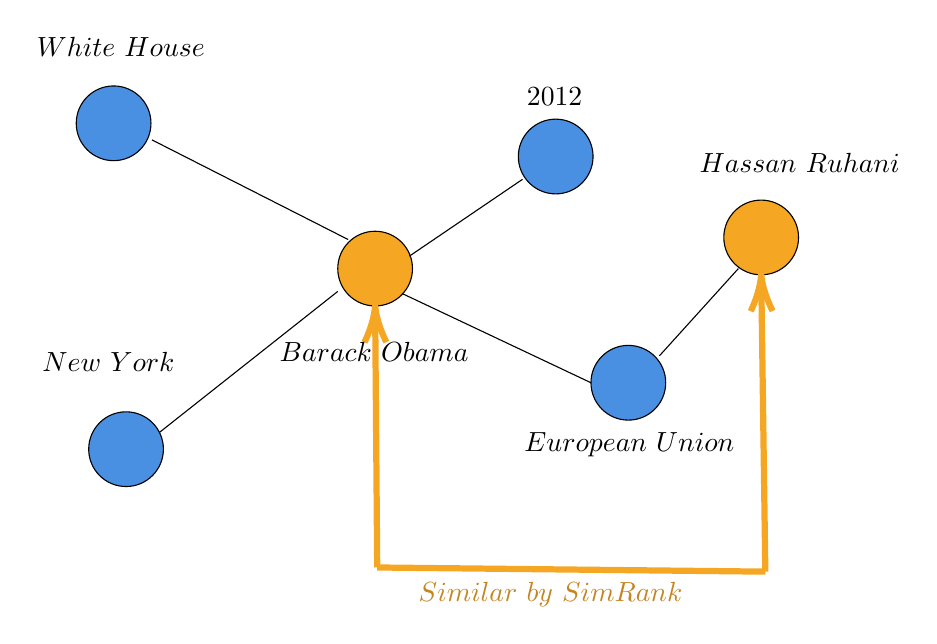
\begin{tikzpicture}[x=0.75pt,y=0.75pt,yscale=-1,xscale=1]
%uncomment if require: \path (0,407); %set diagram left start at 0, and has height of 407

%Shape: Circle [id:dp7237033228697587] 
\draw  [color={rgb, 255:red, 0; green, 0; blue, 0 }  ,draw opacity=1 ][fill={rgb, 255:red, 74; green, 144; blue, 226 }  ,fill opacity=1 ] (142.5,97) .. controls (142.5,87.06) and (150.56,79) .. (160.5,79) .. controls (170.44,79) and (178.5,87.06) .. (178.5,97) .. controls (178.5,106.94) and (170.44,115) .. (160.5,115) .. controls (150.56,115) and (142.5,106.94) .. (142.5,97) -- cycle ;
%Straight Lines [id:da7651994649420626] 
\draw    (179,105) -- (273.5,153) ;


%Shape: Circle [id:dp1628508691866306] 
\draw  [color={rgb, 255:red, 0; green, 0; blue, 0 }  ,draw opacity=1 ][fill={rgb, 255:red, 74; green, 144; blue, 226 }  ,fill opacity=1 ] (148.5,254) .. controls (148.5,244.06) and (156.56,236) .. (166.5,236) .. controls (176.44,236) and (184.5,244.06) .. (184.5,254) .. controls (184.5,263.94) and (176.44,272) .. (166.5,272) .. controls (156.56,272) and (148.5,263.94) .. (148.5,254) -- cycle ;
%Shape: Circle [id:dp6369036191517297] 
\draw  [color={rgb, 255:red, 0; green, 0; blue, 0 }  ,draw opacity=1 ][fill={rgb, 255:red, 245; green, 166; blue, 35 }  ,fill opacity=1 ] (268.5,167) .. controls (268.5,157.06) and (276.56,149) .. (286.5,149) .. controls (296.44,149) and (304.5,157.06) .. (304.5,167) .. controls (304.5,176.94) and (296.44,185) .. (286.5,185) .. controls (276.56,185) and (268.5,176.94) .. (268.5,167) -- cycle ;
%Shape: Circle [id:dp6138711151460285] 
\draw  [color={rgb, 255:red, 0; green, 0; blue, 0 }  ,draw opacity=1 ][fill={rgb, 255:red, 74; green, 144; blue, 226 }  ,fill opacity=1 ] (390.5,222) .. controls (390.5,212.06) and (398.56,204) .. (408.5,204) .. controls (418.44,204) and (426.5,212.06) .. (426.5,222) .. controls (426.5,231.94) and (418.44,240) .. (408.5,240) .. controls (398.56,240) and (390.5,231.94) .. (390.5,222) -- cycle ;
%Shape: Circle [id:dp15908024717263558] 
\draw  [color={rgb, 255:red, 0; green, 0; blue, 0 }  ,draw opacity=1 ][fill={rgb, 255:red, 74; green, 144; blue, 226 }  ,fill opacity=1 ] (355.5,113) .. controls (355.5,103.06) and (363.56,95) .. (373.5,95) .. controls (383.44,95) and (391.5,103.06) .. (391.5,113) .. controls (391.5,122.94) and (383.44,131) .. (373.5,131) .. controls (363.56,131) and (355.5,122.94) .. (355.5,113) -- cycle ;
%Straight Lines [id:da4548959711882159] 
\draw    (303,161) -- (357.5,124) ;


%Straight Lines [id:da6860631222603604] 
\draw    (299.5,179) -- (390.5,222) ;


%Straight Lines [id:da5778462671903315] 
\draw    (423.5,209) -- (461.5,167) ;


%Shape: Circle [id:dp9805133554604324] 
\draw  [color={rgb, 255:red, 0; green, 0; blue, 0 }  ,draw opacity=1 ][fill={rgb, 255:red, 245; green, 166; blue, 35 }  ,fill opacity=1 ] (454.5,152) .. controls (454.5,142.06) and (462.56,134) .. (472.5,134) .. controls (482.44,134) and (490.5,142.06) .. (490.5,152) .. controls (490.5,161.94) and (482.44,170) .. (472.5,170) .. controls (462.56,170) and (454.5,161.94) .. (454.5,152) -- cycle ;
%Straight Lines [id:da3078528737086299] 
\draw    (182.5,246) -- (268.5,178) ;


%Straight Lines [id:da6689641936732076] 
\draw [color={rgb, 255:red, 245; green, 166; blue, 35 }  ,draw opacity=1 ][line width=2.25]    (287.5,311) -- (286.53,189) ;
\draw [shift={(286.5,185)}, rotate = 449.55] [color={rgb, 255:red, 245; green, 166; blue, 35 }  ,draw opacity=1 ][line width=2.25]    (17.49,-5.26) .. controls (11.12,-2.23) and (5.29,-0.48) .. (0,0) .. controls (5.29,0.48) and (11.12,2.23) .. (17.49,5.26)   ;

%Straight Lines [id:da23704536821016675] 
\draw [color={rgb, 255:red, 245; green, 166; blue, 35 }  ,draw opacity=1 ][line width=2.25]    (474.5,313) -- (472.56,174) ;
\draw [shift={(472.5,170)}, rotate = 449.2] [color={rgb, 255:red, 245; green, 166; blue, 35 }  ,draw opacity=1 ][line width=2.25]    (17.49,-5.26) .. controls (11.12,-2.23) and (5.29,-0.48) .. (0,0) .. controls (5.29,0.48) and (11.12,2.23) .. (17.49,5.26)   ;

%Straight Lines [id:da7509045062366104] 
\draw [color={rgb, 255:red, 245; green, 166; blue, 35 }  ,draw opacity=1 ][line width=2.25]    (287.5,311) -- (474.5,313) ;



% Text Node
\draw (164,60) node   {$White\ House$};
% Text Node
\draw (286,207) node   {$Barack\ Obama$};
% Text Node
\draw (409,252) node   {$European\ Union$};
% Text Node
\draw (491,116) node   {$Hassan\ Ruhani$};
% Text Node
\draw (158,212) node   {$New\ York$};
% Text Node
\draw (373,84) node   {$2012$};
% Text Node
\draw (371,324) node [color={rgb, 255:red, 196; green, 133; blue, 33 }  ,opacity=1 ]  {$Similar\ by\ SimRank$};


\end{tikzpicture}


}
\caption{An example of SimRank similarity. In this graph, although the relationship between the president of Iran and the US is discovered by SimRank, the more important relationships, namely direct neighbours are disregarded. The similarity between \emph{``Barack Obama"} and the direct neighbours are zero.  }
\label{fig:simrank}
\end{figure}
\noindent
The VERSE model does not support the incorporation of the edge weights. From the three similarity measure that VERSE offers, we chose Adjacency Similarity to produce the entity embeddings. Our reason is two-folded: first, the PPR relates to the stationary distribution of a random walk with restart and we already represented the random walk-based models with DeepWalk. Second, SimRank is a measure of structural relatedness, between two nodes, based on the assumption that two nodes are
similar if they are connected to other similar nodes. Although words that happen often with the same words can themselves be considered similar, if we only look at nodes that have common neighbours we lose most of the adjacency relations in the graph. An example is illustrated in Figure~\ref{fig:simrank}. Since the SimRank of two nodes with no common neighbour, is zero, the direct neighbour are disregarded. However, SimRank tends to discover interesting relationship, such as the one shown in Figure~\ref{fig:simrank} and possibly if a new similarity measure is introduced that creates a trade-off between SimRank and Adjacency Similarity, the results might improve. For this study, however, we choose only Adjacency Similarity to learn the embeddings. Adjacency Similarity is based on the normalized adjacency matrix and captures the neighborhood relations. Moreover, it correlates with the first-order proximity in LINE and can be used as representative of first-order proximity. \\
The general pipeline for generation of entity-based embeddings is shown in Figure~\ref{fig:entity_emebddings_pipline}. Word and graph-based models the first steps of annotation, where the graph-based models have an additional step of co-occurrence graph extraction. Nodes of the graph are the named entities and terms in the text, thus, through embedding the nodes we achieve similar results. 
\begin{figure}
\centering 
\resizebox{0.97\textwidth}{0.32\textwidth}{      
\begin{tikzpicture}[x=0.75pt,y=0.75pt,yscale=-1,xscale=1]
%uncomment if require: \path (0,635); %set diagram left start at 0, and has height of 635

%Image [id:dp6574947802299504] 
\draw (75.75,317) node  {
\includegraphics[width=130.13pt,height=153pt]{images/document.png}};
%Image [id:dp6561738717090428] 
\draw (439,328.5) node  {
\includegraphics[width=138pt,height=158.25pt]{images/file.png}};
%Right Arrow [id:dp9146721412252041] 
\draw  [color={rgb, 255:red, 245; green, 166; blue, 35 }  ,draw opacity=1 ][fill={rgb, 255:red, 245; green, 166; blue, 35 }  ,fill opacity=0.47 ] (148,289.5) -- (273.1,289.5) -- (273.1,245) -- (356.5,334) -- (273.1,423) -- (273.1,378.5) -- (148,378.5) -- cycle ;
%Right Arrow [id:dp09556317236028589] 
\draw  [color={rgb, 255:red, 245; green, 166; blue, 35 }  ,draw opacity=1 ][fill={rgb, 255:red, 245; green, 166; blue, 35 }  ,fill opacity=0.47 ] (550.33,331.1) -- (650.69,390.66) -- (673.4,352.39) -- (694.88,468.64) -- (582.55,505.46) -- (605.26,467.19) -- (504.91,407.63) -- cycle ;
%Right Arrow [id:dp5897143294880893] 
\draw  [color={rgb, 255:red, 245; green, 166; blue, 35 }  ,draw opacity=1 ][fill={rgb, 255:red, 245; green, 166; blue, 35 }  ,fill opacity=0.47 ] (516.41,260.21) -- (624.6,216.45) -- (607.91,175.2) -- (713.41,228.54) -- (674.65,340.22) -- (657.97,298.96) -- (549.78,342.72) -- cycle ;
%Shape: Circle [id:dp3434778400848768] 
\draw  [fill={rgb, 255:red, 155; green, 155; blue, 155 }  ,fill opacity=1 ] (709,407) .. controls (709,398.72) and (715.72,392) .. (724,392) .. controls (732.28,392) and (739,398.72) .. (739,407) .. controls (739,415.28) and (732.28,422) .. (724,422) .. controls (715.72,422) and (709,415.28) .. (709,407) -- cycle ;
%Shape: Circle [id:dp1436491348522435] 
\draw  [color={rgb, 255:red, 74; green, 74; blue, 74 }  ,draw opacity=0.93 ][fill={rgb, 255:red, 155; green, 155; blue, 155 }  ,fill opacity=1 ] (797,410) .. controls (797,401.72) and (803.72,395) .. (812,395) .. controls (820.28,395) and (827,401.72) .. (827,410) .. controls (827,418.28) and (820.28,425) .. (812,425) .. controls (803.72,425) and (797,418.28) .. (797,410) -- cycle ;
%Shape: Circle [id:dp18392835474687086] 
\draw  [fill={rgb, 255:red, 120; green, 99; blue, 139 }  ,fill opacity=1 ] (684,491) .. controls (684,482.72) and (690.72,476) .. (699,476) .. controls (707.28,476) and (714,482.72) .. (714,491) .. controls (714,499.28) and (707.28,506) .. (699,506) .. controls (690.72,506) and (684,499.28) .. (684,491) -- cycle ;
%Shape: Circle [id:dp8124552092887645] 
\draw  [fill={rgb, 255:red, 191; green, 128; blue, 128 }  ,fill opacity=1 ] (812,476) .. controls (812,467.72) and (818.72,461) .. (827,461) .. controls (835.28,461) and (842,467.72) .. (842,476) .. controls (842,484.28) and (835.28,491) .. (827,491) .. controls (818.72,491) and (812,484.28) .. (812,476) -- cycle ;
%Shape: Circle [id:dp5058609984787195] 
\draw  [fill={rgb, 255:red, 74; green, 144; blue, 226 }  ,fill opacity=0.77 ] (749,576) .. controls (749,567.72) and (755.72,561) .. (764,561) .. controls (772.28,561) and (779,567.72) .. (779,576) .. controls (779,584.28) and (772.28,591) .. (764,591) .. controls (755.72,591) and (749,584.28) .. (749,576) -- cycle ;
%Shape: Circle [id:dp960474578620653] 
\draw  [fill={rgb, 255:red, 117; green, 167; blue, 159 }  ,fill opacity=1 ] (757,499) .. controls (757,490.72) and (763.72,484) .. (772,484) .. controls (780.28,484) and (787,490.72) .. (787,499) .. controls (787,507.28) and (780.28,514) .. (772,514) .. controls (763.72,514) and (757,507.28) .. (757,499) -- cycle ;
%Shape: Circle [id:dp7503802541142972] 
\draw  [fill={rgb, 255:red, 120; green, 99; blue, 139 }  ,fill opacity=1 ] (812,550) .. controls (812,541.72) and (818.72,535) .. (827,535) .. controls (835.28,535) and (842,541.72) .. (842,550) .. controls (842,558.28) and (835.28,565) .. (827,565) .. controls (818.72,565) and (812,558.28) .. (812,550) -- cycle ;
%Straight Lines [id:da9118524623122557] 
\draw    (724,422) -- (699,476) ;


%Straight Lines [id:da5895648837481868] 
\draw    (711,501) -- (757,499) ;


%Straight Lines [id:da3183776888797649] 
\draw    (800.5,421) -- (772,484) ;


%Straight Lines [id:da47281178753941844] 
\draw    (812,425) -- (819.5,461) ;


%Straight Lines [id:da31765662542163553] 
\draw    (699,506) -- (751.5,567) ;


%Straight Lines [id:da6125637100963139] 
\draw    (776.5,513) -- (812,550) ;


%Straight Lines [id:da5828194584982012] 
\draw    (776.5,513) -- (764,561) ;


%Straight Lines [id:da7333603221236795] 
\draw    (711.5,482) -- (797,410) ;


%Shape: Rectangle [id:dp6694535619063171] 
\draw  [color={rgb, 255:red, 255; green, 255; blue, 255 }  ,draw opacity=1 ][fill={rgb, 255:red, 74; green, 144; blue, 226 }  ,fill opacity=0.5 ] (766,179) -- (829,179) -- (829,206) -- (766,206) -- cycle ;
%Shape: Rectangle [id:dp813988003446805] 
\draw  [color={rgb, 255:red, 255; green, 255; blue, 255 }  ,draw opacity=1 ][fill={rgb, 255:red, 74; green, 144; blue, 226 }  ,fill opacity=0.5 ] (766,206) -- (829,206) -- (829,233) -- (766,233) -- cycle ;
%Right Arrow [id:dp5383294375674199] 
\draw  [color={rgb, 255:red, 245; green, 166; blue, 35 }  ,draw opacity=1 ][fill={rgb, 255:red, 245; green, 166; blue, 35 }  ,fill opacity=0.47 ] (848,447.75) -- (955.4,447.75) -- (955.4,408) -- (1027,487.5) -- (955.4,567) -- (955.4,527.25) -- (848,527.25) -- cycle ;
%Shape: Rectangle [id:dp8430332714333999] 
\draw  [color={rgb, 255:red, 255; green, 255; blue, 255 }  ,draw opacity=1 ][fill={rgb, 255:red, 74; green, 144; blue, 226 }  ,fill opacity=0.5 ] (767,234) -- (830,234) -- (830,261) -- (767,261) -- cycle ;
%Shape: Rectangle [id:dp7377615282291454] 
\draw  [color={rgb, 255:red, 255; green, 255; blue, 255 }  ,draw opacity=1 ][fill={rgb, 255:red, 74; green, 144; blue, 226 }  ,fill opacity=0.5 ] (767,261) -- (830,261) -- (830,288) -- (767,288) -- cycle ;
%Shape: Rectangle [id:dp3798861387841914] 
\draw  [color={rgb, 255:red, 255; green, 255; blue, 255 }  ,draw opacity=1 ][fill={rgb, 255:red, 74; green, 144; blue, 226 }  ,fill opacity=0.5 ] (829,154) -- (1047,154) -- (1047,179) -- (829,179) -- cycle ;
%Shape: Rectangle [id:dp5663017718009318] 
\draw  [color={rgb, 255:red, 255; green, 255; blue, 255 }  ,draw opacity=1 ][fill={rgb, 255:red, 74; green, 144; blue, 226 }  ,fill opacity=0.5 ] (1028,453) -- (1091,453) -- (1091,480) -- (1028,480) -- cycle ;
%Shape: Rectangle [id:dp728929889395908] 
\draw  [color={rgb, 255:red, 255; green, 255; blue, 255 }  ,draw opacity=1 ][fill={rgb, 255:red, 74; green, 144; blue, 226 }  ,fill opacity=0.5 ] (1028,480) -- (1091,480) -- (1091,507) -- (1028,507) -- cycle ;
%Shape: Rectangle [id:dp6263410500098714] 
\draw  [color={rgb, 255:red, 255; green, 255; blue, 255 }  ,draw opacity=1 ][fill={rgb, 255:red, 74; green, 144; blue, 226 }  ,fill opacity=0.5 ] (1029,508) -- (1092,508) -- (1092,535) -- (1029,535) -- cycle ;
%Shape: Rectangle [id:dp8754565727279509] 
\draw  [color={rgb, 255:red, 255; green, 255; blue, 255 }  ,draw opacity=1 ][fill={rgb, 255:red, 74; green, 144; blue, 226 }  ,fill opacity=0.5 ] (1029,535) -- (1092,535) -- (1092,562) -- (1029,562) -- cycle ;
%Shape: Rectangle [id:dp42451513571740374] 
\draw  [color={rgb, 255:red, 255; green, 255; blue, 255 }  ,draw opacity=1 ][fill={rgb, 255:red, 74; green, 144; blue, 226 }  ,fill opacity=0.5 ] (1091,428) -- (1309,428) -- (1309,453) -- (1091,453) -- cycle ;

% Text Node
\draw (74,318) node [scale=2.074,color={rgb, 255:red, 74; green, 74; blue, 74 }  ,opacity=1 ]  {$ \begin{array}{l}
Raw\ \\
Text
\end{array}$};
% Text Node
\draw (423,329) node [scale=2.074,color={rgb, 255:red, 74; green, 74; blue, 74 }  ,opacity=1 ]  {$ \begin{array}{l}
annotated\\
\ \ \ \ text
\end{array}$};
% Text Node
\draw (95,255) node   {$$};
% Text Node
\draw (246,332) node [scale=1.2]  {$ \begin{array}{l}
POS\ Tagging\\
Entity\ Recognition\\
Entity\ Disambiguation
\end{array}$};
% Text Node
\draw (610,421) node [scale=1.2,rotate=-31.79]  {$ \begin{array}{l}
Cooccurrence\ Graph\\
\ \ \ \ \ \ \ \ \ Extraction
\end{array}$};
% Text Node
\draw (605,265) node [scale=1.2,rotate=-334.44]  {$ \begin{array}{l}
Word\ Embedding\\
\ \ \ \ \ \ \ \ Models
\end{array}$};
% Text Node
\draw (798,194) node [scale=1.2]  {$T\_11$};
% Text Node
\draw (796,221) node [scale=1.2]  {$A\_15$};
% Text Node
\draw (924,490) node [scale=1.2]  {$ \begin{array}{l}
Node\ Embedding\\
\ \ \ \ \ \ \ \ \ Models
\end{array}$};
% Text Node
\draw (799,249) node [scale=1.2]  {$L\_9$};
% Text Node
\draw (798,276) node [scale=1.2]  {$O\_167$};
% Text Node
\draw (933,166) node [scale=1.2]  {$Dimensions$};
% Text Node
\draw (863,196) node   {$-0.1$};
% Text Node
\draw (915,196) node   {$-0.31$};
% Text Node
\draw (976,196) node   {$0.13$};
% Text Node
\draw (1024,195) node   {$...$};
% Text Node
\draw (861,222) node   {$0.1$};
% Text Node
\draw (912,222) node   {$1.23$};
% Text Node
\draw (975,222) node   {$8.7$};
% Text Node
\draw (1022,221) node   {$...$};
% Text Node
\draw (859,248) node   {$-0.41$};
% Text Node
\draw (911,248) node   {$-2.31$};
% Text Node
\draw (972,248) node   {$-0.6$};
% Text Node
\draw (1020,247) node   {$...$};
% Text Node
\draw (862,273) node   {$2.1$};
% Text Node
\draw (914,273) node   {$4.31$};
% Text Node
\draw (975,273) node   {$0.53$};
% Text Node
\draw (1023,271) node   {$...$};
% Text Node
\draw (795,298) node [rotate=-270]  {$...$};
% Text Node
\draw (1060,468) node [scale=1.2]  {$T\_11$};
% Text Node
\draw (1058,495) node [scale=1.2]  {$A\_15$};
% Text Node
\draw (1061,523) node [scale=1.2]  {$L\_9$};
% Text Node
\draw (1060,550) node [scale=1.2]  {$O\_167$};
% Text Node
\draw (1195,440) node [scale=1.2]  {$Dimensions$};
% Text Node
\draw (1125,470) node   {$-0.1$};
% Text Node
\draw (1177,470) node   {$-0.31$};
% Text Node
\draw (1238,470) node   {$0.13$};
% Text Node
\draw (1286,469) node   {$...$};
% Text Node
\draw (1123,496) node   {$0.1$};
% Text Node
\draw (1174,496) node   {$1.23$};
% Text Node
\draw (1237,496) node   {$8.7$};
% Text Node
\draw (1284,495) node   {$...$};
% Text Node
\draw (1121,522) node   {$-0.41$};
% Text Node
\draw (1173,522) node   {$-2.31$};
% Text Node
\draw (1234,522) node   {$-0.6$};
% Text Node
\draw (1282,521) node   {$...$};
% Text Node
\draw (1124,547) node   {$2.1$};
% Text Node
\draw (1176,547) node   {$4.31$};
% Text Node
\draw (1237,547) node   {$0.53$};
% Text Node
\draw (1285,545) node   {$...$};
% Text Node
\draw (1057,572) node [rotate=-270]  {$...$};


\end{tikzpicture}
		



}
\caption{Pipeline for generating entity-based embeddings. The first step is the annotation of the raw text with POS tagging, entity recognition, and disambiguation. Word embedding methods are applied to annotated corpus to create the textual models. A co-occurrence graph is extracted and nodes are embedded to achieve the graph-based models.   }
\label{fig:entity_emebddings_pipline}
\end{figure}
\section{Similarity Between Embeddings }\label{sec:similarity}
The dense word vector is learned to capture the semantics of the words and hence similar words are close in the induced space. \emph{cosine similarity} helps to capture this semantic closeness and is the most common similarity measure for the word vector. The cosine similarity is a measure that calculates the cosine of the angle between two vectors. This metric is a measurement of orientation and not magnitude and it is derived from the equation of a dot product between two vectors (Equation~\ref{eq:cosine}). The vectors are normalized by their length, which removes the influence of their magnitude on the similarity. The norm of the vector is somewhat related to the overall frequency of which words occur in the training corpus, but the direction is unaffected by this. So in order for a common word like \emph{``frog"} to still be similar to a less frequent word like \emph{``Anura"} (a type of frog), cosine distance which only looks at the direction works better than simple Euclidean distance. Moreover, cosine similarity is symmetric and changing the order of vectors in the dot product does not affect the final result.
\begin{equation}
\begin{split}
\overrightarrow { w_i } .\overrightarrow { w_j } =\parallel \overrightarrow { w_i } \parallel \parallel \overrightarrow { w_j } \parallel cos\theta 
\\
cos\theta =\frac { \overrightarrow { w_i } .\overrightarrow { w_j }  }{ \parallel \overrightarrow { w_i } \parallel \parallel \overrightarrow { w_j } \parallel  } 
\end{split}
\label{eq:cosine}
\end{equation}
\ornament
In this chapter,  two methods to extract entity and term embeddings from an annotated corpus were introduced. One method learns the embeddings directly from the text, while the other one generates a co-occurrence graph and embeds the nodes. In the next Chapter we attempt to create embeddings separable by entity type and in In Chapter~\ref{chap:eval}, we report the evaluation results for both entity based and facetted embeddings. We also show why the extraction of a co-occurrence graph is crucial for achieving better performance. 


   %%%%%%%%%%%%%%%%%%%%%%%%%%%%%%%%%%%%%%%%%%%%%%%%%%%%%%%%%%%%
\chapter{Faceted Embedding Model}\label{chap:faceted}
To further understand the effect of each entity type on the meaning of a word and as an effort to make the dimension of entity embeddings more interpretable, we experiment with creating embeddings with separable parts. By studying these models we gain some insights about the significance of each entity type for vector representations of words and explore if the embedding can be efficiently divided based on these types. In order to create these faceted models, we modify the well-established word embedding and graph-embedding techniques. In Section~\ref{sec:faceted_overview}, an overview of the objectives is given. In Section~\ref{sec:faceted_glove}, the first model based on the GloVe word embedding is proposed. For the faceted GloVe, we experiment with different cost functions, to obtain good performance. In Section~\ref{sec:faceted_word2vec}, a faceted model based on word2vec is introduced, which takes the edges of a co-occurrence graph as input. Since the graph-based embeddings performed the best for entity-based embeddings, we experiment with DeepWalk to generate similar embeddings for the faceted model in Section~\ref{sec:faceted_deepwalk}. For all models, the modifications to the original techniques and training procedures are discussed. 
 %%%%%%%%%%%%%%%%%%%%%%%%%%%%%%%%%%%%%%%%%%%%%%%%%%%%%%%%%%%%
\section{Overview and Objectives}\label{sec:faceted_overview}
Word embedding are in general very ambiguous, it is unknown what the value in the vector representation indicate, if each value corresponds to a distinct attribute of the word or shows the to what degree each word belongs to a certain group. We introduce the faceted embedding models to address this problems, where we divide the word embedding into components that show a pre-defined attribute of each word, namely its relation to entities with specific type. 
\begin{figure}
\centering 
\resizebox{0.97\textwidth}{0.16\textwidth}{      
\begin{tikzpicture}[x=0.75pt,y=0.75pt,yscale=-1,xscale=1]
%uncomment if require: \path (0,635); %set diagram left start at 0, and has height of 635

%Image [id:dp7437455745259745] 
\draw (74.75,328) node  {
\includegraphics[width=130.13pt,height=153pt]{images/document.png}};
%Image [id:dp9326691131220199] 
\draw (439,328.5) node  {
\includegraphics[width=138pt,height=158.25pt]{images/file.png}};
%Right Arrow [id:dp8162584732827316] 
\draw  [color={rgb, 255:red, 245; green, 166; blue, 35 }  ,draw opacity=1 ][fill={rgb, 255:red, 245; green, 166; blue, 35 }  ,fill opacity=0.47 ] (148,289.5) -- (273.1,289.5) -- (273.1,245) -- (356.5,334) -- (273.1,423) -- (273.1,378.5) -- (148,378.5) -- cycle ;
%Right Arrow [id:dp04654387721869724] 
\draw  [color={rgb, 255:red, 245; green, 166; blue, 35 }  ,draw opacity=1 ][fill={rgb, 255:red, 245; green, 166; blue, 35 }  ,fill opacity=0.47 ] (526.95,295.43) -- (637.47,293.41) -- (636.66,248.92) -- (711.97,336.55) -- (639.92,426.89) -- (639.1,382.39) -- (528.58,384.42) -- cycle ;
%Shape: Circle [id:dp0628135614312153] 
\draw  [fill={rgb, 255:red, 155; green, 155; blue, 155 }  ,fill opacity=1 ] (743,251) .. controls (743,242.72) and (749.72,236) .. (758,236) .. controls (766.28,236) and (773,242.72) .. (773,251) .. controls (773,259.28) and (766.28,266) .. (758,266) .. controls (749.72,266) and (743,259.28) .. (743,251) -- cycle ;
%Shape: Circle [id:dp4682523800222689] 
\draw  [color={rgb, 255:red, 74; green, 74; blue, 74 }  ,draw opacity=0.93 ][fill={rgb, 255:red, 155; green, 155; blue, 155 }  ,fill opacity=1 ] (831,254) .. controls (831,245.72) and (837.72,239) .. (846,239) .. controls (854.28,239) and (861,245.72) .. (861,254) .. controls (861,262.28) and (854.28,269) .. (846,269) .. controls (837.72,269) and (831,262.28) .. (831,254) -- cycle ;
%Shape: Circle [id:dp16445174812495322] 
\draw  [fill={rgb, 255:red, 120; green, 99; blue, 139 }  ,fill opacity=1 ] (714,340) .. controls (714,331.72) and (720.72,325) .. (729,325) .. controls (737.28,325) and (744,331.72) .. (744,340) .. controls (744,348.28) and (737.28,355) .. (729,355) .. controls (720.72,355) and (714,348.28) .. (714,340) -- cycle ;
%Shape: Circle [id:dp7077138452602891] 
\draw  [fill={rgb, 255:red, 191; green, 128; blue, 128 }  ,fill opacity=1 ] (846,320) .. controls (846,311.72) and (852.72,305) .. (861,305) .. controls (869.28,305) and (876,311.72) .. (876,320) .. controls (876,328.28) and (869.28,335) .. (861,335) .. controls (852.72,335) and (846,328.28) .. (846,320) -- cycle ;
%Shape: Circle [id:dp026745379039323947] 
\draw  [fill={rgb, 255:red, 74; green, 144; blue, 226 }  ,fill opacity=0.77 ] (783,420) .. controls (783,411.72) and (789.72,405) .. (798,405) .. controls (806.28,405) and (813,411.72) .. (813,420) .. controls (813,428.28) and (806.28,435) .. (798,435) .. controls (789.72,435) and (783,428.28) .. (783,420) -- cycle ;
%Shape: Circle [id:dp0822183171369899] 
\draw  [fill={rgb, 255:red, 117; green, 167; blue, 159 }  ,fill opacity=1 ] (791,343) .. controls (791,334.72) and (797.72,328) .. (806,328) .. controls (814.28,328) and (821,334.72) .. (821,343) .. controls (821,351.28) and (814.28,358) .. (806,358) .. controls (797.72,358) and (791,351.28) .. (791,343) -- cycle ;
%Shape: Circle [id:dp8571642965600172] 
\draw  [fill={rgb, 255:red, 120; green, 99; blue, 139 }  ,fill opacity=1 ] (846,394) .. controls (846,385.72) and (852.72,379) .. (861,379) .. controls (869.28,379) and (876,385.72) .. (876,394) .. controls (876,402.28) and (869.28,409) .. (861,409) .. controls (852.72,409) and (846,402.28) .. (846,394) -- cycle ;
%Straight Lines [id:da9213704364324085] 
\draw    (758,266) -- (729,325) ;


%Straight Lines [id:da7126571751614004] 
\draw    (745,345) -- (791,343) ;


%Straight Lines [id:da47175239635743016] 
\draw    (834.5,265) -- (806,328) ;


%Straight Lines [id:da5974054442400747] 
\draw    (846,269) -- (853.5,305) ;


%Straight Lines [id:da7185517043699976] 
\draw    (733,350) -- (785.5,411) ;


%Straight Lines [id:da648492395956862] 
\draw    (810.5,357) -- (846,394) ;


%Straight Lines [id:da8600323300544932] 
\draw    (810.5,357) -- (798,405) ;


%Straight Lines [id:da9764033267651315] 
\draw    (744,328) -- (831,254) ;


%Right Arrow [id:dp1882901124628904] 
\draw  [color={rgb, 255:red, 245; green, 166; blue, 35 }  ,draw opacity=1 ][fill={rgb, 255:red, 245; green, 166; blue, 35 }  ,fill opacity=0.47 ] (879,298.5) -- (986.4,298.5) -- (986.4,252) -- (1058,345) -- (986.4,438) -- (986.4,391.5) -- (879,391.5) -- cycle ;
%Shape: Rectangle [id:dp22528256222017617] 
\draw  [color={rgb, 255:red, 255; green, 255; blue, 255 }  ,draw opacity=1 ][fill={rgb, 255:red, 74; green, 144; blue, 226 }  ,fill opacity=0.5 ] (1058,288) -- (1121,288) -- (1121,315) -- (1058,315) -- cycle ;
%Shape: Rectangle [id:dp7626014323484545] 
\draw  [color={rgb, 255:red, 255; green, 255; blue, 255 }  ,draw opacity=1 ][fill={rgb, 255:red, 74; green, 144; blue, 226 }  ,fill opacity=0.5 ] (1058,315) -- (1121,315) -- (1121,342) -- (1058,342) -- cycle ;
%Shape: Rectangle [id:dp2994514356517668] 
\draw  [color={rgb, 255:red, 255; green, 255; blue, 255 }  ,draw opacity=1 ][fill={rgb, 255:red, 74; green, 144; blue, 226 }  ,fill opacity=0.5 ] (1059,343) -- (1122,343) -- (1122,370) -- (1059,370) -- cycle ;
%Shape: Rectangle [id:dp22924765237906586] 
\draw  [color={rgb, 255:red, 255; green, 255; blue, 255 }  ,draw opacity=1 ][fill={rgb, 255:red, 74; green, 144; blue, 226 }  ,fill opacity=0.5 ] (1059,370) -- (1122,370) -- (1122,397) -- (1059,397) -- cycle ;
%Shape: Rectangle [id:dp35487479154274304] 
\draw  [color={rgb, 255:red, 255; green, 255; blue, 255 }  ,draw opacity=1 ][fill={rgb, 255:red, 74; green, 144; blue, 226 }  ,fill opacity=0.5 ] (1121,263) -- (1339,263) -- (1339,288) -- (1121,288) -- cycle ;

% Text Node
\draw (74,320) node [scale=2.074,color={rgb, 255:red, 74; green, 74; blue, 74 }  ,opacity=1 ]  {$ \begin{array}{l}
Raw\ \\
Text
\end{array}$};
% Text Node
\draw (423,329) node [scale=2.074,color={rgb, 255:red, 74; green, 74; blue, 74 }  ,opacity=1 ]  {$ \begin{array}{l}
annotated\\
\ \ \ \ text
\end{array}$};
% Text Node
\draw (95,255) node   {$$};
% Text Node
\draw (243,334) node [scale=1.2]  {$ \begin{array}{l}
POS\ Tagging\\
Entity\ Recognition\\
Entity\ Disambiguation
\end{array}$};
% Text Node
\draw (613.98,340.5) node [scale=1.2,rotate=-0.05]  {$ \begin{array}{l}
Cooccurrence\ Graph\\
\ \ \ \ \ \ \ \ \ Extraction
\end{array}$};
% Text Node
\draw (957,356) node [scale=1.2]  {$ \begin{array}{l}
Node\ Embedding\\
\ \ \ \ \ \ \ \ \ \ \ \ \ \ or\ \\
Word\ Embedding\\
\ \ \ \ \ 
\end{array}$};
% Text Node
\draw (1090,303) node [scale=1.2]  {$T\_11$};
% Text Node
\draw (1088,330) node [scale=1.2]  {$A\_15$};
% Text Node
\draw (1091,358) node [scale=1.2]  {$L\_9$};
% Text Node
\draw (1090,385) node [scale=1.2]  {$O\_167$};
% Text Node
\draw (1225,275) node [scale=1.2]  {$Dimensions$};
% Text Node
\draw (1155,305) node   {$-0.1$};
% Text Node
\draw (1207,305) node   {$-0.31$};
% Text Node
\draw (1268,305) node   {$0.13$};
% Text Node
\draw (1316,304) node   {$...$};
% Text Node
\draw (1153,331) node   {$0.1$};
% Text Node
\draw (1204,331) node   {$1.23$};
% Text Node
\draw (1267,331) node   {$8.7$};
% Text Node
\draw (1314,330) node   {$...$};
% Text Node
\draw (1151,357) node   {$-0.41$};
% Text Node
\draw (1203,357) node   {$-2.31$};
% Text Node
\draw (1264,357) node   {$-0.6$};
% Text Node
\draw (1312,356) node   {$...$};
% Text Node
\draw (1154,382) node   {$2.1$};
% Text Node
\draw (1206,382) node   {$4.31$};
% Text Node
\draw (1267,382) node   {$0.53$};
% Text Node
\draw (1315,380) node   {$...$};


\end{tikzpicture}

}
\caption{Pipeline for generating faceted embeddings. The first step is the annotation of the raw text with POS tagging, entity recognition, and disambiguation. A co-occurrence graph is extracted, which is used as input for node embedding or variation of word embedding methods.   }
\label{fig:facetted_pipeline}
\end{figure}
Since we are looking at entity-based relations, the corpus should be annotated with named entities. A general pipeline of the approach is shown in Figure~\ref{fig:facetted_pipeline}, where the entity recognition and disambiguation is applied to the input text which is used to extract a co-occurrence graph. The graph representation of the corpus is then used by graph-based embeddings or variations of common word embedding techniques to generate a typed embedding, in which the instead of capturing the semantic of a word in relation to the entire vocabulary (as normal word embeddings do), we capture the semantic in relation to entities of a specific type. This process is repeated for all the entity type available for the model, which results into multiple embedding, each specific to a type. These embeddings can be concatenated to generate a final embedding or used separately based on the use-case scenario. \\
Ideally, a faceted model is able to capture the surrounding relation for each type separately in different components of the vector, where the relation to entities that co-occur with a word would be captured by the corresponding component. An illustration of a faceted embedding for the entity \emph{``Donald Trump''} is shown in Figure~\ref{fig:faceted_emb}. The center word is the entity \emph{``Donald Trump''} marked in red and each type is annotated with the different color in the text. Any word that is not an entity or a date is considered a term. Each component is responsible for mapping the entity \emph{``Donald Trump''} in the neighbourhood of entities of a specific type that co-occur with it. \\
\begin{figure}
\centering 
\resizebox{0.97\textwidth}{0.3\textwidth}{      
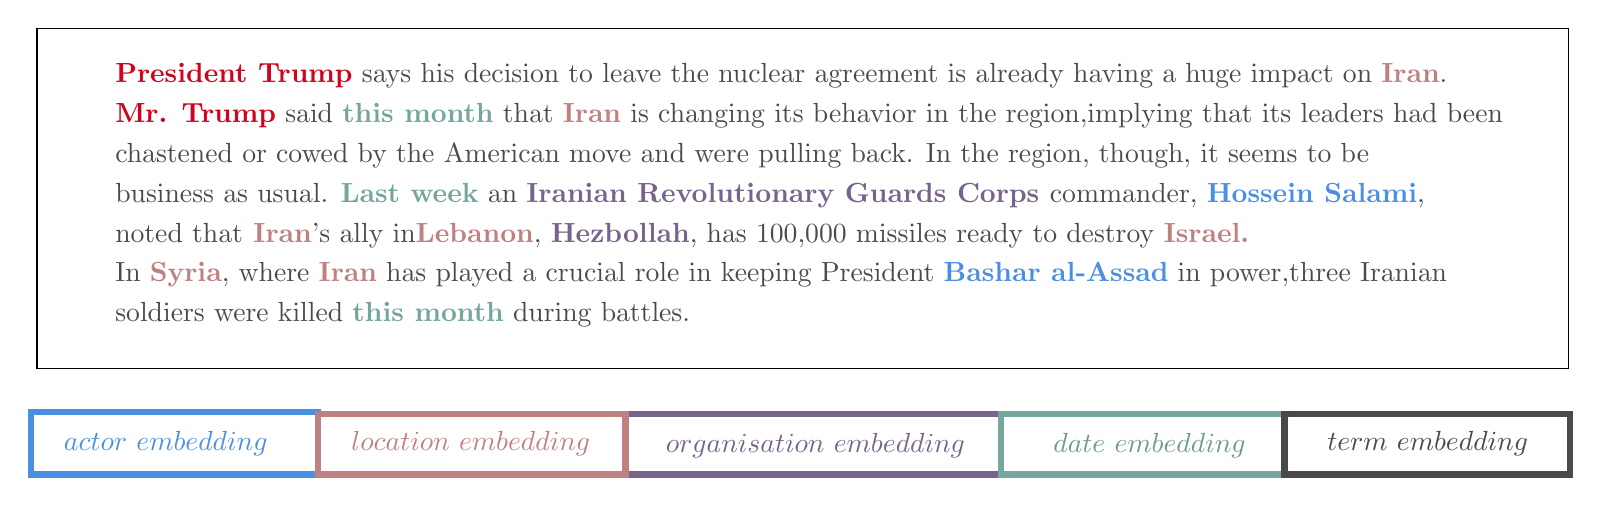
\begin{tikzpicture}[x=0.75pt,y=0.75pt,yscale=-1,xscale=1]
%uncomment if require: \path (0,300); %set diagram left start at 0, and has height of 300

\draw  [color={rgb, 255:red, 74; green, 144; blue, 226 }  ,draw opacity=1 ][line width=2.25]   (13, 207) rectangle (151.5, 237)   ;
\draw  [color={rgb, 255:red, 120; green, 99; blue, 139 }  ,draw opacity=1 ][line width=2.25]   (299.5, 208) rectangle (480.5, 237)   ;
\draw  [color={rgb, 255:red, 191; green, 128; blue, 128 }  ,draw opacity=1 ][line width=2.25]   (151.5, 208) rectangle (299.5, 237)   ;
\draw  [color={rgb, 255:red, 117; green, 167; blue, 159 }  ,draw opacity=1 ][line width=2.25]   (480.5, 208) rectangle (617, 237)   ;
\draw  [color={rgb, 255:red, 74; green, 74; blue, 74 }  ,draw opacity=1 ][line width=2.25]   (617, 208) rectangle (754.5, 237)   ;
\draw    (16, 22) rectangle (754, 186)   ;

\draw (78,222) node [color={rgb, 255:red, 74; green, 144; blue, 226 }  ,opacity=1 ]  {$actor\ embedding$};
\draw (225,222) node [color={rgb, 255:red, 191; green, 128; blue, 128 }  ,opacity=1 ]  {$location\ embedding$};
\draw (391,223) node [color={rgb, 255:red, 120; green, 99; blue, 139 }  ,opacity=1 ]  {$organisation\ embedding$};
\draw (552,223) node [color={rgb, 255:red, 108; green, 153; blue, 146 }  ,opacity=1 ]  {$date\ embedding$};
\draw (686,222) node [color={rgb, 255:red, 74; green, 74; blue, 74 }  ,opacity=1 ]  {$term\ embedding$};
\draw (388,130) node [scale=1,color={rgb, 255:red, 74; green, 74; blue, 74 }  ,opacity=1 ] [align=left] {\textcolor[rgb]{0.82,0.01,0.11}{\textbf{President Trump}} says his decision to leave the nuclear agreement is already having a huge impact on \textcolor[rgb]{0.75,0.5,0.5}{\textbf{Iran}}.\\\textcolor[rgb]{0.82,0.01,0.11}{\textbf{Mr. Trump}} said \textcolor[rgb]{0.46,0.65,0.62}{\textbf{this month}} that \textcolor[rgb]{0.75,0.5,0.5}{\textbf{Iran}} is changing its behavior in the region,implying that its leaders had been \\\textcolor[rgb]{0.29,0.29,0.29}{chastened or cowed by the American move and were pulling back. In the region, though, it seems to be}\\business as usual. \textcolor[rgb]{0.46,0.65,0.62}{\textbf{Last week}} an \textbf{\textcolor[rgb]{0.47,0.39,0.55}{Iranian Revolutionary Guards Corps} }commander, \textcolor[rgb]{0.29,0.56,0.89}{\textbf{Hossein Salami}}, \\noted that\textbf{ \textcolor[rgb]{0.75,0.5,0.5}{Iran}}’s ally in\textcolor[rgb]{0.75,0.5,0.5}{ \textbf{Lebanon}}, \textcolor[rgb]{0.47,0.39,0.55}{\textbf{Hezbollah}}, has 100,000 missiles ready to destroy \textbf{\textcolor[rgb]{0.75,0.5,0.5}{Israel.}} \\In \textcolor[rgb]{0.75,0.5,0.5}{\textbf{Syria}}, where \textcolor[rgb]{0.75,0.5,0.5}{\textbf{Iran}} has played a crucial role in keeping President \textcolor[rgb]{0.29,0.56,0.89}{\textbf{Bashar al-Assad}} in power,three Iranian \\soldiers were killed \textcolor[rgb]{0.46,0.65,0.62}{\textbf{this month}} during battles.\\\\\\};


\end{tikzpicture}

}
\caption{Faceted embedding of the entity \emph{``Donald Trump''} for a short paragraph. Each part of the embedding corresponds to the relation of the center word to that specific type. Each entity type is illustrated with matching color in text and embedding. }
\label{fig:faceted_emb}
\end{figure} 
Some of the potential advantages and motivation for analysing each part separately are as follows: 
\begin{compactitem}
\item \emph{Interpretability of relations:} Since each part of the embedding vector encodes relations to one of the entity types, e.g., the actors part only encodes the actors in the context of a word. Through this separate components, the relations between two word or entities become more interpretable. Any similarity measure to compare two word vectors can be applied to each component separately. Thus, the similarity of the words can be broken down into their different attributes. If two entities are closer in location space and farther in actors space, it is possible that they are situated close locally, but are not related to the same people. \\

\item \emph{Change in meaning:} Exploring and visualizing different components of an embedding over time gives us insights into how that entity has evolved overtime, with respect to that component. When applied to a corpus with a temporal aspect, like news articles, faceted models can illustrate how a word changes its meaning in relation to different types. For example, \emph{``Donald Trump''} is mentioned frequently in location context with \emph{``Iran''} during the discussion for the nuclear deal, but some time after the abandonment of the deal the topic fades away and \emph{``Donald Trump''}  is mentioned more often with relation to other countries. This information can be extracted from the location subspace of the word embedding. Consequently, the values for the location part of the embedding will bring the word vector closer to any other entity that is also frequently mentioned with Iran deal during the nuclear discussions like \emph{``Khamenei''} (Iran's supreme leader). Even if \emph{``Khamenei''} is not directly mentioned with \emph{``Donald Trump''}, they are mentioned in the same context location-wise, and, therefore, are mapped to points close to each other in the location domain. If embeddings are reconstructed for a time span after the nuclear abandonment, the two mentioned entities should become less similar in location aspect. Although the same experiment can be done on normal embeddings, where all the words are treated equally, the distinguishable components give us additional insights as to what aspect has invoked the change.\\

\item \emph{Interpretability of evaluation tasks:} Separable parts also plays a role in interpretability of evaluation tasks. We experiment with using only a specific component in our evaluations in Chapter~\ref{chap:eval} to find out which type of entity surrounding a word is more influential for a certain task.\\

\item \emph{Flexible neighbourhood search:} With faceted models, the search for a similar word or entity becomes more flexible. Same as the embedding space, the search space can be divided into various types, where one can look for neighbours in a specific context. The type-specific information can be used in the search, where one can query for entities that are closer to a certain word in the temporal or location aspect. For example, \emph{``Washington''} as a political person should appear more often with the same actors and has a different actor dimension than \emph{``Washington DC''} as a location. The standard embedding treats all the word equally and therefore cannot reflect this type of similarity. Since the dimensions are independent and can be combined in an arbitrary way, a combination of different dimensions can tailor the search results further and create a type-specific search. 
\end{compactitem}
To achieve this type of embeddings, we define faceted embeddings as word embeddings, where each dimension represents the relation of the embedded word to a specific type of entities surrounding it. Which types are considered during training is arbitrary, but for the purpose of this work, we choose to contain actors, locations, organisations, dates, and terms, since these types are available by the LOAD model. An example of such an embedding vector ($w$) for a corpus containing types of actor (ACT), location (LOC), organisation (ORG), date (DAT) and term (TER) is shown below: \\
\mathleft
\begin{equation}
w=\left[ \underbrace { \begin{matrix}{ a }_{ 1,1 } ... { a }_{ 1,M } \end{matrix} } |\underbrace { \begin{matrix}{ a }_{ 1,M+1 } ... { a }_{ 1,2M } \end{matrix} } |\underbrace { \begin{matrix}{ a }_{ 1,2M+1 } ... { a }_{ 1,3M } \end{matrix} } |\underbrace { \begin{matrix}{ a }_{ 1,3M+1 } ... { a }_{ 1,4M } \end{matrix} } |\underbrace { \begin{matrix}{ a }_{ 14M+1 } ... { a }_{ 1,5M } \end{matrix} }  \right] 
\label{eq:concat_vec}
\end{equation}
$$ \quad  \mathrm{ACT} \quad  \qquad  \mathrm{LOC}\qquad \qquad \mathrm{ORG}\qquad \quad \qquad \mathrm{DAT}\qquad \quad  \qquad  \mathrm{TER}\qquad \qquad$$
\mathcenter
Provided that the most common dimension for word embeddings are between $100$ to $300$, to maintain the same order of dimension in faceted embeddings all the different parts have the same dimension but in a lower magnitude ($20$ to $50$). These small embeddings are concatenated to create the final embedding. Each part is independent of the rest and is usually trained separately.
With these independent components, the embeddings stand to be more interpretable. Although a model that divides the embedding space into entity types has not been studied, some work has been done to make the vector representations more interpretable. In the work of Frauqui et al. transformation of word vectors into sparse (and optionally binary) vectors is proposed~\brackettext{\cite{DBLP:journals/corr/FaruquiTYDS15}}. Each vector is projected into an over-complete binary vector, where each dimension represents a feature similar to ones used in traditional NLP systems but found automatically during training. However, since their dimensions are binary valued, there is no notion of the extent to which a word participates in a particular dimension. Later, a model based on rotating the word vectors was introduced in order to improve the interpretability.~\brackettext{\cite{DBLP:conf/emnlp/ParkBO17}}. Recently, a neural network-based approach to the problem was introduced by using sparse auto-encoders~\brackettext{\cite{DBLP:conf/aaai/SubramanianPJBH18}}. Although these works shine some light on the potential meaning of each dimension, they focus purely on terms. whereas, we generate embeddings that each part reflects the word related to entities of a certain type and takes more than terms into account. As explained in Chapter~\ref{chap:background}, the aim of the word embedding is to reduce the high dimensional space of text and embed words into a meaningful space, where words with similar meaning are mapped to points close to each other. In the case of faceted embedding, it is as if we are dividing the textual space into all possible entity types, where each subspace contains only entities of a specific type. To put it differently, the space of all words $V$ is represented as $V=A\bigcup  L\bigcup  O\bigcup  D\bigcup \overline {N} $, where $A$,$L$,$O$,$D$ are the sets of all actors, locations, organisations and, dates, respectively and $ T=\overline{N}$ denotes all the words which are not a named entity. The goal is then to map each word into all the subspaces, where words that co-occur with the same entities of a specific type are mapped closer together. Since all the subspaces are independent of each other (e.g., the space of all actors does not have any of the location entities inside it), each embedding learned on the different subspace is also independent. Hence, it is perfectly reasonable that two words are close in one subspace and far in another. \\
In the remainder of this chapter, we aim to introduce faceted models as a general framework for learning embeddings with known types and separable dimensions. To create such embeddings we propose three approaches, two of which are based on word embedding models and one use the graph embedding techniques: 
\begin{compactenum}
\item Modifying the cost function of the GloVe model to train a separate embedding for each entity type on an annotated corpus. Although the original GloVe uses the word co-occurrence matrix as input, we transform the model to use the adjacency matrix of a co-occurrence graph. 
\item Using a variation of the word2vec model, which supports an arbitrary definition of context for each word to train an embedding for each entity type. This model is also trained on a corpus annotated with named entities.
\item Extracting a co-occurrence graph from the annotated text and modifying the graph embedding model to generate embeddings based on neighbours of a specific type. 
\end{compactenum}
 %%%%%%%%%%%%%%%%%%%%%%%%%%%%%%%%%%%%%%%%%%%%%%%%%%%%%%%%%%%%
\section{Faceted GloVe}\label{sec:faceted_glove}
In the previous chapter, we indicated that the LOAD edge weight captures the corpus relations similar to the co-occurrence matrix and that meaning components can be extracted from them. In this chapter, we use this knowledge to create faceted embeddings from the weighted adjacency matrix of the LOAD graph. In the first part, the construction of a weighted adjacency matrix is illustrated followed by the model definition. We denote the faceted GloVe model by $f$GLV, where \emph{``f''} indicates the faceted model. The proposed model contains two type of cost functions, that are discussed separately in Section~\ref{sec:normal_cost} and~\ref{sec:unified_cost}. \\
The complete training task can be formulated in four steps: 
 \begin{enumerate}        
 \item Extraction of co-occurrence matrices for different types, explained in Section~\ref{sec:adj_matrix}. 
 \item For each type, a GloVe based embedding is learned using either a separate or unified cost function, discussed separately in Section~\ref{sec:normal_cost} and~\ref{sec:unified_cost}. 
 \item The context embedding is kept and the focal embedding is either disregarded to added with focal addition, discussed in Section~\ref{sec:faceted_embeddings}.
 \item The results of the third step are different embeddings for each type, which can be concatenated to generate the final faceted embedding. 
 \end{enumerate}
 %%%%%%%%%%%%%%%%%%%%%%%%%%%%%%%%%%%%%%%%%%%%%%%%%%%%%%%%%%%%
\subsection{Weighted adjacency matrix}\label{sec:adj_matrix}
To learn the embeddings, a weighted adjacency matrix for each type of entity and term is needed (ACT, LOC, TER, ORG, DAT). The matrices are constructed based on the weighted edge list of the co-occurrence graph, where the weights can be co-occurrence counts (identical to the GloVe model) or, any other distance measure defined by the graph. For example, the weighted adjacency matrix for actors contains the edges that have an actor as start nodes and any other type as the end node. Since in this thesis we use undirected co-occurrence graphs, the same edge exists in the opposite direction. For instance, an edge between an actor and a term is repeated twice and will be used once to create the actor matrix and once to create the term matrix. More formally, the matrices can be constructed as shown in Figure~\ref{fig:co-matrix}, where the entries of the matrices are the edge weights between two words.  
\begin{figure}
%\[\mathrm{ACT}=
%\begin{blockarray}{cccccccc}
% &\mathrm{TER}_1  & \color{myblue}{ \mathrm{ORG}_1 } &  \mathrm{TER}_2  & \mathrm{ACT}_1 & \mathrm{DAT}_1 & \mathrm{LOC}_1 & ... \\
%\begin{block}{c(ccccccc)}
%  \mathrm{ACT}_1 &m_{00} & \color{myblue}{ m_{01}}  &  m_{02} & m_{03} & m_{04} &m_{00}& ... \\
%  \mathrm{ACT}_2 & m_{10} & \color{myblue}{ m_{11} } &  m_{12} & m_{13} & m_{14} &m_{15}& ... \\
%  \mathrm{ACT}_3 & m_{20} &  \color{myblue}{m_{21} } &  m_{22} & m_{23} & m_{24} &m_{25}& ... \\
%  .. & ... &  \color{myblue}{...}  &  ... & ... & ... &...& ... \\
%\end{block}
%\end{blockarray}
% \]
%\[\mathrm{ORG}=
%\begin{blockarray}{cccccccc}
% &\mathrm{TER}_1  & \color{myblue}{ \mathrm{ORG}_1} &  \mathrm{TER}_2  & \mathrm{ACT}_1 & \mathrm{DAT}_1 & \mathrm{LOC}_1 & ... \\
%\begin{block}{c(ccccccc)}
%  \mathrm{ORG}_1 &m_{00} & \color{myblue}{ m_{01}}  &  m_{02} & m_{03} & m_{04} &m_{00}& ... \\
%  \mathrm{ORG}_2 & m_{10} & \color{myblue}{ m_{11} } &  m_{12} & m_{13} & m_{14} &m_{15}& ... \\
%  \mathrm{ORG} _3& m_{20} &  \color{myblue}{m_{21} } &  m_{22} & m_{23} & m_{24} &m_{25}& ... \\
%  .. & ... &  \color{myblue}{...}  &  ... & ... & ... &...& ... \\
%\end{block}
%\end{blockarray}
% \]
% \[\mathrm{DAT}=
%\begin{blockarray}{cccccccc}
% &TER1  & \color{myblue}{ \mathrm{ORG}_1} &  \mathrm{TER}_2  & \mathrm{ACT}_1 & \mathrm{DAT}_1 & \mathrm{LOC}_1 & ... \\
%\begin{block}{c(ccccccc)}
%  \mathrm{DAT}_1 &m_{00} & \color{myblue}{ m_{01}}  &  m_{02} & m_{03} & m_{04} &m_{00}& ... \\
%  \mathrm{DAT}_2 & m_{10} & \color{myblue}{ m_{11} } &  m_{12} & m_{13} & m_{14} &m_{15}& ... \\
%  \mathrm{DAT}_3 & m_{20} &  \color{myblue}{m_{21} } &  m_{22} & m_{23} & m_{24} &m_{25}& ... \\
%  .. & ... &  \color{myblue}{...}  &  ... & ... & ... &...& ... \\
%\end{block}
%\end{blockarray}
% \]
\centering 
\resizebox{0.97\textwidth}{0.26\textwidth}{      
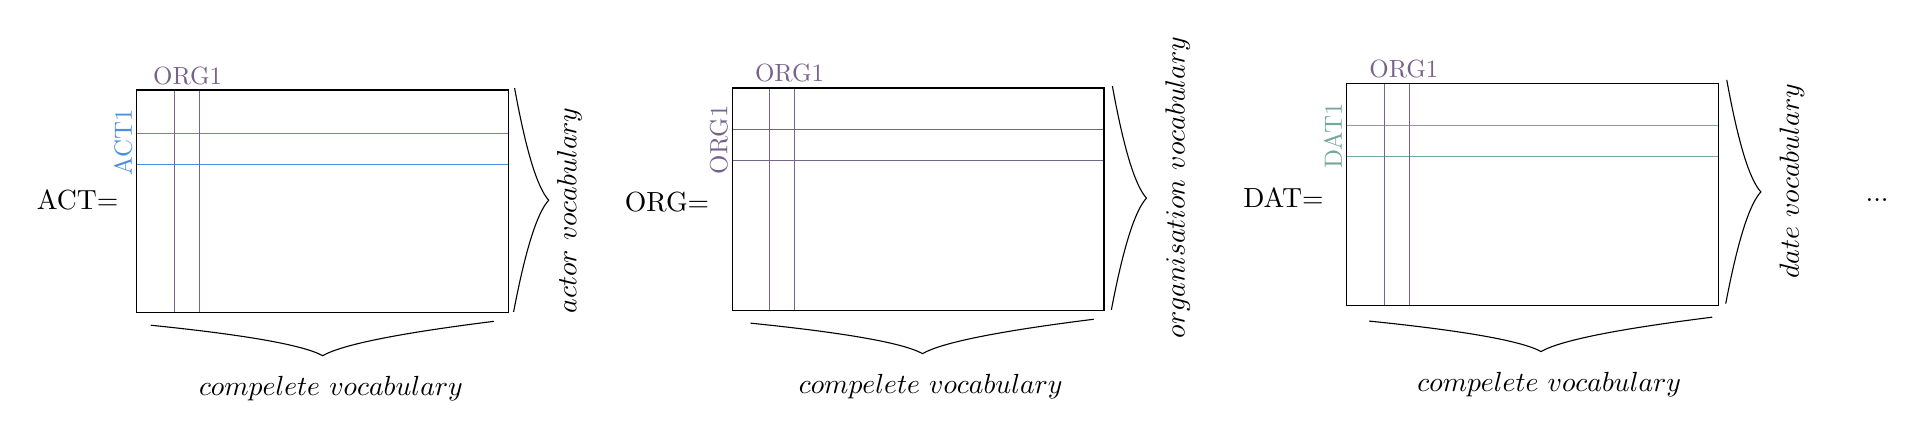
\begin{tikzpicture}[x=0.75pt,y=0.75pt,yscale=-1,xscale=1]
%uncomment if require: \path (0,370); %set diagram left start at 0, and has height of 370

%Shape: Rectangle [id:dp688565454623014] 
\draw  [color={rgb, 255:red, 74; green, 144; blue, 226 }  ,draw opacity=1 ] (55.5,122) -- (234.5,122) -- (234.5,137) -- (55.5,137) -- cycle ;
\draw   (227.55,212.43) .. controls (181.69,218.16) and (154.2,223.68) .. (145.07,228.99) .. controls (135.83,223.89) and (108.22,218.99) .. (62.24,214.31) ;
\draw   (237.54,100.09) .. controls (242.97,130.06) and (248.44,148.05) .. (253.97,154.07) .. controls (248.39,160.03) and (242.75,177.97) .. (237.05,207.89) ;
%Shape: Rectangle [id:dp37213328100124254] 
\draw  [color={rgb, 255:red, 120; green, 99; blue, 139 }  ,draw opacity=1 ] (73.5,101) -- (85.5,101) -- (85.5,208) -- (73.5,208) -- cycle ;
%Shape: Rectangle [id:dp4064945973146499] 
\draw  [color={rgb, 255:red, 0; green, 0; blue, 0 }  ,draw opacity=1 ] (55.5,101) -- (234.5,101) -- (234.5,208) -- (55.5,208) -- cycle ;
%Shape: Rectangle [id:dp5929123930060234] 
\draw  [color={rgb, 255:red, 120; green, 99; blue, 139 }  ,draw opacity=1 ] (342.5,120) -- (521.5,120) -- (521.5,135) -- (342.5,135) -- cycle ;
%Shape: Rectangle [id:dp5111732488988676] 
\draw  [color={rgb, 255:red, 120; green, 99; blue, 139 }  ,draw opacity=1 ] (360.5,100) -- (372.5,100) -- (372.5,207) -- (360.5,207) -- cycle ;
%Shape: Rectangle [id:dp03627212507715449] 
\draw  [color={rgb, 255:red, 0; green, 0; blue, 0 }  ,draw opacity=1 ] (342.5,100) -- (521.5,100) -- (521.5,207) -- (342.5,207) -- cycle ;
%Shape: Rectangle [id:dp8482224250536965] 
\draw  [color={rgb, 255:red, 117; green, 167; blue, 159 }  ,draw opacity=1 ] (638.5,118) -- (817.5,118) -- (817.5,133) -- (638.5,133) -- cycle ;
%Shape: Rectangle [id:dp9261416839296721] 
\draw  [color={rgb, 255:red, 120; green, 99; blue, 139 }  ,draw opacity=1 ] (656.5,98) -- (668.5,98) -- (668.5,205) -- (656.5,205) -- cycle ;
%Shape: Rectangle [id:dp8074449392219452] 
\draw  [color={rgb, 255:red, 0; green, 0; blue, 0 }  ,draw opacity=1 ] (638.5,98) -- (817.5,98) -- (817.5,205) -- (638.5,205) -- cycle ;
\draw   (516.55,211.43) .. controls (470.69,217.16) and (443.2,222.68) .. (434.07,227.99) .. controls (424.83,222.89) and (397.22,217.99) .. (351.24,213.31) ;
\draw   (814.55,210.43) .. controls (768.69,216.16) and (741.2,221.68) .. (732.07,226.99) .. controls (722.83,221.89) and (695.22,216.99) .. (649.24,212.31) ;
\draw   (525.54,99.09) .. controls (530.97,129.06) and (536.44,147.05) .. (541.97,153.07) .. controls (536.39,159.03) and (530.75,176.97) .. (525.05,206.89) ;
\draw   (821.54,96.09) .. controls (826.97,126.06) and (832.44,144.05) .. (837.97,150.07) .. controls (832.39,156.03) and (826.75,173.97) .. (821.05,203.89) ;

% Text Node
\draw (80,94) node [scale=0.9,color={rgb, 255:red, 120; green, 99; blue, 139 }  ,opacity=1 ] [align=left] {ORG1};
% Text Node
\draw (149,245) node   {$compelete\ vocabulary$};
% Text Node
\draw (264,159) node [rotate=-270]  {$actor\ vocabulary$};
% Text Node
\draw (49,126) node [scale=0.9,color={rgb, 255:red, 74; green, 144; blue, 226 }  ,opacity=1 ,rotate=-270] [align=left] {ACT1};
% Text Node
\draw (370,93) node [scale=0.9,color={rgb, 255:red, 120; green, 99; blue, 139 }  ,opacity=1 ] [align=left] {ORG1};
% Text Node
\draw (557,148) node [rotate=-270]  {$organisation\ vocabulary$};
% Text Node
\draw (336,125) node [scale=0.9,color={rgb, 255:red, 120; green, 99; blue, 139 }  ,opacity=1 ,rotate=-270] [align=left] {ORG1};
% Text Node
\draw (666,91) node [scale=0.9,color={rgb, 255:red, 120; green, 99; blue, 139 }  ,opacity=1 ] [align=left] {ORG1};
% Text Node
\draw (853,145) node [rotate=-270]  {$date\ vocabulary$};
% Text Node
\draw (632,123) node [scale=0.9,color={rgb, 255:red, 117; green, 167; blue, 159 }  ,opacity=1 ,rotate=-270] [align=left] {DAT1};
% Text Node
\draw (894,154) node   {$...$};
% Text Node
\draw (27,154) node  [align=left] {ACT=};
% Text Node
\draw (311,155) node  [align=left] {ORG=};
% Text Node
\draw (608,153) node  [align=left] {DAT=};
% Text Node
\draw (438,244) node   {$compelete\ vocabulary$};
% Text Node
\draw (736,243) node   {$compelete\ vocabulary$};


\end{tikzpicture}

}
 \caption{Faceted weighted adjacency matrix. For each type of entity a weighted adjacency matrix is created, which contains all the entities of that type on the rows and all the words in the vocabulary in the columns.}
 \label{fig:co-matrix}
\end{figure}
The columns marked in blue in matrices $\mathrm{ACT}\in R^{|V_{\mathrm{ACT}}|\times |V|}$ , $ORG\in R^{|V_{\mathrm{ORG}}|\times |V|}$  and $\mathrm{DAT}\in R^{|V_{\mathrm{DAT}}|\times |V|}$ will be used to learn the actor, organisation and date part of the ORG$_1$embedding respectively. The complete vocabulary is divided into words belonging into each entity type. As a result, if $V$ is the complete vocabulary and $V_{\mathrm{ACT}}$,$V_{\mathrm{LOC}}$ $V_{\mathrm{ORG}}$, $V_{\mathrm{DAT}}$, and $V_{\mathrm{TER}}$ are the set of all actors, location, organization, dates, and terms in the graph, we will have $V=V_{\mathrm{ACT}}+V_{\mathrm{LOC}}+V_{\mathrm{ORG}}+V_{\mathrm{DAT}}+V_{\mathrm{TER}}$. The model will learn an embedding for all entities in the row and all entities in the column of the matrix. In case of a symmetric co-occurrence matrix the model learns the same embedding twice. Nevertheless, in our case the matrices are not symmetric and that leads to a definition of a new cost function, where this asymmetry is taken into account.
 %%%%%%%%%%%%%%%%%%%%%%%%%%%%%%%%%%%%%%%%%%%%%%%%%%%%%%%%%%%%
\subsection{Cost function of faceted embeddings}
\label{sec:faceted_embeddings}
For each different adjacency matrix, different embeddings need to be learned. To train all embeddings, two methods are proposed. First, training a network for each type separately and concatenating the outputs to generate the faceted embeddings. Second, train all the embeddings at once in a single network with a unified cost function. We refer to separate and unified cost function as $f$GLV$_{sep}$ and $f$GLV$_{uni}$, respectively.  the second method, despite the compactness, is slower than optimising separate cost functions. It is worth noting that the switching between the training method has no effect on the quality of embeddings, only the training time. For the sake of completeness however, we present both methods. Below we consider some alteration to the cost function of original GloVe that are considered to make faceted embedding possible and also to achieve better results. 
\begin{compactitem}
\item \emph{Asymmetry of context and focal embeddings:} Similar to GloVe embeddings for both context and focal are learned, but the focal embedding can no longer be naively summed up with the context. Instead, the focal embeddings can either be disregarded completely or added in a new way. For this purpose, we propose selectional addition, where the focal embedding of a certain type is only added to the corresponding embedding in the context. As an example, take the adjacency matrices in Section~\ref{sec:adj_matrix} as our input, then for the matrix ACT,  focal embedding will learn to encode each row, while the context will encode the columns. The rows of the matrix will represent embeddings of all the actors with respect to the whole vocabulary. We are interested in column embeddings that encode the actor part for all the words in our vocabulary, which is the purpose of this model. Focal embedding also contains information about the whole vocabulary, but only for the focal words (actors), adding back this information in terms of selectional addition is beneficial to the model. The selectional addition adds the focal embedding of a type only to the respective entities of that type in the context matrix. The rest of embeddings remain intact, because a corresponding embedding column for them in the focal matrix does not exist. A visualization of the focal addition for type actor can be seen in Figure~\ref{fig:focal_addition}.\\

\item \emph{Final concatenation:} The output of the model is an embedding for each type. These vectors can later be combined to generate the complete faceted embedding. As the embeddings are independent, the combination can be arbitrary with only the desired dimensions kept. \\

\item \emph{Weighting function:} The weighting function ($f(X_{ij})$) is the weighting function for GloVe. The model is valid with or without the use of a weighting function, but since the weights of a co-occurrence graph are highly unbalanced, without a weighting function, very large weights will overpower the smaller ones and reduce performance. Therefore cutting off the weights at a certain threshold can to some extent balance out this effect. The hyperparameters of the weighting function should be tuned based on the dataset.\\

\item \emph{Normalization:} Some variations to the model were experimented with, but because of extremely poor results were disregard. One of such approaches is edge weight normalization. In an attempt to boost performance, weights of the graph were normalized using logarithmic normalization. With normalization, we reduce the range of values, in which the weights fluctuate. Moreover, the gradient descent algorithm can converge more smoothly to the functions minimum. Unfortunately, adding the normalization for the GloVe model made the problem ill-conditioned and the algorithm could not converge to a solution and, therefore, is dismissed. The reason for this could be that the normalization $log$ might result in negative values. In the cost function, a second $log$ is applied to the inputs, and the $log$ of a negative number is undefined, resulting in undefined gradient updates and untrainable weights. Other than log normalization, a linear transformation like \emph{min max normalization} was also experimented. Min-max normalization forces all the weights to be between $0$ and $1$ and is calculated with Equation~\ref{eq:minmaxNom}, where $e=(e_1,...,e_n)$ is the set of input weights and $z_i$ is the $i$th normalized data. Unfortunately, adding this form of normalization does not improve the results and is also removed from the model.
\begin{equation}
z_{ i }=\frac { e_{ i }-min(e) }{ max(e)-min(e) } 
\label{eq:minmaxNom}
\end{equation}

\item \emph{Adding $1$ to the logarithm:} The cost function applies a logarithm to the weights. For an edge weight of $1$ the $log(1)=0$. Therefore, we tested the model with the addition of $1$ to the $log$ of weights, to adjust for this effect. With this change, the cost function is changed to Equation~\ref{eq:log_plus}. Although in some cases this change improved the model performance, in other cases it generated poor results. More details about how this change affects the model is discussed in Section~\ref{sec:setup}. 
\begin{equation}
J_e=\sum _{ j=1 }^{ |V| }{}\sum _{ i=1 }^{ |V_f| }{ f({ X }_{ ij } } )(w_{ i }^{ T }\tilde{  w_{ j } } +b_{ i }+\tilde{  b_{ j } } -(log{ X }_{ ij }+1))^2
\label{eq:log_plus}
\end{equation}
\end{compactitem}
All the discussed alterations to the original cost function of GloVe can be applied to both unified and separate cost function. In the following, we discus the two cost functions for faceted GloVe and explain their difference. 
 %%%%%%%%%%%%%%%%%%%%%%%%%%%%%%%%%%%%%%%%%%%%%%%%%%%%%%%%%%%%
\subsubsection{Separate cost functions}
\label{sec:normal_cost}

The general cost function for a single network is the one used for the GloVe model with minor modifications.
As noted in the previous section, context and focal embeddings are no longer symmetric like the GloVe model, since the size of context vocabulary is different from the focal. 
By limiting the focal words to a certain type we try to infer the impact of that type on all the words and generate type-specific embeddings. Accordingly, the context embedding in each case reflects these type-specific properties for all words. The biases can no longer be symmetric as well. Therefore, the GloVe cost function can be re-written to Equation~\ref{eq:sep_cost}, where $V_f$ is the size of the focal vocabulary.
\begin{equation}
J_e=\sum _{ j=1 }^{ |V| }{}\sum _{ i=1 }^{ |V_f| }{ f({ X }_{ ij } } )(w_{ i }^{ \top }\tilde{  w_{ j } } +b_{ i }+\tilde{  b_{ j } } -log{ X }_{ ij })^2
\label{eq:sep_cost}
\end{equation}
The cost function has to be minimized separately for each entity type. Thus, the training will contain a separate training phases for each type and a final concatenation. 
 %%%%%%%%%%%%%%%%%%%%%%%%%%%%%%%%%%%%%%%%%%%%%%%%%%%%%%%%%%%%
\subsubsection{Unified cost function  }
\label{sec:unified_cost}
The unified cost function is simply the summation of all the separate cost functions in the previous section, where $K$ is the set of all possible types, shown in Equation~\ref{eq:unified_cost}.
\begin{equation}
J=\sum _{ k=1 }^{ |K| }{J_k}=\sum _{ k=1 }^{ |K| }{}\sum _{ j=1 }^{ |V| }{}\sum _{ i=1 }^{ |V_f| }{ f({ X }_{ ij } } )(w_{ i }^{ \top }\tilde{  w_{ j } } +b_{ i }+\tilde{  b_{ j } } -log{ X }_{ ij })^2
\label{eq:unified_cost}
\end{equation}
As a result, all embeddings can be generated with a single network. For a better understanding of the differences between the methods a visual comparison is shown in Figures~\ref{fig:separate_cost} and~\ref{fig:unified_cost} for a loss on a single input. Each input is an edge with its corresponding weight, if the input has the starting node of type actor, the rest of the layers related to other types of embeddings will be frozen during training and only the weights for the actor network will be updated through backpropagation. Hence, it is as if all the networks were trained separately.  \\
In Figure~\ref{fig:separate_cost}, two networks are shown as an example. A single edge refers to two embeddings, one for the focal (start node) and one for the context (end node). Each network is trained separately and a final embedding for a single context word is the concatenation of all learned embeddings. \\
In contrast, in Figure~\ref{fig:unified_cost}, one network with five times more parameters is trained, where each input edge only affects the weight of the network associated with the focal word (start node). Therefore, an edge between an actor and term does not affect the location related embedding. Since the edges are undirected, the edge in the opposite direction will be fed as an input to the term network and hence no information is lost. All other aspects discussed for faceted embeddings with a separate cost function (focal addition, normalization and \dots) also applies to the unified cost function.
\begin{figure}
{\small 
\tikzset{every picture/.style={line width=0.75pt}} %set default line width to 0.75pt        
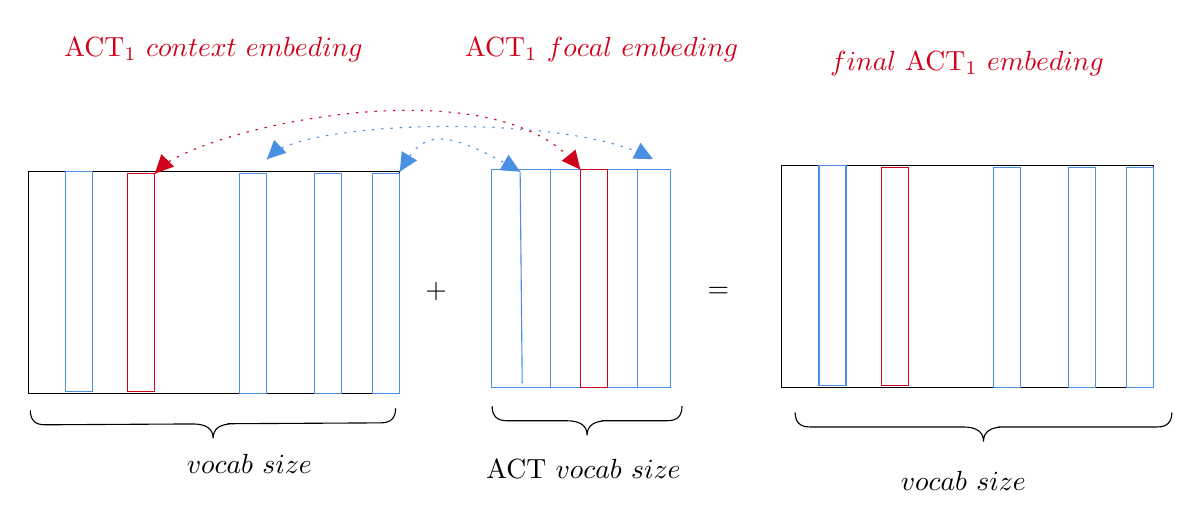
\begin{tikzpicture}[x=0.75pt,y=0.75pt,yscale=-1,xscale=1]
%uncomment if require: \path (0,370); %set diagram left start at 0, and has height of 370

\draw    (16.5, 126) rectangle (195.5, 233)   ;
\draw  [color={rgb, 255:red, 74; green, 144; blue, 226 }  ,draw opacity=1 ]  (239.75, 125) rectangle (326, 230)   ;
\draw   (17.5,241) .. controls (17.53,245.67) and (19.87,247.99) .. (24.54,247.96) -- (95.54,247.55) .. controls (102.21,247.51) and (105.55,249.82) .. (105.58,254.49) .. controls (105.55,249.82) and (108.87,247.47) .. (115.54,247.44)(112.54,247.45) -- (186.54,247.03) .. controls (191.21,247) and (193.53,244.66) .. (193.5,239.99) ;
\draw   (240,239) .. controls (240,243.67) and (242.33,246) .. (247,246) -- (275.75,246) .. controls (282.42,246) and (285.75,248.33) .. (285.75,253) .. controls (285.75,248.33) and (289.08,246) .. (295.75,246)(292.75,246) -- (324.5,246) .. controls (329.17,246) and (331.5,243.67) .. (331.5,239) ;
\draw  [color={rgb, 255:red, 208; green, 2; blue, 27 }  ,draw opacity=1 ]  (64.5, 127) rectangle (77.5, 232)   ;
\draw  [color={rgb, 255:red, 208; green, 2; blue, 27 }  ,draw opacity=1 ]  (282.5, 125) rectangle (295.5, 230)   ;
\draw   (386,242) .. controls (386,246.67) and (388.33,249) .. (393,249) -- (466.75,249) .. controls (473.42,249) and (476.75,251.33) .. (476.75,256) .. controls (476.75,251.33) and (480.08,249) .. (486.75,249)(483.75,249) -- (560.5,249) .. controls (565.17,249) and (567.5,246.67) .. (567.5,242) ;
\draw    (268, 125) rectangle (268, 230)   ;
\draw    (310.25, 125) rectangle (310.25, 229)   ;
\draw [color={rgb, 255:red, 74; green, 144; blue, 226 }  ,draw opacity=1 ]   (253.5,126) -- (254.5,228) ;


\draw [color={rgb, 255:red, 74; green, 144; blue, 226 }  ,draw opacity=1 ]   (268,125) -- (268,230) ;


\draw [color={rgb, 255:red, 74; green, 144; blue, 226 }  ,draw opacity=1 ]   (310.25,125) -- (310.25,230) ;


\draw [color={rgb, 255:red, 74; green, 144; blue, 226 }  ,draw opacity=1 ]   (326,125) -- (326,230) ;


\draw  [color={rgb, 255:red, 74; green, 144; blue, 226 }  ,draw opacity=1 ]  (118.5, 127) rectangle (131.5, 233)   ;
\draw  [color={rgb, 255:red, 74; green, 144; blue, 226 }  ,draw opacity=1 ]  (182.5, 127) rectangle (195.5, 233)   ;
\draw [color={rgb, 255:red, 74; green, 144; blue, 226 }  ,draw opacity=1 ] [dash pattern={on 0.84pt off 2.51pt}]  (195.5,126) .. controls (206.5,107) and (213.5,103) .. (253.5,126) ;
\draw [shift={(253.5,126)}, rotate = 209.57999999999998] [fill={rgb, 255:red, 74; green, 144; blue, 226 }  ,fill opacity=1 ] [draw opacity=0] (8.93,-4.29) -- (0,0) -- (8.93,4.29) -- (8.93,-4.29)    ;
\draw [shift={(195.5,126)}, rotate = 301.28] [fill={rgb, 255:red, 74; green, 144; blue, 226 }  ,fill opacity=1 ] [draw opacity=0] (8.93,-4.29) -- (0,0) -- (8.93,4.29) -- (8.93,-4.29)    ;
\draw [color={rgb, 255:red, 74; green, 144; blue, 226 }  ,draw opacity=1 ] [dash pattern={on 0.84pt off 2.51pt}]  (131.5,120) .. controls (142.5,101) and (277.5,97) .. (317.5,120) ;
\draw [shift={(317.5,120)}, rotate = 207.42000000000002] [fill={rgb, 255:red, 74; green, 144; blue, 226 }  ,fill opacity=1 ] [draw opacity=0] (8.93,-4.29) -- (0,0) -- (8.93,4.29) -- (8.93,-4.29)    ;
\draw [shift={(131.5,120)}, rotate = 316.16] [fill={rgb, 255:red, 74; green, 144; blue, 226 }  ,fill opacity=1 ] [draw opacity=0] (8.93,-4.29) -- (0,0) -- (8.93,4.29) -- (8.93,-4.29)    ;
\draw [color={rgb, 255:red, 208; green, 2; blue, 27 }  ,draw opacity=1 ] [dash pattern={on 0.84pt off 2.51pt}]  (77.5,127) .. controls (88.5,108) and (241.5,70) .. (282.5,125) ;
\draw [shift={(282.5,125)}, rotate = 230.89] [fill={rgb, 255:red, 208; green, 2; blue, 27 }  ,fill opacity=1 ] [draw opacity=0] (8.93,-4.29) -- (0,0) -- (8.93,4.29) -- (8.93,-4.29)    ;
\draw [shift={(77.5,127)}, rotate = 313.85] [fill={rgb, 255:red, 208; green, 2; blue, 27 }  ,fill opacity=1 ] [draw opacity=0] (8.93,-4.29) -- (0,0) -- (8.93,4.29) -- (8.93,-4.29)    ;
\draw  [color={rgb, 255:red, 74; green, 144; blue, 226 }  ,draw opacity=1 ]  (154.5, 127) rectangle (167.5, 233)   ;
\draw  [color={rgb, 255:red, 74; green, 144; blue, 226 }  ,draw opacity=1 ]  (34.5, 126) rectangle (47.5, 232)   ;
\draw    (379.5, 123) rectangle (558.5, 230)   ;
\draw  [color={rgb, 255:red, 208; green, 2; blue, 27 }  ,draw opacity=1 ]  (427.5, 124) rectangle (440.5, 229)   ;
\draw  [color={rgb, 255:red, 74; green, 144; blue, 226 }  ,draw opacity=1 ]  (481.5, 124) rectangle (494.5, 230)   ;
\draw  [color={rgb, 255:red, 74; green, 144; blue, 226 }  ,draw opacity=1 ]  (545.5, 124) rectangle (558.5, 230)   ;
\draw  [color={rgb, 255:red, 74; green, 144; blue, 226 }  ,draw opacity=1 ]  (517.5, 124) rectangle (530.5, 230)   ;
\draw  [color={rgb, 255:red, 74; green, 144; blue, 226 }  ,draw opacity=1 ]  (397.5, 123) rectangle (410.5, 229)   ;

\draw (124,186) node   {$\stackrel{}{}$};
\draw (213,184) node   {$+$};
\draw (349,184) node   {$=$};
\draw (123,267) node   {$vocab\ size$};
\draw (284,269) node   {$\mathrm{ACT}\ vocab\ size$};
\draw (108,67) node [color={rgb, 255:red, 208; green, 2; blue, 27 }  ,opacity=1 ]  {$\mathrm{ACT}_1\ context\ embeding\ $};
\draw (295,67) node [color={rgb, 255:red, 208; green, 2; blue, 27 }  ,opacity=1 ]  {$\mathrm{ACT}_1\ focal\ embeding\ $};
\draw (471,74) node [color={rgb, 255:red, 208; green, 2; blue, 27 }  ,opacity=1 ]  {$final\ \mathrm{ACT}_1\ embeding\ $};
\draw (467,275) node [color={rgb, 255:red, 0; green, 0; blue, 0 }  ,opacity=1 ]  {$vocab\ size$};
\draw (487,183) node   {$\stackrel{}{}$};


\end{tikzpicture}



}
\caption{Selectional addition of focal and context embedding in case of the actor embeddings. ACT$_1$ is shown as an example, where embeddings in focal and context matrices are combined to make the final embedding.} \label{fig:focal_addition}
\end{figure}

\begin{figure}
{\small 
\tikzset{every picture/.style={line width=0.75pt}} %set default line width to 0.75pt        

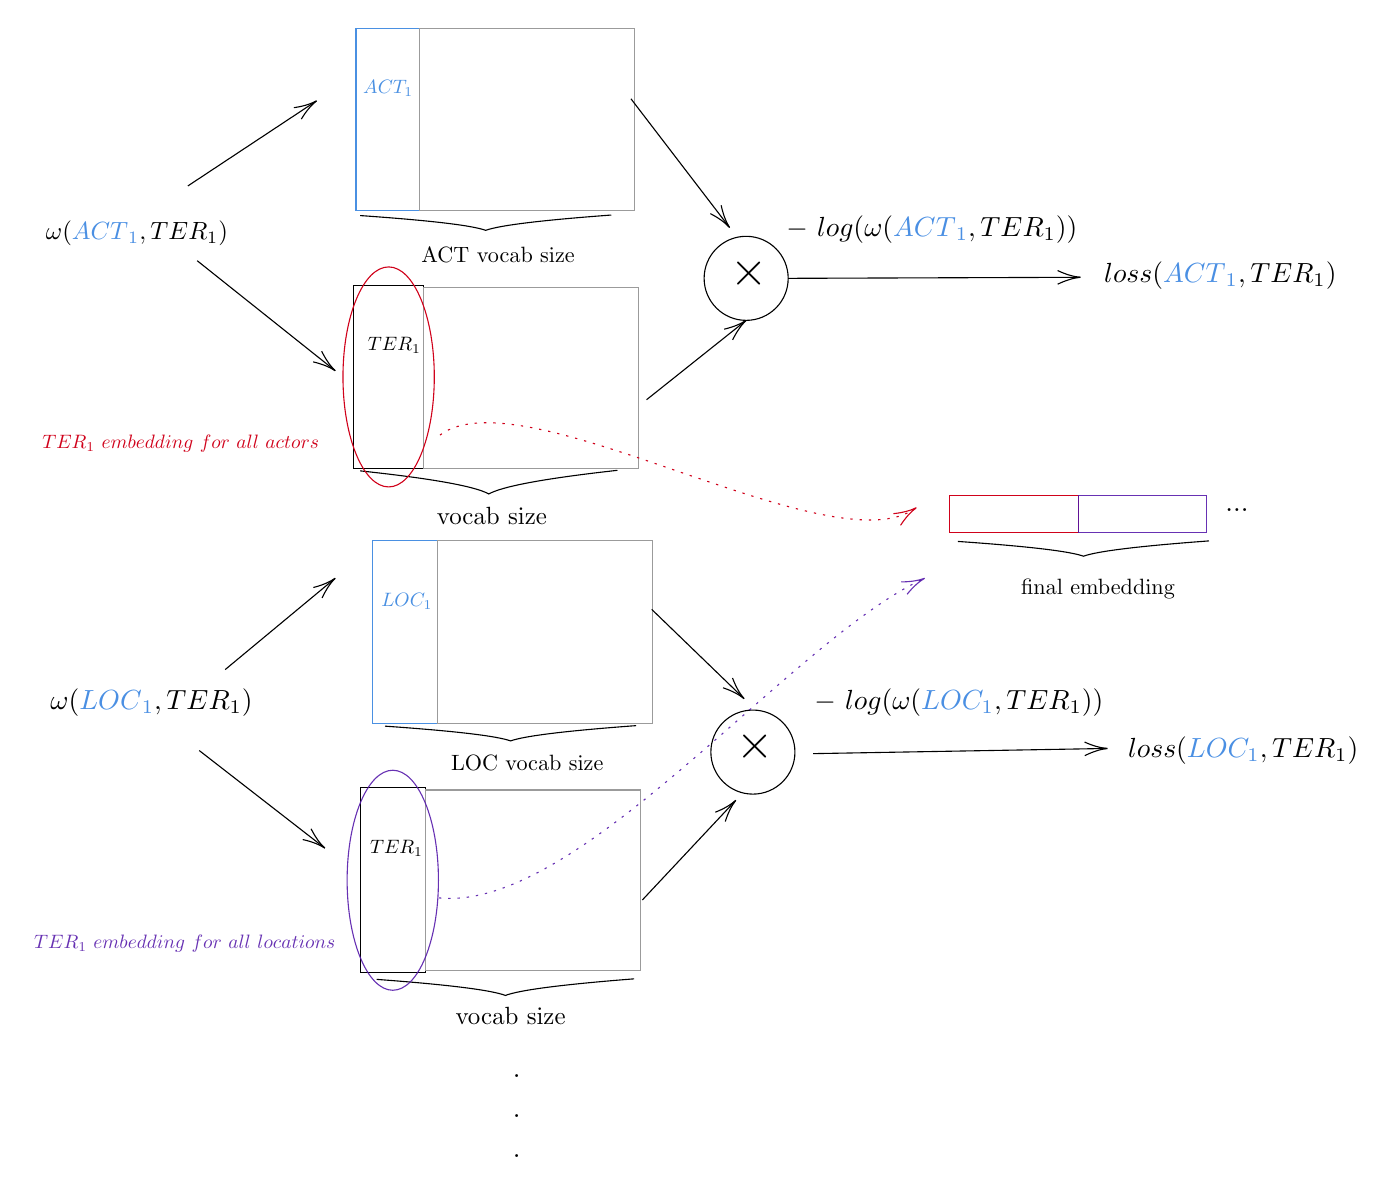
\begin{tikzpicture}[x=0.75pt,y=0.75pt,yscale=-1,xscale=1]
%uncomment if require: \path (0,573); %set diagram left start at 0, and has height of 573

\draw    (373.75,127.5) -- (514.5,127) ;
\draw [shift={(514.5,127)}, rotate = 539.8] [color={rgb, 255:red, 0; green, 0; blue, 0 }  ]   (0,0) .. controls (3.31,-0.3) and (6.95,-1.4) .. (10.93,-3.29)(0,0) .. controls (3.31,0.3) and (6.95,1.4) .. (10.93,3.29)   ;

\draw    (84.5,83) -- (146.5,42) ;
\draw [shift={(146.5,42)}, rotate = 506.52] [color={rgb, 255:red, 0; green, 0; blue, 0 }  ]   (0,0) .. controls (3.31,-0.3) and (6.95,-1.4) .. (10.93,-3.29)(0,0) .. controls (3.31,0.3) and (6.95,1.4) .. (10.93,3.29)   ;

\draw  [color={rgb, 255:red, 74; green, 144; blue, 226 }  ,draw opacity=1 ]  (165.5, 7) rectangle (196, 95)   ;
\draw    (164.5, 131) rectangle (198, 219)   ;
\draw  [color={rgb, 255:red, 155; green, 155; blue, 155 }  ,draw opacity=1 ]  (196, 7) rectangle (299.5, 95)   ;
\draw  [color={rgb, 255:red, 155; green, 155; blue, 155 }  ,draw opacity=1 ]  (198, 132) rectangle (301.5, 219)   ;
\draw [rotate around= { 89.88: (229.51, 225.75)
    }]  (223.89,163.75) .. controls (227.64,198.19) and (231.38,218.86) .. (235.13,225.75) .. controls (231.38,232.64) and (227.64,253.31) .. (223.89,287.75) ;
\draw [rotate around= { 89.88: (228.01, 100.75)
    }]  (224.39,40.25) .. controls (226.8,73.86) and (229.22,94.03) .. (231.63,100.75) .. controls (229.22,107.47) and (226.8,127.64) .. (224.39,161.25) ;
\draw    (353.5, 127.5) circle [x radius= 20.25, y radius= 20.25]  ;
\draw    (305.5,186) -- (353.5,147.75) ;
\draw [shift={(353.5,147.75)}, rotate = 501.45] [color={rgb, 255:red, 0; green, 0; blue, 0 }  ]   (0,0) .. controls (3.31,-0.3) and (6.95,-1.4) .. (10.93,-3.29)(0,0) .. controls (3.31,0.3) and (6.95,1.4) .. (10.93,3.29)   ;

\draw    (298,41) -- (345.5,103) ;
\draw [shift={(345.5,103)}, rotate = 232.54] [color={rgb, 255:red, 0; green, 0; blue, 0 }  ]   (0,0) .. controls (3.31,-0.3) and (6.95,-1.4) .. (10.93,-3.29)(0,0) .. controls (3.31,0.3) and (6.95,1.4) .. (10.93,3.29)   ;

\draw    (90,355) -- (150.5,402) ;
\draw [shift={(150.5,402)}, rotate = 217.84] [color={rgb, 255:red, 0; green, 0; blue, 0 }  ]   (0,0) .. controls (3.31,-0.3) and (6.95,-1.4) .. (10.93,-3.29)(0,0) .. controls (3.31,0.3) and (6.95,1.4) .. (10.93,3.29)   ;

\draw    (102.5,316) -- (155.5,272) ;
\draw [shift={(155.5,272)}, rotate = 500.3] [color={rgb, 255:red, 0; green, 0; blue, 0 }  ]   (0,0) .. controls (3.31,-0.3) and (6.95,-1.4) .. (10.93,-3.29)(0,0) .. controls (3.31,0.3) and (6.95,1.4) .. (10.93,3.29)   ;

\draw  [color={rgb, 255:red, 74; green, 144; blue, 226 }  ,draw opacity=1 ]  (173.5, 254) rectangle (205, 342)   ;
\draw    (167.5, 373) rectangle (199, 462)   ;
\draw  [color={rgb, 255:red, 155; green, 155; blue, 155 }  ,draw opacity=1 ]  (205, 254) rectangle (308.5, 342)   ;
\draw  [color={rgb, 255:red, 155; green, 155; blue, 155 }  ,draw opacity=1 ]  (199, 374) rectangle (302.5, 461)   ;
\draw [rotate around= { 89.88: (237.51, 469.07)
    }]  (233.57,407.07) .. controls (236.2,441.51) and (238.82,462.18) .. (241.44,469.07) .. controls (238.82,475.95) and (236.2,496.62) .. (233.57,531.07) ;
\draw    (356.75, 355.75) circle [x radius= 20.25, y radius= 20.25]  ;
\draw    (303.5,427) -- (348.5,379) ;
\draw [shift={(348.5,379)}, rotate = 493.15] [color={rgb, 255:red, 0; green, 0; blue, 0 }  ]   (0,0) .. controls (3.31,-0.3) and (6.95,-1.4) .. (10.93,-3.29)(0,0) .. controls (3.31,0.3) and (6.95,1.4) .. (10.93,3.29)   ;

\draw    (308,287) -- (352.5,330) ;
\draw [shift={(352.5,330)}, rotate = 224.02] [color={rgb, 255:red, 0; green, 0; blue, 0 }  ]   (0,0) .. controls (3.31,-0.3) and (6.95,-1.4) .. (10.93,-3.29)(0,0) .. controls (3.31,0.3) and (6.95,1.4) .. (10.93,3.29)   ;

\draw [rotate around= { 89.88: (240.01, 346.75)
    }]  (236.39,286.25) .. controls (238.8,319.86) and (241.22,340.03) .. (243.63,346.75) .. controls (241.22,353.47) and (238.8,373.64) .. (236.39,407.25) ;
\draw  [color={rgb, 255:red, 208; green, 2; blue, 27 }  ,draw opacity=1 ]  (181.25, 175) circle [x radius= 22, y radius= 53]  ;
\draw  [color={rgb, 255:red, 82; green, 21; blue, 168 }  ,draw opacity=0.88 ]  (183.25, 417.5) circle [x radius= 22, y radius= 53]  ;
\draw [color={rgb, 255:red, 208; green, 2; blue, 27 }  ,draw opacity=1 ] [dash pattern={on 0.84pt off 2.51pt}]  (206,203) .. controls (246,173) and (395.5,268) .. (435.5,238) ;
\draw [shift={(435.5,238)}, rotate = 508.65] [color={rgb, 255:red, 208; green, 2; blue, 27 }  ,draw opacity=1 ]   (0,0) .. controls (3.31,-0.3) and (6.95,-1.4) .. (10.93,-3.29)(0,0) .. controls (3.31,0.3) and (6.95,1.4) .. (10.93,3.29)   ;

\draw [color={rgb, 255:red, 82; green, 21; blue, 168 }  ,draw opacity=0.88 ] [dash pattern={on 0.84pt off 2.51pt}]  (205.5,426) .. controls (273.5,433) and (375.5,301) .. (439.5,272) ;
\draw [shift={(439.5,272)}, rotate = 514.4] [color={rgb, 255:red, 82; green, 21; blue, 168 }  ,draw opacity=0.88 ]   (0,0) .. controls (3.31,-0.3) and (6.95,-1.4) .. (10.93,-3.29)(0,0) .. controls (3.31,0.3) and (6.95,1.4) .. (10.93,3.29)   ;

\draw  [color={rgb, 255:red, 208; green, 2; blue, 27 }  ,draw opacity=1 ]  (451.5, 232) rectangle (513.5, 250)   ;
\draw  [color={rgb, 255:red, 82; green, 21; blue, 168 }  ,draw opacity=0.88 ]  (513.5, 232) rectangle (575.5, 250)   ;
\draw    (89,119) -- (155.5,172) ;
\draw [shift={(155.5,172)}, rotate = 218.55] [color={rgb, 255:red, 0; green, 0; blue, 0 }  ]   (0,0) .. controls (3.31,-0.3) and (6.95,-1.4) .. (10.93,-3.29)(0,0) .. controls (3.31,0.3) and (6.95,1.4) .. (10.93,3.29)   ;

\draw    (385.75,356.5) -- (527.5,354) ;
\draw [shift={(527.5,354)}, rotate = 538.99] [color={rgb, 255:red, 0; green, 0; blue, 0 }  ]   (0,0) .. controls (3.31,-0.3) and (6.95,-1.4) .. (10.93,-3.29)(0,0) .. controls (3.31,0.3) and (6.95,1.4) .. (10.93,3.29)   ;

\draw [rotate around= { 89.88: (516.01, 257.75)
    }]  (512.39,197.25) .. controls (514.8,230.86) and (517.22,251.03) .. (519.63,257.75) .. controls (517.22,264.47) and (514.8,284.64) .. (512.39,318.25) ;

\draw (60,106) node [scale=0.9] [align=left] {$\omega (\textcolor[rgb]{0.29,0.56,0.89}{ACT}\textcolor[rgb]{0.29,0.56,0.89}{_{1}} ,TER_{1})$};
\draw (181,36) node [scale=0.7,color={rgb, 255:red, 74; green, 144; blue, 226 }  ,opacity=1 ]  {$ACT_{1}$};
\draw (582,126) node  [align=left] {$loss(\textcolor[rgb]{0.29,0.56,0.89}{ACT}\textcolor[rgb]{0.29,0.56,0.89}{_{1}} ,TER_{1})$};
\draw (184,160) node [scale=0.7]  {$TER_{1}$};
\draw (234,116) node [scale=0.8] [align=left] {ACT vocab size};
\draw (231,242) node [scale=0.9] [align=left] {vocab size};
\draw (67,332) node  [align=left] {$\omega (\textcolor[rgb]{0.29,0.56,0.89}{LOC}\textcolor[rgb]{0.29,0.56,0.89}{_{1}} ,TER_{1})$};
\draw (190,283) node [scale=0.7,color={rgb, 255:red, 74; green, 144; blue, 226 }  ,opacity=1 ]  {$LOC_{1}$};
\draw (185,402) node [scale=0.7]  {$TER_{1}$};
\draw (248,361) node [scale=0.8] [align=left] {LOC vocab size};
\draw (240,483) node [scale=0.9] [align=left] {vocab size};
\draw (243,531) node  [align=left] {.\\.\\.};
\draw (81,207) node [scale=0.7,color={rgb, 255:red, 208; green, 2; blue, 27 }  ,opacity=1 ]  {$TER_{1} \ embedding\ for\ all\ actors$};
\draw (83,448) node [scale=0.7,color={rgb, 255:red, 82; green, 21; blue, 168 }  ,opacity=0.88 ]  {$TER_{1} \ embedding\ for\ all\ locations$};
\draw (590,239) node  [align=left] {...};
\draw (443,104) node  [align=left] {$-\ log( \omega (\textcolor[rgb]{0.29,0.56,0.89}{ACT}\textcolor[rgb]{0.29,0.56,0.89}{_{1}} ,TER_{1}))$};
\draw (593,355) node  [align=left] {$loss(\textcolor[rgb]{0.29,0.56,0.89}{LOC_{1}} ,TER_{1})$};
\draw (456,332) node  [align=left] {$-\ log( \omega (\textcolor[rgb]{0.29,0.56,0.89}{LOC_{1}} ,TER_{1}))$};
\draw (523,277) node [scale=0.8] [align=left] {final embedding};
\draw (355,125) node [scale=1.7280000000000002]  {$\times $};
\draw (358,353) node [scale=1.7280000000000002]  {$\times $};

\end{tikzpicture}



}
\caption{Faceted embedding with separate cost functions. Contains training of five different networks (two are shown in the figure) for a single input. The target word is TER$_1$, which is being trained against all actors, organisations, locations, dates and terms. The final embedding is created by concatenating the columns in the context embedding matrices that are associated with TER$_1$.} \label{fig:separate_cost}
\end{figure}
\begin{figure}
{\small 
\tikzset{every picture/.style={line width=0.75pt}} %set default line width to 0.75pt   

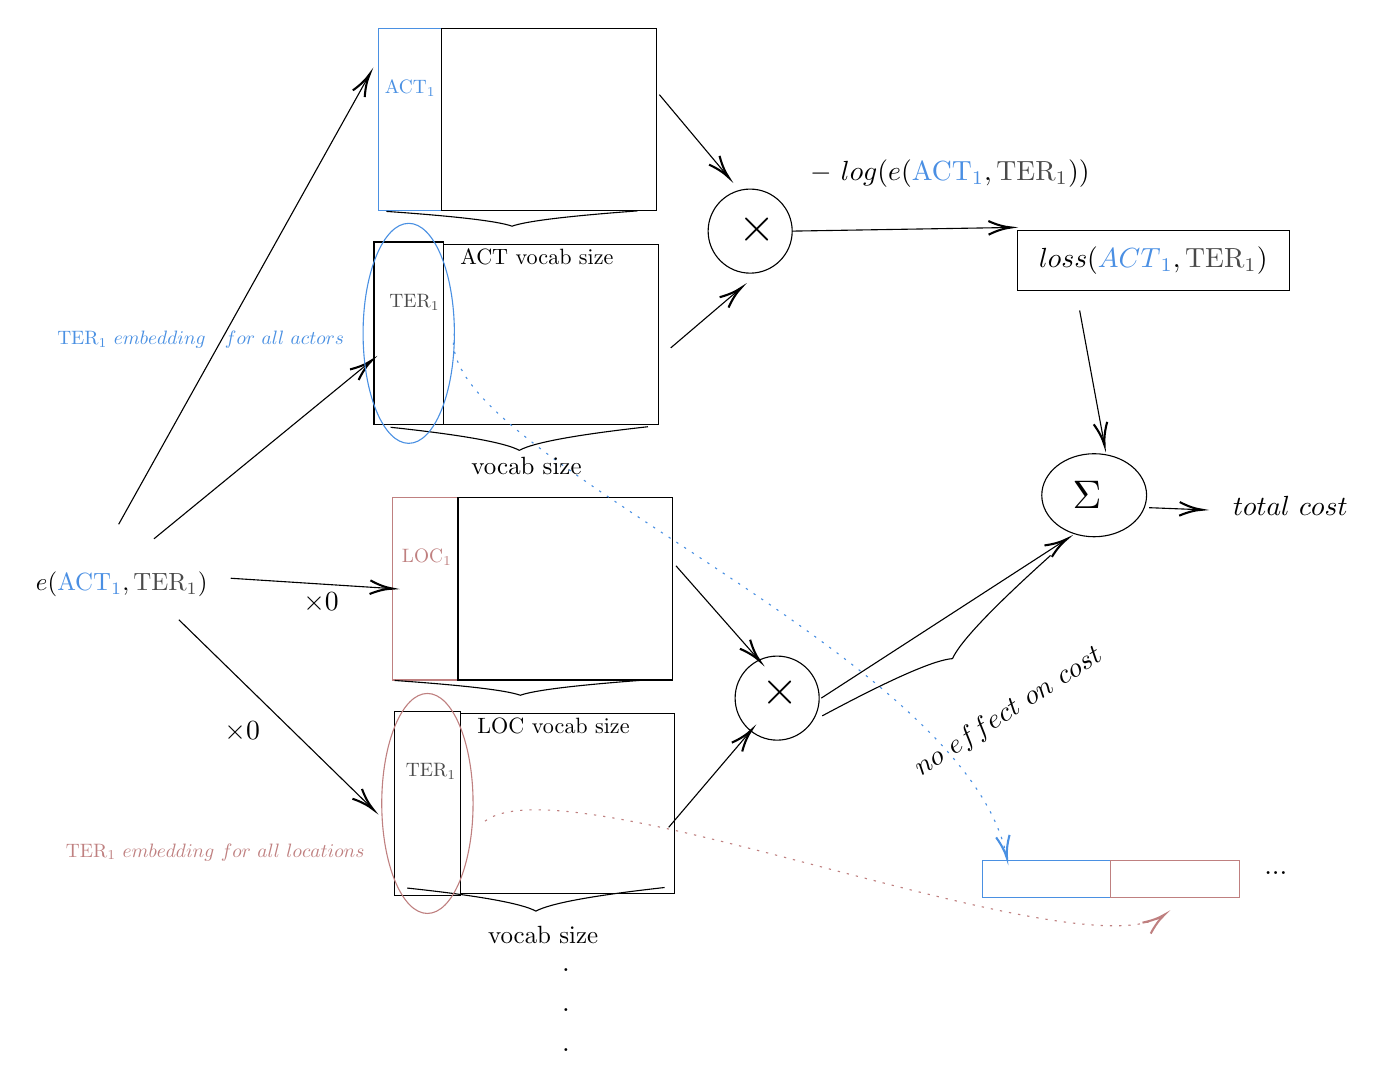
\begin{tikzpicture}[x=0.75pt,y=0.75pt,yscale=-1,xscale=1]
%uncomment if require: \path (0,547); %set diagram left start at 0, and has height of 547

%Straight Lines [id:da13430096728319052] 
\draw    (71.5,277) -- (174.95,192.27) ;
\draw [shift={(176.5,191)}, rotate = 500.68] [color={rgb, 255:red, 0; green, 0; blue, 0 }  ][line width=0.75]    (10.93,-3.29) .. controls (6.95,-1.4) and (3.31,-0.3) .. (0,0) .. controls (3.31,0.3) and (6.95,1.4) .. (10.93,3.29)   ;

%Straight Lines [id:da3395203365138022] 
\draw    (54.5,270) -- (174.53,54.75) ;
\draw [shift={(175.5,53)}, rotate = 479.14] [color={rgb, 255:red, 0; green, 0; blue, 0 }  ][line width=0.75]    (10.93,-3.29) .. controls (6.95,-1.4) and (3.31,-0.3) .. (0,0) .. controls (3.31,0.3) and (6.95,1.4) .. (10.93,3.29)   ;

%Shape: Rectangle [id:dp40988752111198234] 
\draw  [color={rgb, 255:red, 74; green, 144; blue, 226 }  ,draw opacity=1 ] (179.5,31) -- (210,31) -- (210,119) -- (179.5,119) -- cycle ;
%Shape: Rectangle [id:dp8120457242640955] 
\draw   (177.5,134) -- (211,134) -- (211,222) -- (177.5,222) -- cycle ;
%Shape: Rectangle [id:dp5994549314957651] 
\draw  [color={rgb, 255:red, 0; green, 0; blue, 0 }  ,draw opacity=1 ] (210,31) -- (313.5,31) -- (313.5,119) -- (210,119) -- cycle ;
%Shape: Rectangle [id:dp8953379233256253] 
\draw  [color={rgb, 255:red, 0; green, 0; blue, 0 }  ,draw opacity=1 ] (211,135) -- (314.5,135) -- (314.5,222) -- (211,222) -- cycle ;
\draw   (309.5,223) .. controls (275.06,226.82) and (254.4,230.61) .. (247.52,234.37) .. controls (240.63,230.64) and (219.95,226.93) .. (185.5,223.26) ;
\draw   (304.5,119) .. controls (270.9,121.49) and (250.73,123.94) .. (244.02,126.37) .. controls (237.29,123.97) and (217.12,121.6) .. (183.5,119.25) ;
%Shape: Ellipse [id:dp16021666171497673] 
\draw   (338.5,128.75) .. controls (338.5,117.57) and (347.57,108.5) .. (358.75,108.5) .. controls (369.93,108.5) and (379,117.57) .. (379,128.75) .. controls (379,139.93) and (369.93,149) .. (358.75,149) .. controls (347.57,149) and (338.5,139.93) .. (338.5,128.75) -- cycle ;
%Straight Lines [id:da010832594540308715] 
\draw    (320.5,185) -- (352.98,157.3) ;
\draw [shift={(354.5,156)}, rotate = 499.54] [color={rgb, 255:red, 0; green, 0; blue, 0 }  ][line width=0.75]    (10.93,-3.29) .. controls (6.95,-1.4) and (3.31,-0.3) .. (0,0) .. controls (3.31,0.3) and (6.95,1.4) .. (10.93,3.29)   ;

%Straight Lines [id:da7904695547993323] 
\draw    (315,63) -- (347.22,101.47) ;
\draw [shift={(348.5,103)}, rotate = 230.05] [color={rgb, 255:red, 0; green, 0; blue, 0 }  ][line width=0.75]    (10.93,-3.29) .. controls (6.95,-1.4) and (3.31,-0.3) .. (0,0) .. controls (3.31,0.3) and (6.95,1.4) .. (10.93,3.29)   ;

%Straight Lines [id:da40310566362864897] 
\draw    (517.5,167) -- (529.14,230.03) ;
\draw [shift={(529.5,232)}, rotate = 259.54] [color={rgb, 255:red, 0; green, 0; blue, 0 }  ][line width=0.75]    (10.93,-3.29) .. controls (6.95,-1.4) and (3.31,-0.3) .. (0,0) .. controls (3.31,0.3) and (6.95,1.4) .. (10.93,3.29)   ;

%Shape: Rectangle [id:dp7172146507008619] 
\draw  [color={rgb, 255:red, 191; green, 128; blue, 128 }  ,draw opacity=1 ] (186.5,257) -- (218,257) -- (218,345) -- (186.5,345) -- cycle ;
%Shape: Rectangle [id:dp060267406747659624] 
\draw   (187.5,360) -- (219,360) -- (219,449) -- (187.5,449) -- cycle ;
%Shape: Rectangle [id:dp6303673802072765] 
\draw  [color={rgb, 255:red, 0; green, 0; blue, 0 }  ,draw opacity=1 ] (218,257) -- (321.5,257) -- (321.5,345) -- (218,345) -- cycle ;
%Shape: Rectangle [id:dp304301296261714] 
\draw  [color={rgb, 255:red, 0; green, 0; blue, 0 }  ,draw opacity=1 ] (219,361) -- (322.5,361) -- (322.5,448) -- (219,448) -- cycle ;
\draw   (317.5,445) .. controls (283.06,448.82) and (262.4,452.61) .. (255.52,456.37) .. controls (248.63,452.64) and (227.95,448.93) .. (193.5,445.26) ;
%Shape: Ellipse [id:dp22428072345396544] 
\draw   (351.5,353.75) .. controls (351.5,342.57) and (360.57,333.5) .. (371.75,333.5) .. controls (382.93,333.5) and (392,342.57) .. (392,353.75) .. controls (392,364.93) and (382.93,374) .. (371.75,374) .. controls (360.57,374) and (351.5,364.93) .. (351.5,353.75) -- cycle ;
%Straight Lines [id:da29040700011246456] 
\draw    (319.5,416) -- (358.2,370.52) ;
\draw [shift={(359.5,369)}, rotate = 490.4] [color={rgb, 255:red, 0; green, 0; blue, 0 }  ][line width=0.75]    (10.93,-3.29) .. controls (6.95,-1.4) and (3.31,-0.3) .. (0,0) .. controls (3.31,0.3) and (6.95,1.4) .. (10.93,3.29)   ;

%Straight Lines [id:da7545042977801857] 
\draw    (323,290) -- (362.18,334.5) ;
\draw [shift={(363.5,336)}, rotate = 228.64] [color={rgb, 255:red, 0; green, 0; blue, 0 }  ][line width=0.75]    (10.93,-3.29) .. controls (6.95,-1.4) and (3.31,-0.3) .. (0,0) .. controls (3.31,0.3) and (6.95,1.4) .. (10.93,3.29)   ;

%Straight Lines [id:da13418076605656504] 
\draw    (393,353.75) -- (509.82,278.09) ;
\draw [shift={(511.5,277)}, rotate = 507.07] [color={rgb, 255:red, 0; green, 0; blue, 0 }  ][line width=0.75]    (10.93,-3.29) .. controls (6.95,-1.4) and (3.31,-0.3) .. (0,0) .. controls (3.31,0.3) and (6.95,1.4) .. (10.93,3.29)   ;

\draw   (308.5,345) .. controls (274.9,347.49) and (254.73,349.94) .. (248.02,352.37) .. controls (241.29,349.97) and (221.12,347.6) .. (187.5,345.25) ;
%Shape: Ellipse [id:dp1891084828946663] 
\draw  [color={rgb, 255:red, 74; green, 144; blue, 226 }  ,draw opacity=1 ] (172.25,178) .. controls (172.25,148.73) and (182.1,125) .. (194.25,125) .. controls (206.4,125) and (216.25,148.73) .. (216.25,178) .. controls (216.25,207.27) and (206.4,231) .. (194.25,231) .. controls (182.1,231) and (172.25,207.27) .. (172.25,178) -- cycle ;
%Shape: Ellipse [id:dp5133297466247488] 
\draw  [color={rgb, 255:red, 191; green, 128; blue, 128 }  ,draw opacity=1 ] (181.25,404.5) .. controls (181.25,375.23) and (191.1,351.5) .. (203.25,351.5) .. controls (215.4,351.5) and (225.25,375.23) .. (225.25,404.5) .. controls (225.25,433.77) and (215.4,457.5) .. (203.25,457.5) .. controls (191.1,457.5) and (181.25,433.77) .. (181.25,404.5) -- cycle ;
%Shape: Rectangle [id:dp8154703521346762] 
\draw  [color={rgb, 255:red, 74; green, 144; blue, 226 }  ,draw opacity=1 ] (470.5,432) -- (532.5,432) -- (532.5,450) -- (470.5,450) -- cycle ;
%Shape: Rectangle [id:dp3576905019222951] 
\draw  [color={rgb, 255:red, 191; green, 128; blue, 128 }  ,draw opacity=1 ] (532.5,432) -- (594.5,432) -- (594.5,450) -- (532.5,450) -- cycle ;
%Straight Lines [id:da3207889104512305] 
\draw    (108.5,296) -- (184.5,300.87) ;
\draw [shift={(186.5,301)}, rotate = 183.67] [color={rgb, 255:red, 0; green, 0; blue, 0 }  ][line width=0.75]    (10.93,-3.29) .. controls (6.95,-1.4) and (3.31,-0.3) .. (0,0) .. controls (3.31,0.3) and (6.95,1.4) .. (10.93,3.29)   ;

%Straight Lines [id:da444746435738554] 
\draw    (83.5,316) -- (175.82,406.1) ;
\draw [shift={(177.25,407.5)}, rotate = 224.3] [color={rgb, 255:red, 0; green, 0; blue, 0 }  ][line width=0.75]    (10.93,-3.29) .. controls (6.95,-1.4) and (3.31,-0.3) .. (0,0) .. controls (3.31,0.3) and (6.95,1.4) .. (10.93,3.29)   ;

\draw   (503.5,285) .. controls (475.52,310.16) and (459.77,326.73) .. (456.25,334.71) .. controls (447.55,335.32) and (426.62,344.52) .. (393.47,362.3) ;
%Shape: Ellipse [id:dp6408782289262511] 
\draw   (499.25,256) .. controls (499.25,244.95) and (510.55,236) .. (524.5,236) .. controls (538.45,236) and (549.75,244.95) .. (549.75,256) .. controls (549.75,267.05) and (538.45,276) .. (524.5,276) .. controls (510.55,276) and (499.25,267.05) .. (499.25,256) -- cycle ;
%Straight Lines [id:da19133214528940812] 
\draw    (379,128.75) -- (482.5,127.03) ;
\draw [shift={(484.5,127)}, rotate = 539.05] [color={rgb, 255:red, 0; green, 0; blue, 0 }  ][line width=0.75]    (10.93,-3.29) .. controls (6.95,-1.4) and (3.31,-0.3) .. (0,0) .. controls (3.31,0.3) and (6.95,1.4) .. (10.93,3.29)   ;

%Straight Lines [id:da406862365844594] 
\draw    (551,262) -- (574.5,262.92) ;
\draw [shift={(576.5,263)}, rotate = 182.25] [color={rgb, 255:red, 0; green, 0; blue, 0 }  ][line width=0.75]    (10.93,-3.29) .. controls (6.95,-1.4) and (3.31,-0.3) .. (0,0) .. controls (3.31,0.3) and (6.95,1.4) .. (10.93,3.29)   ;

%Curve Lines [id:da14396608756415818] 
\draw [color={rgb, 255:red, 191; green, 128; blue, 128 }  ,draw opacity=1 ] [dash pattern={on 0.84pt off 2.51pt}]  (231,413) .. controls (270.6,383.3) and (513.57,485.91) .. (557.24,458.86) ;
\draw [shift={(558.5,458)}, rotate = 503.13] [color={rgb, 255:red, 191; green, 128; blue, 128 }  ,draw opacity=1 ][line width=0.75]    (10.93,-3.29) .. controls (6.95,-1.4) and (3.31,-0.3) .. (0,0) .. controls (3.31,0.3) and (6.95,1.4) .. (10.93,3.29)   ;

%Curve Lines [id:da8005082280810756] 
\draw [color={rgb, 255:red, 74; green, 144; blue, 226 }  ,draw opacity=1 ] [dash pattern={on 0.84pt off 2.51pt}]  (216.25,178) .. controls (203.56,234.72) and (460.91,329.05) .. (482.2,429.49) ;
\draw [shift={(482.5,431)}, rotate = 259.35] [color={rgb, 255:red, 74; green, 144; blue, 226 }  ,draw opacity=1 ][line width=0.75]    (10.93,-3.29) .. controls (6.95,-1.4) and (3.31,-0.3) .. (0,0) .. controls (3.31,0.3) and (6.95,1.4) .. (10.93,3.29)   ;


% Text Node
\draw (195,60) node [scale=0.7,color={rgb, 255:red, 74; green, 144; blue, 226 }  ,opacity=1 ]  {$\mathrm{ACT}_{1}$};
% Text Node
\draw (362,128) node [scale=1.7280000000000002]  {$\times $};
% Text Node
\draw (197,163) node [scale=0.7,color={rgb, 255:red, 74; green, 74; blue, 74 }  ,opacity=1 ]  {$\mathrm{TER}_{1}$};
% Text Node
\draw (256,141) node [scale=0.8] [align=left] {ACT vocab size};
% Text Node
\draw (251,242) node [scale=0.9] [align=left] {vocab size};
% Text Node
\draw (203,286) node [scale=0.7,color={rgb, 255:red, 191; green, 128; blue, 128 }  ,opacity=1 ]  {$\mathrm{LOC}_{1}$};
% Text Node
\draw (205,389) node [scale=0.7,color={rgb, 255:red, 74; green, 74; blue, 74 }  ,opacity=1 ]  {$\mathrm{TER}_{1}$};
% Text Node
\draw (264,367) node [scale=0.8] [align=left] {LOC vocab size};
% Text Node
\draw (259,468) node [scale=0.9] [align=left] {vocab size};
% Text Node
\draw (270,504) node  [align=left] {.\\.\\.};
% Text Node
\draw (94,181) node [scale=0.7,color={rgb, 255:red, 74; green, 144; blue, 226 }  ,opacity=1 ]  {$\mathrm{TER}_{1} \ embedding\ \ \ for\ all\ actors$};
% Text Node
\draw (101,428) node [scale=0.7,color={rgb, 255:red, 191; green, 128; blue, 128 }  ,opacity=1 ]  {$\mathrm{TER}_{1} \ embedding\ for\ all\ locations$};
% Text Node
\draw (612,438) node  [align=left] {...};
% Text Node
\draw (114,370) node   {$\times 0$};
% Text Node
\draw (152,308) node   {$\times 0$};
% Text Node
\draw (483,360) node [rotate=-327.48]  {$ \begin{array}{l}
no\ effect\ on\ cost\\
\end{array}$};
% Text Node
\draw (521,256) node [scale=1.44]  {$\Sigma $};
% Text Node
\draw (373,351) node [scale=1.7280000000000002]  {$\times $};
% Text Node
\draw (56,299) node [scale=0.9] [align=left] {$e (\textcolor[rgb]{0.29,0.56,0.89}{\mathrm{ACT}}\textcolor[rgb]{0.29,0.56,0.89}{_{1}} ,\textcolor[rgb]{0.29,0.29,0.29}{\mathrm{TER}_{1}})$};
% Text Node
\draw    (487.5,128.5) -- (618.5,128.5) -- (618.5,157.5) -- (487.5,157.5) -- cycle  ;
\draw (553,143) node  [align=left] {$loss(\textcolor[rgb]{0.29,0.56,0.89}{ACT}\textcolor[rgb]{0.29,0.56,0.89}{_{1}} ,\textcolor[rgb]{0.29,0.29,0.29}{\mathrm{TER}_{1}})$};
% Text Node
\draw (455,101) node  [align=left] {$-\ log( e (\textcolor[rgb]{0.29,0.56,0.89}{\mathrm{ACT}}\textcolor[rgb]{0.29,0.56,0.89}{_{1}} ,\textcolor[rgb]{0.29,0.29,0.29}{\mathrm{TER}_{1}}))$};
% Text Node
\draw (619,261) node  [align=left] {$total\ cost$};


\end{tikzpicture}
\caption{Faceted embedding with unified cost function. Training for a single input is shown using only one network. The target word is TER$_1$, which is being trained against all actors, organisations, locations, dates and terms. While training, the weights related to actors are only updated if the input edge weight has the start node type of an actor. Meanwhile, the rest of the weights related to other entity-types are freezed. The final embedding is created by concatenating the columns in the context embedding matrices that are associated with TER$_1$.} \label{fig:unified_cost}
}
\end{figure}
 %%%%%%%%%%%%%%%%%%%%%%%%%%%%%%%%%%%%%%%%%%%%%%%%%%%%%%%%%%%%
  %%%%%%%%%%%%%%%%%%%%%%%%%%%%%%%%%%%%%%%%%%%%%%%%%%%%%%%%%%%%
\subsection{Vectorized faceted embeddings}
In order to speed up the model and use batch gradient descent we need to vectorize the cost function. In the following we go through the vectorization process for the embeddings with separate costs. The same idea can also be applied during the training of the unified cost function.\\
If we consider $W$ as the matrix of all focal embeddings and $\tilde{ W }$ as the matrix of all context embeddings stacked row-wise, then we can vectorize the model according to Equation~\ref{eq:vectorized}. 
\begin{equation}
J=(W \hat{  W }^{ \top } +B+\tilde{ B } -log{ X })^{ 2 }
\label{eq:vectorized}
\end{equation}
%The original GloVe model contains:
%\begin{itemize}
%\item $W \in R^{V \times M} $ for focal embeddings.
% \item $\tilde{ W }  \in R^{V \times M} $ for context embeddings.
%\item $B,\tilde{B} \in R^{V \times 1}$ biases for focal and context embeddings. 
%\item $X \in R^{V\times V} $ co-occurrence matrix of the whole vocabulary. 
%\end{itemize}
Unlike the original GloVe model, the dimensions of  $W$ and $\tilde{ W } $ are no longer equal as our weighted adjacency matrix is no longer symmetric $X \in R^{|V_f|\times |V|} $.  $V_f$ is the set of all focal words, which is defined by the input. If actors are the focal words then $V_f$ is the  of all actors in the vocabulary. The parameters of the model are as follows: 
\begin{itemize}
\item $W \in R^{|V_f| \times M} $ for focal embeddings.
 \item $\tilde{ W }  \in R^{|V| \times M} $ for context embeddings.
\item $B,\tilde{B} \in R^{|V_f| \times 1}$ biases for focal and context embeddings.
\item $X \in R^{|V_f|\times |V|} $ co-occurrence matrix of the whole vocabulary. 
\end{itemize}
Biases have to be added row-wise to the matrices to preserve the original cost function~\ref{eq:glove_cost}. As a consequence, they are transformed to column vectors in the size of the focal vocabulary. A visual comparison between the original GloVe model ($J_g$) and our faceted cost function ($J_f$) can be seen below, where the size of the vocabulary is indicated by $|V|=v$ and size of the focal vocabulary by $|V_f|=v_f$\\
\[J_{f}=\stackrel{\mbox{$W(v\times M)$ }}{%
    \begin{bmatrix}
    a_{11} & a_{12}  \cdots  a_{1M} \\
    a_{21} & a_{22}  \cdots  a_{2M} \\
    \vdots & \vdots  \ddots  \vdots \\
    a_{v1} & a_{v2}  \cdots  a_{vM}
    \end{bmatrix}%
  } .
  \stackrel{\mbox{$\tilde{W}^T(M \times v)$ }}{%
    \begin{bmatrix}
    a_{11} & a_{12}  \cdots  a_{1v} \\
    a_{21} & a_{22}  \cdots  a_{2v} \\
    \vdots & \vdots  \ddots  \vdots \\
    a_{M1} & a_{M2}  \cdots  a_{Mv}
    \end{bmatrix}%
  } +
  \stackrel{B( v \times 1)}{%
    \begin{bmatrix}
    e_1 \\
    e_2 \\
    \vdots \\
    e_{v}
    \end{bmatrix}%
   }
   +
  \stackrel{\tilde{B |V|\times 1)}}{%
    \begin{bmatrix}
    e_1 \\
    e_2 \\
    \vdots \\
    e_{v}
    \end{bmatrix}%
   }-
   \stackrel{\mbox{$logX(v \times v)$ }}{%
    \begin{bmatrix}
    a_{11} & a_{12}  \cdots  a_{1v} \\
    a_{21} & a_{22}  \cdots  a_{2v} \\
    \vdots & \vdots  \ddots  \vdots \\
    a_{v1} & a_{v2}  \cdots  a_{vv}
    \end{bmatrix}%
  }
\]
\\
\[J_{f} =\stackrel{\mbox{$W( v_{f}\times M)$ }}{%
    \begin{bmatrix}
    a_{11} & a_{12}  \cdots  a_{1M} \\
    a_{21} & a_{22}  \cdots  a_{2M} \\
    \vdots & \vdots  \ddots  \vdots \\
    a_{v1} & a_{v2}  \cdots  a_{v
_{e}M}
    \end{bmatrix}%
  } .
  \stackrel{\mbox{$\tilde{W}^T(M \times |V|)$ }}{%
    \begin{bmatrix}
    a_{11} & a_{12}  \cdots  a_{1v} \\
    a_{21} & a_{22} \cdots  a_{2v} \\
    \vdots & \vdots \ddots \vdots \\
    a_{M1} & a_{M2}  \cdots  a_{Mv}
    \end{bmatrix}%
  } +
  \stackrel{B( v_{f}\times 1)}{%
    \begin{bmatrix}
    e_1 \\
    e_2 \\
    \vdots \\
    e_{v_{f}}
    \end{bmatrix}%
   }
   +
  \stackrel{\tilde{B}(v_{f}\times 1)}{%
    \begin{bmatrix}
    e_1 \\
    e_2 \\
    \vdots \\
    e_{v_{f}}
    \end{bmatrix}%
   }-
   \stackrel{\mbox{$logX( v_{f}\ \times v)$ }}{%
    \begin{bmatrix}
    a_{11} & a_{12}  \cdots  a_{1v} \\
    a_{21} & a_{22}  \cdots  a_{2v} \\
    \vdots & \vdots  \ddots  \vdots \\
    a_{v1} & a_{v2}  \cdots  a_{v_{f}v}
    \end{bmatrix}%
  }
\]

\section{Faceted Word2vec}\label{sec:faceted_word2vec}
Word embeddings are used as input features in many NLP tasks. Although methods like word2vec capture semantic features well, they often lack task-specific features. Thus, many studies focus on modifying and tweaking the existing methods for certain tasks, such as text classification~\brackettext{\cite{DBLP:conf/coling/LiuHGWTL18}}, semantic relation classification~\brackettext{\cite{DBLP:conf/conll/HashimotoSMT15}} and dependency parsing~\brackettext{\cite{DBLP:conf/acl/BansalGL14}}. Since with faceted embedding we also aim to modify existing methods to match our specific task, we looked a wide range of litreture on modifications of word embedding methods. In $2014$, Levy and Goldberg proposed a method to generalize the skip-gram achitecure of word2vec to include arbitrary contexts and used it to create dependency based embeddings~\brackettext{\cite{DBLP:conf/acl/LevyG14}}. We use the idea behind this model to define our own context for the skip-gram model, which allows us to learn the separate components of the faceted embedding. In this section, first, we give a brief description of embeddings with arbitrary contexts by Levy and Goldberg. Then, we look at our definition of context and modifications to the original model. Finally, we use this knowledge to generate the algorithm faceted word2vec. The model proposed by Levy and Goldberg uses the skip-gram architecture, thus, we also generate the faceted word2vec based on skip-gram and do not use the CBOW architecture.\\
For creating the faceted model using embeddings with arbitrary contexts, we follow these four steps: 
\begin{enumerate}        
 \item Extraction of type-specific edge lists from the co-occurrence graph, discussed in Section~\ref{sec:edges_as_pairs}.
 \item Training a low dimensional embedding for each edge list using the method proposed by  Levy and Goldberg, where the focal context pairs are edges of the graph~\brackettext{\cite{DBLP:conf/acl/LevyG14}}, discussed in Section~\ref{sec:arbitarty_context}.
 \item Disregarding the focal embeddings and keeping only the context embeddings, as it represents the relation of a word to entities of a specific type. 
 \item Concatenating the context embedding of all types to create the final embedding. 
 \end{enumerate}
 %%%%%%%%%%%%%%%%%%%%%%%%%%%%%%%%%%%%%%%%%%%%%%%%%%%%%%%%%%%%
\subsection{Embeddings with arbitrary contexts}\label{sec:arbitarty_context}
The general principle behind skip-gram is to bring words that appear in similar contexts in the text, closer in embedding space, where the contexts of a word are the words surrounding it. Therefore, the context vocabulary $C$ is identical to the complete word vocabulary $V$. In other words, the focal words and their context share the same vocabulary. Nonetheless, for embeddings with arbitrary contexts, this restriction is not required. The context does not need to correspond to words and can be defined based on the use-case, which is an important attribute for the faceted model. The negative sampling objective of word2vec, shown in Equation~\ref{eq:w2v_negative}, assumes a dataset $Q$ of focal and context pairs $(f,c)$ from a large body of text and samples negative examples form $\overline{Q}$. The model assigns a low score to the random negative samples and a high score to the real focal and context pairs. Since the input of the model is word pairs, it can be constructed in an arbitrary way. Levy and Goldberg specifically look at contexts, based on the syntactic relations, where the context is defined by the type of the dependency relation between the head and the modifier. They scan the text once and create focal and context pairs based on specific dependency relations and then use the generated pairs as positive inputs. For each $(f,c) \in Q$, $n$ samples $(f,c_1),\dots,(f,c_n)$ are constructed as negative examples, where $c_j$ is drawn according to its unigram distribution raised to the power of $\frac{3}{4}$~\brackettext{\cite{DBLP:conf/acl/LevyG14}}. Their framework is not only limited to dependency relations but also allows for various context definitions\cite{SCHOL:website/Levy2014}. Following their example, we can define a type-specific context to generate faceted embeddings. We denoted the faceted word2vec model by $f$W2V, where $f$ indicates the faceted model. In the following section, we show how the edges of co-occurrence graphs are used as focal and context pairs for our study.
 %%%%%%%%%%%%%%%%%%%%%%%%%%%%%%%%%%%%%%%%%%%%%%%%%%%%%%%%%%%%
\subsection{Edges of co-occurrence graphs as focal and context pairs}\label{sec:edges_as_pairs}
We take advantage of the definition of arbitrary context and define our context based on the types of entities surrounding a word. Our goal is to create embeddings, such that each part corresponds to the word related to the specific type of entities and a co-occurrence graph extracted from annotated text can help us achieve just that. To obtain each part of the embedding we define a type-specific edge list, in a similar fashion as type-specific adjacency matrices for faceted GloVe, where the start nodes are entities of a specific type and end nodes can be any term or entity from the vocabulary. More formally, in the heterogeneous graph $G=(V,E)$, where $V=A\bigcup  L\bigcup  \bigcup  O\bigcup  D\bigcup T $ is the set of all nodes with types actors, locations, organisations, dates, and any non-entity word (term) and $E$ is the set of all weighted edges, we extract the edge list where the start node is one of the types in set $V$. An example of the edge lists is shown in Figure~\ref{fig:facettedword2vec}. As demonstrated in Figure~\ref{fig:facettedword2vec}, we have a different edge list for each type. These edge lists can be treated as a focal and context pairs $(f,c)$ for the input of embeddings with arbitrary contexts, where $c \in V$ and $a$ is a specific type, e.g, $f \in A$ for generating actor part of the embedding. Thus, the focal and context vocabulary are not equal, as the focal vocabulary is always a subset of the context ($A \subset  V$). 
\begin{figure}
\centering 
\resizebox{0.80\textwidth}{0.28\textwidth}{      
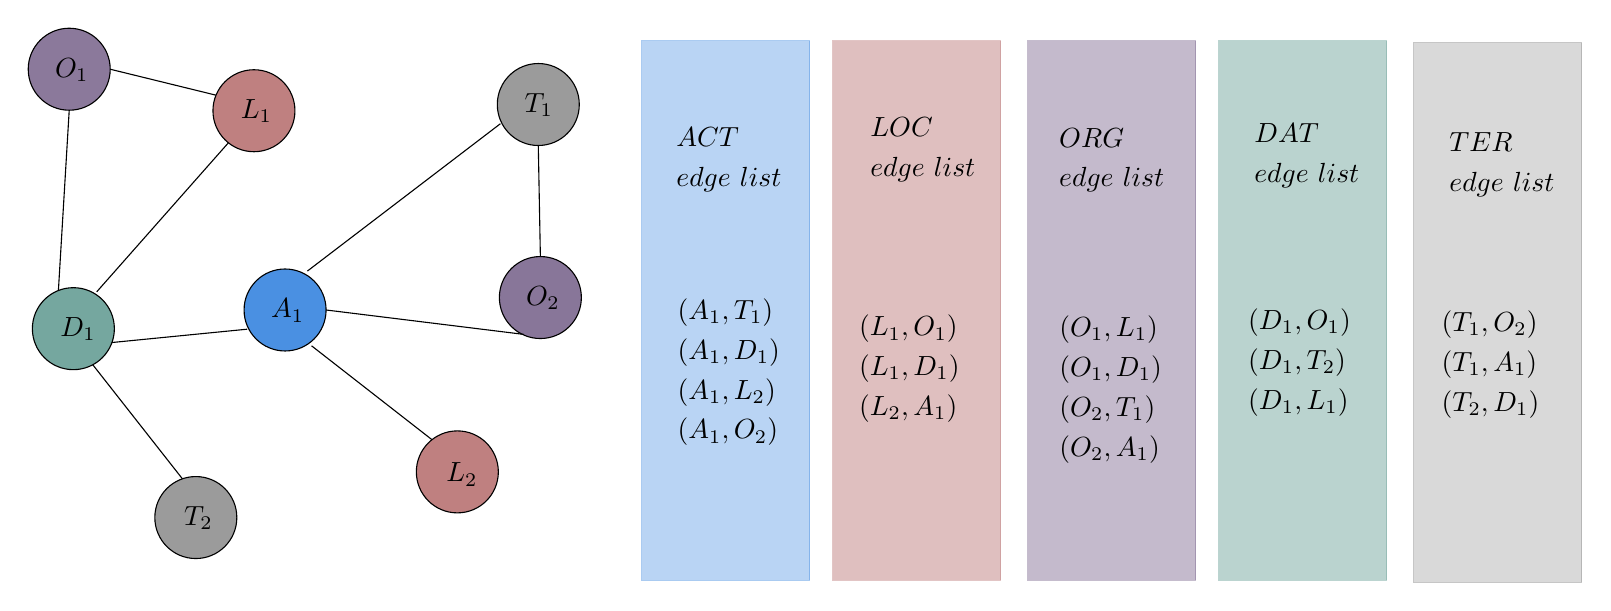
\begin{tikzpicture}[x=0.75pt,y=0.75pt,yscale=-1,xscale=1]
%uncomment if require: \path (0,324); %set diagram left start at 0, and has height of 324

%Shape: Circle [id:dp7723989663764896] 
\draw  [fill={rgb, 255:red, 120; green, 99; blue, 139 }  ,fill opacity=0.86 ] (24,56.75) .. controls (24,45.84) and (32.84,37) .. (43.75,37) .. controls (54.66,37) and (63.5,45.84) .. (63.5,56.75) .. controls (63.5,67.66) and (54.66,76.5) .. (43.75,76.5) .. controls (32.84,76.5) and (24,67.66) .. (24,56.75) -- cycle ;
%Straight Lines [id:da631891041159494] 
\draw    (269.75,93.5) -- (270.75,147) ;


%Straight Lines [id:da4375886533634059] 
\draw    (63.5,56.75) -- (117.5,70) ;


%Straight Lines [id:da6613925859828091] 
\draw    (121.5,91) -- (57,164) ;


%Straight Lines [id:da39535906402000176] 
\draw    (129.5,182) -- (58.5,189) ;


%Straight Lines [id:da6929421363539265] 
\draw    (55,199) -- (104.5,262) ;


%Straight Lines [id:da7460610286620943] 
\draw    (160.5,190) -- (219.5,236) ;


%Straight Lines [id:da9790672124174229] 
\draw    (251.5,83) -- (158.5,154) ;


%Straight Lines [id:da63778288309677] 
\draw    (38.5,164) -- (43.75,76.5) ;


%Shape: Circle [id:dp5787703304890821] 
\draw  [fill={rgb, 255:red, 117; green, 167; blue, 159 }  ,fill opacity=1 ] (26,181.75) .. controls (26,170.84) and (34.84,162) .. (45.75,162) .. controls (56.66,162) and (65.5,170.84) .. (65.5,181.75) .. controls (65.5,192.66) and (56.66,201.5) .. (45.75,201.5) .. controls (34.84,201.5) and (26,192.66) .. (26,181.75) -- cycle ;
%Shape: Circle [id:dp2977758613059365] 
\draw  [fill={rgb, 255:red, 191; green, 128; blue, 128 }  ,fill opacity=1 ] (113,76.75) .. controls (113,65.84) and (121.84,57) .. (132.75,57) .. controls (143.66,57) and (152.5,65.84) .. (152.5,76.75) .. controls (152.5,87.66) and (143.66,96.5) .. (132.75,96.5) .. controls (121.84,96.5) and (113,87.66) .. (113,76.75) -- cycle ;
%Shape: Circle [id:dp8211852276895382] 
\draw  [fill={rgb, 255:red, 74; green, 144; blue, 226 }  ,fill opacity=1 ] (128,172.75) .. controls (128,161.84) and (136.84,153) .. (147.75,153) .. controls (158.66,153) and (167.5,161.84) .. (167.5,172.75) .. controls (167.5,183.66) and (158.66,192.5) .. (147.75,192.5) .. controls (136.84,192.5) and (128,183.66) .. (128,172.75) -- cycle ;
%Shape: Circle [id:dp7755720350359876] 
\draw  [fill={rgb, 255:red, 155; green, 155; blue, 155 }  ,fill opacity=1 ] (85,272.75) .. controls (85,261.84) and (93.84,253) .. (104.75,253) .. controls (115.66,253) and (124.5,261.84) .. (124.5,272.75) .. controls (124.5,283.66) and (115.66,292.5) .. (104.75,292.5) .. controls (93.84,292.5) and (85,283.66) .. (85,272.75) -- cycle ;
%Shape: Circle [id:dp8914724887147505] 
\draw  [fill={rgb, 255:red, 155; green, 155; blue, 155 }  ,fill opacity=1 ] (250,73.75) .. controls (250,62.84) and (258.84,54) .. (269.75,54) .. controls (280.66,54) and (289.5,62.84) .. (289.5,73.75) .. controls (289.5,84.66) and (280.66,93.5) .. (269.75,93.5) .. controls (258.84,93.5) and (250,84.66) .. (250,73.75) -- cycle ;
%Shape: Circle [id:dp06424977358736528] 
\draw  [fill={rgb, 255:red, 191; green, 128; blue, 128 }  ,fill opacity=1 ] (211,250.75) .. controls (211,239.84) and (219.84,231) .. (230.75,231) .. controls (241.66,231) and (250.5,239.84) .. (250.5,250.75) .. controls (250.5,261.66) and (241.66,270.5) .. (230.75,270.5) .. controls (219.84,270.5) and (211,261.66) .. (211,250.75) -- cycle ;
%Shape: Circle [id:dp5224682342118112] 
\draw  [fill={rgb, 255:red, 120; green, 99; blue, 139 }  ,fill opacity=0.88 ] (251,166.75) .. controls (251,155.84) and (259.84,147) .. (270.75,147) .. controls (281.66,147) and (290.5,155.84) .. (290.5,166.75) .. controls (290.5,177.66) and (281.66,186.5) .. (270.75,186.5) .. controls (259.84,186.5) and (251,177.66) .. (251,166.75) -- cycle ;
%Straight Lines [id:da168907494889315] 
\draw    (262.75,184.5) -- (167.5,172.75) ;


%Shape: Rectangle [id:dp4597340173200979] 
\draw  [color={rgb, 255:red, 74; green, 144; blue, 226 }  ,draw opacity=0.47 ][fill={rgb, 255:red, 74; green, 144; blue, 226 }  ,fill opacity=0.39 ] (319.5,43) -- (400.5,43) -- (400.5,303) -- (319.5,303) -- cycle ;
%Shape: Rectangle [id:dp8236283831060471] 
\draw  [color={rgb, 255:red, 191; green, 128; blue, 128 }  ,draw opacity=0.46 ][fill={rgb, 255:red, 191; green, 128; blue, 128 }  ,fill opacity=0.5 ] (411.5,43) -- (492.5,43) -- (492.5,303) -- (411.5,303) -- cycle ;
%Shape: Rectangle [id:dp9350536299021817] 
\draw  [color={rgb, 255:red, 120; green, 99; blue, 139 }  ,draw opacity=0.43 ][fill={rgb, 255:red, 120; green, 99; blue, 139 }  ,fill opacity=0.44 ] (505.5,43) -- (586.5,43) -- (586.5,303) -- (505.5,303) -- cycle ;
%Shape: Rectangle [id:dp287143176572378] 
\draw  [color={rgb, 255:red, 117; green, 167; blue, 159 }  ,draw opacity=0.49 ][fill={rgb, 255:red, 117; green, 167; blue, 159 }  ,fill opacity=0.5 ] (597.5,43) -- (678.5,43) -- (678.5,303) -- (597.5,303) -- cycle ;
%Shape: Rectangle [id:dp42566484032417296] 
\draw  [color={rgb, 255:red, 155; green, 155; blue, 155 }  ,draw opacity=0.57 ][fill={rgb, 255:red, 155; green, 155; blue, 155 }  ,fill opacity=0.38 ] (691.5,44) -- (772.5,44) -- (772.5,304) -- (691.5,304) -- cycle ;

% Text Node
\draw (45,57) node   {$O_{1}$};
% Text Node
\draw (48,182) node   {$D_{1}$};
% Text Node
\draw (134,77) node   {$L_{1}$};
% Text Node
\draw (149,173) node   {$A_{1}$};
% Text Node
\draw (106,273) node   {$T_{2}$};
% Text Node
\draw (270,74) node   {$T_{1}$};
% Text Node
\draw (233,252) node   {$L_{2}$};
% Text Node
\draw (272,167) node   {$O_{2}$};
% Text Node
\draw (361.56,99.77) node   {$ \begin{array}{l}
ACT\ \\
edge\ list
\end{array}$};
% Text Node
\draw (455,95) node   {$ \begin{array}{l}
LOC\ \\
edge\ list
\end{array}$};
% Text Node
\draw (546,100) node   {$ \begin{array}{l}
ORG\ \\
edge\ list
\end{array}$};
% Text Node
\draw (640,98) node   {$ \begin{array}{l}
DAT\\
edge\ list
\end{array}$};
% Text Node
\draw (734,102) node   {$ \begin{array}{l}
TER\ \\
edge\ list
\end{array}$};
% Text Node
\draw (361.52,202.22) node   {$ \begin{array}{l}
( A_{1} ,T_{1})\\
( A_{1} ,D_{1})\\
( A_{1} ,L_{2})\\
( A_{1} ,O_{2})
\end{array}$};
% Text Node
\draw (448.52,210.22) node   {$ \begin{array}{l}
( L_{1} ,O_{1})\\
( L_{1} ,D_{1})\\
( L_{2} ,A_{1})\\
\\
\end{array}$};
% Text Node
\draw (545.52,220.22) node   {$ \begin{array}{l}
( O_{1} ,L_{1})\\
( O_{1} ,D_{1})\\
( O_{2} ,T_{1})\\
( O_{2} ,A_{1})\\
\\
\end{array}$};
% Text Node
\draw (636.52,207.22) node   {$ \begin{array}{l}
( D_{1} ,O_{1})\\
( D_{1} ,T_{2})\\
( D_{1} ,L_{1})\\
\\
\end{array}$};
% Text Node
\draw (728.52,208.22) node   {$ \begin{array}{l}
( T_{1} ,O_{2})\\
( T_{1} ,A_{1})\\
( T_{2} ,D_{1})\\
\\
\end{array}$};


\end{tikzpicture}
}
\caption{An example of creating type specific edge lists for a graph with node type: actor (A), location (L), organisation (L), date (D), and term (T).}
\label{fig:facettedword2vec}
\end{figure} 
Based on each edge list the model learns a separate embedding, with entities of a certain type as focal words and the rest of the vocabulary as context. As a result, each context embedding encodes the relation of the complete vocabulary with a certain type. For example, if we look at the context embedding for actors, it encodes the relation of the words in the vocabulary to all the actors. Naturally, if a word does not have an edge to any actor it will not be present in the context embeddings. For such cases, it makes sense to set the actor part of that word equal to a vector of zeros. For example, in Figure~\ref{fig:facettedword2vec}, $T_2$ will only have a non-zero date component and the rest are set to zero. This approach has some drawbacks, as the cosine similarity between a vector of zero and any other vector is undefined. Therefore, if a component of a vector is set to zero, that word becomes incomparable to all other words in that sub-space. It also causes  problems for clustering algorithms that require a distance measure between the points, if the cosine similarity is undefined, then we are unable to compare the words and form clusters. To solve this issue, we add a small number $0.0001$ to the vectors of all zero, mapping all the words to the same point, while keeping the component small. Moreover, clustering algorithms are able to compute the distance between the word vectors in the sub-spaces.This approach also has some unwanted implications,  if components of two word are identical, their cosine similarity is always one. Thus, any point that does not have relations to entities of a particular type are considered similar in that subspace, which is not always the case. For example, in Figure~\ref{fig:facettedword2vec}, $T_2$ and $L_2$ both have the same organisation component, as they are not connected to any organisation node. The absence of an edge to a organisation does not necessary mean that $T_2$ and $L_2$ should be similar in organisation space, which is what the model would imply. 
 %%%%%%%%%%%%%%%%%%%%%%%%%%%%%%%%%%%%%%%%%%%%%%%%%%%%%%%%%%%%

 %%%%%%%%%%%%%%%%%%%%%%%%%%%%%%%%%%%%%%%%%%%%%%%%%%%%%%%%%%%%
\section{Faceted DeepWalk}\label{sec:faceted_deepwalk}
Another way to achieve the faceted model is by taking advantage of the type-restricted random walks. For this purpose, we alter the DeepWalk model to meet our needs. In $2017$, \emph{metapath2vec} was proposed by Dong et al. to study representation learning in heterogeneous graphs with multiple edge and node types, such as coauthor relationships graphs~\brackettext{\cite{DBLP:conf/kdd/DongCS17}}. Metapath2vec learns a low dimensional representation of the graph using random walks that are restricted to the only transition between particular types of nodes and edges. They also introduce a heterogeneous skip-gram which maximizes the probability of having the heterogeneous context for a given node~\brackettext{\cite{DBLP:journals/tkde/CaiZC18}}. For learning the faceted embeddings, however, we take a more straightforward approach. We take advantage of the weighted random walks used in Chapter~\ref{chap:entity} to generate entity embeddings to introduce a new type-restricted random walk to restrict the context of a word to certain entity type. 
In general, faceted DeepWalk model consists of three steps: 
\begin{enumerate}
\item Generating type specific corpus based on type-restricted fixed length random walks starting from all the nodes in the graphs.
\item Applying the skip-gram model on the random walk corpora. 
\item Concatenating the resulting embedding for each type to achieve the final faceted model.  
\end{enumerate}
\emph{Type-restricted random walk:} Formally, a type-restricted random walk in graph $G=(V,E)$ is denoted in the form of $v_1 \rightarrow v_2 \rightarrow v_3\rightarrow \dots \rightarrow t_n$, where the nodes $t_i$ belong to a certain node type. In a graph, where $V=A\bigcup  L\bigcup  O\bigcup  D\bigcup  T$, to sample only locations related to a node, we perform a location-restricted random walk. Consequently, the transition probability for the restricted type $L$ between node $i$ and $j$ in a weighted graph is defined in Equation ~\ref{eq:transition_type_restricted}, where $e_{i,j}$ is the edge weight between the two nodes $i$ and $j$. Given that we are removing the possibility of transitioning to any type other than the pre-defined one, the probabilities are normalized by the summation of the edge weight of the pre-defined type.
\begin{equation}
P_{ i,j }=\left\{ 
\begin{matrix}
 \frac { f(e_{ i,j }) }{ \sum _{ k\in L,f(e_{ k })\in E_{ i } }^{  }{ f(e_{ k }) }  }  & \mathrm{if}\quad j\in L \\
0 & \mathrm{if}\quad j\notin L
\end{matrix} 
\right. 
\label{eq:transition_type_restricted}
\end{equation} 
\noindent
Function $f$ is the edge normalization function. Like entity embeddings, we use two normalization functions: \\
\begin{enumerate}
\item  $f=\mathrm{id}$, identity function. We denote these models by $f$DW$_{id}$, where $id$ shows the identity mapping. \\
\item  $f=\log$, logarithmic normalization. These models are denoted by  $f$DW$_{log}$.\\
\end{enumerate}
\noindent
An example of the type-restricted random walk for type location is illustrated in Figure~\ref{fig:facetteddeepwalk}. Any nodes in the random walk have to be a location to be visited, otherwise, it is disregard. Hence, by creating a type specific corpus with the type-restricted random walk, we can train a skip-gram model that learns the representation of all nodes with regards to a single entity type. By repeating this process for all node types and concatenating the results we achieve the faceted model.
\begin{figure}
\centering 
\resizebox{0.60\textwidth}{0.27\textwidth}{      
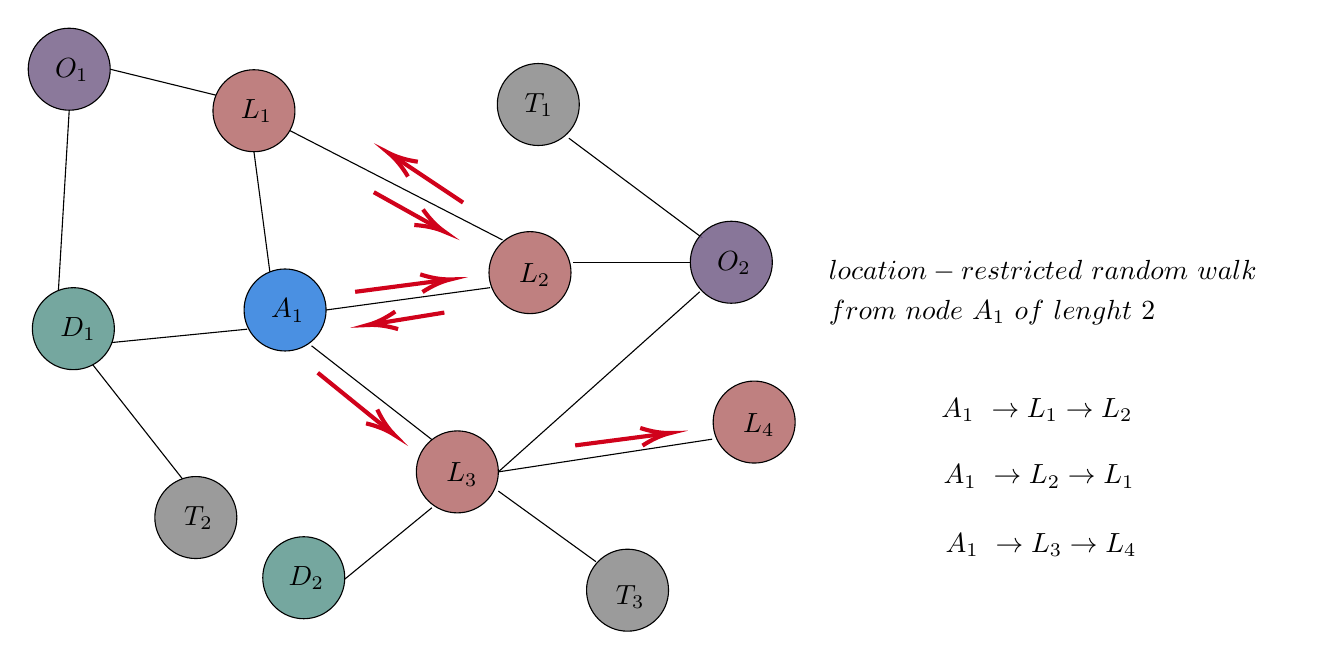
\begin{tikzpicture}[x=0.75pt,y=0.75pt,yscale=-1,xscale=1]
%uncomment if require: \path (0,424); %set diagram left start at 0, and has height of 424

%Shape: Circle [id:dp7408051866775183] 
\draw  [fill={rgb, 255:red, 120; green, 99; blue, 139 }  ,fill opacity=0.86 ] (25,44.75) .. controls (25,33.84) and (33.84,25) .. (44.75,25) .. controls (55.66,25) and (64.5,33.84) .. (64.5,44.75) .. controls (64.5,55.66) and (55.66,64.5) .. (44.75,64.5) .. controls (33.84,64.5) and (25,55.66) .. (25,44.75) -- cycle ;
%Straight Lines [id:da23542430963110572] 
\draw    (285.5,78) -- (349.75,126) ;


%Straight Lines [id:da9464008253728087] 
\draw    (64.5,44.75) -- (118.5,58) ;


%Straight Lines [id:da08217413408429564] 
\draw    (133.75,84.5) -- (141.5,143) ;


%Straight Lines [id:da09323667666851287] 
\draw    (130.5,170) -- (59.5,177) ;


%Straight Lines [id:da7962118124877697] 
\draw    (56,187) -- (105.5,250) ;


%Straight Lines [id:da5871309233503423] 
\draw    (161.5,178) -- (220.5,224) ;


%Straight Lines [id:da34174484678938555] 
\draw    (253.5,127) -- (148.5,73) ;


%Straight Lines [id:da666737517633426] 
\draw    (39.5,152) -- (44.75,64.5) ;


%Shape: Circle [id:dp2508008248936129] 
\draw  [fill={rgb, 255:red, 117; green, 167; blue, 159 }  ,fill opacity=1 ] (27,169.75) .. controls (27,158.84) and (35.84,150) .. (46.75,150) .. controls (57.66,150) and (66.5,158.84) .. (66.5,169.75) .. controls (66.5,180.66) and (57.66,189.5) .. (46.75,189.5) .. controls (35.84,189.5) and (27,180.66) .. (27,169.75) -- cycle ;
%Shape: Circle [id:dp4060574393112093] 
\draw  [fill={rgb, 255:red, 191; green, 128; blue, 128 }  ,fill opacity=1 ] (114,64.75) .. controls (114,53.84) and (122.84,45) .. (133.75,45) .. controls (144.66,45) and (153.5,53.84) .. (153.5,64.75) .. controls (153.5,75.66) and (144.66,84.5) .. (133.75,84.5) .. controls (122.84,84.5) and (114,75.66) .. (114,64.75) -- cycle ;
%Shape: Circle [id:dp36486264653360756] 
\draw  [fill={rgb, 255:red, 74; green, 144; blue, 226 }  ,fill opacity=1 ] (129,160.75) .. controls (129,149.84) and (137.84,141) .. (148.75,141) .. controls (159.66,141) and (168.5,149.84) .. (168.5,160.75) .. controls (168.5,171.66) and (159.66,180.5) .. (148.75,180.5) .. controls (137.84,180.5) and (129,171.66) .. (129,160.75) -- cycle ;
%Shape: Circle [id:dp08674187749849449] 
\draw  [fill={rgb, 255:red, 155; green, 155; blue, 155 }  ,fill opacity=1 ] (86,260.75) .. controls (86,249.84) and (94.84,241) .. (105.75,241) .. controls (116.66,241) and (125.5,249.84) .. (125.5,260.75) .. controls (125.5,271.66) and (116.66,280.5) .. (105.75,280.5) .. controls (94.84,280.5) and (86,271.66) .. (86,260.75) -- cycle ;
%Shape: Circle [id:dp8835082221714545] 
\draw  [fill={rgb, 255:red, 155; green, 155; blue, 155 }  ,fill opacity=1 ] (251,61.75) .. controls (251,50.84) and (259.84,42) .. (270.75,42) .. controls (281.66,42) and (290.5,50.84) .. (290.5,61.75) .. controls (290.5,72.66) and (281.66,81.5) .. (270.75,81.5) .. controls (259.84,81.5) and (251,72.66) .. (251,61.75) -- cycle ;
%Shape: Circle [id:dp7841302136434047] 
\draw  [fill={rgb, 255:red, 191; green, 128; blue, 128 }  ,fill opacity=1 ] (212,238.75) .. controls (212,227.84) and (220.84,219) .. (231.75,219) .. controls (242.66,219) and (251.5,227.84) .. (251.5,238.75) .. controls (251.5,249.66) and (242.66,258.5) .. (231.75,258.5) .. controls (220.84,258.5) and (212,249.66) .. (212,238.75) -- cycle ;
%Shape: Circle [id:dp12337615634170196] 
\draw  [fill={rgb, 255:red, 120; green, 99; blue, 139 }  ,fill opacity=0.88 ] (344,137.75) .. controls (344,126.84) and (352.84,118) .. (363.75,118) .. controls (374.66,118) and (383.5,126.84) .. (383.5,137.75) .. controls (383.5,148.66) and (374.66,157.5) .. (363.75,157.5) .. controls (352.84,157.5) and (344,148.66) .. (344,137.75) -- cycle ;
%Straight Lines [id:da5234252867958065] 
\draw    (247.5,150) -- (168.5,160.75) ;


%Shape: Circle [id:dp4211477572325999] 
\draw  [fill={rgb, 255:red, 191; green, 128; blue, 128 }  ,fill opacity=1 ] (247,142.75) .. controls (247,131.84) and (255.84,123) .. (266.75,123) .. controls (277.66,123) and (286.5,131.84) .. (286.5,142.75) .. controls (286.5,153.66) and (277.66,162.5) .. (266.75,162.5) .. controls (255.84,162.5) and (247,153.66) .. (247,142.75) -- cycle ;
%Shape: Circle [id:dp9232049858802234] 
\draw  [fill={rgb, 255:red, 191; green, 128; blue, 128 }  ,fill opacity=1 ] (355,214.75) .. controls (355,203.84) and (363.84,195) .. (374.75,195) .. controls (385.66,195) and (394.5,203.84) .. (394.5,214.75) .. controls (394.5,225.66) and (385.66,234.5) .. (374.75,234.5) .. controls (363.84,234.5) and (355,225.66) .. (355,214.75) -- cycle ;
%Straight Lines [id:da08982203790987131] 
\draw    (348.5,152) -- (251.5,238.75) ;


%Straight Lines [id:da4146904879227602] 
\draw    (251.5,248) -- (298.5,282) ;


%Shape: Circle [id:dp7153221143722261] 
\draw  [fill={rgb, 255:red, 155; green, 155; blue, 155 }  ,fill opacity=1 ] (294,295.75) .. controls (294,284.84) and (302.84,276) .. (313.75,276) .. controls (324.66,276) and (333.5,284.84) .. (333.5,295.75) .. controls (333.5,306.66) and (324.66,315.5) .. (313.75,315.5) .. controls (302.84,315.5) and (294,306.66) .. (294,295.75) -- cycle ;
%Straight Lines [id:da3306416978098605] 
\draw    (344,137.75) -- (287.5,137.75) ;


%Straight Lines [id:da16914689456540688] 
\draw    (251.5,238.75) -- (354.5,223) ;


%Straight Lines [id:da8196413178699977] 
\draw    (219.5,256) -- (169.5,297) ;


%Shape: Circle [id:dp7363989977901311] 
\draw  [fill={rgb, 255:red, 117; green, 167; blue, 159 }  ,fill opacity=1 ] (138,289.75) .. controls (138,278.84) and (146.84,270) .. (157.75,270) .. controls (168.66,270) and (177.5,278.84) .. (177.5,289.75) .. controls (177.5,300.66) and (168.66,309.5) .. (157.75,309.5) .. controls (146.84,309.5) and (138,300.66) .. (138,289.75) -- cycle ;
%Straight Lines [id:da46101722896412034] 
\draw [color={rgb, 255:red, 208; green, 2; blue, 27 }  ,draw opacity=1 ][line width=1.5]    (164.5,191) -- (199.17,219.11) ;
\draw [shift={(201.5,221)}, rotate = 219.04] [color={rgb, 255:red, 208; green, 2; blue, 27 }  ,draw opacity=1 ][line width=1.5]    (14.21,-4.28) .. controls (9.04,-1.82) and (4.3,-0.39) .. (0,0) .. controls (4.3,0.39) and (9.04,1.82) .. (14.21,4.28)   ;

%Straight Lines [id:da0015886548375136922] 
\draw [color={rgb, 255:red, 208; green, 2; blue, 27 }  ,draw opacity=1 ][line width=1.5]    (288.5,226) -- (331.53,220.39) ;
\draw [shift={(334.5,220)}, rotate = 532.5699999999999] [color={rgb, 255:red, 208; green, 2; blue, 27 }  ,draw opacity=1 ][line width=1.5]    (14.21,-4.28) .. controls (9.04,-1.82) and (4.3,-0.39) .. (0,0) .. controls (4.3,0.39) and (9.04,1.82) .. (14.21,4.28)   ;

%Straight Lines [id:da793413521169541] 
\draw [color={rgb, 255:red, 208; green, 2; blue, 27 }  ,draw opacity=1 ][line width=1.5]    (182.5,152) -- (225.53,146.39) ;
\draw [shift={(228.5,146)}, rotate = 532.5699999999999] [color={rgb, 255:red, 208; green, 2; blue, 27 }  ,draw opacity=1 ][line width=1.5]    (14.21,-4.28) .. controls (9.04,-1.82) and (4.3,-0.39) .. (0,0) .. controls (4.3,0.39) and (9.04,1.82) .. (14.21,4.28)   ;

%Straight Lines [id:da605573841249404] 
\draw [color={rgb, 255:red, 208; green, 2; blue, 27 }  ,draw opacity=1 ][line width=1.5]    (234.5,109) -- (201,86.66) ;
\draw [shift={(198.5,85)}, rotate = 393.69] [color={rgb, 255:red, 208; green, 2; blue, 27 }  ,draw opacity=1 ][line width=1.5]    (14.21,-4.28) .. controls (9.04,-1.82) and (4.3,-0.39) .. (0,0) .. controls (4.3,0.39) and (9.04,1.82) .. (14.21,4.28)   ;

%Straight Lines [id:da8984952940487898] 
\draw [color={rgb, 255:red, 208; green, 2; blue, 27 }  ,draw opacity=1 ][line width=1.5]    (191.5,104) -- (222.88,121.54) ;
\draw [shift={(225.5,123)}, rotate = 209.2] [color={rgb, 255:red, 208; green, 2; blue, 27 }  ,draw opacity=1 ][line width=1.5]    (14.21,-4.28) .. controls (9.04,-1.82) and (4.3,-0.39) .. (0,0) .. controls (4.3,0.39) and (9.04,1.82) .. (14.21,4.28)   ;

%Straight Lines [id:da28022849120737825] 
\draw [color={rgb, 255:red, 208; green, 2; blue, 27 }  ,draw opacity=1 ][line width=1.5]    (225.5,162) -- (191.46,167.52) ;
\draw [shift={(188.5,168)}, rotate = 350.78999999999996] [color={rgb, 255:red, 208; green, 2; blue, 27 }  ,draw opacity=1 ][line width=1.5]    (14.21,-4.28) .. controls (9.04,-1.82) and (4.3,-0.39) .. (0,0) .. controls (4.3,0.39) and (9.04,1.82) .. (14.21,4.28)   ;


% Text Node
\draw (46,45) node   {$O_{1}$};
% Text Node
\draw (49,170) node   {$D_{1}$};
% Text Node
\draw (135,65) node   {$L_{1}$};
% Text Node
\draw (150,161) node   {$A_{1}$};
% Text Node
\draw (107,261) node   {$T_{2}$};
% Text Node
\draw (271,62) node   {$T_{1}$};
% Text Node
\draw (234,240) node   {$L_{3}$};
% Text Node
\draw (365,138) node   {$O_{2}$};
% Text Node
\draw (269,144) node   {$L_{2}$};
% Text Node
\draw (377,216) node   {$L_{4}$};
% Text Node
\draw (315,299) node   {$T_{3}$};
% Text Node
\draw (159,290) node   {$D_{2}$};
% Text Node
\draw (516,152) node   {$ \begin{array}{l}
location-restricted\ random\ walk\ \\
from\ node\ A_{1} \ of\ lenght\ 2\ 
\end{array}$};
% Text Node
\draw (511,209) node   {$A_{1} \ \rightarrow L_{1} \rightarrow L_{2}$};
% Text Node
\draw (512,241) node   {$A_{1} \ \rightarrow L_{2} \rightarrow L_{1}$};
% Text Node
\draw (513,274) node   {$A_{1} \ \rightarrow L_{3} \rightarrow L_{4}$};


\end{tikzpicture}

}
\caption{An example of type restricted random walk of length $2$ for node types location and starting node $A_1$.}
\label{fig:facetteddeepwalk}
\end{figure} 
 %%%%%%%%%%%%%%%%%%%%%%%%%%%%%%%%%%%%%%%%%%%%%%%%%%%%%%%%%%%%
\section{Similarity Between Embeddings}
In the previous chapter, we presented cosine similarity as the main similarity measure between word vectors. To take advantage of the separation in dimensions for faceted embedding, an additional vector multiplication for cosine similarity is defined, resulting into two types of similarity:  
\begin{itemize}
\item \emph{Full similarity:} Using the full dimensions of the vectors for computing the cosine similarity or dot product between them, indicating that the full embedding vector, containing a concatenation of all types. 
\item \emph{Partial similarity:} Using dimensions based on the query words. For example, if the similarity between an actor and a term is requested, only dimensions related to actors and terms in both embeddings were kept to compute the cosine similarity. This method was used to test whether the particular dimensions keep the most informative information about a type or not. Partial similarity can also be viewed as looking at the similarity between two word vectors in a chosen dimension. For example, looking only at cosine similarity between the organisation part of two embeddings will show how close they are in the organisation subspace. 
\end{itemize}


 %%%%%%%%%%%%%%%%%%%%%%%%%%%%%%%%%%%%%%%%%%%%%%%%%%%%%%%%%%%%
\section{Summary}\label{sec:faceted_summary}
In this chapter, we introduced three models for learning faceted embeddings with separable components, where each component defines the relation of a word to entities of a specific type. We modified the existing word embedding and graph embedding techniques to achieve a more flexible definition of context for a word, where for each component the context is limited to entities of a certain type. As input for all models, we used the co-occurrence graph extracted on annotated text, which contains the entity-entity relations and captures their co-occurrence with terms. From the word embedding methods, we modify GloVe and word2vec and from the graph-embedding models, we chose DeepWalk with type-restricted random walks. In Chapter~\ref{chap:eval}, we evaluate the faceted models against the well-established word embedding methods on various evaluation tasks and discuss their advantages and drawbacks.


  %%%%%%%%%%%%%%%%%%%%%%%%%%%%%%%%%%%%%%%%%%%%%%%%%%%%%%%%%%%%
\chapter{Experimental Evaluation}
\label{chap:eval}
In this chapter, we present different methods of evaluation for entity embeddings and the faceted models. In Section~\ref{sec:eval_embeddings}, most common methods for evaluation of word embeddings are discussed and the ones chosen for this study are presented. Section~\ref{sec:data} explains the dataset used for training the embeddings, the preprocessing and graph extraction. Evaluation setup and parameter tuning for the models is discussed in Section~\ref{sec:setup}. Evaluation results for the common tasks are shown in Section~\ref{sec:eval_results}, where the results for the entity embeddings and faceted models are discussed separately in Subsections~\ref{subsec:eval_entity} and \ref{subsec:eval_faceted} respectively. Finally, Section~\ref{sec:eval_experimental} contains the experimental exploration and visualization of the embeddings neighbourhood. 
%%%%%%%%%%%%%%%%%%%%%%%%%%%%%%%%%%%%%%%%%%%%%%%%%%%%%%%%%%%%
\section{Evaluation of Word Embeddings}\label{sec:eval_embeddings}
In general, the evaluation of word embeddings falls into two major categories: The extrinsic and intrinsic evaluation. In an extrinsic evaluation, trained embeddings are used as input of some downstream task and the performance is measured by a metric specific to that task. Example of downstream tasks for embeddings are POS tagging~\brackettext{\cite{DBLP:conf/naacl/LingDBT15}}, named entity recognition~\brackettext{\cite{DBLP:conf/sdm/Al-RfouKPS15}}, and dependency parsing~\brackettext{\cite{DBLP:conf/emnlp/ChenM14}}. However, since evaluations are task-specific, an embedding that works well for one task may fail for another. The more popular evaluation technique for word embedding is intrinsic evaluation, which  directly tests for syntactic or semantic relationships between words. These tasks analyze how well the embeddings capture certain syntactic or semantic relations between a set of query and target words, referred to as \textit{query inventory}~\brackettext{\cite{DBLP:conf/emnlp/SchnabelLMJ15}}. Intrinsic tasks are easier and faster to test and provide a quick understanding of the system. The main drawback of intrinsic evaluation is that the notion of semantics is not universal~\brackettext{\cite{DBLP:journals/corr/abs-1801-09536}}. Some datasets reflect semantic relatedness and some semantic similarity, while very similar they measure quite different attributes. Two words are considered semantically similar if they are synonymous and can be substituted for each other in context. For instance, \emph{``rose''} and \emph{``flower''}. Semantic relatedness, however, is a broader concept. Words with any functional associations, like belonging to the same semantic field, are considered semantically related, e.g., \emph{``rose''} and \emph{``thorn''}~\brackettext{\cite{DBLP:conf/nodalida/Kolb09}}. It is not obvious if the word embeddings should favor relatedness over similarity or vice versa. Furthermore, a high accuracy on these tasks does not necessarily mean that the model will perform well on real tasks unless some correlation between them is established. Thus, testing the model on an intrinsic task at first and an extrinsic task in final steps can provide a better overview of the model performance. Since there are no entity-centric extrinsic evaluation tasks in the literature and few intrinsic datasets include entities, we focus on the performance in term-based intrinsic tasks. We create some of our own datasets to incorporate the entities, but it is important to emphasize that the true potential of these entity-based models can only be investigated in the presence of suitable evaluation datasets. Following the approach by~\brackettext{\cite{DBLP:conf/emnlp/SchnabelLMJ15}}, we use three kinds of intrinsic evaluations. In the following, we describe each task and give a brief description of the datasets we use for evaluating each of them. 
%%%%%%%%%%%%%%%%%%%%%%%%%%%%%%%%%%%%%%%%%%%%%%%%%%%%%%%%%%%%
 \subsection{Relatedness}
This task is based on datasets containing relatedness or similarity scores for pairs of words annotated by humans; the cosine similarity or Euclidean distance between the embeddings for two words should have high correlation (Spearman or Pearson) with human similarity or relatedness scores. We choose seven datasets containing both relatedness and similarity scores. 
\begin{enumerate}
 \item \emph{Similarity353:} $203$ instances of similar word pairs from WordSim353~\brackettext{\cite{DBLP:conf/naacl/AgirreAHKPS09}}. Scores scale from 0 (totally unrelated words) to 10 (very much related or identical words). Word pairs are classified as synonyms, antonyms, or identical, and unrelated pairs (pairs with average similarity less than or equal to $5$)~\brackettext{\cite{DBLP:conf/naacl/AgirreAHKPS09}}.
 \item \emph{Relatedness353:} $252$ instances of word pairs from WordSim353~\brackettext{\cite{DBLP:conf/naacl/AgirreAHKPS09}} that are not similar (are not present in the Similarity353 subset), but are still considered related by humans with an average similarity greater than $5$, and unrelated pairs~\brackettext{\cite{DBLP:conf/naacl/AgirreAHKPS09}}.
 \item \emph{MEN:} $3,000$ word pairs with human-assigned similarity judgments, which instead of an absolute score is based on comparative judgments on two pair exemplars at a time. Each person was given a binary choice of \emph{``right''} or \emph{``wrong''} and in total each pair was compared $50$ times, thus obtaining a final score on a $50$ point scale~\brackettext{\cite{DBLP:journals/jair/BruniTB14}}.
 \item \emph{RG65:} $65$ pairs with annotated similarity scaling from $0$ to $4$, where the similarity between two words is measured by the similarity of their meaning and the amount of overlap for each definition of context~\brackettext{\cite{DBLP:journals/cacm/RubensteinG65}}.
 \item \emph{RareWord:} $2,034$ rare word pairs with human similarity scores. For creating the dataset they select a list of rare words and for each find another word (not necessarily rare) to form a pair and assess human judgments on how similar each pair is on a scale of $0$ to $10$~\brackettext{\cite{DBLP:conf/conll/LuongSM13}}.
 \item \emph{SimLex-999:} $999$ pairs of human-labeled examples of semantic relatedness, containing a selection of adjective, verb, and noun concept pairs. The scores range from $0$ to $10$~\brackettext{\cite{DBLP:journals/coling/HillRK15}}.
 \item \emph{MTurk:} $771$ word pairs with semantic relatedness scores from
$0$ to $5$, where scores were collected on Amazon Mechanical Turk~\brackettext{\cite{DBLP:conf/www/RadinskyAGM11}}.
\end{enumerate}
Similarity between the word pairs is typically computed by the cosine similarity of their respective word vectors. In the case of faceted models, we can investigate the similarity between two words further by looking at separate components. For this purpose, we take advantage of the partial similarity defined in Chapter~\ref{chap:faceted} and compute the correlation between human annotations and partial similarity of each component separately. In addition, assuming that most of the information about the relationship between the two words is in the component corresponding to their types, we compute the similarity between the types in relation. For example, if two words are of types actor and term, the actor and term component of the in both embeddings are kept and the cosine similarity is computed based on the two component related to word types in question. 
%%%%%%%%%%%%%%%%%%%%%%%%%%%%%%%%%%%%%%%%%%%%%%%%%%%%%%%%%%%%
\subsection{Analogy}
This task was popularized by the word2vec paper~\brackettext{\cite{DBLP:journals/corr/abs-1301-3781}}, where the goal is to find a term $x$ for a given term $y$, such that  $x : y$ best resembles a sample relationship $a : b$. In other words, given the triple $(a,b,x)$, the aim is to find the target word $y$ correctly. To find the target word we do the following:  
\begin{itemize}
    \item Compute $w_a-w_b=w_{a-b}$, where $w_a$ and $w_b$ are the embeddings for word $a$ and $b$. 
    \item Compute the mean vector $w_{mean}=w_{a-b}+w_x$.
    \item Find the nearest neighbour to $w_{mean}$ (the one with the highest cosine similarity) if it is $w_y$, the analogy was found correctly.
  \end{itemize}
  \noindent
For entity embeddings, where the type of the embedding is known, we can also consider an easier, type-specific variation of this task, which only considers neighbours that match a given entity class. In the type-specific variation we only consider candidates that have the same entity type as the words in the triple $(a,b,x)$, thus making the task easier. We use two dataset for evaluating this task: 
\begin{enumerate}
 \item \emph{GA}: The \emph{Google Analogy} data consists of $19,544$ pairs ($8,869$ semantic and $10,675$ syntactic), with $14$ types of relations ($9$ morphological and $5$ semantic), used in the word2vec paper~\brackettext{\cite{DBLP:journals/corr/abs-1301-3781}}. Beyond terms, it contains some location entities of cities and countries. The types and their meaning are shown in Table~\ref{table:analogy_types}.
\item \emph{MSR:} The \emph{Microsoft Research Syntactic analogies} dataset contains $8,000$ morphological questions. The questions contain base/comparative/superlative forms of adjectives; singular/plural forms of common nouns; possessive/non-possessive forms of common nouns; and base, past and 3rd person present tense forms of verbs~\cite{DBLP:conf/naacl/MikolovYZ13}. All word pairs in this dataset are terms.
\end{enumerate}


\begin{table}[h]
\centering

\begin{tabular}{ll}
        \toprule
{Morphological} & \\         \midrule

gram1-adjective-to-adverb:& an adverb with its adjective.            \\ \hline
gram2-opposite: &noun and its opposite.                          \\ \hline
gram3-comparative: & an adjective with its comparative.                                           \\ \hline
gram4-superlative:&an adjective with its superlative.                                                    \\ \hline
gram5-present-participle:&participles and their verb in infinitive.                                           \\ \hline
gram6-nationality-adjective:&country with its nationality.                                                                \\ \hline
gram7-past-tense: &verbs in infinitive and past form.                                                             \\ \hline
gram8-plural:& nouns in single and plural from.                                                         \\ \hline
gram9-plural-verbs: &verbs in singular and plural.                                                          \\ 
\midrule
\midrule
{Semantic}&\\   
\midrule

capital-common-countries:                 &           selection of countries and their capitals.\\ \hline
capital-world:          &        all countries and their capitals.    \\ \hline
family:     &             family relations such as brother and sister  \\ \hline
city-in-state:   &      states and their cities name (US). \\ \hline
currency:    &        name of a country with its currency.  \\
\bottomrule
\end{tabular}
 \caption{Types of questions in the Google Analogy test, in total nine
  morphological and five semantic questions.} 
  \label{table:analogy_types}
\end{table}
%%%%%%%%%%%%%%%%%%%%%%%%%%%%%%%%%%%%%%%%%%%%%%%%%%%%%%%%%%%%
\subsection{Categorization}
When projecting the word embedding in a 2 or 3-dimensional space, we expected that the similar words form meaningful clusters. The embedding can be projected using \emph{t-SNE}~\brackettext{\cite{SCHOL:journals/jmlr/Maaten}} or PCA. Vectors of all words are either visualised for exploratory analysis or clustered using a clustering algorithm of choice and the purity of the returned clusters is computed as a metric for this task~\brackettext{\cite{DBLP:books/daglib/0021593}}. For evaluating the embeddings on categorization task, we use two datasets from the Lexical Semantics Workshop, which do not contain entities. Additionally, we created three test sets using \emph{Wikidata Query Service} to find entities of type person, location, and organization. In each case, up to $30$ entities form each category were chosen based on the highest frequency in our training data.
\begin{enumerate}
  \item \emph{ESSLLI\_1a:} Acronym for the European Summer School in Logic, Language
and Information. The goal of the task is to group concrete nouns into semantic categories and contains $44$ concrete nouns that belong to six semantic categories~\brackettext{\cite{SCHO:workshop/Baroni}}. 
  \item \emph{ESSLLI\_2c:} The goal of the sub-task is to group verbs into semantic categories and contains$45$ verbs that belong to nine semantic classes~\brackettext{\cite{SCHO:workshop/Baroni}}.
  \item \emph{Cities:} $150$ major cities in the U.S., the U.K., and Germany. 
  \item \emph{Politicians:} $150$ politicians from the U.S., the U.K., and Germany.
  \item \emph{Companies:} $110$ software companies, Web services, and car manufacturers. 
\end{enumerate}
%%%%%%%%%%%%%%%%%%%%%%%%%%%%%%%%%%%%%%%%%%%%%%%%%%%%%%%%%%%%
\section{Training Data}\label{sec:data}
For training, we use $209,023$ news articles from English-speaking news outlets, collected from June to November $2016$~\brackettext{\cite{DBLP:conf/ecir/SpitzG18}}. The data contains a total of $5,427,383$ sentences and $4,468,993$ tokens. To train the regular word embeddings, we use the raw article text, with only common preprocessing steps. The pre-processing steps contain tokenization of all articles into words and removal of stop words and punctuations. Non-alphabetic characters, like Chinese or Arabic vocabulary, are disregard and multiple white spaces are reduced to only one. Any HTML tags or numeric values are also removed from the text, to produce a clean document, containing only terms relevant to the model. In addition, all the words are converted to their lower-case form to avoid multiple representations of a single term.\\
For annotated embeddings, prior to named entity annotation, POS tagging is performed by the Stanford POS tagger~\brackettext{\cite{DBLP:conf/naacl/ToutanovaKMS03}}. 
We removed punctuation and stop-word and filtered terms in the text to a certain POS-tag. Unnecessary tags are removed, namely  wh-determiner, wh-pronouns, wh-adverbs, common verbs, such as \emph{have} and \emph{do} in past or present, interjections (e.g. ah!, dear me!) and other terms that mostly fall into stop-words category such as: predeterminer (both and a lot of), possessive endings, prepositions (until, before,\dots), determiner (a, the, every) and coordinating conjunction (and, but, or). Afterwards, we extract named entities with \emph{Ambiverse}\footnote{\url{https://www.ambiverse.com}}, a state-of-the-art commercial annotator that links entity mentions to Wikidata identifiers and select named entities that correspond to persons, locations, and organizations. For temporal expressions (date entities) we use \emph{HeidelTime}~\brackettext{\cite{DBLP:journals/lre/StrotgenG13}}.\\
To generate input for the graph-based embeddings, we extract an implicit graph of locations, organizations, persons (actors), dates, and terms, using the extraction code of the LOAD model~\brackettext{\cite{DBLP:conf/sigir/SpitzG16}}. In the LOAD model, we include term co-occurrences only inside sentences and entity-entity co-occurrences up to a default window size of five sentences, thus, there exists an edge between terms and other words only if they appear in the same sentence. The generated graph contains $T=93,390$ nodes and $E=9,584,191$ edges. From which $D=2,442$  are date entities, $L=4,659$ location, $A=10,537$ actors, $O=3,789$ organisations and $T=71,963$ are terms. Since the evaluation datasets contain words that are not present in the training vocabulary, each data set is filtered accordingly.
%%%%%%%%%%%%%%%%%%%%%%%%%%%%%%%%%%%%%%%%%%%%%%%%%%%%%%%%%%%%
\section{Parameter Tuning } \label{sec:setup}
To achieve best performance we perform extensive parameter tuning for each model and only report the results for the best one. To make the embeddings comparable, all embeddings have $100$ dimensions. In the following, we first discuss the best parameter settings for annotated and raw models and then for faceted embeddings. Because of the random initialization of at the beginning of the training, all entity and raw models are trained $10$ times and the average performance is reported. Nevertheless, since faceted models were only an extension to annotated models and are only trained for experimental analysis we trained a single model for each. For all the models, instead of a typical grid search, we chose a coarse-to-fine method, where instead of checking all the possible combinations, we randomly sampled some parameters and focused on the areas, where better models are trained.
 %%%%%%%%%%%%%%%%%%%%%%%%%%%%%%%%%%%%%%%%%%%%%%%%%%%%%%%%%%%%
\subsection{Parameter setting for entity embeddings and regular word embeddings}
 
\emph{Word2vec-based models} both the word2vec on the raw data ($r$W2V) and on the annotated corpus ($a$W2V) are trained with a learning rate of $0.015$ and a window size of $10$. We use $8$ negative samples on the raw data, and $16$ on the annotated data. In addition to data pre-processing, we removed words with a frequency of less than $3$, as there is not enough data to learn a meaningful representation of them. \\

\noindent
\emph{GloVe-based models}, namely GloVe model on the raw data ($r$GLV) and on the annotated text ($a$GLV) are trained with a learning rate of $0.06$ and a window size of $10$. For the weighting function, we did not use the authors suggested values, instead performed additional parameter tuning, which resulted to a scaling factor of $0.5$ and a maximum cut-off of $1000$ to obtain best performance. Words that occur less than $5$ times are removed from the input.\\

\noindent
\emph{DeepWalk models} use $100$ random walks of length $4$ from each node, for both identity (DW$_{id}$) and logarithmic (DW$_{log}$) mapping. We did not experiment with walk lengths larger than $5$, because the co-occurrence graph is dense and has a relatively small diameter. Thus, longer walks would introduce unrelated words into contexts and reduce the performance. For the skip-gram model, which was trained on the random walk corpus, we use a learning rate of $0.015$ and $64$ negative samples with the window-size of $10$. We removed words that were visited less than $3$ times in the random walk corpus. \\

\noindent
\emph{VERSE models} have relatively small parameters for tuning. We use a learning rate of $0.025$ and $16$ negative samples.\\

\noindent
Because of different inputs for each embedding model, comparison between them is not trivial. One main challenge is the fact that the training process of graph-based and textual methods is essentially incomparable. Graph-based models do not have a textual corpus and require an additional step of creating something similar either with a random walk or node sampling. Typically, the performance of neural network based models increases with the number of iterations and more data. While the textual models consider one pass through the corpus as one iteration, an iteration for the graph-based model is a different concept and not the only factor for increasing performance. The data size in graph-based models is not limited to the corpus but the sampling process. The number of random walks that is used in DeepWalk corresponds directly to the performance, the more random walk, the larger the corpus and better the performance of the skip-gram model trained on it, even if the number of iterations is fixed. On the other hand, increasing the number of random walks also increases the runtime. In contrast, the VERSE model has no notion of iteration and samples nodes for positive observations from the empirical similarity distribution and negative observations from a noise distribution. The more samples, better the performance, and longer the runtime. Thus, to approach a fair evaluation, we use similar training times for all models (roughly $10$ hours per model on a $100$ core machine). We fix the number of iterations of the textual models and DeepWalk's skip-gram at $100$. For VERSE, we use $50,000$ sampling steps to obtain a comparable runtime.
%%%%%%%%%%%%%%%%%%%%%%%%%%%%%%%%%%%%%%%%%%%%%%%%%%%%%%%%%%%%
\subsection{Parameter setting for faceted models}
\emph{Faceted GloVe model} is trained with a learning rate of $0.05$. For best performance, we use focal addition and weighing function. The scaling factor for the weighting function is set to $0.75$ and maximum cut-off of $1000$ is used. All nodes with less than $5$ edges are removed from the training data, before generating the weighted adjacency matrix. Normalization and adding $1$ to the logarithm are disregard as they did not improve the results. Moreover, we only report the results for $f$GLV$_{sep}$, which refers to the separate cost function as the performance of both cost functions are similar. To achieve the faceted components, each component is trained separately with the same parameter setting and embedding size of $20$, which after concatenation creates the full $100$ dimensional embeddings. \\

\noindent
\emph{Faceted word2vec model} is trained with the learning rate of $0.015$ and $32$ negative sample. To achieve the embedding size of $100$, each component has the embeddings size of $20$. Any words that have less than $3$ edges in the co-occurrence graph are removed. \\

\noindent
\emph{Faceted DeepWalk models} use $100$ random walks of length $4$ from each node. We train the embeddings once using logarithmic normalization ($f$DW$_{log}$) and once without any normalization ($f$DW$_{id}$). The skip-gram models uses a learning rate of $0.015$ and $32$ negative samples. The window size is set to $10$ and any node that is visited less than $3$ times in the random walk corpus is removed from the models. 

%%%%%%%%%%%%%%%%%%%%%%%%%%%%%%%%%%%%%%%%%%%%%%%%%%%%%%%%%%%%
\section{Evaluation Results}\label{sec:eval_results}
In the following, we discuss the results for relatedness, analogy and clustering tasks for entity embeddings and faceted models separately. We compare our approaches against the word embeddings trained on raw text and analysis their weaknesses and strength. For the faceted models, we take advantage of the separable dimensions and in addition to testing the embeddings in their full dimension, we also look at components separately. The results for faceted GloVe model is not presented on all tasks, because of an extreme lack of performance. 
%%%%%%%%%%%%%%%%%%%%%%%%%%%%%%%%%%%%%%%%%%%%%%%%%%%%%%%%%%%%
\subsection{Evaluation of entity embeddings}\label{subsec:eval_entity}
The results of the relatedness task for entity embeddings are shown in Table~\ref{wordsim_normal}. On this data, word2vec model predominantly performs better than GloVe on both raw and annotated text. Nevertheless, the performance of both models degrades slightly after annotation. 
Therefore, to create embeddings of entities naively using a word embedding method on an annotated corpus results into a loss in performance. However, since all datasets consist mostly of terms, this deduction cannot be extended to entity-centric evaluations. The DeepWalk-based models perform better than GloVe, but do poorly overall. The logarithmic normalization boosts the performance of the DeepWalk-based model slightly but not enough to compete with word2vec. Results for the VERSE model are rather diverse, in a sense that it works very well on some tasks, but is worse than word2vec trained on the raw data for rare words and the SimLex dataset. This is likely caused by the conceptual structure of the co-occurrence graph on which VERSE is trained, which captures relatedness and not similarity as tested by SimLex. Whereas on datasets, such as Relatedness353 and MEN, which are designed for relatedness tasks, VERSE is clearly the better choice. On average, word2vec based models outperform the rest on similarity tasks, both the model trained on raw text and on the annotated data have the highest scores on average. Thus, we can conclude that for purely term-based tasks, word2vec is the best choice for measuring word similarity, while VERSE captures the relatedness better. 

\begin{table}[t]
\caption{Word similarity results. Shown are the Pearson correlations between the cosine similarity of the embeddings and the human score on the word similarity datasets. The two best values per task are highlighted.}
\label{wordsim_normal}
\setlength{\tabcolsep}{6pt} % Default value: 6pt
\renewcommand{\arraystretch}{1.0} % Default value: 1
\resizebox{\textwidth}{!}{%
\begin{tabular}{lcccccccc}

\toprule
 & $r$W2V & $r$GLV & $a$W2V & $a$GLV & DW$_{id}$ & DW$_{log}$ & VRS \\
\midrule
%Wordsim353         & \textbf{0.586}   & 0.413   & 0.585& 0.412& 0.530  & 0.533     & \textbf{0.599}\\ %all of WordSim353
Similarity353      &   \boldmath $\num{ 0.700}$   & 0.497   &   \boldmath $\num{ 0.697}$ & 0.450 & 0.571  & 0.572     & 0.641\\
Relatedness353     &   \boldmath $\num{0.509}$   & 0.430   & 0.507& 0.428& 0.502  & 0.506   & \boldmath $\num{0.608}$\\
MEN                &\boldmath $\num{0.619}$   & 0.471   & \boldmath $\num{0.619}$& 0.469& 0.539  & 0.546     & \boldmath $\num{0.640}$\\ 
RG65               & \boldmath $\num{0.477}$   & 0.399   & 0.476& 0.386& 0.312  & 0.344     & \boldmath $\num{0.484}$\\ 
RareWord           & \boldmath $\num{0.409}$   & 0.276   & \boldmath $\num{0.409}$& 0.274& \boldmath $\num{0.279}$  & 0.276    & 0.205\\  
SimLex-999         &\boldmath $\num{0.319}$   & 0.211   & \boldmath $\num{0.319}$ & 0.211& \boldmath $\num{0.279}$  & 0.201      & 0.236\\ 
MTurk              & \boldmath $\num{0.647}$  & 0.493   & 0.644& 0.502& 0.592  & 0.591   & \boldmath $\num{0.687}$\\
\midrule
average            & \boldmath $\num{0.526}$   & 0.400   & \boldmath $\num{0.524}$ & 0.389 & 0.439  & 0.433   & 0.500 \\
\bottomrule
\end{tabular}%
}
%\vspace*{-10pt}
\end{table}
% comparison on locations in GA data set:
% total locations = 6892
% correct VRS = 1662 = 24.1%
% correct aW2V = 14 = 0.20%
% correct aGLV = 16 = 0.23%

Table~\ref{analogy_normal} shows the accuracy achieved by entity-based and term-based models in the words analogy task. The overall results are quite poor for all models, which we attribute to the size of the training data. Successful models on this tasks are usually trained on billions of tokens, which is much larger than the size of the corpus used in this thesis. GloVe performs better than word2vec for this task on both raw and annotated data, while VERSE has a slight edge. When using the typed search for the analogy task, in which we only look at candidates that share the same type as the entities in question, the task becomes easier and the results improve. The improvement is more noticeable for entity-centric questions, contained in GA task. If we consider only the subset of $6,892$ location targets for the GA task, we find that the graph-based models perform much better, with VERSE being able to predict up to $1,662$ $(24.1\%)$ of location targets on its best run, while $a$W2V and $a$GLV are only able to predict $14$ $(0.20\%)$ and $16$ $(0.23\%)$, respectively. This shows the potential advantage of entity-based methods for analogy tasks that contain them. Nevertheless, for the MSR task, which does not contain entities, applying the typed search does not improve the results. 
\begin{table}[t]
\caption{Word analogy results. Shown is the prediction accuracy for the normal analogy tasks and the variation where predictions are limited to the correct entity type. The best two values per task and variation are highlighted.}
\label{analogy_normal}
\setlength{\tabcolsep}{2pt} % Default value: 6pt
\renewcommand{\arraystretch}{1.0} % Default value: 1
\resizebox{\textwidth}{!}{%
\begin{tabular}{lccccccccccccc}
\toprule
 & \multicolumn{7}{c}{normal analogy} && \multicolumn{5}{c}{typed analogy} \\
 \cmidrule(lr){2-8}
 \cmidrule(lr){10-14}
 & $r$W2V & $r$GLV & $a$W2V & $a$GLV & DW$_{id}$ & DW$_{log}$ & VRS 
   && $a$W2V & $a$GLV & DW$_{id}$ & DW$_{log}$ & VRS \\
\cmidrule(lr){1-1}
\cmidrule(lr){2-8}
\cmidrule(lr){10-14}
GA        & 0.013 & \boldmath $\num{0.019}$ & 0.003 & 0.015 & 0.009 & 0.009 & \boldmath $\num{0.035} $
   && 0.003 & \boldmath $\num{0.016}$ & 0.110 & 0.110 & \boldmath $\num{0.047}$ \\
MSR       & \boldmath $\num{0.014}$ & \boldmath $\num{0.019}$ & 0.001 & \boldmath $\num{0.014}$ & 0.002 & 0.002 & 0.012 
   && 0.001 & \boldmath $\num{0.014}$ & 0.002 & 0.002 & \boldmath $\num{0.012}$ \\
\cmidrule(lr){1-1}
\cmidrule(lr){2-8}
\cmidrule(lr){10-14}
avg       & 0.013 &\boldmath $\num{0.019}$ & 0.002 & 0.014 & 0.005 & 0.005 & \boldmath $\num{0.023}$
   && 0.002 & \boldmath $\num{0.015}$ & 0.006 & 0.006 &\boldmath $\num{0.030}$ \\
\bottomrule
\end{tabular}%
}
%\vspace*{-11pt}
\end{table}

The purity of clusters created with agglomerative clustering and mini-batch k-means for the categorization tasks are shown in Table~\ref{clustering_normal_p}. Since the Cities, Politicians and Companies are multi-word entities, they do not directly exist in the raw embedding models. To represent such words, we take the average of the vectors of individual words in the entity's name and use the average vector for clustering tasks. Although the raw models do not embed the named entities directly, $r$W2V and $r$GLV create clusters with the best purity even on entity-based datasets. Nonetheless, most purity values lie in the range from $0.45$ to $0.65$ and no method is exceptionally bad. It is worth noting, that the clustering algorithm also plays a part in the obtained results. K-means clustering has a randomized nature and the results differ based on the initial conditions. For k-means $r$W2V generates the best clusters, meanwhile, for agglomerative clustering, $r$GLV works better. The DeepWalk-based models also tend to have a higher purity using agglomerative clustering. Since this tasks only focuses on the terms and entities provided by the datasets, the results do not give us insight into the spatial mixing of terms and entities. We consider this property in our visual exploration in Section~\ref{sec:eval_experimental}.\\
\begin{table}[t]
\caption{Categorization results. Shown is the purity of clusters obtained with k-means and agglomerative clustering (AC). The best two values are highlighted. For the raw text models, multi-word entity names are the mean of word vectors.}
\label{clustering_normal_p}
\setlength{\tabcolsep}{4pt} % Default value: 6pt
\renewcommand{\arraystretch}{1.0} % Default value: 1
\resizebox{\textwidth}{!}{%
\begin{tabular}{llccccccc}
\toprule
 && $r$W2V & $r$GLV & $a$W2V & $a$GLV & DW$_{id}$ & DW$_{log}$ & VRS \\
\midrule 
\multirow{6}{*}{k-means}  & ESSLLI\_1a &\boldmath $\num{0.575}$ & 0.545 & \boldmath $\num{0.593}$ & 0.454 & 0.570 & 0.520 & 0.534 \\ 
                          & ESSLLI\_2c & 0.455 & 0.462 &\boldmath $\num{0.522}$ & 0.464 & 0.471 & 0.480 & \textbf{0.584} \\
                          & Cities & \boldmath $\num{0.638}$ & \boldmath $\num{0.576}$ & 0.467 & 0.491 & 0.560 & 0.549 & 0.468 \\ 
                          & Politicians & \boldmath $\num{0.635}$ & 0.509 & 0.402 & 0.482 & 0.470 & 0.439 & \boldmath $\num{0.540}$ \\
                          & Companies & \boldmath $\num{0.697}$ & \boldmath $\num{0.566}$ & 0.505 & 0.487 & 0.504 & 0.534 & 0.540 \\
\cmidrule(lr){2-9}
                          & average & \boldmath $\num{0.600}$ & 0.532 & 0.498 & 0.476 & 0.515 & 0.504 & \boldmath $\num{0.533}$ \\ 
\midrule
\multirow{6}{*}{AC} & ESSLLI\_1a & 0.493 & \boldmath $\num{0.518}$ & 0.493 & 0.440 & 0.486 & 0.502 & \boldmath $\num{0.584}$ \\
                    & ESSLLI\_2c & 0.455 & 0.398 & 0.382 & 0.349 & \boldmath $\num{0.560}$ & \boldmath $\num{0.408}$ & 0.442 \\
                    & Cities & 0.447 & \boldmath $\num{0.580}$ & 0.440 & 0.515 & 0.364 & \boldmath $\num{0.549}$ & 0.359 \\
                    & Politicians & 0.477 &\boldmath $\num{0.510}$ & \boldmath $\num{0.482}$ & 0.480 & 0.355 & 0.360 & 0.355\\
                    & Companies & \boldmath $\num{0.511}$ & \boldmath $\num{0.519}$ & 0.475 & 0.504 & 0.474 & 0.469 & 0.473 \\
\cmidrule(lr){2-9}
                    & average & \boldmath $\num{0.477}$ & \boldmath $\num{0.505}$ & 0.454 & 0.458 & 0.448 & 0.458 & 0.443 \\ 
\bottomrule
\end{tabular}%
}
%\vspace*{-12pt}
\end{table}

In summary, for term-based intrinsic evaluation tasks embedding the entities by state-of-the-art methods on annotated corpus has an acceptable performance, yet degrades in comparison to the embeddings on the raw corpus and thus is not the best option. This lack in performance can be to some degree restored by using the graph-based techniques on a co-occurrence graph extracted from the annotated text. For a task that includes entities or requires a measure of relatedness, in particular, VERSE model often has better performance even compared to the embeddings on raw text. For clustering and word similarity tasks, however, using the normal word embeddings tends to achieve better results. In general, when using the entity-based models the attributes of the downstream task has to be taken into account, as different embedding techniques demonstrate different properties. Although the term-based evaluations shine some light into the performance of these embeddings, the true potential of such models is still unknown unless presented with entity-specific tasks. Thus, in Section~\ref{sec:eval_experimental}, we explore the usefulness of the different embeddings for entity-centric tasks.
%%%%%%%%%%%%%%%%%%%%%%%%%%%%%%%%%%%%%%%%%%%%%%%%%%%%%%%%%%%%
\subsection{Evaluation of faceted embeddings}\label{subsec:eval_faceted}
Since a comparable faceted model does not exist, we compare our models against the regular word embeddings trained on raw text and analyse whether the separation of components is harmful to the performance of the embedding on common tasks.\\
The results for relatedness task on faceted models is shown in Table~\ref{tbl:similiarty_related_facted}. The similarity is computed based on the cosine similarity, where all the components of the faceted embeddings (actor, location, organisation, date, and term) are used to compute the cosine similarity. In addition, we introduce a notion of related similarity, where only the components related to the types of the embeddings in question are used. Since most of the words are terms, the related similarity is closely correlated with the partial similarity of only the term component. The results on the $f$GlV$_{sep}$ is not shown in the table, because of extremely poor results.  $f$GlV$_{sep}$ achieved the score of$-0.021$ on the MEN dataset and $0.122$ was its best performance on similarity tasks. Faceted word2vec and faceted DeepWalk captures the similarity and relatedness among words better than the faceted GloVe model. Nonetheless, the state-of-the-art word embedding methods produce better results for all the datasets and are undoubtedly the better choice. Using only the related components, enhances the results, in particular for the DeepWalk model, which indicates that some components of the faceted model do not contain useful information about the relationships among the words and might even have a negative effect on the results. However, this is not the case for $f$W2V, which not only has the highest scores for both normal and related similarity tasks, but also the score remains stable when removing unrelated components. \\
To investigate the impact of each component separately on the relatedness task, we compute the partial similarity with respect to each entity type separately. The results for the partial similarity is shown in Table~\ref{tbl:similarity_components_faceted}. As expected, the terms component has the highest score with the human judgment for all datasets. Because of the way $f$W2V is constructed, we observe many zeros for types other than term. This is due to the construction of components for the $f$W2V, where the components are set to a small number if the word does not have a relation with any entity corresponding to the component type. As a result, the component is set to a small constant number if the word that does not have any entity of that type in it's context, which results to a cosine similarity of one. If most of the cosine similarities are one for the words in the dataset, there correlation with human judgment is negligible. Although faceted DeepWalk models do not have such small numbers for any component, the correlation values are a small number in the vicinity of zero for all non-term components. For some unrelated components the correlation values are negative, which explains the reason behind the extreme difference between the score of related and normal similarity for DeepWalk-based methods in Table~\ref{tbl:clustering_normal_faceted}.\\
In general, separation of different types has a negative effect on similarity tasks that are purely term-based, computing the related similarity or using only the term component, can enhance the performance. However, word embedding methods trained on the raw text are clearly the better option. By looking at different components for the term-based datasets, we can deduce that most of the information about the similarity and relatedness of two terms lies in the surrounding terms and looking at only entities can be detrimental to this task. \\ 
\begin{table}[t]
\caption{Word similarity results for faceted models for the normal word similarity and similarity between the components related to word types. Shown are the Pearson correlations between the cosine similarity of the embeddings and the human score on the word similarity datasets. The two best values per task are highlighted.}
\label{tbl:similiarty_related_facted}
\setlength{\tabcolsep}{5pt} % Default value: 6pt
\renewcommand{\arraystretch}{1.0} % Default value: 1
\resizebox{\textwidth}{!}{%
\begin{tabular}{lccccccccc}
\toprule
 & \multicolumn{5}{c}{normal similarity} && \multicolumn{3}{c}{related similarity} \\
\cmidrule(lr){2-6}
\cmidrule(lr){8-10}


 & $r$W2V & $r$GLV & $f$W2V & $f$DW$_{id}$ & $f$DW$_{log}$ 
   && $f$W2V & $f$DW$_{id}$ & $f$DW$_{log}$\\
\cmidrule(lr){2-6}
\cmidrule(lr){8-10}


Similarity353    &\boldmath $\num{0.700}$    & \boldmath $\num{0.497}$   &0.394 & 0.068 & 0.070 & &0.394 & 0.336 & 0.313     \\
\cmidrule(lr){1-1}
\cmidrule(lr){2-6}
\cmidrule(lr){8-10}
Relatedness353   &\boldmath $\num{0.509}$    & \boldmath $\num{0.430}$   & 0.324  & 0.165 & 0.167 & &0.323  & 0.250 &  0.244 \\
\cmidrule(lr){1-1}
\cmidrule(lr){2-6}
\cmidrule(lr){8-10}
MEN                & \boldmath $\num{0.619}$   & \boldmath $\num{0.471}$   & 0.372 & 0.197  & 0.195 & &0.372 & 0.334 &  0.326  \\
\cmidrule(lr){1-1}
\cmidrule(lr){2-6}
\cmidrule(lr){8-10}
RG65              & \boldmath $\num{0.477}$ & \boldmath $\num{0.399}$ &0.153  &  -0.089 &  -0.035 & &0.153 & 0.096 &  0.096  \\
\cmidrule(lr){1-1}
\cmidrule(lr){2-6}
\cmidrule(lr){8-10}
RareWord          & \boldmath $\num{ 0.409}$  & \boldmath $\num{0.276}$  & 0.094 & 0.048 & 0.048 & &0.094 & 0.212 &  0.212   \\
\cmidrule(lr){1-1}
\cmidrule(lr){2-6}
\cmidrule(lr){8-10}
SimLex-999        & \boldmath $\num{0.319}$ &  \boldmath $\num{0.211}$ & 0.135 & 0.062 &0 .050 & &0.135 & 0.101 & 0.104   \\
\cmidrule(lr){1-1}
\cmidrule(lr){2-6}
\cmidrule(lr){8-10}
MTurk             & \boldmath $\num{0.647}$  & \boldmath $\num{0.493}$ & 0.448 & 0.137 & 0.146 & &0.448 & 0.347 & 0.364   \\
\midrule
average           &\boldmath $\num{ 0.526}$  & \boldmath $\num{0.400}$  & 0.269 & 0.084 & 0.0916 &&  0.268 &0.239 & 0.237\\
\bottomrule
\end{tabular}%
}
\end{table}



\begin{table}[t]
\caption{Word similarity results for faceted models for the partial similarity between different components of the faceted models. Shown are the Pearson correlations between the cosine similarity of each component and the human score on the word similarity datasets. The two best values per task are highlighted.}
\label{tbl:similarity_components_faceted}
\setlength{\tabcolsep}{1pt} % Default value: 6pt
\renewcommand{\arraystretch}{1.0} % Default value: 1
\resizebox{\textwidth}{!}{%
\begin{tabular}{lccccccccccccccccccc}
\toprule
 & \multicolumn{3}{c}{Term similarity} && \multicolumn{3}{c}{Actor similarity} && \multicolumn{3}{c}{Location similarity} && \multicolumn{3}{c}{Organisation similarity}&& \multicolumn{3}{c}{Date similarity}\\
\cmidrule(lr){2-4}
\cmidrule(lr){6-8}
\cmidrule(lr){10-12}
\cmidrule(lr){14-16}
\cmidrule(lr){18-20}


 &$f$W2V & $f$DW$_{id}$ & $f$DW$_{log}$
   && $f$W2V & $f$DW$_{id}$ & $f$DW$_{log}$&& $f$W2V & $f$DW$_{id}$ & $f$DW$_{log}$ && $f$W2V & $f$DW$_{id}$ & $f$DW$_{log}$ && $f$W2V & $f$DW$_{id}$ & $f$DW$_{log}$\\
\cmidrule(lr){2-4}
\cmidrule(lr){6-8}
\cmidrule(lr){10-12}
\cmidrule(lr){14-16}
\cmidrule(lr){18-20}

Similarity353      &  \boldmath $\num{ 0.397}$   & \boldmath $\num{ 0.338}$ & \boldmath $\num{ 0.315}$ && -0.065 & -0.096 & -0.045  & & 0.076& -0.135 & -0.105  & &  -0.065 & -0.033 & -0.056 &   & 0 & -0.143 & -0.098  \\
\cmidrule(lr){1-1}
\cmidrule(lr){2-4}
\cmidrule(lr){6-8}
\cmidrule(lr){10-12}
\cmidrule(lr){14-16}
\cmidrule(lr){18-20}
Relatedness353         &  \boldmath $\num{ 0.333}$   & \boldmath $\num{ 0.254}$ & \boldmath $\num{0.247}$ && 0.098 & 0.123 &  0.005 & & 0.098 & -0.034 &  0.054 && 0.098  & 0.089 & 0.067 &   & 0.137 & 0.038 & 0.103  \\
\cmidrule(lr){1-1}
\cmidrule(lr){2-4}
\cmidrule(lr){6-8}
\cmidrule(lr){10-12}
\cmidrule(lr){14-16}
\cmidrule(lr){18-20}
MEN                    &  \boldmath $\num{ 0.373}$   & \boldmath $\num{ 0.327}$ & \boldmath $\num{ 0.334}$ && 0 &0.002  & -0.004  & & 0 & 0.058 & 0.055  && 0  & -0.007 & 0.002 &   & 0 & 0.025 & 0.016  \\
\cmidrule(lr){1-1}
\cmidrule(lr){2-4}
\cmidrule(lr){6-8}
\cmidrule(lr){10-12}
\cmidrule(lr){14-16}
\cmidrule(lr){18-20}
RG65                  &   \boldmath $\num{ 0.153}$  & \boldmath $\num{ 0.096}$ & \boldmath $\num{ 0.096}$ && 0 & 0.009 &  -0.025 & & 0 & -0.126 & -0.163  & & 0 & 0.049 & 0.009 &   & 0 & -0.135 & -0.089  \\
\cmidrule(lr){1-1}
\cmidrule(lr){2-4}
\cmidrule(lr){6-8}
\cmidrule(lr){10-12}
\cmidrule(lr){14-16}
\cmidrule(lr){18-20}
RareWord              &   \boldmath $\num{ 0.094}$  & \boldmath $\num{ 0.212}$ & \boldmath $\num{ 0.212}$ && 0 & 0.022 &  0.025 & & 0 & 0.002 & -0.004  & & 0 & -0.021 & -0.024 &   & 0 & -0.031 &  -0.026 \\
\cmidrule(lr){1-1}
\cmidrule(lr){2-4}
\cmidrule(lr){6-8}
\cmidrule(lr){10-12}
\cmidrule(lr){14-16}
\cmidrule(lr){18-20}
SimLex-999            &   \boldmath $\num{ 0.135}$  & \boldmath $\num{ 0.101}$ & \boldmath $\num{ 0.101}$ && 0 & 0.006 & -0.026  & & 0 & -0.032 & -0.012  & & 0 & -0.001 & -0.006 &   & 0 & 0.009 & -0.037  \\
\cmidrule(lr){1-1}
\cmidrule(lr){2-4}
\cmidrule(lr){6-8}
\cmidrule(lr){10-12}
\cmidrule(lr){14-16}
\cmidrule(lr){18-20}
MTurk                 &   \boldmath $\num{ 0.448}$  & \boldmath $\num{ 0.347}$ & \boldmath $\num{ 0.347}$ && 0 & -0.054 & -0.031  & & 0 & 0.007 &  -0.007 & & 0 & 0.038 & 0.033 &   & 0 & -0.076 &  -0.030 \\
\midrule 
average           &  \boldmath $\num{ 0.271}$  &  \boldmath $\num{ 0.254}$ &  \boldmath $\num{ 0.250 }$& & 0.022 &  0.001 & -0.014 & & 0.022  &   -0.037 & -0.026 & & 0.022 & 0.016  &0.004 & & 0.137 & -0.045 &  -0.023 \\
\bottomrule
\end{tabular}%
}
\end{table}

In Table~\ref{tbl:analogy_facted}, the accuracy achieved by the analogy task for faceted models and normal word embeddings is shown. The $f$GLV$_{sep}$ was unable to retrieve any of the analogies correctly and is removed from the results. The faceted DeepWalk models also achieve very poor performance for analogy tasks. Nonetheless, $f$W2V manages to outperform the normal word embeddings for the Google Analogy task but its performance degrades for the purely term-based dataset of MSR. The boost in performance comes from the location entities in the GA dataset. From the subset of $6,892$ location targets for the GA task, we find that $f$W2V is able to predict $963$ $(14\%)$ of the locations targets, while $a$W2V and $a$GLV are only able to predict $14$ $(0.20\%)$ and $16$ $(0.23\%)$, respectively. We observed the same effect for the entity embeddings evaluation, where the models on the annotated text are more successful in predicting entity-based relations. Since the input of $f$W2V is the edge of the co-occurrence graph extracted from an annotated text, it is expected to have similar performance to entity-based embeddings. Unlike the entity-based embedding, however, the typed search, in which we only look at candidates of the same type as the entities in question, does not have a huge impact on the results. 

\begin{table}[t]
\caption{Word analogy results for faceted embedding. Shown is the prediction accuracy for the normal analogy tasks and the variation where predictions are limited to the correct entity type. The best two values per task and variation are highlighted.}
\label{tbl:analogy_facted}
\setlength{\tabcolsep}{8pt} % Default value: 6pt
\renewcommand{\arraystretch}{1.0} % Default value: 1
\resizebox{\textwidth}{!}{%
\begin{tabular}{lccccccccc}
\toprule
 & \multicolumn{5}{c}{normal analogy} && \multicolumn{3}{c}{typed analogy} \\
\cmidrule(lr){2-6}
\cmidrule(lr){8-10}


 & $r$W2V & $r$GLV & $f$W2V & $f$DW$_{id}$ & $f$DW$_{log}$ 
   && $f$W2V & $f$DW$_{id}$ & $f$DW$_{log}$\\
\cmidrule(lr){2-6}
\cmidrule(lr){8-10}


GA       & 0.013  & \boldmath $\num{0.019}$& \boldmath $\num{0.057}$ & 0.001 & 0.002 && \boldmath $\num{0.058}$ &0.001 & \boldmath $\num{0.002}$  \\
\cmidrule(lr){1-1}
\cmidrule(lr){2-6}
\cmidrule(lr){8-10}
MSR     & \boldmath $\num{0.014}$ & \boldmath $\num{0.019}$  & 0.003& 0 & 0 & & 0.003 & 0 & 0   \\
\midrule
average          &  0.013 & \boldmath $\num{0.019}$  &\boldmath $\num{0.030}$ & 0 & 0.001 & & \boldmath $\num{0.030}$ &  0& \boldmath $\num{0.001}$ \\
\bottomrule
\end{tabular}%
}
\end{table}
%137+747+78=962 total =6892-> 0.14

The purity of clustering achieved by k-means and agglomerative clustering methods for the faceted models and the word embeddings on the raw text are shown in Table~\ref{tbl:clustering_normal_faceted}. For the faceted models, all the components were used to generate the embeddings. Multi-words in city, politician and company names for the raw embedding models are presented by the average of the embeddings for the individual words in their names. Predominantly, word embedding on the raw text create the best clusters, even for entity-based datasets. Despite the fact that $f$W2V had the best performance among faceted models in other evaluation tasks, the model is not able to cluster similar words effectively and faceted DeepWalk models tend to have better performance. \\
To analyse the effect of different components in the faceted models, we perform the categorization task using each component separately. The purity of the clustering for k-mean and agglomerative clustering is shown in Table~\ref{tbl:clustering_faceted_components}. Once again, the component corresponding to terms achieves the highest score for all models, in particular for term-based datasets. This effect is most noticeable in the case of $f$W2V, where for the rest of the components the purity is mostly a constant number. For example, in case of ESSLLI\_1a and ESSLLI\_2c datasets for k-means, the result for actor, location, organisation, and date are $0.295$ and $0.111$, respectively, corresponding to the lowest possible purity score when all the words are mapped to the same point. The values are more diverse for Faceted DeepWalk models since all the components have non-constant values. In the case of Faceted DeepWalk model, for datasets that contain named entities, the components that correspond to the type of the entities in question becomes significant. The actor component achieves the highest purity score on the dataset with politicians, while the location and organisation tend to separate companies of different countries better. 
\begin{table}[t]
\caption{Categorization results for faceted embeddings and the word embedding on raw text. Shown is the purity of clusters obtained with k-means and agglomerative clustering (AC). The best two values are highlighted. For the raw text models, multi-word entity names are the mean of word vectors.}
\label{tbl:clustering_normal_faceted}
\setlength{\tabcolsep}{9pt} % Default value: 6pt
\renewcommand{\arraystretch}{1.0} % Default value: 1
\resizebox{\textwidth}{!}{%
\begin{tabular}{llccccc}
\toprule
 && $r$W2V & $r$GLV & $f$W2V &$f$ DW$_{id}$ & $f$DW$_{log}$ \\
\midrule 
\multirow{6}{*}{k-means}  & ESSLLI\_1a &\boldmath $\num{0.575}$ & \boldmath $\num{0.545}$ & 0.432  & 0.523& 0.523\\ 
                          & ESSLLI\_2c & 0.455 & 0.462 & 0.400 & 0.444 & 0.422 \\
                          & Cities & \boldmath $\num{0.638}$ & 0.576 & 0.550   & 0.567 & \boldmath $\num{0.633}$ \\ 
                          & Politicians & \boldmath $\num{0.635}$ & 0.509 & 0.500 & \boldmath $\num{0.513}$ & 0.493 \\
                          & Companies & \boldmath $\num{0.697}$ & 0.566 & 0.482 & \boldmath $\num{0.600}$ & 0.527 \\
\cmidrule(lr){2-7}
                          & average & \boldmath $\num{0.600}$ & 0.532 & 0.473  &  \boldmath $\num{0.529}$ & 0.520 \\ 
\midrule
\multirow{6}{*}{AC} & ESSLLI\_1a & \boldmath $\num{0.493}$ & \boldmath $\num{0.518}$ & 0.455 & 0.432 & 0.432 \\
                    & ESSLLI\_2c & \boldmath $\num{0.455}$ & 0.398& 0.378 & \boldmath $\num{0.444}$ & \boldmath $\num{0.444}$ \\
                    & Cities & 0.447 & \boldmath $\num{0.580}$  & 0.470 & 0.347 & 0.347 \\
                    & Politicians & \boldmath $\num{0.477}$ &\boldmath $\num{0.510}$  & 0.426 & 0.340 & 0.353 \\
                    & Companies & \boldmath $\num{0.511}$ & \boldmath $\num{0.519}$ & 0.463 & 0.464 & 0.464 \\
\cmidrule(lr){2-7}
                    & average & \boldmath $\num{0.477}$ & \boldmath $\num{0.505}$& 0.432  & 0.405 &  0.408 \\ 
\bottomrule
\end{tabular}%
}
\end{table}

\begin{table}[t]
\caption{Categorization results for faceted models. Shown is the purity of clusters obtained with k-means (KM) and agglomerative clustering (AC). The best two values are highlighted. For the raw text models, multi-word entity names are the mean of word vectors.}
\label{tbl:clustering_faceted_components}
\setlength{\tabcolsep}{1pt} % Default value: 6pt
\renewcommand{\arraystretch}{1} % Default value: 1
\resizebox{\textwidth}{!}{%
\begin{tabular}{llccccccccccccccccccc}
\toprule
 && \multicolumn{3}{c}{Term component} && \multicolumn{3}{c}{Actor component} && \multicolumn{3}{c}{Location component} && \multicolumn{3}{c}{Organisation  component}&& \multicolumn{3}{c}{Date  component}\\
\cmidrule(lr){3-5}
\cmidrule(lr){7-9}
\cmidrule(lr){11-13}
\cmidrule(lr){15-17}
\cmidrule(lr){19-21}
 &&$f$W2V & $f$DW$_{id}$ & $f$DW$_{log}$
   && $f$W2V & $f$DW$_{id}$ & $f$DW$_{log}$&& $f$W2V & $f$DW$_{id}$ & $f$DW$_{log}$ && $f$W2V & $f$DW$_{id}$ & $f$DW$_{log}$ && $f$W2V & $f$DW$_{id}$ & $f$DW$_{log}$\\
\midrule 
\multirow{6}{*}{KM}  & ESSLLI\_1a   &  0.500   & \boldmath $\num{0.545}$ & \boldmath $\num{0.568}$ && 0.295 & 0.386 & 0.386 && 0.295 & 0.432 & 0.455 && 0.295 & 0.409 & 0.477 && 0.295 & 0.454 &  0.386 \\
\cmidrule(lr){3-5}
\cmidrule(lr){7-9}
\cmidrule(lr){11-13}
\cmidrule(lr){15-17}
\cmidrule(lr){19-21}
                   & ESSLLI\_2c &   \boldmath $\num{0.444}$  & 0.422 & \boldmath $\num{0.444}$ && 0.111 & 0.311 & 0.333 && 0.111 & 0.356 & 0.356 && 0.111 & 0.356 & 0.377 && 0.111 & 0.311 & 0.355  \\
\cmidrule(lr){3-5}
\cmidrule(lr){7-9}
\cmidrule(lr){11-13}
\cmidrule(lr){15-17}
\cmidrule(lr){19-21}

                          & Cities &  \boldmath $\num{0.570}$   & 0.467 & 0.506 && 0.157 & 0.500 & 0.473 && 0.490 & \boldmath $\num{0.560}$ & 0.500 && 0.510 & 0.507 & 0.520 && 0.342 & 0.380  &  0.413  \\
\cmidrule(lr){3-5}
\cmidrule(lr){7-9}
\cmidrule(lr){11-13}
\cmidrule(lr){15-17}
\cmidrule(lr){19-21}
                          & Politicians &  0.432   & 0.453 & 0.486 && 0.493 & \boldmath $\num{0.527}$ & \boldmath $\num{0.500}$ && 0.338 & 0.427 & 0.440  && 0.460 & 0.440 & 0.460 && 0.338 & 0.367 & 0.373 \\
\cmidrule(lr){3-5}
\cmidrule(lr){7-9}
\cmidrule(lr){11-13}
\cmidrule(lr){15-17}
\cmidrule(lr){19-21}
                          & Companies &   \boldmath $\num{0.518}$  & 0.481 &  0.481 && 0.455 & 0.481 &  0.500 && 0.455 & 0.500 & 0.500  && 0.455 & \boldmath $\num{0.527}$ & 0.564 && 0.455 & 0.464 & 0.464  \\
\cmidrule(lr){2-21}
                          & average &  \boldmath $\num{0.493}$ & 0.474 & \boldmath $\num{0.497}$ && 0.302 & 0.441 & 0.438 && 0.338 & 0.455 & 0.450  && 0.366 & 0.448 & 0.480 && 0.308 & 0.395 & 0.398  \\
\midrule
\multirow{6}{*}{AC} & ESSLLI\_1a  &   0.454  & \boldmath $\num{0.522}$ & \boldmath $\num{0.500}$ && 0.409 & 0.363 & 0.341 && 0.409 & 0.341 & 0.341 && 0.409 & 0.341 & 0.341 && 0.409 & 0.340 & 0.364  \\
\cmidrule(lr){3-5}
\cmidrule(lr){7-9}
\cmidrule(lr){11-13}
\cmidrule(lr){15-17}
\cmidrule(lr){19-21}
                    & ESSLLI\_2c &   0.422  & \boldmath $\num{0.511}$ & \boldmath $\num{0.467}$ && 0.288 & 0.311 & 0.333 && 0.288 & 0.311 & 0.333 && 0.288 & 0.356 & 0.288 && 0.288  & 0.311 &  0.333   \\
\cmidrule(lr){3-5}
\cmidrule(lr){7-9}
\cmidrule(lr){11-13}
\cmidrule(lr){15-17}
\cmidrule(lr){19-21}
                    & Cities &  \boldmath $\num{0.570}$   & 0.340 & 0.346 && 0.467 & 0.347 & 0.380 && 0.403 & 0.567 & \boldmath $\num{0.573}$ && 0.503 & 0.373 & 0.367 && 0.349 & 0.367 &  0.367 \\
\cmidrule(lr){3-5}
\cmidrule(lr){7-9}
\cmidrule(lr){11-13}
\cmidrule(lr){15-17}
\cmidrule(lr){19-21}
                    & Politicians &  0.432   & 0.353 & 0.346 && 0.351 & \boldmath $\num{0.507}$ & \boldmath $\num{0.566}$ && 0.351 & 0.347 & 0.367 && 0.405 & 0.353 & 0.353 && 0.351 & 0.353 & 0.347  \\
\cmidrule(lr){3-5}
\cmidrule(lr){7-9}
\cmidrule(lr){11-13}
\cmidrule(lr){15-17}
\cmidrule(lr){19-21}
                    & Companies &   0.463  & 0.464 & \boldmath $\num{0.490}$ && 0.464 & 0.473 & 0.455 && 0.455 & \boldmath $\num{0.482}$ & \boldmath $\num{0.482}$ && 0.518 & \boldmath $\num{0.482}$ & 0.473 && 0.455 & 0.455 &  0.464 \\
\cmidrule(lr){2-21}
                    & average &\boldmath $\num{ 0.468}$ & \boldmath $\num{0.438}$ & 0.430 && 0.396 & 0.400 & 0.415  && 0.381 & 0.410 & 0.419 && 0.425 & 0.381 & 0.364 && 0.370 & 0.365 & 0.375 \\
\bottomrule
\end{tabular}%
}
\end{table}
In summary, faceted models in their complete form (all the components concatenated) are not able to compete with word embedding on term-based intrinsic tasks. Using the components that are relevant for the type of the entities in question, restores some of the lack of performance. Analysing the components separately shows that the terms that appear in the context of a word tend to be the most influential in its meaning and define it's relation to other words. Without the terms, named entities on their own are not enough to generate a useful representation of words. In Section~\ref{sec:eval_experimental}, we explore the different components and their significance further using entity-centric tasks. 
%%%%%%%%%%%%%%%%%%%%%%%%%%%%%%%%%%%%%%%%%%%%%%%%%%%%%%%%%%%%
\section{Experimental Exploration}\label{sec:eval_experimental}
Entity embeddings and faceted model lack enough entity-centric tasks, while their creation and evaluation depends mainly on their performance on such tasks. For this reason, we explore their utility for tasks invoking named entities through visualization and experimental evaluation of selected test cases. In Subsection~\ref{subsec:exp_entity} we look at possible benefits of entity embeddings and in Subsection~\ref{subsec:exp_faceted} we analyse different components of faceted models. 
%%%%%%%%%%%%%%%%%%%%%%%%%%%%%%%%%%%%%%%%%%%%%%%%%%%%%%%%%%%%
\subsection{Analysis of entity embeddings}\label{subsec:exp_entity}
To investigate the possible use-case and benefits of entity embeddings, we have to look at their performance on downstream tasks. Nonetheless, such tasks are not yet available for embeddings of entities and we can not asses the performance of our models using the term-based methods. Therefore, we consider visualizing the clustering task and analysing the neighbourhood for entities to obtain an impression of possible benefits that these embeddings can offer. 
%%%%%%%%%%%%%%%%%%%%%%%%%%%%%%%%%%%%%%%%%%%%%%%%%%%%%%%%%%%%
\subsubsection{Entity clustering} 
One way to investigate how embeddings on annotated text enhance the representation of entities is to observe whether they are able to cluster similar entities in the embedding space. For this purpose, we project the embedding from the Cities dataset into a 2-dimensional space using t-SNE. Since the training data is taken from news, we expect cities within a country to be spatially correlated. Some city names contain more than one word, for the raw text embedding, we present them by the average of the embeddings of their individual components. Despite the unique representation of entities in annotated text, entity embeddings have poor performance on the clustering task. No obvious pattern can be found in their projections. Although $a$W2V and VRS tend to create small batches of cities that belong to the same country, they do not show an obvious distinction between them. The word embeddings on raw text perform much better for this task. Nevertheless, without the knowledge of such entity names for multi-word entities, raw models are unable to recognize them as a distinct component. Thus, as long as the entity labels are known, raw text embeddings are clearly preferable. 

\begin{figure}[t]
\centering
\subcaptionbox{$r$W2V\label{sfig:word2vec_r_tsne}}{
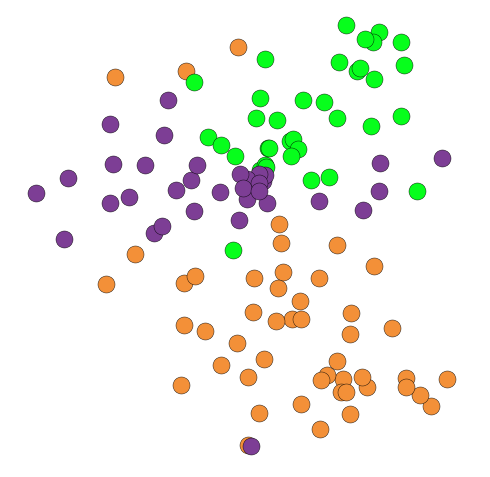
\includegraphics[width=0.23\linewidth , height=0.21\linewidth]{images/tsne_word2vec_raw_cities.png}}
\subcaptionbox{$r$GLV\label{sfig:glove_r_tsne}}{
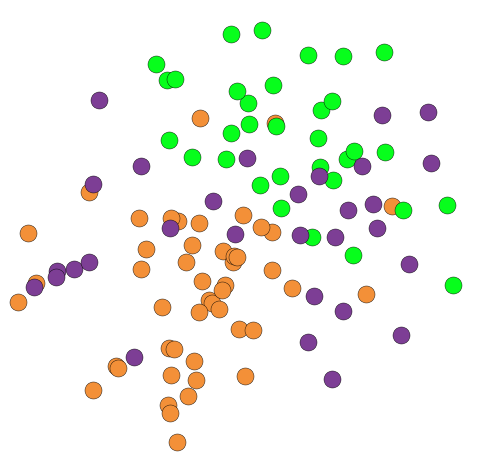
\includegraphics[width=0.23\linewidth , height=0.21\linewidth]{images/tsne_glove_raw_cities.png}}
\subcaptionbox{$a$W2V\label{sfig:word2vec_tsne}}{
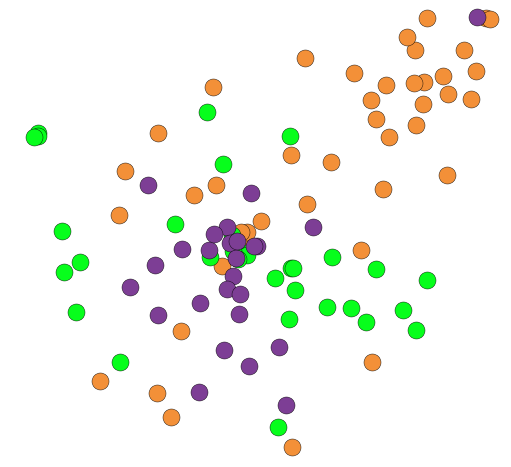
\includegraphics[width=0.23\linewidth , height=0.21\linewidth]{images/tsne_word2vec_cities.png}}
\subcaptionbox{$a$GLV\label{sfig:glove_tsne}}{
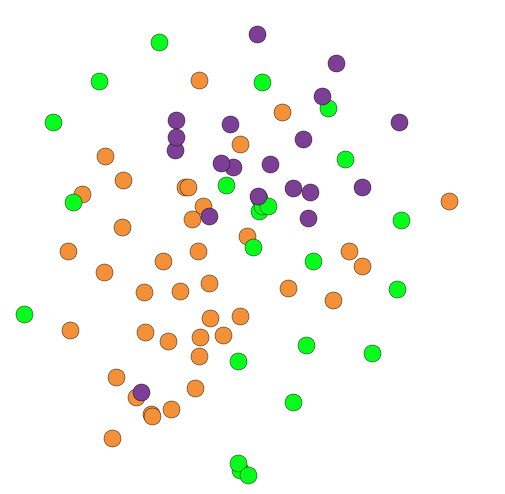
\includegraphics[width=0.23\linewidth , height=0.21\linewidth]{images/tsne_glove_cities.png}}
\subcaptionbox{DW$_{id}$\label{sfig:deepwalk_i_tsne}}{
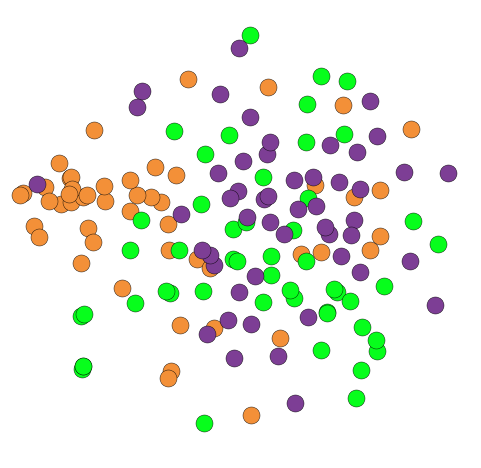
\includegraphics[width=0.23\linewidth , height=0.21\linewidth]{images/tsne_deepwalk_i_cities.png}}
\subcaptionbox{DW$_{log}$\label{sfig:deepwalk_l_tsne}}{
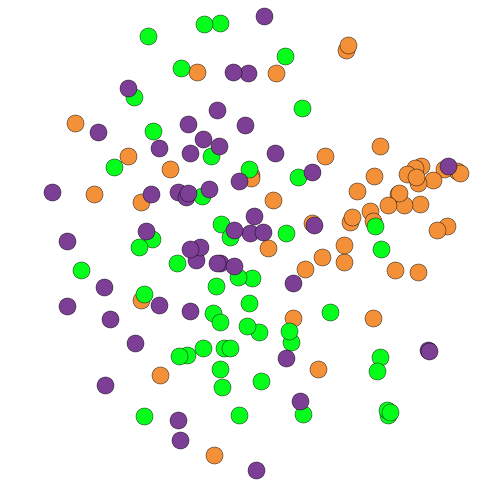
\includegraphics[width=0.23\linewidth , height=0.21\linewidth]{images/tsne_deepwalk_l_cities.png}}
\subcaptionbox{VRS\label{sfig:verse_tsne}}{
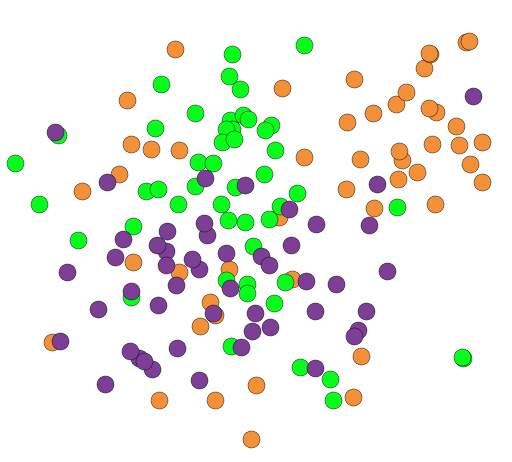
\includegraphics[width=0.23\linewidth , height=0.21\linewidth]{images/tsne_verse_cities.png}}
%\vspace*{-5pt}
\caption{t-SNE projections of the embeddings for U.S.\ (purple), British (orange), and German (green) cities. For the raw text models, multi-word entity names are represented as the mean of word vectors.}
\label{fig:clust}
%\vspace*{-8pt}
\end{figure}

%%%%%%%%%%%%%%%%%%%%%%%%%%%%%%%%%%%%%%%%%%%%%%%%%%%%%%%%%%%%
\subsubsection{Entity neighbourhoods} 
\begin{figure}[t]
\centering
\subcaptionbox{$r$W2V\label{sfig:obama_w2v_r}}{
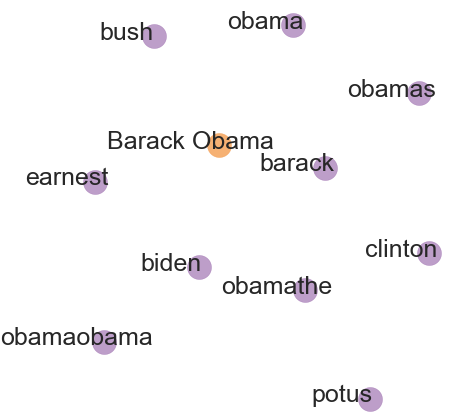
\includegraphics[width=0.30\linewidth , height=0.28\linewidth]{images/obama_w2v_r.png}}\hspace{12pt}%
\subcaptionbox{$a$W2V\label{sfig:obama_w2v}}{
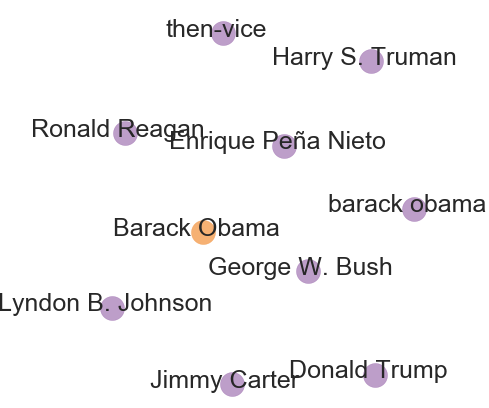
\includegraphics[width=0.30\linewidth , height=0.28\linewidth]{images/obama_w2v.png}}\hspace{12pt}%
\subcaptionbox{VRS\label{sfig:obama_verse}}{
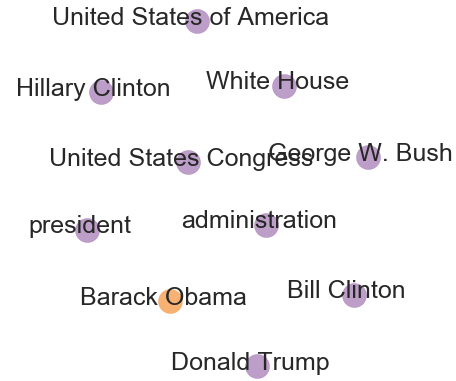
\includegraphics[width=0.30\linewidth , height=0.28\linewidth]{images/obama_verse.png}}
%\vspace*{-5pt}
\caption{t-SNE projections of the nearest neighbours of entity \emph{Barack Obama}.
 % for \emph{w2vec\_r} in  (\subref{sfig:obama_w2v_r}), \emph{w2vec} in  (\subref{sfig:obama_w2v}) and \emph{``Vrs"} in (\subref{sfig:obama_verse}).
}
\label{fig:obama}
%\vspace*{-15pt}
\end{figure}
To understand the neighbourhood relation and proximity of embeddings, we look at most similar words by cosine similarity on the example entity \emph{Barack Obama}. For the raw text models, we average the embeddings of the words \emph{barack} and \emph{obama}. A list of top five words for all models are shown in Table~\ref{tbl:obama}. Entity-based models are more focused on related entities, whereas the the embeddings on raw text tend to focus more on surrounding terms. $r$W2V, in particular, retrieves mostly misspelled versions of the entity name, or separate parts of the name. Since we are using the average of the name parts to represent the entity in vector space, it makes sense that the closest point are the name parts. Top words for the raw model are the most similar words in terms of semantic similarity (mostly synonyms that can be substituted by the entity name in a text), yet, they do not give any further information about possible entity-entity relations. In similar fashion as the relatedness task, we observe that graph-based models on annotated text, VRS in particular, favours relatedness over similarity, as the top retrieved words are the related words that have some association to the entity in question. \\
The Figure~\ref{fig:clust} shows the neighbourhood of top ten closest words to \emph{Barack Obama} for $r$W2V, $a$W2V, and VRS. We observe a similar trend in the 2-dimensional t-SNE projections, where word2vec on raw text tends to primarily identify synonymously used words on the raw corpus (i.e., variations of the entity name) and focuses on similarity. Word2vec on the annotated text, while retrieving more entities also favours similarity, as the nearest neighbours are either other presidents or entities that share similar roles. In contrast, VERSE identifies related entities with different roles, such as administrative locations or the presidential candidates and the president elect in the 2016 U.S.\ election.\\
Overall, for tasks that require word similarity, word embedding methods tend to produce the best result, while the graph-based models have better performance when it comes to identifying relations or associations between entities.
\begin{table}[t]
\caption{Four nearest neighbours of the entity \emph{Barack Obama} with their cosine similarity scores. Entity types include terms T, actors A, and locations L.}
\label{tbl:obama}
\setlength{\tabcolsep}{2pt} % Default value: 6pt
\renewcommand{\arraystretch}{1.0} % Default value: 1
\resizebox{\textwidth}{!}{%
\begin{tabular}{lllllllllllllll}
\toprule
\multicolumn{3}{c}{$r$W2V} & & \multicolumn{3}{c}{$r$GLV} & & \multicolumn{3}{c}{$a$W2V} & & \multicolumn{3}{c}{$a$GLV} \\
\cmidrule(lr){1-3}
\cmidrule(lr){5-7}
\cmidrule(lr){9-11}
\cmidrule(lr){13-15}
T & obama      & 0.90 &&  T & obama          & 0.99 && A & George W. Bush         & 0.76 && T & president      & 0.78 \\
T & barack     & 0.74 &&  T & barack         & 0.98 && A & Jimmy Carter           & 0.73 && T & administration & 0.76 \\
T & obamaobama & 0.68 &&  T & president      & 0.77 && T & barack obama           & 0.73 && A & George W. Bush & 0.72 \\
T & obamathe   & 0.60 &&  T & administration & 0.74 && A & Enrique Pe{\~n}a Nieto & 0.67 && T & mr.            & 0.68 \\
T & bush       & 0.55 &&  T & elect          & 0.66 && T & then-vice              & 0.67 && L & White House    & 0.67 \\
\bottomrule         
\end{tabular}%
}

\hspace*{21pt}
\resizebox{0.87\textwidth}{!}{
\begin{tabular}{lllllllllll}
\toprule
\multicolumn{3}{c}{DW$_{id}$} & & \multicolumn{3}{c}{DW$_{log}$} & & \multicolumn{3}{c}{VRS} \\
\cmidrule(lr){1-3}
\cmidrule(lr){5-7}
\cmidrule(lr){9-11} 
L & White House    & 0.88 && L & White House    & 0.88 && L & White House              & 0.87 \\
T & president      & 0.79 && T & president      & 0.82 && T & president                & 0.79 \\ 
T & presidency     & 0.76 && A & George W. Bush & 0.78 && L & United States of America & 0.76 \\
T & administration & 0.75 && T & administration & 0.78 && A & Donald Trump             & 0.75 \\
A & George W. Bush & 0.74 && T & presidency     & 0.78 && A & Hillary Clinton          & 0.74 \\
\bottomrule
\end{tabular}%
}
\end{table}
\subsection{Analysis of faceted embeddings}\label{subsec:exp_faceted}
To analysis the separate components of faceted embeddings and investigate the semantics behind them, we consider visualizing the clustering task and analysing the neighbourhood for entities. In both cases, we look at the full embeddings with all the components concatenated and also analyse each component separately to understand how the different types of entities surrounding a word can contribute to its semantics and effect its relations to other entities.
%%%%%%%%%%%%%%%%%%%%%%%%%%%%%%%%%%%%%%%%
\subsubsection{Entity clustering} 
One way to understand which component is significant for the representation of entities is to asses which component clusters the similar entities in the embedding. To achieve this, we project the full and partial embeddings of each component for the Cities dataset, which contains location entities, in a 2-dimensional space using t-SNE. The projection for $f$DW$_{log}$ and $f$W2V are shown in Figure~\ref{fig:clust_fword2vec} and Figure~\ref{fig:clust_fdeepwalk}, respectively. The subscript shows the embedding component that is used, e.g., $f$W2V$_{ACT}$ corresponds to faceted word2vec, using only the actor component and $f$W2V indicates the full embedding. Since the performance of $f$DW$_{id}$ and  $f$DW$_{log}$ are similar, we only illustrate the result for $f$DW$_{log}$. For both faceted models, it is not obvious what each component represents. None of the components of $f$DW$_{log}$ form any meaningful cluster, however, the distinction between the three countries is somewhat visible for the location component. The faceted word2vec clearly indicates that dates surrounding a city name are not a good factor for their distinction as all the names are mapped to the same point. Two separate clusters are visible for the location component of $f$W2V, but they are not separated by the county of origin as both clusters are a mixture of all three countries. In general, for the faceted models the visualization of the full embedding is closely related to term component, which is the dominant part in these models.
\begin{figure}[t]
\centering
\subcaptionbox{$f$W2V$_{ACT}$\label{sfig:fword2vec_act_tsne}}{
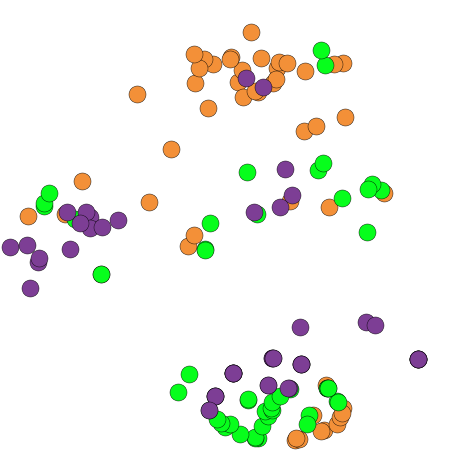
\includegraphics[width=0.23\linewidth , height=0.21\linewidth]{images/fword2vec_act_tsne.png}}
\subcaptionbox{$f$W2V$_{LOC}$\label{fig:fword2vec_loc_tsne}}{
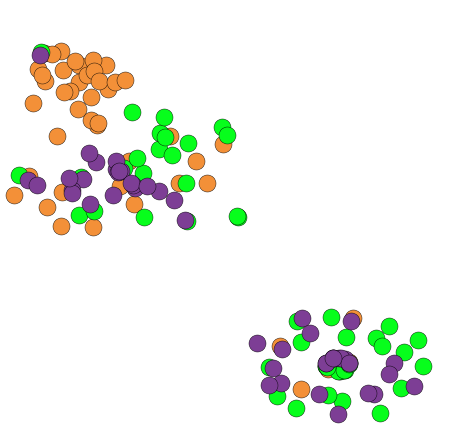
\includegraphics[width=0.23\linewidth , height=0.21\linewidth]{images/fword2vec_loc_tsne.png}}
\subcaptionbox{$f$W2V$_{ORG}$\label{sfig:fword2vec_org_tsne}}{
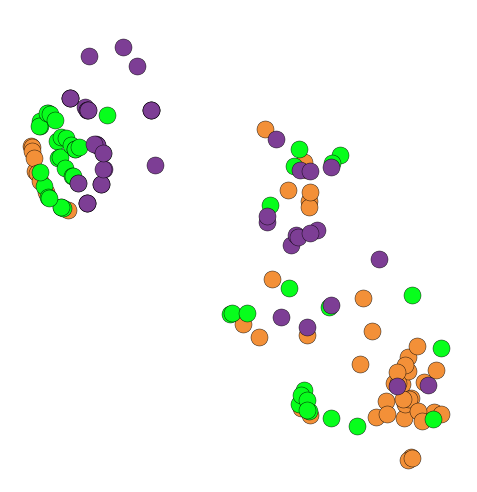
\includegraphics[width=0.23\linewidth , height=0.21\linewidth]{images/fword2vec_org_tsne.png}}
\subcaptionbox{$f$W2V$_{DAT}$\label{sfig:fword2vec_dat_tsne}}{

\includegraphics[width=0.23\linewidth , height=0.21\linewidth]{images/fword2vec_dat_tsne.png}}
\subcaptionbox{$f$W2V$_{TER}$\label{sfig:fword2vec_ter_tsne}}{
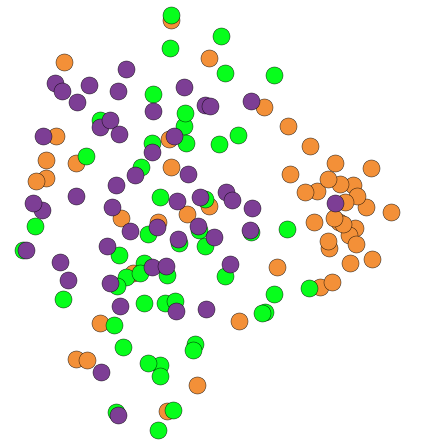
\includegraphics[width=0.23\linewidth , height=0.21\linewidth]{images/fword2vec_ter_tsne.png}}
\subcaptionbox{$f$W2V\label{sfig:fword2vec_tsne}}{
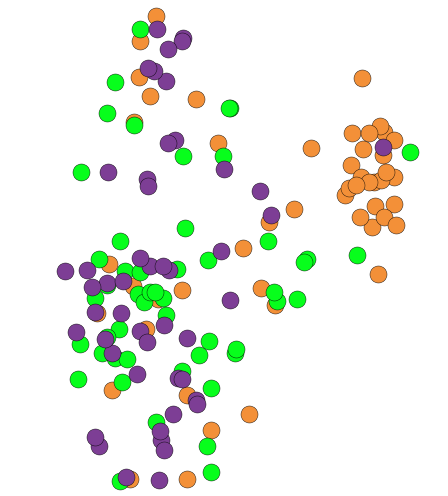
\includegraphics[width=0.23\linewidth , height=0.21\linewidth]{images/fword2vec_tsne.png}}
\caption{t-SNE projections of the embeddings for U.S.\ (purple), British (orange), and German (green) cities, for faceted word2vec using different components.}
\label{fig:clust_fword2vec}
\end{figure}

\begin{figure}[t]
\centering
\subcaptionbox{$f$DW$_{ACT}$\label{sfig:fdeepwalk_act_tsne}}{
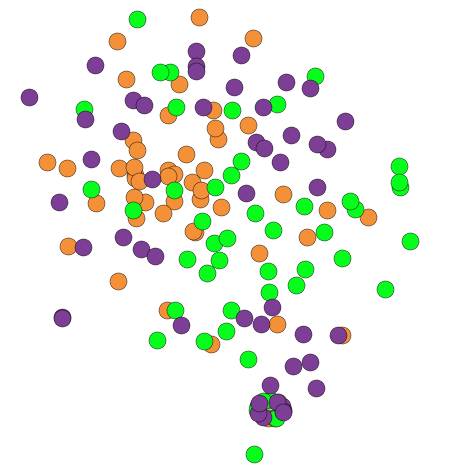
\includegraphics[width=0.23\linewidth , height=0.21\linewidth]{images/fdeepwalk_act_tsne.png}}
\subcaptionbox{$f$DW$_{LOC}$\label{fig:fdeepwalk_loc_tsne}}{
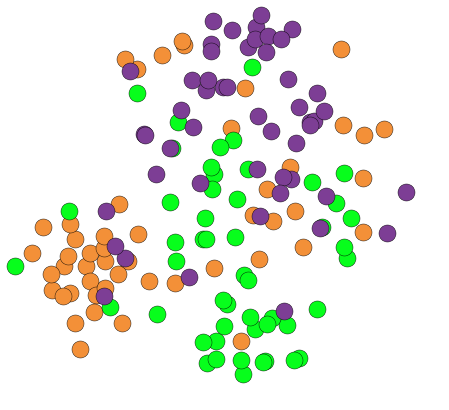
\includegraphics[width=0.23\linewidth , height=0.21\linewidth]{images/fdeepwalk_loc_tsne.png}}
\subcaptionbox{$f$DW$_{ORG}$\label{sfig:fdeepwalk_org_tsne}}{
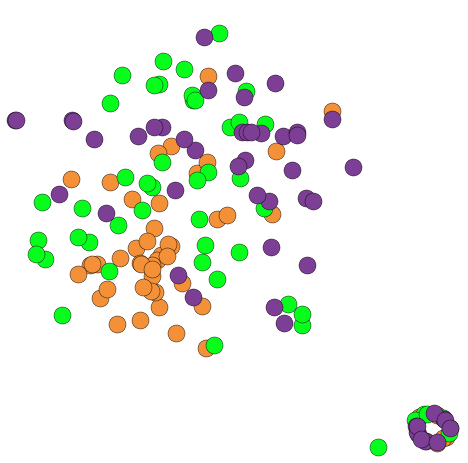
\includegraphics[width=0.23\linewidth , height=0.21\linewidth]{images/fdeepwalk_org_tsne.png}}
\subcaptionbox{$f$DW$_{DAT}$\label{sfig:fdeepwalk_dat_tsne}}{
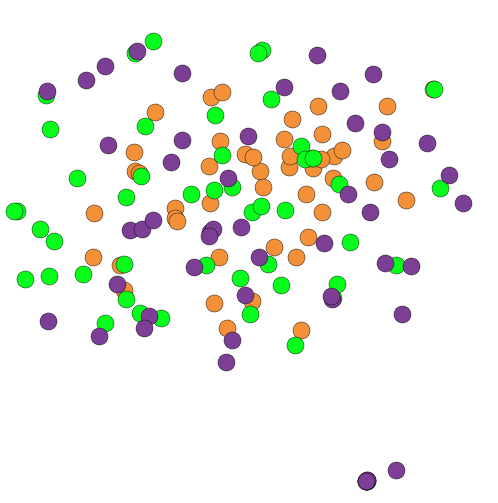
\includegraphics[width=0.23\linewidth , height=0.21\linewidth]{images/fdeepwalk_dat_tsne.png}}
\subcaptionbox{$f$DW$_{TER}$\label{sfig:fdeepwalk_ter_tsne}}{
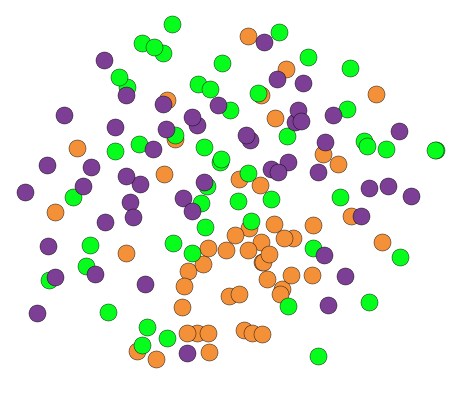
\includegraphics[width=0.23\linewidth , height=0.21\linewidth]{images/fdeepwalk_ter_tsne.png}}
\subcaptionbox{$f$DW\label{sfig:fdeepwalk_tsne}}{
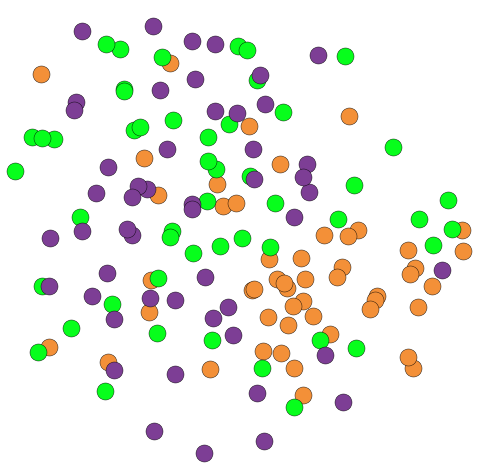
\includegraphics[width=0.23\linewidth , height=0.21\linewidth]{images/fdeepwalk_tsne.png}}
\caption{t-SNE projections of the embeddings for U.S.\ (purple), British (orange), and German (green) cities, for faceted deepwalk with logarithmic normalization using different components.}
\label{fig:clust_fdeepwalk}
\end{figure}

%%%%%%%%%%%%%%%%%%%%%%%%%%%%%%%%%%%%%%%%%%%%%%%%%%%%%%%%%%%%
\subsubsection{Entity neighbourhoods} 
\begin{figure}[t]
\centering
\subcaptionbox{$r$W2V\label{sfig:obama_w2v_r}}{
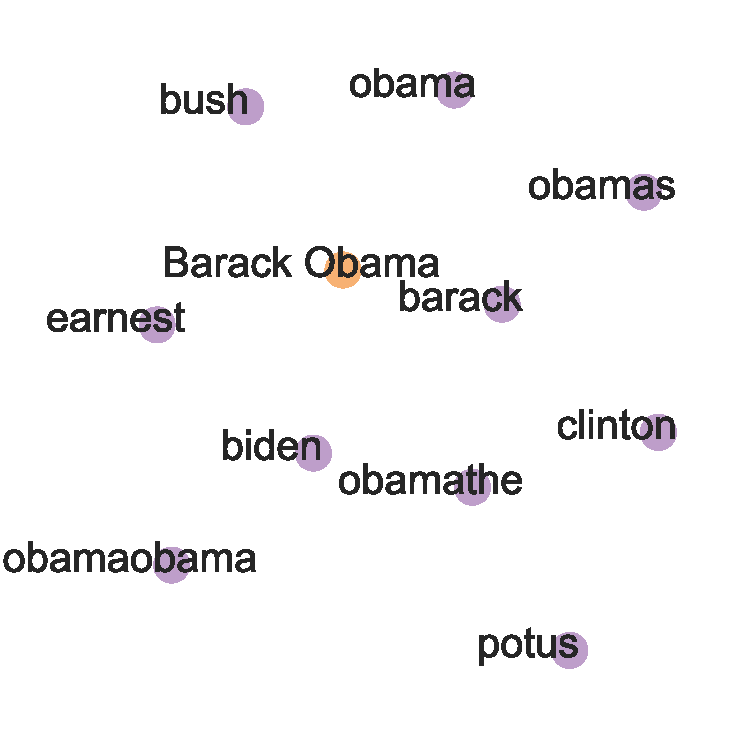
\includegraphics[width=0.30\linewidth , height=0.28\linewidth]{images/obama_w2v_r.pdf}}\hspace{12pt}%
\subcaptionbox{$f$W2V\label{sfig:obama_fw2v}}{
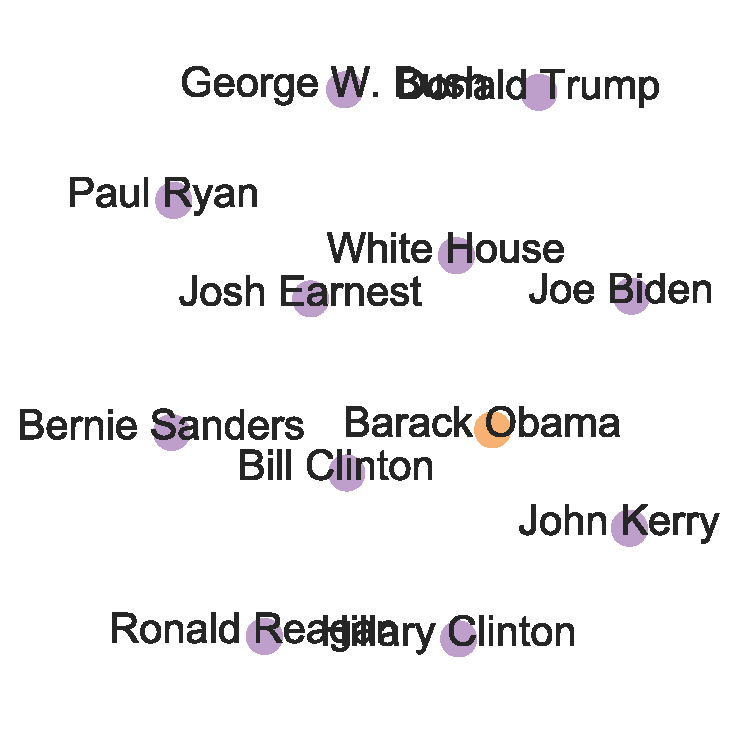
\includegraphics[width=0.30\linewidth , height=0.28\linewidth]{images/obama_fw2v.pdf}}\hspace{12pt}%
\subcaptionbox{$f$DW$_{log}$\label{sfig:obama_fdw}}{
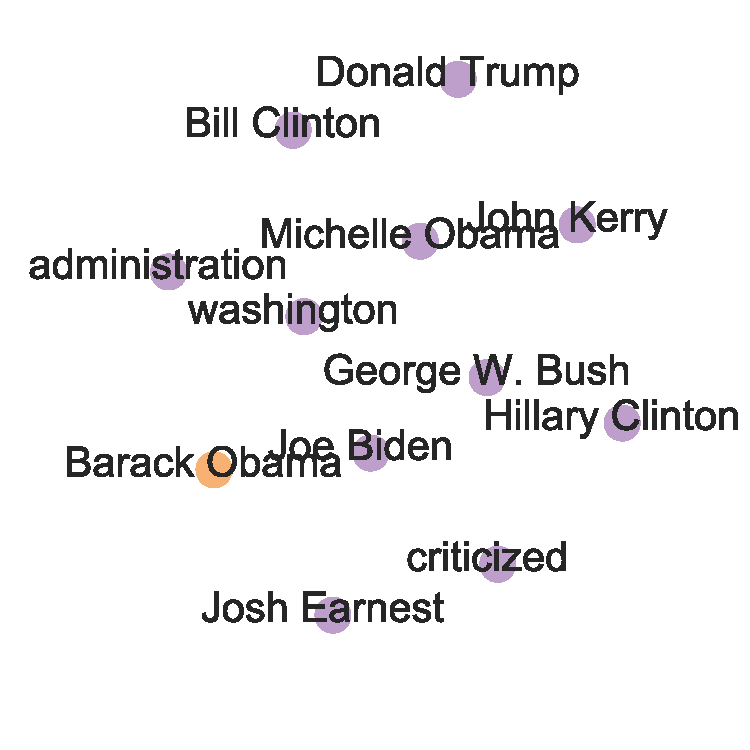
\includegraphics[width=0.30\linewidth , height=0.28\linewidth]{images/obama_fdw.pdf}}
\caption{t-SNE projections of the nearest neighbours of entity \emph{Barack Obama} for faceted embeddings.}
\end{figure}
\label{fig:obama_faceted}
%\vspace*{-15pt}
To analyse the proximity of embeddings based on different components, we investigate the most similar words by cosine similarity to the example actor entity \emph{Barach Obama}. A list of top five words for the faceted models with full embeddings and $r$W2V and $r$GLV is shown in Table~\ref{tbl:obama_faceted}. Same as the entity embeddings, the faceted models are more focused on entity relations, whereas the word embeddings on raw text retrieve synonymous terms. Although the $f$DW$_{id}$ tends to contain some terms in the top result, with the log normalization the result become close to $f$W2V, which mostly contains former presidents, the presidential candidate for the 2016 election and other democrat politicians. The projection of the neighbourhood for $r$W2V, $f$DW$_{log}$, and $f$W2V is shown in Figure~\ref{fig:obama_faceted}. While the faceted models tend to focus on entity-entity relations, $r$W2V retrieves the miss-spelled versions of the name and last names of former presidents. Without the knowledge of the query word it is not obvious if the word \emph{bush} refers to the entity \emph{George W.Bush} or the whole \emph{Bush} family or even the plant. On the other hand, faceted models, despite a few terms like \emph{administration}, contain mostly associated politicians.\\
In Table~\ref{tbl:obama_faceted_p} we look at the top five results based on separate components for $f$W2V and $f$DW$_{log}$, where the subscript indicates the component that is used to find the nearest neighbours. $f$DW$_{id}$ produces similar results and, thus, is not demonstrated. We observe an interesting trend in $f$W2V, where the type of the most similar entity to a word is dependent on the component type. Most similar entities to \emph{Barack Obama} in the date components are dates themselves, including $2005$ when his career in the United States Senate began. The same applies for locations, organisations and actors, where the majority of retrieved entities share the type of the component. For example, locations such as South Sudan in the location component or \emph{United States Congress} for the organisation. It appears that the topic of the attack on the embassy in \emph{Benghazi} is dominant in the data as the raid happened on the date $2011-07-09$. Important political actors related to this event were former National Security Advisor \emph{Ben Rhodes} and the former State Secretary \emph{Hillary Clinton}, which were all in the administration of \emph{Barack Obama}. In case of $f$DW$_{log}$, the effect of component type is less visible, with only the actor component containing only actors as its top five. These actors have no obvious connection to \emph{Barack Obama}, except \emph{Glenn Hutchins}, who was an advisor to \emph{Bill Clinton} and probably for that reason shows up in the result. The unrelated results of DeepWalk based models may lie in the structure of the co-occurrence graph and the type-restricted random walk, which was introduced to limit the context. Since we restricted the random walk to only edges that have a specific entity type as the end node for each component we focus on very limited information. For example, to perform a type restricted random walk for actors from the start node of \emph{Barack Obama}, we retrieve actors that are connected through other actors, which is not necessary helpful. Therefore, results, such as \emph{Glenn Hutchins} that are not a result of direct connection show up in the result.
\begin{table}[t]
\caption{Four nearest neighbours of the entity \emph{Barack Obama} with cosine similarity scores for faceted models and embeddings on raw text. Entity types include terms T and actors A.}
\label{tbl:obama_faceted}
\setlength{\tabcolsep}{1.5pt} % Default value: 6pt
\renewcommand{\arraystretch}{1.0} % Default value: 1
\resizebox{\textwidth}{!}{%
\begin{tabular}{lllllllllllllllllll}
\toprule
\multicolumn{3}{c}{$r$W2V} & & \multicolumn{3}{c}{$r$GLV} & & \multicolumn{3}{c}{$f$W2V} & & \multicolumn{3}{c}{$f$DW$_{id}$} & & \multicolumn{3}{c}{$f$DW$_{log}$}\\
\cmidrule(lr){1-3}
\cmidrule(lr){5-7}
\cmidrule(lr){9-11}
\cmidrule(lr){13-15}
\cmidrule(lr){17-19}
T & obama      & 0.90 &&  T & obama     & 0.99 && A & Donald Trump & 0.92    && A & Donald Trump & 0.84&& A& Hillary Clinton & 0.85 \\
T & barack     & 0.74 &&  T & barack         & 0.98 && A & Hillary Clinton & 0.91 && A & Hillary Clinton & 0.84 && A & Donald Trump & 0.85\\
T & obamaobama & 0.68 &&  T & president      & 0.77 && A & Bill Clinton & 0.89 && T & nation & 0.83 && A & Bill Clinton & 0.83\\
T & obamathe   & 0.60 &&  T & administration & 0.74 && A & Bernie Sanders & 0.87 && T & force & 0.83 && A & Josh Earnest & 0.82 \\
T & bush       & 0.55 &&  T & elect          & 0.66 && A & George W. Bush & 0.87 && T & freedom & 0.82 && T & administration & 0.82\\
\bottomrule         
\end{tabular}%
}
\end{table}



\begin{table}[t]
\caption{Four nearest neighbours of entity \emph{Barack Obama} with cosine similarity scores. For separate components of $f$W2V and $f$DW$_{log}$. Entity types include terms T, actors A , and locations L, organisations O, dates D.}
\label{tbl:obama_faceted_p}
\setlength{\tabcolsep}{1.5pt} % Default value: 6pt
\renewcommand{\arraystretch}{1.0} % Default value: 1
\resizebox{\textwidth}{!}{%
\begin{tabular}{lllllllllllllllllll}
\toprule
\multicolumn{3}{c}{$f$W2V$_{TER}$} & & \multicolumn{3}{c}{$f$W2V$_{ACT}$} & & \multicolumn{3}{c}{$f$W2V$_{LOC}$} & & \multicolumn{3}{c}{$f$W2V$_{ORG}$} & & \multicolumn{3}{c}{$f$W2V$_{DAT}$}\\
\cmidrule(lr){1-3}
\cmidrule(lr){5-7}
\cmidrule(lr){9-11}
\cmidrule(lr){13-15}
\cmidrule(lr){17-19}
L &White House & 0.97&& L & White House & 0.98 && T & 0324 & 0.77  && A & White House & 0.97&& D & 2016-01-26 & 0.64 \\
T & democratic & 0.96&&  A & Donald Trump & 0.92&& L & St. John's Episcopal Church & 0.76 && A & Donald Trump & 0.93 && D & 2008-06-08 & 0.57\\
T & presidential & 0.95 &&  L & Washington, D.C. & 0.92&& D & 2011-07-09 & 0.73 && O & U.S.\ House of Representatives & 0.93 && D & 2005 & 0.56\\
A & George W. Bush & 0.94 && A & Ben Rhodes & 0.91&& L & South Sudan & 0.72 && O & U.S.\ Congress & 0.93 && D & 1865-05 & 0.56 \\
T & republican & 0.94&&  A & Hillary Clinton & 0.91 && L & Palazzo Grassi & 0.71&& A & Hillary Clinton & 0.93&& D & 1970 & 0.55\\
\bottomrule         
\end{tabular}%
}

\resizebox{\textwidth}{!}{
\begin{tabular}{lllllllllllllllllll}
\toprule
\multicolumn{3}{c}{$f$DW$_{TER}$} & & \multicolumn{3}{c}{$f$DW$_{ACT}$} & & \multicolumn{3}{c}{$f$DW$_{LOC}$} & & \multicolumn{3}{c}{$f$DW$_{ORG}$} & & \multicolumn{3}{c}{$f$DW$_{DAT}$}\\
\cmidrule(lr){1-3}
\cmidrule(lr){5-7}
\cmidrule(lr){9-11}
\cmidrule(lr){13-15}
\cmidrule(lr){17-19}
L &Philadelphia & 0.94&& A & Daniel M. Ashe & 0.92 && T & decades & 0.97  && A & Bill Clinton & 0.97&& T & not & 0.99 \\
L & Pennsylvania & 0.94&&  A & Hefty Stuart & 0.90&& T & reported & 0.97 && L & New York City & 0.96 && L & Alabama & 0.99\\
D & 2016-07 & 0.92 &&  A & Elena Bromund & 0.90&& T & statement & 0.96 && T & according & 0.95 && T & party & 0.99\\
L & New York City & 0.92 && A & Brendan O'Connor & 0.90&& T & rally & 0.96 && A & Donald Trump & 0.95 && T & timeline & 0.98 \\
O & United States Congress & 0.92 &&  A & Glenn Hutchins & 0.90 && T & according & 0.96&& L & Benghazi & 0.95&& T & kept & 0.98\\
\bottomrule         
\end{tabular}%
}
\end{table}
\section{Summary}\label{sec:eval_summary}
In this chapter, we reported the results of intrinsic evaluation on entity embeddings and faceted embeddings, we compare them against the state-of-the-art word embedding methods on popular term-based intrinsic tasks. In addition, we investigated the characteristics of each method through exploratory analysis and visualization.\\
In general, while the word embedding on raw text captures the similarity among words well, they tend to map the synonymous words closer in the embedding space, while models on the annotated corpus (faceted and entity embeddings) focus on association among entities. Models that use the co-occurrence graphs from annotated text as input, in particular, focus on relatedness and are more entity oriented, and tend to produce better results on entity-centric analogy task. In addition, they are able retrieve associated entities with a neighbourhood search. \\
Faceted models share many similarity with the entity embedding, in terms of capturing relatedness and good performance on entity-centric analogy task. However, overall they perform poorly on most word similarity and categorization tasks. These models retrieve related entities with a neighbourhood search and have the extra advantage of separable components. Through studying the component separately, we show that for the most term-based intrinsic task the most important entity type is term. Although components other than term are not significant for the term-based evaluations, they can be used to search the neighbourhood of a word based on entity types. $f$W2V is notably good at retrieving entities of a particular type with nearest neighbour search in the relevant subspace.
%-----removed parts 
%
%\begin{figure}
%\centering
%\subcaptionbox{\label{sfig:full_wordsim}}{
%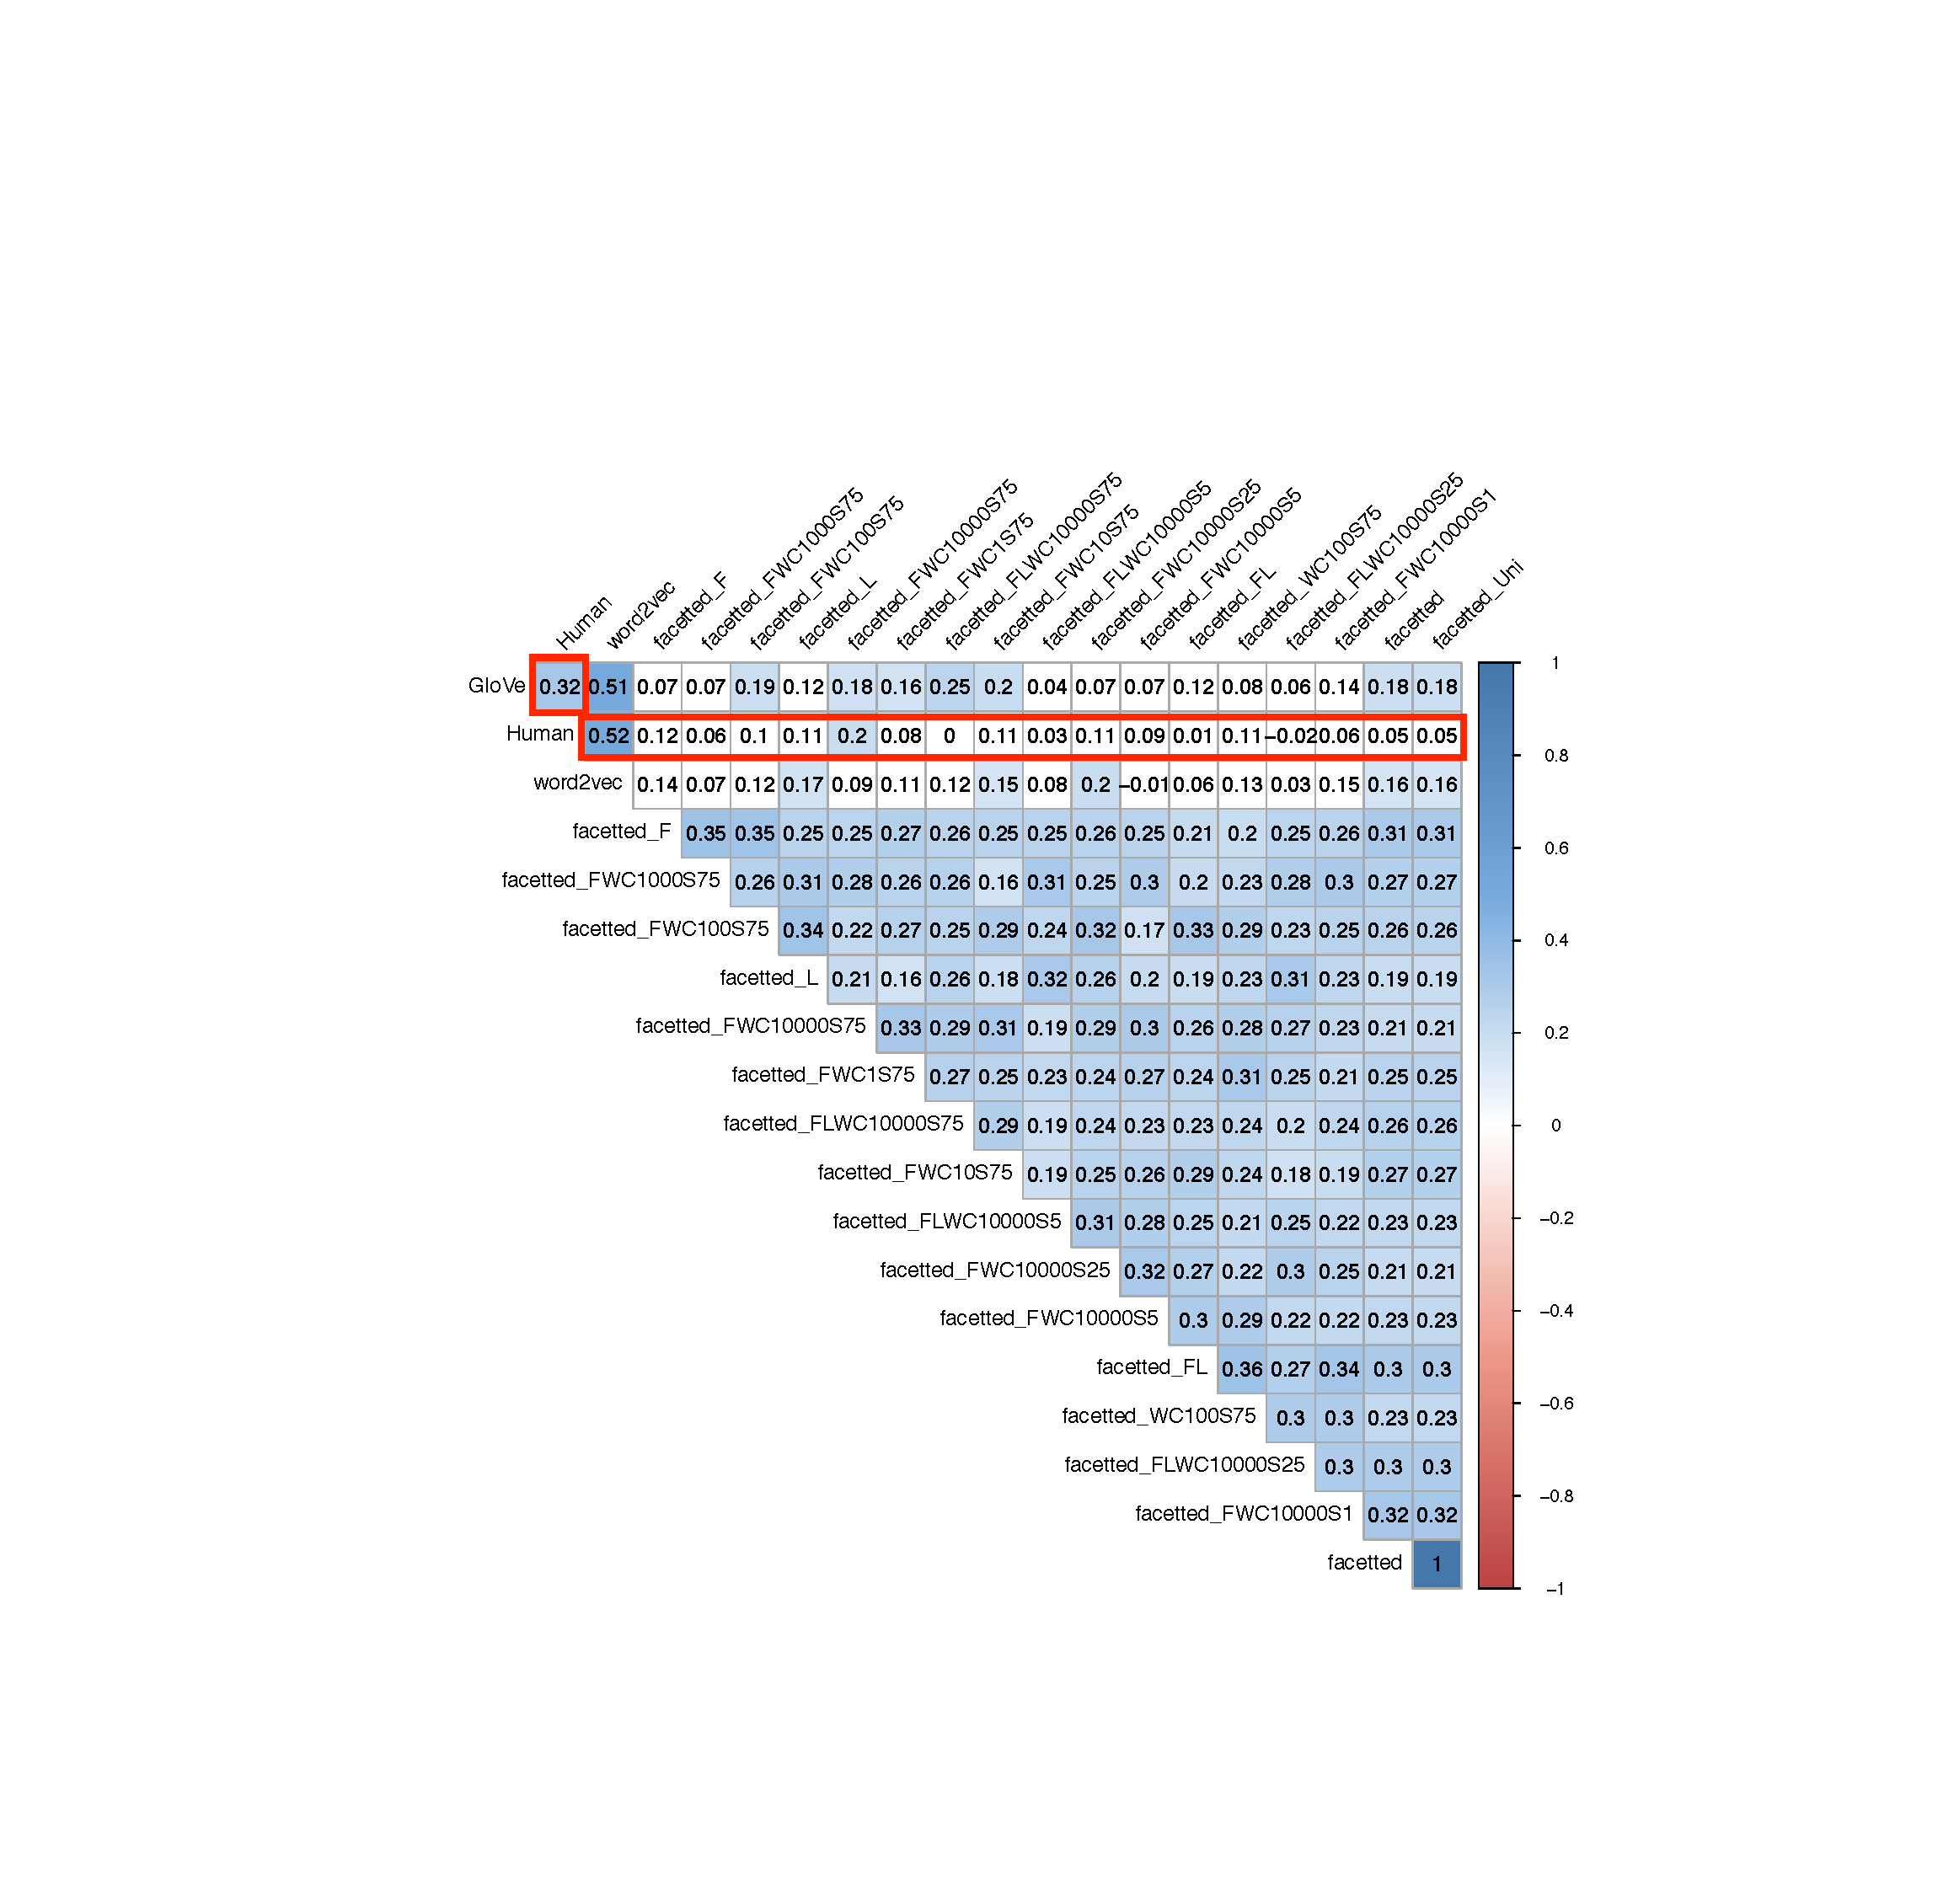
\includegraphics[width=0.75\linewidth , height=0.65\linewidth]{images/Corr_plot_full_sim.pdf}}
%\subcaptionbox{\label{sfig:part_wordsim}}{
%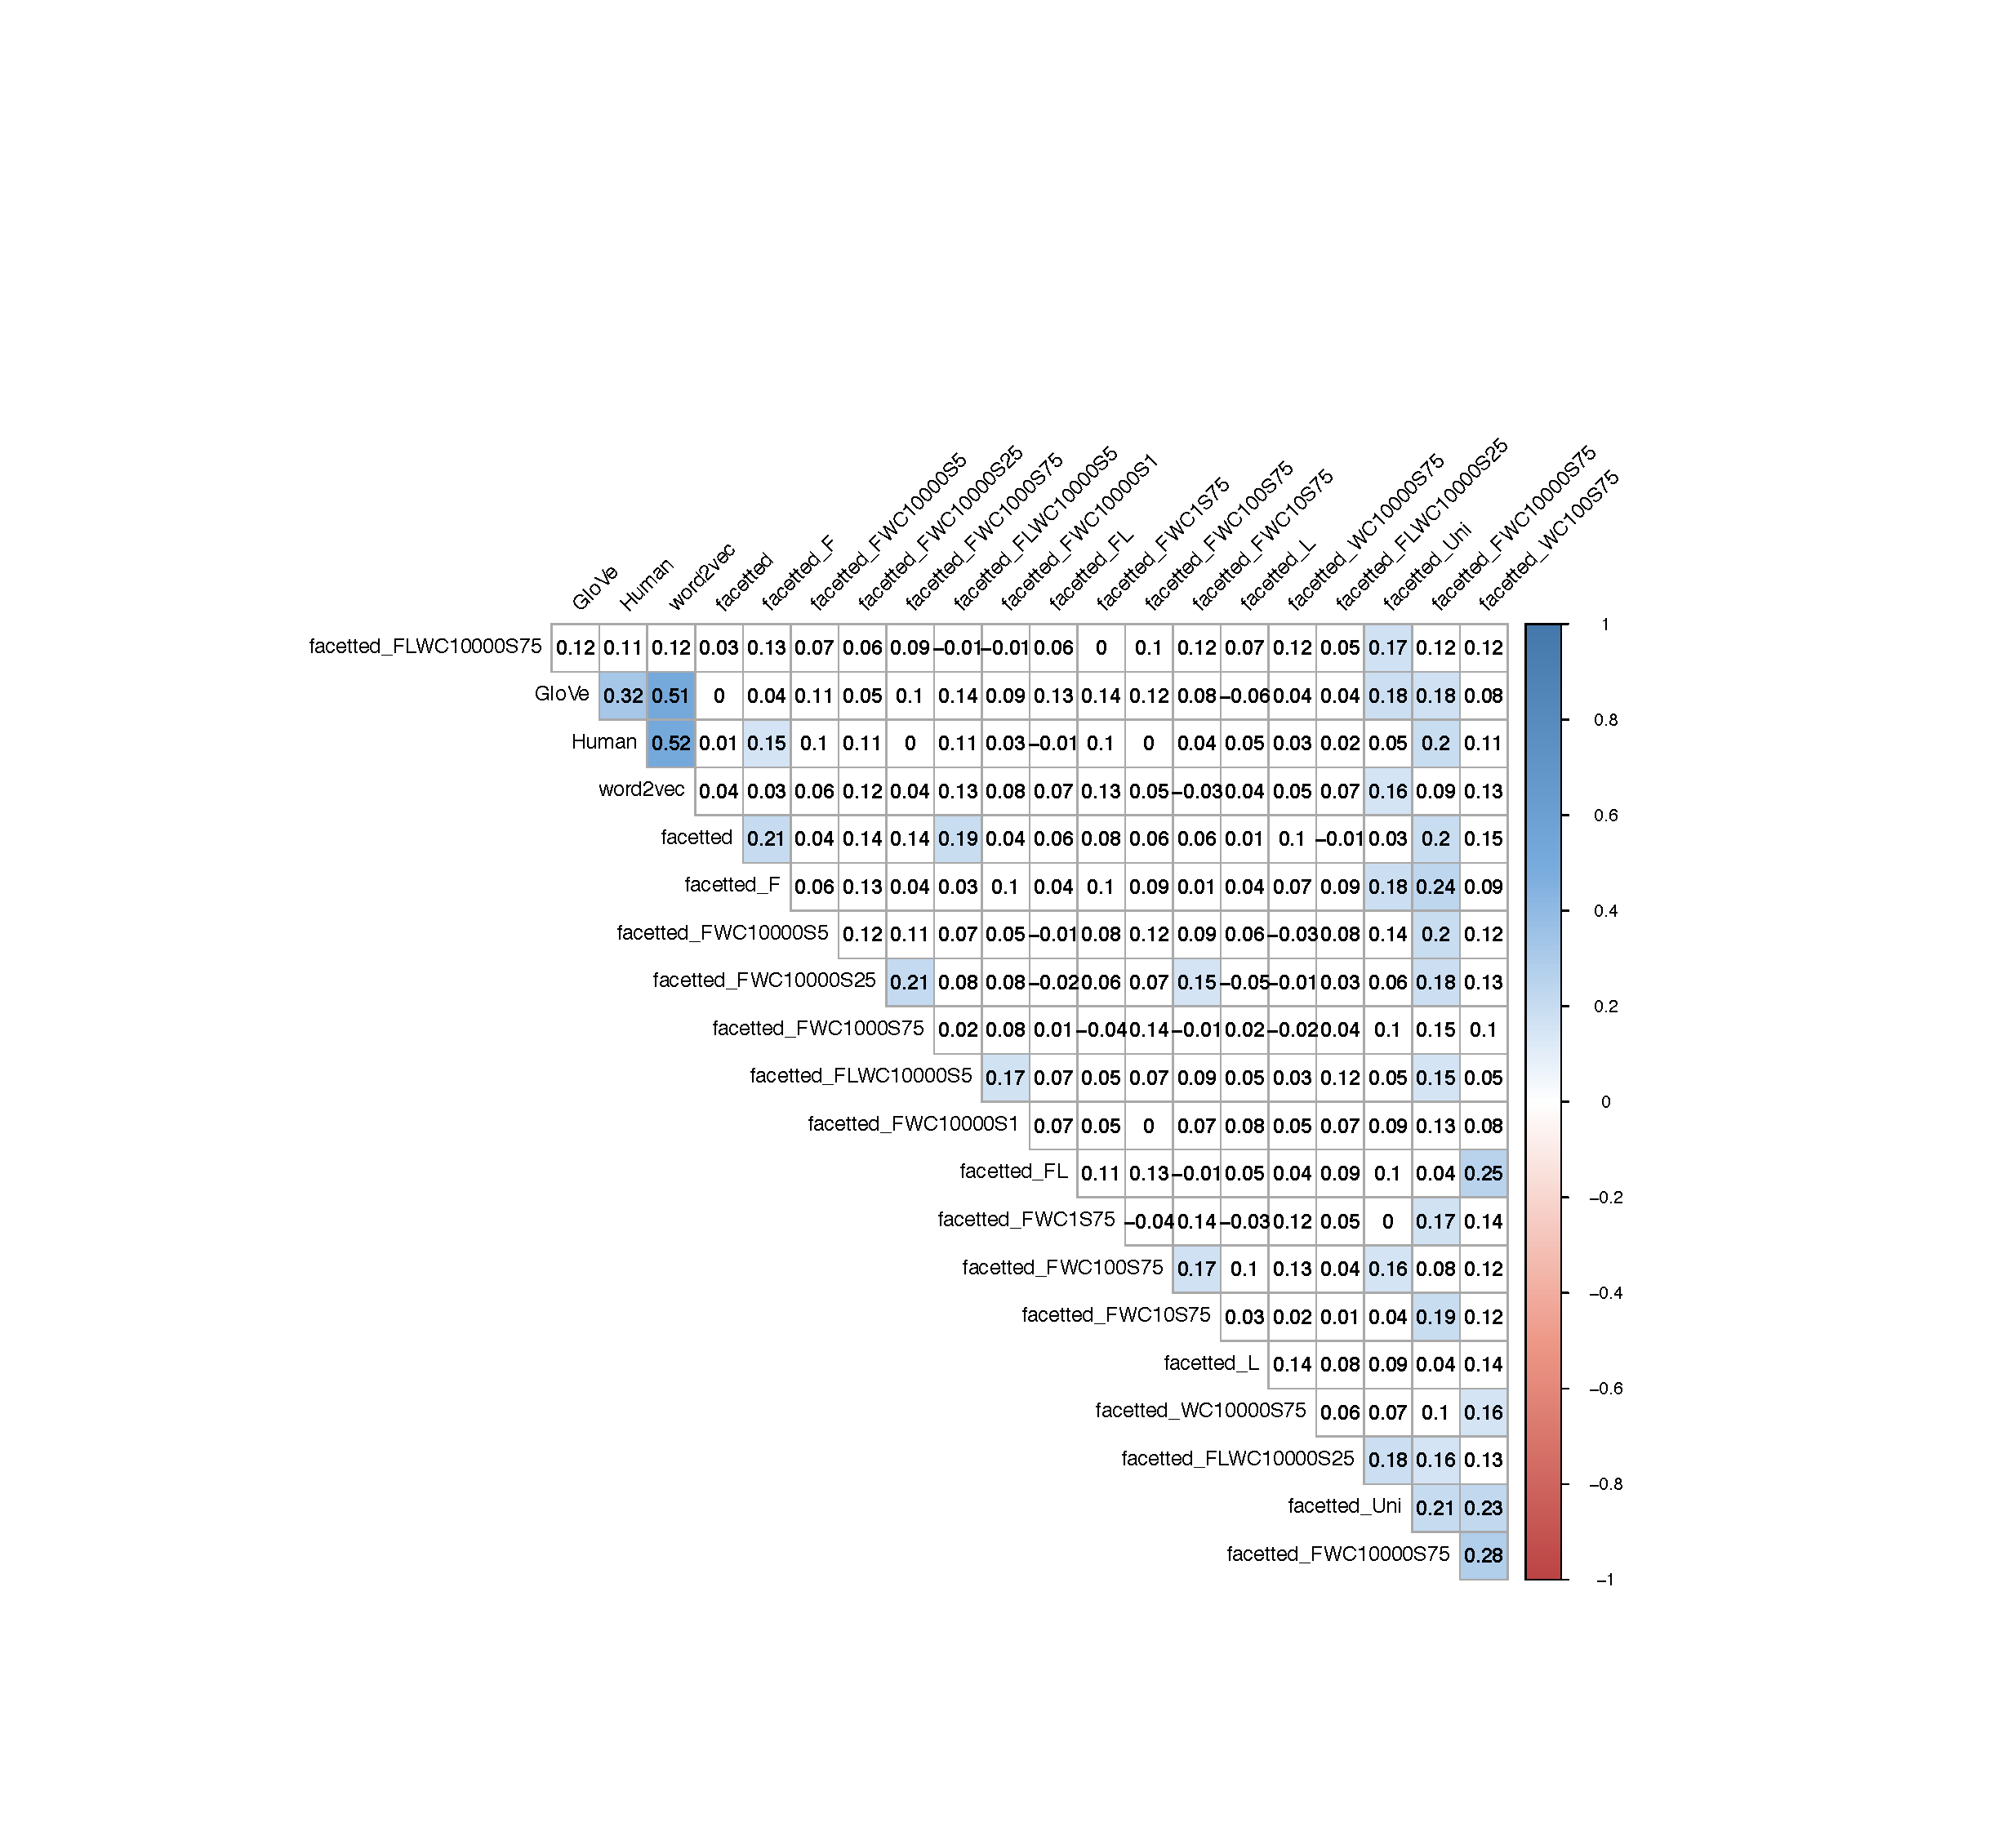
\includegraphics[width=0.80\linewidth , height=0.65\linewidth]{images/wordsim_partial.pdf}}
%
%\caption{Correlation plot of the relatedness scores on wordsim353 using the~\subref{sfig:full_wordsim} full vectors and ~\subref{sfig:part_wordsim} using type-specific vectors. Red highlights show the correlation with the human annotations.}
%\label{fig:wordsim_cor}
%\end{figure}
%
%
%%\begin{figure}
%\centering
%\subcaptionbox{\label{sfig:word2vec_tsne}}{
%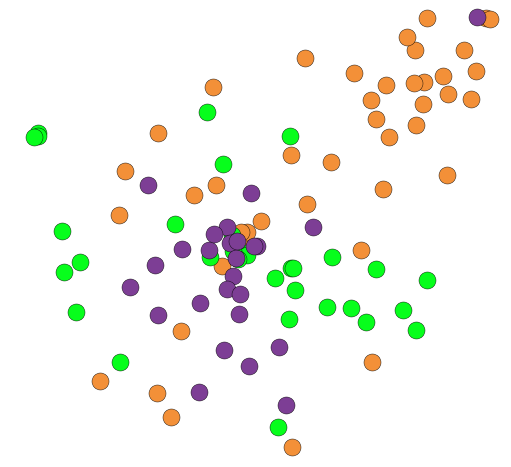
\includegraphics[width=0.48\linewidth , height=0.5\linewidth]{images/tsne_word2vec_cities.png}}
%\subcaptionbox{\label{sfig:glove_tsne}}{
%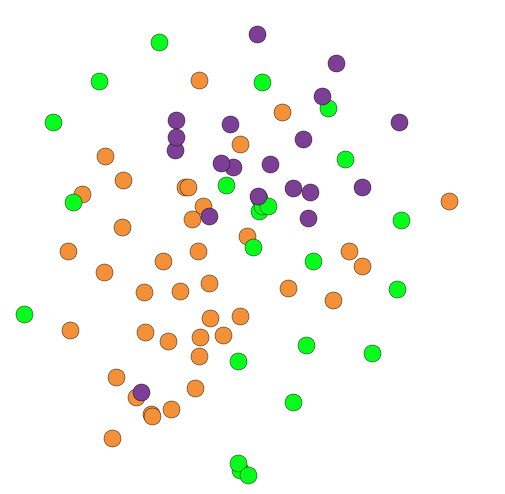
\includegraphics[width=0.48\linewidth , height=0.5\linewidth]{images/tsne_glove_cities.png}}
%\subcaptionbox{\label{sfig:complex_tsne}}{
%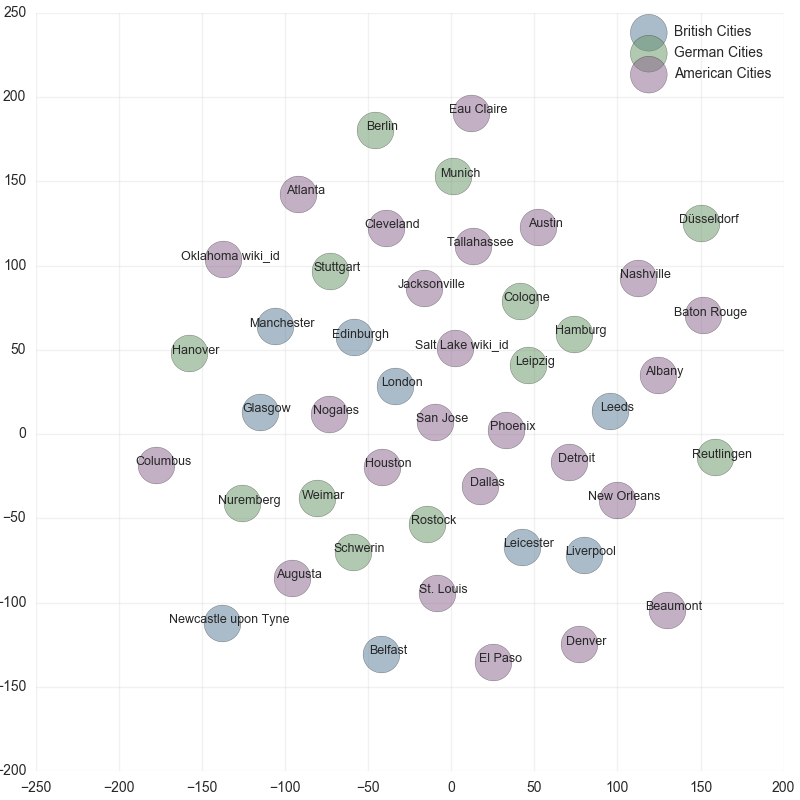
\includegraphics[width=0.5\linewidth , height=0.5\linewidth]{images/tsne_complex_cities.png}}
%
%\caption{t-SNE projections of the embeddings:\subref{sfig:word2vec_tsne} German, British and American cities using Word2Vec \subref{sfig:glove_tsne} GloVe and \subref{sfig:complex_tsne} facetted\_FWC10000S75.}
%\label{fig:clust}
%\end{figure}
%
%
%\begin{table}[h]
%  \centering
%  {%
%    \raisebox{1.5cm}{%
%      \begin{tabular}{lSS}
%        \toprule
%        {Algorithm }                     & {Accuracy}   \\
%        \midrule
%        Facetted\_FWC10000S75   &0        \\
%        GloVe    & 0.008     \\
%        word2vec   & 0.015       \\
%        \bottomrule
%      \end{tabular}
%    }
%  }
%  \caption{The accuracy results on Mikolove's test set with $9,968$ word pairs.}
%  \label{table:analogy}
%\end{table}
%
%
%\begin{figure}[hb]
%\centering
%\subcaptionbox{\label{sfig:scaling_f}}{
%\resizebox{0.45\textwidth}{0.30\textwidth}{      
%
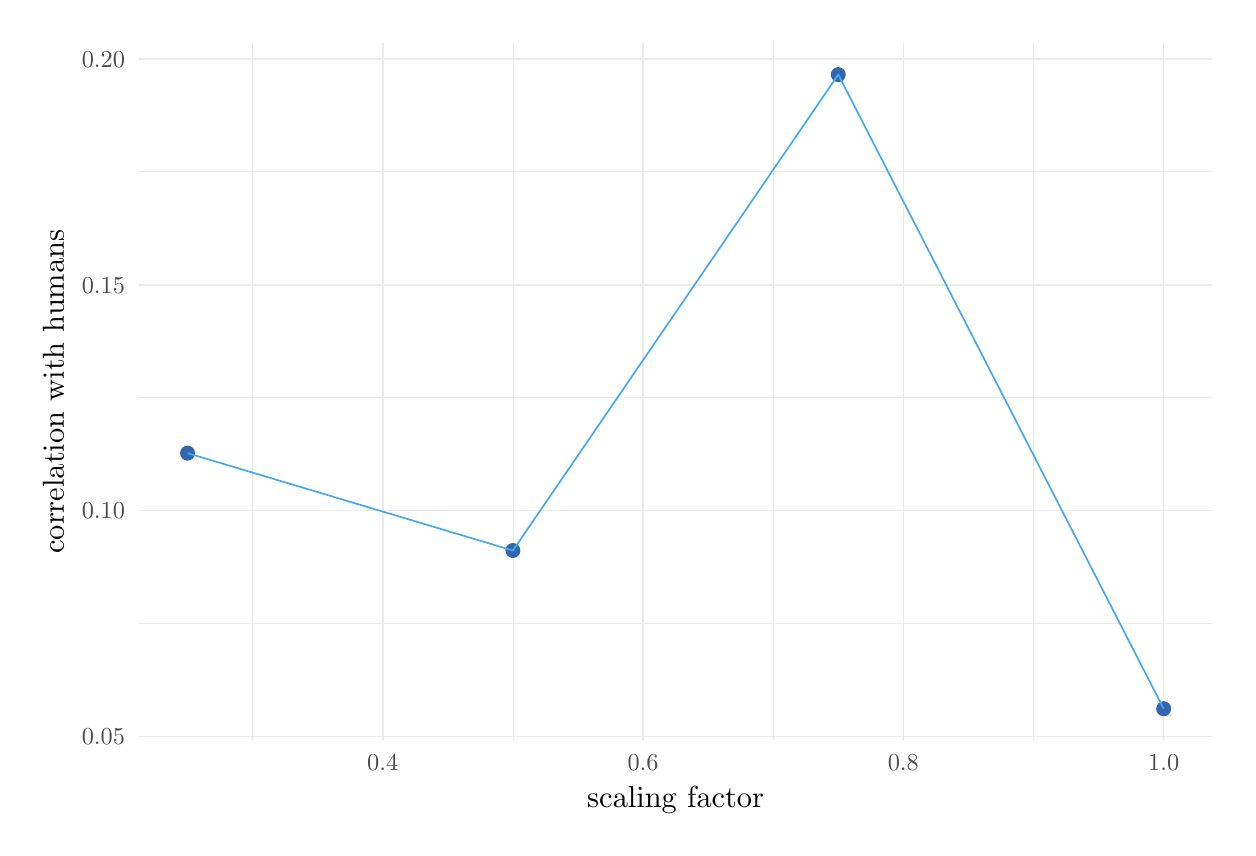
\begin{tikzpicture}[x=1pt,y=1pt]
\definecolor{fillColor}{RGB}{255,255,255}
\path[use as bounding box,fill=fillColor,fill opacity=0.00] (0,0) rectangle (433.62,289.08);
\begin{scope}
\path[clip] ( 40.14, 31.53) rectangle (428.12,283.58);
\definecolor{drawColor}{gray}{0.92}

\path[draw=drawColor,line width= 0.3pt,line join=round] ( 40.14, 73.78) --
	(428.12, 73.78);

\path[draw=drawColor,line width= 0.3pt,line join=round] ( 40.14,155.37) --
	(428.12,155.37);

\path[draw=drawColor,line width= 0.3pt,line join=round] ( 40.14,236.97) --
	(428.12,236.97);

\path[draw=drawColor,line width= 0.3pt,line join=round] ( 81.29, 31.53) --
	( 81.29,283.58);

\path[draw=drawColor,line width= 0.3pt,line join=round] (175.34, 31.53) --
	(175.34,283.58);

\path[draw=drawColor,line width= 0.3pt,line join=round] (269.40, 31.53) --
	(269.40,283.58);

\path[draw=drawColor,line width= 0.3pt,line join=round] (363.46, 31.53) --
	(363.46,283.58);

\path[draw=drawColor,line width= 0.6pt,line join=round] ( 40.14, 32.98) --
	(428.12, 32.98);

\path[draw=drawColor,line width= 0.6pt,line join=round] ( 40.14,114.58) --
	(428.12,114.58);

\path[draw=drawColor,line width= 0.6pt,line join=round] ( 40.14,196.17) --
	(428.12,196.17);

\path[draw=drawColor,line width= 0.6pt,line join=round] ( 40.14,277.76) --
	(428.12,277.76);

\path[draw=drawColor,line width= 0.6pt,line join=round] (128.32, 31.53) --
	(128.32,283.58);

\path[draw=drawColor,line width= 0.6pt,line join=round] (222.37, 31.53) --
	(222.37,283.58);

\path[draw=drawColor,line width= 0.6pt,line join=round] (316.43, 31.53) --
	(316.43,283.58);

\path[draw=drawColor,line width= 0.6pt,line join=round] (410.48, 31.53) --
	(410.48,283.58);
\definecolor{drawColor}{RGB}{50,103,173}
\definecolor{fillColor}{RGB}{50,103,173}

\path[draw=drawColor,line width= 0.4pt,line join=round,line cap=round,fill=fillColor] ( 57.77,135.33) circle (  2.50);

\path[draw=drawColor,line width= 0.4pt,line join=round,line cap=round,fill=fillColor] (175.34,100.15) circle (  2.50);

\path[draw=drawColor,line width= 0.4pt,line join=round,line cap=round,fill=fillColor] (292.91,272.12) circle (  2.50);

\path[draw=drawColor,line width= 0.4pt,line join=round,line cap=round,fill=fillColor] (410.48, 42.99) circle (  2.50);
\definecolor{drawColor}{RGB}{66,167,244}

\path[draw=drawColor,line width= 0.6pt,line join=round] ( 57.77,135.33) --
	(175.34,100.15) --
	(292.91,272.12) --
	(410.48, 42.99);
\end{scope}
\begin{scope}
\path[clip] (  0.00,  0.00) rectangle (433.62,289.08);
\definecolor{drawColor}{gray}{0.30}

\node[text=drawColor,anchor=base east,inner sep=0pt, outer sep=0pt, scale=  0.88] at ( 35.19, 29.95) {0.05};

\node[text=drawColor,anchor=base east,inner sep=0pt, outer sep=0pt, scale=  0.88] at ( 35.19,111.55) {0.10};

\node[text=drawColor,anchor=base east,inner sep=0pt, outer sep=0pt, scale=  0.88] at ( 35.19,193.14) {0.15};

\node[text=drawColor,anchor=base east,inner sep=0pt, outer sep=0pt, scale=  0.88] at ( 35.19,274.73) {0.20};
\end{scope}
\begin{scope}
\path[clip] (  0.00,  0.00) rectangle (433.62,289.08);
\definecolor{drawColor}{gray}{0.30}

\node[text=drawColor,anchor=base,inner sep=0pt, outer sep=0pt, scale=  0.88] at (128.32, 20.52) {0.4};

\node[text=drawColor,anchor=base,inner sep=0pt, outer sep=0pt, scale=  0.88] at (222.37, 20.52) {0.6};

\node[text=drawColor,anchor=base,inner sep=0pt, outer sep=0pt, scale=  0.88] at (316.43, 20.52) {0.8};

\node[text=drawColor,anchor=base,inner sep=0pt, outer sep=0pt, scale=  0.88] at (410.48, 20.52) {1.0};
\end{scope}
\begin{scope}
\path[clip] (  0.00,  0.00) rectangle (433.62,289.08);
\definecolor{drawColor}{RGB}{0,0,0}

\node[text=drawColor,anchor=base,inner sep=0pt, outer sep=0pt, scale=  1.10] at (234.13,  7.44) {scaling factor};
\end{scope}
\begin{scope}
\path[clip] (  0.00,  0.00) rectangle (433.62,289.08);
\definecolor{drawColor}{RGB}{0,0,0}

\node[text=drawColor,rotate= 90.00,anchor=base,inner sep=0pt, outer sep=0pt, scale=  1.10] at ( 13.08,157.56) {correlation with humans};
\end{scope}
\end{tikzpicture}


%}}
%\subcaptionbox{\label{sfig:weight_cap}}{\resizebox{0.45\textwidth}{0.30\textwidth}{      
%
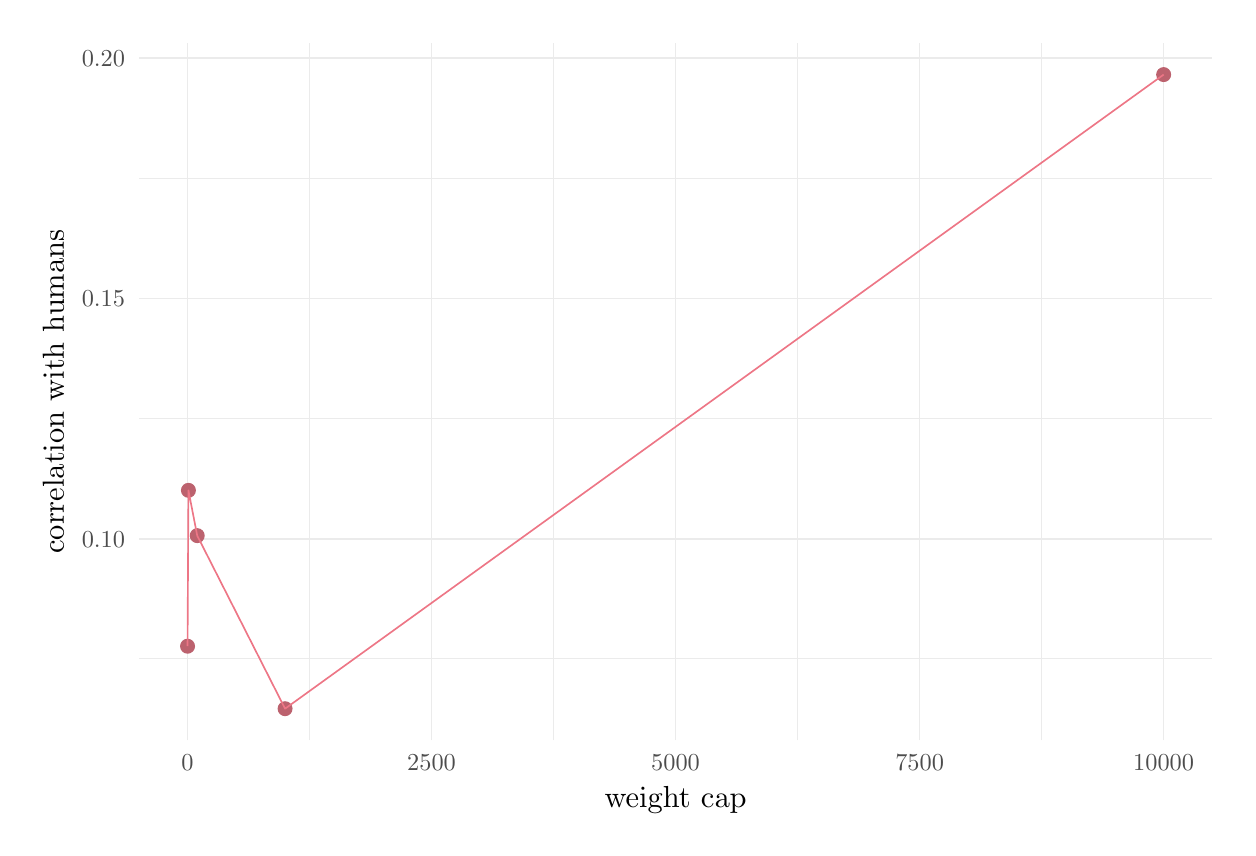
\begin{tikzpicture}[x=1pt,y=1pt]
\definecolor{fillColor}{RGB}{255,255,255}
\path[use as bounding box,fill=fillColor,fill opacity=0.00] (0,0) rectangle (433.62,289.08);
\begin{scope}
\path[clip] ( 40.14, 31.53) rectangle (428.12,283.58);
\definecolor{drawColor}{gray}{0.92}

\path[draw=drawColor,line width= 0.3pt,line join=round] ( 40.14, 60.99) --
	(428.12, 60.99);

\path[draw=drawColor,line width= 0.3pt,line join=round] ( 40.14,147.85) --
	(428.12,147.85);

\path[draw=drawColor,line width= 0.3pt,line join=round] ( 40.14,234.70) --
	(428.12,234.70);

\path[draw=drawColor,line width= 0.3pt,line join=round] (101.83, 31.53) --
	(101.83,283.58);

\path[draw=drawColor,line width= 0.3pt,line join=round] (190.02, 31.53) --
	(190.02,283.58);

\path[draw=drawColor,line width= 0.3pt,line join=round] (278.20, 31.53) --
	(278.20,283.58);

\path[draw=drawColor,line width= 0.3pt,line join=round] (366.39, 31.53) --
	(366.39,283.58);

\path[draw=drawColor,line width= 0.6pt,line join=round] ( 40.14,104.42) --
	(428.12,104.42);

\path[draw=drawColor,line width= 0.6pt,line join=round] ( 40.14,191.27) --
	(428.12,191.27);

\path[draw=drawColor,line width= 0.6pt,line join=round] ( 40.14,278.13) --
	(428.12,278.13);

\path[draw=drawColor,line width= 0.6pt,line join=round] ( 57.74, 31.53) --
	( 57.74,283.58);

\path[draw=drawColor,line width= 0.6pt,line join=round] (145.93, 31.53) --
	(145.93,283.58);

\path[draw=drawColor,line width= 0.6pt,line join=round] (234.11, 31.53) --
	(234.11,283.58);

\path[draw=drawColor,line width= 0.6pt,line join=round] (322.30, 31.53) --
	(322.30,283.58);

\path[draw=drawColor,line width= 0.6pt,line join=round] (410.48, 31.53) --
	(410.48,283.58);
\definecolor{drawColor}{RGB}{188,98,110}
\definecolor{fillColor}{RGB}{188,98,110}

\path[draw=drawColor,line width= 0.4pt,line join=round,line cap=round,fill=fillColor] ( 57.77, 65.57) circle (  2.50);

\path[draw=drawColor,line width= 0.4pt,line join=round,line cap=round,fill=fillColor] ( 58.09,121.89) circle (  2.50);

\path[draw=drawColor,line width= 0.4pt,line join=round,line cap=round,fill=fillColor] ( 61.27,105.52) circle (  2.50);

\path[draw=drawColor,line width= 0.4pt,line join=round,line cap=round,fill=fillColor] ( 93.01, 42.99) circle (  2.50);

\path[draw=drawColor,line width= 0.4pt,line join=round,line cap=round,fill=fillColor] (410.48,272.12) circle (  2.50);
\definecolor{drawColor}{RGB}{237,118,134}

\path[draw=drawColor,line width= 0.6pt,line join=round] ( 57.77, 65.57) --
	( 58.09,121.89) --
	( 61.27,105.52) --
	( 93.01, 42.99) --
	(410.48,272.12);
\end{scope}
\begin{scope}
\path[clip] (  0.00,  0.00) rectangle (433.62,289.08);
\definecolor{drawColor}{gray}{0.30}

\node[text=drawColor,anchor=base east,inner sep=0pt, outer sep=0pt, scale=  0.88] at ( 35.19,101.39) {0.10};

\node[text=drawColor,anchor=base east,inner sep=0pt, outer sep=0pt, scale=  0.88] at ( 35.19,188.24) {0.15};

\node[text=drawColor,anchor=base east,inner sep=0pt, outer sep=0pt, scale=  0.88] at ( 35.19,275.10) {0.20};
\end{scope}
\begin{scope}
\path[clip] (  0.00,  0.00) rectangle (433.62,289.08);
\definecolor{drawColor}{gray}{0.30}

\node[text=drawColor,anchor=base,inner sep=0pt, outer sep=0pt, scale=  0.88] at ( 57.74, 20.52) {0};

\node[text=drawColor,anchor=base,inner sep=0pt, outer sep=0pt, scale=  0.88] at (145.93, 20.52) {2500};

\node[text=drawColor,anchor=base,inner sep=0pt, outer sep=0pt, scale=  0.88] at (234.11, 20.52) {5000};

\node[text=drawColor,anchor=base,inner sep=0pt, outer sep=0pt, scale=  0.88] at (322.30, 20.52) {7500};

\node[text=drawColor,anchor=base,inner sep=0pt, outer sep=0pt, scale=  0.88] at (410.48, 20.52) {10000};
\end{scope}
\begin{scope}
\path[clip] (  0.00,  0.00) rectangle (433.62,289.08);
\definecolor{drawColor}{RGB}{0,0,0}

\node[text=drawColor,anchor=base,inner sep=0pt, outer sep=0pt, scale=  1.10] at (234.13,  7.44) {weight cap};
\end{scope}
\begin{scope}
\path[clip] (  0.00,  0.00) rectangle (433.62,289.08);
\definecolor{drawColor}{RGB}{0,0,0}

\node[text=drawColor,rotate= 90.00,anchor=base,inner sep=0pt, outer sep=0pt, scale=  1.10] at ( 13.08,157.56) {correlation with humans};
\end{scope}
\end{tikzpicture}


%}}
%
%\caption{\subref{sfig:scaling_f} Effect of scaling factor for facetted embeddings on the correlation on wordsim353. \subref{sfig:weight_cap} Effect of weight cap for facetted embeddings on the correlation on wordsim353.}
%\label{fig:correlation_change}
%\end{figure}
%
%
%\begin{figure}
%\centering
%\subcaptionbox{\label{sfig:full_men}}{
%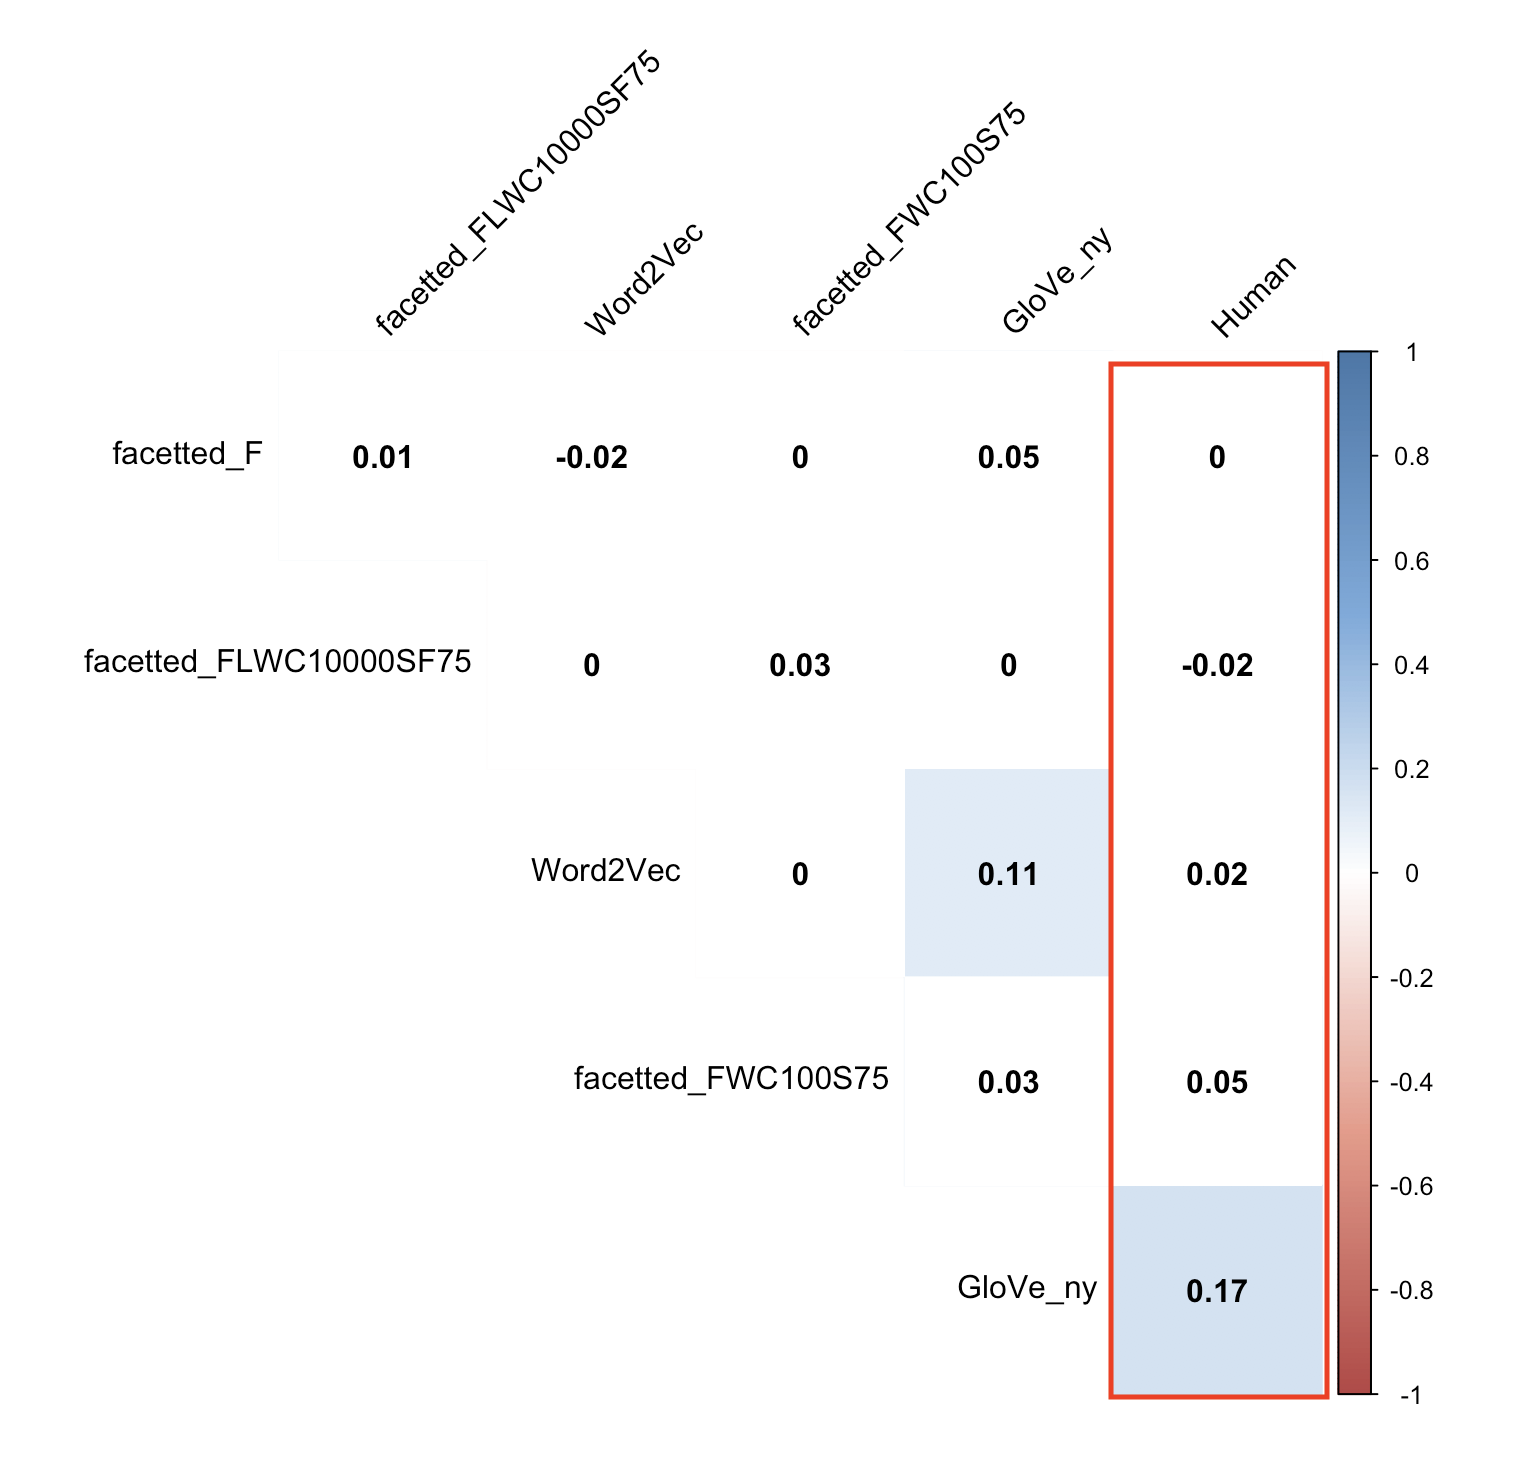
\includegraphics[width=0.7\linewidth , height=0.6\linewidth]{images/men_full.pdf}}
%\subcaptionbox{\label{sfig:part_men}}{
%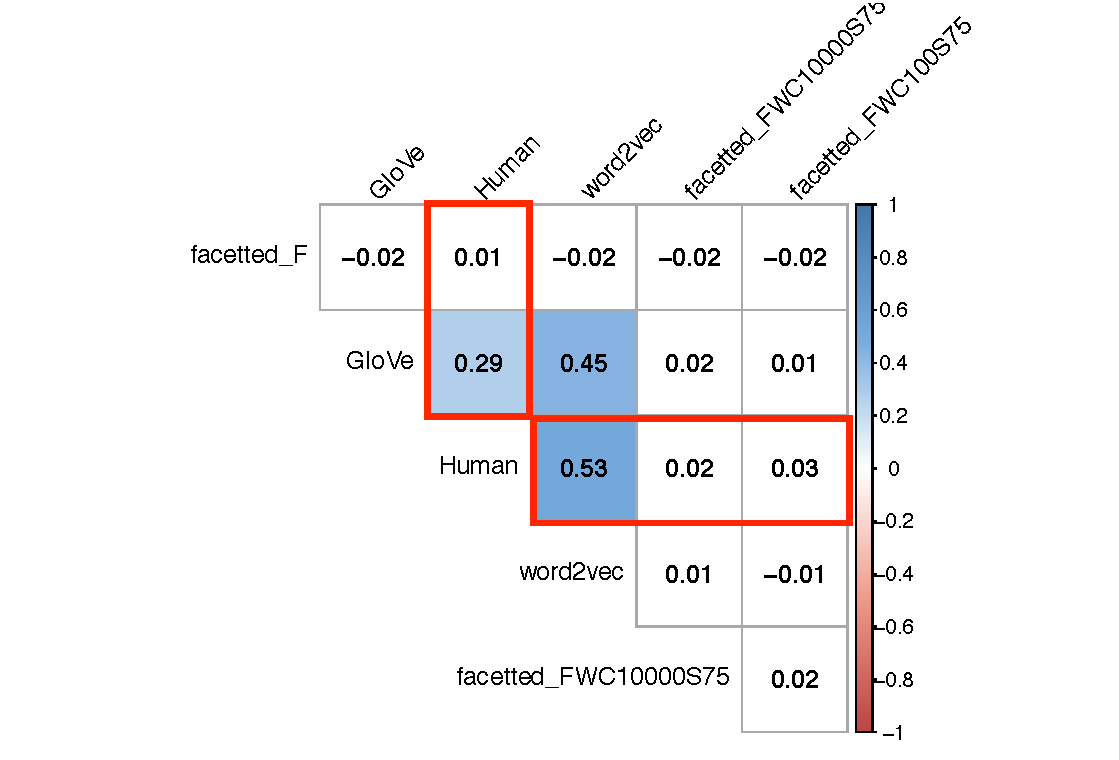
\includegraphics[width=0.7\linewidth , height=0.6\linewidth]{images/men_part.pdf}}
%
%\caption{Correlation plot of the relatedness scores on MEN using the~\subref{sfig:full_men} full vectors and ~\subref{sfig:part_men} using type-specific vectors. Red highlights show the correlation with the human annotations.}
%\label{fig:men_cor}
%\end{figure}

  %%%%%%%%%%%%%%%%%%%%%%%%%%%%%%%%%%%%%%%%%%%%%%%%%%%%%%%%%%%%
\chapter{Conclusions}\label{chap:concl}
The weights of LOAD, similar to co-occurrence matrices, contain information about the statistics of the corpus and meaningful components can be extracted from them. In spite of this similarity using the weighted adjacency matrix for separate types of entities and then combining the results is unable to beat the state of the art models on common embedding tasks. The true potential of these embeddings might be visible in using them in a specific downstream task. As to what the dimensions really capture in these embeddings, not a meaningful explanation could be found in the visualizations. \\
One possible explanation for the relatively poor performance of the facetted model can be simply lack of information to learn from. For each type, the vocabulary is limited to a certain type and thus removing other surrounding words and limiting the context. \\



% This ensures that the subsequent sections are being included as root
% items in the bookmark structure of your PDF reader.
\bookmarksetup{startatroot}
\backmatter

  \begingroup
    \let\clearpage\relax
    \glsaddall
    \printglossary[type=\acronymtype]
    \newpage
    \printglossary
  \endgroup

  \printindex

  \printbibliography

\end{document}
